% ******************************************************** %
% DOCUMENT INFORMATION                                     %
% ******************************************************** %
%                                                          %
%                                                          %
% Purpose of Document                                      %
% -------------------                                      %
% Technical Report                                         %
%                                                          %
% Institution                                              %
% -----------                                              %
% University of Applied Sciences and Arts Northwestern     %
% Switzerland, School of Engineering                       %
%                                                          %
% Degree Program                                           %
% --------------                                           %
% Electrical Engineering and Information Technology, BSc.  %
%                                                          %
% Course                                                   %
% ------                                                   %
% Project 4, Spring Semester 2016                          %
%                                                          %
% Authors                                                  %
% -------                                                  %
% Marcel Heymann     (Firmware)                            %
% Noah Hüsser        (Hardware, Firmware)                  %
% Raphael Frey       (Simulations, Reporting)              %
% Dominik Keller     (Hardware, Firmware)                  %
% Marco Koch         (Deputy Team Leader, Simulations)     %
% Reto Nussbaumer    (Team Leader)                         %
% Francesco Rovelli  (Hardware, Firmware)                  %
%                                                          %
% Document Design and Maintenance                          %
% -------------------------------                          %
% Raphael Frey                                             %
% Based on my own work. The  template on which this report %
% was based is available at:                               %
% https://github.com/alpenwasser/longtex                   %
% -------------------------------------------------------- %

\documentclass[11pt, a4paper, oneside]{memoir}

% -------------------------------------------------------- %
% Different font and pages  sizes, layouts. Not a complete %
% list, just what I've used on occasion.                   %
% -------------------------------------------------------- %
%\documentclass[9pt,b5paper]{memoir}
%\documentclass[twocolumn,9pt,a4paper]{memoir}
%\documentclass[10pt,a5paper]{memoir} % ~60 chars per line
%\documentclass[12pt,a4paper]{memoir} % ~60 to 70 chars per line


% -------------------------------------------------------- %
% Preamble  stuff  is  kept in  the  preamble/  directory, %
% separated  out into  different files  as needed  to keep %
% things modular.                                          %
% -------------------------------------------------------- %
% -------------------------------------------------------- %
% NOTE: There   are  two   kinds  of   packages  in   this %
% document. On ond hand, there  are those which are needed %
% for this  template to function at  as intended. It might %
% still  compile without  them,  but it  will probably  no %
% longer look as it should.                                %
%                                                          %
% On the other hand, there are those which I have found to %
% be useful over the years  and tend to commonly use.  You %
% may or may  not need those.  Feel free  to disable those %
% you do not need.                                         %
%                                                          %
% By default,  I recommend leaving the  following packages %
% enabled:                                                 %
% - fontenc: for output font encoding                      %
% - inputenc: for using  non-standard characters in input, %
%   such as Umlauts or other accented characters           %
% - graphicx:  needed for  the  chapter  style (based  on  %
%   veelo)                                                 %
%                                                          %
% Feel free to  disable and enable the  rest as needed. If %
% the document no longer compiles or breaks aesthetically, %
% you will notice soon enough...                           %
% -------------------------------------------------------- %


% -------------------------------------------------------- %
% General Packages                                         %
% -------------------------------------------------------- %
\usepackage[T1]{fontenc}     % output encoding
\usepackage[utf8]{inputenc}  % input encoding
\usepackage[ngerman]{babel}
\usepackage{lipsum}          % filler text
\usepackage{graphicx}
\usepackage{amsmath}         % for reasonable math typesetting
\usepackage{pdfpages}        % include pdf documents
%\usepackage{amsfonts}        % not sure yet if we need this
\usepackage{adjustbox}       % helps w/ minipage alignmant
\usepackage[textsize=footnotesize, textwidth = 37mm, german, colorinlistoftodos]{todonotes}
\usepackage{calc}            % used for calculating margins and widths for A3 pages
%\usepackage{caption}         % captions outside float environments, overrides memoir's caption facilities
\usepackage[separate-uncertainty=true]{siunitx}
\usepackage[light]{kpfonts}
\usepackage{counttexruns}
\usepackage[european,siunitx,cuteinductors]{circuitikz}


% -------------------------------------------------------- %
% Draft Watermark                                          %
%                                                          %
% Prints  a watermark  across the  page, marking  it as  a %
% draft.                                                   %
% -------------------------------------------------------- %
\usepackage{draftwatermark}
\SetWatermarkText{Entwurf, \today}
\SetWatermarkScale{0.5}
%\usepackage[final]{draftwatermark} % removes watermark



% -------------------------------------------------------- %
% TIKZ and PGF                                             %
%                                                          %
% TODO: See if this  should be put in a  separate file, or %
% if  having  it  here makes  sense. Alternatively,  these %
% documents might not need to be set globally at all.      %
% -------------------------------------------------------- %
\usepackage{tikz}
\usetikzlibrary{arrows}
\usetikzlibrary{decorations.pathmorphing}
\usepackage{pgfplots}
\pgfplotsset{compat=newest}
\pgfplotsset{max space between ticks=80pt}
\pgfplotsset{max space between ticks=80pt}
\pgfplotsset{try min ticks=5}
\pgfplotsset{
    tick label style={font=\small},
    label style={font=\small},
    legend style={font=\footnotesize}
}


% -------------------------------------------------------- %
% Conditionals                                             %
% -------------------------------------------------------- %
% http://tex.stackexchange.com/questions/5894/latex-conditional-expression
\usepackage{etoolbox}

% -------------------------------------------------------- %
% Packages which might be used under certain circumstances %
% -------------------------------------------------------- %
%\usepackage{geometry}
%\usepackage[english]{babel}
%\usepackage{kpfonts}

% -------------------------------------------------------- %
% Set link  colors and  all that good  stuff. See hyperref %
% manual for more info and options if you wish.            %
% -------------------------------------------------------- %
\newtoggle{paper}
%\toggletrue{paper} % we're printing on paper
\togglefalse{paper} % we're making an electronic version

\iftoggle{paper}{%
    % ---------------------------------------------------- %
    % If  we're  printing on  paper,  don't  do any  fancy %
    % coloring for links and such.                         %
    % ---------------------------------------------------- %
    \usepackage[%
        bookmarksnumbered=true,
        colorlinks=true,
        linkcolor=black,
        citecolor=black,
        urlcolor=black,
        %hidelinks=false,
    ]{hyperref}
}{%
    % ---------------------------------------------------- %
    % If  we're  creating  an electronic  version  of  our %
    % document, color links as follows.                    %
    % ---------------------------------------------------- %
    \usepackage[%
        bookmarksnumbered=true,
        colorlinks=true,
        linkcolor=blue,
        citecolor=blue,
        urlcolor=magenta,
        %hidelinks=false,
    ]{hyperref}
}


% -------------------------------------------------------- %
% xcolor  and kvoptions  are  loaded by  xcolor-solarized. %
% If   you  require   special   options   for  these   two %
% packages,  uncomment  these  two lines  and  pass  those %
% options. Otherwise  leave them  commented out  since the %
% packages are loaded anyway.                              %
% -------------------------------------------------------- %
%\usepackage{xcolor}
%\usepackage{kvoptions}
\usepackage{xcolor-solarized}

% -------------------------------------------------------- %
% This file contains various options for the memoir class  %
% itself.                                                  %
% -------------------------------------------------------- %


% -------------------------------------------------------- %
% Choose a page layout                                     %
% -------------------------------------------------------- %
%\isopage
\semiisopage
%\medievalpage
\checkandfixthelayout


% -------------------------------------------------------- %
% Choose a chapter style                                   %
% We're  going  with  veelo, but  removing  the  "Chapter" %
% designation in front of the chapter number.              %
% -------------------------------------------------------- %
% -------------------------------------------------------- %
% This  chapterstyle is  baesd on  veelo, but  removes the %
% "Chapter" designation in front of the chapter number.    %
% -------------------------------------------------------- %
%
% TODO: Check if this is allowed by the  LPPL, under which
% 'memoir.cls' is distributed, which contains the original
% code for the veelo chapter style.
%
% http://www.latex-project.org/lppl.txt
%
% If this is not permitted, implement alternative via this:
% http://tex.stackexchange.com/questions/51527/chapter-heading-with-the-word-chapter-replaced-by-chapter-name

\makeatletter
\makechapterstyle{fhnw}{%
   \setlength{\afterchapskip}{40pt}
  \renewcommand*{\chapterheadstart}{\vspace*{40pt}}
  \renewcommand*{\afterchapternum}{\par\nobreak\vskip 25pt}
   \renewcommand*{\chapnamefont}{\normalfont\LARGE\flushright}
   \renewcommand*{\chapnumfont}{\normalfont\HUGE}
   \renewcommand*{\chaptitlefont}{\normalfont\HUGE\bfseries\flushright}
   \renewcommand*{\printchaptername}{%
       \chapnamefont\MakeTextUppercase{}}
   \renewcommand*{\chapternamenum}{}
  \setlength{\beforechapskip}{18mm}%  \numberheight
  \setlength{\midchapskip}{\paperwidth}% \barlength
  \addtolength{\midchapskip}{-\textwidth}
  \addtolength{\midchapskip}{-\spinemargin}
   \renewcommand*{\printchapternum}{%
     \makebox[0pt][l]{%
       \hspace{.8em}%
       \resizebox{!}{\beforechapskip}{\chapnumfont \thechapter}%
       \hspace{.8em}%
       \rule{\midchapskip}{\beforechapskip}%
     }%
   }%
   \makeoddfoot{plain}{}{}{\thepage}}
\makeatother

\chapterstyle{fhnw} % requires graphicx package

\pagestyle{headings}
% -------------------------------------------------------- %
% Define  what  sort  of  sectional  divisions  should  be %
% numbered.  See also "Document Divisions -- Numbering" in %
% the memoir manual.                                       %
%                                                          %
%            Division            |  Level                  %
%          ----------------------+---------                %
%            \book               |  -2                     %
%            \part               |  -1                     %
%            \chapter            |   0                     %
%            \section            |   1                     %
%            \subsection         |   2                     %
%            \subsubsection      |   3                     %
%            \paragraph          |   4                     %
%            \subparagraph       |   5                     %
%                                                          %
% \setsecnumdepth{<division>} sets  division numberings so %
% that <division>  and above will be  numbered.  When used %
% in  the preamble  (such as  here), \setsecnumdepth  also %
% calls \maxsecnumdepth, which is the numbering level used %
% in the \mainmatter part of the document. \setsecnumdepth %
% can be used anywhere  in the mainmatter to (temporarily) %
% change the numbering level.                              %
%                                                          %
% This template  uses chapters, sections,  subsections and %
% subsubsections  by default,  so  we  will set  numbering %
% level to subsubsection per default. Adjust as needed. We %
% will set this to subsubsection per default.              %
% -------------------------------------------------------- %
\setsecnumdepth{subsubsection}
\maxsecnumdepth{subsubsection}
\settocdepth{subsubsection}
\maxtocdepth{subsubsection}

\def\code#1{\texttt{#1}}
\def\quelleVA{\emph{Quelle:} Versuchsanleitung}
\def\anweisung{\emph{Anmerkung f\"ur Autoren: }}
\def\Raspi{Raspberry Pi}


\definecolor{darkred}{rgb}{0.7,0,0}
\definecolor{darkblue}{rgb}{0.6,0.6,1}
\definecolor{darkgray}{gray}{0.4}
% checkmark
\newcommand{\checkmark}{\tikz\fill[fill=black!30!green,scale=0.4](0,.35) -- (.25,0) -- (1,.7) -- (.25,.15) -- cycle;}
% partially fulfilled
\newcommand{\partially}{\tikz\fill[fill=darkblue,scale=0.4](.5,0) -- (.55,.28) -- (.8,.33) -- (.55,.38) -- (.55,.62) -- (.8,.67) -- (.55,.72) -- (.5,1) -- (.45,.72) -- (.2,.67) -- (.45,.62) -- (.45,.38) -- (.2,.33) -- (.45,.28) -- cycle;}
% no indication
\newcommand{\noi}{\textcolor{darkgray}{\small\textsf{---}}}
% not present
\newcommand{\np}{\tikz\fill[fill=darkred,scale=0.4](0,0) -- (.5,.4) -- (1,0) -- (.6,.5) -- (1,1) -- (.5,.6) -- (0,1) -- (.4,.5) -- cycle;}
%\newcommand{\nv}{\textcolor{darkred}{$×$}}

\newcommand{\Sensor}{Sensor }
\newcommand{\Master}{Master-Ger\"at }

\newcommand{\myfancybreaksymbol}{\Diamond}
\newcommand{\myfancybreak}{\fancybreak{$\myfancybreaksymbol\quad\myfancybreaksymbol\quad\myfancybreaksymbol$}}

\newenvironment{conditions}
  {\noindent Wobei: \par\vspace{\abovedisplayskip}\noindent\begin{tabular}{>{$}l<{$} @{${}:{}$} l}}
  {\end{tabular}\par\vspace{\belowdisplayskip}}

% -------------------------------------------------------- %
% Provides  a   new  environment  a3pages   for  inserting %
% landscape a3pages at arbitrary points in your document.  %
%                                                          %
% NOTE: This environment needs to be enclosed in braces to %
% work  correctly.  Unfortunately,  I  haven't managed  to %
% integrate  those into  the commands  directly yet  (they %
% obviously mess up the bracing of the command itself).    %
%                                                          %
% EXAMPLE:                                                 %
%                                                          %
% {\begin{a3pages}                                         %
%     your content                                         %
%     goes here                                            %
%     and will be put on                                   %
%     landscape A3 pages                                   %
% \end{a3pages}}                                           %
%                                                          %
% Note the  opening brace  before \begin{a3pages}  and the %
% additional closing brace after \end{a3pages}             %
% -------------------------------------------------------- %
% See also:
% http://tex.stackexchange.com/questions/16942/difference-between-textwidth-linewidth-and-hsize

\newenvironment{a3pages}
    {%
        \clearpage
        \setlength{\pdfpagewidth}{2\pdfpagewidth}
        \setlength{\hsize}{\pdfpagewidth-\spinemargin-\foremargin} % for text paragraphs
        \setlength{\textwidth}{\hsize}                             % headers, footers
        \setlength{\stockwidth}{2\stockwidth}
        \setlength{\paperwidth}{2\paperwidth}
        \checkandfixthelayout%
    }
    {%
        \clearpage
    }



% -------------------------------------------------------- %
% If only some files are to  be included in the file for a %
% compilation run, specify those files here.               %
% -------------------------------------------------------- %
\includeonly{%
    chapters/simu,
}


% ******************************************************** %
\begin{document}
% ******************************************************** %
%\fontfamily{pbk}\selectfont

% -------------------------------------------------------- %
% NOTE: The titlepage will also leave one empty page after %
% itself, so that it doesn't  get its backside printed for %
% double-sided  printing. If  document  has  been  set  to %
% single-sided  printing,  no  empty verso  page  will  be %
% added.                                                   %
% -------------------------------------------------------- %
\begin{titlingpage}


    % ---------------------------------------------------- %
    % Main Info on Contents                                %
    % ---------------------------------------------------- %
    \newcommand{\infotable}{%
        \begin{tabular}{r|l}
            \textsc{\textbf{Studiengang}}
            & EIT\\
            [4mm]

            \textsc{\textbf{Modul}}
            & Projekt 4 \\
            [4mm]

            \textsc{\textbf{Team}}
            & 3 \\
            [4mm]

            \textsc{\textbf{Autoren}}
            & Marcel Heymann, Noah H\"usser, Raphael Frey, Dominik Keller,  \\
            & Marco Koch, Reto Nussbaumer, Francesco Rovelli                \\
            [4mm]

            \textsc{\textbf{Version}}
            & 0.1 \\
        \end{tabular}%
    }%


    % ---------------------------------------------------- %
    % Place the Background Picture and Info Table          %
    % ---------------------------------------------------- %
    \hspace{-2.54mm}
    \newlength{\logoX}
    \setlength{\logoX}{5mm}
    \newlength{\logoY}
    \setlength{\logoY}{5mm}
    \begin{tikzpicture}[remember picture, overlay]
        % ------------------------------------------------ %
        % Background Picture                               %
        % ------------------------------------------------ %
        \node[inner sep=0pt] at (current page.center) {%
            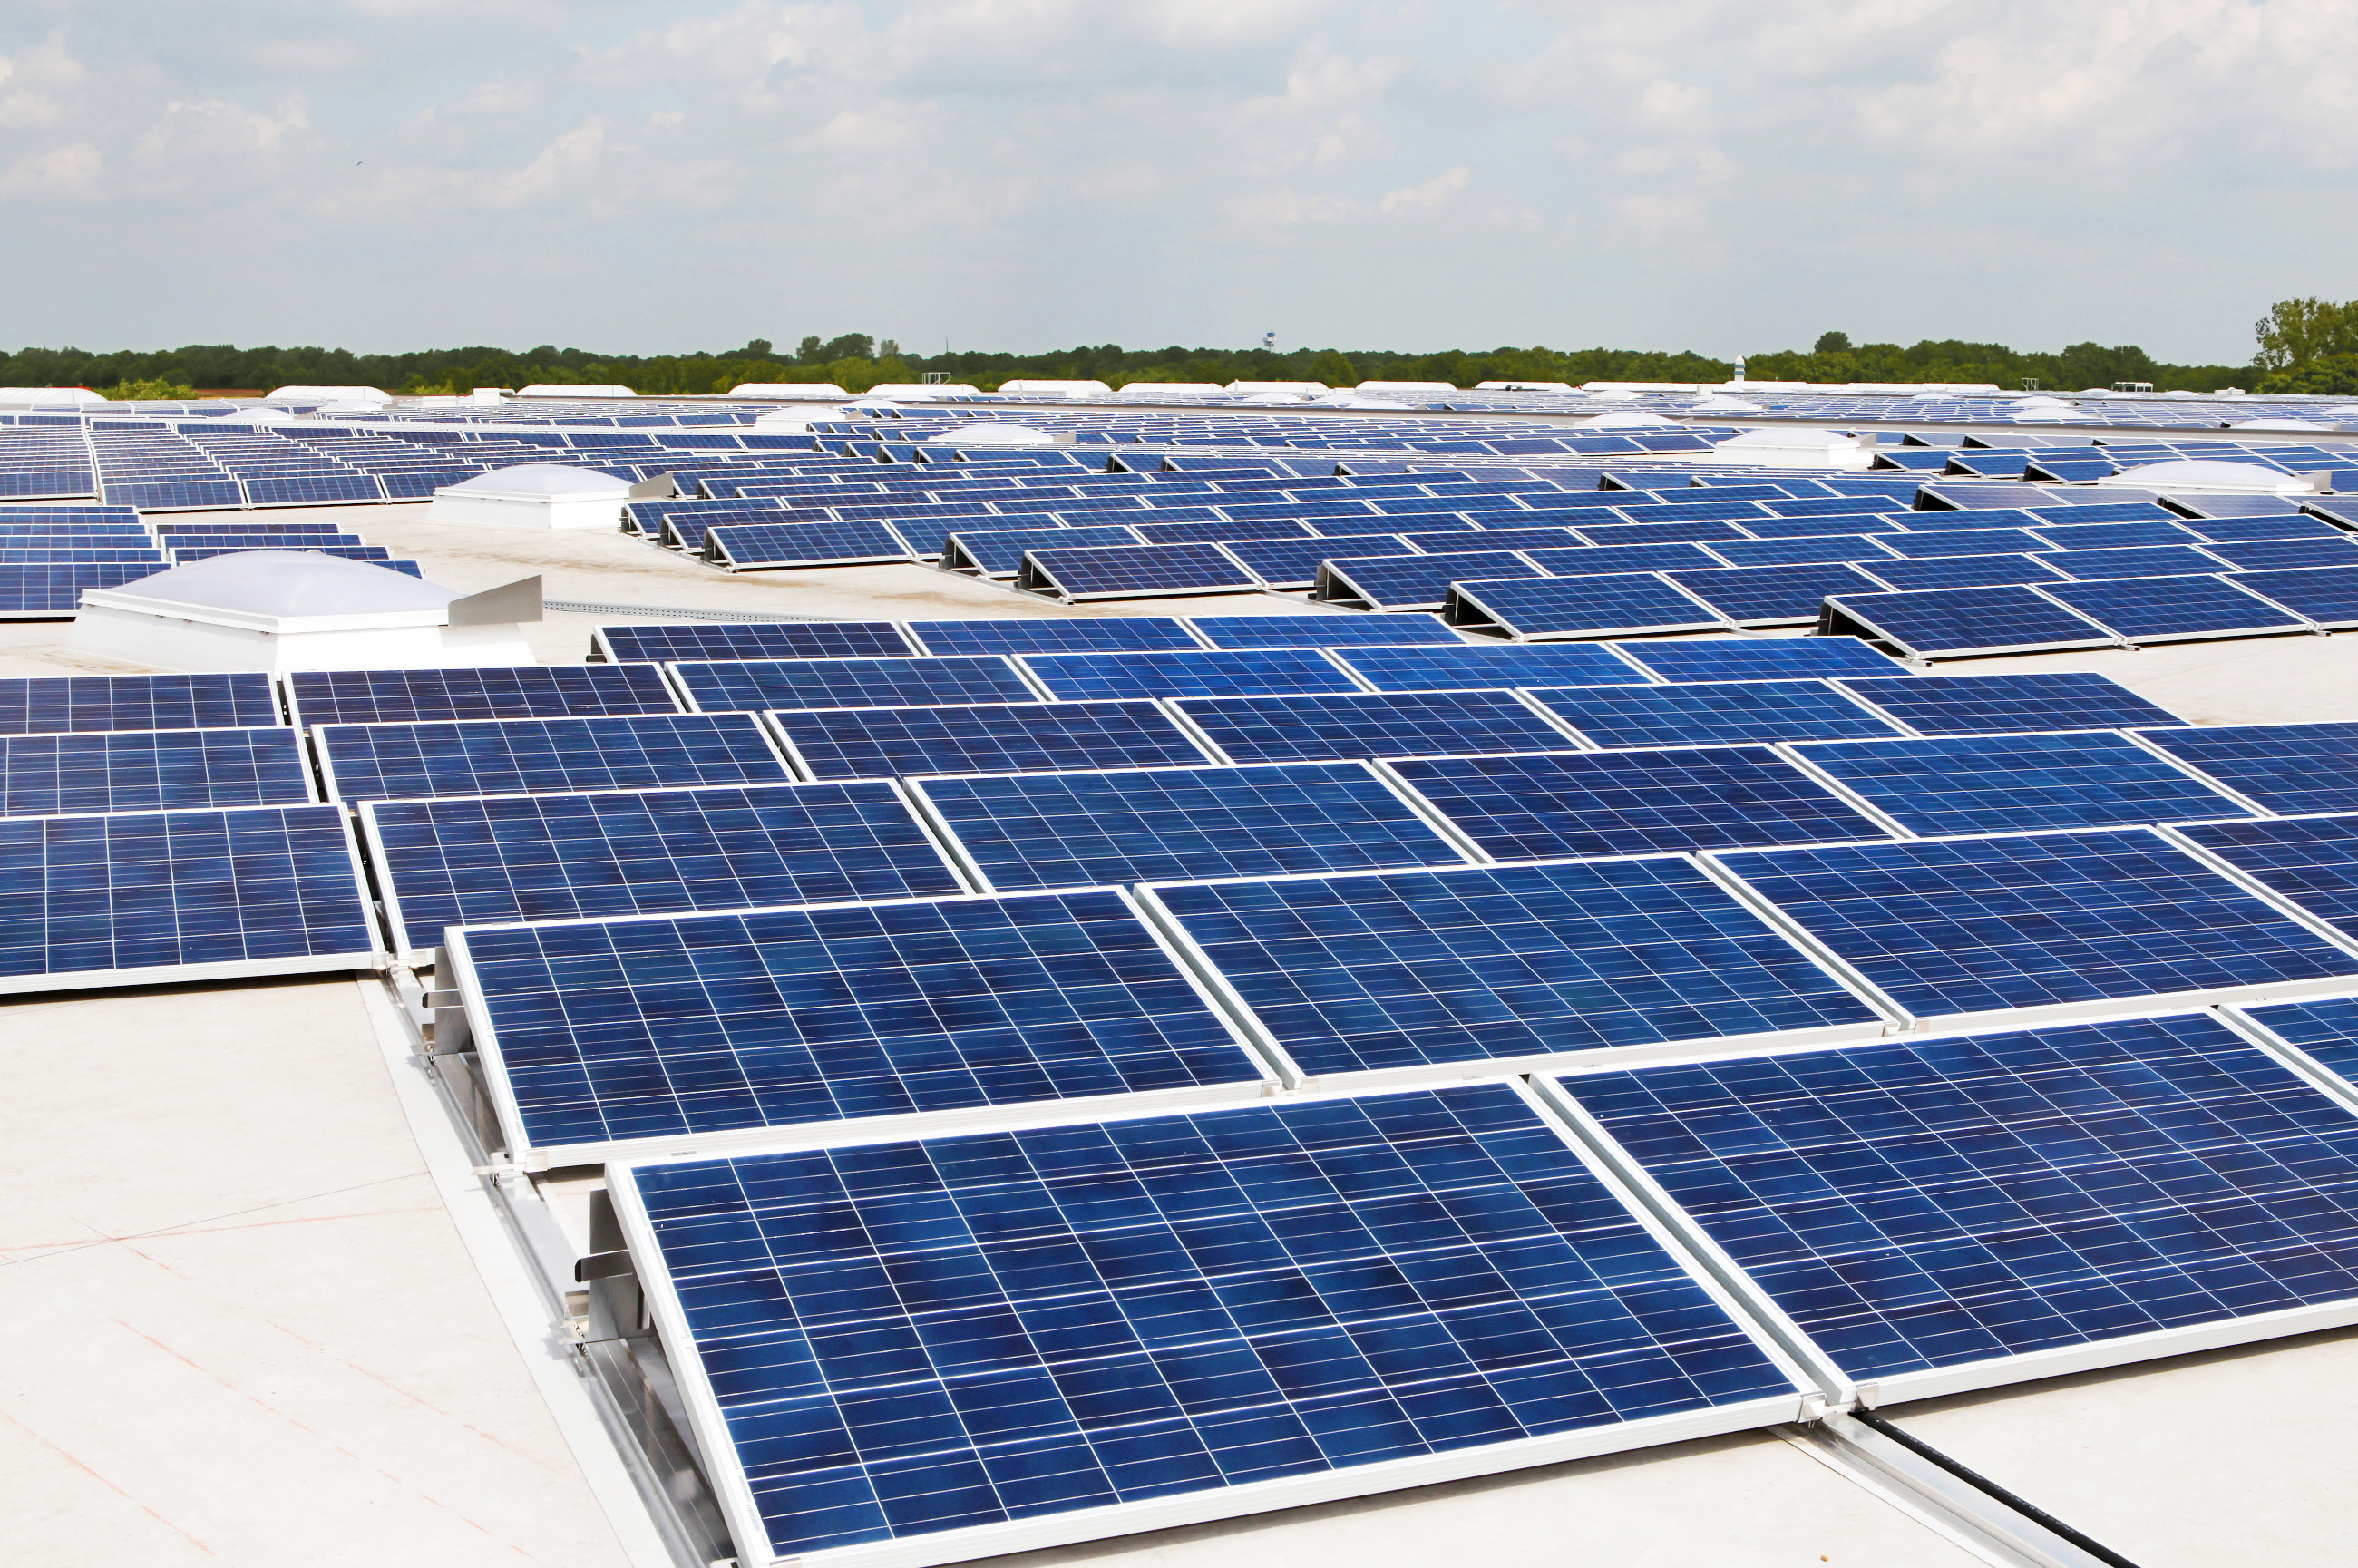
\includegraphics[width=\paperwidth,height=\paperheight]{images/titlepage/titlepic.jpg}%
        };

        % ------------------------------------------------ %
        % Info Table                                       %
        % ------------------------------------------------ %
        \node[%
            fill=black,
            fill opacity=0.75,
            rounded corners,
            outer sep=0pt,
            inner sep=1em,
            yshift=9em,
            anchor = south%
        ] at (current page.south) {\textcolor{white}{\infotable}};

        % ------------------------------------------------ %
        % FHNW Logo                                        %
        % ------------------------------------------------ %
        \node[anchor=north west,xshift=\logoX,yshift=-\logoY,outer sep=0pt,inner sep=0pt] at (current page.north west) {%
            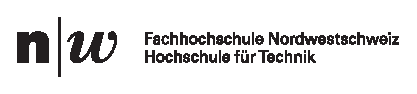
\includegraphics[height=12mm]{images/titlepage/fhnw.eps}%
        };
    \end{tikzpicture}



    % ---------------------------------------------------- %
    % The Text can  be set rather low in  the page without %
    % adjusting the top lengths.                           %
    % Backing up  and reseting these lengths  seems not to %
    % be necessary;  it appears  they are restored  at the %
    % end of the titlingpage environment.                  %
    % ---------------------------------------------------- %
    \setlength{\headsep}{0pt}
    \setlength{\headheight}{0pt}
    \setlength{\uppermargin}{4em}
    \checkandfixthelayout


    % ---------------------------------------------------- %
    % By   default,  centering   inside  the   titlingpage %
    % environment  will   center  with  respects   to  the %
    % typeblock. When  the  typeblock  is  centered,  this %
    % leads to  centered text  with respect to  the entire %
    % title  page. However,  When  the  typeblock  is  not %
    % centered, some adjustment is needed.                 %
    % See memman Chapter "Titles" for more information.    %
    % ---------------------------------------------------- %
    \calccentering{\unitlength}
    \begin{adjustwidth*}{\unitlength}{-\unitlength}


    % ---------------------------------------------------- %
    % Work some  magic to  automatically adjust  the hrule %
    % lengths to the length of the book title.             %
    %                                                      %
    % NOTE: The  font  size setting  needs  to  be in  the %
    % \mytitle  command, otherwise  \settolength will  not %
    % take it  into account  and will only  calculate with %
    % the default font size.                               %
    %                                                      %
    % NOTE  2: This mechanism  breaks if  the title  spans %
    % across multiple  lines. You're on  your own  in that %
    % case.                                                %
    % ---------------------------------------------------- %
    \newcommand{\mytitle}{{\textbf{\fontsize{25mm}{1em}\selectfont Project Powerline}}}
    \newlength{\titlelength}            % Length of title text
    \settowidth{\titlelength}{\mytitle}
    \newcommand{\titlerulefactor}{1.2}  % Length of title rules, as a factor

    % ---------------------------------------------------- %
    % Set the title color                                  %
    % ---------------------------------------------------- %
    \newcommand{\titlecolor}{black}

    % ---------------------------------------------------- %
    % Put the title onto the page                          %
    % ---------------------------------------------------- %
    \textcolor{\titlecolor}{%
        \centering
        \rule{\titlerulefactor\titlelength}{1pt} \\
        \vspace*{4mm}
        \mytitle\\
        %\vspace*{5mm}
        \rule{\titlerulefactor\titlelength}{1pt} \\
        \vspace*{6mm}
        \fontsize{8mm}{1em}\selectfont Fachbericht \\
    }


    % ---------------------------------------------------- %
    % This is the end of the centering magic.              %
    % ---------------------------------------------------- %
    \end{adjustwidth*}


    % ---------------------------------------------------- %
    % Make  sure  this  is   not  put  into  \frontmatter, %
    % otherwise it will get a \frontmatter folio.          %
    % \cleardoblepage  is not  actually necessary  because %
    % it  is  automatically   called  by  the  titlingpage %
    % environment.                                         %
    % ---------------------------------------------------- %
    %\cleardoublepage

    %\setlength{\headsep}{\originallength}
    %\checkandfixthelayout
\end{titlingpage}


% -------------------------------------------------------- %
% See  the  memoir  documentation  for  what  specifically %
% frontmatter does. Among  other things, page  numbers are %
% set to roman numerals and chapter numbers are removed.   %
% -------------------------------------------------------- %
\frontmatter

% -------------------------------------------------------- %
% Comment out what's not needed, obviously.                %
% -------------------------------------------------------- %
%\begin{centering}
\vspace*{30mm}
\begin{tiny}
    \begin{tabular}{lll}
        Inhalt & \copyright~2016 & Reto Nussbaumer   \\
               &                 &                   \\
        Design & \copyright~2016 & Raphael Frey      \\
    \end{tabular}


    % ---------------------------------------------------- %
    % Having  this  in  a  tabular  is  a  bit  ugly,  but %
    % it  ensures alignment  and  limited paragraph  width %
    % without much effort.                                 %
    % ---------------------------------------------------- %
    \vspace{1em}
    \begin{tabular}{p{.9\textwidth}}
        \noindent  Erstellt  im  Fr\"uhlingssemester 2016  an  der  Hochschule
        f\"ur  Technik  der  Fachhochschule   Nordwestschweiz  im  Rahmen  des
        Modules   \emph{Projekt  4}   des   Studiengangs  \emph{Elektro-   und
        Informationstechnologie}. \\

        \\
        \iftoggle{paper}{%
            Dies     ist    die     Druckversion    dieses     Dokuments. Eine
            elektronische     Version      mit     farbig     hervorgehobenen,
            klickbaren   Links   ist   auf  den   abgegebenen   elektronischen
            Datentr\"agern  in  Anhang \ref{app:electronicStorage}  auf  Seite
            \pageref{app:electronicStorage}   zu   finden    oder   kann   bei
            \code{raphael.frey@students.fhnw.ch} angefordert werden.
        }{%
            Dies ist die elektronische  Ausf\"uhrung des Dokuments. Links sind
            farbig hervorgehoben und klickbar. Falls eine Version ohne farbige
            Akzentuierung erw\"unscht ist, kann diese bei
            \href{mailto:raphael.frey@students.fhnw.ch}{\code{raphael.frey@students.fhnw.ch}}
            angefordert werden.
            % internet links: blau
            % externe links: magenta
        }
        \\

        \\
        Dieses Dokument hat bisher \thecounttexruns~Kompiliervorg\"ange durchlaufen. \\
    \end{tabular}
    \vspace{1em}

    \begin{tabular}{>{\ttfamily}lrl}
        Version 1 & 16.06.2016 & Abgabe \\
    \end{tabular}

    \vspace{1em}
    \begin{tabular}{l @{${}:{}$} l}
        Quelle Titelbild & \cite{ref:titlepage:pvanlage} \\
        Quelle Logo FHNW & \cite{ref:fhnwlogo}           \\
    \end{tabular}
\end{tiny}
%\\
%\footnotesize{\checkmark~\np~\noi~\partially} \\
%\\
%\large{\checkmark~\np~\noi~\partially} \\
%\\
%\checkmark~\np~\noi~\partially
%\end{centering}

% **************************************************************************** %
\chapter*{Abstract}
\label{chap:abstract}
% **************************************************************************** %

\emph{Note: I have  added headings  for the five  sections of  the ``abstract
hand'' to  highlight my thinking process;  obviously those will be  removed in
the final version.}

\vspace{2em}
\textbf{Research Question: What does the client expect?}\\
This  project's aim  was  to  develop a  system  for  real-time monitoring  of
photovoltaic  facilities on  the level  of single  panels. The system  must be
cost-effective and should scale from small single-household solutions to large
industrial-scale solar farms. Panels which are  not operating at full capacity
for whatever reason  (dirt, shade, defects) must be detected  and announced to
the user so that appropriate measures (cleaning, replacement) can be taken.

\textbf{Relevance}\\
Monitoring individual photovoltaic modules  will allow the facility's operator
to run  their solar farm at  optimal conditions, thus reducing  losses in both
power output and money.

\textbf{Background}\\
Current solutions for per-module monitoring  of solar facilities are expensive
and are  therefore often  foregone in  order to save  costs when  building new
facilities. This approach is short-sighted and more expensive in the long term
because not being able  to properly monitor a solar facility  means that it is
often not operating at optimal  conditions. As non-renewable sources of energy
such  as fossil  fuels  and nuclear  power are  losing  ground to  alternative
sources of  energy such  as wind and  solar power, the  overall losses  in the
energy industry of power and money  incurred due to insufficient monitoring of
solar facilities will become unsustainable.

\textbf{Method}\\
Our  system consists  of  two primary  components: A  controller is  installed
centrally  near  the  inverter. Additionally,  a sensor  is  mounted  on  each
photovoltaic  panel.  Communication  between  the sensors  and  the master  is
routed  through the  direct  current power  transmission  line; no  additional
wiring is needed. A  coil is used to  couple the signal to  the power line. In
case  of  an  error (e.g.  a  dirty  panel),  a  text  message is  sent  to  a
user-configurable phone  number. Additionally, local alarms such  as sirens or
warning lights  can be connected  to our system  and are triggered  whenever a
text message is sent.

\textbf{Results}\\
Simulations for  various coupling methods  for a string  of 20 PV  panels have
been performed. Inductive  coupling at  non-resonance conditions results  in a
signal  level  of roughly  \SI{6}{\milli\volt}  peak-to-peak  at the  receiver
without  amplification. Operating  the  circuit  at resonance  yields  a  much
improved peak-to-peak  voltage of \SI{250}{\milli\volt} at  the receiver (also
without amplification), which is sufficient for our purposes.

A  frequency sweep  for  the coupling  coil has  been  measured and  inductive
behavior up to  \SI{20}{\mega\hertz} verified, thus ensuring that  the coil we
have  picked is  suitable for  our uses  and  allows the  of a  vast range  of
frequencies as  needed. The system can  therefore adapt to conditions  in each
specific setup.

\vspace{1em}
\emph{Question: How negative  should we  go in  the paragraph  below? We don't
exactly  want to  sound like  depressed failures,  but then  again, facts  are
facts, and things  just aren't working properly. Should we  also add something
about how  we would proceed if  we had the time  or is this not  the place for
that?}

\vspace{1em}
The system  in its  entirety is  at this  point not  operational. The sensor's
components  do not  yet  work perfectly  in unison;  error  analysis is  still
ongoing. The printed circuit board for the  master device is not available due
to an issue with the  manufacturer when ordering. However, development for the
master's software is mostly completed.  A functioning graphical user interface
has been implemented and a database to which it connects is functional.

\vspace{2em}
\textbf{Key  words:}  photovoltaic  technology,  photovoltaic  module,  remote
monitoring, solar technology, PV cell, power efficiency, alternative energy,
powerline, communication, inductive coupling, capacitive coupling

%\include{frontmatter/dedication}
%\include{frontmatter/declaration}
%\include{frontmatter/acknowledgements}


% -------------------------------------------------------- %
% The starred versions do not make an entry for themselves %
% in the ToC, the unstarred versions do.                   %
% -------------------------------------------------------- %
\tableofcontents*
%\listoffigures
%\listoftables


% -------------------------------------------------------- %
% Set page numbers to  arabic numerals, reset page counter %
% to 1, display  chapter numbers. See memoir documentation %
% for more information.                                    %
% -------------------------------------------------------- %
\mainmatter


% -------------------------------------------------------- %
% It is  advisable to use actually  meaningful chapter and %
% section names instead of generically numbered ones as in %
% this  example structure. That  way, their  place in  the %
% document is not directly tied to their file name, and it %
% is  possible to  restructure the  document (e.g.  move a %
% section  from one  chapter  to another,  or reorder  the %
% chapters)  without  needing  to adjust  file  names  and %
% similar shenanigans.                                     %
% -------------------------------------------------------- %
% **************************************************************************** %
\chapter{Einleitung}
\label{chap:einleitung}
% **************************************************************************** %

Photovoltaikanlagen   sind  heutzutage   kein   Nischenprodukt  mehr. Um   die
Abhängigkeit  vom Erdöl  zu verringern,  werden vielerorts  kleine, aber  auch
grosse  Anlagen gebaut. Die  W\"arme-Energie, welche  kostenlos von  der Sonne
kommt,  wird  in elektrische  Energie  umgewandelt  und  kann gleich  vor  Ort
genutzt werden. Anlagenbesitzer  investieren meistens einen grossen  Betrag in
eine  neue  Anlage  und  sind  darauf angewiesen,  dass  diese  den  maximalen
Ertrag  liefert. Das ist  in der  Regel  ohne grossen  Aufwand der  Fall. Doch
es  gibt Umstände,  welche  die Effizienz  einer Photovoltaikanlage  erheblich
verringern  können und  dies meist  ohne, dass  es jemand  bemerkt.  In  einer
Photovoltaikanlage  werden üblicherweise  mehrere  PV-Module  zu einem  String
zusammengefasst,  indem  sie  in   Serie  geschaltet  werden. Dabei  kann  ein
abgeschattetes,  verschmutztes  oder  gar  defektes  Modul  den  Strom  dieser
Serieschaltung und somit auch die Leistung des gesamten Strings und der Anlage
stark beeinträchtigen. Was grosse finanzielle Einbussen zur Folge haben kann.

Das  Ziel des  Projektes P4  war es,  ein PV-Überwachungssystem  bestehend aus
einer Sensorplatine für den Einbau in  die Anschlussbox jedes Moduls und einem
zentralen Meldegerät  für den Einbau  im Schaltschrank beim  Wechselrichter zu
entwickeln, aufzubauen und zu testen. Die  Sensorplatine soll die Spannung des
jeweiligen PV-Modules  messen und sie  an das Mastergerät über  die bestehende
DC-Leitung  der  Anlage  übermitteln. Im  Mastergerät  werden  die  gemessenen
Spannungen der  einzelnen PV-Module  gespeichert und  ausgewertet. Erkennt das
Mastergerät ein fehlerhaftes  PV-Modul, soll eine Alarmierung  am Gerät selbst
und  per  SMS  ausgegeben  werden. Zusätzlich wird  ein  Relais  zur  externen
Signalisation  betätigt.   Das  System  soll  möglichst  energieeffizient  und
kostengünstig sein,  um die wirtschaftlichkeit einer  Photovoltaikanlage nicht
zu verschlechtern.

Das  Hauptproblem liegt  bei  der Signalübertragung  über  die DC-Leitung  der
Photovoltaikanlage. Denn die Spannung darauf schwankt  zwischen 12 und 60 Volt
an der Sensorplatine  und beträgt am Mastergerät bis zu  1000 Volt. Auf dieser
Leitung  ein Signal  zu  übertragen  ist schwierig  und  wird heutzutage  kaum
gemacht.  Zudem muss auf kleine Leistung beim gesamten System geachtet werden,
um keine wertfolle Energie zu verschwenden.

\todo{Beschreibung unseres Produkts}

Der vorliegende  Bericht stellt  die technische Dokumentation  unseres Systems
dar.  Zuerst wird das Konzept unserer L\"osung beschrieben, zusammen mit einer
Benutzerf\"uhrung.  Anschliessend  wird auf  das Hardware-  und Firmwaredesign
eingegangen,  und   zuletzt  werden  die  am   System  durchgef\"uhrten  Tests
dokumentiert.

\lipsum

% **************************************************************************** %
\chapter{\"Uberblick}
\label{chap:uberblick}
% **************************************************************************** %
Dieses Kapitel  beschreibt zuerst die grobe  Idee unsers L\"osungskonzepts. Es
wird  dargelegt, wie  unser System  in  eine Solaranlage  (bestehend oder  neu
aufgebaut) integriert wird, wie das System mit seiner Umgebung interagiert und
wie es zu bedienen ist.


% ---------------------------------------------------------------------------- %
\section{Aufbau einer Solaranlage}
\label{sec:solaranlage:aufbau}
% ---------------------------------------------------------------------------- %

Grunds\"atzlicher Aufbau einer Solaranlage: Zelle -> Modul -> Strings -> Anlage


% ---------------------------------------------------------------------------- %
\section{Einbettung in Umwelt}
\label{sec:einbettung}
% ---------------------------------------------------------------------------- %

Hier  wird  beschrieben,  wie  unser System  physisch  mit  einer  Solaranlage
integriert wird und welche Schnittstellen es zu welchem Zweck zur Anlage hat.
\todo{kein eigener Abschnitt mehr n\"otig}

% ---------------------------------------------------------------------------- %
\clearpage
\section{Abgeschattete Solarzellen}
\label{sec:shadedCells}
% ---------------------------------------------------------------------------- %

\todo{Referenzen auf Simu-Circuits}

% ---------------------------------------------------------------------------- %
% Performance Calculations
%
% Based on:
%http://tex.stackexchange.com/questions/185488/pgfplots-read-data-calculate-diagram#186016
% ---------------------------------------------------------------------------- %

%\pgfplotstableread{data/iv-curves/module-72cells-series--reference--all-ok.dat}\cellsAllOK
%\pgfplotstableset{
%    create on use/power output/.style={
%        create col/expr={\thisrow{V(out)} * \thisrow{I(R_load)}}
%    }
%}
%\pgfplotstableread{data/iv-curves/module-72cells-series--reference--ifail-5A.dat}\cellsFiveA
%\pgfplotstableset{
%    create on use/power output/.style={
%        create col/expr={\thisrow{V(out)} * \thisrow{I(R_load)}}
%    }
%}
%
%\pgfplotstableread{data/iv-curves/module-72cells-series--reference--ifail-1A.dat}\cellsOneA
%\pgfplotstableset{
%    create on use/power output/.style={
%        create col/expr={\thisrow{V(out)} * \thisrow{I(R_load)}}
%    }
%}
%
%\pgfplotstableread{data/iv-curves/module-string-complete--all-ok.dat}\moduleAllOK
%\pgfplotstableset{
%    create on use/power output/.style={
%        create col/expr={\thisrow{V(out)} * \thisrow{I(R_load)}}
%    }
%}
%\pgfplotstableread{data/iv-curves/module-string-complete--ifail-5A.dat}\moduleFiveA
%\pgfplotstableset{
%    create on use/power output/.style={
%        create col/expr={\thisrow{V(out)} * \thisrow{I(R_load)}}
%    }
%}
%\pgfplotstableread{data/iv-curves/module-string-complete--ifail-1A.dat}\moduleOneA
%\pgfplotstableset{
%    create on use/power output/.style={
%        create col/expr={\thisrow{V(out)} * \thisrow{I(R_load)}}
%    }
%}
%% END Performance Calculations ----------------------------------------------- %
%
%\begin{figure}[h!tb]
%    \begin{tikzpicture}
%       \begin{scope}[x={(0mm,0mm)},y={(90mm,\textwidth)}]
%           \begin{axis}[%
%                   height=50mm,
%                   width=\textwidth,
%                   at={(0,50mm)},
%                   grid=both,
%                   xlabel=Spannung (\si{\volt}),
%                   ylabel=Strom (\si{\ampere}),
%                   %axis y line*=left,
%                   %x unit=u,
%                   %change x base=true,
%                   %line width = 1pt,
%                   %thick,
%                   %x SI prefix=micro,
%               ]
%                \addplot[-,color=blue] table {data/iv-curves/module-72cells-series--reference--all-ok.dat};
%                \addplot[-,color=teal] table {data/iv-curves/module-72cells-series--reference--ifail-5A.dat};
%                \addplot[-,color=magenta] table {data/iv-curves/module-72cells-series--reference--ifail-1A.dat};
%            \end{axis}
%            \begin{axis}[%
%                   height=50mm,
%                   width=\textwidth,
%                   at={(0,0)},
%                   grid=both,
%                   xlabel=Spannung (\si{\volt}),
%                   ylabel=Leistung (\si{\watt}),
%                   %axis y line*=left,
%                   %x unit=u,
%                   %change x base=true,
%                   %line width = 1pt,
%                   %thick,
%                   %x SI prefix=micro,
%               ]
%                \addplot [blue] table [y=power output] {\cellsAllOK} node {};
%                \addplot [teal] table [y=power output] {\cellsFiveA} node {};
%                \addplot [magenta] table [y=power output] {\cellsOneA} node {};
%            \end{axis}
%        \end{scope}
%    \end{tikzpicture}
%    \caption{%
%        Oberes Diagramm: Simulierte  Strom-Spannungs-Kurve eines Moduls  aus 72
%        Zellen (in Serie geschaltet) mit einer degradierten Zelle\protect\\
%        Unteres Diagramm: Die zum oberen Diagramm geh\"orenden Leistungskurven.
%        Gut erkennbar  ist, dass  selbst bei nur  einer degradierten  Zelle die
%        verf\"ugbare Leistung des gesamten Moduls stark abnimmt.\protect\\
%        \textbf{\textcolor{blue}{blau}}: Alle   Zellen  geben   volle  Leistung
%        ab.\protect\\
%        \textbf{\textcolor{teal}{blaugr\"un}}: Eine Zelle  von 72 gibt  nur den
%        halben Strom ab.\protect\\
%        \textbf{\textcolor{magenta}{magenta}}: Eine  Zelle  gibt nur  10\%  des
%        vollen Stromes ab.\protect\\
%        Die zuge\"orige \code{LTspice}-Schaltung basiert  auf dem Modell eines
%        Moduls aus Abbildung \ref{fig:ltspice:module:cellBased:72x1} auf Seite
%        \pageref{fig:ltspice:module:cellBased:72x1} im Anhang. Dabei wurde die
%        Stromquelle  in  einer  Zelle  variiert  (100\%,  50\%  bzw. 10\%  der
%        restlichen Quellen).%
%    }
%    \label{fig:ivcurve:cells}
%\end{figure}
%\begin{figure}[h!tb]
%    \begin{tikzpicture}
%       \begin{scope}[x={(0mm,0mm)},y={(100mm,\textwidth)}]
%           \begin{axis}[%
%                   height=50mm,
%                   width=\textwidth,
%                   at={(0,50mm)},
%                   grid=both,
%                   xlabel=Spannung (\si{\volt}),
%                   ylabel=Strom (\si{\ampere}),
%                   %x unit=u,
%                   %change x base=true,
%                   %line width = 1pt,
%                   %thick,
%                   %x SI prefix=micro,
%               ]
%                \addplot[-,color=blue] table {data/iv-curves/module-string-complete--all-ok.dat};
%                \addplot[-,color=magenta] table {data/iv-curves/module-string-complete--ifail-1A.dat};
%                \addplot[-,color=teal] table {data/iv-curves/module-string-complete--ifail-5A.dat};
%            \end{axis}
%            \begin{axis}[%
%                   height=50mm,
%                   width=\textwidth,
%                   at={(0,0)},
%                   grid=both,
%                   xlabel=Spannung (\si{\volt}),
%                   ylabel=Leistung (\si{\watt}),
%                   %axis y line*=left,
%                   %x unit=u,
%                   %change x base=true,
%                   %line width = 1pt,
%                   %thick,
%                   %x SI prefix=micro,
%               ]
%                \addplot [blue] table [y=power output] {\moduleAllOK} node {};
%                \addplot [teal] table [y=power output] {\moduleFiveA} node {};
%                \addplot [magenta] table [y=power output] {\moduleOneA} node {};
%            \end{axis}
%        \end{scope}
%    \end{tikzpicture}
%   \caption{%
%       Oberes  Diagramm: Simulierte  Strom-Spannungs-Kurve eines  Strangs  von
%       Modulen mit  einem degradierten Modul.\protect\\  Unteres Diagramm: Die
%       zum oberen Diagramm geh\"orenden Leistungskurven.  Selbst ein einzelnes
%       degradiertes  Modul  f\"uhrt  zu  einem  bedeutenden  Leistungseinbruch
%       des  gesamten  Modulstrangs.   Verkn\"upft  man  diese  Erkenntnis  mit
%       den Informationen  aus Abbildung \ref{fig:ivcurve:cells},  l\"asst sich
%       folgern, dass  lediglich eine  einzelne degradierte Zelle  von mehreren
%       hundert in  einem Modulstrang  vorhandenen Zellen  die gesamte  auf dem
%       Strang verf\"ugbare Leistung massiv senken kann.\protect\\
%       \textbf{\textcolor{blue}{blau}}: Alle   Module   geben   vollen   Strom
%       ab.\protect\\
%       \textbf{\textcolor{teal}{blaugr\"un}}: Ein Modul  von zwanzig  gibt nur
%       den halben Strom ab.\protect\\
%       \textbf{\textcolor{magenta}{magenta}}: Ein  Modul  gibt  nur  10\%  des
%       vollen Stromes ab.\protect\\
%       Die       zuge\"orige       \code{LTspice}-Schaltung       ist       in
%       Abbildung    \ref{fig:ltspice:vicurvesimulator:modules}    auf    Seite
%       \pageref{fig:ltspice:vicurvesimulator:modules} im Anhang zu finden.%
%   }
%   \label{fig:ivcurve:modules}
%\end{figure}

% ---------------------------------------------------------------------------- %
\clearpage
\section{Kommunikation \"uber DC-Leitung}
\label{sec:commDCLine}
% ---------------------------------------------------------------------------- %

Die Kommunikation zwischen  \Sensor und \Master \"uber die  DC-Leitung ist das
Herzst\"uck des Systems und das zu l\"osende Kernproblem des Projekts. Es sind
im Rahmen  des Projekts  zwei grunds\"atzliche  Ans\"atze verfolgt  worden, um
Daten  zwischen  \Sensor und  \Master  \"uber  die  DC-Leitung zu  senden  und
empfangen.

\textbf{Frequency-shift keying}: Bei  der FSK (Frequenzumtastung  auf Deutsch)
wird  dem in  der Leitung  fliessenden Gleichstrom  ein (verh\"altnism\"assig)
kleines  Signal aufmoduliert,  welches  die  zu \"ubertragenden  Informationen
enth\"alt. Die  Frequenz   des  aufmodulierten   Anteils  wird   in  diskreten
Schritten variiert  und jeweils  einem Symbol zugeordnet. Bei  einer bin\"aren
Umsetzung  werden  zwei  Frequenzen  benutzt; eine  f\"ur  \code{0}  und  eine
f\"ur  \code{1}.   Das  Verfahren ist  schematisch  in  \fref{fig:fsk:concept}
dargestellt.

\begin{figure}[h!tb]
    \centering
    %% Creator: Matplotlib, PGF backend
%%
%% To include the figure in your LaTeX document, write
%%   \input{<filename>.pgf}
%%
%% Make sure the required packages are loaded in your preamble
%%   \usepackage{pgf}
%%
%% Figures using additional raster images can only be included by \input if
%% they are in the same directory as the main LaTeX file. For loading figures
%% from other directories you can use the `import` package
%%   \usepackage{import}
%% and then include the figures with
%%   \import{<path to file>}{<filename>.pgf}
%%
%% Matplotlib used the following preamble
%%   \usepackage{fontspec}
%%   \setmainfont{Bitstream Vera Serif}
%%   \setsansfont{Bitstream Vera Sans}
%%   \setmonofont{Bitstream Vera Sans Mono}
%%
\begingroup%
\makeatletter%
\begin{pgfpicture}%
\pgfpathrectangle{\pgfpointorigin}{\pgfqpoint{5.000000in}{3.500000in}}%
\pgfusepath{use as bounding box, clip}%
\begin{pgfscope}%
\pgfsetbuttcap%
\pgfsetmiterjoin%
\pgfsetlinewidth{0.000000pt}%
\definecolor{currentstroke}{rgb}{0.000000,0.000000,0.000000}%
\pgfsetstrokecolor{currentstroke}%
\pgfsetstrokeopacity{0.000000}%
\pgfsetdash{}{0pt}%
\pgfpathmoveto{\pgfqpoint{0.000000in}{0.000000in}}%
\pgfpathlineto{\pgfqpoint{5.000000in}{0.000000in}}%
\pgfpathlineto{\pgfqpoint{5.000000in}{3.500000in}}%
\pgfpathlineto{\pgfqpoint{0.000000in}{3.500000in}}%
\pgfpathclose%
\pgfusepath{}%
\end{pgfscope}%
\begin{pgfscope}%
\pgfsetbuttcap%
\pgfsetmiterjoin%
\pgfsetlinewidth{0.000000pt}%
\definecolor{currentstroke}{rgb}{0.000000,0.000000,0.000000}%
\pgfsetstrokecolor{currentstroke}%
\pgfsetstrokeopacity{0.000000}%
\pgfsetdash{}{0pt}%
\pgfpathmoveto{\pgfqpoint{0.750000in}{2.268396in}}%
\pgfpathlineto{\pgfqpoint{4.750000in}{2.268396in}}%
\pgfpathlineto{\pgfqpoint{4.750000in}{3.325000in}}%
\pgfpathlineto{\pgfqpoint{0.750000in}{3.325000in}}%
\pgfpathclose%
\pgfusepath{}%
\end{pgfscope}%
\begin{pgfscope}%
\pgfpathrectangle{\pgfqpoint{0.750000in}{2.268396in}}{\pgfqpoint{4.000000in}{1.056604in}} %
\pgfusepath{clip}%
\pgfsetrectcap%
\pgfsetroundjoin%
\pgfsetlinewidth{0.501875pt}%
\definecolor{currentstroke}{rgb}{0.000000,0.000000,1.000000}%
\pgfsetstrokecolor{currentstroke}%
\pgfsetdash{}{0pt}%
\pgfpathmoveto{\pgfqpoint{0.750000in}{2.356447in}}%
\pgfpathlineto{\pgfqpoint{1.701998in}{2.356447in}}%
\pgfusepath{stroke}%
\end{pgfscope}%
\begin{pgfscope}%
\pgfpathrectangle{\pgfqpoint{0.750000in}{2.268396in}}{\pgfqpoint{4.000000in}{1.056604in}} %
\pgfusepath{clip}%
\pgfsetrectcap%
\pgfsetroundjoin%
\pgfsetlinewidth{0.501875pt}%
\definecolor{currentstroke}{rgb}{0.501961,0.501961,0.501961}%
\pgfsetstrokecolor{currentstroke}%
\pgfsetdash{}{0pt}%
\pgfpathmoveto{\pgfqpoint{1.701998in}{2.356447in}}%
\pgfpathlineto{\pgfqpoint{1.701998in}{3.236950in}}%
\pgfusepath{stroke}%
\end{pgfscope}%
\begin{pgfscope}%
\pgfpathrectangle{\pgfqpoint{0.750000in}{2.268396in}}{\pgfqpoint{4.000000in}{1.056604in}} %
\pgfusepath{clip}%
\pgfsetrectcap%
\pgfsetroundjoin%
\pgfsetlinewidth{0.501875pt}%
\definecolor{currentstroke}{rgb}{1.000000,0.000000,1.000000}%
\pgfsetstrokecolor{currentstroke}%
\pgfsetdash{}{0pt}%
\pgfpathmoveto{\pgfqpoint{1.701998in}{3.236950in}}%
\pgfpathlineto{\pgfqpoint{2.653996in}{3.236950in}}%
\pgfusepath{stroke}%
\end{pgfscope}%
\begin{pgfscope}%
\pgfpathrectangle{\pgfqpoint{0.750000in}{2.268396in}}{\pgfqpoint{4.000000in}{1.056604in}} %
\pgfusepath{clip}%
\pgfsetrectcap%
\pgfsetroundjoin%
\pgfsetlinewidth{0.501875pt}%
\definecolor{currentstroke}{rgb}{0.501961,0.501961,0.501961}%
\pgfsetstrokecolor{currentstroke}%
\pgfsetdash{}{0pt}%
\pgfpathmoveto{\pgfqpoint{2.653996in}{3.236950in}}%
\pgfpathlineto{\pgfqpoint{2.653996in}{2.356447in}}%
\pgfusepath{stroke}%
\end{pgfscope}%
\begin{pgfscope}%
\pgfpathrectangle{\pgfqpoint{0.750000in}{2.268396in}}{\pgfqpoint{4.000000in}{1.056604in}} %
\pgfusepath{clip}%
\pgfsetrectcap%
\pgfsetroundjoin%
\pgfsetlinewidth{0.501875pt}%
\definecolor{currentstroke}{rgb}{0.000000,0.000000,1.000000}%
\pgfsetstrokecolor{currentstroke}%
\pgfsetdash{}{0pt}%
\pgfpathmoveto{\pgfqpoint{2.653996in}{2.356447in}}%
\pgfpathlineto{\pgfqpoint{3.605993in}{2.356447in}}%
\pgfusepath{stroke}%
\end{pgfscope}%
\begin{pgfscope}%
\pgfpathrectangle{\pgfqpoint{0.750000in}{2.268396in}}{\pgfqpoint{4.000000in}{1.056604in}} %
\pgfusepath{clip}%
\pgfsetrectcap%
\pgfsetroundjoin%
\pgfsetlinewidth{0.501875pt}%
\definecolor{currentstroke}{rgb}{0.501961,0.501961,0.501961}%
\pgfsetstrokecolor{currentstroke}%
\pgfsetdash{}{0pt}%
\pgfpathmoveto{\pgfqpoint{3.605993in}{2.356447in}}%
\pgfpathlineto{\pgfqpoint{3.605993in}{3.236950in}}%
\pgfusepath{stroke}%
\end{pgfscope}%
\begin{pgfscope}%
\pgfpathrectangle{\pgfqpoint{0.750000in}{2.268396in}}{\pgfqpoint{4.000000in}{1.056604in}} %
\pgfusepath{clip}%
\pgfsetrectcap%
\pgfsetroundjoin%
\pgfsetlinewidth{0.501875pt}%
\definecolor{currentstroke}{rgb}{1.000000,0.000000,1.000000}%
\pgfsetstrokecolor{currentstroke}%
\pgfsetdash{}{0pt}%
\pgfpathmoveto{\pgfqpoint{3.605993in}{3.236950in}}%
\pgfpathlineto{\pgfqpoint{4.557991in}{3.236950in}}%
\pgfusepath{stroke}%
\end{pgfscope}%
\begin{pgfscope}%
\pgfsetrectcap%
\pgfsetmiterjoin%
\pgfsetlinewidth{0.501875pt}%
\definecolor{currentstroke}{rgb}{0.000000,0.000000,0.000000}%
\pgfsetstrokecolor{currentstroke}%
\pgfsetdash{}{0pt}%
\pgfpathmoveto{\pgfqpoint{4.750000in}{2.268396in}}%
\pgfpathlineto{\pgfqpoint{4.750000in}{3.325000in}}%
\pgfusepath{stroke}%
\end{pgfscope}%
\begin{pgfscope}%
\pgfsetrectcap%
\pgfsetmiterjoin%
\pgfsetlinewidth{0.501875pt}%
\definecolor{currentstroke}{rgb}{0.000000,0.000000,0.000000}%
\pgfsetstrokecolor{currentstroke}%
\pgfsetdash{}{0pt}%
\pgfpathmoveto{\pgfqpoint{0.750000in}{3.325000in}}%
\pgfpathlineto{\pgfqpoint{4.750000in}{3.325000in}}%
\pgfusepath{stroke}%
\end{pgfscope}%
\begin{pgfscope}%
\pgfsetrectcap%
\pgfsetmiterjoin%
\pgfsetlinewidth{0.501875pt}%
\definecolor{currentstroke}{rgb}{0.000000,0.000000,0.000000}%
\pgfsetstrokecolor{currentstroke}%
\pgfsetdash{}{0pt}%
\pgfpathmoveto{\pgfqpoint{0.750000in}{2.268396in}}%
\pgfpathlineto{\pgfqpoint{4.750000in}{2.268396in}}%
\pgfusepath{stroke}%
\end{pgfscope}%
\begin{pgfscope}%
\pgfsetrectcap%
\pgfsetmiterjoin%
\pgfsetlinewidth{0.501875pt}%
\definecolor{currentstroke}{rgb}{0.000000,0.000000,0.000000}%
\pgfsetstrokecolor{currentstroke}%
\pgfsetdash{}{0pt}%
\pgfpathmoveto{\pgfqpoint{0.750000in}{2.268396in}}%
\pgfpathlineto{\pgfqpoint{0.750000in}{3.325000in}}%
\pgfusepath{stroke}%
\end{pgfscope}%
\begin{pgfscope}%
\pgftext[x=2.750000in,y=2.198952in,,top]{\rmfamily\fontsize{9.000000}{10.800000}\selectfont Zeit}%
\end{pgfscope}%
\begin{pgfscope}%
\pgfsetbuttcap%
\pgfsetroundjoin%
\definecolor{currentfill}{rgb}{0.000000,0.000000,0.000000}%
\pgfsetfillcolor{currentfill}%
\pgfsetlinewidth{0.501875pt}%
\definecolor{currentstroke}{rgb}{0.000000,0.000000,0.000000}%
\pgfsetstrokecolor{currentstroke}%
\pgfsetdash{}{0pt}%
\pgfsys@defobject{currentmarker}{\pgfqpoint{0.000000in}{0.000000in}}{\pgfqpoint{0.055556in}{0.000000in}}{%
\pgfpathmoveto{\pgfqpoint{0.000000in}{0.000000in}}%
\pgfpathlineto{\pgfqpoint{0.055556in}{0.000000in}}%
\pgfusepath{stroke,fill}%
}%
\begin{pgfscope}%
\pgfsys@transformshift{0.750000in}{2.356447in}%
\pgfsys@useobject{currentmarker}{}%
\end{pgfscope}%
\end{pgfscope}%
\begin{pgfscope}%
\pgfsetbuttcap%
\pgfsetroundjoin%
\definecolor{currentfill}{rgb}{0.000000,0.000000,0.000000}%
\pgfsetfillcolor{currentfill}%
\pgfsetlinewidth{0.501875pt}%
\definecolor{currentstroke}{rgb}{0.000000,0.000000,0.000000}%
\pgfsetstrokecolor{currentstroke}%
\pgfsetdash{}{0pt}%
\pgfsys@defobject{currentmarker}{\pgfqpoint{-0.055556in}{0.000000in}}{\pgfqpoint{0.000000in}{0.000000in}}{%
\pgfpathmoveto{\pgfqpoint{0.000000in}{0.000000in}}%
\pgfpathlineto{\pgfqpoint{-0.055556in}{0.000000in}}%
\pgfusepath{stroke,fill}%
}%
\begin{pgfscope}%
\pgfsys@transformshift{4.750000in}{2.356447in}%
\pgfsys@useobject{currentmarker}{}%
\end{pgfscope}%
\end{pgfscope}%
\begin{pgfscope}%
\pgftext[x=0.694444in,y=2.356447in,right,]{\rmfamily\fontsize{9.000000}{10.800000}\selectfont \(\displaystyle 0\)}%
\end{pgfscope}%
\begin{pgfscope}%
\pgfsetbuttcap%
\pgfsetroundjoin%
\definecolor{currentfill}{rgb}{0.000000,0.000000,0.000000}%
\pgfsetfillcolor{currentfill}%
\pgfsetlinewidth{0.501875pt}%
\definecolor{currentstroke}{rgb}{0.000000,0.000000,0.000000}%
\pgfsetstrokecolor{currentstroke}%
\pgfsetdash{}{0pt}%
\pgfsys@defobject{currentmarker}{\pgfqpoint{0.000000in}{0.000000in}}{\pgfqpoint{0.055556in}{0.000000in}}{%
\pgfpathmoveto{\pgfqpoint{0.000000in}{0.000000in}}%
\pgfpathlineto{\pgfqpoint{0.055556in}{0.000000in}}%
\pgfusepath{stroke,fill}%
}%
\begin{pgfscope}%
\pgfsys@transformshift{0.750000in}{3.236950in}%
\pgfsys@useobject{currentmarker}{}%
\end{pgfscope}%
\end{pgfscope}%
\begin{pgfscope}%
\pgfsetbuttcap%
\pgfsetroundjoin%
\definecolor{currentfill}{rgb}{0.000000,0.000000,0.000000}%
\pgfsetfillcolor{currentfill}%
\pgfsetlinewidth{0.501875pt}%
\definecolor{currentstroke}{rgb}{0.000000,0.000000,0.000000}%
\pgfsetstrokecolor{currentstroke}%
\pgfsetdash{}{0pt}%
\pgfsys@defobject{currentmarker}{\pgfqpoint{-0.055556in}{0.000000in}}{\pgfqpoint{0.000000in}{0.000000in}}{%
\pgfpathmoveto{\pgfqpoint{0.000000in}{0.000000in}}%
\pgfpathlineto{\pgfqpoint{-0.055556in}{0.000000in}}%
\pgfusepath{stroke,fill}%
}%
\begin{pgfscope}%
\pgfsys@transformshift{4.750000in}{3.236950in}%
\pgfsys@useobject{currentmarker}{}%
\end{pgfscope}%
\end{pgfscope}%
\begin{pgfscope}%
\pgftext[x=0.694444in,y=3.236950in,right,]{\rmfamily\fontsize{9.000000}{10.800000}\selectfont \(\displaystyle 1\)}%
\end{pgfscope}%
\begin{pgfscope}%
\pgftext[x=0.560764in,y=2.796698in,,bottom,rotate=90.000000]{\rmfamily\fontsize{9.000000}{10.800000}\selectfont Symbol}%
\end{pgfscope}%
\begin{pgfscope}%
\pgftext[x=2.750000in,y=3.394444in,,base]{\rmfamily\fontsize{11.000000}{13.200000}\selectfont Daten}%
\end{pgfscope}%
\begin{pgfscope}%
\pgfsetbuttcap%
\pgfsetmiterjoin%
\pgfsetlinewidth{0.000000pt}%
\definecolor{currentstroke}{rgb}{0.000000,0.000000,0.000000}%
\pgfsetstrokecolor{currentstroke}%
\pgfsetstrokeopacity{0.000000}%
\pgfsetdash{}{0pt}%
\pgfpathmoveto{\pgfqpoint{0.750000in}{0.525000in}}%
\pgfpathlineto{\pgfqpoint{4.750000in}{0.525000in}}%
\pgfpathlineto{\pgfqpoint{4.750000in}{1.581604in}}%
\pgfpathlineto{\pgfqpoint{0.750000in}{1.581604in}}%
\pgfpathclose%
\pgfusepath{}%
\end{pgfscope}%
\begin{pgfscope}%
\pgfpathrectangle{\pgfqpoint{0.750000in}{0.525000in}}{\pgfqpoint{4.000000in}{1.056604in}} %
\pgfusepath{clip}%
\pgfsetrectcap%
\pgfsetroundjoin%
\pgfsetlinewidth{0.501875pt}%
\definecolor{currentstroke}{rgb}{0.000000,0.000000,1.000000}%
\pgfsetstrokecolor{currentstroke}%
\pgfsetdash{}{0pt}%
\pgfpathmoveto{\pgfqpoint{0.750000in}{0.573027in}}%
\pgfpathlineto{\pgfqpoint{0.754765in}{0.573977in}}%
\pgfpathlineto{\pgfqpoint{0.760482in}{0.577618in}}%
\pgfpathlineto{\pgfqpoint{0.766200in}{0.583967in}}%
\pgfpathlineto{\pgfqpoint{0.772871in}{0.594748in}}%
\pgfpathlineto{\pgfqpoint{0.780494in}{0.611414in}}%
\pgfpathlineto{\pgfqpoint{0.789071in}{0.635497in}}%
\pgfpathlineto{\pgfqpoint{0.799553in}{0.672160in}}%
\pgfpathlineto{\pgfqpoint{0.810989in}{0.720437in}}%
\pgfpathlineto{\pgfqpoint{0.825283in}{0.791283in}}%
\pgfpathlineto{\pgfqpoint{0.842436in}{0.888329in}}%
\pgfpathlineto{\pgfqpoint{0.869119in}{1.054057in}}%
\pgfpathlineto{\pgfqpoint{0.902472in}{1.258667in}}%
\pgfpathlineto{\pgfqpoint{0.919625in}{1.350889in}}%
\pgfpathlineto{\pgfqpoint{0.933919in}{1.416314in}}%
\pgfpathlineto{\pgfqpoint{0.946308in}{1.462665in}}%
\pgfpathlineto{\pgfqpoint{0.956790in}{1.493395in}}%
\pgfpathlineto{\pgfqpoint{0.965367in}{1.512303in}}%
\pgfpathlineto{\pgfqpoint{0.972990in}{1.524182in}}%
\pgfpathlineto{\pgfqpoint{0.979661in}{1.530670in}}%
\pgfpathlineto{\pgfqpoint{0.985379in}{1.533289in}}%
\pgfpathlineto{\pgfqpoint{0.990144in}{1.533384in}}%
\pgfpathlineto{\pgfqpoint{0.994908in}{1.531581in}}%
\pgfpathlineto{\pgfqpoint{1.000626in}{1.526921in}}%
\pgfpathlineto{\pgfqpoint{1.007297in}{1.518079in}}%
\pgfpathlineto{\pgfqpoint{1.014920in}{1.503570in}}%
\pgfpathlineto{\pgfqpoint{1.023497in}{1.481811in}}%
\pgfpathlineto{\pgfqpoint{1.033026in}{1.451214in}}%
\pgfpathlineto{\pgfqpoint{1.044462in}{1.406247in}}%
\pgfpathlineto{\pgfqpoint{1.057803in}{1.343724in}}%
\pgfpathlineto{\pgfqpoint{1.074003in}{1.255932in}}%
\pgfpathlineto{\pgfqpoint{1.095921in}{1.123283in}}%
\pgfpathlineto{\pgfqpoint{1.144522in}{0.825031in}}%
\pgfpathlineto{\pgfqpoint{1.160722in}{0.740557in}}%
\pgfpathlineto{\pgfqpoint{1.174063in}{0.681536in}}%
\pgfpathlineto{\pgfqpoint{1.185498in}{0.640040in}}%
\pgfpathlineto{\pgfqpoint{1.195981in}{0.610239in}}%
\pgfpathlineto{\pgfqpoint{1.204557in}{0.592135in}}%
\pgfpathlineto{\pgfqpoint{1.212181in}{0.580994in}}%
\pgfpathlineto{\pgfqpoint{1.218852in}{0.575163in}}%
\pgfpathlineto{\pgfqpoint{1.224569in}{0.573113in}}%
\pgfpathlineto{\pgfqpoint{1.229334in}{0.573493in}}%
\pgfpathlineto{\pgfqpoint{1.235052in}{0.576453in}}%
\pgfpathlineto{\pgfqpoint{1.240770in}{0.582127in}}%
\pgfpathlineto{\pgfqpoint{1.247440in}{0.592135in}}%
\pgfpathlineto{\pgfqpoint{1.255064in}{0.607943in}}%
\pgfpathlineto{\pgfqpoint{1.263640in}{0.631102in}}%
\pgfpathlineto{\pgfqpoint{1.274123in}{0.666714in}}%
\pgfpathlineto{\pgfqpoint{1.285558in}{0.713964in}}%
\pgfpathlineto{\pgfqpoint{1.298900in}{0.778756in}}%
\pgfpathlineto{\pgfqpoint{1.316053in}{0.874228in}}%
\pgfpathlineto{\pgfqpoint{1.340829in}{1.026884in}}%
\pgfpathlineto{\pgfqpoint{1.378947in}{1.261394in}}%
\pgfpathlineto{\pgfqpoint{1.396101in}{1.353254in}}%
\pgfpathlineto{\pgfqpoint{1.410395in}{1.418285in}}%
\pgfpathlineto{\pgfqpoint{1.421830in}{1.461077in}}%
\pgfpathlineto{\pgfqpoint{1.432313in}{1.492177in}}%
\pgfpathlineto{\pgfqpoint{1.440889in}{1.511404in}}%
\pgfpathlineto{\pgfqpoint{1.448513in}{1.523578in}}%
\pgfpathlineto{\pgfqpoint{1.455184in}{1.530329in}}%
\pgfpathlineto{\pgfqpoint{1.460901in}{1.533175in}}%
\pgfpathlineto{\pgfqpoint{1.465666in}{1.533460in}}%
\pgfpathlineto{\pgfqpoint{1.470431in}{1.531846in}}%
\pgfpathlineto{\pgfqpoint{1.476148in}{1.527413in}}%
\pgfpathlineto{\pgfqpoint{1.482819in}{1.518831in}}%
\pgfpathlineto{\pgfqpoint{1.490443in}{1.504612in}}%
\pgfpathlineto{\pgfqpoint{1.499019in}{1.483167in}}%
\pgfpathlineto{\pgfqpoint{1.508549in}{1.452898in}}%
\pgfpathlineto{\pgfqpoint{1.519984in}{1.408289in}}%
\pgfpathlineto{\pgfqpoint{1.533325in}{1.346124in}}%
\pgfpathlineto{\pgfqpoint{1.549526in}{1.258667in}}%
\pgfpathlineto{\pgfqpoint{1.571444in}{1.126270in}}%
\pgfpathlineto{\pgfqpoint{1.620997in}{0.822378in}}%
\pgfpathlineto{\pgfqpoint{1.637197in}{0.738270in}}%
\pgfpathlineto{\pgfqpoint{1.650538in}{0.679631in}}%
\pgfpathlineto{\pgfqpoint{1.661974in}{0.638509in}}%
\pgfpathlineto{\pgfqpoint{1.671503in}{0.611414in}}%
\pgfpathlineto{\pgfqpoint{1.680080in}{0.592988in}}%
\pgfpathlineto{\pgfqpoint{1.687704in}{0.581551in}}%
\pgfpathlineto{\pgfqpoint{1.694374in}{0.575457in}}%
\pgfpathlineto{\pgfqpoint{1.700092in}{0.573179in}}%
\pgfpathlineto{\pgfqpoint{1.701998in}{0.573027in}}%
\pgfpathlineto{\pgfqpoint{1.701998in}{0.573027in}}%
\pgfusepath{stroke}%
\end{pgfscope}%
\begin{pgfscope}%
\pgfpathrectangle{\pgfqpoint{0.750000in}{0.525000in}}{\pgfqpoint{4.000000in}{1.056604in}} %
\pgfusepath{clip}%
\pgfsetrectcap%
\pgfsetroundjoin%
\pgfsetlinewidth{0.501875pt}%
\definecolor{currentstroke}{rgb}{1.000000,0.000000,1.000000}%
\pgfsetstrokecolor{currentstroke}%
\pgfsetdash{}{0pt}%
\pgfpathmoveto{\pgfqpoint{1.701998in}{0.573027in}}%
\pgfpathlineto{\pgfqpoint{1.703904in}{0.574395in}}%
\pgfpathlineto{\pgfqpoint{1.706763in}{0.581551in}}%
\pgfpathlineto{\pgfqpoint{1.710574in}{0.600462in}}%
\pgfpathlineto{\pgfqpoint{1.715339in}{0.638509in}}%
\pgfpathlineto{\pgfqpoint{1.721057in}{0.703445in}}%
\pgfpathlineto{\pgfqpoint{1.728680in}{0.817099in}}%
\pgfpathlineto{\pgfqpoint{1.741069in}{1.041975in}}%
\pgfpathlineto{\pgfqpoint{1.757269in}{1.331553in}}%
\pgfpathlineto{\pgfqpoint{1.765845in}{1.446069in}}%
\pgfpathlineto{\pgfqpoint{1.771563in}{1.498094in}}%
\pgfpathlineto{\pgfqpoint{1.776328in}{1.524182in}}%
\pgfpathlineto{\pgfqpoint{1.779187in}{1.531846in}}%
\pgfpathlineto{\pgfqpoint{1.781093in}{1.533555in}}%
\pgfpathlineto{\pgfqpoint{1.782999in}{1.532529in}}%
\pgfpathlineto{\pgfqpoint{1.785857in}{1.525881in}}%
\pgfpathlineto{\pgfqpoint{1.789669in}{1.507631in}}%
\pgfpathlineto{\pgfqpoint{1.794434in}{1.470360in}}%
\pgfpathlineto{\pgfqpoint{1.800152in}{1.406247in}}%
\pgfpathlineto{\pgfqpoint{1.807775in}{1.293439in}}%
\pgfpathlineto{\pgfqpoint{1.820164in}{1.069158in}}%
\pgfpathlineto{\pgfqpoint{1.837317in}{0.764085in}}%
\pgfpathlineto{\pgfqpoint{1.844940in}{0.663160in}}%
\pgfpathlineto{\pgfqpoint{1.850658in}{0.610239in}}%
\pgfpathlineto{\pgfqpoint{1.855423in}{0.583335in}}%
\pgfpathlineto{\pgfqpoint{1.859235in}{0.573797in}}%
\pgfpathlineto{\pgfqpoint{1.861141in}{0.573113in}}%
\pgfpathlineto{\pgfqpoint{1.863046in}{0.575163in}}%
\pgfpathlineto{\pgfqpoint{1.865905in}{0.583335in}}%
\pgfpathlineto{\pgfqpoint{1.869717in}{0.603561in}}%
\pgfpathlineto{\pgfqpoint{1.874482in}{0.643151in}}%
\pgfpathlineto{\pgfqpoint{1.880200in}{0.709715in}}%
\pgfpathlineto{\pgfqpoint{1.887823in}{0.825031in}}%
\pgfpathlineto{\pgfqpoint{1.901164in}{1.069158in}}%
\pgfpathlineto{\pgfqpoint{1.916412in}{1.338889in}}%
\pgfpathlineto{\pgfqpoint{1.924035in}{1.440784in}}%
\pgfpathlineto{\pgfqpoint{1.929753in}{1.494596in}}%
\pgfpathlineto{\pgfqpoint{1.934518in}{1.522314in}}%
\pgfpathlineto{\pgfqpoint{1.938330in}{1.532529in}}%
\pgfpathlineto{\pgfqpoint{1.940235in}{1.533555in}}%
\pgfpathlineto{\pgfqpoint{1.942141in}{1.531846in}}%
\pgfpathlineto{\pgfqpoint{1.945000in}{1.524182in}}%
\pgfpathlineto{\pgfqpoint{1.948812in}{1.504612in}}%
\pgfpathlineto{\pgfqpoint{1.953577in}{1.465792in}}%
\pgfpathlineto{\pgfqpoint{1.959294in}{1.400039in}}%
\pgfpathlineto{\pgfqpoint{1.966918in}{1.285549in}}%
\pgfpathlineto{\pgfqpoint{1.979306in}{1.060098in}}%
\pgfpathlineto{\pgfqpoint{1.995507in}{0.771370in}}%
\pgfpathlineto{\pgfqpoint{2.004083in}{0.657945in}}%
\pgfpathlineto{\pgfqpoint{2.009801in}{0.606821in}}%
\pgfpathlineto{\pgfqpoint{2.014566in}{0.581551in}}%
\pgfpathlineto{\pgfqpoint{2.017424in}{0.574395in}}%
\pgfpathlineto{\pgfqpoint{2.019330in}{0.573027in}}%
\pgfpathlineto{\pgfqpoint{2.021236in}{0.574395in}}%
\pgfpathlineto{\pgfqpoint{2.024095in}{0.581551in}}%
\pgfpathlineto{\pgfqpoint{2.027907in}{0.600462in}}%
\pgfpathlineto{\pgfqpoint{2.032672in}{0.638509in}}%
\pgfpathlineto{\pgfqpoint{2.038389in}{0.703445in}}%
\pgfpathlineto{\pgfqpoint{2.046013in}{0.817099in}}%
\pgfpathlineto{\pgfqpoint{2.058401in}{1.041975in}}%
\pgfpathlineto{\pgfqpoint{2.074602in}{1.331553in}}%
\pgfpathlineto{\pgfqpoint{2.083178in}{1.446069in}}%
\pgfpathlineto{\pgfqpoint{2.088896in}{1.498094in}}%
\pgfpathlineto{\pgfqpoint{2.093661in}{1.524182in}}%
\pgfpathlineto{\pgfqpoint{2.096519in}{1.531846in}}%
\pgfpathlineto{\pgfqpoint{2.098425in}{1.533555in}}%
\pgfpathlineto{\pgfqpoint{2.100331in}{1.532529in}}%
\pgfpathlineto{\pgfqpoint{2.103190in}{1.525881in}}%
\pgfpathlineto{\pgfqpoint{2.107002in}{1.507631in}}%
\pgfpathlineto{\pgfqpoint{2.111767in}{1.470360in}}%
\pgfpathlineto{\pgfqpoint{2.117484in}{1.406247in}}%
\pgfpathlineto{\pgfqpoint{2.125108in}{1.293439in}}%
\pgfpathlineto{\pgfqpoint{2.137496in}{1.069158in}}%
\pgfpathlineto{\pgfqpoint{2.154649in}{0.764085in}}%
\pgfpathlineto{\pgfqpoint{2.162273in}{0.663160in}}%
\pgfpathlineto{\pgfqpoint{2.167991in}{0.610239in}}%
\pgfpathlineto{\pgfqpoint{2.172755in}{0.583335in}}%
\pgfpathlineto{\pgfqpoint{2.176567in}{0.573797in}}%
\pgfpathlineto{\pgfqpoint{2.178473in}{0.573113in}}%
\pgfpathlineto{\pgfqpoint{2.180379in}{0.575163in}}%
\pgfpathlineto{\pgfqpoint{2.183238in}{0.583335in}}%
\pgfpathlineto{\pgfqpoint{2.187050in}{0.603561in}}%
\pgfpathlineto{\pgfqpoint{2.191814in}{0.643151in}}%
\pgfpathlineto{\pgfqpoint{2.197532in}{0.709715in}}%
\pgfpathlineto{\pgfqpoint{2.205156in}{0.825031in}}%
\pgfpathlineto{\pgfqpoint{2.218497in}{1.069158in}}%
\pgfpathlineto{\pgfqpoint{2.233744in}{1.338889in}}%
\pgfpathlineto{\pgfqpoint{2.241368in}{1.440784in}}%
\pgfpathlineto{\pgfqpoint{2.247086in}{1.494596in}}%
\pgfpathlineto{\pgfqpoint{2.251850in}{1.522314in}}%
\pgfpathlineto{\pgfqpoint{2.255662in}{1.532529in}}%
\pgfpathlineto{\pgfqpoint{2.257568in}{1.533555in}}%
\pgfpathlineto{\pgfqpoint{2.259474in}{1.531846in}}%
\pgfpathlineto{\pgfqpoint{2.262333in}{1.524182in}}%
\pgfpathlineto{\pgfqpoint{2.266145in}{1.504612in}}%
\pgfpathlineto{\pgfqpoint{2.270909in}{1.465792in}}%
\pgfpathlineto{\pgfqpoint{2.276627in}{1.400039in}}%
\pgfpathlineto{\pgfqpoint{2.284251in}{1.285549in}}%
\pgfpathlineto{\pgfqpoint{2.296639in}{1.060098in}}%
\pgfpathlineto{\pgfqpoint{2.312839in}{0.771370in}}%
\pgfpathlineto{\pgfqpoint{2.321416in}{0.657945in}}%
\pgfpathlineto{\pgfqpoint{2.327133in}{0.606821in}}%
\pgfpathlineto{\pgfqpoint{2.331898in}{0.581551in}}%
\pgfpathlineto{\pgfqpoint{2.334757in}{0.574395in}}%
\pgfpathlineto{\pgfqpoint{2.336663in}{0.573027in}}%
\pgfpathlineto{\pgfqpoint{2.338569in}{0.574395in}}%
\pgfpathlineto{\pgfqpoint{2.341428in}{0.581551in}}%
\pgfpathlineto{\pgfqpoint{2.345240in}{0.600462in}}%
\pgfpathlineto{\pgfqpoint{2.350004in}{0.638509in}}%
\pgfpathlineto{\pgfqpoint{2.355722in}{0.703445in}}%
\pgfpathlineto{\pgfqpoint{2.363346in}{0.817099in}}%
\pgfpathlineto{\pgfqpoint{2.375734in}{1.041975in}}%
\pgfpathlineto{\pgfqpoint{2.391934in}{1.331553in}}%
\pgfpathlineto{\pgfqpoint{2.400511in}{1.446069in}}%
\pgfpathlineto{\pgfqpoint{2.406228in}{1.498094in}}%
\pgfpathlineto{\pgfqpoint{2.410993in}{1.524182in}}%
\pgfpathlineto{\pgfqpoint{2.413852in}{1.531846in}}%
\pgfpathlineto{\pgfqpoint{2.415758in}{1.533555in}}%
\pgfpathlineto{\pgfqpoint{2.417664in}{1.532529in}}%
\pgfpathlineto{\pgfqpoint{2.420523in}{1.525881in}}%
\pgfpathlineto{\pgfqpoint{2.424334in}{1.507631in}}%
\pgfpathlineto{\pgfqpoint{2.429099in}{1.470360in}}%
\pgfpathlineto{\pgfqpoint{2.434817in}{1.406247in}}%
\pgfpathlineto{\pgfqpoint{2.442440in}{1.293439in}}%
\pgfpathlineto{\pgfqpoint{2.454829in}{1.069158in}}%
\pgfpathlineto{\pgfqpoint{2.471982in}{0.764085in}}%
\pgfpathlineto{\pgfqpoint{2.479606in}{0.663160in}}%
\pgfpathlineto{\pgfqpoint{2.485323in}{0.610239in}}%
\pgfpathlineto{\pgfqpoint{2.490088in}{0.583335in}}%
\pgfpathlineto{\pgfqpoint{2.493900in}{0.573797in}}%
\pgfpathlineto{\pgfqpoint{2.495806in}{0.573113in}}%
\pgfpathlineto{\pgfqpoint{2.497712in}{0.575163in}}%
\pgfpathlineto{\pgfqpoint{2.500570in}{0.583335in}}%
\pgfpathlineto{\pgfqpoint{2.504382in}{0.603561in}}%
\pgfpathlineto{\pgfqpoint{2.509147in}{0.643151in}}%
\pgfpathlineto{\pgfqpoint{2.514865in}{0.709715in}}%
\pgfpathlineto{\pgfqpoint{2.522488in}{0.825031in}}%
\pgfpathlineto{\pgfqpoint{2.535830in}{1.069158in}}%
\pgfpathlineto{\pgfqpoint{2.551077in}{1.338889in}}%
\pgfpathlineto{\pgfqpoint{2.558700in}{1.440784in}}%
\pgfpathlineto{\pgfqpoint{2.564418in}{1.494596in}}%
\pgfpathlineto{\pgfqpoint{2.569183in}{1.522314in}}%
\pgfpathlineto{\pgfqpoint{2.572995in}{1.532529in}}%
\pgfpathlineto{\pgfqpoint{2.574901in}{1.533555in}}%
\pgfpathlineto{\pgfqpoint{2.576807in}{1.531846in}}%
\pgfpathlineto{\pgfqpoint{2.579665in}{1.524182in}}%
\pgfpathlineto{\pgfqpoint{2.583477in}{1.504612in}}%
\pgfpathlineto{\pgfqpoint{2.588242in}{1.465792in}}%
\pgfpathlineto{\pgfqpoint{2.593960in}{1.400039in}}%
\pgfpathlineto{\pgfqpoint{2.601583in}{1.285549in}}%
\pgfpathlineto{\pgfqpoint{2.613972in}{1.060098in}}%
\pgfpathlineto{\pgfqpoint{2.630172in}{0.771370in}}%
\pgfpathlineto{\pgfqpoint{2.638748in}{0.657945in}}%
\pgfpathlineto{\pgfqpoint{2.644466in}{0.606821in}}%
\pgfpathlineto{\pgfqpoint{2.649231in}{0.581551in}}%
\pgfpathlineto{\pgfqpoint{2.652090in}{0.574395in}}%
\pgfpathlineto{\pgfqpoint{2.653996in}{0.573027in}}%
\pgfpathlineto{\pgfqpoint{2.653996in}{0.573027in}}%
\pgfusepath{stroke}%
\end{pgfscope}%
\begin{pgfscope}%
\pgfpathrectangle{\pgfqpoint{0.750000in}{0.525000in}}{\pgfqpoint{4.000000in}{1.056604in}} %
\pgfusepath{clip}%
\pgfsetrectcap%
\pgfsetroundjoin%
\pgfsetlinewidth{0.501875pt}%
\definecolor{currentstroke}{rgb}{0.000000,0.000000,1.000000}%
\pgfsetstrokecolor{currentstroke}%
\pgfsetdash{}{0pt}%
\pgfpathmoveto{\pgfqpoint{2.653996in}{0.573027in}}%
\pgfpathlineto{\pgfqpoint{2.658760in}{0.573977in}}%
\pgfpathlineto{\pgfqpoint{2.664478in}{0.577618in}}%
\pgfpathlineto{\pgfqpoint{2.670196in}{0.583967in}}%
\pgfpathlineto{\pgfqpoint{2.676866in}{0.594748in}}%
\pgfpathlineto{\pgfqpoint{2.684490in}{0.611414in}}%
\pgfpathlineto{\pgfqpoint{2.693067in}{0.635497in}}%
\pgfpathlineto{\pgfqpoint{2.703549in}{0.672160in}}%
\pgfpathlineto{\pgfqpoint{2.714984in}{0.720437in}}%
\pgfpathlineto{\pgfqpoint{2.729279in}{0.791283in}}%
\pgfpathlineto{\pgfqpoint{2.746432in}{0.888329in}}%
\pgfpathlineto{\pgfqpoint{2.773114in}{1.054057in}}%
\pgfpathlineto{\pgfqpoint{2.806468in}{1.258667in}}%
\pgfpathlineto{\pgfqpoint{2.823621in}{1.350889in}}%
\pgfpathlineto{\pgfqpoint{2.837915in}{1.416314in}}%
\pgfpathlineto{\pgfqpoint{2.850303in}{1.462665in}}%
\pgfpathlineto{\pgfqpoint{2.860786in}{1.493395in}}%
\pgfpathlineto{\pgfqpoint{2.869362in}{1.512303in}}%
\pgfpathlineto{\pgfqpoint{2.876986in}{1.524182in}}%
\pgfpathlineto{\pgfqpoint{2.883657in}{1.530670in}}%
\pgfpathlineto{\pgfqpoint{2.889374in}{1.533289in}}%
\pgfpathlineto{\pgfqpoint{2.894139in}{1.533384in}}%
\pgfpathlineto{\pgfqpoint{2.898904in}{1.531581in}}%
\pgfpathlineto{\pgfqpoint{2.904622in}{1.526921in}}%
\pgfpathlineto{\pgfqpoint{2.911292in}{1.518079in}}%
\pgfpathlineto{\pgfqpoint{2.918916in}{1.503570in}}%
\pgfpathlineto{\pgfqpoint{2.927492in}{1.481811in}}%
\pgfpathlineto{\pgfqpoint{2.937022in}{1.451214in}}%
\pgfpathlineto{\pgfqpoint{2.948457in}{1.406247in}}%
\pgfpathlineto{\pgfqpoint{2.961799in}{1.343724in}}%
\pgfpathlineto{\pgfqpoint{2.977999in}{1.255932in}}%
\pgfpathlineto{\pgfqpoint{2.999917in}{1.123283in}}%
\pgfpathlineto{\pgfqpoint{3.048517in}{0.825031in}}%
\pgfpathlineto{\pgfqpoint{3.064717in}{0.740557in}}%
\pgfpathlineto{\pgfqpoint{3.078059in}{0.681536in}}%
\pgfpathlineto{\pgfqpoint{3.089494in}{0.640040in}}%
\pgfpathlineto{\pgfqpoint{3.099976in}{0.610239in}}%
\pgfpathlineto{\pgfqpoint{3.108553in}{0.592135in}}%
\pgfpathlineto{\pgfqpoint{3.116177in}{0.580994in}}%
\pgfpathlineto{\pgfqpoint{3.122847in}{0.575163in}}%
\pgfpathlineto{\pgfqpoint{3.128565in}{0.573113in}}%
\pgfpathlineto{\pgfqpoint{3.133330in}{0.573493in}}%
\pgfpathlineto{\pgfqpoint{3.139047in}{0.576453in}}%
\pgfpathlineto{\pgfqpoint{3.144765in}{0.582127in}}%
\pgfpathlineto{\pgfqpoint{3.151436in}{0.592135in}}%
\pgfpathlineto{\pgfqpoint{3.159059in}{0.607943in}}%
\pgfpathlineto{\pgfqpoint{3.167636in}{0.631102in}}%
\pgfpathlineto{\pgfqpoint{3.178118in}{0.666714in}}%
\pgfpathlineto{\pgfqpoint{3.189554in}{0.713964in}}%
\pgfpathlineto{\pgfqpoint{3.202895in}{0.778756in}}%
\pgfpathlineto{\pgfqpoint{3.220048in}{0.874228in}}%
\pgfpathlineto{\pgfqpoint{3.244825in}{1.026884in}}%
\pgfpathlineto{\pgfqpoint{3.282943in}{1.261394in}}%
\pgfpathlineto{\pgfqpoint{3.300096in}{1.353254in}}%
\pgfpathlineto{\pgfqpoint{3.314390in}{1.418285in}}%
\pgfpathlineto{\pgfqpoint{3.325826in}{1.461077in}}%
\pgfpathlineto{\pgfqpoint{3.336308in}{1.492177in}}%
\pgfpathlineto{\pgfqpoint{3.344885in}{1.511404in}}%
\pgfpathlineto{\pgfqpoint{3.352508in}{1.523578in}}%
\pgfpathlineto{\pgfqpoint{3.359179in}{1.530329in}}%
\pgfpathlineto{\pgfqpoint{3.364897in}{1.533175in}}%
\pgfpathlineto{\pgfqpoint{3.369662in}{1.533460in}}%
\pgfpathlineto{\pgfqpoint{3.374426in}{1.531846in}}%
\pgfpathlineto{\pgfqpoint{3.380144in}{1.527413in}}%
\pgfpathlineto{\pgfqpoint{3.386815in}{1.518831in}}%
\pgfpathlineto{\pgfqpoint{3.394438in}{1.504612in}}%
\pgfpathlineto{\pgfqpoint{3.403015in}{1.483167in}}%
\pgfpathlineto{\pgfqpoint{3.412544in}{1.452898in}}%
\pgfpathlineto{\pgfqpoint{3.423980in}{1.408289in}}%
\pgfpathlineto{\pgfqpoint{3.437321in}{1.346124in}}%
\pgfpathlineto{\pgfqpoint{3.453521in}{1.258667in}}%
\pgfpathlineto{\pgfqpoint{3.475439in}{1.126270in}}%
\pgfpathlineto{\pgfqpoint{3.524993in}{0.822378in}}%
\pgfpathlineto{\pgfqpoint{3.541193in}{0.738270in}}%
\pgfpathlineto{\pgfqpoint{3.554534in}{0.679631in}}%
\pgfpathlineto{\pgfqpoint{3.565969in}{0.638509in}}%
\pgfpathlineto{\pgfqpoint{3.575499in}{0.611414in}}%
\pgfpathlineto{\pgfqpoint{3.584075in}{0.592988in}}%
\pgfpathlineto{\pgfqpoint{3.591699in}{0.581551in}}%
\pgfpathlineto{\pgfqpoint{3.598370in}{0.575457in}}%
\pgfpathlineto{\pgfqpoint{3.604087in}{0.573179in}}%
\pgfpathlineto{\pgfqpoint{3.605993in}{0.573027in}}%
\pgfpathlineto{\pgfqpoint{3.605993in}{0.573027in}}%
\pgfusepath{stroke}%
\end{pgfscope}%
\begin{pgfscope}%
\pgfpathrectangle{\pgfqpoint{0.750000in}{0.525000in}}{\pgfqpoint{4.000000in}{1.056604in}} %
\pgfusepath{clip}%
\pgfsetrectcap%
\pgfsetroundjoin%
\pgfsetlinewidth{0.501875pt}%
\definecolor{currentstroke}{rgb}{1.000000,0.000000,1.000000}%
\pgfsetstrokecolor{currentstroke}%
\pgfsetdash{}{0pt}%
\pgfpathmoveto{\pgfqpoint{3.605993in}{0.573027in}}%
\pgfpathlineto{\pgfqpoint{3.607899in}{0.574395in}}%
\pgfpathlineto{\pgfqpoint{3.610758in}{0.581551in}}%
\pgfpathlineto{\pgfqpoint{3.614570in}{0.600462in}}%
\pgfpathlineto{\pgfqpoint{3.619335in}{0.638509in}}%
\pgfpathlineto{\pgfqpoint{3.625052in}{0.703445in}}%
\pgfpathlineto{\pgfqpoint{3.632676in}{0.817099in}}%
\pgfpathlineto{\pgfqpoint{3.645064in}{1.041975in}}%
\pgfpathlineto{\pgfqpoint{3.661264in}{1.331553in}}%
\pgfpathlineto{\pgfqpoint{3.669841in}{1.446069in}}%
\pgfpathlineto{\pgfqpoint{3.675559in}{1.498094in}}%
\pgfpathlineto{\pgfqpoint{3.680323in}{1.524182in}}%
\pgfpathlineto{\pgfqpoint{3.683182in}{1.531846in}}%
\pgfpathlineto{\pgfqpoint{3.685088in}{1.533555in}}%
\pgfpathlineto{\pgfqpoint{3.686994in}{1.532529in}}%
\pgfpathlineto{\pgfqpoint{3.689853in}{1.525881in}}%
\pgfpathlineto{\pgfqpoint{3.693665in}{1.507631in}}%
\pgfpathlineto{\pgfqpoint{3.698430in}{1.470360in}}%
\pgfpathlineto{\pgfqpoint{3.704147in}{1.406247in}}%
\pgfpathlineto{\pgfqpoint{3.711771in}{1.293439in}}%
\pgfpathlineto{\pgfqpoint{3.724159in}{1.069158in}}%
\pgfpathlineto{\pgfqpoint{3.741312in}{0.764085in}}%
\pgfpathlineto{\pgfqpoint{3.748936in}{0.663160in}}%
\pgfpathlineto{\pgfqpoint{3.754654in}{0.610239in}}%
\pgfpathlineto{\pgfqpoint{3.759418in}{0.583335in}}%
\pgfpathlineto{\pgfqpoint{3.763230in}{0.573797in}}%
\pgfpathlineto{\pgfqpoint{3.765136in}{0.573113in}}%
\pgfpathlineto{\pgfqpoint{3.767042in}{0.575163in}}%
\pgfpathlineto{\pgfqpoint{3.769901in}{0.583335in}}%
\pgfpathlineto{\pgfqpoint{3.773713in}{0.603561in}}%
\pgfpathlineto{\pgfqpoint{3.778477in}{0.643151in}}%
\pgfpathlineto{\pgfqpoint{3.784195in}{0.709715in}}%
\pgfpathlineto{\pgfqpoint{3.791819in}{0.825031in}}%
\pgfpathlineto{\pgfqpoint{3.805160in}{1.069158in}}%
\pgfpathlineto{\pgfqpoint{3.820407in}{1.338889in}}%
\pgfpathlineto{\pgfqpoint{3.828031in}{1.440784in}}%
\pgfpathlineto{\pgfqpoint{3.833749in}{1.494596in}}%
\pgfpathlineto{\pgfqpoint{3.838513in}{1.522314in}}%
\pgfpathlineto{\pgfqpoint{3.842325in}{1.532529in}}%
\pgfpathlineto{\pgfqpoint{3.844231in}{1.533555in}}%
\pgfpathlineto{\pgfqpoint{3.846137in}{1.531846in}}%
\pgfpathlineto{\pgfqpoint{3.848996in}{1.524182in}}%
\pgfpathlineto{\pgfqpoint{3.852808in}{1.504612in}}%
\pgfpathlineto{\pgfqpoint{3.857572in}{1.465792in}}%
\pgfpathlineto{\pgfqpoint{3.863290in}{1.400039in}}%
\pgfpathlineto{\pgfqpoint{3.870914in}{1.285549in}}%
\pgfpathlineto{\pgfqpoint{3.883302in}{1.060098in}}%
\pgfpathlineto{\pgfqpoint{3.899502in}{0.771370in}}%
\pgfpathlineto{\pgfqpoint{3.908079in}{0.657945in}}%
\pgfpathlineto{\pgfqpoint{3.913796in}{0.606821in}}%
\pgfpathlineto{\pgfqpoint{3.918561in}{0.581551in}}%
\pgfpathlineto{\pgfqpoint{3.921420in}{0.574395in}}%
\pgfpathlineto{\pgfqpoint{3.923326in}{0.573027in}}%
\pgfpathlineto{\pgfqpoint{3.925232in}{0.574395in}}%
\pgfpathlineto{\pgfqpoint{3.928091in}{0.581551in}}%
\pgfpathlineto{\pgfqpoint{3.931902in}{0.600462in}}%
\pgfpathlineto{\pgfqpoint{3.936667in}{0.638509in}}%
\pgfpathlineto{\pgfqpoint{3.942385in}{0.703445in}}%
\pgfpathlineto{\pgfqpoint{3.950009in}{0.817099in}}%
\pgfpathlineto{\pgfqpoint{3.962397in}{1.041975in}}%
\pgfpathlineto{\pgfqpoint{3.978597in}{1.331553in}}%
\pgfpathlineto{\pgfqpoint{3.987174in}{1.446069in}}%
\pgfpathlineto{\pgfqpoint{3.992891in}{1.498094in}}%
\pgfpathlineto{\pgfqpoint{3.997656in}{1.524182in}}%
\pgfpathlineto{\pgfqpoint{4.000515in}{1.531846in}}%
\pgfpathlineto{\pgfqpoint{4.002421in}{1.533555in}}%
\pgfpathlineto{\pgfqpoint{4.004327in}{1.532529in}}%
\pgfpathlineto{\pgfqpoint{4.007186in}{1.525881in}}%
\pgfpathlineto{\pgfqpoint{4.010997in}{1.507631in}}%
\pgfpathlineto{\pgfqpoint{4.015762in}{1.470360in}}%
\pgfpathlineto{\pgfqpoint{4.021480in}{1.406247in}}%
\pgfpathlineto{\pgfqpoint{4.029103in}{1.293439in}}%
\pgfpathlineto{\pgfqpoint{4.041492in}{1.069158in}}%
\pgfpathlineto{\pgfqpoint{4.058645in}{0.764085in}}%
\pgfpathlineto{\pgfqpoint{4.066269in}{0.663160in}}%
\pgfpathlineto{\pgfqpoint{4.071986in}{0.610239in}}%
\pgfpathlineto{\pgfqpoint{4.076751in}{0.583335in}}%
\pgfpathlineto{\pgfqpoint{4.080563in}{0.573797in}}%
\pgfpathlineto{\pgfqpoint{4.082469in}{0.573113in}}%
\pgfpathlineto{\pgfqpoint{4.084375in}{0.575163in}}%
\pgfpathlineto{\pgfqpoint{4.087233in}{0.583335in}}%
\pgfpathlineto{\pgfqpoint{4.091045in}{0.603561in}}%
\pgfpathlineto{\pgfqpoint{4.095810in}{0.643151in}}%
\pgfpathlineto{\pgfqpoint{4.101528in}{0.709715in}}%
\pgfpathlineto{\pgfqpoint{4.109151in}{0.825031in}}%
\pgfpathlineto{\pgfqpoint{4.122493in}{1.069158in}}%
\pgfpathlineto{\pgfqpoint{4.137740in}{1.338889in}}%
\pgfpathlineto{\pgfqpoint{4.145363in}{1.440784in}}%
\pgfpathlineto{\pgfqpoint{4.151081in}{1.494596in}}%
\pgfpathlineto{\pgfqpoint{4.155846in}{1.522314in}}%
\pgfpathlineto{\pgfqpoint{4.159658in}{1.532529in}}%
\pgfpathlineto{\pgfqpoint{4.161564in}{1.533555in}}%
\pgfpathlineto{\pgfqpoint{4.163469in}{1.531846in}}%
\pgfpathlineto{\pgfqpoint{4.166328in}{1.524182in}}%
\pgfpathlineto{\pgfqpoint{4.170140in}{1.504612in}}%
\pgfpathlineto{\pgfqpoint{4.174905in}{1.465792in}}%
\pgfpathlineto{\pgfqpoint{4.180623in}{1.400039in}}%
\pgfpathlineto{\pgfqpoint{4.188246in}{1.285549in}}%
\pgfpathlineto{\pgfqpoint{4.200635in}{1.060098in}}%
\pgfpathlineto{\pgfqpoint{4.216835in}{0.771370in}}%
\pgfpathlineto{\pgfqpoint{4.225411in}{0.657945in}}%
\pgfpathlineto{\pgfqpoint{4.231129in}{0.606821in}}%
\pgfpathlineto{\pgfqpoint{4.235894in}{0.581551in}}%
\pgfpathlineto{\pgfqpoint{4.238753in}{0.574395in}}%
\pgfpathlineto{\pgfqpoint{4.240659in}{0.573027in}}%
\pgfpathlineto{\pgfqpoint{4.242564in}{0.574395in}}%
\pgfpathlineto{\pgfqpoint{4.245423in}{0.581551in}}%
\pgfpathlineto{\pgfqpoint{4.249235in}{0.600462in}}%
\pgfpathlineto{\pgfqpoint{4.254000in}{0.638509in}}%
\pgfpathlineto{\pgfqpoint{4.259718in}{0.703445in}}%
\pgfpathlineto{\pgfqpoint{4.267341in}{0.817099in}}%
\pgfpathlineto{\pgfqpoint{4.279729in}{1.041975in}}%
\pgfpathlineto{\pgfqpoint{4.295930in}{1.331553in}}%
\pgfpathlineto{\pgfqpoint{4.304506in}{1.446069in}}%
\pgfpathlineto{\pgfqpoint{4.310224in}{1.498094in}}%
\pgfpathlineto{\pgfqpoint{4.314989in}{1.524182in}}%
\pgfpathlineto{\pgfqpoint{4.317848in}{1.531846in}}%
\pgfpathlineto{\pgfqpoint{4.319753in}{1.533555in}}%
\pgfpathlineto{\pgfqpoint{4.321659in}{1.532529in}}%
\pgfpathlineto{\pgfqpoint{4.324518in}{1.525881in}}%
\pgfpathlineto{\pgfqpoint{4.328330in}{1.507631in}}%
\pgfpathlineto{\pgfqpoint{4.333095in}{1.470360in}}%
\pgfpathlineto{\pgfqpoint{4.338812in}{1.406247in}}%
\pgfpathlineto{\pgfqpoint{4.346436in}{1.293439in}}%
\pgfpathlineto{\pgfqpoint{4.358824in}{1.069158in}}%
\pgfpathlineto{\pgfqpoint{4.375978in}{0.764085in}}%
\pgfpathlineto{\pgfqpoint{4.383601in}{0.663160in}}%
\pgfpathlineto{\pgfqpoint{4.389319in}{0.610239in}}%
\pgfpathlineto{\pgfqpoint{4.394084in}{0.583335in}}%
\pgfpathlineto{\pgfqpoint{4.397895in}{0.573797in}}%
\pgfpathlineto{\pgfqpoint{4.399801in}{0.573113in}}%
\pgfpathlineto{\pgfqpoint{4.401707in}{0.575163in}}%
\pgfpathlineto{\pgfqpoint{4.404566in}{0.583335in}}%
\pgfpathlineto{\pgfqpoint{4.408378in}{0.603561in}}%
\pgfpathlineto{\pgfqpoint{4.413143in}{0.643151in}}%
\pgfpathlineto{\pgfqpoint{4.418860in}{0.709715in}}%
\pgfpathlineto{\pgfqpoint{4.426484in}{0.825031in}}%
\pgfpathlineto{\pgfqpoint{4.439825in}{1.069158in}}%
\pgfpathlineto{\pgfqpoint{4.455072in}{1.338889in}}%
\pgfpathlineto{\pgfqpoint{4.462696in}{1.440784in}}%
\pgfpathlineto{\pgfqpoint{4.468414in}{1.494596in}}%
\pgfpathlineto{\pgfqpoint{4.473178in}{1.522314in}}%
\pgfpathlineto{\pgfqpoint{4.476990in}{1.532529in}}%
\pgfpathlineto{\pgfqpoint{4.478896in}{1.533555in}}%
\pgfpathlineto{\pgfqpoint{4.480802in}{1.531846in}}%
\pgfpathlineto{\pgfqpoint{4.483661in}{1.524182in}}%
\pgfpathlineto{\pgfqpoint{4.487473in}{1.504612in}}%
\pgfpathlineto{\pgfqpoint{4.492237in}{1.465792in}}%
\pgfpathlineto{\pgfqpoint{4.497955in}{1.400039in}}%
\pgfpathlineto{\pgfqpoint{4.505579in}{1.285549in}}%
\pgfpathlineto{\pgfqpoint{4.517967in}{1.060098in}}%
\pgfpathlineto{\pgfqpoint{4.534167in}{0.771370in}}%
\pgfpathlineto{\pgfqpoint{4.542744in}{0.657945in}}%
\pgfpathlineto{\pgfqpoint{4.548462in}{0.606821in}}%
\pgfpathlineto{\pgfqpoint{4.553226in}{0.581551in}}%
\pgfpathlineto{\pgfqpoint{4.556085in}{0.574395in}}%
\pgfpathlineto{\pgfqpoint{4.557991in}{0.573027in}}%
\pgfpathlineto{\pgfqpoint{4.557991in}{0.573027in}}%
\pgfusepath{stroke}%
\end{pgfscope}%
\begin{pgfscope}%
\pgfsetrectcap%
\pgfsetmiterjoin%
\pgfsetlinewidth{0.501875pt}%
\definecolor{currentstroke}{rgb}{0.000000,0.000000,0.000000}%
\pgfsetstrokecolor{currentstroke}%
\pgfsetdash{}{0pt}%
\pgfpathmoveto{\pgfqpoint{4.750000in}{0.525000in}}%
\pgfpathlineto{\pgfqpoint{4.750000in}{1.581604in}}%
\pgfusepath{stroke}%
\end{pgfscope}%
\begin{pgfscope}%
\pgfsetrectcap%
\pgfsetmiterjoin%
\pgfsetlinewidth{0.501875pt}%
\definecolor{currentstroke}{rgb}{0.000000,0.000000,0.000000}%
\pgfsetstrokecolor{currentstroke}%
\pgfsetdash{}{0pt}%
\pgfpathmoveto{\pgfqpoint{0.750000in}{1.581604in}}%
\pgfpathlineto{\pgfqpoint{4.750000in}{1.581604in}}%
\pgfusepath{stroke}%
\end{pgfscope}%
\begin{pgfscope}%
\pgfsetrectcap%
\pgfsetmiterjoin%
\pgfsetlinewidth{0.501875pt}%
\definecolor{currentstroke}{rgb}{0.000000,0.000000,0.000000}%
\pgfsetstrokecolor{currentstroke}%
\pgfsetdash{}{0pt}%
\pgfpathmoveto{\pgfqpoint{0.750000in}{0.525000in}}%
\pgfpathlineto{\pgfqpoint{4.750000in}{0.525000in}}%
\pgfusepath{stroke}%
\end{pgfscope}%
\begin{pgfscope}%
\pgfsetrectcap%
\pgfsetmiterjoin%
\pgfsetlinewidth{0.501875pt}%
\definecolor{currentstroke}{rgb}{0.000000,0.000000,0.000000}%
\pgfsetstrokecolor{currentstroke}%
\pgfsetdash{}{0pt}%
\pgfpathmoveto{\pgfqpoint{0.750000in}{0.525000in}}%
\pgfpathlineto{\pgfqpoint{0.750000in}{1.581604in}}%
\pgfusepath{stroke}%
\end{pgfscope}%
\begin{pgfscope}%
\pgftext[x=2.750000in,y=0.455556in,,top]{\rmfamily\fontsize{9.000000}{10.800000}\selectfont Zeit}%
\end{pgfscope}%
\begin{pgfscope}%
\pgftext[x=0.680556in,y=1.053302in,,bottom,rotate=90.000000]{\rmfamily\fontsize{9.000000}{10.800000}\selectfont Spannung}%
\end{pgfscope}%
\begin{pgfscope}%
\pgftext[x=2.750000in,y=1.651048in,,base]{\rmfamily\fontsize{11.000000}{13.200000}\selectfont Moduliertes Signal}%
\end{pgfscope}%
\end{pgfpicture}%
\makeatother%
\endgroup%

    \caption{%
        \emph{Frequency-shift  keying}: Oben   sind  die   zu  \"ubertragenden
        digitalen  Daten  als  \code{1}  und \code{0}  abgebildet,  unten  das
        zugeh\"orige Verhalten des  modulierten Signals.%
    }
    \label{fig:fsk:concept}
\end{figure}


\textbf{Amplitude-shift  keying}: Die  ASK (Amplitudenumtastung  auf  Deutsch)
benutzt statt verschiedenen Frequenzen unterschiedliche Amplituden, um Symbole
zu  codieren.  \fref{fig:ask:concept}  stellt  das  grundlegende  Konzept  des
Verfahrens schematisch dar.

Unsere  Umsetzung unterscheidet  sich  von  einer <<normalen>> \todo{<<text>> oder ``text'' ?}  Implementation
(mittlere   Graphik  in   \fref{fig:ask:concept})  dadurch,   dass  nicht   im
eigentlichen Sinne  ein zus\"atzliches  Signal auf den  DC-Anteil aufmoduliert
wird. Stattdessen   wird  ein   Solarmodul  mit   einer  bestimmten   Frequenz
kurzgeschlossen,  was die  Spannung auf  einem Strang  von Modulen  kurzzeitig
in  Intervallen  einbrechen  l\"asst. Diese  Spannungseinbr\"uche  werden  zur
Datencodierung  benutzt   (unterster  Plot   in  \fref{fig:ask:concept}). Dies
entspricht  im  Prinzip  einer  ASK  mit Amplituden  null  und  dem  Wert  des
Spannungseinbruchs mit einem Offset des halben Spannungseinbruchs.

\todo{Zahlen in Ticks auf Achsen weglassen?}

\begin{figure}[h!tb]
    \centering
    %% Creator: Matplotlib, PGF backend
%%
%% To include the figure in your LaTeX document, write
%%   \input{<filename>.pgf}
%%
%% Make sure the required packages are loaded in your preamble
%%   \usepackage{pgf}
%%
%% Figures using additional raster images can only be included by \input if
%% they are in the same directory as the main LaTeX file. For loading figures
%% from other directories you can use the `import` package
%%   \usepackage{import}
%% and then include the figures with
%%   \import{<path to file>}{<filename>.pgf}
%%
%% Matplotlib used the following preamble
%%   \usepackage{fontspec}
%%   \setmainfont{Bitstream Vera Serif}
%%   \setsansfont{Bitstream Vera Sans}
%%   \setmonofont{Bitstream Vera Sans Mono}
%%
\begingroup%
\makeatletter%
\begin{pgfpicture}%
\pgfpathrectangle{\pgfpointorigin}{\pgfqpoint{4.500000in}{5.000000in}}%
\pgfusepath{use as bounding box, clip}%
\begin{pgfscope}%
\pgfsetbuttcap%
\pgfsetmiterjoin%
\pgfsetlinewidth{0.000000pt}%
\definecolor{currentstroke}{rgb}{0.000000,0.000000,0.000000}%
\pgfsetstrokecolor{currentstroke}%
\pgfsetstrokeopacity{0.000000}%
\pgfsetdash{}{0pt}%
\pgfpathmoveto{\pgfqpoint{0.000000in}{0.000000in}}%
\pgfpathlineto{\pgfqpoint{4.500000in}{0.000000in}}%
\pgfpathlineto{\pgfqpoint{4.500000in}{5.000000in}}%
\pgfpathlineto{\pgfqpoint{0.000000in}{5.000000in}}%
\pgfpathclose%
\pgfusepath{}%
\end{pgfscope}%
\begin{pgfscope}%
\pgfsetbuttcap%
\pgfsetmiterjoin%
\pgfsetlinewidth{0.000000pt}%
\definecolor{currentstroke}{rgb}{0.000000,0.000000,0.000000}%
\pgfsetstrokecolor{currentstroke}%
\pgfsetstrokeopacity{0.000000}%
\pgfsetdash{}{0pt}%
\pgfpathmoveto{\pgfqpoint{0.675000in}{3.819767in}}%
\pgfpathlineto{\pgfqpoint{4.275000in}{3.819767in}}%
\pgfpathlineto{\pgfqpoint{4.275000in}{4.750000in}}%
\pgfpathlineto{\pgfqpoint{0.675000in}{4.750000in}}%
\pgfpathclose%
\pgfusepath{}%
\end{pgfscope}%
\begin{pgfscope}%
\pgfpathrectangle{\pgfqpoint{0.675000in}{3.819767in}}{\pgfqpoint{3.600000in}{0.930233in}} %
\pgfusepath{clip}%
\pgfsetrectcap%
\pgfsetroundjoin%
\pgfsetlinewidth{0.501875pt}%
\definecolor{currentstroke}{rgb}{0.000000,0.000000,1.000000}%
\pgfsetstrokecolor{currentstroke}%
\pgfsetdash{}{0pt}%
\pgfpathmoveto{\pgfqpoint{0.675000in}{3.897287in}}%
\pgfpathlineto{\pgfqpoint{1.531798in}{3.897287in}}%
\pgfusepath{stroke}%
\end{pgfscope}%
\begin{pgfscope}%
\pgfpathrectangle{\pgfqpoint{0.675000in}{3.819767in}}{\pgfqpoint{3.600000in}{0.930233in}} %
\pgfusepath{clip}%
\pgfsetrectcap%
\pgfsetroundjoin%
\pgfsetlinewidth{0.501875pt}%
\definecolor{currentstroke}{rgb}{0.501961,0.501961,0.501961}%
\pgfsetstrokecolor{currentstroke}%
\pgfsetdash{}{0pt}%
\pgfpathmoveto{\pgfqpoint{1.531798in}{3.897287in}}%
\pgfpathlineto{\pgfqpoint{1.531798in}{4.672481in}}%
\pgfusepath{stroke}%
\end{pgfscope}%
\begin{pgfscope}%
\pgfpathrectangle{\pgfqpoint{0.675000in}{3.819767in}}{\pgfqpoint{3.600000in}{0.930233in}} %
\pgfusepath{clip}%
\pgfsetrectcap%
\pgfsetroundjoin%
\pgfsetlinewidth{0.501875pt}%
\definecolor{currentstroke}{rgb}{1.000000,0.000000,1.000000}%
\pgfsetstrokecolor{currentstroke}%
\pgfsetdash{}{0pt}%
\pgfpathmoveto{\pgfqpoint{1.531798in}{4.672481in}}%
\pgfpathlineto{\pgfqpoint{2.388596in}{4.672481in}}%
\pgfusepath{stroke}%
\end{pgfscope}%
\begin{pgfscope}%
\pgfpathrectangle{\pgfqpoint{0.675000in}{3.819767in}}{\pgfqpoint{3.600000in}{0.930233in}} %
\pgfusepath{clip}%
\pgfsetrectcap%
\pgfsetroundjoin%
\pgfsetlinewidth{0.501875pt}%
\definecolor{currentstroke}{rgb}{0.501961,0.501961,0.501961}%
\pgfsetstrokecolor{currentstroke}%
\pgfsetdash{}{0pt}%
\pgfpathmoveto{\pgfqpoint{2.388596in}{4.672481in}}%
\pgfpathlineto{\pgfqpoint{2.388596in}{3.897287in}}%
\pgfusepath{stroke}%
\end{pgfscope}%
\begin{pgfscope}%
\pgfpathrectangle{\pgfqpoint{0.675000in}{3.819767in}}{\pgfqpoint{3.600000in}{0.930233in}} %
\pgfusepath{clip}%
\pgfsetrectcap%
\pgfsetroundjoin%
\pgfsetlinewidth{0.501875pt}%
\definecolor{currentstroke}{rgb}{0.000000,0.000000,1.000000}%
\pgfsetstrokecolor{currentstroke}%
\pgfsetdash{}{0pt}%
\pgfpathmoveto{\pgfqpoint{2.388596in}{3.897287in}}%
\pgfpathlineto{\pgfqpoint{3.245394in}{3.897287in}}%
\pgfusepath{stroke}%
\end{pgfscope}%
\begin{pgfscope}%
\pgfpathrectangle{\pgfqpoint{0.675000in}{3.819767in}}{\pgfqpoint{3.600000in}{0.930233in}} %
\pgfusepath{clip}%
\pgfsetrectcap%
\pgfsetroundjoin%
\pgfsetlinewidth{0.501875pt}%
\definecolor{currentstroke}{rgb}{0.501961,0.501961,0.501961}%
\pgfsetstrokecolor{currentstroke}%
\pgfsetdash{}{0pt}%
\pgfpathmoveto{\pgfqpoint{3.245394in}{3.897287in}}%
\pgfpathlineto{\pgfqpoint{3.245394in}{4.672481in}}%
\pgfusepath{stroke}%
\end{pgfscope}%
\begin{pgfscope}%
\pgfpathrectangle{\pgfqpoint{0.675000in}{3.819767in}}{\pgfqpoint{3.600000in}{0.930233in}} %
\pgfusepath{clip}%
\pgfsetrectcap%
\pgfsetroundjoin%
\pgfsetlinewidth{0.501875pt}%
\definecolor{currentstroke}{rgb}{1.000000,0.000000,1.000000}%
\pgfsetstrokecolor{currentstroke}%
\pgfsetdash{}{0pt}%
\pgfpathmoveto{\pgfqpoint{3.245394in}{4.672481in}}%
\pgfpathlineto{\pgfqpoint{4.102192in}{4.672481in}}%
\pgfusepath{stroke}%
\end{pgfscope}%
\begin{pgfscope}%
\pgfsetrectcap%
\pgfsetmiterjoin%
\pgfsetlinewidth{0.501875pt}%
\definecolor{currentstroke}{rgb}{0.000000,0.000000,0.000000}%
\pgfsetstrokecolor{currentstroke}%
\pgfsetdash{}{0pt}%
\pgfpathmoveto{\pgfqpoint{0.675000in}{3.819767in}}%
\pgfpathlineto{\pgfqpoint{0.675000in}{4.750000in}}%
\pgfusepath{stroke}%
\end{pgfscope}%
\begin{pgfscope}%
\pgfsetrectcap%
\pgfsetmiterjoin%
\pgfsetlinewidth{0.501875pt}%
\definecolor{currentstroke}{rgb}{0.000000,0.000000,0.000000}%
\pgfsetstrokecolor{currentstroke}%
\pgfsetdash{}{0pt}%
\pgfpathmoveto{\pgfqpoint{0.675000in}{3.819767in}}%
\pgfpathlineto{\pgfqpoint{4.275000in}{3.819767in}}%
\pgfusepath{stroke}%
\end{pgfscope}%
\begin{pgfscope}%
\pgfsetrectcap%
\pgfsetmiterjoin%
\pgfsetlinewidth{0.501875pt}%
\definecolor{currentstroke}{rgb}{0.000000,0.000000,0.000000}%
\pgfsetstrokecolor{currentstroke}%
\pgfsetdash{}{0pt}%
\pgfpathmoveto{\pgfqpoint{0.675000in}{4.750000in}}%
\pgfpathlineto{\pgfqpoint{4.275000in}{4.750000in}}%
\pgfusepath{stroke}%
\end{pgfscope}%
\begin{pgfscope}%
\pgfsetrectcap%
\pgfsetmiterjoin%
\pgfsetlinewidth{0.501875pt}%
\definecolor{currentstroke}{rgb}{0.000000,0.000000,0.000000}%
\pgfsetstrokecolor{currentstroke}%
\pgfsetdash{}{0pt}%
\pgfpathmoveto{\pgfqpoint{4.275000in}{3.819767in}}%
\pgfpathlineto{\pgfqpoint{4.275000in}{4.750000in}}%
\pgfusepath{stroke}%
\end{pgfscope}%
\begin{pgfscope}%
\pgfsetbuttcap%
\pgfsetroundjoin%
\definecolor{currentfill}{rgb}{0.000000,0.000000,0.000000}%
\pgfsetfillcolor{currentfill}%
\pgfsetlinewidth{0.501875pt}%
\definecolor{currentstroke}{rgb}{0.000000,0.000000,0.000000}%
\pgfsetstrokecolor{currentstroke}%
\pgfsetdash{}{0pt}%
\pgfsys@defobject{currentmarker}{\pgfqpoint{0.000000in}{0.000000in}}{\pgfqpoint{0.000000in}{0.055556in}}{%
\pgfpathmoveto{\pgfqpoint{0.000000in}{0.000000in}}%
\pgfpathlineto{\pgfqpoint{0.000000in}{0.055556in}}%
\pgfusepath{stroke,fill}%
}%
\begin{pgfscope}%
\pgfsys@transformshift{0.675000in}{3.819767in}%
\pgfsys@useobject{currentmarker}{}%
\end{pgfscope}%
\end{pgfscope}%
\begin{pgfscope}%
\pgfsetbuttcap%
\pgfsetroundjoin%
\definecolor{currentfill}{rgb}{0.000000,0.000000,0.000000}%
\pgfsetfillcolor{currentfill}%
\pgfsetlinewidth{0.501875pt}%
\definecolor{currentstroke}{rgb}{0.000000,0.000000,0.000000}%
\pgfsetstrokecolor{currentstroke}%
\pgfsetdash{}{0pt}%
\pgfsys@defobject{currentmarker}{\pgfqpoint{0.000000in}{-0.055556in}}{\pgfqpoint{0.000000in}{0.000000in}}{%
\pgfpathmoveto{\pgfqpoint{0.000000in}{0.000000in}}%
\pgfpathlineto{\pgfqpoint{0.000000in}{-0.055556in}}%
\pgfusepath{stroke,fill}%
}%
\begin{pgfscope}%
\pgfsys@transformshift{0.675000in}{4.750000in}%
\pgfsys@useobject{currentmarker}{}%
\end{pgfscope}%
\end{pgfscope}%
\begin{pgfscope}%
\pgftext[x=0.675000in,y=3.764212in,,top]{\rmfamily\fontsize{9.000000}{10.800000}\selectfont \(\displaystyle 0.0000\)}%
\end{pgfscope}%
\begin{pgfscope}%
\pgfsetbuttcap%
\pgfsetroundjoin%
\definecolor{currentfill}{rgb}{0.000000,0.000000,0.000000}%
\pgfsetfillcolor{currentfill}%
\pgfsetlinewidth{0.501875pt}%
\definecolor{currentstroke}{rgb}{0.000000,0.000000,0.000000}%
\pgfsetstrokecolor{currentstroke}%
\pgfsetdash{}{0pt}%
\pgfsys@defobject{currentmarker}{\pgfqpoint{0.000000in}{0.000000in}}{\pgfqpoint{0.000000in}{0.055556in}}{%
\pgfpathmoveto{\pgfqpoint{0.000000in}{0.000000in}}%
\pgfpathlineto{\pgfqpoint{0.000000in}{0.055556in}}%
\pgfusepath{stroke,fill}%
}%
\begin{pgfscope}%
\pgfsys@transformshift{1.125000in}{3.819767in}%
\pgfsys@useobject{currentmarker}{}%
\end{pgfscope}%
\end{pgfscope}%
\begin{pgfscope}%
\pgfsetbuttcap%
\pgfsetroundjoin%
\definecolor{currentfill}{rgb}{0.000000,0.000000,0.000000}%
\pgfsetfillcolor{currentfill}%
\pgfsetlinewidth{0.501875pt}%
\definecolor{currentstroke}{rgb}{0.000000,0.000000,0.000000}%
\pgfsetstrokecolor{currentstroke}%
\pgfsetdash{}{0pt}%
\pgfsys@defobject{currentmarker}{\pgfqpoint{0.000000in}{-0.055556in}}{\pgfqpoint{0.000000in}{0.000000in}}{%
\pgfpathmoveto{\pgfqpoint{0.000000in}{0.000000in}}%
\pgfpathlineto{\pgfqpoint{0.000000in}{-0.055556in}}%
\pgfusepath{stroke,fill}%
}%
\begin{pgfscope}%
\pgfsys@transformshift{1.125000in}{4.750000in}%
\pgfsys@useobject{currentmarker}{}%
\end{pgfscope}%
\end{pgfscope}%
\begin{pgfscope}%
\pgftext[x=1.125000in,y=3.764212in,,top]{\rmfamily\fontsize{9.000000}{10.800000}\selectfont \(\displaystyle 0.0002\)}%
\end{pgfscope}%
\begin{pgfscope}%
\pgfsetbuttcap%
\pgfsetroundjoin%
\definecolor{currentfill}{rgb}{0.000000,0.000000,0.000000}%
\pgfsetfillcolor{currentfill}%
\pgfsetlinewidth{0.501875pt}%
\definecolor{currentstroke}{rgb}{0.000000,0.000000,0.000000}%
\pgfsetstrokecolor{currentstroke}%
\pgfsetdash{}{0pt}%
\pgfsys@defobject{currentmarker}{\pgfqpoint{0.000000in}{0.000000in}}{\pgfqpoint{0.000000in}{0.055556in}}{%
\pgfpathmoveto{\pgfqpoint{0.000000in}{0.000000in}}%
\pgfpathlineto{\pgfqpoint{0.000000in}{0.055556in}}%
\pgfusepath{stroke,fill}%
}%
\begin{pgfscope}%
\pgfsys@transformshift{1.575000in}{3.819767in}%
\pgfsys@useobject{currentmarker}{}%
\end{pgfscope}%
\end{pgfscope}%
\begin{pgfscope}%
\pgfsetbuttcap%
\pgfsetroundjoin%
\definecolor{currentfill}{rgb}{0.000000,0.000000,0.000000}%
\pgfsetfillcolor{currentfill}%
\pgfsetlinewidth{0.501875pt}%
\definecolor{currentstroke}{rgb}{0.000000,0.000000,0.000000}%
\pgfsetstrokecolor{currentstroke}%
\pgfsetdash{}{0pt}%
\pgfsys@defobject{currentmarker}{\pgfqpoint{0.000000in}{-0.055556in}}{\pgfqpoint{0.000000in}{0.000000in}}{%
\pgfpathmoveto{\pgfqpoint{0.000000in}{0.000000in}}%
\pgfpathlineto{\pgfqpoint{0.000000in}{-0.055556in}}%
\pgfusepath{stroke,fill}%
}%
\begin{pgfscope}%
\pgfsys@transformshift{1.575000in}{4.750000in}%
\pgfsys@useobject{currentmarker}{}%
\end{pgfscope}%
\end{pgfscope}%
\begin{pgfscope}%
\pgftext[x=1.575000in,y=3.764212in,,top]{\rmfamily\fontsize{9.000000}{10.800000}\selectfont \(\displaystyle 0.0004\)}%
\end{pgfscope}%
\begin{pgfscope}%
\pgfsetbuttcap%
\pgfsetroundjoin%
\definecolor{currentfill}{rgb}{0.000000,0.000000,0.000000}%
\pgfsetfillcolor{currentfill}%
\pgfsetlinewidth{0.501875pt}%
\definecolor{currentstroke}{rgb}{0.000000,0.000000,0.000000}%
\pgfsetstrokecolor{currentstroke}%
\pgfsetdash{}{0pt}%
\pgfsys@defobject{currentmarker}{\pgfqpoint{0.000000in}{0.000000in}}{\pgfqpoint{0.000000in}{0.055556in}}{%
\pgfpathmoveto{\pgfqpoint{0.000000in}{0.000000in}}%
\pgfpathlineto{\pgfqpoint{0.000000in}{0.055556in}}%
\pgfusepath{stroke,fill}%
}%
\begin{pgfscope}%
\pgfsys@transformshift{2.025000in}{3.819767in}%
\pgfsys@useobject{currentmarker}{}%
\end{pgfscope}%
\end{pgfscope}%
\begin{pgfscope}%
\pgfsetbuttcap%
\pgfsetroundjoin%
\definecolor{currentfill}{rgb}{0.000000,0.000000,0.000000}%
\pgfsetfillcolor{currentfill}%
\pgfsetlinewidth{0.501875pt}%
\definecolor{currentstroke}{rgb}{0.000000,0.000000,0.000000}%
\pgfsetstrokecolor{currentstroke}%
\pgfsetdash{}{0pt}%
\pgfsys@defobject{currentmarker}{\pgfqpoint{0.000000in}{-0.055556in}}{\pgfqpoint{0.000000in}{0.000000in}}{%
\pgfpathmoveto{\pgfqpoint{0.000000in}{0.000000in}}%
\pgfpathlineto{\pgfqpoint{0.000000in}{-0.055556in}}%
\pgfusepath{stroke,fill}%
}%
\begin{pgfscope}%
\pgfsys@transformshift{2.025000in}{4.750000in}%
\pgfsys@useobject{currentmarker}{}%
\end{pgfscope}%
\end{pgfscope}%
\begin{pgfscope}%
\pgftext[x=2.025000in,y=3.764212in,,top]{\rmfamily\fontsize{9.000000}{10.800000}\selectfont \(\displaystyle 0.0006\)}%
\end{pgfscope}%
\begin{pgfscope}%
\pgfsetbuttcap%
\pgfsetroundjoin%
\definecolor{currentfill}{rgb}{0.000000,0.000000,0.000000}%
\pgfsetfillcolor{currentfill}%
\pgfsetlinewidth{0.501875pt}%
\definecolor{currentstroke}{rgb}{0.000000,0.000000,0.000000}%
\pgfsetstrokecolor{currentstroke}%
\pgfsetdash{}{0pt}%
\pgfsys@defobject{currentmarker}{\pgfqpoint{0.000000in}{0.000000in}}{\pgfqpoint{0.000000in}{0.055556in}}{%
\pgfpathmoveto{\pgfqpoint{0.000000in}{0.000000in}}%
\pgfpathlineto{\pgfqpoint{0.000000in}{0.055556in}}%
\pgfusepath{stroke,fill}%
}%
\begin{pgfscope}%
\pgfsys@transformshift{2.475000in}{3.819767in}%
\pgfsys@useobject{currentmarker}{}%
\end{pgfscope}%
\end{pgfscope}%
\begin{pgfscope}%
\pgfsetbuttcap%
\pgfsetroundjoin%
\definecolor{currentfill}{rgb}{0.000000,0.000000,0.000000}%
\pgfsetfillcolor{currentfill}%
\pgfsetlinewidth{0.501875pt}%
\definecolor{currentstroke}{rgb}{0.000000,0.000000,0.000000}%
\pgfsetstrokecolor{currentstroke}%
\pgfsetdash{}{0pt}%
\pgfsys@defobject{currentmarker}{\pgfqpoint{0.000000in}{-0.055556in}}{\pgfqpoint{0.000000in}{0.000000in}}{%
\pgfpathmoveto{\pgfqpoint{0.000000in}{0.000000in}}%
\pgfpathlineto{\pgfqpoint{0.000000in}{-0.055556in}}%
\pgfusepath{stroke,fill}%
}%
\begin{pgfscope}%
\pgfsys@transformshift{2.475000in}{4.750000in}%
\pgfsys@useobject{currentmarker}{}%
\end{pgfscope}%
\end{pgfscope}%
\begin{pgfscope}%
\pgftext[x=2.475000in,y=3.764212in,,top]{\rmfamily\fontsize{9.000000}{10.800000}\selectfont \(\displaystyle 0.0008\)}%
\end{pgfscope}%
\begin{pgfscope}%
\pgfsetbuttcap%
\pgfsetroundjoin%
\definecolor{currentfill}{rgb}{0.000000,0.000000,0.000000}%
\pgfsetfillcolor{currentfill}%
\pgfsetlinewidth{0.501875pt}%
\definecolor{currentstroke}{rgb}{0.000000,0.000000,0.000000}%
\pgfsetstrokecolor{currentstroke}%
\pgfsetdash{}{0pt}%
\pgfsys@defobject{currentmarker}{\pgfqpoint{0.000000in}{0.000000in}}{\pgfqpoint{0.000000in}{0.055556in}}{%
\pgfpathmoveto{\pgfqpoint{0.000000in}{0.000000in}}%
\pgfpathlineto{\pgfqpoint{0.000000in}{0.055556in}}%
\pgfusepath{stroke,fill}%
}%
\begin{pgfscope}%
\pgfsys@transformshift{2.925000in}{3.819767in}%
\pgfsys@useobject{currentmarker}{}%
\end{pgfscope}%
\end{pgfscope}%
\begin{pgfscope}%
\pgfsetbuttcap%
\pgfsetroundjoin%
\definecolor{currentfill}{rgb}{0.000000,0.000000,0.000000}%
\pgfsetfillcolor{currentfill}%
\pgfsetlinewidth{0.501875pt}%
\definecolor{currentstroke}{rgb}{0.000000,0.000000,0.000000}%
\pgfsetstrokecolor{currentstroke}%
\pgfsetdash{}{0pt}%
\pgfsys@defobject{currentmarker}{\pgfqpoint{0.000000in}{-0.055556in}}{\pgfqpoint{0.000000in}{0.000000in}}{%
\pgfpathmoveto{\pgfqpoint{0.000000in}{0.000000in}}%
\pgfpathlineto{\pgfqpoint{0.000000in}{-0.055556in}}%
\pgfusepath{stroke,fill}%
}%
\begin{pgfscope}%
\pgfsys@transformshift{2.925000in}{4.750000in}%
\pgfsys@useobject{currentmarker}{}%
\end{pgfscope}%
\end{pgfscope}%
\begin{pgfscope}%
\pgftext[x=2.925000in,y=3.764212in,,top]{\rmfamily\fontsize{9.000000}{10.800000}\selectfont \(\displaystyle 0.0010\)}%
\end{pgfscope}%
\begin{pgfscope}%
\pgfsetbuttcap%
\pgfsetroundjoin%
\definecolor{currentfill}{rgb}{0.000000,0.000000,0.000000}%
\pgfsetfillcolor{currentfill}%
\pgfsetlinewidth{0.501875pt}%
\definecolor{currentstroke}{rgb}{0.000000,0.000000,0.000000}%
\pgfsetstrokecolor{currentstroke}%
\pgfsetdash{}{0pt}%
\pgfsys@defobject{currentmarker}{\pgfqpoint{0.000000in}{0.000000in}}{\pgfqpoint{0.000000in}{0.055556in}}{%
\pgfpathmoveto{\pgfqpoint{0.000000in}{0.000000in}}%
\pgfpathlineto{\pgfqpoint{0.000000in}{0.055556in}}%
\pgfusepath{stroke,fill}%
}%
\begin{pgfscope}%
\pgfsys@transformshift{3.375000in}{3.819767in}%
\pgfsys@useobject{currentmarker}{}%
\end{pgfscope}%
\end{pgfscope}%
\begin{pgfscope}%
\pgfsetbuttcap%
\pgfsetroundjoin%
\definecolor{currentfill}{rgb}{0.000000,0.000000,0.000000}%
\pgfsetfillcolor{currentfill}%
\pgfsetlinewidth{0.501875pt}%
\definecolor{currentstroke}{rgb}{0.000000,0.000000,0.000000}%
\pgfsetstrokecolor{currentstroke}%
\pgfsetdash{}{0pt}%
\pgfsys@defobject{currentmarker}{\pgfqpoint{0.000000in}{-0.055556in}}{\pgfqpoint{0.000000in}{0.000000in}}{%
\pgfpathmoveto{\pgfqpoint{0.000000in}{0.000000in}}%
\pgfpathlineto{\pgfqpoint{0.000000in}{-0.055556in}}%
\pgfusepath{stroke,fill}%
}%
\begin{pgfscope}%
\pgfsys@transformshift{3.375000in}{4.750000in}%
\pgfsys@useobject{currentmarker}{}%
\end{pgfscope}%
\end{pgfscope}%
\begin{pgfscope}%
\pgftext[x=3.375000in,y=3.764212in,,top]{\rmfamily\fontsize{9.000000}{10.800000}\selectfont \(\displaystyle 0.0012\)}%
\end{pgfscope}%
\begin{pgfscope}%
\pgfsetbuttcap%
\pgfsetroundjoin%
\definecolor{currentfill}{rgb}{0.000000,0.000000,0.000000}%
\pgfsetfillcolor{currentfill}%
\pgfsetlinewidth{0.501875pt}%
\definecolor{currentstroke}{rgb}{0.000000,0.000000,0.000000}%
\pgfsetstrokecolor{currentstroke}%
\pgfsetdash{}{0pt}%
\pgfsys@defobject{currentmarker}{\pgfqpoint{0.000000in}{0.000000in}}{\pgfqpoint{0.000000in}{0.055556in}}{%
\pgfpathmoveto{\pgfqpoint{0.000000in}{0.000000in}}%
\pgfpathlineto{\pgfqpoint{0.000000in}{0.055556in}}%
\pgfusepath{stroke,fill}%
}%
\begin{pgfscope}%
\pgfsys@transformshift{3.825000in}{3.819767in}%
\pgfsys@useobject{currentmarker}{}%
\end{pgfscope}%
\end{pgfscope}%
\begin{pgfscope}%
\pgfsetbuttcap%
\pgfsetroundjoin%
\definecolor{currentfill}{rgb}{0.000000,0.000000,0.000000}%
\pgfsetfillcolor{currentfill}%
\pgfsetlinewidth{0.501875pt}%
\definecolor{currentstroke}{rgb}{0.000000,0.000000,0.000000}%
\pgfsetstrokecolor{currentstroke}%
\pgfsetdash{}{0pt}%
\pgfsys@defobject{currentmarker}{\pgfqpoint{0.000000in}{-0.055556in}}{\pgfqpoint{0.000000in}{0.000000in}}{%
\pgfpathmoveto{\pgfqpoint{0.000000in}{0.000000in}}%
\pgfpathlineto{\pgfqpoint{0.000000in}{-0.055556in}}%
\pgfusepath{stroke,fill}%
}%
\begin{pgfscope}%
\pgfsys@transformshift{3.825000in}{4.750000in}%
\pgfsys@useobject{currentmarker}{}%
\end{pgfscope}%
\end{pgfscope}%
\begin{pgfscope}%
\pgftext[x=3.825000in,y=3.764212in,,top]{\rmfamily\fontsize{9.000000}{10.800000}\selectfont \(\displaystyle 0.0014\)}%
\end{pgfscope}%
\begin{pgfscope}%
\pgfsetbuttcap%
\pgfsetroundjoin%
\definecolor{currentfill}{rgb}{0.000000,0.000000,0.000000}%
\pgfsetfillcolor{currentfill}%
\pgfsetlinewidth{0.501875pt}%
\definecolor{currentstroke}{rgb}{0.000000,0.000000,0.000000}%
\pgfsetstrokecolor{currentstroke}%
\pgfsetdash{}{0pt}%
\pgfsys@defobject{currentmarker}{\pgfqpoint{0.000000in}{0.000000in}}{\pgfqpoint{0.000000in}{0.055556in}}{%
\pgfpathmoveto{\pgfqpoint{0.000000in}{0.000000in}}%
\pgfpathlineto{\pgfqpoint{0.000000in}{0.055556in}}%
\pgfusepath{stroke,fill}%
}%
\begin{pgfscope}%
\pgfsys@transformshift{4.275000in}{3.819767in}%
\pgfsys@useobject{currentmarker}{}%
\end{pgfscope}%
\end{pgfscope}%
\begin{pgfscope}%
\pgfsetbuttcap%
\pgfsetroundjoin%
\definecolor{currentfill}{rgb}{0.000000,0.000000,0.000000}%
\pgfsetfillcolor{currentfill}%
\pgfsetlinewidth{0.501875pt}%
\definecolor{currentstroke}{rgb}{0.000000,0.000000,0.000000}%
\pgfsetstrokecolor{currentstroke}%
\pgfsetdash{}{0pt}%
\pgfsys@defobject{currentmarker}{\pgfqpoint{0.000000in}{-0.055556in}}{\pgfqpoint{0.000000in}{0.000000in}}{%
\pgfpathmoveto{\pgfqpoint{0.000000in}{0.000000in}}%
\pgfpathlineto{\pgfqpoint{0.000000in}{-0.055556in}}%
\pgfusepath{stroke,fill}%
}%
\begin{pgfscope}%
\pgfsys@transformshift{4.275000in}{4.750000in}%
\pgfsys@useobject{currentmarker}{}%
\end{pgfscope}%
\end{pgfscope}%
\begin{pgfscope}%
\pgftext[x=4.275000in,y=3.764212in,,top]{\rmfamily\fontsize{9.000000}{10.800000}\selectfont \(\displaystyle 0.0016\)}%
\end{pgfscope}%
\begin{pgfscope}%
\pgftext[x=2.475000in,y=3.573796in,,top]{\rmfamily\fontsize{9.000000}{10.800000}\selectfont Zeit (s)}%
\end{pgfscope}%
\begin{pgfscope}%
\pgfsetbuttcap%
\pgfsetroundjoin%
\definecolor{currentfill}{rgb}{0.000000,0.000000,0.000000}%
\pgfsetfillcolor{currentfill}%
\pgfsetlinewidth{0.501875pt}%
\definecolor{currentstroke}{rgb}{0.000000,0.000000,0.000000}%
\pgfsetstrokecolor{currentstroke}%
\pgfsetdash{}{0pt}%
\pgfsys@defobject{currentmarker}{\pgfqpoint{0.000000in}{0.000000in}}{\pgfqpoint{0.055556in}{0.000000in}}{%
\pgfpathmoveto{\pgfqpoint{0.000000in}{0.000000in}}%
\pgfpathlineto{\pgfqpoint{0.055556in}{0.000000in}}%
\pgfusepath{stroke,fill}%
}%
\begin{pgfscope}%
\pgfsys@transformshift{0.675000in}{3.897287in}%
\pgfsys@useobject{currentmarker}{}%
\end{pgfscope}%
\end{pgfscope}%
\begin{pgfscope}%
\pgfsetbuttcap%
\pgfsetroundjoin%
\definecolor{currentfill}{rgb}{0.000000,0.000000,0.000000}%
\pgfsetfillcolor{currentfill}%
\pgfsetlinewidth{0.501875pt}%
\definecolor{currentstroke}{rgb}{0.000000,0.000000,0.000000}%
\pgfsetstrokecolor{currentstroke}%
\pgfsetdash{}{0pt}%
\pgfsys@defobject{currentmarker}{\pgfqpoint{-0.055556in}{0.000000in}}{\pgfqpoint{0.000000in}{0.000000in}}{%
\pgfpathmoveto{\pgfqpoint{0.000000in}{0.000000in}}%
\pgfpathlineto{\pgfqpoint{-0.055556in}{0.000000in}}%
\pgfusepath{stroke,fill}%
}%
\begin{pgfscope}%
\pgfsys@transformshift{4.275000in}{3.897287in}%
\pgfsys@useobject{currentmarker}{}%
\end{pgfscope}%
\end{pgfscope}%
\begin{pgfscope}%
\pgftext[x=0.619444in,y=3.897287in,right,]{\rmfamily\fontsize{9.000000}{10.800000}\selectfont \(\displaystyle 0.0\)}%
\end{pgfscope}%
\begin{pgfscope}%
\pgfsetbuttcap%
\pgfsetroundjoin%
\definecolor{currentfill}{rgb}{0.000000,0.000000,0.000000}%
\pgfsetfillcolor{currentfill}%
\pgfsetlinewidth{0.501875pt}%
\definecolor{currentstroke}{rgb}{0.000000,0.000000,0.000000}%
\pgfsetstrokecolor{currentstroke}%
\pgfsetdash{}{0pt}%
\pgfsys@defobject{currentmarker}{\pgfqpoint{0.000000in}{0.000000in}}{\pgfqpoint{0.055556in}{0.000000in}}{%
\pgfpathmoveto{\pgfqpoint{0.000000in}{0.000000in}}%
\pgfpathlineto{\pgfqpoint{0.055556in}{0.000000in}}%
\pgfusepath{stroke,fill}%
}%
\begin{pgfscope}%
\pgfsys@transformshift{0.675000in}{4.052326in}%
\pgfsys@useobject{currentmarker}{}%
\end{pgfscope}%
\end{pgfscope}%
\begin{pgfscope}%
\pgfsetbuttcap%
\pgfsetroundjoin%
\definecolor{currentfill}{rgb}{0.000000,0.000000,0.000000}%
\pgfsetfillcolor{currentfill}%
\pgfsetlinewidth{0.501875pt}%
\definecolor{currentstroke}{rgb}{0.000000,0.000000,0.000000}%
\pgfsetstrokecolor{currentstroke}%
\pgfsetdash{}{0pt}%
\pgfsys@defobject{currentmarker}{\pgfqpoint{-0.055556in}{0.000000in}}{\pgfqpoint{0.000000in}{0.000000in}}{%
\pgfpathmoveto{\pgfqpoint{0.000000in}{0.000000in}}%
\pgfpathlineto{\pgfqpoint{-0.055556in}{0.000000in}}%
\pgfusepath{stroke,fill}%
}%
\begin{pgfscope}%
\pgfsys@transformshift{4.275000in}{4.052326in}%
\pgfsys@useobject{currentmarker}{}%
\end{pgfscope}%
\end{pgfscope}%
\begin{pgfscope}%
\pgftext[x=0.619444in,y=4.052326in,right,]{\rmfamily\fontsize{9.000000}{10.800000}\selectfont \(\displaystyle 0.2\)}%
\end{pgfscope}%
\begin{pgfscope}%
\pgfsetbuttcap%
\pgfsetroundjoin%
\definecolor{currentfill}{rgb}{0.000000,0.000000,0.000000}%
\pgfsetfillcolor{currentfill}%
\pgfsetlinewidth{0.501875pt}%
\definecolor{currentstroke}{rgb}{0.000000,0.000000,0.000000}%
\pgfsetstrokecolor{currentstroke}%
\pgfsetdash{}{0pt}%
\pgfsys@defobject{currentmarker}{\pgfqpoint{0.000000in}{0.000000in}}{\pgfqpoint{0.055556in}{0.000000in}}{%
\pgfpathmoveto{\pgfqpoint{0.000000in}{0.000000in}}%
\pgfpathlineto{\pgfqpoint{0.055556in}{0.000000in}}%
\pgfusepath{stroke,fill}%
}%
\begin{pgfscope}%
\pgfsys@transformshift{0.675000in}{4.207364in}%
\pgfsys@useobject{currentmarker}{}%
\end{pgfscope}%
\end{pgfscope}%
\begin{pgfscope}%
\pgfsetbuttcap%
\pgfsetroundjoin%
\definecolor{currentfill}{rgb}{0.000000,0.000000,0.000000}%
\pgfsetfillcolor{currentfill}%
\pgfsetlinewidth{0.501875pt}%
\definecolor{currentstroke}{rgb}{0.000000,0.000000,0.000000}%
\pgfsetstrokecolor{currentstroke}%
\pgfsetdash{}{0pt}%
\pgfsys@defobject{currentmarker}{\pgfqpoint{-0.055556in}{0.000000in}}{\pgfqpoint{0.000000in}{0.000000in}}{%
\pgfpathmoveto{\pgfqpoint{0.000000in}{0.000000in}}%
\pgfpathlineto{\pgfqpoint{-0.055556in}{0.000000in}}%
\pgfusepath{stroke,fill}%
}%
\begin{pgfscope}%
\pgfsys@transformshift{4.275000in}{4.207364in}%
\pgfsys@useobject{currentmarker}{}%
\end{pgfscope}%
\end{pgfscope}%
\begin{pgfscope}%
\pgftext[x=0.619444in,y=4.207364in,right,]{\rmfamily\fontsize{9.000000}{10.800000}\selectfont \(\displaystyle 0.4\)}%
\end{pgfscope}%
\begin{pgfscope}%
\pgfsetbuttcap%
\pgfsetroundjoin%
\definecolor{currentfill}{rgb}{0.000000,0.000000,0.000000}%
\pgfsetfillcolor{currentfill}%
\pgfsetlinewidth{0.501875pt}%
\definecolor{currentstroke}{rgb}{0.000000,0.000000,0.000000}%
\pgfsetstrokecolor{currentstroke}%
\pgfsetdash{}{0pt}%
\pgfsys@defobject{currentmarker}{\pgfqpoint{0.000000in}{0.000000in}}{\pgfqpoint{0.055556in}{0.000000in}}{%
\pgfpathmoveto{\pgfqpoint{0.000000in}{0.000000in}}%
\pgfpathlineto{\pgfqpoint{0.055556in}{0.000000in}}%
\pgfusepath{stroke,fill}%
}%
\begin{pgfscope}%
\pgfsys@transformshift{0.675000in}{4.362403in}%
\pgfsys@useobject{currentmarker}{}%
\end{pgfscope}%
\end{pgfscope}%
\begin{pgfscope}%
\pgfsetbuttcap%
\pgfsetroundjoin%
\definecolor{currentfill}{rgb}{0.000000,0.000000,0.000000}%
\pgfsetfillcolor{currentfill}%
\pgfsetlinewidth{0.501875pt}%
\definecolor{currentstroke}{rgb}{0.000000,0.000000,0.000000}%
\pgfsetstrokecolor{currentstroke}%
\pgfsetdash{}{0pt}%
\pgfsys@defobject{currentmarker}{\pgfqpoint{-0.055556in}{0.000000in}}{\pgfqpoint{0.000000in}{0.000000in}}{%
\pgfpathmoveto{\pgfqpoint{0.000000in}{0.000000in}}%
\pgfpathlineto{\pgfqpoint{-0.055556in}{0.000000in}}%
\pgfusepath{stroke,fill}%
}%
\begin{pgfscope}%
\pgfsys@transformshift{4.275000in}{4.362403in}%
\pgfsys@useobject{currentmarker}{}%
\end{pgfscope}%
\end{pgfscope}%
\begin{pgfscope}%
\pgftext[x=0.619444in,y=4.362403in,right,]{\rmfamily\fontsize{9.000000}{10.800000}\selectfont \(\displaystyle 0.6\)}%
\end{pgfscope}%
\begin{pgfscope}%
\pgfsetbuttcap%
\pgfsetroundjoin%
\definecolor{currentfill}{rgb}{0.000000,0.000000,0.000000}%
\pgfsetfillcolor{currentfill}%
\pgfsetlinewidth{0.501875pt}%
\definecolor{currentstroke}{rgb}{0.000000,0.000000,0.000000}%
\pgfsetstrokecolor{currentstroke}%
\pgfsetdash{}{0pt}%
\pgfsys@defobject{currentmarker}{\pgfqpoint{0.000000in}{0.000000in}}{\pgfqpoint{0.055556in}{0.000000in}}{%
\pgfpathmoveto{\pgfqpoint{0.000000in}{0.000000in}}%
\pgfpathlineto{\pgfqpoint{0.055556in}{0.000000in}}%
\pgfusepath{stroke,fill}%
}%
\begin{pgfscope}%
\pgfsys@transformshift{0.675000in}{4.517442in}%
\pgfsys@useobject{currentmarker}{}%
\end{pgfscope}%
\end{pgfscope}%
\begin{pgfscope}%
\pgfsetbuttcap%
\pgfsetroundjoin%
\definecolor{currentfill}{rgb}{0.000000,0.000000,0.000000}%
\pgfsetfillcolor{currentfill}%
\pgfsetlinewidth{0.501875pt}%
\definecolor{currentstroke}{rgb}{0.000000,0.000000,0.000000}%
\pgfsetstrokecolor{currentstroke}%
\pgfsetdash{}{0pt}%
\pgfsys@defobject{currentmarker}{\pgfqpoint{-0.055556in}{0.000000in}}{\pgfqpoint{0.000000in}{0.000000in}}{%
\pgfpathmoveto{\pgfqpoint{0.000000in}{0.000000in}}%
\pgfpathlineto{\pgfqpoint{-0.055556in}{0.000000in}}%
\pgfusepath{stroke,fill}%
}%
\begin{pgfscope}%
\pgfsys@transformshift{4.275000in}{4.517442in}%
\pgfsys@useobject{currentmarker}{}%
\end{pgfscope}%
\end{pgfscope}%
\begin{pgfscope}%
\pgftext[x=0.619444in,y=4.517442in,right,]{\rmfamily\fontsize{9.000000}{10.800000}\selectfont \(\displaystyle 0.8\)}%
\end{pgfscope}%
\begin{pgfscope}%
\pgfsetbuttcap%
\pgfsetroundjoin%
\definecolor{currentfill}{rgb}{0.000000,0.000000,0.000000}%
\pgfsetfillcolor{currentfill}%
\pgfsetlinewidth{0.501875pt}%
\definecolor{currentstroke}{rgb}{0.000000,0.000000,0.000000}%
\pgfsetstrokecolor{currentstroke}%
\pgfsetdash{}{0pt}%
\pgfsys@defobject{currentmarker}{\pgfqpoint{0.000000in}{0.000000in}}{\pgfqpoint{0.055556in}{0.000000in}}{%
\pgfpathmoveto{\pgfqpoint{0.000000in}{0.000000in}}%
\pgfpathlineto{\pgfqpoint{0.055556in}{0.000000in}}%
\pgfusepath{stroke,fill}%
}%
\begin{pgfscope}%
\pgfsys@transformshift{0.675000in}{4.672481in}%
\pgfsys@useobject{currentmarker}{}%
\end{pgfscope}%
\end{pgfscope}%
\begin{pgfscope}%
\pgfsetbuttcap%
\pgfsetroundjoin%
\definecolor{currentfill}{rgb}{0.000000,0.000000,0.000000}%
\pgfsetfillcolor{currentfill}%
\pgfsetlinewidth{0.501875pt}%
\definecolor{currentstroke}{rgb}{0.000000,0.000000,0.000000}%
\pgfsetstrokecolor{currentstroke}%
\pgfsetdash{}{0pt}%
\pgfsys@defobject{currentmarker}{\pgfqpoint{-0.055556in}{0.000000in}}{\pgfqpoint{0.000000in}{0.000000in}}{%
\pgfpathmoveto{\pgfqpoint{0.000000in}{0.000000in}}%
\pgfpathlineto{\pgfqpoint{-0.055556in}{0.000000in}}%
\pgfusepath{stroke,fill}%
}%
\begin{pgfscope}%
\pgfsys@transformshift{4.275000in}{4.672481in}%
\pgfsys@useobject{currentmarker}{}%
\end{pgfscope}%
\end{pgfscope}%
\begin{pgfscope}%
\pgftext[x=0.619444in,y=4.672481in,right,]{\rmfamily\fontsize{9.000000}{10.800000}\selectfont \(\displaystyle 1.0\)}%
\end{pgfscope}%
\begin{pgfscope}%
\pgftext[x=0.385842in,y=4.284884in,,bottom,rotate=90.000000]{\rmfamily\fontsize{9.000000}{10.800000}\selectfont Symbol}%
\end{pgfscope}%
\begin{pgfscope}%
\pgftext[x=2.475000in,y=4.819444in,,base]{\rmfamily\fontsize{11.000000}{13.200000}\selectfont Daten}%
\end{pgfscope}%
\begin{pgfscope}%
\pgfsetbuttcap%
\pgfsetmiterjoin%
\pgfsetlinewidth{0.000000pt}%
\definecolor{currentstroke}{rgb}{0.000000,0.000000,0.000000}%
\pgfsetstrokecolor{currentstroke}%
\pgfsetstrokeopacity{0.000000}%
\pgfsetdash{}{0pt}%
\pgfpathmoveto{\pgfqpoint{0.675000in}{2.284884in}}%
\pgfpathlineto{\pgfqpoint{4.275000in}{2.284884in}}%
\pgfpathlineto{\pgfqpoint{4.275000in}{3.215116in}}%
\pgfpathlineto{\pgfqpoint{0.675000in}{3.215116in}}%
\pgfpathclose%
\pgfusepath{}%
\end{pgfscope}%
\begin{pgfscope}%
\pgfpathrectangle{\pgfqpoint{0.675000in}{2.284884in}}{\pgfqpoint{3.600000in}{0.930233in}} %
\pgfusepath{clip}%
\pgfsetrectcap%
\pgfsetroundjoin%
\pgfsetlinewidth{0.501875pt}%
\definecolor{currentstroke}{rgb}{0.000000,0.000000,1.000000}%
\pgfsetstrokecolor{currentstroke}%
\pgfsetdash{}{0pt}%
\pgfpathmoveto{\pgfqpoint{0.675000in}{2.750000in}}%
\pgfpathlineto{\pgfqpoint{0.695584in}{2.790012in}}%
\pgfpathlineto{\pgfqpoint{0.705876in}{2.805451in}}%
\pgfpathlineto{\pgfqpoint{0.714452in}{2.814532in}}%
\pgfpathlineto{\pgfqpoint{0.721313in}{2.818890in}}%
\pgfpathlineto{\pgfqpoint{0.727317in}{2.820426in}}%
\pgfpathlineto{\pgfqpoint{0.733321in}{2.819783in}}%
\pgfpathlineto{\pgfqpoint{0.739324in}{2.816982in}}%
\pgfpathlineto{\pgfqpoint{0.746185in}{2.811251in}}%
\pgfpathlineto{\pgfqpoint{0.753904in}{2.801864in}}%
\pgfpathlineto{\pgfqpoint{0.763339in}{2.786855in}}%
\pgfpathlineto{\pgfqpoint{0.777061in}{2.760378in}}%
\pgfpathlineto{\pgfqpoint{0.803648in}{2.708363in}}%
\pgfpathlineto{\pgfqpoint{0.813940in}{2.693341in}}%
\pgfpathlineto{\pgfqpoint{0.822517in}{2.684693in}}%
\pgfpathlineto{\pgfqpoint{0.829378in}{2.680717in}}%
\pgfpathlineto{\pgfqpoint{0.835382in}{2.679530in}}%
\pgfpathlineto{\pgfqpoint{0.841385in}{2.680523in}}%
\pgfpathlineto{\pgfqpoint{0.847389in}{2.683665in}}%
\pgfpathlineto{\pgfqpoint{0.854250in}{2.689760in}}%
\pgfpathlineto{\pgfqpoint{0.862827in}{2.700760in}}%
\pgfpathlineto{\pgfqpoint{0.873118in}{2.717977in}}%
\pgfpathlineto{\pgfqpoint{0.889414in}{2.750443in}}%
\pgfpathlineto{\pgfqpoint{0.909140in}{2.788910in}}%
\pgfpathlineto{\pgfqpoint{0.919432in}{2.804620in}}%
\pgfpathlineto{\pgfqpoint{0.928008in}{2.813986in}}%
\pgfpathlineto{\pgfqpoint{0.934870in}{2.818598in}}%
\pgfpathlineto{\pgfqpoint{0.940873in}{2.820365in}}%
\pgfpathlineto{\pgfqpoint{0.946877in}{2.819956in}}%
\pgfpathlineto{\pgfqpoint{0.952880in}{2.817383in}}%
\pgfpathlineto{\pgfqpoint{0.959742in}{2.811898in}}%
\pgfpathlineto{\pgfqpoint{0.967461in}{2.802755in}}%
\pgfpathlineto{\pgfqpoint{0.976895in}{2.787981in}}%
\pgfpathlineto{\pgfqpoint{0.990617in}{2.761691in}}%
\pgfpathlineto{\pgfqpoint{1.018062in}{2.708006in}}%
\pgfpathlineto{\pgfqpoint{1.028354in}{2.693078in}}%
\pgfpathlineto{\pgfqpoint{1.036931in}{2.684527in}}%
\pgfpathlineto{\pgfqpoint{1.043792in}{2.680637in}}%
\pgfpathlineto{\pgfqpoint{1.049796in}{2.679528in}}%
\pgfpathlineto{\pgfqpoint{1.055799in}{2.680598in}}%
\pgfpathlineto{\pgfqpoint{1.061803in}{2.683816in}}%
\pgfpathlineto{\pgfqpoint{1.068664in}{2.689991in}}%
\pgfpathlineto{\pgfqpoint{1.077241in}{2.701078in}}%
\pgfpathlineto{\pgfqpoint{1.087532in}{2.718372in}}%
\pgfpathlineto{\pgfqpoint{1.103828in}{2.750886in}}%
\pgfpathlineto{\pgfqpoint{1.123554in}{2.789279in}}%
\pgfpathlineto{\pgfqpoint{1.133846in}{2.804899in}}%
\pgfpathlineto{\pgfqpoint{1.142422in}{2.814171in}}%
\pgfpathlineto{\pgfqpoint{1.149284in}{2.818698in}}%
\pgfpathlineto{\pgfqpoint{1.155287in}{2.820388in}}%
\pgfpathlineto{\pgfqpoint{1.161291in}{2.819901in}}%
\pgfpathlineto{\pgfqpoint{1.167294in}{2.817252in}}%
\pgfpathlineto{\pgfqpoint{1.174156in}{2.811685in}}%
\pgfpathlineto{\pgfqpoint{1.181874in}{2.802460in}}%
\pgfpathlineto{\pgfqpoint{1.191309in}{2.787607in}}%
\pgfpathlineto{\pgfqpoint{1.205031in}{2.761254in}}%
\pgfpathlineto{\pgfqpoint{1.232476in}{2.707651in}}%
\pgfpathlineto{\pgfqpoint{1.242768in}{2.692818in}}%
\pgfpathlineto{\pgfqpoint{1.250487in}{2.685031in}}%
\pgfpathlineto{\pgfqpoint{1.257348in}{2.680885in}}%
\pgfpathlineto{\pgfqpoint{1.263352in}{2.679543in}}%
\pgfpathlineto{\pgfqpoint{1.269355in}{2.680380in}}%
\pgfpathlineto{\pgfqpoint{1.275359in}{2.683371in}}%
\pgfpathlineto{\pgfqpoint{1.282220in}{2.689304in}}%
\pgfpathlineto{\pgfqpoint{1.290797in}{2.700129in}}%
\pgfpathlineto{\pgfqpoint{1.301089in}{2.717190in}}%
\pgfpathlineto{\pgfqpoint{1.316526in}{2.747784in}}%
\pgfpathlineto{\pgfqpoint{1.337968in}{2.789646in}}%
\pgfpathlineto{\pgfqpoint{1.348260in}{2.805176in}}%
\pgfpathlineto{\pgfqpoint{1.356836in}{2.814352in}}%
\pgfpathlineto{\pgfqpoint{1.363697in}{2.818796in}}%
\pgfpathlineto{\pgfqpoint{1.369701in}{2.820409in}}%
\pgfpathlineto{\pgfqpoint{1.375705in}{2.819844in}}%
\pgfpathlineto{\pgfqpoint{1.381708in}{2.817118in}}%
\pgfpathlineto{\pgfqpoint{1.388570in}{2.811469in}}%
\pgfpathlineto{\pgfqpoint{1.396288in}{2.802163in}}%
\pgfpathlineto{\pgfqpoint{1.405723in}{2.787232in}}%
\pgfpathlineto{\pgfqpoint{1.419445in}{2.760816in}}%
\pgfpathlineto{\pgfqpoint{1.446032in}{2.708721in}}%
\pgfpathlineto{\pgfqpoint{1.456324in}{2.693605in}}%
\pgfpathlineto{\pgfqpoint{1.464901in}{2.684860in}}%
\pgfpathlineto{\pgfqpoint{1.471762in}{2.680799in}}%
\pgfpathlineto{\pgfqpoint{1.477766in}{2.679535in}}%
\pgfpathlineto{\pgfqpoint{1.483769in}{2.680450in}}%
\pgfpathlineto{\pgfqpoint{1.489773in}{2.683517in}}%
\pgfpathlineto{\pgfqpoint{1.496634in}{2.689531in}}%
\pgfpathlineto{\pgfqpoint{1.505211in}{2.700444in}}%
\pgfpathlineto{\pgfqpoint{1.515503in}{2.717582in}}%
\pgfpathlineto{\pgfqpoint{1.531798in}{2.750000in}}%
\pgfpathlineto{\pgfqpoint{1.531798in}{2.750000in}}%
\pgfusepath{stroke}%
\end{pgfscope}%
\begin{pgfscope}%
\pgfpathrectangle{\pgfqpoint{0.675000in}{2.284884in}}{\pgfqpoint{3.600000in}{0.930233in}} %
\pgfusepath{clip}%
\pgfsetrectcap%
\pgfsetroundjoin%
\pgfsetlinewidth{0.501875pt}%
\definecolor{currentstroke}{rgb}{1.000000,0.000000,1.000000}%
\pgfsetstrokecolor{currentstroke}%
\pgfsetdash{}{0pt}%
\pgfpathmoveto{\pgfqpoint{1.531798in}{2.750000in}}%
\pgfpathlineto{\pgfqpoint{1.551524in}{2.981238in}}%
\pgfpathlineto{\pgfqpoint{1.561816in}{3.076036in}}%
\pgfpathlineto{\pgfqpoint{1.569535in}{3.128155in}}%
\pgfpathlineto{\pgfqpoint{1.575538in}{3.155449in}}%
\pgfpathlineto{\pgfqpoint{1.579827in}{3.167300in}}%
\pgfpathlineto{\pgfqpoint{1.583257in}{3.172038in}}%
\pgfpathlineto{\pgfqpoint{1.585830in}{3.172791in}}%
\pgfpathlineto{\pgfqpoint{1.588403in}{3.171136in}}%
\pgfpathlineto{\pgfqpoint{1.591834in}{3.165203in}}%
\pgfpathlineto{\pgfqpoint{1.596122in}{3.151891in}}%
\pgfpathlineto{\pgfqpoint{1.601268in}{3.127559in}}%
\pgfpathlineto{\pgfqpoint{1.608129in}{3.081883in}}%
\pgfpathlineto{\pgfqpoint{1.616706in}{3.006216in}}%
\pgfpathlineto{\pgfqpoint{1.627855in}{2.884577in}}%
\pgfpathlineto{\pgfqpoint{1.665592in}{2.451718in}}%
\pgfpathlineto{\pgfqpoint{1.674169in}{2.386504in}}%
\pgfpathlineto{\pgfqpoint{1.681030in}{2.350660in}}%
\pgfpathlineto{\pgfqpoint{1.686176in}{2.334302in}}%
\pgfpathlineto{\pgfqpoint{1.689607in}{2.328634in}}%
\pgfpathlineto{\pgfqpoint{1.692180in}{2.327180in}}%
\pgfpathlineto{\pgfqpoint{1.694753in}{2.328133in}}%
\pgfpathlineto{\pgfqpoint{1.697326in}{2.331488in}}%
\pgfpathlineto{\pgfqpoint{1.700756in}{2.339663in}}%
\pgfpathlineto{\pgfqpoint{1.705044in}{2.355706in}}%
\pgfpathlineto{\pgfqpoint{1.711048in}{2.388558in}}%
\pgfpathlineto{\pgfqpoint{1.717909in}{2.439719in}}%
\pgfpathlineto{\pgfqpoint{1.726486in}{2.520993in}}%
\pgfpathlineto{\pgfqpoint{1.738493in}{2.657671in}}%
\pgfpathlineto{\pgfqpoint{1.768511in}{3.009378in}}%
\pgfpathlineto{\pgfqpoint{1.777945in}{3.090746in}}%
\pgfpathlineto{\pgfqpoint{1.784806in}{3.133916in}}%
\pgfpathlineto{\pgfqpoint{1.790810in}{3.159021in}}%
\pgfpathlineto{\pgfqpoint{1.795098in}{3.169237in}}%
\pgfpathlineto{\pgfqpoint{1.798529in}{3.172644in}}%
\pgfpathlineto{\pgfqpoint{1.801102in}{3.172393in}}%
\pgfpathlineto{\pgfqpoint{1.803675in}{3.169738in}}%
\pgfpathlineto{\pgfqpoint{1.807105in}{3.162484in}}%
\pgfpathlineto{\pgfqpoint{1.811394in}{3.147560in}}%
\pgfpathlineto{\pgfqpoint{1.816540in}{3.121386in}}%
\pgfpathlineto{\pgfqpoint{1.823401in}{3.073481in}}%
\pgfpathlineto{\pgfqpoint{1.831977in}{2.995513in}}%
\pgfpathlineto{\pgfqpoint{1.843127in}{2.871907in}}%
\pgfpathlineto{\pgfqpoint{1.878291in}{2.465197in}}%
\pgfpathlineto{\pgfqpoint{1.886867in}{2.396363in}}%
\pgfpathlineto{\pgfqpoint{1.893729in}{2.357164in}}%
\pgfpathlineto{\pgfqpoint{1.898875in}{2.338109in}}%
\pgfpathlineto{\pgfqpoint{1.903163in}{2.329373in}}%
\pgfpathlineto{\pgfqpoint{1.906594in}{2.327168in}}%
\pgfpathlineto{\pgfqpoint{1.909166in}{2.328321in}}%
\pgfpathlineto{\pgfqpoint{1.912597in}{2.333591in}}%
\pgfpathlineto{\pgfqpoint{1.916885in}{2.346093in}}%
\pgfpathlineto{\pgfqpoint{1.922031in}{2.369495in}}%
\pgfpathlineto{\pgfqpoint{1.928035in}{2.407687in}}%
\pgfpathlineto{\pgfqpoint{1.935754in}{2.472145in}}%
\pgfpathlineto{\pgfqpoint{1.946046in}{2.579477in}}%
\pgfpathlineto{\pgfqpoint{1.963199in}{2.787183in}}%
\pgfpathlineto{\pgfqpoint{1.980352in}{2.985673in}}%
\pgfpathlineto{\pgfqpoint{1.990644in}{3.079396in}}%
\pgfpathlineto{\pgfqpoint{1.998363in}{3.130505in}}%
\pgfpathlineto{\pgfqpoint{2.004366in}{3.156926in}}%
\pgfpathlineto{\pgfqpoint{2.008655in}{3.168124in}}%
\pgfpathlineto{\pgfqpoint{2.012085in}{3.172331in}}%
\pgfpathlineto{\pgfqpoint{2.014658in}{3.172682in}}%
\pgfpathlineto{\pgfqpoint{2.017231in}{3.170627in}}%
\pgfpathlineto{\pgfqpoint{2.020662in}{3.164165in}}%
\pgfpathlineto{\pgfqpoint{2.024950in}{3.150206in}}%
\pgfpathlineto{\pgfqpoint{2.030096in}{3.125134in}}%
\pgfpathlineto{\pgfqpoint{2.036957in}{3.078561in}}%
\pgfpathlineto{\pgfqpoint{2.045534in}{3.001965in}}%
\pgfpathlineto{\pgfqpoint{2.056683in}{2.879524in}}%
\pgfpathlineto{\pgfqpoint{2.093562in}{2.455511in}}%
\pgfpathlineto{\pgfqpoint{2.102139in}{2.389250in}}%
\pgfpathlineto{\pgfqpoint{2.109000in}{2.352440in}}%
\pgfpathlineto{\pgfqpoint{2.114146in}{2.335308in}}%
\pgfpathlineto{\pgfqpoint{2.118434in}{2.328225in}}%
\pgfpathlineto{\pgfqpoint{2.121007in}{2.327172in}}%
\pgfpathlineto{\pgfqpoint{2.123580in}{2.328526in}}%
\pgfpathlineto{\pgfqpoint{2.127011in}{2.334061in}}%
\pgfpathlineto{\pgfqpoint{2.131299in}{2.346887in}}%
\pgfpathlineto{\pgfqpoint{2.136445in}{2.370662in}}%
\pgfpathlineto{\pgfqpoint{2.142449in}{2.409254in}}%
\pgfpathlineto{\pgfqpoint{2.150168in}{2.474155in}}%
\pgfpathlineto{\pgfqpoint{2.160460in}{2.581914in}}%
\pgfpathlineto{\pgfqpoint{2.178470in}{2.800408in}}%
\pgfpathlineto{\pgfqpoint{2.194766in}{2.987876in}}%
\pgfpathlineto{\pgfqpoint{2.204200in}{3.074336in}}%
\pgfpathlineto{\pgfqpoint{2.211919in}{3.126958in}}%
\pgfpathlineto{\pgfqpoint{2.217923in}{3.154686in}}%
\pgfpathlineto{\pgfqpoint{2.223068in}{3.168512in}}%
\pgfpathlineto{\pgfqpoint{2.226499in}{3.172452in}}%
\pgfpathlineto{\pgfqpoint{2.229072in}{3.172602in}}%
\pgfpathlineto{\pgfqpoint{2.231645in}{3.170347in}}%
\pgfpathlineto{\pgfqpoint{2.235076in}{3.163621in}}%
\pgfpathlineto{\pgfqpoint{2.239364in}{3.149340in}}%
\pgfpathlineto{\pgfqpoint{2.244510in}{3.123900in}}%
\pgfpathlineto{\pgfqpoint{2.251371in}{3.076881in}}%
\pgfpathlineto{\pgfqpoint{2.259948in}{2.999824in}}%
\pgfpathlineto{\pgfqpoint{2.271097in}{2.876990in}}%
\pgfpathlineto{\pgfqpoint{2.307119in}{2.461288in}}%
\pgfpathlineto{\pgfqpoint{2.315695in}{2.393476in}}%
\pgfpathlineto{\pgfqpoint{2.322557in}{2.355228in}}%
\pgfpathlineto{\pgfqpoint{2.327702in}{2.336940in}}%
\pgfpathlineto{\pgfqpoint{2.331991in}{2.328864in}}%
\pgfpathlineto{\pgfqpoint{2.334564in}{2.327209in}}%
\pgfpathlineto{\pgfqpoint{2.337137in}{2.327962in}}%
\pgfpathlineto{\pgfqpoint{2.339710in}{2.331117in}}%
\pgfpathlineto{\pgfqpoint{2.343140in}{2.339029in}}%
\pgfpathlineto{\pgfqpoint{2.347429in}{2.354753in}}%
\pgfpathlineto{\pgfqpoint{2.353432in}{2.387185in}}%
\pgfpathlineto{\pgfqpoint{2.360293in}{2.437918in}}%
\pgfpathlineto{\pgfqpoint{2.368870in}{2.518762in}}%
\pgfpathlineto{\pgfqpoint{2.380877in}{2.655078in}}%
\pgfpathlineto{\pgfqpoint{2.388596in}{2.750000in}}%
\pgfpathlineto{\pgfqpoint{2.388596in}{2.750000in}}%
\pgfusepath{stroke}%
\end{pgfscope}%
\begin{pgfscope}%
\pgfpathrectangle{\pgfqpoint{0.675000in}{2.284884in}}{\pgfqpoint{3.600000in}{0.930233in}} %
\pgfusepath{clip}%
\pgfsetrectcap%
\pgfsetroundjoin%
\pgfsetlinewidth{0.501875pt}%
\definecolor{currentstroke}{rgb}{0.000000,0.000000,1.000000}%
\pgfsetstrokecolor{currentstroke}%
\pgfsetdash{}{0pt}%
\pgfpathmoveto{\pgfqpoint{2.388596in}{2.750000in}}%
\pgfpathlineto{\pgfqpoint{2.409180in}{2.790012in}}%
\pgfpathlineto{\pgfqpoint{2.419472in}{2.805451in}}%
\pgfpathlineto{\pgfqpoint{2.428048in}{2.814532in}}%
\pgfpathlineto{\pgfqpoint{2.434909in}{2.818890in}}%
\pgfpathlineto{\pgfqpoint{2.440913in}{2.820426in}}%
\pgfpathlineto{\pgfqpoint{2.446917in}{2.819783in}}%
\pgfpathlineto{\pgfqpoint{2.452920in}{2.816982in}}%
\pgfpathlineto{\pgfqpoint{2.459781in}{2.811251in}}%
\pgfpathlineto{\pgfqpoint{2.467500in}{2.801864in}}%
\pgfpathlineto{\pgfqpoint{2.476935in}{2.786855in}}%
\pgfpathlineto{\pgfqpoint{2.490657in}{2.760378in}}%
\pgfpathlineto{\pgfqpoint{2.517244in}{2.708363in}}%
\pgfpathlineto{\pgfqpoint{2.527536in}{2.693341in}}%
\pgfpathlineto{\pgfqpoint{2.536113in}{2.684693in}}%
\pgfpathlineto{\pgfqpoint{2.542974in}{2.680717in}}%
\pgfpathlineto{\pgfqpoint{2.548978in}{2.679530in}}%
\pgfpathlineto{\pgfqpoint{2.554981in}{2.680523in}}%
\pgfpathlineto{\pgfqpoint{2.560985in}{2.683665in}}%
\pgfpathlineto{\pgfqpoint{2.567846in}{2.689760in}}%
\pgfpathlineto{\pgfqpoint{2.576423in}{2.700760in}}%
\pgfpathlineto{\pgfqpoint{2.586714in}{2.717977in}}%
\pgfpathlineto{\pgfqpoint{2.603010in}{2.750443in}}%
\pgfpathlineto{\pgfqpoint{2.622736in}{2.788910in}}%
\pgfpathlineto{\pgfqpoint{2.633028in}{2.804620in}}%
\pgfpathlineto{\pgfqpoint{2.641604in}{2.813986in}}%
\pgfpathlineto{\pgfqpoint{2.648466in}{2.818598in}}%
\pgfpathlineto{\pgfqpoint{2.654469in}{2.820365in}}%
\pgfpathlineto{\pgfqpoint{2.660473in}{2.819956in}}%
\pgfpathlineto{\pgfqpoint{2.666476in}{2.817383in}}%
\pgfpathlineto{\pgfqpoint{2.673338in}{2.811898in}}%
\pgfpathlineto{\pgfqpoint{2.681057in}{2.802755in}}%
\pgfpathlineto{\pgfqpoint{2.690491in}{2.787981in}}%
\pgfpathlineto{\pgfqpoint{2.704213in}{2.761691in}}%
\pgfpathlineto{\pgfqpoint{2.731658in}{2.708006in}}%
\pgfpathlineto{\pgfqpoint{2.741950in}{2.693078in}}%
\pgfpathlineto{\pgfqpoint{2.750527in}{2.684527in}}%
\pgfpathlineto{\pgfqpoint{2.757388in}{2.680637in}}%
\pgfpathlineto{\pgfqpoint{2.763392in}{2.679528in}}%
\pgfpathlineto{\pgfqpoint{2.769395in}{2.680598in}}%
\pgfpathlineto{\pgfqpoint{2.775399in}{2.683816in}}%
\pgfpathlineto{\pgfqpoint{2.782260in}{2.689991in}}%
\pgfpathlineto{\pgfqpoint{2.790836in}{2.701078in}}%
\pgfpathlineto{\pgfqpoint{2.801128in}{2.718372in}}%
\pgfpathlineto{\pgfqpoint{2.817424in}{2.750886in}}%
\pgfpathlineto{\pgfqpoint{2.837150in}{2.789279in}}%
\pgfpathlineto{\pgfqpoint{2.847442in}{2.804899in}}%
\pgfpathlineto{\pgfqpoint{2.856018in}{2.814171in}}%
\pgfpathlineto{\pgfqpoint{2.862880in}{2.818698in}}%
\pgfpathlineto{\pgfqpoint{2.868883in}{2.820388in}}%
\pgfpathlineto{\pgfqpoint{2.874887in}{2.819901in}}%
\pgfpathlineto{\pgfqpoint{2.880890in}{2.817252in}}%
\pgfpathlineto{\pgfqpoint{2.887752in}{2.811685in}}%
\pgfpathlineto{\pgfqpoint{2.895470in}{2.802460in}}%
\pgfpathlineto{\pgfqpoint{2.904905in}{2.787607in}}%
\pgfpathlineto{\pgfqpoint{2.918627in}{2.761254in}}%
\pgfpathlineto{\pgfqpoint{2.946072in}{2.707651in}}%
\pgfpathlineto{\pgfqpoint{2.956364in}{2.692818in}}%
\pgfpathlineto{\pgfqpoint{2.964083in}{2.685031in}}%
\pgfpathlineto{\pgfqpoint{2.970944in}{2.680885in}}%
\pgfpathlineto{\pgfqpoint{2.976948in}{2.679543in}}%
\pgfpathlineto{\pgfqpoint{2.982951in}{2.680380in}}%
\pgfpathlineto{\pgfqpoint{2.988955in}{2.683371in}}%
\pgfpathlineto{\pgfqpoint{2.995816in}{2.689304in}}%
\pgfpathlineto{\pgfqpoint{3.004393in}{2.700129in}}%
\pgfpathlineto{\pgfqpoint{3.014685in}{2.717190in}}%
\pgfpathlineto{\pgfqpoint{3.030122in}{2.747784in}}%
\pgfpathlineto{\pgfqpoint{3.051564in}{2.789646in}}%
\pgfpathlineto{\pgfqpoint{3.061856in}{2.805176in}}%
\pgfpathlineto{\pgfqpoint{3.070432in}{2.814352in}}%
\pgfpathlineto{\pgfqpoint{3.077293in}{2.818796in}}%
\pgfpathlineto{\pgfqpoint{3.083297in}{2.820409in}}%
\pgfpathlineto{\pgfqpoint{3.089301in}{2.819844in}}%
\pgfpathlineto{\pgfqpoint{3.095304in}{2.817118in}}%
\pgfpathlineto{\pgfqpoint{3.102165in}{2.811469in}}%
\pgfpathlineto{\pgfqpoint{3.109884in}{2.802163in}}%
\pgfpathlineto{\pgfqpoint{3.119319in}{2.787232in}}%
\pgfpathlineto{\pgfqpoint{3.133041in}{2.760816in}}%
\pgfpathlineto{\pgfqpoint{3.159628in}{2.708721in}}%
\pgfpathlineto{\pgfqpoint{3.169920in}{2.693605in}}%
\pgfpathlineto{\pgfqpoint{3.178497in}{2.684860in}}%
\pgfpathlineto{\pgfqpoint{3.185358in}{2.680799in}}%
\pgfpathlineto{\pgfqpoint{3.191362in}{2.679535in}}%
\pgfpathlineto{\pgfqpoint{3.197365in}{2.680450in}}%
\pgfpathlineto{\pgfqpoint{3.203369in}{2.683517in}}%
\pgfpathlineto{\pgfqpoint{3.210230in}{2.689531in}}%
\pgfpathlineto{\pgfqpoint{3.218807in}{2.700444in}}%
\pgfpathlineto{\pgfqpoint{3.229099in}{2.717582in}}%
\pgfpathlineto{\pgfqpoint{3.245394in}{2.750000in}}%
\pgfpathlineto{\pgfqpoint{3.245394in}{2.750000in}}%
\pgfusepath{stroke}%
\end{pgfscope}%
\begin{pgfscope}%
\pgfpathrectangle{\pgfqpoint{0.675000in}{2.284884in}}{\pgfqpoint{3.600000in}{0.930233in}} %
\pgfusepath{clip}%
\pgfsetrectcap%
\pgfsetroundjoin%
\pgfsetlinewidth{0.501875pt}%
\definecolor{currentstroke}{rgb}{1.000000,0.000000,1.000000}%
\pgfsetstrokecolor{currentstroke}%
\pgfsetdash{}{0pt}%
\pgfpathmoveto{\pgfqpoint{3.245394in}{2.750000in}}%
\pgfpathlineto{\pgfqpoint{3.265120in}{2.981238in}}%
\pgfpathlineto{\pgfqpoint{3.275412in}{3.076036in}}%
\pgfpathlineto{\pgfqpoint{3.283131in}{3.128155in}}%
\pgfpathlineto{\pgfqpoint{3.289134in}{3.155449in}}%
\pgfpathlineto{\pgfqpoint{3.293423in}{3.167300in}}%
\pgfpathlineto{\pgfqpoint{3.296853in}{3.172038in}}%
\pgfpathlineto{\pgfqpoint{3.299426in}{3.172791in}}%
\pgfpathlineto{\pgfqpoint{3.301999in}{3.171136in}}%
\pgfpathlineto{\pgfqpoint{3.305430in}{3.165203in}}%
\pgfpathlineto{\pgfqpoint{3.309718in}{3.151891in}}%
\pgfpathlineto{\pgfqpoint{3.314864in}{3.127559in}}%
\pgfpathlineto{\pgfqpoint{3.321725in}{3.081883in}}%
\pgfpathlineto{\pgfqpoint{3.330302in}{3.006216in}}%
\pgfpathlineto{\pgfqpoint{3.341451in}{2.884577in}}%
\pgfpathlineto{\pgfqpoint{3.379188in}{2.451718in}}%
\pgfpathlineto{\pgfqpoint{3.387765in}{2.386504in}}%
\pgfpathlineto{\pgfqpoint{3.394626in}{2.350660in}}%
\pgfpathlineto{\pgfqpoint{3.399772in}{2.334302in}}%
\pgfpathlineto{\pgfqpoint{3.403203in}{2.328634in}}%
\pgfpathlineto{\pgfqpoint{3.405776in}{2.327180in}}%
\pgfpathlineto{\pgfqpoint{3.408349in}{2.328133in}}%
\pgfpathlineto{\pgfqpoint{3.410922in}{2.331488in}}%
\pgfpathlineto{\pgfqpoint{3.414352in}{2.339663in}}%
\pgfpathlineto{\pgfqpoint{3.418640in}{2.355706in}}%
\pgfpathlineto{\pgfqpoint{3.424644in}{2.388558in}}%
\pgfpathlineto{\pgfqpoint{3.431505in}{2.439719in}}%
\pgfpathlineto{\pgfqpoint{3.440082in}{2.520993in}}%
\pgfpathlineto{\pgfqpoint{3.452089in}{2.657671in}}%
\pgfpathlineto{\pgfqpoint{3.482107in}{3.009378in}}%
\pgfpathlineto{\pgfqpoint{3.491541in}{3.090746in}}%
\pgfpathlineto{\pgfqpoint{3.498402in}{3.133916in}}%
\pgfpathlineto{\pgfqpoint{3.504406in}{3.159021in}}%
\pgfpathlineto{\pgfqpoint{3.508694in}{3.169237in}}%
\pgfpathlineto{\pgfqpoint{3.512125in}{3.172644in}}%
\pgfpathlineto{\pgfqpoint{3.514698in}{3.172393in}}%
\pgfpathlineto{\pgfqpoint{3.517271in}{3.169738in}}%
\pgfpathlineto{\pgfqpoint{3.520701in}{3.162484in}}%
\pgfpathlineto{\pgfqpoint{3.524990in}{3.147560in}}%
\pgfpathlineto{\pgfqpoint{3.530136in}{3.121386in}}%
\pgfpathlineto{\pgfqpoint{3.536997in}{3.073481in}}%
\pgfpathlineto{\pgfqpoint{3.545573in}{2.995513in}}%
\pgfpathlineto{\pgfqpoint{3.556723in}{2.871907in}}%
\pgfpathlineto{\pgfqpoint{3.591887in}{2.465197in}}%
\pgfpathlineto{\pgfqpoint{3.600463in}{2.396363in}}%
\pgfpathlineto{\pgfqpoint{3.607325in}{2.357164in}}%
\pgfpathlineto{\pgfqpoint{3.612471in}{2.338109in}}%
\pgfpathlineto{\pgfqpoint{3.616759in}{2.329373in}}%
\pgfpathlineto{\pgfqpoint{3.620190in}{2.327168in}}%
\pgfpathlineto{\pgfqpoint{3.622762in}{2.328321in}}%
\pgfpathlineto{\pgfqpoint{3.626193in}{2.333591in}}%
\pgfpathlineto{\pgfqpoint{3.630481in}{2.346093in}}%
\pgfpathlineto{\pgfqpoint{3.635627in}{2.369495in}}%
\pgfpathlineto{\pgfqpoint{3.641631in}{2.407687in}}%
\pgfpathlineto{\pgfqpoint{3.649350in}{2.472145in}}%
\pgfpathlineto{\pgfqpoint{3.659642in}{2.579477in}}%
\pgfpathlineto{\pgfqpoint{3.676795in}{2.787183in}}%
\pgfpathlineto{\pgfqpoint{3.693948in}{2.985673in}}%
\pgfpathlineto{\pgfqpoint{3.704240in}{3.079396in}}%
\pgfpathlineto{\pgfqpoint{3.711959in}{3.130505in}}%
\pgfpathlineto{\pgfqpoint{3.717962in}{3.156926in}}%
\pgfpathlineto{\pgfqpoint{3.722251in}{3.168124in}}%
\pgfpathlineto{\pgfqpoint{3.725681in}{3.172331in}}%
\pgfpathlineto{\pgfqpoint{3.728254in}{3.172682in}}%
\pgfpathlineto{\pgfqpoint{3.730827in}{3.170627in}}%
\pgfpathlineto{\pgfqpoint{3.734258in}{3.164165in}}%
\pgfpathlineto{\pgfqpoint{3.738546in}{3.150206in}}%
\pgfpathlineto{\pgfqpoint{3.743692in}{3.125134in}}%
\pgfpathlineto{\pgfqpoint{3.750553in}{3.078561in}}%
\pgfpathlineto{\pgfqpoint{3.759130in}{3.001965in}}%
\pgfpathlineto{\pgfqpoint{3.770279in}{2.879524in}}%
\pgfpathlineto{\pgfqpoint{3.807158in}{2.455511in}}%
\pgfpathlineto{\pgfqpoint{3.815735in}{2.389250in}}%
\pgfpathlineto{\pgfqpoint{3.822596in}{2.352440in}}%
\pgfpathlineto{\pgfqpoint{3.827742in}{2.335308in}}%
\pgfpathlineto{\pgfqpoint{3.832030in}{2.328225in}}%
\pgfpathlineto{\pgfqpoint{3.834603in}{2.327172in}}%
\pgfpathlineto{\pgfqpoint{3.837176in}{2.328526in}}%
\pgfpathlineto{\pgfqpoint{3.840607in}{2.334061in}}%
\pgfpathlineto{\pgfqpoint{3.844895in}{2.346887in}}%
\pgfpathlineto{\pgfqpoint{3.850041in}{2.370662in}}%
\pgfpathlineto{\pgfqpoint{3.856045in}{2.409254in}}%
\pgfpathlineto{\pgfqpoint{3.863764in}{2.474155in}}%
\pgfpathlineto{\pgfqpoint{3.874056in}{2.581914in}}%
\pgfpathlineto{\pgfqpoint{3.892066in}{2.800408in}}%
\pgfpathlineto{\pgfqpoint{3.908362in}{2.987876in}}%
\pgfpathlineto{\pgfqpoint{3.917796in}{3.074336in}}%
\pgfpathlineto{\pgfqpoint{3.925515in}{3.126958in}}%
\pgfpathlineto{\pgfqpoint{3.931519in}{3.154686in}}%
\pgfpathlineto{\pgfqpoint{3.936664in}{3.168512in}}%
\pgfpathlineto{\pgfqpoint{3.940095in}{3.172452in}}%
\pgfpathlineto{\pgfqpoint{3.942668in}{3.172602in}}%
\pgfpathlineto{\pgfqpoint{3.945241in}{3.170347in}}%
\pgfpathlineto{\pgfqpoint{3.948672in}{3.163621in}}%
\pgfpathlineto{\pgfqpoint{3.952960in}{3.149340in}}%
\pgfpathlineto{\pgfqpoint{3.958106in}{3.123900in}}%
\pgfpathlineto{\pgfqpoint{3.964967in}{3.076881in}}%
\pgfpathlineto{\pgfqpoint{3.973544in}{2.999824in}}%
\pgfpathlineto{\pgfqpoint{3.984693in}{2.876990in}}%
\pgfpathlineto{\pgfqpoint{4.020715in}{2.461288in}}%
\pgfpathlineto{\pgfqpoint{4.029291in}{2.393476in}}%
\pgfpathlineto{\pgfqpoint{4.036153in}{2.355228in}}%
\pgfpathlineto{\pgfqpoint{4.041298in}{2.336940in}}%
\pgfpathlineto{\pgfqpoint{4.045587in}{2.328864in}}%
\pgfpathlineto{\pgfqpoint{4.048160in}{2.327209in}}%
\pgfpathlineto{\pgfqpoint{4.050733in}{2.327962in}}%
\pgfpathlineto{\pgfqpoint{4.053306in}{2.331117in}}%
\pgfpathlineto{\pgfqpoint{4.056736in}{2.339029in}}%
\pgfpathlineto{\pgfqpoint{4.061025in}{2.354753in}}%
\pgfpathlineto{\pgfqpoint{4.067028in}{2.387185in}}%
\pgfpathlineto{\pgfqpoint{4.073889in}{2.437918in}}%
\pgfpathlineto{\pgfqpoint{4.082466in}{2.518762in}}%
\pgfpathlineto{\pgfqpoint{4.094473in}{2.655078in}}%
\pgfpathlineto{\pgfqpoint{4.102192in}{2.750000in}}%
\pgfpathlineto{\pgfqpoint{4.102192in}{2.750000in}}%
\pgfusepath{stroke}%
\end{pgfscope}%
\begin{pgfscope}%
\pgfsetrectcap%
\pgfsetmiterjoin%
\pgfsetlinewidth{0.501875pt}%
\definecolor{currentstroke}{rgb}{0.000000,0.000000,0.000000}%
\pgfsetstrokecolor{currentstroke}%
\pgfsetdash{}{0pt}%
\pgfpathmoveto{\pgfqpoint{0.675000in}{2.284884in}}%
\pgfpathlineto{\pgfqpoint{0.675000in}{3.215116in}}%
\pgfusepath{stroke}%
\end{pgfscope}%
\begin{pgfscope}%
\pgfsetrectcap%
\pgfsetmiterjoin%
\pgfsetlinewidth{0.501875pt}%
\definecolor{currentstroke}{rgb}{0.000000,0.000000,0.000000}%
\pgfsetstrokecolor{currentstroke}%
\pgfsetdash{}{0pt}%
\pgfpathmoveto{\pgfqpoint{0.675000in}{2.284884in}}%
\pgfpathlineto{\pgfqpoint{4.275000in}{2.284884in}}%
\pgfusepath{stroke}%
\end{pgfscope}%
\begin{pgfscope}%
\pgfsetrectcap%
\pgfsetmiterjoin%
\pgfsetlinewidth{0.501875pt}%
\definecolor{currentstroke}{rgb}{0.000000,0.000000,0.000000}%
\pgfsetstrokecolor{currentstroke}%
\pgfsetdash{}{0pt}%
\pgfpathmoveto{\pgfqpoint{0.675000in}{3.215116in}}%
\pgfpathlineto{\pgfqpoint{4.275000in}{3.215116in}}%
\pgfusepath{stroke}%
\end{pgfscope}%
\begin{pgfscope}%
\pgfsetrectcap%
\pgfsetmiterjoin%
\pgfsetlinewidth{0.501875pt}%
\definecolor{currentstroke}{rgb}{0.000000,0.000000,0.000000}%
\pgfsetstrokecolor{currentstroke}%
\pgfsetdash{}{0pt}%
\pgfpathmoveto{\pgfqpoint{4.275000in}{2.284884in}}%
\pgfpathlineto{\pgfqpoint{4.275000in}{3.215116in}}%
\pgfusepath{stroke}%
\end{pgfscope}%
\begin{pgfscope}%
\pgfsetbuttcap%
\pgfsetroundjoin%
\definecolor{currentfill}{rgb}{0.000000,0.000000,0.000000}%
\pgfsetfillcolor{currentfill}%
\pgfsetlinewidth{0.501875pt}%
\definecolor{currentstroke}{rgb}{0.000000,0.000000,0.000000}%
\pgfsetstrokecolor{currentstroke}%
\pgfsetdash{}{0pt}%
\pgfsys@defobject{currentmarker}{\pgfqpoint{0.000000in}{0.000000in}}{\pgfqpoint{0.000000in}{0.055556in}}{%
\pgfpathmoveto{\pgfqpoint{0.000000in}{0.000000in}}%
\pgfpathlineto{\pgfqpoint{0.000000in}{0.055556in}}%
\pgfusepath{stroke,fill}%
}%
\begin{pgfscope}%
\pgfsys@transformshift{0.675000in}{2.284884in}%
\pgfsys@useobject{currentmarker}{}%
\end{pgfscope}%
\end{pgfscope}%
\begin{pgfscope}%
\pgfsetbuttcap%
\pgfsetroundjoin%
\definecolor{currentfill}{rgb}{0.000000,0.000000,0.000000}%
\pgfsetfillcolor{currentfill}%
\pgfsetlinewidth{0.501875pt}%
\definecolor{currentstroke}{rgb}{0.000000,0.000000,0.000000}%
\pgfsetstrokecolor{currentstroke}%
\pgfsetdash{}{0pt}%
\pgfsys@defobject{currentmarker}{\pgfqpoint{0.000000in}{-0.055556in}}{\pgfqpoint{0.000000in}{0.000000in}}{%
\pgfpathmoveto{\pgfqpoint{0.000000in}{0.000000in}}%
\pgfpathlineto{\pgfqpoint{0.000000in}{-0.055556in}}%
\pgfusepath{stroke,fill}%
}%
\begin{pgfscope}%
\pgfsys@transformshift{0.675000in}{3.215116in}%
\pgfsys@useobject{currentmarker}{}%
\end{pgfscope}%
\end{pgfscope}%
\begin{pgfscope}%
\pgftext[x=0.675000in,y=2.229328in,,top]{\rmfamily\fontsize{9.000000}{10.800000}\selectfont \(\displaystyle 0.0000\)}%
\end{pgfscope}%
\begin{pgfscope}%
\pgfsetbuttcap%
\pgfsetroundjoin%
\definecolor{currentfill}{rgb}{0.000000,0.000000,0.000000}%
\pgfsetfillcolor{currentfill}%
\pgfsetlinewidth{0.501875pt}%
\definecolor{currentstroke}{rgb}{0.000000,0.000000,0.000000}%
\pgfsetstrokecolor{currentstroke}%
\pgfsetdash{}{0pt}%
\pgfsys@defobject{currentmarker}{\pgfqpoint{0.000000in}{0.000000in}}{\pgfqpoint{0.000000in}{0.055556in}}{%
\pgfpathmoveto{\pgfqpoint{0.000000in}{0.000000in}}%
\pgfpathlineto{\pgfqpoint{0.000000in}{0.055556in}}%
\pgfusepath{stroke,fill}%
}%
\begin{pgfscope}%
\pgfsys@transformshift{1.125000in}{2.284884in}%
\pgfsys@useobject{currentmarker}{}%
\end{pgfscope}%
\end{pgfscope}%
\begin{pgfscope}%
\pgfsetbuttcap%
\pgfsetroundjoin%
\definecolor{currentfill}{rgb}{0.000000,0.000000,0.000000}%
\pgfsetfillcolor{currentfill}%
\pgfsetlinewidth{0.501875pt}%
\definecolor{currentstroke}{rgb}{0.000000,0.000000,0.000000}%
\pgfsetstrokecolor{currentstroke}%
\pgfsetdash{}{0pt}%
\pgfsys@defobject{currentmarker}{\pgfqpoint{0.000000in}{-0.055556in}}{\pgfqpoint{0.000000in}{0.000000in}}{%
\pgfpathmoveto{\pgfqpoint{0.000000in}{0.000000in}}%
\pgfpathlineto{\pgfqpoint{0.000000in}{-0.055556in}}%
\pgfusepath{stroke,fill}%
}%
\begin{pgfscope}%
\pgfsys@transformshift{1.125000in}{3.215116in}%
\pgfsys@useobject{currentmarker}{}%
\end{pgfscope}%
\end{pgfscope}%
\begin{pgfscope}%
\pgftext[x=1.125000in,y=2.229328in,,top]{\rmfamily\fontsize{9.000000}{10.800000}\selectfont \(\displaystyle 0.0002\)}%
\end{pgfscope}%
\begin{pgfscope}%
\pgfsetbuttcap%
\pgfsetroundjoin%
\definecolor{currentfill}{rgb}{0.000000,0.000000,0.000000}%
\pgfsetfillcolor{currentfill}%
\pgfsetlinewidth{0.501875pt}%
\definecolor{currentstroke}{rgb}{0.000000,0.000000,0.000000}%
\pgfsetstrokecolor{currentstroke}%
\pgfsetdash{}{0pt}%
\pgfsys@defobject{currentmarker}{\pgfqpoint{0.000000in}{0.000000in}}{\pgfqpoint{0.000000in}{0.055556in}}{%
\pgfpathmoveto{\pgfqpoint{0.000000in}{0.000000in}}%
\pgfpathlineto{\pgfqpoint{0.000000in}{0.055556in}}%
\pgfusepath{stroke,fill}%
}%
\begin{pgfscope}%
\pgfsys@transformshift{1.575000in}{2.284884in}%
\pgfsys@useobject{currentmarker}{}%
\end{pgfscope}%
\end{pgfscope}%
\begin{pgfscope}%
\pgfsetbuttcap%
\pgfsetroundjoin%
\definecolor{currentfill}{rgb}{0.000000,0.000000,0.000000}%
\pgfsetfillcolor{currentfill}%
\pgfsetlinewidth{0.501875pt}%
\definecolor{currentstroke}{rgb}{0.000000,0.000000,0.000000}%
\pgfsetstrokecolor{currentstroke}%
\pgfsetdash{}{0pt}%
\pgfsys@defobject{currentmarker}{\pgfqpoint{0.000000in}{-0.055556in}}{\pgfqpoint{0.000000in}{0.000000in}}{%
\pgfpathmoveto{\pgfqpoint{0.000000in}{0.000000in}}%
\pgfpathlineto{\pgfqpoint{0.000000in}{-0.055556in}}%
\pgfusepath{stroke,fill}%
}%
\begin{pgfscope}%
\pgfsys@transformshift{1.575000in}{3.215116in}%
\pgfsys@useobject{currentmarker}{}%
\end{pgfscope}%
\end{pgfscope}%
\begin{pgfscope}%
\pgftext[x=1.575000in,y=2.229328in,,top]{\rmfamily\fontsize{9.000000}{10.800000}\selectfont \(\displaystyle 0.0004\)}%
\end{pgfscope}%
\begin{pgfscope}%
\pgfsetbuttcap%
\pgfsetroundjoin%
\definecolor{currentfill}{rgb}{0.000000,0.000000,0.000000}%
\pgfsetfillcolor{currentfill}%
\pgfsetlinewidth{0.501875pt}%
\definecolor{currentstroke}{rgb}{0.000000,0.000000,0.000000}%
\pgfsetstrokecolor{currentstroke}%
\pgfsetdash{}{0pt}%
\pgfsys@defobject{currentmarker}{\pgfqpoint{0.000000in}{0.000000in}}{\pgfqpoint{0.000000in}{0.055556in}}{%
\pgfpathmoveto{\pgfqpoint{0.000000in}{0.000000in}}%
\pgfpathlineto{\pgfqpoint{0.000000in}{0.055556in}}%
\pgfusepath{stroke,fill}%
}%
\begin{pgfscope}%
\pgfsys@transformshift{2.025000in}{2.284884in}%
\pgfsys@useobject{currentmarker}{}%
\end{pgfscope}%
\end{pgfscope}%
\begin{pgfscope}%
\pgfsetbuttcap%
\pgfsetroundjoin%
\definecolor{currentfill}{rgb}{0.000000,0.000000,0.000000}%
\pgfsetfillcolor{currentfill}%
\pgfsetlinewidth{0.501875pt}%
\definecolor{currentstroke}{rgb}{0.000000,0.000000,0.000000}%
\pgfsetstrokecolor{currentstroke}%
\pgfsetdash{}{0pt}%
\pgfsys@defobject{currentmarker}{\pgfqpoint{0.000000in}{-0.055556in}}{\pgfqpoint{0.000000in}{0.000000in}}{%
\pgfpathmoveto{\pgfqpoint{0.000000in}{0.000000in}}%
\pgfpathlineto{\pgfqpoint{0.000000in}{-0.055556in}}%
\pgfusepath{stroke,fill}%
}%
\begin{pgfscope}%
\pgfsys@transformshift{2.025000in}{3.215116in}%
\pgfsys@useobject{currentmarker}{}%
\end{pgfscope}%
\end{pgfscope}%
\begin{pgfscope}%
\pgftext[x=2.025000in,y=2.229328in,,top]{\rmfamily\fontsize{9.000000}{10.800000}\selectfont \(\displaystyle 0.0006\)}%
\end{pgfscope}%
\begin{pgfscope}%
\pgfsetbuttcap%
\pgfsetroundjoin%
\definecolor{currentfill}{rgb}{0.000000,0.000000,0.000000}%
\pgfsetfillcolor{currentfill}%
\pgfsetlinewidth{0.501875pt}%
\definecolor{currentstroke}{rgb}{0.000000,0.000000,0.000000}%
\pgfsetstrokecolor{currentstroke}%
\pgfsetdash{}{0pt}%
\pgfsys@defobject{currentmarker}{\pgfqpoint{0.000000in}{0.000000in}}{\pgfqpoint{0.000000in}{0.055556in}}{%
\pgfpathmoveto{\pgfqpoint{0.000000in}{0.000000in}}%
\pgfpathlineto{\pgfqpoint{0.000000in}{0.055556in}}%
\pgfusepath{stroke,fill}%
}%
\begin{pgfscope}%
\pgfsys@transformshift{2.475000in}{2.284884in}%
\pgfsys@useobject{currentmarker}{}%
\end{pgfscope}%
\end{pgfscope}%
\begin{pgfscope}%
\pgfsetbuttcap%
\pgfsetroundjoin%
\definecolor{currentfill}{rgb}{0.000000,0.000000,0.000000}%
\pgfsetfillcolor{currentfill}%
\pgfsetlinewidth{0.501875pt}%
\definecolor{currentstroke}{rgb}{0.000000,0.000000,0.000000}%
\pgfsetstrokecolor{currentstroke}%
\pgfsetdash{}{0pt}%
\pgfsys@defobject{currentmarker}{\pgfqpoint{0.000000in}{-0.055556in}}{\pgfqpoint{0.000000in}{0.000000in}}{%
\pgfpathmoveto{\pgfqpoint{0.000000in}{0.000000in}}%
\pgfpathlineto{\pgfqpoint{0.000000in}{-0.055556in}}%
\pgfusepath{stroke,fill}%
}%
\begin{pgfscope}%
\pgfsys@transformshift{2.475000in}{3.215116in}%
\pgfsys@useobject{currentmarker}{}%
\end{pgfscope}%
\end{pgfscope}%
\begin{pgfscope}%
\pgftext[x=2.475000in,y=2.229328in,,top]{\rmfamily\fontsize{9.000000}{10.800000}\selectfont \(\displaystyle 0.0008\)}%
\end{pgfscope}%
\begin{pgfscope}%
\pgfsetbuttcap%
\pgfsetroundjoin%
\definecolor{currentfill}{rgb}{0.000000,0.000000,0.000000}%
\pgfsetfillcolor{currentfill}%
\pgfsetlinewidth{0.501875pt}%
\definecolor{currentstroke}{rgb}{0.000000,0.000000,0.000000}%
\pgfsetstrokecolor{currentstroke}%
\pgfsetdash{}{0pt}%
\pgfsys@defobject{currentmarker}{\pgfqpoint{0.000000in}{0.000000in}}{\pgfqpoint{0.000000in}{0.055556in}}{%
\pgfpathmoveto{\pgfqpoint{0.000000in}{0.000000in}}%
\pgfpathlineto{\pgfqpoint{0.000000in}{0.055556in}}%
\pgfusepath{stroke,fill}%
}%
\begin{pgfscope}%
\pgfsys@transformshift{2.925000in}{2.284884in}%
\pgfsys@useobject{currentmarker}{}%
\end{pgfscope}%
\end{pgfscope}%
\begin{pgfscope}%
\pgfsetbuttcap%
\pgfsetroundjoin%
\definecolor{currentfill}{rgb}{0.000000,0.000000,0.000000}%
\pgfsetfillcolor{currentfill}%
\pgfsetlinewidth{0.501875pt}%
\definecolor{currentstroke}{rgb}{0.000000,0.000000,0.000000}%
\pgfsetstrokecolor{currentstroke}%
\pgfsetdash{}{0pt}%
\pgfsys@defobject{currentmarker}{\pgfqpoint{0.000000in}{-0.055556in}}{\pgfqpoint{0.000000in}{0.000000in}}{%
\pgfpathmoveto{\pgfqpoint{0.000000in}{0.000000in}}%
\pgfpathlineto{\pgfqpoint{0.000000in}{-0.055556in}}%
\pgfusepath{stroke,fill}%
}%
\begin{pgfscope}%
\pgfsys@transformshift{2.925000in}{3.215116in}%
\pgfsys@useobject{currentmarker}{}%
\end{pgfscope}%
\end{pgfscope}%
\begin{pgfscope}%
\pgftext[x=2.925000in,y=2.229328in,,top]{\rmfamily\fontsize{9.000000}{10.800000}\selectfont \(\displaystyle 0.0010\)}%
\end{pgfscope}%
\begin{pgfscope}%
\pgfsetbuttcap%
\pgfsetroundjoin%
\definecolor{currentfill}{rgb}{0.000000,0.000000,0.000000}%
\pgfsetfillcolor{currentfill}%
\pgfsetlinewidth{0.501875pt}%
\definecolor{currentstroke}{rgb}{0.000000,0.000000,0.000000}%
\pgfsetstrokecolor{currentstroke}%
\pgfsetdash{}{0pt}%
\pgfsys@defobject{currentmarker}{\pgfqpoint{0.000000in}{0.000000in}}{\pgfqpoint{0.000000in}{0.055556in}}{%
\pgfpathmoveto{\pgfqpoint{0.000000in}{0.000000in}}%
\pgfpathlineto{\pgfqpoint{0.000000in}{0.055556in}}%
\pgfusepath{stroke,fill}%
}%
\begin{pgfscope}%
\pgfsys@transformshift{3.375000in}{2.284884in}%
\pgfsys@useobject{currentmarker}{}%
\end{pgfscope}%
\end{pgfscope}%
\begin{pgfscope}%
\pgfsetbuttcap%
\pgfsetroundjoin%
\definecolor{currentfill}{rgb}{0.000000,0.000000,0.000000}%
\pgfsetfillcolor{currentfill}%
\pgfsetlinewidth{0.501875pt}%
\definecolor{currentstroke}{rgb}{0.000000,0.000000,0.000000}%
\pgfsetstrokecolor{currentstroke}%
\pgfsetdash{}{0pt}%
\pgfsys@defobject{currentmarker}{\pgfqpoint{0.000000in}{-0.055556in}}{\pgfqpoint{0.000000in}{0.000000in}}{%
\pgfpathmoveto{\pgfqpoint{0.000000in}{0.000000in}}%
\pgfpathlineto{\pgfqpoint{0.000000in}{-0.055556in}}%
\pgfusepath{stroke,fill}%
}%
\begin{pgfscope}%
\pgfsys@transformshift{3.375000in}{3.215116in}%
\pgfsys@useobject{currentmarker}{}%
\end{pgfscope}%
\end{pgfscope}%
\begin{pgfscope}%
\pgftext[x=3.375000in,y=2.229328in,,top]{\rmfamily\fontsize{9.000000}{10.800000}\selectfont \(\displaystyle 0.0012\)}%
\end{pgfscope}%
\begin{pgfscope}%
\pgfsetbuttcap%
\pgfsetroundjoin%
\definecolor{currentfill}{rgb}{0.000000,0.000000,0.000000}%
\pgfsetfillcolor{currentfill}%
\pgfsetlinewidth{0.501875pt}%
\definecolor{currentstroke}{rgb}{0.000000,0.000000,0.000000}%
\pgfsetstrokecolor{currentstroke}%
\pgfsetdash{}{0pt}%
\pgfsys@defobject{currentmarker}{\pgfqpoint{0.000000in}{0.000000in}}{\pgfqpoint{0.000000in}{0.055556in}}{%
\pgfpathmoveto{\pgfqpoint{0.000000in}{0.000000in}}%
\pgfpathlineto{\pgfqpoint{0.000000in}{0.055556in}}%
\pgfusepath{stroke,fill}%
}%
\begin{pgfscope}%
\pgfsys@transformshift{3.825000in}{2.284884in}%
\pgfsys@useobject{currentmarker}{}%
\end{pgfscope}%
\end{pgfscope}%
\begin{pgfscope}%
\pgfsetbuttcap%
\pgfsetroundjoin%
\definecolor{currentfill}{rgb}{0.000000,0.000000,0.000000}%
\pgfsetfillcolor{currentfill}%
\pgfsetlinewidth{0.501875pt}%
\definecolor{currentstroke}{rgb}{0.000000,0.000000,0.000000}%
\pgfsetstrokecolor{currentstroke}%
\pgfsetdash{}{0pt}%
\pgfsys@defobject{currentmarker}{\pgfqpoint{0.000000in}{-0.055556in}}{\pgfqpoint{0.000000in}{0.000000in}}{%
\pgfpathmoveto{\pgfqpoint{0.000000in}{0.000000in}}%
\pgfpathlineto{\pgfqpoint{0.000000in}{-0.055556in}}%
\pgfusepath{stroke,fill}%
}%
\begin{pgfscope}%
\pgfsys@transformshift{3.825000in}{3.215116in}%
\pgfsys@useobject{currentmarker}{}%
\end{pgfscope}%
\end{pgfscope}%
\begin{pgfscope}%
\pgftext[x=3.825000in,y=2.229328in,,top]{\rmfamily\fontsize{9.000000}{10.800000}\selectfont \(\displaystyle 0.0014\)}%
\end{pgfscope}%
\begin{pgfscope}%
\pgfsetbuttcap%
\pgfsetroundjoin%
\definecolor{currentfill}{rgb}{0.000000,0.000000,0.000000}%
\pgfsetfillcolor{currentfill}%
\pgfsetlinewidth{0.501875pt}%
\definecolor{currentstroke}{rgb}{0.000000,0.000000,0.000000}%
\pgfsetstrokecolor{currentstroke}%
\pgfsetdash{}{0pt}%
\pgfsys@defobject{currentmarker}{\pgfqpoint{0.000000in}{0.000000in}}{\pgfqpoint{0.000000in}{0.055556in}}{%
\pgfpathmoveto{\pgfqpoint{0.000000in}{0.000000in}}%
\pgfpathlineto{\pgfqpoint{0.000000in}{0.055556in}}%
\pgfusepath{stroke,fill}%
}%
\begin{pgfscope}%
\pgfsys@transformshift{4.275000in}{2.284884in}%
\pgfsys@useobject{currentmarker}{}%
\end{pgfscope}%
\end{pgfscope}%
\begin{pgfscope}%
\pgfsetbuttcap%
\pgfsetroundjoin%
\definecolor{currentfill}{rgb}{0.000000,0.000000,0.000000}%
\pgfsetfillcolor{currentfill}%
\pgfsetlinewidth{0.501875pt}%
\definecolor{currentstroke}{rgb}{0.000000,0.000000,0.000000}%
\pgfsetstrokecolor{currentstroke}%
\pgfsetdash{}{0pt}%
\pgfsys@defobject{currentmarker}{\pgfqpoint{0.000000in}{-0.055556in}}{\pgfqpoint{0.000000in}{0.000000in}}{%
\pgfpathmoveto{\pgfqpoint{0.000000in}{0.000000in}}%
\pgfpathlineto{\pgfqpoint{0.000000in}{-0.055556in}}%
\pgfusepath{stroke,fill}%
}%
\begin{pgfscope}%
\pgfsys@transformshift{4.275000in}{3.215116in}%
\pgfsys@useobject{currentmarker}{}%
\end{pgfscope}%
\end{pgfscope}%
\begin{pgfscope}%
\pgftext[x=4.275000in,y=2.229328in,,top]{\rmfamily\fontsize{9.000000}{10.800000}\selectfont \(\displaystyle 0.0016\)}%
\end{pgfscope}%
\begin{pgfscope}%
\pgftext[x=2.475000in,y=2.038912in,,top]{\rmfamily\fontsize{9.000000}{10.800000}\selectfont Zeit (s)}%
\end{pgfscope}%
\begin{pgfscope}%
\pgfsetbuttcap%
\pgfsetroundjoin%
\definecolor{currentfill}{rgb}{0.000000,0.000000,0.000000}%
\pgfsetfillcolor{currentfill}%
\pgfsetlinewidth{0.501875pt}%
\definecolor{currentstroke}{rgb}{0.000000,0.000000,0.000000}%
\pgfsetstrokecolor{currentstroke}%
\pgfsetdash{}{0pt}%
\pgfsys@defobject{currentmarker}{\pgfqpoint{0.000000in}{0.000000in}}{\pgfqpoint{0.055556in}{0.000000in}}{%
\pgfpathmoveto{\pgfqpoint{0.000000in}{0.000000in}}%
\pgfpathlineto{\pgfqpoint{0.055556in}{0.000000in}}%
\pgfusepath{stroke,fill}%
}%
\begin{pgfscope}%
\pgfsys@transformshift{0.675000in}{2.327167in}%
\pgfsys@useobject{currentmarker}{}%
\end{pgfscope}%
\end{pgfscope}%
\begin{pgfscope}%
\pgfsetbuttcap%
\pgfsetroundjoin%
\definecolor{currentfill}{rgb}{0.000000,0.000000,0.000000}%
\pgfsetfillcolor{currentfill}%
\pgfsetlinewidth{0.501875pt}%
\definecolor{currentstroke}{rgb}{0.000000,0.000000,0.000000}%
\pgfsetstrokecolor{currentstroke}%
\pgfsetdash{}{0pt}%
\pgfsys@defobject{currentmarker}{\pgfqpoint{-0.055556in}{0.000000in}}{\pgfqpoint{0.000000in}{0.000000in}}{%
\pgfpathmoveto{\pgfqpoint{0.000000in}{0.000000in}}%
\pgfpathlineto{\pgfqpoint{-0.055556in}{0.000000in}}%
\pgfusepath{stroke,fill}%
}%
\begin{pgfscope}%
\pgfsys@transformshift{4.275000in}{2.327167in}%
\pgfsys@useobject{currentmarker}{}%
\end{pgfscope}%
\end{pgfscope}%
\begin{pgfscope}%
\pgftext[x=0.619444in,y=2.327167in,right,]{\rmfamily\fontsize{9.000000}{10.800000}\selectfont \(\displaystyle -30\)}%
\end{pgfscope}%
\begin{pgfscope}%
\pgfsetbuttcap%
\pgfsetroundjoin%
\definecolor{currentfill}{rgb}{0.000000,0.000000,0.000000}%
\pgfsetfillcolor{currentfill}%
\pgfsetlinewidth{0.501875pt}%
\definecolor{currentstroke}{rgb}{0.000000,0.000000,0.000000}%
\pgfsetstrokecolor{currentstroke}%
\pgfsetdash{}{0pt}%
\pgfsys@defobject{currentmarker}{\pgfqpoint{0.000000in}{0.000000in}}{\pgfqpoint{0.055556in}{0.000000in}}{%
\pgfpathmoveto{\pgfqpoint{0.000000in}{0.000000in}}%
\pgfpathlineto{\pgfqpoint{0.055556in}{0.000000in}}%
\pgfusepath{stroke,fill}%
}%
\begin{pgfscope}%
\pgfsys@transformshift{0.675000in}{2.468111in}%
\pgfsys@useobject{currentmarker}{}%
\end{pgfscope}%
\end{pgfscope}%
\begin{pgfscope}%
\pgfsetbuttcap%
\pgfsetroundjoin%
\definecolor{currentfill}{rgb}{0.000000,0.000000,0.000000}%
\pgfsetfillcolor{currentfill}%
\pgfsetlinewidth{0.501875pt}%
\definecolor{currentstroke}{rgb}{0.000000,0.000000,0.000000}%
\pgfsetstrokecolor{currentstroke}%
\pgfsetdash{}{0pt}%
\pgfsys@defobject{currentmarker}{\pgfqpoint{-0.055556in}{0.000000in}}{\pgfqpoint{0.000000in}{0.000000in}}{%
\pgfpathmoveto{\pgfqpoint{0.000000in}{0.000000in}}%
\pgfpathlineto{\pgfqpoint{-0.055556in}{0.000000in}}%
\pgfusepath{stroke,fill}%
}%
\begin{pgfscope}%
\pgfsys@transformshift{4.275000in}{2.468111in}%
\pgfsys@useobject{currentmarker}{}%
\end{pgfscope}%
\end{pgfscope}%
\begin{pgfscope}%
\pgftext[x=0.619444in,y=2.468111in,right,]{\rmfamily\fontsize{9.000000}{10.800000}\selectfont \(\displaystyle -20\)}%
\end{pgfscope}%
\begin{pgfscope}%
\pgfsetbuttcap%
\pgfsetroundjoin%
\definecolor{currentfill}{rgb}{0.000000,0.000000,0.000000}%
\pgfsetfillcolor{currentfill}%
\pgfsetlinewidth{0.501875pt}%
\definecolor{currentstroke}{rgb}{0.000000,0.000000,0.000000}%
\pgfsetstrokecolor{currentstroke}%
\pgfsetdash{}{0pt}%
\pgfsys@defobject{currentmarker}{\pgfqpoint{0.000000in}{0.000000in}}{\pgfqpoint{0.055556in}{0.000000in}}{%
\pgfpathmoveto{\pgfqpoint{0.000000in}{0.000000in}}%
\pgfpathlineto{\pgfqpoint{0.055556in}{0.000000in}}%
\pgfusepath{stroke,fill}%
}%
\begin{pgfscope}%
\pgfsys@transformshift{0.675000in}{2.609056in}%
\pgfsys@useobject{currentmarker}{}%
\end{pgfscope}%
\end{pgfscope}%
\begin{pgfscope}%
\pgfsetbuttcap%
\pgfsetroundjoin%
\definecolor{currentfill}{rgb}{0.000000,0.000000,0.000000}%
\pgfsetfillcolor{currentfill}%
\pgfsetlinewidth{0.501875pt}%
\definecolor{currentstroke}{rgb}{0.000000,0.000000,0.000000}%
\pgfsetstrokecolor{currentstroke}%
\pgfsetdash{}{0pt}%
\pgfsys@defobject{currentmarker}{\pgfqpoint{-0.055556in}{0.000000in}}{\pgfqpoint{0.000000in}{0.000000in}}{%
\pgfpathmoveto{\pgfqpoint{0.000000in}{0.000000in}}%
\pgfpathlineto{\pgfqpoint{-0.055556in}{0.000000in}}%
\pgfusepath{stroke,fill}%
}%
\begin{pgfscope}%
\pgfsys@transformshift{4.275000in}{2.609056in}%
\pgfsys@useobject{currentmarker}{}%
\end{pgfscope}%
\end{pgfscope}%
\begin{pgfscope}%
\pgftext[x=0.619444in,y=2.609056in,right,]{\rmfamily\fontsize{9.000000}{10.800000}\selectfont \(\displaystyle -10\)}%
\end{pgfscope}%
\begin{pgfscope}%
\pgfsetbuttcap%
\pgfsetroundjoin%
\definecolor{currentfill}{rgb}{0.000000,0.000000,0.000000}%
\pgfsetfillcolor{currentfill}%
\pgfsetlinewidth{0.501875pt}%
\definecolor{currentstroke}{rgb}{0.000000,0.000000,0.000000}%
\pgfsetstrokecolor{currentstroke}%
\pgfsetdash{}{0pt}%
\pgfsys@defobject{currentmarker}{\pgfqpoint{0.000000in}{0.000000in}}{\pgfqpoint{0.055556in}{0.000000in}}{%
\pgfpathmoveto{\pgfqpoint{0.000000in}{0.000000in}}%
\pgfpathlineto{\pgfqpoint{0.055556in}{0.000000in}}%
\pgfusepath{stroke,fill}%
}%
\begin{pgfscope}%
\pgfsys@transformshift{0.675000in}{2.750000in}%
\pgfsys@useobject{currentmarker}{}%
\end{pgfscope}%
\end{pgfscope}%
\begin{pgfscope}%
\pgfsetbuttcap%
\pgfsetroundjoin%
\definecolor{currentfill}{rgb}{0.000000,0.000000,0.000000}%
\pgfsetfillcolor{currentfill}%
\pgfsetlinewidth{0.501875pt}%
\definecolor{currentstroke}{rgb}{0.000000,0.000000,0.000000}%
\pgfsetstrokecolor{currentstroke}%
\pgfsetdash{}{0pt}%
\pgfsys@defobject{currentmarker}{\pgfqpoint{-0.055556in}{0.000000in}}{\pgfqpoint{0.000000in}{0.000000in}}{%
\pgfpathmoveto{\pgfqpoint{0.000000in}{0.000000in}}%
\pgfpathlineto{\pgfqpoint{-0.055556in}{0.000000in}}%
\pgfusepath{stroke,fill}%
}%
\begin{pgfscope}%
\pgfsys@transformshift{4.275000in}{2.750000in}%
\pgfsys@useobject{currentmarker}{}%
\end{pgfscope}%
\end{pgfscope}%
\begin{pgfscope}%
\pgftext[x=0.619444in,y=2.750000in,right,]{\rmfamily\fontsize{9.000000}{10.800000}\selectfont \(\displaystyle 0\)}%
\end{pgfscope}%
\begin{pgfscope}%
\pgfsetbuttcap%
\pgfsetroundjoin%
\definecolor{currentfill}{rgb}{0.000000,0.000000,0.000000}%
\pgfsetfillcolor{currentfill}%
\pgfsetlinewidth{0.501875pt}%
\definecolor{currentstroke}{rgb}{0.000000,0.000000,0.000000}%
\pgfsetstrokecolor{currentstroke}%
\pgfsetdash{}{0pt}%
\pgfsys@defobject{currentmarker}{\pgfqpoint{0.000000in}{0.000000in}}{\pgfqpoint{0.055556in}{0.000000in}}{%
\pgfpathmoveto{\pgfqpoint{0.000000in}{0.000000in}}%
\pgfpathlineto{\pgfqpoint{0.055556in}{0.000000in}}%
\pgfusepath{stroke,fill}%
}%
\begin{pgfscope}%
\pgfsys@transformshift{0.675000in}{2.890944in}%
\pgfsys@useobject{currentmarker}{}%
\end{pgfscope}%
\end{pgfscope}%
\begin{pgfscope}%
\pgfsetbuttcap%
\pgfsetroundjoin%
\definecolor{currentfill}{rgb}{0.000000,0.000000,0.000000}%
\pgfsetfillcolor{currentfill}%
\pgfsetlinewidth{0.501875pt}%
\definecolor{currentstroke}{rgb}{0.000000,0.000000,0.000000}%
\pgfsetstrokecolor{currentstroke}%
\pgfsetdash{}{0pt}%
\pgfsys@defobject{currentmarker}{\pgfqpoint{-0.055556in}{0.000000in}}{\pgfqpoint{0.000000in}{0.000000in}}{%
\pgfpathmoveto{\pgfqpoint{0.000000in}{0.000000in}}%
\pgfpathlineto{\pgfqpoint{-0.055556in}{0.000000in}}%
\pgfusepath{stroke,fill}%
}%
\begin{pgfscope}%
\pgfsys@transformshift{4.275000in}{2.890944in}%
\pgfsys@useobject{currentmarker}{}%
\end{pgfscope}%
\end{pgfscope}%
\begin{pgfscope}%
\pgftext[x=0.619444in,y=2.890944in,right,]{\rmfamily\fontsize{9.000000}{10.800000}\selectfont \(\displaystyle 10\)}%
\end{pgfscope}%
\begin{pgfscope}%
\pgfsetbuttcap%
\pgfsetroundjoin%
\definecolor{currentfill}{rgb}{0.000000,0.000000,0.000000}%
\pgfsetfillcolor{currentfill}%
\pgfsetlinewidth{0.501875pt}%
\definecolor{currentstroke}{rgb}{0.000000,0.000000,0.000000}%
\pgfsetstrokecolor{currentstroke}%
\pgfsetdash{}{0pt}%
\pgfsys@defobject{currentmarker}{\pgfqpoint{0.000000in}{0.000000in}}{\pgfqpoint{0.055556in}{0.000000in}}{%
\pgfpathmoveto{\pgfqpoint{0.000000in}{0.000000in}}%
\pgfpathlineto{\pgfqpoint{0.055556in}{0.000000in}}%
\pgfusepath{stroke,fill}%
}%
\begin{pgfscope}%
\pgfsys@transformshift{0.675000in}{3.031889in}%
\pgfsys@useobject{currentmarker}{}%
\end{pgfscope}%
\end{pgfscope}%
\begin{pgfscope}%
\pgfsetbuttcap%
\pgfsetroundjoin%
\definecolor{currentfill}{rgb}{0.000000,0.000000,0.000000}%
\pgfsetfillcolor{currentfill}%
\pgfsetlinewidth{0.501875pt}%
\definecolor{currentstroke}{rgb}{0.000000,0.000000,0.000000}%
\pgfsetstrokecolor{currentstroke}%
\pgfsetdash{}{0pt}%
\pgfsys@defobject{currentmarker}{\pgfqpoint{-0.055556in}{0.000000in}}{\pgfqpoint{0.000000in}{0.000000in}}{%
\pgfpathmoveto{\pgfqpoint{0.000000in}{0.000000in}}%
\pgfpathlineto{\pgfqpoint{-0.055556in}{0.000000in}}%
\pgfusepath{stroke,fill}%
}%
\begin{pgfscope}%
\pgfsys@transformshift{4.275000in}{3.031889in}%
\pgfsys@useobject{currentmarker}{}%
\end{pgfscope}%
\end{pgfscope}%
\begin{pgfscope}%
\pgftext[x=0.619444in,y=3.031889in,right,]{\rmfamily\fontsize{9.000000}{10.800000}\selectfont \(\displaystyle 20\)}%
\end{pgfscope}%
\begin{pgfscope}%
\pgfsetbuttcap%
\pgfsetroundjoin%
\definecolor{currentfill}{rgb}{0.000000,0.000000,0.000000}%
\pgfsetfillcolor{currentfill}%
\pgfsetlinewidth{0.501875pt}%
\definecolor{currentstroke}{rgb}{0.000000,0.000000,0.000000}%
\pgfsetstrokecolor{currentstroke}%
\pgfsetdash{}{0pt}%
\pgfsys@defobject{currentmarker}{\pgfqpoint{0.000000in}{0.000000in}}{\pgfqpoint{0.055556in}{0.000000in}}{%
\pgfpathmoveto{\pgfqpoint{0.000000in}{0.000000in}}%
\pgfpathlineto{\pgfqpoint{0.055556in}{0.000000in}}%
\pgfusepath{stroke,fill}%
}%
\begin{pgfscope}%
\pgfsys@transformshift{0.675000in}{3.172833in}%
\pgfsys@useobject{currentmarker}{}%
\end{pgfscope}%
\end{pgfscope}%
\begin{pgfscope}%
\pgfsetbuttcap%
\pgfsetroundjoin%
\definecolor{currentfill}{rgb}{0.000000,0.000000,0.000000}%
\pgfsetfillcolor{currentfill}%
\pgfsetlinewidth{0.501875pt}%
\definecolor{currentstroke}{rgb}{0.000000,0.000000,0.000000}%
\pgfsetstrokecolor{currentstroke}%
\pgfsetdash{}{0pt}%
\pgfsys@defobject{currentmarker}{\pgfqpoint{-0.055556in}{0.000000in}}{\pgfqpoint{0.000000in}{0.000000in}}{%
\pgfpathmoveto{\pgfqpoint{0.000000in}{0.000000in}}%
\pgfpathlineto{\pgfqpoint{-0.055556in}{0.000000in}}%
\pgfusepath{stroke,fill}%
}%
\begin{pgfscope}%
\pgfsys@transformshift{4.275000in}{3.172833in}%
\pgfsys@useobject{currentmarker}{}%
\end{pgfscope}%
\end{pgfscope}%
\begin{pgfscope}%
\pgftext[x=0.619444in,y=3.172833in,right,]{\rmfamily\fontsize{9.000000}{10.800000}\selectfont \(\displaystyle 30\)}%
\end{pgfscope}%
\begin{pgfscope}%
\pgftext[x=0.321606in,y=2.750000in,,bottom,rotate=90.000000]{\rmfamily\fontsize{9.000000}{10.800000}\selectfont Spannung (V)}%
\end{pgfscope}%
\begin{pgfscope}%
\pgftext[x=2.475000in,y=3.284561in,,base]{\rmfamily\fontsize{11.000000}{13.200000}\selectfont Moduliertes Signal}%
\end{pgfscope}%
\begin{pgfscope}%
\pgfsetbuttcap%
\pgfsetmiterjoin%
\pgfsetlinewidth{0.000000pt}%
\definecolor{currentstroke}{rgb}{0.000000,0.000000,0.000000}%
\pgfsetstrokecolor{currentstroke}%
\pgfsetstrokeopacity{0.000000}%
\pgfsetdash{}{0pt}%
\pgfpathmoveto{\pgfqpoint{0.675000in}{0.750000in}}%
\pgfpathlineto{\pgfqpoint{4.275000in}{0.750000in}}%
\pgfpathlineto{\pgfqpoint{4.275000in}{1.680233in}}%
\pgfpathlineto{\pgfqpoint{0.675000in}{1.680233in}}%
\pgfpathclose%
\pgfusepath{}%
\end{pgfscope}%
\begin{pgfscope}%
\pgfpathrectangle{\pgfqpoint{0.675000in}{0.750000in}}{\pgfqpoint{3.600000in}{0.930233in}} %
\pgfusepath{clip}%
\pgfsetrectcap%
\pgfsetroundjoin%
\pgfsetlinewidth{0.501875pt}%
\definecolor{currentstroke}{rgb}{0.000000,0.000000,1.000000}%
\pgfsetstrokecolor{currentstroke}%
\pgfsetdash{}{0pt}%
\pgfpathmoveto{\pgfqpoint{0.675000in}{1.563953in}}%
\pgfpathlineto{\pgfqpoint{1.531798in}{1.563953in}}%
\pgfusepath{stroke}%
\end{pgfscope}%
\begin{pgfscope}%
\pgfpathrectangle{\pgfqpoint{0.675000in}{0.750000in}}{\pgfqpoint{3.600000in}{0.930233in}} %
\pgfusepath{clip}%
\pgfsetrectcap%
\pgfsetroundjoin%
\pgfsetlinewidth{0.501875pt}%
\definecolor{currentstroke}{rgb}{1.000000,0.000000,1.000000}%
\pgfsetstrokecolor{currentstroke}%
\pgfsetdash{}{0pt}%
\pgfpathmoveto{\pgfqpoint{1.531798in}{1.563953in}}%
\pgfpathlineto{\pgfqpoint{1.531798in}{0.866279in}}%
\pgfpathlineto{\pgfqpoint{1.638898in}{0.866279in}}%
\pgfusepath{stroke}%
\end{pgfscope}%
\begin{pgfscope}%
\pgfpathrectangle{\pgfqpoint{0.675000in}{0.750000in}}{\pgfqpoint{3.600000in}{0.930233in}} %
\pgfusepath{clip}%
\pgfsetrectcap%
\pgfsetroundjoin%
\pgfsetlinewidth{0.501875pt}%
\definecolor{currentstroke}{rgb}{1.000000,0.000000,1.000000}%
\pgfsetstrokecolor{currentstroke}%
\pgfsetdash{}{0pt}%
\pgfpathmoveto{\pgfqpoint{1.638898in}{0.866279in}}%
\pgfpathlineto{\pgfqpoint{1.638898in}{1.563953in}}%
\pgfpathlineto{\pgfqpoint{1.745997in}{1.563953in}}%
\pgfusepath{stroke}%
\end{pgfscope}%
\begin{pgfscope}%
\pgfpathrectangle{\pgfqpoint{0.675000in}{0.750000in}}{\pgfqpoint{3.600000in}{0.930233in}} %
\pgfusepath{clip}%
\pgfsetrectcap%
\pgfsetroundjoin%
\pgfsetlinewidth{0.501875pt}%
\definecolor{currentstroke}{rgb}{1.000000,0.000000,1.000000}%
\pgfsetstrokecolor{currentstroke}%
\pgfsetdash{}{0pt}%
\pgfpathmoveto{\pgfqpoint{1.745997in}{1.563953in}}%
\pgfpathlineto{\pgfqpoint{1.745997in}{0.866279in}}%
\pgfpathlineto{\pgfqpoint{1.853097in}{0.866279in}}%
\pgfusepath{stroke}%
\end{pgfscope}%
\begin{pgfscope}%
\pgfpathrectangle{\pgfqpoint{0.675000in}{0.750000in}}{\pgfqpoint{3.600000in}{0.930233in}} %
\pgfusepath{clip}%
\pgfsetrectcap%
\pgfsetroundjoin%
\pgfsetlinewidth{0.501875pt}%
\definecolor{currentstroke}{rgb}{1.000000,0.000000,1.000000}%
\pgfsetstrokecolor{currentstroke}%
\pgfsetdash{}{0pt}%
\pgfpathmoveto{\pgfqpoint{1.853097in}{0.866279in}}%
\pgfpathlineto{\pgfqpoint{1.853097in}{1.563953in}}%
\pgfpathlineto{\pgfqpoint{1.960197in}{1.563953in}}%
\pgfusepath{stroke}%
\end{pgfscope}%
\begin{pgfscope}%
\pgfpathrectangle{\pgfqpoint{0.675000in}{0.750000in}}{\pgfqpoint{3.600000in}{0.930233in}} %
\pgfusepath{clip}%
\pgfsetrectcap%
\pgfsetroundjoin%
\pgfsetlinewidth{0.501875pt}%
\definecolor{currentstroke}{rgb}{1.000000,0.000000,1.000000}%
\pgfsetstrokecolor{currentstroke}%
\pgfsetdash{}{0pt}%
\pgfpathmoveto{\pgfqpoint{1.960197in}{1.563953in}}%
\pgfpathlineto{\pgfqpoint{1.960197in}{0.866279in}}%
\pgfpathlineto{\pgfqpoint{2.067297in}{0.866279in}}%
\pgfusepath{stroke}%
\end{pgfscope}%
\begin{pgfscope}%
\pgfpathrectangle{\pgfqpoint{0.675000in}{0.750000in}}{\pgfqpoint{3.600000in}{0.930233in}} %
\pgfusepath{clip}%
\pgfsetrectcap%
\pgfsetroundjoin%
\pgfsetlinewidth{0.501875pt}%
\definecolor{currentstroke}{rgb}{1.000000,0.000000,1.000000}%
\pgfsetstrokecolor{currentstroke}%
\pgfsetdash{}{0pt}%
\pgfpathmoveto{\pgfqpoint{2.067297in}{0.866279in}}%
\pgfpathlineto{\pgfqpoint{2.067297in}{1.563953in}}%
\pgfpathlineto{\pgfqpoint{2.174396in}{1.563953in}}%
\pgfusepath{stroke}%
\end{pgfscope}%
\begin{pgfscope}%
\pgfpathrectangle{\pgfqpoint{0.675000in}{0.750000in}}{\pgfqpoint{3.600000in}{0.930233in}} %
\pgfusepath{clip}%
\pgfsetrectcap%
\pgfsetroundjoin%
\pgfsetlinewidth{0.501875pt}%
\definecolor{currentstroke}{rgb}{1.000000,0.000000,1.000000}%
\pgfsetstrokecolor{currentstroke}%
\pgfsetdash{}{0pt}%
\pgfpathmoveto{\pgfqpoint{2.174396in}{1.563953in}}%
\pgfpathlineto{\pgfqpoint{2.174396in}{0.866279in}}%
\pgfpathlineto{\pgfqpoint{2.281496in}{0.866279in}}%
\pgfusepath{stroke}%
\end{pgfscope}%
\begin{pgfscope}%
\pgfpathrectangle{\pgfqpoint{0.675000in}{0.750000in}}{\pgfqpoint{3.600000in}{0.930233in}} %
\pgfusepath{clip}%
\pgfsetrectcap%
\pgfsetroundjoin%
\pgfsetlinewidth{0.501875pt}%
\definecolor{currentstroke}{rgb}{1.000000,0.000000,1.000000}%
\pgfsetstrokecolor{currentstroke}%
\pgfsetdash{}{0pt}%
\pgfpathmoveto{\pgfqpoint{2.281496in}{0.866279in}}%
\pgfpathlineto{\pgfqpoint{2.281496in}{1.563953in}}%
\pgfpathlineto{\pgfqpoint{2.388596in}{1.563953in}}%
\pgfusepath{stroke}%
\end{pgfscope}%
\begin{pgfscope}%
\pgfpathrectangle{\pgfqpoint{0.675000in}{0.750000in}}{\pgfqpoint{3.600000in}{0.930233in}} %
\pgfusepath{clip}%
\pgfsetrectcap%
\pgfsetroundjoin%
\pgfsetlinewidth{0.501875pt}%
\definecolor{currentstroke}{rgb}{0.000000,0.000000,1.000000}%
\pgfsetstrokecolor{currentstroke}%
\pgfsetdash{}{0pt}%
\pgfpathmoveto{\pgfqpoint{2.388596in}{1.563953in}}%
\pgfpathlineto{\pgfqpoint{3.245394in}{1.563953in}}%
\pgfusepath{stroke}%
\end{pgfscope}%
\begin{pgfscope}%
\pgfpathrectangle{\pgfqpoint{0.675000in}{0.750000in}}{\pgfqpoint{3.600000in}{0.930233in}} %
\pgfusepath{clip}%
\pgfsetrectcap%
\pgfsetroundjoin%
\pgfsetlinewidth{0.501875pt}%
\definecolor{currentstroke}{rgb}{1.000000,0.000000,1.000000}%
\pgfsetstrokecolor{currentstroke}%
\pgfsetdash{}{0pt}%
\pgfpathmoveto{\pgfqpoint{3.245394in}{1.563953in}}%
\pgfpathlineto{\pgfqpoint{3.245394in}{0.866279in}}%
\pgfpathlineto{\pgfqpoint{3.352494in}{0.866279in}}%
\pgfusepath{stroke}%
\end{pgfscope}%
\begin{pgfscope}%
\pgfpathrectangle{\pgfqpoint{0.675000in}{0.750000in}}{\pgfqpoint{3.600000in}{0.930233in}} %
\pgfusepath{clip}%
\pgfsetrectcap%
\pgfsetroundjoin%
\pgfsetlinewidth{0.501875pt}%
\definecolor{currentstroke}{rgb}{1.000000,0.000000,1.000000}%
\pgfsetstrokecolor{currentstroke}%
\pgfsetdash{}{0pt}%
\pgfpathmoveto{\pgfqpoint{3.352494in}{0.866279in}}%
\pgfpathlineto{\pgfqpoint{3.352494in}{1.563953in}}%
\pgfpathlineto{\pgfqpoint{3.459593in}{1.563953in}}%
\pgfusepath{stroke}%
\end{pgfscope}%
\begin{pgfscope}%
\pgfpathrectangle{\pgfqpoint{0.675000in}{0.750000in}}{\pgfqpoint{3.600000in}{0.930233in}} %
\pgfusepath{clip}%
\pgfsetrectcap%
\pgfsetroundjoin%
\pgfsetlinewidth{0.501875pt}%
\definecolor{currentstroke}{rgb}{1.000000,0.000000,1.000000}%
\pgfsetstrokecolor{currentstroke}%
\pgfsetdash{}{0pt}%
\pgfpathmoveto{\pgfqpoint{3.459593in}{1.563953in}}%
\pgfpathlineto{\pgfqpoint{3.459593in}{0.866279in}}%
\pgfpathlineto{\pgfqpoint{3.566693in}{0.866279in}}%
\pgfusepath{stroke}%
\end{pgfscope}%
\begin{pgfscope}%
\pgfpathrectangle{\pgfqpoint{0.675000in}{0.750000in}}{\pgfqpoint{3.600000in}{0.930233in}} %
\pgfusepath{clip}%
\pgfsetrectcap%
\pgfsetroundjoin%
\pgfsetlinewidth{0.501875pt}%
\definecolor{currentstroke}{rgb}{1.000000,0.000000,1.000000}%
\pgfsetstrokecolor{currentstroke}%
\pgfsetdash{}{0pt}%
\pgfpathmoveto{\pgfqpoint{3.566693in}{0.866279in}}%
\pgfpathlineto{\pgfqpoint{3.566693in}{1.563953in}}%
\pgfpathlineto{\pgfqpoint{3.673793in}{1.563953in}}%
\pgfusepath{stroke}%
\end{pgfscope}%
\begin{pgfscope}%
\pgfpathrectangle{\pgfqpoint{0.675000in}{0.750000in}}{\pgfqpoint{3.600000in}{0.930233in}} %
\pgfusepath{clip}%
\pgfsetrectcap%
\pgfsetroundjoin%
\pgfsetlinewidth{0.501875pt}%
\definecolor{currentstroke}{rgb}{1.000000,0.000000,1.000000}%
\pgfsetstrokecolor{currentstroke}%
\pgfsetdash{}{0pt}%
\pgfpathmoveto{\pgfqpoint{3.673793in}{1.563953in}}%
\pgfpathlineto{\pgfqpoint{3.673793in}{0.866279in}}%
\pgfpathlineto{\pgfqpoint{3.780893in}{0.866279in}}%
\pgfusepath{stroke}%
\end{pgfscope}%
\begin{pgfscope}%
\pgfpathrectangle{\pgfqpoint{0.675000in}{0.750000in}}{\pgfqpoint{3.600000in}{0.930233in}} %
\pgfusepath{clip}%
\pgfsetrectcap%
\pgfsetroundjoin%
\pgfsetlinewidth{0.501875pt}%
\definecolor{currentstroke}{rgb}{1.000000,0.000000,1.000000}%
\pgfsetstrokecolor{currentstroke}%
\pgfsetdash{}{0pt}%
\pgfpathmoveto{\pgfqpoint{3.780893in}{0.866279in}}%
\pgfpathlineto{\pgfqpoint{3.780893in}{1.563953in}}%
\pgfpathlineto{\pgfqpoint{3.887992in}{1.563953in}}%
\pgfusepath{stroke}%
\end{pgfscope}%
\begin{pgfscope}%
\pgfpathrectangle{\pgfqpoint{0.675000in}{0.750000in}}{\pgfqpoint{3.600000in}{0.930233in}} %
\pgfusepath{clip}%
\pgfsetrectcap%
\pgfsetroundjoin%
\pgfsetlinewidth{0.501875pt}%
\definecolor{currentstroke}{rgb}{1.000000,0.000000,1.000000}%
\pgfsetstrokecolor{currentstroke}%
\pgfsetdash{}{0pt}%
\pgfpathmoveto{\pgfqpoint{3.887992in}{1.563953in}}%
\pgfpathlineto{\pgfqpoint{3.887992in}{0.866279in}}%
\pgfpathlineto{\pgfqpoint{3.995092in}{0.866279in}}%
\pgfusepath{stroke}%
\end{pgfscope}%
\begin{pgfscope}%
\pgfpathrectangle{\pgfqpoint{0.675000in}{0.750000in}}{\pgfqpoint{3.600000in}{0.930233in}} %
\pgfusepath{clip}%
\pgfsetrectcap%
\pgfsetroundjoin%
\pgfsetlinewidth{0.501875pt}%
\definecolor{currentstroke}{rgb}{1.000000,0.000000,1.000000}%
\pgfsetstrokecolor{currentstroke}%
\pgfsetdash{}{0pt}%
\pgfpathmoveto{\pgfqpoint{3.995092in}{0.866279in}}%
\pgfpathlineto{\pgfqpoint{3.995092in}{1.563953in}}%
\pgfpathlineto{\pgfqpoint{4.102192in}{1.563953in}}%
\pgfusepath{stroke}%
\end{pgfscope}%
\begin{pgfscope}%
\pgfsetrectcap%
\pgfsetmiterjoin%
\pgfsetlinewidth{0.501875pt}%
\definecolor{currentstroke}{rgb}{0.000000,0.000000,0.000000}%
\pgfsetstrokecolor{currentstroke}%
\pgfsetdash{}{0pt}%
\pgfpathmoveto{\pgfqpoint{0.675000in}{0.750000in}}%
\pgfpathlineto{\pgfqpoint{0.675000in}{1.680233in}}%
\pgfusepath{stroke}%
\end{pgfscope}%
\begin{pgfscope}%
\pgfsetrectcap%
\pgfsetmiterjoin%
\pgfsetlinewidth{0.501875pt}%
\definecolor{currentstroke}{rgb}{0.000000,0.000000,0.000000}%
\pgfsetstrokecolor{currentstroke}%
\pgfsetdash{}{0pt}%
\pgfpathmoveto{\pgfqpoint{0.675000in}{0.750000in}}%
\pgfpathlineto{\pgfqpoint{4.275000in}{0.750000in}}%
\pgfusepath{stroke}%
\end{pgfscope}%
\begin{pgfscope}%
\pgfsetrectcap%
\pgfsetmiterjoin%
\pgfsetlinewidth{0.501875pt}%
\definecolor{currentstroke}{rgb}{0.000000,0.000000,0.000000}%
\pgfsetstrokecolor{currentstroke}%
\pgfsetdash{}{0pt}%
\pgfpathmoveto{\pgfqpoint{0.675000in}{1.680233in}}%
\pgfpathlineto{\pgfqpoint{4.275000in}{1.680233in}}%
\pgfusepath{stroke}%
\end{pgfscope}%
\begin{pgfscope}%
\pgfsetrectcap%
\pgfsetmiterjoin%
\pgfsetlinewidth{0.501875pt}%
\definecolor{currentstroke}{rgb}{0.000000,0.000000,0.000000}%
\pgfsetstrokecolor{currentstroke}%
\pgfsetdash{}{0pt}%
\pgfpathmoveto{\pgfqpoint{4.275000in}{0.750000in}}%
\pgfpathlineto{\pgfqpoint{4.275000in}{1.680233in}}%
\pgfusepath{stroke}%
\end{pgfscope}%
\begin{pgfscope}%
\pgfsetbuttcap%
\pgfsetroundjoin%
\definecolor{currentfill}{rgb}{0.000000,0.000000,0.000000}%
\pgfsetfillcolor{currentfill}%
\pgfsetlinewidth{0.501875pt}%
\definecolor{currentstroke}{rgb}{0.000000,0.000000,0.000000}%
\pgfsetstrokecolor{currentstroke}%
\pgfsetdash{}{0pt}%
\pgfsys@defobject{currentmarker}{\pgfqpoint{0.000000in}{0.000000in}}{\pgfqpoint{0.000000in}{0.055556in}}{%
\pgfpathmoveto{\pgfqpoint{0.000000in}{0.000000in}}%
\pgfpathlineto{\pgfqpoint{0.000000in}{0.055556in}}%
\pgfusepath{stroke,fill}%
}%
\begin{pgfscope}%
\pgfsys@transformshift{0.675000in}{0.750000in}%
\pgfsys@useobject{currentmarker}{}%
\end{pgfscope}%
\end{pgfscope}%
\begin{pgfscope}%
\pgfsetbuttcap%
\pgfsetroundjoin%
\definecolor{currentfill}{rgb}{0.000000,0.000000,0.000000}%
\pgfsetfillcolor{currentfill}%
\pgfsetlinewidth{0.501875pt}%
\definecolor{currentstroke}{rgb}{0.000000,0.000000,0.000000}%
\pgfsetstrokecolor{currentstroke}%
\pgfsetdash{}{0pt}%
\pgfsys@defobject{currentmarker}{\pgfqpoint{0.000000in}{-0.055556in}}{\pgfqpoint{0.000000in}{0.000000in}}{%
\pgfpathmoveto{\pgfqpoint{0.000000in}{0.000000in}}%
\pgfpathlineto{\pgfqpoint{0.000000in}{-0.055556in}}%
\pgfusepath{stroke,fill}%
}%
\begin{pgfscope}%
\pgfsys@transformshift{0.675000in}{1.680233in}%
\pgfsys@useobject{currentmarker}{}%
\end{pgfscope}%
\end{pgfscope}%
\begin{pgfscope}%
\pgftext[x=0.675000in,y=0.694444in,,top]{\rmfamily\fontsize{9.000000}{10.800000}\selectfont \(\displaystyle 0.0000\)}%
\end{pgfscope}%
\begin{pgfscope}%
\pgfsetbuttcap%
\pgfsetroundjoin%
\definecolor{currentfill}{rgb}{0.000000,0.000000,0.000000}%
\pgfsetfillcolor{currentfill}%
\pgfsetlinewidth{0.501875pt}%
\definecolor{currentstroke}{rgb}{0.000000,0.000000,0.000000}%
\pgfsetstrokecolor{currentstroke}%
\pgfsetdash{}{0pt}%
\pgfsys@defobject{currentmarker}{\pgfqpoint{0.000000in}{0.000000in}}{\pgfqpoint{0.000000in}{0.055556in}}{%
\pgfpathmoveto{\pgfqpoint{0.000000in}{0.000000in}}%
\pgfpathlineto{\pgfqpoint{0.000000in}{0.055556in}}%
\pgfusepath{stroke,fill}%
}%
\begin{pgfscope}%
\pgfsys@transformshift{1.125000in}{0.750000in}%
\pgfsys@useobject{currentmarker}{}%
\end{pgfscope}%
\end{pgfscope}%
\begin{pgfscope}%
\pgfsetbuttcap%
\pgfsetroundjoin%
\definecolor{currentfill}{rgb}{0.000000,0.000000,0.000000}%
\pgfsetfillcolor{currentfill}%
\pgfsetlinewidth{0.501875pt}%
\definecolor{currentstroke}{rgb}{0.000000,0.000000,0.000000}%
\pgfsetstrokecolor{currentstroke}%
\pgfsetdash{}{0pt}%
\pgfsys@defobject{currentmarker}{\pgfqpoint{0.000000in}{-0.055556in}}{\pgfqpoint{0.000000in}{0.000000in}}{%
\pgfpathmoveto{\pgfqpoint{0.000000in}{0.000000in}}%
\pgfpathlineto{\pgfqpoint{0.000000in}{-0.055556in}}%
\pgfusepath{stroke,fill}%
}%
\begin{pgfscope}%
\pgfsys@transformshift{1.125000in}{1.680233in}%
\pgfsys@useobject{currentmarker}{}%
\end{pgfscope}%
\end{pgfscope}%
\begin{pgfscope}%
\pgftext[x=1.125000in,y=0.694444in,,top]{\rmfamily\fontsize{9.000000}{10.800000}\selectfont \(\displaystyle 0.0002\)}%
\end{pgfscope}%
\begin{pgfscope}%
\pgfsetbuttcap%
\pgfsetroundjoin%
\definecolor{currentfill}{rgb}{0.000000,0.000000,0.000000}%
\pgfsetfillcolor{currentfill}%
\pgfsetlinewidth{0.501875pt}%
\definecolor{currentstroke}{rgb}{0.000000,0.000000,0.000000}%
\pgfsetstrokecolor{currentstroke}%
\pgfsetdash{}{0pt}%
\pgfsys@defobject{currentmarker}{\pgfqpoint{0.000000in}{0.000000in}}{\pgfqpoint{0.000000in}{0.055556in}}{%
\pgfpathmoveto{\pgfqpoint{0.000000in}{0.000000in}}%
\pgfpathlineto{\pgfqpoint{0.000000in}{0.055556in}}%
\pgfusepath{stroke,fill}%
}%
\begin{pgfscope}%
\pgfsys@transformshift{1.575000in}{0.750000in}%
\pgfsys@useobject{currentmarker}{}%
\end{pgfscope}%
\end{pgfscope}%
\begin{pgfscope}%
\pgfsetbuttcap%
\pgfsetroundjoin%
\definecolor{currentfill}{rgb}{0.000000,0.000000,0.000000}%
\pgfsetfillcolor{currentfill}%
\pgfsetlinewidth{0.501875pt}%
\definecolor{currentstroke}{rgb}{0.000000,0.000000,0.000000}%
\pgfsetstrokecolor{currentstroke}%
\pgfsetdash{}{0pt}%
\pgfsys@defobject{currentmarker}{\pgfqpoint{0.000000in}{-0.055556in}}{\pgfqpoint{0.000000in}{0.000000in}}{%
\pgfpathmoveto{\pgfqpoint{0.000000in}{0.000000in}}%
\pgfpathlineto{\pgfqpoint{0.000000in}{-0.055556in}}%
\pgfusepath{stroke,fill}%
}%
\begin{pgfscope}%
\pgfsys@transformshift{1.575000in}{1.680233in}%
\pgfsys@useobject{currentmarker}{}%
\end{pgfscope}%
\end{pgfscope}%
\begin{pgfscope}%
\pgftext[x=1.575000in,y=0.694444in,,top]{\rmfamily\fontsize{9.000000}{10.800000}\selectfont \(\displaystyle 0.0004\)}%
\end{pgfscope}%
\begin{pgfscope}%
\pgfsetbuttcap%
\pgfsetroundjoin%
\definecolor{currentfill}{rgb}{0.000000,0.000000,0.000000}%
\pgfsetfillcolor{currentfill}%
\pgfsetlinewidth{0.501875pt}%
\definecolor{currentstroke}{rgb}{0.000000,0.000000,0.000000}%
\pgfsetstrokecolor{currentstroke}%
\pgfsetdash{}{0pt}%
\pgfsys@defobject{currentmarker}{\pgfqpoint{0.000000in}{0.000000in}}{\pgfqpoint{0.000000in}{0.055556in}}{%
\pgfpathmoveto{\pgfqpoint{0.000000in}{0.000000in}}%
\pgfpathlineto{\pgfqpoint{0.000000in}{0.055556in}}%
\pgfusepath{stroke,fill}%
}%
\begin{pgfscope}%
\pgfsys@transformshift{2.025000in}{0.750000in}%
\pgfsys@useobject{currentmarker}{}%
\end{pgfscope}%
\end{pgfscope}%
\begin{pgfscope}%
\pgfsetbuttcap%
\pgfsetroundjoin%
\definecolor{currentfill}{rgb}{0.000000,0.000000,0.000000}%
\pgfsetfillcolor{currentfill}%
\pgfsetlinewidth{0.501875pt}%
\definecolor{currentstroke}{rgb}{0.000000,0.000000,0.000000}%
\pgfsetstrokecolor{currentstroke}%
\pgfsetdash{}{0pt}%
\pgfsys@defobject{currentmarker}{\pgfqpoint{0.000000in}{-0.055556in}}{\pgfqpoint{0.000000in}{0.000000in}}{%
\pgfpathmoveto{\pgfqpoint{0.000000in}{0.000000in}}%
\pgfpathlineto{\pgfqpoint{0.000000in}{-0.055556in}}%
\pgfusepath{stroke,fill}%
}%
\begin{pgfscope}%
\pgfsys@transformshift{2.025000in}{1.680233in}%
\pgfsys@useobject{currentmarker}{}%
\end{pgfscope}%
\end{pgfscope}%
\begin{pgfscope}%
\pgftext[x=2.025000in,y=0.694444in,,top]{\rmfamily\fontsize{9.000000}{10.800000}\selectfont \(\displaystyle 0.0006\)}%
\end{pgfscope}%
\begin{pgfscope}%
\pgfsetbuttcap%
\pgfsetroundjoin%
\definecolor{currentfill}{rgb}{0.000000,0.000000,0.000000}%
\pgfsetfillcolor{currentfill}%
\pgfsetlinewidth{0.501875pt}%
\definecolor{currentstroke}{rgb}{0.000000,0.000000,0.000000}%
\pgfsetstrokecolor{currentstroke}%
\pgfsetdash{}{0pt}%
\pgfsys@defobject{currentmarker}{\pgfqpoint{0.000000in}{0.000000in}}{\pgfqpoint{0.000000in}{0.055556in}}{%
\pgfpathmoveto{\pgfqpoint{0.000000in}{0.000000in}}%
\pgfpathlineto{\pgfqpoint{0.000000in}{0.055556in}}%
\pgfusepath{stroke,fill}%
}%
\begin{pgfscope}%
\pgfsys@transformshift{2.475000in}{0.750000in}%
\pgfsys@useobject{currentmarker}{}%
\end{pgfscope}%
\end{pgfscope}%
\begin{pgfscope}%
\pgfsetbuttcap%
\pgfsetroundjoin%
\definecolor{currentfill}{rgb}{0.000000,0.000000,0.000000}%
\pgfsetfillcolor{currentfill}%
\pgfsetlinewidth{0.501875pt}%
\definecolor{currentstroke}{rgb}{0.000000,0.000000,0.000000}%
\pgfsetstrokecolor{currentstroke}%
\pgfsetdash{}{0pt}%
\pgfsys@defobject{currentmarker}{\pgfqpoint{0.000000in}{-0.055556in}}{\pgfqpoint{0.000000in}{0.000000in}}{%
\pgfpathmoveto{\pgfqpoint{0.000000in}{0.000000in}}%
\pgfpathlineto{\pgfqpoint{0.000000in}{-0.055556in}}%
\pgfusepath{stroke,fill}%
}%
\begin{pgfscope}%
\pgfsys@transformshift{2.475000in}{1.680233in}%
\pgfsys@useobject{currentmarker}{}%
\end{pgfscope}%
\end{pgfscope}%
\begin{pgfscope}%
\pgftext[x=2.475000in,y=0.694444in,,top]{\rmfamily\fontsize{9.000000}{10.800000}\selectfont \(\displaystyle 0.0008\)}%
\end{pgfscope}%
\begin{pgfscope}%
\pgfsetbuttcap%
\pgfsetroundjoin%
\definecolor{currentfill}{rgb}{0.000000,0.000000,0.000000}%
\pgfsetfillcolor{currentfill}%
\pgfsetlinewidth{0.501875pt}%
\definecolor{currentstroke}{rgb}{0.000000,0.000000,0.000000}%
\pgfsetstrokecolor{currentstroke}%
\pgfsetdash{}{0pt}%
\pgfsys@defobject{currentmarker}{\pgfqpoint{0.000000in}{0.000000in}}{\pgfqpoint{0.000000in}{0.055556in}}{%
\pgfpathmoveto{\pgfqpoint{0.000000in}{0.000000in}}%
\pgfpathlineto{\pgfqpoint{0.000000in}{0.055556in}}%
\pgfusepath{stroke,fill}%
}%
\begin{pgfscope}%
\pgfsys@transformshift{2.925000in}{0.750000in}%
\pgfsys@useobject{currentmarker}{}%
\end{pgfscope}%
\end{pgfscope}%
\begin{pgfscope}%
\pgfsetbuttcap%
\pgfsetroundjoin%
\definecolor{currentfill}{rgb}{0.000000,0.000000,0.000000}%
\pgfsetfillcolor{currentfill}%
\pgfsetlinewidth{0.501875pt}%
\definecolor{currentstroke}{rgb}{0.000000,0.000000,0.000000}%
\pgfsetstrokecolor{currentstroke}%
\pgfsetdash{}{0pt}%
\pgfsys@defobject{currentmarker}{\pgfqpoint{0.000000in}{-0.055556in}}{\pgfqpoint{0.000000in}{0.000000in}}{%
\pgfpathmoveto{\pgfqpoint{0.000000in}{0.000000in}}%
\pgfpathlineto{\pgfqpoint{0.000000in}{-0.055556in}}%
\pgfusepath{stroke,fill}%
}%
\begin{pgfscope}%
\pgfsys@transformshift{2.925000in}{1.680233in}%
\pgfsys@useobject{currentmarker}{}%
\end{pgfscope}%
\end{pgfscope}%
\begin{pgfscope}%
\pgftext[x=2.925000in,y=0.694444in,,top]{\rmfamily\fontsize{9.000000}{10.800000}\selectfont \(\displaystyle 0.0010\)}%
\end{pgfscope}%
\begin{pgfscope}%
\pgfsetbuttcap%
\pgfsetroundjoin%
\definecolor{currentfill}{rgb}{0.000000,0.000000,0.000000}%
\pgfsetfillcolor{currentfill}%
\pgfsetlinewidth{0.501875pt}%
\definecolor{currentstroke}{rgb}{0.000000,0.000000,0.000000}%
\pgfsetstrokecolor{currentstroke}%
\pgfsetdash{}{0pt}%
\pgfsys@defobject{currentmarker}{\pgfqpoint{0.000000in}{0.000000in}}{\pgfqpoint{0.000000in}{0.055556in}}{%
\pgfpathmoveto{\pgfqpoint{0.000000in}{0.000000in}}%
\pgfpathlineto{\pgfqpoint{0.000000in}{0.055556in}}%
\pgfusepath{stroke,fill}%
}%
\begin{pgfscope}%
\pgfsys@transformshift{3.375000in}{0.750000in}%
\pgfsys@useobject{currentmarker}{}%
\end{pgfscope}%
\end{pgfscope}%
\begin{pgfscope}%
\pgfsetbuttcap%
\pgfsetroundjoin%
\definecolor{currentfill}{rgb}{0.000000,0.000000,0.000000}%
\pgfsetfillcolor{currentfill}%
\pgfsetlinewidth{0.501875pt}%
\definecolor{currentstroke}{rgb}{0.000000,0.000000,0.000000}%
\pgfsetstrokecolor{currentstroke}%
\pgfsetdash{}{0pt}%
\pgfsys@defobject{currentmarker}{\pgfqpoint{0.000000in}{-0.055556in}}{\pgfqpoint{0.000000in}{0.000000in}}{%
\pgfpathmoveto{\pgfqpoint{0.000000in}{0.000000in}}%
\pgfpathlineto{\pgfqpoint{0.000000in}{-0.055556in}}%
\pgfusepath{stroke,fill}%
}%
\begin{pgfscope}%
\pgfsys@transformshift{3.375000in}{1.680233in}%
\pgfsys@useobject{currentmarker}{}%
\end{pgfscope}%
\end{pgfscope}%
\begin{pgfscope}%
\pgftext[x=3.375000in,y=0.694444in,,top]{\rmfamily\fontsize{9.000000}{10.800000}\selectfont \(\displaystyle 0.0012\)}%
\end{pgfscope}%
\begin{pgfscope}%
\pgfsetbuttcap%
\pgfsetroundjoin%
\definecolor{currentfill}{rgb}{0.000000,0.000000,0.000000}%
\pgfsetfillcolor{currentfill}%
\pgfsetlinewidth{0.501875pt}%
\definecolor{currentstroke}{rgb}{0.000000,0.000000,0.000000}%
\pgfsetstrokecolor{currentstroke}%
\pgfsetdash{}{0pt}%
\pgfsys@defobject{currentmarker}{\pgfqpoint{0.000000in}{0.000000in}}{\pgfqpoint{0.000000in}{0.055556in}}{%
\pgfpathmoveto{\pgfqpoint{0.000000in}{0.000000in}}%
\pgfpathlineto{\pgfqpoint{0.000000in}{0.055556in}}%
\pgfusepath{stroke,fill}%
}%
\begin{pgfscope}%
\pgfsys@transformshift{3.825000in}{0.750000in}%
\pgfsys@useobject{currentmarker}{}%
\end{pgfscope}%
\end{pgfscope}%
\begin{pgfscope}%
\pgfsetbuttcap%
\pgfsetroundjoin%
\definecolor{currentfill}{rgb}{0.000000,0.000000,0.000000}%
\pgfsetfillcolor{currentfill}%
\pgfsetlinewidth{0.501875pt}%
\definecolor{currentstroke}{rgb}{0.000000,0.000000,0.000000}%
\pgfsetstrokecolor{currentstroke}%
\pgfsetdash{}{0pt}%
\pgfsys@defobject{currentmarker}{\pgfqpoint{0.000000in}{-0.055556in}}{\pgfqpoint{0.000000in}{0.000000in}}{%
\pgfpathmoveto{\pgfqpoint{0.000000in}{0.000000in}}%
\pgfpathlineto{\pgfqpoint{0.000000in}{-0.055556in}}%
\pgfusepath{stroke,fill}%
}%
\begin{pgfscope}%
\pgfsys@transformshift{3.825000in}{1.680233in}%
\pgfsys@useobject{currentmarker}{}%
\end{pgfscope}%
\end{pgfscope}%
\begin{pgfscope}%
\pgftext[x=3.825000in,y=0.694444in,,top]{\rmfamily\fontsize{9.000000}{10.800000}\selectfont \(\displaystyle 0.0014\)}%
\end{pgfscope}%
\begin{pgfscope}%
\pgfsetbuttcap%
\pgfsetroundjoin%
\definecolor{currentfill}{rgb}{0.000000,0.000000,0.000000}%
\pgfsetfillcolor{currentfill}%
\pgfsetlinewidth{0.501875pt}%
\definecolor{currentstroke}{rgb}{0.000000,0.000000,0.000000}%
\pgfsetstrokecolor{currentstroke}%
\pgfsetdash{}{0pt}%
\pgfsys@defobject{currentmarker}{\pgfqpoint{0.000000in}{0.000000in}}{\pgfqpoint{0.000000in}{0.055556in}}{%
\pgfpathmoveto{\pgfqpoint{0.000000in}{0.000000in}}%
\pgfpathlineto{\pgfqpoint{0.000000in}{0.055556in}}%
\pgfusepath{stroke,fill}%
}%
\begin{pgfscope}%
\pgfsys@transformshift{4.275000in}{0.750000in}%
\pgfsys@useobject{currentmarker}{}%
\end{pgfscope}%
\end{pgfscope}%
\begin{pgfscope}%
\pgfsetbuttcap%
\pgfsetroundjoin%
\definecolor{currentfill}{rgb}{0.000000,0.000000,0.000000}%
\pgfsetfillcolor{currentfill}%
\pgfsetlinewidth{0.501875pt}%
\definecolor{currentstroke}{rgb}{0.000000,0.000000,0.000000}%
\pgfsetstrokecolor{currentstroke}%
\pgfsetdash{}{0pt}%
\pgfsys@defobject{currentmarker}{\pgfqpoint{0.000000in}{-0.055556in}}{\pgfqpoint{0.000000in}{0.000000in}}{%
\pgfpathmoveto{\pgfqpoint{0.000000in}{0.000000in}}%
\pgfpathlineto{\pgfqpoint{0.000000in}{-0.055556in}}%
\pgfusepath{stroke,fill}%
}%
\begin{pgfscope}%
\pgfsys@transformshift{4.275000in}{1.680233in}%
\pgfsys@useobject{currentmarker}{}%
\end{pgfscope}%
\end{pgfscope}%
\begin{pgfscope}%
\pgftext[x=4.275000in,y=0.694444in,,top]{\rmfamily\fontsize{9.000000}{10.800000}\selectfont \(\displaystyle 0.0016\)}%
\end{pgfscope}%
\begin{pgfscope}%
\pgftext[x=2.475000in,y=0.504028in,,top]{\rmfamily\fontsize{9.000000}{10.800000}\selectfont Zeit (s)}%
\end{pgfscope}%
\begin{pgfscope}%
\pgfsetbuttcap%
\pgfsetroundjoin%
\definecolor{currentfill}{rgb}{0.000000,0.000000,0.000000}%
\pgfsetfillcolor{currentfill}%
\pgfsetlinewidth{0.501875pt}%
\definecolor{currentstroke}{rgb}{0.000000,0.000000,0.000000}%
\pgfsetstrokecolor{currentstroke}%
\pgfsetdash{}{0pt}%
\pgfsys@defobject{currentmarker}{\pgfqpoint{0.000000in}{0.000000in}}{\pgfqpoint{0.055556in}{0.000000in}}{%
\pgfpathmoveto{\pgfqpoint{0.000000in}{0.000000in}}%
\pgfpathlineto{\pgfqpoint{0.055556in}{0.000000in}}%
\pgfusepath{stroke,fill}%
}%
\begin{pgfscope}%
\pgfsys@transformshift{0.675000in}{0.750000in}%
\pgfsys@useobject{currentmarker}{}%
\end{pgfscope}%
\end{pgfscope}%
\begin{pgfscope}%
\pgfsetbuttcap%
\pgfsetroundjoin%
\definecolor{currentfill}{rgb}{0.000000,0.000000,0.000000}%
\pgfsetfillcolor{currentfill}%
\pgfsetlinewidth{0.501875pt}%
\definecolor{currentstroke}{rgb}{0.000000,0.000000,0.000000}%
\pgfsetstrokecolor{currentstroke}%
\pgfsetdash{}{0pt}%
\pgfsys@defobject{currentmarker}{\pgfqpoint{-0.055556in}{0.000000in}}{\pgfqpoint{0.000000in}{0.000000in}}{%
\pgfpathmoveto{\pgfqpoint{0.000000in}{0.000000in}}%
\pgfpathlineto{\pgfqpoint{-0.055556in}{0.000000in}}%
\pgfusepath{stroke,fill}%
}%
\begin{pgfscope}%
\pgfsys@transformshift{4.275000in}{0.750000in}%
\pgfsys@useobject{currentmarker}{}%
\end{pgfscope}%
\end{pgfscope}%
\begin{pgfscope}%
\pgftext[x=0.619444in,y=0.750000in,right,]{\rmfamily\fontsize{9.000000}{10.800000}\selectfont \(\displaystyle 890\)}%
\end{pgfscope}%
\begin{pgfscope}%
\pgfsetbuttcap%
\pgfsetroundjoin%
\definecolor{currentfill}{rgb}{0.000000,0.000000,0.000000}%
\pgfsetfillcolor{currentfill}%
\pgfsetlinewidth{0.501875pt}%
\definecolor{currentstroke}{rgb}{0.000000,0.000000,0.000000}%
\pgfsetstrokecolor{currentstroke}%
\pgfsetdash{}{0pt}%
\pgfsys@defobject{currentmarker}{\pgfqpoint{0.000000in}{0.000000in}}{\pgfqpoint{0.055556in}{0.000000in}}{%
\pgfpathmoveto{\pgfqpoint{0.000000in}{0.000000in}}%
\pgfpathlineto{\pgfqpoint{0.055556in}{0.000000in}}%
\pgfusepath{stroke,fill}%
}%
\begin{pgfscope}%
\pgfsys@transformshift{0.675000in}{0.866279in}%
\pgfsys@useobject{currentmarker}{}%
\end{pgfscope}%
\end{pgfscope}%
\begin{pgfscope}%
\pgfsetbuttcap%
\pgfsetroundjoin%
\definecolor{currentfill}{rgb}{0.000000,0.000000,0.000000}%
\pgfsetfillcolor{currentfill}%
\pgfsetlinewidth{0.501875pt}%
\definecolor{currentstroke}{rgb}{0.000000,0.000000,0.000000}%
\pgfsetstrokecolor{currentstroke}%
\pgfsetdash{}{0pt}%
\pgfsys@defobject{currentmarker}{\pgfqpoint{-0.055556in}{0.000000in}}{\pgfqpoint{0.000000in}{0.000000in}}{%
\pgfpathmoveto{\pgfqpoint{0.000000in}{0.000000in}}%
\pgfpathlineto{\pgfqpoint{-0.055556in}{0.000000in}}%
\pgfusepath{stroke,fill}%
}%
\begin{pgfscope}%
\pgfsys@transformshift{4.275000in}{0.866279in}%
\pgfsys@useobject{currentmarker}{}%
\end{pgfscope}%
\end{pgfscope}%
\begin{pgfscope}%
\pgftext[x=0.619444in,y=0.866279in,right,]{\rmfamily\fontsize{9.000000}{10.800000}\selectfont \(\displaystyle 900\)}%
\end{pgfscope}%
\begin{pgfscope}%
\pgfsetbuttcap%
\pgfsetroundjoin%
\definecolor{currentfill}{rgb}{0.000000,0.000000,0.000000}%
\pgfsetfillcolor{currentfill}%
\pgfsetlinewidth{0.501875pt}%
\definecolor{currentstroke}{rgb}{0.000000,0.000000,0.000000}%
\pgfsetstrokecolor{currentstroke}%
\pgfsetdash{}{0pt}%
\pgfsys@defobject{currentmarker}{\pgfqpoint{0.000000in}{0.000000in}}{\pgfqpoint{0.055556in}{0.000000in}}{%
\pgfpathmoveto{\pgfqpoint{0.000000in}{0.000000in}}%
\pgfpathlineto{\pgfqpoint{0.055556in}{0.000000in}}%
\pgfusepath{stroke,fill}%
}%
\begin{pgfscope}%
\pgfsys@transformshift{0.675000in}{0.982558in}%
\pgfsys@useobject{currentmarker}{}%
\end{pgfscope}%
\end{pgfscope}%
\begin{pgfscope}%
\pgfsetbuttcap%
\pgfsetroundjoin%
\definecolor{currentfill}{rgb}{0.000000,0.000000,0.000000}%
\pgfsetfillcolor{currentfill}%
\pgfsetlinewidth{0.501875pt}%
\definecolor{currentstroke}{rgb}{0.000000,0.000000,0.000000}%
\pgfsetstrokecolor{currentstroke}%
\pgfsetdash{}{0pt}%
\pgfsys@defobject{currentmarker}{\pgfqpoint{-0.055556in}{0.000000in}}{\pgfqpoint{0.000000in}{0.000000in}}{%
\pgfpathmoveto{\pgfqpoint{0.000000in}{0.000000in}}%
\pgfpathlineto{\pgfqpoint{-0.055556in}{0.000000in}}%
\pgfusepath{stroke,fill}%
}%
\begin{pgfscope}%
\pgfsys@transformshift{4.275000in}{0.982558in}%
\pgfsys@useobject{currentmarker}{}%
\end{pgfscope}%
\end{pgfscope}%
\begin{pgfscope}%
\pgftext[x=0.619444in,y=0.982558in,right,]{\rmfamily\fontsize{9.000000}{10.800000}\selectfont \(\displaystyle 910\)}%
\end{pgfscope}%
\begin{pgfscope}%
\pgfsetbuttcap%
\pgfsetroundjoin%
\definecolor{currentfill}{rgb}{0.000000,0.000000,0.000000}%
\pgfsetfillcolor{currentfill}%
\pgfsetlinewidth{0.501875pt}%
\definecolor{currentstroke}{rgb}{0.000000,0.000000,0.000000}%
\pgfsetstrokecolor{currentstroke}%
\pgfsetdash{}{0pt}%
\pgfsys@defobject{currentmarker}{\pgfqpoint{0.000000in}{0.000000in}}{\pgfqpoint{0.055556in}{0.000000in}}{%
\pgfpathmoveto{\pgfqpoint{0.000000in}{0.000000in}}%
\pgfpathlineto{\pgfqpoint{0.055556in}{0.000000in}}%
\pgfusepath{stroke,fill}%
}%
\begin{pgfscope}%
\pgfsys@transformshift{0.675000in}{1.098837in}%
\pgfsys@useobject{currentmarker}{}%
\end{pgfscope}%
\end{pgfscope}%
\begin{pgfscope}%
\pgfsetbuttcap%
\pgfsetroundjoin%
\definecolor{currentfill}{rgb}{0.000000,0.000000,0.000000}%
\pgfsetfillcolor{currentfill}%
\pgfsetlinewidth{0.501875pt}%
\definecolor{currentstroke}{rgb}{0.000000,0.000000,0.000000}%
\pgfsetstrokecolor{currentstroke}%
\pgfsetdash{}{0pt}%
\pgfsys@defobject{currentmarker}{\pgfqpoint{-0.055556in}{0.000000in}}{\pgfqpoint{0.000000in}{0.000000in}}{%
\pgfpathmoveto{\pgfqpoint{0.000000in}{0.000000in}}%
\pgfpathlineto{\pgfqpoint{-0.055556in}{0.000000in}}%
\pgfusepath{stroke,fill}%
}%
\begin{pgfscope}%
\pgfsys@transformshift{4.275000in}{1.098837in}%
\pgfsys@useobject{currentmarker}{}%
\end{pgfscope}%
\end{pgfscope}%
\begin{pgfscope}%
\pgftext[x=0.619444in,y=1.098837in,right,]{\rmfamily\fontsize{9.000000}{10.800000}\selectfont \(\displaystyle 920\)}%
\end{pgfscope}%
\begin{pgfscope}%
\pgfsetbuttcap%
\pgfsetroundjoin%
\definecolor{currentfill}{rgb}{0.000000,0.000000,0.000000}%
\pgfsetfillcolor{currentfill}%
\pgfsetlinewidth{0.501875pt}%
\definecolor{currentstroke}{rgb}{0.000000,0.000000,0.000000}%
\pgfsetstrokecolor{currentstroke}%
\pgfsetdash{}{0pt}%
\pgfsys@defobject{currentmarker}{\pgfqpoint{0.000000in}{0.000000in}}{\pgfqpoint{0.055556in}{0.000000in}}{%
\pgfpathmoveto{\pgfqpoint{0.000000in}{0.000000in}}%
\pgfpathlineto{\pgfqpoint{0.055556in}{0.000000in}}%
\pgfusepath{stroke,fill}%
}%
\begin{pgfscope}%
\pgfsys@transformshift{0.675000in}{1.215116in}%
\pgfsys@useobject{currentmarker}{}%
\end{pgfscope}%
\end{pgfscope}%
\begin{pgfscope}%
\pgfsetbuttcap%
\pgfsetroundjoin%
\definecolor{currentfill}{rgb}{0.000000,0.000000,0.000000}%
\pgfsetfillcolor{currentfill}%
\pgfsetlinewidth{0.501875pt}%
\definecolor{currentstroke}{rgb}{0.000000,0.000000,0.000000}%
\pgfsetstrokecolor{currentstroke}%
\pgfsetdash{}{0pt}%
\pgfsys@defobject{currentmarker}{\pgfqpoint{-0.055556in}{0.000000in}}{\pgfqpoint{0.000000in}{0.000000in}}{%
\pgfpathmoveto{\pgfqpoint{0.000000in}{0.000000in}}%
\pgfpathlineto{\pgfqpoint{-0.055556in}{0.000000in}}%
\pgfusepath{stroke,fill}%
}%
\begin{pgfscope}%
\pgfsys@transformshift{4.275000in}{1.215116in}%
\pgfsys@useobject{currentmarker}{}%
\end{pgfscope}%
\end{pgfscope}%
\begin{pgfscope}%
\pgftext[x=0.619444in,y=1.215116in,right,]{\rmfamily\fontsize{9.000000}{10.800000}\selectfont \(\displaystyle 930\)}%
\end{pgfscope}%
\begin{pgfscope}%
\pgfsetbuttcap%
\pgfsetroundjoin%
\definecolor{currentfill}{rgb}{0.000000,0.000000,0.000000}%
\pgfsetfillcolor{currentfill}%
\pgfsetlinewidth{0.501875pt}%
\definecolor{currentstroke}{rgb}{0.000000,0.000000,0.000000}%
\pgfsetstrokecolor{currentstroke}%
\pgfsetdash{}{0pt}%
\pgfsys@defobject{currentmarker}{\pgfqpoint{0.000000in}{0.000000in}}{\pgfqpoint{0.055556in}{0.000000in}}{%
\pgfpathmoveto{\pgfqpoint{0.000000in}{0.000000in}}%
\pgfpathlineto{\pgfqpoint{0.055556in}{0.000000in}}%
\pgfusepath{stroke,fill}%
}%
\begin{pgfscope}%
\pgfsys@transformshift{0.675000in}{1.331395in}%
\pgfsys@useobject{currentmarker}{}%
\end{pgfscope}%
\end{pgfscope}%
\begin{pgfscope}%
\pgfsetbuttcap%
\pgfsetroundjoin%
\definecolor{currentfill}{rgb}{0.000000,0.000000,0.000000}%
\pgfsetfillcolor{currentfill}%
\pgfsetlinewidth{0.501875pt}%
\definecolor{currentstroke}{rgb}{0.000000,0.000000,0.000000}%
\pgfsetstrokecolor{currentstroke}%
\pgfsetdash{}{0pt}%
\pgfsys@defobject{currentmarker}{\pgfqpoint{-0.055556in}{0.000000in}}{\pgfqpoint{0.000000in}{0.000000in}}{%
\pgfpathmoveto{\pgfqpoint{0.000000in}{0.000000in}}%
\pgfpathlineto{\pgfqpoint{-0.055556in}{0.000000in}}%
\pgfusepath{stroke,fill}%
}%
\begin{pgfscope}%
\pgfsys@transformshift{4.275000in}{1.331395in}%
\pgfsys@useobject{currentmarker}{}%
\end{pgfscope}%
\end{pgfscope}%
\begin{pgfscope}%
\pgftext[x=0.619444in,y=1.331395in,right,]{\rmfamily\fontsize{9.000000}{10.800000}\selectfont \(\displaystyle 940\)}%
\end{pgfscope}%
\begin{pgfscope}%
\pgfsetbuttcap%
\pgfsetroundjoin%
\definecolor{currentfill}{rgb}{0.000000,0.000000,0.000000}%
\pgfsetfillcolor{currentfill}%
\pgfsetlinewidth{0.501875pt}%
\definecolor{currentstroke}{rgb}{0.000000,0.000000,0.000000}%
\pgfsetstrokecolor{currentstroke}%
\pgfsetdash{}{0pt}%
\pgfsys@defobject{currentmarker}{\pgfqpoint{0.000000in}{0.000000in}}{\pgfqpoint{0.055556in}{0.000000in}}{%
\pgfpathmoveto{\pgfqpoint{0.000000in}{0.000000in}}%
\pgfpathlineto{\pgfqpoint{0.055556in}{0.000000in}}%
\pgfusepath{stroke,fill}%
}%
\begin{pgfscope}%
\pgfsys@transformshift{0.675000in}{1.447674in}%
\pgfsys@useobject{currentmarker}{}%
\end{pgfscope}%
\end{pgfscope}%
\begin{pgfscope}%
\pgfsetbuttcap%
\pgfsetroundjoin%
\definecolor{currentfill}{rgb}{0.000000,0.000000,0.000000}%
\pgfsetfillcolor{currentfill}%
\pgfsetlinewidth{0.501875pt}%
\definecolor{currentstroke}{rgb}{0.000000,0.000000,0.000000}%
\pgfsetstrokecolor{currentstroke}%
\pgfsetdash{}{0pt}%
\pgfsys@defobject{currentmarker}{\pgfqpoint{-0.055556in}{0.000000in}}{\pgfqpoint{0.000000in}{0.000000in}}{%
\pgfpathmoveto{\pgfqpoint{0.000000in}{0.000000in}}%
\pgfpathlineto{\pgfqpoint{-0.055556in}{0.000000in}}%
\pgfusepath{stroke,fill}%
}%
\begin{pgfscope}%
\pgfsys@transformshift{4.275000in}{1.447674in}%
\pgfsys@useobject{currentmarker}{}%
\end{pgfscope}%
\end{pgfscope}%
\begin{pgfscope}%
\pgftext[x=0.619444in,y=1.447674in,right,]{\rmfamily\fontsize{9.000000}{10.800000}\selectfont \(\displaystyle 950\)}%
\end{pgfscope}%
\begin{pgfscope}%
\pgfsetbuttcap%
\pgfsetroundjoin%
\definecolor{currentfill}{rgb}{0.000000,0.000000,0.000000}%
\pgfsetfillcolor{currentfill}%
\pgfsetlinewidth{0.501875pt}%
\definecolor{currentstroke}{rgb}{0.000000,0.000000,0.000000}%
\pgfsetstrokecolor{currentstroke}%
\pgfsetdash{}{0pt}%
\pgfsys@defobject{currentmarker}{\pgfqpoint{0.000000in}{0.000000in}}{\pgfqpoint{0.055556in}{0.000000in}}{%
\pgfpathmoveto{\pgfqpoint{0.000000in}{0.000000in}}%
\pgfpathlineto{\pgfqpoint{0.055556in}{0.000000in}}%
\pgfusepath{stroke,fill}%
}%
\begin{pgfscope}%
\pgfsys@transformshift{0.675000in}{1.563953in}%
\pgfsys@useobject{currentmarker}{}%
\end{pgfscope}%
\end{pgfscope}%
\begin{pgfscope}%
\pgfsetbuttcap%
\pgfsetroundjoin%
\definecolor{currentfill}{rgb}{0.000000,0.000000,0.000000}%
\pgfsetfillcolor{currentfill}%
\pgfsetlinewidth{0.501875pt}%
\definecolor{currentstroke}{rgb}{0.000000,0.000000,0.000000}%
\pgfsetstrokecolor{currentstroke}%
\pgfsetdash{}{0pt}%
\pgfsys@defobject{currentmarker}{\pgfqpoint{-0.055556in}{0.000000in}}{\pgfqpoint{0.000000in}{0.000000in}}{%
\pgfpathmoveto{\pgfqpoint{0.000000in}{0.000000in}}%
\pgfpathlineto{\pgfqpoint{-0.055556in}{0.000000in}}%
\pgfusepath{stroke,fill}%
}%
\begin{pgfscope}%
\pgfsys@transformshift{4.275000in}{1.563953in}%
\pgfsys@useobject{currentmarker}{}%
\end{pgfscope}%
\end{pgfscope}%
\begin{pgfscope}%
\pgftext[x=0.619444in,y=1.563953in,right,]{\rmfamily\fontsize{9.000000}{10.800000}\selectfont \(\displaystyle 960\)}%
\end{pgfscope}%
\begin{pgfscope}%
\pgfsetbuttcap%
\pgfsetroundjoin%
\definecolor{currentfill}{rgb}{0.000000,0.000000,0.000000}%
\pgfsetfillcolor{currentfill}%
\pgfsetlinewidth{0.501875pt}%
\definecolor{currentstroke}{rgb}{0.000000,0.000000,0.000000}%
\pgfsetstrokecolor{currentstroke}%
\pgfsetdash{}{0pt}%
\pgfsys@defobject{currentmarker}{\pgfqpoint{0.000000in}{0.000000in}}{\pgfqpoint{0.055556in}{0.000000in}}{%
\pgfpathmoveto{\pgfqpoint{0.000000in}{0.000000in}}%
\pgfpathlineto{\pgfqpoint{0.055556in}{0.000000in}}%
\pgfusepath{stroke,fill}%
}%
\begin{pgfscope}%
\pgfsys@transformshift{0.675000in}{1.680233in}%
\pgfsys@useobject{currentmarker}{}%
\end{pgfscope}%
\end{pgfscope}%
\begin{pgfscope}%
\pgfsetbuttcap%
\pgfsetroundjoin%
\definecolor{currentfill}{rgb}{0.000000,0.000000,0.000000}%
\pgfsetfillcolor{currentfill}%
\pgfsetlinewidth{0.501875pt}%
\definecolor{currentstroke}{rgb}{0.000000,0.000000,0.000000}%
\pgfsetstrokecolor{currentstroke}%
\pgfsetdash{}{0pt}%
\pgfsys@defobject{currentmarker}{\pgfqpoint{-0.055556in}{0.000000in}}{\pgfqpoint{0.000000in}{0.000000in}}{%
\pgfpathmoveto{\pgfqpoint{0.000000in}{0.000000in}}%
\pgfpathlineto{\pgfqpoint{-0.055556in}{0.000000in}}%
\pgfusepath{stroke,fill}%
}%
\begin{pgfscope}%
\pgfsys@transformshift{4.275000in}{1.680233in}%
\pgfsys@useobject{currentmarker}{}%
\end{pgfscope}%
\end{pgfscope}%
\begin{pgfscope}%
\pgftext[x=0.619444in,y=1.680233in,right,]{\rmfamily\fontsize{9.000000}{10.800000}\selectfont \(\displaystyle 970\)}%
\end{pgfscope}%
\begin{pgfscope}%
\pgftext[x=0.357293in,y=1.215116in,,bottom,rotate=90.000000]{\rmfamily\fontsize{9.000000}{10.800000}\selectfont Spannung (V)}%
\end{pgfscope}%
\begin{pgfscope}%
\pgftext[x=2.475000in,y=1.749677in,,base]{\rmfamily\fontsize{11.000000}{13.200000}\selectfont Moduliertes Signal, Kurzschluss \"uber Modul}%
\end{pgfscope}%
\end{pgfpicture}%
\makeatother%
\endgroup%

    \caption{%
        \emph{Amplitude-shift  keying}: Oben   sind  die   zu  \"ubertragenden
        digitalen  Daten als  \code{1} und  \code{0} abgebildet. Die  mittlere
        Abbildung stellt eine typische Umsetzung des Konzepts mit harmonischer
        Tr\"agerschwingung und zwei verschiedenen Amplituden dar.\protect\\
        Das  unterste   Signal  ist  eine  vereinfachte   Darstellung  unserer
        Variante.  Die  Gleichspannung an  der Leitung  ist etwas  weniger als
        \SI{1}{\kilo\volt}; beim Kurzschluss eines Moduls erfolgt eine Abfolge
        von Spannungseinbr\"uchen auf der Leitung, welche die Daten kodiert.%
    }
    \label{fig:ask:concept}
\end{figure}


Sowohl  FSK wie  auch  unsere  Variante der  ASK  haben  ihre jeweiligen  Vor-
und  Nachteile,  auf  welche im  Kapitel  \emph{\titleref{chap:simu}}  genauer
eingegangen wird.

% **************************************************************************** %
\chapter{L\"osungsans\"atze und Simulationen}
\label{chap:simu}
% **************************************************************************** %

Bevor  simuliert  werden  kann,  m\"ussen  die  daf\"ur  ben\"otigten  Modelle
vorhanden  sein. In  diesem  Abschnitt  wird  zuerst  ein  Modell  f\"ur  eine
Solarzelle bestimmt. Dieses  wird anschliessend  benutzt, um ein  Modell eines
Solarmoduls  zu  konstruieren,  und  auf  dem  Modell  f\"ur  ein  Modul  wird
anschliessend  das  Modell  eines   kompletten  Modulstrangs  aus  20  Modulen
aufgebaut und simuliert.

Es werden  Schaltungen f\"ur drei  L\"osungsans\"atze (zwei zur FSK,  eine zur
ASK) vorgestellt, mit \code{LTspice IV} simuliert und beurteilt.\todo{LTspice:
source}


% ---------------------------------------------------------------------------- %
\section{Modellierung einer PV-Zelle}
\label{sec:simu:model:cell}
% ---------------------------------------------------------------------------- %


\begin{figure}[h!tb]
    \centering
    % Parametrized version, can be put at coordinates x and y
%
%\newcommand{\CTSolarCell}[2]{%
%    % Source to top terminal
%    (0+#1,0+#2) to[current source,i=$I_{\mathrm{Zelle}}$] (0+#1,4+#2) -- (5+#1,4+#2) to[R,l^=$R_{\mathrm{S}}$] (10+#1,4+#2) node[circ] {}
%
%    % Open terminal at bottom
%    (10+#1,0+#2) node[circ] {} -- (0+#1,0+#2)
%
%    % Voltage arrow over open terminals
%    %(10+#1,3.7+#2) -- (10+#1,0.3+#2) node[currarrow,rotate=-90] {}
%    %(10+#1,2+#2) node[anchor=west] {$V_{\mathrm{offen}}$}
%
%    % Parallel elements
%    (1.5+#1,4+#2) to[empty diode,*-*,l_=$D$] (1.5+#1,0+#2)
%    (3+#1,4+#2) to[C,*-*,l_=$C$] (3+#1,0+#2)
%    (4.5+#1,4+#2) to[R,*-*,l_=$R_{\mathrm{P}}$] (4.5+#1,0+#2)%
%}


% Single Diode
%\begin{circuitikz}
%    \draw
%    % Source to top terminal
%    (0,0) to[current source,i=$I_{\mathrm{Zelle}}$] (0,3) -- (5,3) to[R,l^=$R_{\mathrm{S}}$] (8,3) node[ocirc] {}
%
%    % Open terminal at bottom
%    (8,0) node[ocirc] {} -- (0,0)
%
%    % Voltage arrow over open terminals
%    (8,2.7) -- (8,0.3) node[currarrow,rotate=-90] {}
%    (8,1.5) node[anchor=west] {$V_{\mathrm{offen}}$}
%
%    % Parallel elements
%    (1.5,3) to[empty diode,*-*,l_=$D$] (1.5,0)
%    (3,3) to[C,*-*,l_=$C$] (3,0)
%    (4.5,3) to[R,*-*,l_=$R_{\mathrm{P}}$] (4.5,0)
%    ;
%\end{circuitikz}

% Two Diodes
\begin{circuitikz}
    \draw
    % Source to top terminal
    (0,0) to[current source,i=$I_{\mathrm{Ph}}$] (0,3) -- (7.5,3) to[R,l^=$R_{\mathrm{S}}$] (11,3) node[ocirc] {}

    % Open terminal at bottom
    (11,0) node[ocirc] {} -- (0,0)

    % Voltage arrow over open terminals
    (11,2.7) -- (11,0.3) node[currarrow,rotate=-90] {}
    (11,1.5) node[anchor=west] {$V_{\mathrm{offen}}$}

    % Parallel elements
    (2,3) to[empty diode,*-*,l_=$D_{\mathrm{Diff}}$] (2,0)
    (4.5,3) to[empty diode,*-*,l_=$D_{\mathrm{Rekomb}}$] (4.5,0)
    (6,3) to[C,*-*,l_=$C$] (6,0)
    (7.5,3) to[R,*-*,l_=$R_{\mathrm{Sh}}$] (7.5,0)
    ;
\end{circuitikz}

    \caption{%
        Schaltschema    zur    Modellierung    einer    Solarzelle    gem\"ass
        Zweidiodenmodell mit zus\"atzlicher Kapazit\"at%
    }
    \label{fig:circuit:solarCell}
\end{figure}


% ---------------------------------------------------------------------------- %
\clearpage
\section{Modellierung eines PV-Moduls}
\label{sec:simu:model:module}
% ---------------------------------------------------------------------------- %


\begin{figure}[h!tb]
    \centering
    % x: 0, 1, 3, 4
\def\POSxUp{0,3}
\def\POSxDown{1,4}
\def\POSy{0,1,3,4}
\begin{circuitikz}
    \foreach \x in \POSxUp{
        \foreach \y in \POSy {
            \draw
            (\x,\y) to[empty photodiode] (\x,\y+1)
            ;
        }
        \draw (\x,2.5) node[rotate=90] {\ldots};
    }
    \foreach \x in \POSxDown{
        \foreach \y in \POSy {
            \draw
            (\x,\y+1) to[empty photodiode] (\x,\y)
            ;
        }
        \draw (\x,2.5) node[rotate=90] {\ldots};
    }

    % Connecting Lines between Strings
    \draw (0,5) -- (1,5);
    \draw (1,0) -- (3,0);
    \draw (3,5) -- (4,5);

    \draw (0,0) -- (0,-0.5) node[ocirc] {~~IN};
    \draw (4,0) -- (4,-0.5) node[ocirc] {~~OUT};
\end{circuitikz}

    \caption{%
        Vereinfachtes      Schema      f\"ur      das      $72      \times
        1$-Modul: Ein     Strang    mit     72     Zellen     in     Serie
        geschaltet. Die  vollst\"andige  \code{LTspice}-Schaltung  ist  in
        Abbildung   \ref{fig:ltspice:module:cellBased:72x1}    auf   Seite
        \pageref{fig:ltspice:module:cellBased:72x1} dargestellt.%
    }
    \label{fig:circuit:72x1:simplified}
\end{figure}


% ---------------------------------------------------------------------------- %
\clearpage
\section{Modellierung eines Modulstrangs}
\label{sec:simu:model:module:string}
% ---------------------------------------------------------------------------- %

% ---------------------------------------------------------------------------- %
\section{Frequenzumtastung: Kapazitive Einkopplung}
\label{sec:simu:fsk:capacitive}
% ---------------------------------------------------------------------------- %

% ---------------------------------------------------------------------------- %
\subsection{Sender}
\label{sec:simu:fsk:capacitive:transmitter}
% ---------------------------------------------------------------------------- %

% ---------------------------------------------------------------------------- %
\subsection{Empf\"anger}
\label{sec:simu:fsk:capacitive:receiver}
% ---------------------------------------------------------------------------- %

% ---------------------------------------------------------------------------- %
\subsection{Gesamtsystem}
\label{sec:simu:fsk:capacitive:system}
% ---------------------------------------------------------------------------- %

% ---------------------------------------------------------------------------- %
\section{Frequenzumtastung: Induktive Einkopplung}
\label{sec:simu:fsk:inductive}
% ---------------------------------------------------------------------------- %

Eine induktive Einkopplung legt eine  Spule um die DC-Leitung. Auf diese Spule
wird von der FSK-Schaltung das zu  \"ubertragende Signal gegeben und die Spule
induziert in  der DC-Leitung  entsprechende Spannungs-Rippel, die  vom \Master
ausgewertet werden k\"onnen. Der entsprechende  Schaltkreis ist schematisch in
Abbildung \ref{fig:circ:coupling:inductive} dargestellt.

Verglichen mit  Kondensatoren sind Spulen relativ  gross und teuer. Allerdings
ist das Prinzip  der induktiven Einkopplung gut dokumentiert  und die Aussicht
auf Erfolg (bei vern\"unftigem Aufwand) somit gut.

\begin{figure}[h!tb]
    \centering
    \begin{circuitikz}
    \draw
    (-1,0) to[empty photodiode,o-,l_=PV-Modul] (1,0) to[short] (6,0)
    %(2,-2) to[short,o-] (2,-0.05) to[L=L] (4,-0.05) to[short,-o] (4,-2)
    (2,-2) -- (2,-0.05) to[L,l^=Kopplung] (4,-0.05) -- (4,-2) to[sinusoidal voltage source,l^=$U_{\mathrm{Signal}}$] (2,-2)
    ;
\end{circuitikz}

    \caption{Induktive Einkopplung}
    \label{fig:circ:coupling:inductive}
\end{figure}

% ---------------------------------------------------------------------------- %
\subsection{Sender}
\label{sec:simu:fsk:inductive:transmitter}
% ---------------------------------------------------------------------------- %

% ---------------------------------------------------------------------------- %
\subsection{Empf\"anger}
\label{sec:simu:fsk:inductive:receiver}
% ---------------------------------------------------------------------------- %

% ---------------------------------------------------------------------------- %
\subsection{Gesamtsystem}
\label{sec:simu:fsk:inductive:inductive}
% ---------------------------------------------------------------------------- %


% ---------------------------------------------------------------------------- %
\section{Amplitudenumtastung}
\label{sec:simu:ask}
% ---------------------------------------------------------------------------- %

Wie in Abschnitt \todo{reference} erw\"ahnt, wird bei dieser L\"osungsvariante
jeweils   ein   Modul   gesteuert   kurzgeschlossen. Dies   verursacht   kurze
Spannungseinbr\"uche auf  der DC-Leitung,  welche vom  Empf\"anger ausgewertet
werden k\"onnen, wie in Abbildung \todo{reference}vereinfact dargestellt.

Potentielle Probleme sind bei  dieser L\"osungsvariante in folgenden Bereichen
zu suchen:

\begin{symbols}
    \firmlist
    \item[\textbf{Induktivit\"at der Leitung:}]
        Der  Spannungsabfall   auf  der  DC-Leitung  wird   bei  geschlossenem
        Stromkreis zu Strom\"anderungen auf der DC-Leitung f\"uhren. Dies wird
        eine Spannungs\"anderung auf der DC-Leitung bewirken\footnotemark.
        \footnotetext{%
            Spannung in Abh\"angigkeit der Strom\"anderung:
            $v = L \cdot \frac{\mathrm{d}i}{\mathrm{d}t}$%
        }

        Gem\"ass    Lenz'scher     Regel    \todo{reference}     wird    diese
        Spannungs\"anderung  so gerichtet  sein,  dass  sich der  zugeh\"orige
        Strom der aufgezwungenen \"Anderung widersetzt.

        Es  kann also  sein, dass  die  Induktivit\"at der  DC-Leitung das  zu
        \"ubertragende  Signal  so  stark  kompensiert,  dass  es  nicht  mehr
        detektierbar  ist. Je   h\"oher  die  Frequenz,  mit   der  das  Modul
        kurzgeschlossen  und  wieder  ge\"offnet   wird,  um  so  h\"oher  die
        zugeh\"origen Strom\"anderungen
        $\frac{\mathrm{d}i}{\mathrm{d}{t}}$
        und somit Impedanz der Induktivit\"at (gem\"ass
        $Z_L = j \omega L$).
    \item[\textbf{Kapazit\"at des Solarmoduls:}]
        Dem  Solarmodul   wird  bei   diesem  Vorgehen  das   Verhalten  einer
        Wechselstromquelle   aufgezwungen. Besitzt  es   interne  parasit\"are
        Kapazit\"aten,  k\"onnen  diese  bei  den  abrupten  \"Anderungen  der
        Spannung hohe Str\"ome im  kurzgeschlossenen Pfad und seinen Bauteilen
        verursachen.\footnotemark
        \footnotetext{%
            Strom\"anderung in Abh\"angigkeit der Spannungs\"anderung:
            $I(t) = C \cdot \frac{\mathrm{V(t)}}{\mathrm{d}t}$%
        }

        Besitzen    diese   Bauteile    Ohm'sche   Widerst\"ande,    entstehen
        entsprechende thermische  Verluste, welche die  Bauteile besch\"adigen
        k\"onnen.
\end{symbols}

Die    Tr\"agerfrequenz    in    den    folgenden    Simulationen    betr\"agt
\SI{10}{\kilo\hertz}.


% ---------------------------------------------------------------------------- %
\subsection{Sender}
\label{subsec:simu:ask:sensor}
% ---------------------------------------------------------------------------- %

Das  gesteuerte Kurzschliessen  des Moduls  wird mit  einem MOSFET  umgesetzt,
welcher zwischen  Eingang und  Ausgang des Moduls  durchschalten kann  und vom
Microcontroller auf dem Sensor gesteuert wird. \fref{fig:module:mosfet:simple}
zeigt diesen Aufbau schematisch.

Die  Ansteuerung des  Transistors  erfolgt mit  \SI{3.3}{\volt},  da dies  die
maximale Spannung  ist, welche der  auf dem Sensor  platzierte Microcontroller
ausgeben kann.

\begin{figure}[h!tb]
    \centering
    % Pro memoriam:
%
%            |  D
%      | |---+
%      |
%      | |<--+  B
%      |     |
% G ---+ |---+
%            |  S
%(mos.B) node[anchor=west] {B}
%(mos.G) node[anchor=east] {G}
%(mos.D) node[anchor=north] {D}
%(mos.S) node[anchor=south] {S}

\begin{circuitikz}
    \small
    \draw
    (4.5,1) node[nigfete] (mos) {MOSFET}

    (0,0) to[empty photodiode,l_=PV-Modul] (0,2) -- (4.5,2) -- (mos.D)
    %(0,0) to[dcisource,l_=PV-Modul] (0,4) -- (8,4) -- (mos.D)
    (mos.S) -- (4.5,0) -- (0,0)

    (2.25,0.725) to[sinusoidal voltage source,l^=Controller] (mos.G)
    (2.25,0.725) -- (2,0.725) node[sground] {}
    ;
\end{circuitikz}

    \caption{%
        Gesteuerter     Kurzschluss     eines    Solarmoduls     mit     einem
        microcontroller-gesteuerten       Transistor. Die      vollst\"andigen
        \code{LTspice}-Schaltungen  sind  in Anhang  \ref{app:simu:module}  ab
        Seite \pageref{app:simu:module} dokumentiert.%
    }
    \label{fig:module:mosfet:simple}
\end{figure}

%TODO: line width
\begin{figure}
    \begin{tikzpicture}
       \begin{scope}[x={(0mm,0mm)},y={(120mm,\textwidth)}]
           \begin{axis}[%
                   height=40mm,
                   width=\textwidth,
                   at={(0,70mm)},
                   grid=both,
                   xlabel=Zeit (\si{\micro\second}),
                   ylabel=Strom (\si{\ampere}),
                   %x unit=u,
                   change x base=true,
                   %line width = 1pt,
                   thick,
                   x SI prefix=micro,
               ]
               \addplot[-,color=blue] table {data/module-72cells--I-MOSFET--0005u.dat};
           \end{axis}
           \begin{axis}[%
                   height=40mm,
                   width=\textwidth,
                   at={(0,35mm)},
                   grid=both,
                   xlabel=Zeit (\si{\micro\second}),
                   ylabel=Spannung (\si{\volt}),
                   %x unit=u,
                   change x base=true,
                   x SI prefix=micro,
               ]
               \addplot[-,color=magenta] table {data/module-72cells--U-MOSFET--0005u.dat};
           \end{axis}
           \begin{axis}[%
                   height=40mm,
                   width=\textwidth,
                   at={(0,0)},
                   grid=both,
                   xlabel=Zeit (\si{\micro\second}),
                   ylabel=Leistung (\si{\watt}),
                   %x unit=u,
                   change x base=true,
                   x SI prefix=micro,
               ]
               \addplot[-,color=teal] table {data/module-72cells--P-MOSFET--0005u.dat};
           \end{axis}
       \end{scope}
   \end{tikzpicture}
   \caption{%
       Verlauf    von    Strom,    Spannung    und    Leistung    am    MOSFET
       bei   einer   Schaltfrequenz   von   \SI{10}{\kilo\hertz}   bei   einer
       Modulkonfiguration    von    $36     \times    2$    Zellen    gem\"ass
       Schema    in    \fref{fig:ltspice:module:cellBased:36x2}   auf    Seite
       \ref{fig:ltspice:module:cellBased:36x2}.\protect\\
       Anhang       \ref{app:sec:simu:complementary:36x2}      auf       Seite
       \pageref{app:sec:simu:complementary:36x2} beinhaltet zum Vergleich noch
       Simulationen f\"ur den Zeitraum von einer Millisekunde.%
   }
   \label{fig:simu:results:36x2:3u}
\end{figure}

\begin{figure}
    \begin{tikzpicture}
       \begin{scope}[x={(0mm,0mm)},y={(120mm,\textwidth)}]
           \begin{axis}[%
                   height=40mm,
                   width=\textwidth,
                   at={(0,70mm)},
                   grid=both,
                   xlabel=Zeit (\si{\micro\second}),
                   ylabel=Strom (\si{\ampere}),
                   %x unit=u,
                   change x base=true,
                   x SI prefix=micro,
               ]
               \addplot[-,color=blue] table {data/module-72cells-series--I-MOSFET--0003u.dat};
           \end{axis}
           \begin{axis}[%
                   height=40mm,
                   width=\textwidth,
                   at={(0,35mm)},
                   grid=both,
                   xlabel=Zeit (\si{\micro\second}),
                   ylabel=Spannung (\si{\volt}),
                   %x unit=u,
                   change x base=true,
                   x SI prefix=micro,
               ]
               \addplot[-,color=magenta] table {data/module-72cells-series--U-MOSFET--0003u.dat};
           \end{axis}
           \begin{axis}[%
                   height=40mm,
                   width=\textwidth,
                   at={(0,0)},
                   grid=both,
                   xlabel=Zeit (\si{\micro\second}),
                   ylabel=Leistung (\si{\watt}),
                   %x unit=u,
                   change x base=true,
                   x SI prefix=micro,
               ]
               \addplot[-,color=teal] table {data/module-72cells-series--P-MOSFET--0003u.dat};
           \end{axis}
       \end{scope}
   \end{tikzpicture}
   \caption{%
       Verlauf    von    Strom,    Spannung    und    Leistung    am    MOSFET
       bei   einer   Schaltfrequenz   von   \SI{10}{\kilo\hertz}   bei   einer
       Modulkonfiguration    von    $72     \times    1$    Zellen    gem\"ass
       Schema    in    \fref{fig:ltspice:module:cellBased:36x2}   auf    Seite
       \ref{fig:ltspice:module:cellBased:72x1}. \protect\\
       Anhang     \ref{app:sec:simu:complementary:72x1}     auf     Seite
       \pageref{app:sec:simu:complementary:72x1} beinhaltet zum Vergleich noch
       Simulationen f\"ur den Zeitraum von einer Millisekunde.%
   }
   \label{fig:simu:results:72x1:3u}
\end{figure}

Die    Resultate   der    Simulation   f\"ur    ein   $36    \times   2$-Modul
sind   in   \fref{fig:simu:results:36x2:3u}   f\"ur  einen   Zeitbereich   von
\SI{3}{\micro\second}  dargestellt,  die  Ergebnisse   f\"ur  das  $72  \times
1$-Modul in \fref{fig:simu:results:72x1:3u}.  Tabelle \ref{tab:36x2:72x1:heat}
fasst   die  wichtigsten   Eckdaten  der   Simulationen  zusammen,   inklusive
Durchschnittswerte f\"ur Strom und Leistung.

\begin{table}[h!tb]
    \centering
    \caption{%
        Eckdaten zur Simulation des Kurzschlussverfahrens f\"ur ein Solarpanel
        mit  $36   \times  2$  Zellen  und   ein  Panel  mit  $72   \times  1$
        Zellen.\protect\\
        Bei     den     Durchschnittswerten     sind     sowohl     Ergebnisse
        f\"ur      \SI{1}{\milli\second}     wie      auch     \SI{1}{\second}
        angegeben,    um   zu    zeigen,   dass    sich   die    Konfiguration
        bereits    bei    einer    Millisekunde   stabilisiert    hat    (auch
        zu     sehen    in     Anhang    \ref{app:sec:simu:complementary:36x2}
        auf      Seite      \pageref{app:sec:simu:complementary:36x2}      und
        Anhang      \ref{app:sec:simu:complementary:72x1}       auf      Seite
        \pageref{app:sec:simu:complementary:72x1}).\protect\\
        Die     Dauer      der     Spitze     ist     beim      $36     \times
        2$-Modul     \SI{2}{\micro\second}    und     \SI{1.78}{\micro\second}
        beim    $72    \times    1$-Modul    (siehe    unterste    Plots    in
        den     Abbildungen      \ref{fig:simu:results:36x2:3u}     respektive
        \ref{fig:simu:results:72x1:3u}).%
    }
    \label{tab:36x2:72x1:heat}
    \begin{tabular}{lrr}

    \toprule
    Kriterium                                      & $36 \times 2$-Modul & $72 \times 1$-Modul \\
    \midrule
     Spitzenwert Strom:                            & \SI{32}{\ampere}    & \SI{24}{\ampere}    \\
     Spitzenwert Leistung:                         & \SI{310}{\watt}     & \SI{535}{\watt}     \\
     $\overline{P}$ f\"ur Dauer der Spitze         & \SI{158.77}{\watt}  & \SI{267.46}{\watt}  \\
     $\overline{P}$ f\"ur \SI{1}{\milli\second}    & \SI{4.312}{\watt}   & \SI{6.0577}{\watt}  \\
     $\overline{P}$ f\"ur \SI{1}{\second}          & \SI{4.3047}{\watt}  & \SI{6.0433}{\watt}  \\
    \bottomrule
    \end{tabular}
\end{table}

Aus \fref{fig:simu:results:36x2:5u}  und \tref{tab:36x2:72x1:heat}  ziehen wir
folgende Schlussfolgerungen:

\begin{enumerate}
    \firmlist
    \item
        Der  Spitzenwert f\"ur  den  Strom ist  hoch,  aber Transistoren,  die
        solche Str\"ome  verkraften k\"onnen,  sind zu  vern\"unftigen Preisen
        erh\"altlich.
    \item
        Die    Spitzenwerte    der    Leistungen   zwar    nur    sehr    kurz
        (etwa   \SI{2}{\micro\second}),   aber   sehr  hoch. Auch   wenn   der
        Durchschnittliche Leistungswert  weit unter  der Grenze  von g\"unstig
        erh\"altlichen  MOSFETs   liegt,  k\"onnte  die   Leistungsspitze  den
        Transistor irreversibel sch\"adigen.
    \item
        Der  durchschnittliche  Leistungsverbrauch  ist  weit  \"uber  dem  im
        Pflichtenheft angestrebten Wert von \SI{100}{\milli\watt}.
\end{enumerate}
\todo{korrekte Schlussfolgerungen?}


% ---------------------------------------------------------------------------- %
\clearpage
\subsection{\Master (Empf\"anger)}
\label{subsec:simu:ask:recv}
% ---------------------------------------------------------------------------- %


% ---------------------------------------------------------------------------- %
\subsection{Gesamtsystem}
\label{subsec:simu:ask:total}
% ---------------------------------------------------------------------------- %

% **************************************************************************** %
\chapter{Hardware}
\label{chap:hardware}
% **************************************************************************** %

Das folgende Kapitel dokumentiert  unseren L\"osungsfindungsprozess im Bereich
Hardware. Zuerst  wird  auf  die  Problematik  der  Kommunikation  \"uber  die
DC-Leitung  zwischen  Solarmodul  und \Master  eingegangen. Es  werden  unsere
L\"osungsans\"atze erl\"autert  und auf St\"arken und  Schw\"achen untersucht,
um daraus anschliessend eine Entscheidung abzuleiten.

In   einem  n\"achsten   Schritt  werden   die  L\"osungskonzepte   f\"ur  die
Sensor-Platine und das \Master genauer erkl\"art.

\anweisung Verifizierbare  Angaben machen, nicht  allgemeine Floskeln. Zahlen,
Fakten,  theoretische Hintergrundinformationen,  daraus gezogene  Konsequenzen
etc. Bezug auf das Pflichtenheft, wo m\"oglich.

\anweisung Bilder, Diagramme, Formeln etc.


% ---------------------------------------------------------------------------- %
\section{Kommunikation \"uber DC-Leitung}
\label{sec:hardware:dcLeitung}
% ---------------------------------------------------------------------------- %

W\"ahrend  des   Projekts  wurden   zwei  L\"osungsans\"atze   untersucht,  um
ein  Signal  \"uber   die  Gleichstromleitung  vom  \Sensor   zum  \Master  zu
\"ubertragen. Der  Gleichstromanteil   bel\"auft  sich  in  der   Leitung  auf
ca. \SI{960}{\volt} \todo{Berechnung/Begr\"undung}.

\myfancybreak

\emph{Frequency-shift    keying}   (\emph{Frequenzumtastung}): Dem    in   der
Leitung    fliessenden    Gleichstrom     wird    ein    (verh\"altnism\"assig
kleines\todo{Amplitudenverh\"altnisse})    Wechselstromsignal    aufmoduliert,
welches   die   zu   \"ubertragenden   Informationen   enth\"alt. Dabei   wird
die    Frequenz   dieses    Wechselstromsignals    in   diskreten    Schritten
variiert,  \todo{korrekt?}   und  diese   \"Anderung  der  Frequenz   ist  der
Informationstr\"ager.  F\"ur einen kurzen \"Uberblick  zum Thema sie an dieser
Stelle auf Wikipedia verwiesen~\cite{ref:fsk:wikipedia}.

Das    Verfahren    ist   schematisch    in    Abbildung~\ref{fig:fsk:concept}
dargestellt.\todo{Achsen: Einheiten}

\begin{figure}[h!tb]
    \centering
    %% Creator: Matplotlib, PGF backend
%%
%% To include the figure in your LaTeX document, write
%%   \input{<filename>.pgf}
%%
%% Make sure the required packages are loaded in your preamble
%%   \usepackage{pgf}
%%
%% Figures using additional raster images can only be included by \input if
%% they are in the same directory as the main LaTeX file. For loading figures
%% from other directories you can use the `import` package
%%   \usepackage{import}
%% and then include the figures with
%%   \import{<path to file>}{<filename>.pgf}
%%
%% Matplotlib used the following preamble
%%   \usepackage{fontspec}
%%   \setmainfont{Bitstream Vera Serif}
%%   \setsansfont{Bitstream Vera Sans}
%%   \setmonofont{Bitstream Vera Sans Mono}
%%
\begingroup%
\makeatletter%
\begin{pgfpicture}%
\pgfpathrectangle{\pgfpointorigin}{\pgfqpoint{5.000000in}{3.500000in}}%
\pgfusepath{use as bounding box, clip}%
\begin{pgfscope}%
\pgfsetbuttcap%
\pgfsetmiterjoin%
\pgfsetlinewidth{0.000000pt}%
\definecolor{currentstroke}{rgb}{0.000000,0.000000,0.000000}%
\pgfsetstrokecolor{currentstroke}%
\pgfsetstrokeopacity{0.000000}%
\pgfsetdash{}{0pt}%
\pgfpathmoveto{\pgfqpoint{0.000000in}{0.000000in}}%
\pgfpathlineto{\pgfqpoint{5.000000in}{0.000000in}}%
\pgfpathlineto{\pgfqpoint{5.000000in}{3.500000in}}%
\pgfpathlineto{\pgfqpoint{0.000000in}{3.500000in}}%
\pgfpathclose%
\pgfusepath{}%
\end{pgfscope}%
\begin{pgfscope}%
\pgfsetbuttcap%
\pgfsetmiterjoin%
\pgfsetlinewidth{0.000000pt}%
\definecolor{currentstroke}{rgb}{0.000000,0.000000,0.000000}%
\pgfsetstrokecolor{currentstroke}%
\pgfsetstrokeopacity{0.000000}%
\pgfsetdash{}{0pt}%
\pgfpathmoveto{\pgfqpoint{0.750000in}{2.268396in}}%
\pgfpathlineto{\pgfqpoint{4.750000in}{2.268396in}}%
\pgfpathlineto{\pgfqpoint{4.750000in}{3.325000in}}%
\pgfpathlineto{\pgfqpoint{0.750000in}{3.325000in}}%
\pgfpathclose%
\pgfusepath{}%
\end{pgfscope}%
\begin{pgfscope}%
\pgfpathrectangle{\pgfqpoint{0.750000in}{2.268396in}}{\pgfqpoint{4.000000in}{1.056604in}} %
\pgfusepath{clip}%
\pgfsetrectcap%
\pgfsetroundjoin%
\pgfsetlinewidth{0.501875pt}%
\definecolor{currentstroke}{rgb}{0.000000,0.000000,1.000000}%
\pgfsetstrokecolor{currentstroke}%
\pgfsetdash{}{0pt}%
\pgfpathmoveto{\pgfqpoint{0.750000in}{2.356447in}}%
\pgfpathlineto{\pgfqpoint{1.701998in}{2.356447in}}%
\pgfusepath{stroke}%
\end{pgfscope}%
\begin{pgfscope}%
\pgfpathrectangle{\pgfqpoint{0.750000in}{2.268396in}}{\pgfqpoint{4.000000in}{1.056604in}} %
\pgfusepath{clip}%
\pgfsetrectcap%
\pgfsetroundjoin%
\pgfsetlinewidth{0.501875pt}%
\definecolor{currentstroke}{rgb}{0.501961,0.501961,0.501961}%
\pgfsetstrokecolor{currentstroke}%
\pgfsetdash{}{0pt}%
\pgfpathmoveto{\pgfqpoint{1.701998in}{2.356447in}}%
\pgfpathlineto{\pgfqpoint{1.701998in}{3.236950in}}%
\pgfusepath{stroke}%
\end{pgfscope}%
\begin{pgfscope}%
\pgfpathrectangle{\pgfqpoint{0.750000in}{2.268396in}}{\pgfqpoint{4.000000in}{1.056604in}} %
\pgfusepath{clip}%
\pgfsetrectcap%
\pgfsetroundjoin%
\pgfsetlinewidth{0.501875pt}%
\definecolor{currentstroke}{rgb}{1.000000,0.000000,1.000000}%
\pgfsetstrokecolor{currentstroke}%
\pgfsetdash{}{0pt}%
\pgfpathmoveto{\pgfqpoint{1.701998in}{3.236950in}}%
\pgfpathlineto{\pgfqpoint{2.653996in}{3.236950in}}%
\pgfusepath{stroke}%
\end{pgfscope}%
\begin{pgfscope}%
\pgfpathrectangle{\pgfqpoint{0.750000in}{2.268396in}}{\pgfqpoint{4.000000in}{1.056604in}} %
\pgfusepath{clip}%
\pgfsetrectcap%
\pgfsetroundjoin%
\pgfsetlinewidth{0.501875pt}%
\definecolor{currentstroke}{rgb}{0.501961,0.501961,0.501961}%
\pgfsetstrokecolor{currentstroke}%
\pgfsetdash{}{0pt}%
\pgfpathmoveto{\pgfqpoint{2.653996in}{3.236950in}}%
\pgfpathlineto{\pgfqpoint{2.653996in}{2.356447in}}%
\pgfusepath{stroke}%
\end{pgfscope}%
\begin{pgfscope}%
\pgfpathrectangle{\pgfqpoint{0.750000in}{2.268396in}}{\pgfqpoint{4.000000in}{1.056604in}} %
\pgfusepath{clip}%
\pgfsetrectcap%
\pgfsetroundjoin%
\pgfsetlinewidth{0.501875pt}%
\definecolor{currentstroke}{rgb}{0.000000,0.000000,1.000000}%
\pgfsetstrokecolor{currentstroke}%
\pgfsetdash{}{0pt}%
\pgfpathmoveto{\pgfqpoint{2.653996in}{2.356447in}}%
\pgfpathlineto{\pgfqpoint{3.605993in}{2.356447in}}%
\pgfusepath{stroke}%
\end{pgfscope}%
\begin{pgfscope}%
\pgfpathrectangle{\pgfqpoint{0.750000in}{2.268396in}}{\pgfqpoint{4.000000in}{1.056604in}} %
\pgfusepath{clip}%
\pgfsetrectcap%
\pgfsetroundjoin%
\pgfsetlinewidth{0.501875pt}%
\definecolor{currentstroke}{rgb}{0.501961,0.501961,0.501961}%
\pgfsetstrokecolor{currentstroke}%
\pgfsetdash{}{0pt}%
\pgfpathmoveto{\pgfqpoint{3.605993in}{2.356447in}}%
\pgfpathlineto{\pgfqpoint{3.605993in}{3.236950in}}%
\pgfusepath{stroke}%
\end{pgfscope}%
\begin{pgfscope}%
\pgfpathrectangle{\pgfqpoint{0.750000in}{2.268396in}}{\pgfqpoint{4.000000in}{1.056604in}} %
\pgfusepath{clip}%
\pgfsetrectcap%
\pgfsetroundjoin%
\pgfsetlinewidth{0.501875pt}%
\definecolor{currentstroke}{rgb}{1.000000,0.000000,1.000000}%
\pgfsetstrokecolor{currentstroke}%
\pgfsetdash{}{0pt}%
\pgfpathmoveto{\pgfqpoint{3.605993in}{3.236950in}}%
\pgfpathlineto{\pgfqpoint{4.557991in}{3.236950in}}%
\pgfusepath{stroke}%
\end{pgfscope}%
\begin{pgfscope}%
\pgfsetrectcap%
\pgfsetmiterjoin%
\pgfsetlinewidth{0.501875pt}%
\definecolor{currentstroke}{rgb}{0.000000,0.000000,0.000000}%
\pgfsetstrokecolor{currentstroke}%
\pgfsetdash{}{0pt}%
\pgfpathmoveto{\pgfqpoint{4.750000in}{2.268396in}}%
\pgfpathlineto{\pgfqpoint{4.750000in}{3.325000in}}%
\pgfusepath{stroke}%
\end{pgfscope}%
\begin{pgfscope}%
\pgfsetrectcap%
\pgfsetmiterjoin%
\pgfsetlinewidth{0.501875pt}%
\definecolor{currentstroke}{rgb}{0.000000,0.000000,0.000000}%
\pgfsetstrokecolor{currentstroke}%
\pgfsetdash{}{0pt}%
\pgfpathmoveto{\pgfqpoint{0.750000in}{3.325000in}}%
\pgfpathlineto{\pgfqpoint{4.750000in}{3.325000in}}%
\pgfusepath{stroke}%
\end{pgfscope}%
\begin{pgfscope}%
\pgfsetrectcap%
\pgfsetmiterjoin%
\pgfsetlinewidth{0.501875pt}%
\definecolor{currentstroke}{rgb}{0.000000,0.000000,0.000000}%
\pgfsetstrokecolor{currentstroke}%
\pgfsetdash{}{0pt}%
\pgfpathmoveto{\pgfqpoint{0.750000in}{2.268396in}}%
\pgfpathlineto{\pgfqpoint{4.750000in}{2.268396in}}%
\pgfusepath{stroke}%
\end{pgfscope}%
\begin{pgfscope}%
\pgfsetrectcap%
\pgfsetmiterjoin%
\pgfsetlinewidth{0.501875pt}%
\definecolor{currentstroke}{rgb}{0.000000,0.000000,0.000000}%
\pgfsetstrokecolor{currentstroke}%
\pgfsetdash{}{0pt}%
\pgfpathmoveto{\pgfqpoint{0.750000in}{2.268396in}}%
\pgfpathlineto{\pgfqpoint{0.750000in}{3.325000in}}%
\pgfusepath{stroke}%
\end{pgfscope}%
\begin{pgfscope}%
\pgftext[x=2.750000in,y=2.198952in,,top]{\rmfamily\fontsize{9.000000}{10.800000}\selectfont Zeit}%
\end{pgfscope}%
\begin{pgfscope}%
\pgfsetbuttcap%
\pgfsetroundjoin%
\definecolor{currentfill}{rgb}{0.000000,0.000000,0.000000}%
\pgfsetfillcolor{currentfill}%
\pgfsetlinewidth{0.501875pt}%
\definecolor{currentstroke}{rgb}{0.000000,0.000000,0.000000}%
\pgfsetstrokecolor{currentstroke}%
\pgfsetdash{}{0pt}%
\pgfsys@defobject{currentmarker}{\pgfqpoint{0.000000in}{0.000000in}}{\pgfqpoint{0.055556in}{0.000000in}}{%
\pgfpathmoveto{\pgfqpoint{0.000000in}{0.000000in}}%
\pgfpathlineto{\pgfqpoint{0.055556in}{0.000000in}}%
\pgfusepath{stroke,fill}%
}%
\begin{pgfscope}%
\pgfsys@transformshift{0.750000in}{2.356447in}%
\pgfsys@useobject{currentmarker}{}%
\end{pgfscope}%
\end{pgfscope}%
\begin{pgfscope}%
\pgfsetbuttcap%
\pgfsetroundjoin%
\definecolor{currentfill}{rgb}{0.000000,0.000000,0.000000}%
\pgfsetfillcolor{currentfill}%
\pgfsetlinewidth{0.501875pt}%
\definecolor{currentstroke}{rgb}{0.000000,0.000000,0.000000}%
\pgfsetstrokecolor{currentstroke}%
\pgfsetdash{}{0pt}%
\pgfsys@defobject{currentmarker}{\pgfqpoint{-0.055556in}{0.000000in}}{\pgfqpoint{0.000000in}{0.000000in}}{%
\pgfpathmoveto{\pgfqpoint{0.000000in}{0.000000in}}%
\pgfpathlineto{\pgfqpoint{-0.055556in}{0.000000in}}%
\pgfusepath{stroke,fill}%
}%
\begin{pgfscope}%
\pgfsys@transformshift{4.750000in}{2.356447in}%
\pgfsys@useobject{currentmarker}{}%
\end{pgfscope}%
\end{pgfscope}%
\begin{pgfscope}%
\pgftext[x=0.694444in,y=2.356447in,right,]{\rmfamily\fontsize{9.000000}{10.800000}\selectfont \(\displaystyle 0\)}%
\end{pgfscope}%
\begin{pgfscope}%
\pgfsetbuttcap%
\pgfsetroundjoin%
\definecolor{currentfill}{rgb}{0.000000,0.000000,0.000000}%
\pgfsetfillcolor{currentfill}%
\pgfsetlinewidth{0.501875pt}%
\definecolor{currentstroke}{rgb}{0.000000,0.000000,0.000000}%
\pgfsetstrokecolor{currentstroke}%
\pgfsetdash{}{0pt}%
\pgfsys@defobject{currentmarker}{\pgfqpoint{0.000000in}{0.000000in}}{\pgfqpoint{0.055556in}{0.000000in}}{%
\pgfpathmoveto{\pgfqpoint{0.000000in}{0.000000in}}%
\pgfpathlineto{\pgfqpoint{0.055556in}{0.000000in}}%
\pgfusepath{stroke,fill}%
}%
\begin{pgfscope}%
\pgfsys@transformshift{0.750000in}{3.236950in}%
\pgfsys@useobject{currentmarker}{}%
\end{pgfscope}%
\end{pgfscope}%
\begin{pgfscope}%
\pgfsetbuttcap%
\pgfsetroundjoin%
\definecolor{currentfill}{rgb}{0.000000,0.000000,0.000000}%
\pgfsetfillcolor{currentfill}%
\pgfsetlinewidth{0.501875pt}%
\definecolor{currentstroke}{rgb}{0.000000,0.000000,0.000000}%
\pgfsetstrokecolor{currentstroke}%
\pgfsetdash{}{0pt}%
\pgfsys@defobject{currentmarker}{\pgfqpoint{-0.055556in}{0.000000in}}{\pgfqpoint{0.000000in}{0.000000in}}{%
\pgfpathmoveto{\pgfqpoint{0.000000in}{0.000000in}}%
\pgfpathlineto{\pgfqpoint{-0.055556in}{0.000000in}}%
\pgfusepath{stroke,fill}%
}%
\begin{pgfscope}%
\pgfsys@transformshift{4.750000in}{3.236950in}%
\pgfsys@useobject{currentmarker}{}%
\end{pgfscope}%
\end{pgfscope}%
\begin{pgfscope}%
\pgftext[x=0.694444in,y=3.236950in,right,]{\rmfamily\fontsize{9.000000}{10.800000}\selectfont \(\displaystyle 1\)}%
\end{pgfscope}%
\begin{pgfscope}%
\pgftext[x=0.560764in,y=2.796698in,,bottom,rotate=90.000000]{\rmfamily\fontsize{9.000000}{10.800000}\selectfont Symbol}%
\end{pgfscope}%
\begin{pgfscope}%
\pgftext[x=2.750000in,y=3.394444in,,base]{\rmfamily\fontsize{11.000000}{13.200000}\selectfont Daten}%
\end{pgfscope}%
\begin{pgfscope}%
\pgfsetbuttcap%
\pgfsetmiterjoin%
\pgfsetlinewidth{0.000000pt}%
\definecolor{currentstroke}{rgb}{0.000000,0.000000,0.000000}%
\pgfsetstrokecolor{currentstroke}%
\pgfsetstrokeopacity{0.000000}%
\pgfsetdash{}{0pt}%
\pgfpathmoveto{\pgfqpoint{0.750000in}{0.525000in}}%
\pgfpathlineto{\pgfqpoint{4.750000in}{0.525000in}}%
\pgfpathlineto{\pgfqpoint{4.750000in}{1.581604in}}%
\pgfpathlineto{\pgfqpoint{0.750000in}{1.581604in}}%
\pgfpathclose%
\pgfusepath{}%
\end{pgfscope}%
\begin{pgfscope}%
\pgfpathrectangle{\pgfqpoint{0.750000in}{0.525000in}}{\pgfqpoint{4.000000in}{1.056604in}} %
\pgfusepath{clip}%
\pgfsetrectcap%
\pgfsetroundjoin%
\pgfsetlinewidth{0.501875pt}%
\definecolor{currentstroke}{rgb}{0.000000,0.000000,1.000000}%
\pgfsetstrokecolor{currentstroke}%
\pgfsetdash{}{0pt}%
\pgfpathmoveto{\pgfqpoint{0.750000in}{0.573027in}}%
\pgfpathlineto{\pgfqpoint{0.754765in}{0.573977in}}%
\pgfpathlineto{\pgfqpoint{0.760482in}{0.577618in}}%
\pgfpathlineto{\pgfqpoint{0.766200in}{0.583967in}}%
\pgfpathlineto{\pgfqpoint{0.772871in}{0.594748in}}%
\pgfpathlineto{\pgfqpoint{0.780494in}{0.611414in}}%
\pgfpathlineto{\pgfqpoint{0.789071in}{0.635497in}}%
\pgfpathlineto{\pgfqpoint{0.799553in}{0.672160in}}%
\pgfpathlineto{\pgfqpoint{0.810989in}{0.720437in}}%
\pgfpathlineto{\pgfqpoint{0.825283in}{0.791283in}}%
\pgfpathlineto{\pgfqpoint{0.842436in}{0.888329in}}%
\pgfpathlineto{\pgfqpoint{0.869119in}{1.054057in}}%
\pgfpathlineto{\pgfqpoint{0.902472in}{1.258667in}}%
\pgfpathlineto{\pgfqpoint{0.919625in}{1.350889in}}%
\pgfpathlineto{\pgfqpoint{0.933919in}{1.416314in}}%
\pgfpathlineto{\pgfqpoint{0.946308in}{1.462665in}}%
\pgfpathlineto{\pgfqpoint{0.956790in}{1.493395in}}%
\pgfpathlineto{\pgfqpoint{0.965367in}{1.512303in}}%
\pgfpathlineto{\pgfqpoint{0.972990in}{1.524182in}}%
\pgfpathlineto{\pgfqpoint{0.979661in}{1.530670in}}%
\pgfpathlineto{\pgfqpoint{0.985379in}{1.533289in}}%
\pgfpathlineto{\pgfqpoint{0.990144in}{1.533384in}}%
\pgfpathlineto{\pgfqpoint{0.994908in}{1.531581in}}%
\pgfpathlineto{\pgfqpoint{1.000626in}{1.526921in}}%
\pgfpathlineto{\pgfqpoint{1.007297in}{1.518079in}}%
\pgfpathlineto{\pgfqpoint{1.014920in}{1.503570in}}%
\pgfpathlineto{\pgfqpoint{1.023497in}{1.481811in}}%
\pgfpathlineto{\pgfqpoint{1.033026in}{1.451214in}}%
\pgfpathlineto{\pgfqpoint{1.044462in}{1.406247in}}%
\pgfpathlineto{\pgfqpoint{1.057803in}{1.343724in}}%
\pgfpathlineto{\pgfqpoint{1.074003in}{1.255932in}}%
\pgfpathlineto{\pgfqpoint{1.095921in}{1.123283in}}%
\pgfpathlineto{\pgfqpoint{1.144522in}{0.825031in}}%
\pgfpathlineto{\pgfqpoint{1.160722in}{0.740557in}}%
\pgfpathlineto{\pgfqpoint{1.174063in}{0.681536in}}%
\pgfpathlineto{\pgfqpoint{1.185498in}{0.640040in}}%
\pgfpathlineto{\pgfqpoint{1.195981in}{0.610239in}}%
\pgfpathlineto{\pgfqpoint{1.204557in}{0.592135in}}%
\pgfpathlineto{\pgfqpoint{1.212181in}{0.580994in}}%
\pgfpathlineto{\pgfqpoint{1.218852in}{0.575163in}}%
\pgfpathlineto{\pgfqpoint{1.224569in}{0.573113in}}%
\pgfpathlineto{\pgfqpoint{1.229334in}{0.573493in}}%
\pgfpathlineto{\pgfqpoint{1.235052in}{0.576453in}}%
\pgfpathlineto{\pgfqpoint{1.240770in}{0.582127in}}%
\pgfpathlineto{\pgfqpoint{1.247440in}{0.592135in}}%
\pgfpathlineto{\pgfqpoint{1.255064in}{0.607943in}}%
\pgfpathlineto{\pgfqpoint{1.263640in}{0.631102in}}%
\pgfpathlineto{\pgfqpoint{1.274123in}{0.666714in}}%
\pgfpathlineto{\pgfqpoint{1.285558in}{0.713964in}}%
\pgfpathlineto{\pgfqpoint{1.298900in}{0.778756in}}%
\pgfpathlineto{\pgfqpoint{1.316053in}{0.874228in}}%
\pgfpathlineto{\pgfqpoint{1.340829in}{1.026884in}}%
\pgfpathlineto{\pgfqpoint{1.378947in}{1.261394in}}%
\pgfpathlineto{\pgfqpoint{1.396101in}{1.353254in}}%
\pgfpathlineto{\pgfqpoint{1.410395in}{1.418285in}}%
\pgfpathlineto{\pgfqpoint{1.421830in}{1.461077in}}%
\pgfpathlineto{\pgfqpoint{1.432313in}{1.492177in}}%
\pgfpathlineto{\pgfqpoint{1.440889in}{1.511404in}}%
\pgfpathlineto{\pgfqpoint{1.448513in}{1.523578in}}%
\pgfpathlineto{\pgfqpoint{1.455184in}{1.530329in}}%
\pgfpathlineto{\pgfqpoint{1.460901in}{1.533175in}}%
\pgfpathlineto{\pgfqpoint{1.465666in}{1.533460in}}%
\pgfpathlineto{\pgfqpoint{1.470431in}{1.531846in}}%
\pgfpathlineto{\pgfqpoint{1.476148in}{1.527413in}}%
\pgfpathlineto{\pgfqpoint{1.482819in}{1.518831in}}%
\pgfpathlineto{\pgfqpoint{1.490443in}{1.504612in}}%
\pgfpathlineto{\pgfqpoint{1.499019in}{1.483167in}}%
\pgfpathlineto{\pgfqpoint{1.508549in}{1.452898in}}%
\pgfpathlineto{\pgfqpoint{1.519984in}{1.408289in}}%
\pgfpathlineto{\pgfqpoint{1.533325in}{1.346124in}}%
\pgfpathlineto{\pgfqpoint{1.549526in}{1.258667in}}%
\pgfpathlineto{\pgfqpoint{1.571444in}{1.126270in}}%
\pgfpathlineto{\pgfqpoint{1.620997in}{0.822378in}}%
\pgfpathlineto{\pgfqpoint{1.637197in}{0.738270in}}%
\pgfpathlineto{\pgfqpoint{1.650538in}{0.679631in}}%
\pgfpathlineto{\pgfqpoint{1.661974in}{0.638509in}}%
\pgfpathlineto{\pgfqpoint{1.671503in}{0.611414in}}%
\pgfpathlineto{\pgfqpoint{1.680080in}{0.592988in}}%
\pgfpathlineto{\pgfqpoint{1.687704in}{0.581551in}}%
\pgfpathlineto{\pgfqpoint{1.694374in}{0.575457in}}%
\pgfpathlineto{\pgfqpoint{1.700092in}{0.573179in}}%
\pgfpathlineto{\pgfqpoint{1.701998in}{0.573027in}}%
\pgfpathlineto{\pgfqpoint{1.701998in}{0.573027in}}%
\pgfusepath{stroke}%
\end{pgfscope}%
\begin{pgfscope}%
\pgfpathrectangle{\pgfqpoint{0.750000in}{0.525000in}}{\pgfqpoint{4.000000in}{1.056604in}} %
\pgfusepath{clip}%
\pgfsetrectcap%
\pgfsetroundjoin%
\pgfsetlinewidth{0.501875pt}%
\definecolor{currentstroke}{rgb}{1.000000,0.000000,1.000000}%
\pgfsetstrokecolor{currentstroke}%
\pgfsetdash{}{0pt}%
\pgfpathmoveto{\pgfqpoint{1.701998in}{0.573027in}}%
\pgfpathlineto{\pgfqpoint{1.703904in}{0.574395in}}%
\pgfpathlineto{\pgfqpoint{1.706763in}{0.581551in}}%
\pgfpathlineto{\pgfqpoint{1.710574in}{0.600462in}}%
\pgfpathlineto{\pgfqpoint{1.715339in}{0.638509in}}%
\pgfpathlineto{\pgfqpoint{1.721057in}{0.703445in}}%
\pgfpathlineto{\pgfqpoint{1.728680in}{0.817099in}}%
\pgfpathlineto{\pgfqpoint{1.741069in}{1.041975in}}%
\pgfpathlineto{\pgfqpoint{1.757269in}{1.331553in}}%
\pgfpathlineto{\pgfqpoint{1.765845in}{1.446069in}}%
\pgfpathlineto{\pgfqpoint{1.771563in}{1.498094in}}%
\pgfpathlineto{\pgfqpoint{1.776328in}{1.524182in}}%
\pgfpathlineto{\pgfqpoint{1.779187in}{1.531846in}}%
\pgfpathlineto{\pgfqpoint{1.781093in}{1.533555in}}%
\pgfpathlineto{\pgfqpoint{1.782999in}{1.532529in}}%
\pgfpathlineto{\pgfqpoint{1.785857in}{1.525881in}}%
\pgfpathlineto{\pgfqpoint{1.789669in}{1.507631in}}%
\pgfpathlineto{\pgfqpoint{1.794434in}{1.470360in}}%
\pgfpathlineto{\pgfqpoint{1.800152in}{1.406247in}}%
\pgfpathlineto{\pgfqpoint{1.807775in}{1.293439in}}%
\pgfpathlineto{\pgfqpoint{1.820164in}{1.069158in}}%
\pgfpathlineto{\pgfqpoint{1.837317in}{0.764085in}}%
\pgfpathlineto{\pgfqpoint{1.844940in}{0.663160in}}%
\pgfpathlineto{\pgfqpoint{1.850658in}{0.610239in}}%
\pgfpathlineto{\pgfqpoint{1.855423in}{0.583335in}}%
\pgfpathlineto{\pgfqpoint{1.859235in}{0.573797in}}%
\pgfpathlineto{\pgfqpoint{1.861141in}{0.573113in}}%
\pgfpathlineto{\pgfqpoint{1.863046in}{0.575163in}}%
\pgfpathlineto{\pgfqpoint{1.865905in}{0.583335in}}%
\pgfpathlineto{\pgfqpoint{1.869717in}{0.603561in}}%
\pgfpathlineto{\pgfqpoint{1.874482in}{0.643151in}}%
\pgfpathlineto{\pgfqpoint{1.880200in}{0.709715in}}%
\pgfpathlineto{\pgfqpoint{1.887823in}{0.825031in}}%
\pgfpathlineto{\pgfqpoint{1.901164in}{1.069158in}}%
\pgfpathlineto{\pgfqpoint{1.916412in}{1.338889in}}%
\pgfpathlineto{\pgfqpoint{1.924035in}{1.440784in}}%
\pgfpathlineto{\pgfqpoint{1.929753in}{1.494596in}}%
\pgfpathlineto{\pgfqpoint{1.934518in}{1.522314in}}%
\pgfpathlineto{\pgfqpoint{1.938330in}{1.532529in}}%
\pgfpathlineto{\pgfqpoint{1.940235in}{1.533555in}}%
\pgfpathlineto{\pgfqpoint{1.942141in}{1.531846in}}%
\pgfpathlineto{\pgfqpoint{1.945000in}{1.524182in}}%
\pgfpathlineto{\pgfqpoint{1.948812in}{1.504612in}}%
\pgfpathlineto{\pgfqpoint{1.953577in}{1.465792in}}%
\pgfpathlineto{\pgfqpoint{1.959294in}{1.400039in}}%
\pgfpathlineto{\pgfqpoint{1.966918in}{1.285549in}}%
\pgfpathlineto{\pgfqpoint{1.979306in}{1.060098in}}%
\pgfpathlineto{\pgfqpoint{1.995507in}{0.771370in}}%
\pgfpathlineto{\pgfqpoint{2.004083in}{0.657945in}}%
\pgfpathlineto{\pgfqpoint{2.009801in}{0.606821in}}%
\pgfpathlineto{\pgfqpoint{2.014566in}{0.581551in}}%
\pgfpathlineto{\pgfqpoint{2.017424in}{0.574395in}}%
\pgfpathlineto{\pgfqpoint{2.019330in}{0.573027in}}%
\pgfpathlineto{\pgfqpoint{2.021236in}{0.574395in}}%
\pgfpathlineto{\pgfqpoint{2.024095in}{0.581551in}}%
\pgfpathlineto{\pgfqpoint{2.027907in}{0.600462in}}%
\pgfpathlineto{\pgfqpoint{2.032672in}{0.638509in}}%
\pgfpathlineto{\pgfqpoint{2.038389in}{0.703445in}}%
\pgfpathlineto{\pgfqpoint{2.046013in}{0.817099in}}%
\pgfpathlineto{\pgfqpoint{2.058401in}{1.041975in}}%
\pgfpathlineto{\pgfqpoint{2.074602in}{1.331553in}}%
\pgfpathlineto{\pgfqpoint{2.083178in}{1.446069in}}%
\pgfpathlineto{\pgfqpoint{2.088896in}{1.498094in}}%
\pgfpathlineto{\pgfqpoint{2.093661in}{1.524182in}}%
\pgfpathlineto{\pgfqpoint{2.096519in}{1.531846in}}%
\pgfpathlineto{\pgfqpoint{2.098425in}{1.533555in}}%
\pgfpathlineto{\pgfqpoint{2.100331in}{1.532529in}}%
\pgfpathlineto{\pgfqpoint{2.103190in}{1.525881in}}%
\pgfpathlineto{\pgfqpoint{2.107002in}{1.507631in}}%
\pgfpathlineto{\pgfqpoint{2.111767in}{1.470360in}}%
\pgfpathlineto{\pgfqpoint{2.117484in}{1.406247in}}%
\pgfpathlineto{\pgfqpoint{2.125108in}{1.293439in}}%
\pgfpathlineto{\pgfqpoint{2.137496in}{1.069158in}}%
\pgfpathlineto{\pgfqpoint{2.154649in}{0.764085in}}%
\pgfpathlineto{\pgfqpoint{2.162273in}{0.663160in}}%
\pgfpathlineto{\pgfqpoint{2.167991in}{0.610239in}}%
\pgfpathlineto{\pgfqpoint{2.172755in}{0.583335in}}%
\pgfpathlineto{\pgfqpoint{2.176567in}{0.573797in}}%
\pgfpathlineto{\pgfqpoint{2.178473in}{0.573113in}}%
\pgfpathlineto{\pgfqpoint{2.180379in}{0.575163in}}%
\pgfpathlineto{\pgfqpoint{2.183238in}{0.583335in}}%
\pgfpathlineto{\pgfqpoint{2.187050in}{0.603561in}}%
\pgfpathlineto{\pgfqpoint{2.191814in}{0.643151in}}%
\pgfpathlineto{\pgfqpoint{2.197532in}{0.709715in}}%
\pgfpathlineto{\pgfqpoint{2.205156in}{0.825031in}}%
\pgfpathlineto{\pgfqpoint{2.218497in}{1.069158in}}%
\pgfpathlineto{\pgfqpoint{2.233744in}{1.338889in}}%
\pgfpathlineto{\pgfqpoint{2.241368in}{1.440784in}}%
\pgfpathlineto{\pgfqpoint{2.247086in}{1.494596in}}%
\pgfpathlineto{\pgfqpoint{2.251850in}{1.522314in}}%
\pgfpathlineto{\pgfqpoint{2.255662in}{1.532529in}}%
\pgfpathlineto{\pgfqpoint{2.257568in}{1.533555in}}%
\pgfpathlineto{\pgfqpoint{2.259474in}{1.531846in}}%
\pgfpathlineto{\pgfqpoint{2.262333in}{1.524182in}}%
\pgfpathlineto{\pgfqpoint{2.266145in}{1.504612in}}%
\pgfpathlineto{\pgfqpoint{2.270909in}{1.465792in}}%
\pgfpathlineto{\pgfqpoint{2.276627in}{1.400039in}}%
\pgfpathlineto{\pgfqpoint{2.284251in}{1.285549in}}%
\pgfpathlineto{\pgfqpoint{2.296639in}{1.060098in}}%
\pgfpathlineto{\pgfqpoint{2.312839in}{0.771370in}}%
\pgfpathlineto{\pgfqpoint{2.321416in}{0.657945in}}%
\pgfpathlineto{\pgfqpoint{2.327133in}{0.606821in}}%
\pgfpathlineto{\pgfqpoint{2.331898in}{0.581551in}}%
\pgfpathlineto{\pgfqpoint{2.334757in}{0.574395in}}%
\pgfpathlineto{\pgfqpoint{2.336663in}{0.573027in}}%
\pgfpathlineto{\pgfqpoint{2.338569in}{0.574395in}}%
\pgfpathlineto{\pgfqpoint{2.341428in}{0.581551in}}%
\pgfpathlineto{\pgfqpoint{2.345240in}{0.600462in}}%
\pgfpathlineto{\pgfqpoint{2.350004in}{0.638509in}}%
\pgfpathlineto{\pgfqpoint{2.355722in}{0.703445in}}%
\pgfpathlineto{\pgfqpoint{2.363346in}{0.817099in}}%
\pgfpathlineto{\pgfqpoint{2.375734in}{1.041975in}}%
\pgfpathlineto{\pgfqpoint{2.391934in}{1.331553in}}%
\pgfpathlineto{\pgfqpoint{2.400511in}{1.446069in}}%
\pgfpathlineto{\pgfqpoint{2.406228in}{1.498094in}}%
\pgfpathlineto{\pgfqpoint{2.410993in}{1.524182in}}%
\pgfpathlineto{\pgfqpoint{2.413852in}{1.531846in}}%
\pgfpathlineto{\pgfqpoint{2.415758in}{1.533555in}}%
\pgfpathlineto{\pgfqpoint{2.417664in}{1.532529in}}%
\pgfpathlineto{\pgfqpoint{2.420523in}{1.525881in}}%
\pgfpathlineto{\pgfqpoint{2.424334in}{1.507631in}}%
\pgfpathlineto{\pgfqpoint{2.429099in}{1.470360in}}%
\pgfpathlineto{\pgfqpoint{2.434817in}{1.406247in}}%
\pgfpathlineto{\pgfqpoint{2.442440in}{1.293439in}}%
\pgfpathlineto{\pgfqpoint{2.454829in}{1.069158in}}%
\pgfpathlineto{\pgfqpoint{2.471982in}{0.764085in}}%
\pgfpathlineto{\pgfqpoint{2.479606in}{0.663160in}}%
\pgfpathlineto{\pgfqpoint{2.485323in}{0.610239in}}%
\pgfpathlineto{\pgfqpoint{2.490088in}{0.583335in}}%
\pgfpathlineto{\pgfqpoint{2.493900in}{0.573797in}}%
\pgfpathlineto{\pgfqpoint{2.495806in}{0.573113in}}%
\pgfpathlineto{\pgfqpoint{2.497712in}{0.575163in}}%
\pgfpathlineto{\pgfqpoint{2.500570in}{0.583335in}}%
\pgfpathlineto{\pgfqpoint{2.504382in}{0.603561in}}%
\pgfpathlineto{\pgfqpoint{2.509147in}{0.643151in}}%
\pgfpathlineto{\pgfqpoint{2.514865in}{0.709715in}}%
\pgfpathlineto{\pgfqpoint{2.522488in}{0.825031in}}%
\pgfpathlineto{\pgfqpoint{2.535830in}{1.069158in}}%
\pgfpathlineto{\pgfqpoint{2.551077in}{1.338889in}}%
\pgfpathlineto{\pgfqpoint{2.558700in}{1.440784in}}%
\pgfpathlineto{\pgfqpoint{2.564418in}{1.494596in}}%
\pgfpathlineto{\pgfqpoint{2.569183in}{1.522314in}}%
\pgfpathlineto{\pgfqpoint{2.572995in}{1.532529in}}%
\pgfpathlineto{\pgfqpoint{2.574901in}{1.533555in}}%
\pgfpathlineto{\pgfqpoint{2.576807in}{1.531846in}}%
\pgfpathlineto{\pgfqpoint{2.579665in}{1.524182in}}%
\pgfpathlineto{\pgfqpoint{2.583477in}{1.504612in}}%
\pgfpathlineto{\pgfqpoint{2.588242in}{1.465792in}}%
\pgfpathlineto{\pgfqpoint{2.593960in}{1.400039in}}%
\pgfpathlineto{\pgfqpoint{2.601583in}{1.285549in}}%
\pgfpathlineto{\pgfqpoint{2.613972in}{1.060098in}}%
\pgfpathlineto{\pgfqpoint{2.630172in}{0.771370in}}%
\pgfpathlineto{\pgfqpoint{2.638748in}{0.657945in}}%
\pgfpathlineto{\pgfqpoint{2.644466in}{0.606821in}}%
\pgfpathlineto{\pgfqpoint{2.649231in}{0.581551in}}%
\pgfpathlineto{\pgfqpoint{2.652090in}{0.574395in}}%
\pgfpathlineto{\pgfqpoint{2.653996in}{0.573027in}}%
\pgfpathlineto{\pgfqpoint{2.653996in}{0.573027in}}%
\pgfusepath{stroke}%
\end{pgfscope}%
\begin{pgfscope}%
\pgfpathrectangle{\pgfqpoint{0.750000in}{0.525000in}}{\pgfqpoint{4.000000in}{1.056604in}} %
\pgfusepath{clip}%
\pgfsetrectcap%
\pgfsetroundjoin%
\pgfsetlinewidth{0.501875pt}%
\definecolor{currentstroke}{rgb}{0.000000,0.000000,1.000000}%
\pgfsetstrokecolor{currentstroke}%
\pgfsetdash{}{0pt}%
\pgfpathmoveto{\pgfqpoint{2.653996in}{0.573027in}}%
\pgfpathlineto{\pgfqpoint{2.658760in}{0.573977in}}%
\pgfpathlineto{\pgfqpoint{2.664478in}{0.577618in}}%
\pgfpathlineto{\pgfqpoint{2.670196in}{0.583967in}}%
\pgfpathlineto{\pgfqpoint{2.676866in}{0.594748in}}%
\pgfpathlineto{\pgfqpoint{2.684490in}{0.611414in}}%
\pgfpathlineto{\pgfqpoint{2.693067in}{0.635497in}}%
\pgfpathlineto{\pgfqpoint{2.703549in}{0.672160in}}%
\pgfpathlineto{\pgfqpoint{2.714984in}{0.720437in}}%
\pgfpathlineto{\pgfqpoint{2.729279in}{0.791283in}}%
\pgfpathlineto{\pgfqpoint{2.746432in}{0.888329in}}%
\pgfpathlineto{\pgfqpoint{2.773114in}{1.054057in}}%
\pgfpathlineto{\pgfqpoint{2.806468in}{1.258667in}}%
\pgfpathlineto{\pgfqpoint{2.823621in}{1.350889in}}%
\pgfpathlineto{\pgfqpoint{2.837915in}{1.416314in}}%
\pgfpathlineto{\pgfqpoint{2.850303in}{1.462665in}}%
\pgfpathlineto{\pgfqpoint{2.860786in}{1.493395in}}%
\pgfpathlineto{\pgfqpoint{2.869362in}{1.512303in}}%
\pgfpathlineto{\pgfqpoint{2.876986in}{1.524182in}}%
\pgfpathlineto{\pgfqpoint{2.883657in}{1.530670in}}%
\pgfpathlineto{\pgfqpoint{2.889374in}{1.533289in}}%
\pgfpathlineto{\pgfqpoint{2.894139in}{1.533384in}}%
\pgfpathlineto{\pgfqpoint{2.898904in}{1.531581in}}%
\pgfpathlineto{\pgfqpoint{2.904622in}{1.526921in}}%
\pgfpathlineto{\pgfqpoint{2.911292in}{1.518079in}}%
\pgfpathlineto{\pgfqpoint{2.918916in}{1.503570in}}%
\pgfpathlineto{\pgfqpoint{2.927492in}{1.481811in}}%
\pgfpathlineto{\pgfqpoint{2.937022in}{1.451214in}}%
\pgfpathlineto{\pgfqpoint{2.948457in}{1.406247in}}%
\pgfpathlineto{\pgfqpoint{2.961799in}{1.343724in}}%
\pgfpathlineto{\pgfqpoint{2.977999in}{1.255932in}}%
\pgfpathlineto{\pgfqpoint{2.999917in}{1.123283in}}%
\pgfpathlineto{\pgfqpoint{3.048517in}{0.825031in}}%
\pgfpathlineto{\pgfqpoint{3.064717in}{0.740557in}}%
\pgfpathlineto{\pgfqpoint{3.078059in}{0.681536in}}%
\pgfpathlineto{\pgfqpoint{3.089494in}{0.640040in}}%
\pgfpathlineto{\pgfqpoint{3.099976in}{0.610239in}}%
\pgfpathlineto{\pgfqpoint{3.108553in}{0.592135in}}%
\pgfpathlineto{\pgfqpoint{3.116177in}{0.580994in}}%
\pgfpathlineto{\pgfqpoint{3.122847in}{0.575163in}}%
\pgfpathlineto{\pgfqpoint{3.128565in}{0.573113in}}%
\pgfpathlineto{\pgfqpoint{3.133330in}{0.573493in}}%
\pgfpathlineto{\pgfqpoint{3.139047in}{0.576453in}}%
\pgfpathlineto{\pgfqpoint{3.144765in}{0.582127in}}%
\pgfpathlineto{\pgfqpoint{3.151436in}{0.592135in}}%
\pgfpathlineto{\pgfqpoint{3.159059in}{0.607943in}}%
\pgfpathlineto{\pgfqpoint{3.167636in}{0.631102in}}%
\pgfpathlineto{\pgfqpoint{3.178118in}{0.666714in}}%
\pgfpathlineto{\pgfqpoint{3.189554in}{0.713964in}}%
\pgfpathlineto{\pgfqpoint{3.202895in}{0.778756in}}%
\pgfpathlineto{\pgfqpoint{3.220048in}{0.874228in}}%
\pgfpathlineto{\pgfqpoint{3.244825in}{1.026884in}}%
\pgfpathlineto{\pgfqpoint{3.282943in}{1.261394in}}%
\pgfpathlineto{\pgfqpoint{3.300096in}{1.353254in}}%
\pgfpathlineto{\pgfqpoint{3.314390in}{1.418285in}}%
\pgfpathlineto{\pgfqpoint{3.325826in}{1.461077in}}%
\pgfpathlineto{\pgfqpoint{3.336308in}{1.492177in}}%
\pgfpathlineto{\pgfqpoint{3.344885in}{1.511404in}}%
\pgfpathlineto{\pgfqpoint{3.352508in}{1.523578in}}%
\pgfpathlineto{\pgfqpoint{3.359179in}{1.530329in}}%
\pgfpathlineto{\pgfqpoint{3.364897in}{1.533175in}}%
\pgfpathlineto{\pgfqpoint{3.369662in}{1.533460in}}%
\pgfpathlineto{\pgfqpoint{3.374426in}{1.531846in}}%
\pgfpathlineto{\pgfqpoint{3.380144in}{1.527413in}}%
\pgfpathlineto{\pgfqpoint{3.386815in}{1.518831in}}%
\pgfpathlineto{\pgfqpoint{3.394438in}{1.504612in}}%
\pgfpathlineto{\pgfqpoint{3.403015in}{1.483167in}}%
\pgfpathlineto{\pgfqpoint{3.412544in}{1.452898in}}%
\pgfpathlineto{\pgfqpoint{3.423980in}{1.408289in}}%
\pgfpathlineto{\pgfqpoint{3.437321in}{1.346124in}}%
\pgfpathlineto{\pgfqpoint{3.453521in}{1.258667in}}%
\pgfpathlineto{\pgfqpoint{3.475439in}{1.126270in}}%
\pgfpathlineto{\pgfqpoint{3.524993in}{0.822378in}}%
\pgfpathlineto{\pgfqpoint{3.541193in}{0.738270in}}%
\pgfpathlineto{\pgfqpoint{3.554534in}{0.679631in}}%
\pgfpathlineto{\pgfqpoint{3.565969in}{0.638509in}}%
\pgfpathlineto{\pgfqpoint{3.575499in}{0.611414in}}%
\pgfpathlineto{\pgfqpoint{3.584075in}{0.592988in}}%
\pgfpathlineto{\pgfqpoint{3.591699in}{0.581551in}}%
\pgfpathlineto{\pgfqpoint{3.598370in}{0.575457in}}%
\pgfpathlineto{\pgfqpoint{3.604087in}{0.573179in}}%
\pgfpathlineto{\pgfqpoint{3.605993in}{0.573027in}}%
\pgfpathlineto{\pgfqpoint{3.605993in}{0.573027in}}%
\pgfusepath{stroke}%
\end{pgfscope}%
\begin{pgfscope}%
\pgfpathrectangle{\pgfqpoint{0.750000in}{0.525000in}}{\pgfqpoint{4.000000in}{1.056604in}} %
\pgfusepath{clip}%
\pgfsetrectcap%
\pgfsetroundjoin%
\pgfsetlinewidth{0.501875pt}%
\definecolor{currentstroke}{rgb}{1.000000,0.000000,1.000000}%
\pgfsetstrokecolor{currentstroke}%
\pgfsetdash{}{0pt}%
\pgfpathmoveto{\pgfqpoint{3.605993in}{0.573027in}}%
\pgfpathlineto{\pgfqpoint{3.607899in}{0.574395in}}%
\pgfpathlineto{\pgfqpoint{3.610758in}{0.581551in}}%
\pgfpathlineto{\pgfqpoint{3.614570in}{0.600462in}}%
\pgfpathlineto{\pgfqpoint{3.619335in}{0.638509in}}%
\pgfpathlineto{\pgfqpoint{3.625052in}{0.703445in}}%
\pgfpathlineto{\pgfqpoint{3.632676in}{0.817099in}}%
\pgfpathlineto{\pgfqpoint{3.645064in}{1.041975in}}%
\pgfpathlineto{\pgfqpoint{3.661264in}{1.331553in}}%
\pgfpathlineto{\pgfqpoint{3.669841in}{1.446069in}}%
\pgfpathlineto{\pgfqpoint{3.675559in}{1.498094in}}%
\pgfpathlineto{\pgfqpoint{3.680323in}{1.524182in}}%
\pgfpathlineto{\pgfqpoint{3.683182in}{1.531846in}}%
\pgfpathlineto{\pgfqpoint{3.685088in}{1.533555in}}%
\pgfpathlineto{\pgfqpoint{3.686994in}{1.532529in}}%
\pgfpathlineto{\pgfqpoint{3.689853in}{1.525881in}}%
\pgfpathlineto{\pgfqpoint{3.693665in}{1.507631in}}%
\pgfpathlineto{\pgfqpoint{3.698430in}{1.470360in}}%
\pgfpathlineto{\pgfqpoint{3.704147in}{1.406247in}}%
\pgfpathlineto{\pgfqpoint{3.711771in}{1.293439in}}%
\pgfpathlineto{\pgfqpoint{3.724159in}{1.069158in}}%
\pgfpathlineto{\pgfqpoint{3.741312in}{0.764085in}}%
\pgfpathlineto{\pgfqpoint{3.748936in}{0.663160in}}%
\pgfpathlineto{\pgfqpoint{3.754654in}{0.610239in}}%
\pgfpathlineto{\pgfqpoint{3.759418in}{0.583335in}}%
\pgfpathlineto{\pgfqpoint{3.763230in}{0.573797in}}%
\pgfpathlineto{\pgfqpoint{3.765136in}{0.573113in}}%
\pgfpathlineto{\pgfqpoint{3.767042in}{0.575163in}}%
\pgfpathlineto{\pgfqpoint{3.769901in}{0.583335in}}%
\pgfpathlineto{\pgfqpoint{3.773713in}{0.603561in}}%
\pgfpathlineto{\pgfqpoint{3.778477in}{0.643151in}}%
\pgfpathlineto{\pgfqpoint{3.784195in}{0.709715in}}%
\pgfpathlineto{\pgfqpoint{3.791819in}{0.825031in}}%
\pgfpathlineto{\pgfqpoint{3.805160in}{1.069158in}}%
\pgfpathlineto{\pgfqpoint{3.820407in}{1.338889in}}%
\pgfpathlineto{\pgfqpoint{3.828031in}{1.440784in}}%
\pgfpathlineto{\pgfqpoint{3.833749in}{1.494596in}}%
\pgfpathlineto{\pgfqpoint{3.838513in}{1.522314in}}%
\pgfpathlineto{\pgfqpoint{3.842325in}{1.532529in}}%
\pgfpathlineto{\pgfqpoint{3.844231in}{1.533555in}}%
\pgfpathlineto{\pgfqpoint{3.846137in}{1.531846in}}%
\pgfpathlineto{\pgfqpoint{3.848996in}{1.524182in}}%
\pgfpathlineto{\pgfqpoint{3.852808in}{1.504612in}}%
\pgfpathlineto{\pgfqpoint{3.857572in}{1.465792in}}%
\pgfpathlineto{\pgfqpoint{3.863290in}{1.400039in}}%
\pgfpathlineto{\pgfqpoint{3.870914in}{1.285549in}}%
\pgfpathlineto{\pgfqpoint{3.883302in}{1.060098in}}%
\pgfpathlineto{\pgfqpoint{3.899502in}{0.771370in}}%
\pgfpathlineto{\pgfqpoint{3.908079in}{0.657945in}}%
\pgfpathlineto{\pgfqpoint{3.913796in}{0.606821in}}%
\pgfpathlineto{\pgfqpoint{3.918561in}{0.581551in}}%
\pgfpathlineto{\pgfqpoint{3.921420in}{0.574395in}}%
\pgfpathlineto{\pgfqpoint{3.923326in}{0.573027in}}%
\pgfpathlineto{\pgfqpoint{3.925232in}{0.574395in}}%
\pgfpathlineto{\pgfqpoint{3.928091in}{0.581551in}}%
\pgfpathlineto{\pgfqpoint{3.931902in}{0.600462in}}%
\pgfpathlineto{\pgfqpoint{3.936667in}{0.638509in}}%
\pgfpathlineto{\pgfqpoint{3.942385in}{0.703445in}}%
\pgfpathlineto{\pgfqpoint{3.950009in}{0.817099in}}%
\pgfpathlineto{\pgfqpoint{3.962397in}{1.041975in}}%
\pgfpathlineto{\pgfqpoint{3.978597in}{1.331553in}}%
\pgfpathlineto{\pgfqpoint{3.987174in}{1.446069in}}%
\pgfpathlineto{\pgfqpoint{3.992891in}{1.498094in}}%
\pgfpathlineto{\pgfqpoint{3.997656in}{1.524182in}}%
\pgfpathlineto{\pgfqpoint{4.000515in}{1.531846in}}%
\pgfpathlineto{\pgfqpoint{4.002421in}{1.533555in}}%
\pgfpathlineto{\pgfqpoint{4.004327in}{1.532529in}}%
\pgfpathlineto{\pgfqpoint{4.007186in}{1.525881in}}%
\pgfpathlineto{\pgfqpoint{4.010997in}{1.507631in}}%
\pgfpathlineto{\pgfqpoint{4.015762in}{1.470360in}}%
\pgfpathlineto{\pgfqpoint{4.021480in}{1.406247in}}%
\pgfpathlineto{\pgfqpoint{4.029103in}{1.293439in}}%
\pgfpathlineto{\pgfqpoint{4.041492in}{1.069158in}}%
\pgfpathlineto{\pgfqpoint{4.058645in}{0.764085in}}%
\pgfpathlineto{\pgfqpoint{4.066269in}{0.663160in}}%
\pgfpathlineto{\pgfqpoint{4.071986in}{0.610239in}}%
\pgfpathlineto{\pgfqpoint{4.076751in}{0.583335in}}%
\pgfpathlineto{\pgfqpoint{4.080563in}{0.573797in}}%
\pgfpathlineto{\pgfqpoint{4.082469in}{0.573113in}}%
\pgfpathlineto{\pgfqpoint{4.084375in}{0.575163in}}%
\pgfpathlineto{\pgfqpoint{4.087233in}{0.583335in}}%
\pgfpathlineto{\pgfqpoint{4.091045in}{0.603561in}}%
\pgfpathlineto{\pgfqpoint{4.095810in}{0.643151in}}%
\pgfpathlineto{\pgfqpoint{4.101528in}{0.709715in}}%
\pgfpathlineto{\pgfqpoint{4.109151in}{0.825031in}}%
\pgfpathlineto{\pgfqpoint{4.122493in}{1.069158in}}%
\pgfpathlineto{\pgfqpoint{4.137740in}{1.338889in}}%
\pgfpathlineto{\pgfqpoint{4.145363in}{1.440784in}}%
\pgfpathlineto{\pgfqpoint{4.151081in}{1.494596in}}%
\pgfpathlineto{\pgfqpoint{4.155846in}{1.522314in}}%
\pgfpathlineto{\pgfqpoint{4.159658in}{1.532529in}}%
\pgfpathlineto{\pgfqpoint{4.161564in}{1.533555in}}%
\pgfpathlineto{\pgfqpoint{4.163469in}{1.531846in}}%
\pgfpathlineto{\pgfqpoint{4.166328in}{1.524182in}}%
\pgfpathlineto{\pgfqpoint{4.170140in}{1.504612in}}%
\pgfpathlineto{\pgfqpoint{4.174905in}{1.465792in}}%
\pgfpathlineto{\pgfqpoint{4.180623in}{1.400039in}}%
\pgfpathlineto{\pgfqpoint{4.188246in}{1.285549in}}%
\pgfpathlineto{\pgfqpoint{4.200635in}{1.060098in}}%
\pgfpathlineto{\pgfqpoint{4.216835in}{0.771370in}}%
\pgfpathlineto{\pgfqpoint{4.225411in}{0.657945in}}%
\pgfpathlineto{\pgfqpoint{4.231129in}{0.606821in}}%
\pgfpathlineto{\pgfqpoint{4.235894in}{0.581551in}}%
\pgfpathlineto{\pgfqpoint{4.238753in}{0.574395in}}%
\pgfpathlineto{\pgfqpoint{4.240659in}{0.573027in}}%
\pgfpathlineto{\pgfqpoint{4.242564in}{0.574395in}}%
\pgfpathlineto{\pgfqpoint{4.245423in}{0.581551in}}%
\pgfpathlineto{\pgfqpoint{4.249235in}{0.600462in}}%
\pgfpathlineto{\pgfqpoint{4.254000in}{0.638509in}}%
\pgfpathlineto{\pgfqpoint{4.259718in}{0.703445in}}%
\pgfpathlineto{\pgfqpoint{4.267341in}{0.817099in}}%
\pgfpathlineto{\pgfqpoint{4.279729in}{1.041975in}}%
\pgfpathlineto{\pgfqpoint{4.295930in}{1.331553in}}%
\pgfpathlineto{\pgfqpoint{4.304506in}{1.446069in}}%
\pgfpathlineto{\pgfqpoint{4.310224in}{1.498094in}}%
\pgfpathlineto{\pgfqpoint{4.314989in}{1.524182in}}%
\pgfpathlineto{\pgfqpoint{4.317848in}{1.531846in}}%
\pgfpathlineto{\pgfqpoint{4.319753in}{1.533555in}}%
\pgfpathlineto{\pgfqpoint{4.321659in}{1.532529in}}%
\pgfpathlineto{\pgfqpoint{4.324518in}{1.525881in}}%
\pgfpathlineto{\pgfqpoint{4.328330in}{1.507631in}}%
\pgfpathlineto{\pgfqpoint{4.333095in}{1.470360in}}%
\pgfpathlineto{\pgfqpoint{4.338812in}{1.406247in}}%
\pgfpathlineto{\pgfqpoint{4.346436in}{1.293439in}}%
\pgfpathlineto{\pgfqpoint{4.358824in}{1.069158in}}%
\pgfpathlineto{\pgfqpoint{4.375978in}{0.764085in}}%
\pgfpathlineto{\pgfqpoint{4.383601in}{0.663160in}}%
\pgfpathlineto{\pgfqpoint{4.389319in}{0.610239in}}%
\pgfpathlineto{\pgfqpoint{4.394084in}{0.583335in}}%
\pgfpathlineto{\pgfqpoint{4.397895in}{0.573797in}}%
\pgfpathlineto{\pgfqpoint{4.399801in}{0.573113in}}%
\pgfpathlineto{\pgfqpoint{4.401707in}{0.575163in}}%
\pgfpathlineto{\pgfqpoint{4.404566in}{0.583335in}}%
\pgfpathlineto{\pgfqpoint{4.408378in}{0.603561in}}%
\pgfpathlineto{\pgfqpoint{4.413143in}{0.643151in}}%
\pgfpathlineto{\pgfqpoint{4.418860in}{0.709715in}}%
\pgfpathlineto{\pgfqpoint{4.426484in}{0.825031in}}%
\pgfpathlineto{\pgfqpoint{4.439825in}{1.069158in}}%
\pgfpathlineto{\pgfqpoint{4.455072in}{1.338889in}}%
\pgfpathlineto{\pgfqpoint{4.462696in}{1.440784in}}%
\pgfpathlineto{\pgfqpoint{4.468414in}{1.494596in}}%
\pgfpathlineto{\pgfqpoint{4.473178in}{1.522314in}}%
\pgfpathlineto{\pgfqpoint{4.476990in}{1.532529in}}%
\pgfpathlineto{\pgfqpoint{4.478896in}{1.533555in}}%
\pgfpathlineto{\pgfqpoint{4.480802in}{1.531846in}}%
\pgfpathlineto{\pgfqpoint{4.483661in}{1.524182in}}%
\pgfpathlineto{\pgfqpoint{4.487473in}{1.504612in}}%
\pgfpathlineto{\pgfqpoint{4.492237in}{1.465792in}}%
\pgfpathlineto{\pgfqpoint{4.497955in}{1.400039in}}%
\pgfpathlineto{\pgfqpoint{4.505579in}{1.285549in}}%
\pgfpathlineto{\pgfqpoint{4.517967in}{1.060098in}}%
\pgfpathlineto{\pgfqpoint{4.534167in}{0.771370in}}%
\pgfpathlineto{\pgfqpoint{4.542744in}{0.657945in}}%
\pgfpathlineto{\pgfqpoint{4.548462in}{0.606821in}}%
\pgfpathlineto{\pgfqpoint{4.553226in}{0.581551in}}%
\pgfpathlineto{\pgfqpoint{4.556085in}{0.574395in}}%
\pgfpathlineto{\pgfqpoint{4.557991in}{0.573027in}}%
\pgfpathlineto{\pgfqpoint{4.557991in}{0.573027in}}%
\pgfusepath{stroke}%
\end{pgfscope}%
\begin{pgfscope}%
\pgfsetrectcap%
\pgfsetmiterjoin%
\pgfsetlinewidth{0.501875pt}%
\definecolor{currentstroke}{rgb}{0.000000,0.000000,0.000000}%
\pgfsetstrokecolor{currentstroke}%
\pgfsetdash{}{0pt}%
\pgfpathmoveto{\pgfqpoint{4.750000in}{0.525000in}}%
\pgfpathlineto{\pgfqpoint{4.750000in}{1.581604in}}%
\pgfusepath{stroke}%
\end{pgfscope}%
\begin{pgfscope}%
\pgfsetrectcap%
\pgfsetmiterjoin%
\pgfsetlinewidth{0.501875pt}%
\definecolor{currentstroke}{rgb}{0.000000,0.000000,0.000000}%
\pgfsetstrokecolor{currentstroke}%
\pgfsetdash{}{0pt}%
\pgfpathmoveto{\pgfqpoint{0.750000in}{1.581604in}}%
\pgfpathlineto{\pgfqpoint{4.750000in}{1.581604in}}%
\pgfusepath{stroke}%
\end{pgfscope}%
\begin{pgfscope}%
\pgfsetrectcap%
\pgfsetmiterjoin%
\pgfsetlinewidth{0.501875pt}%
\definecolor{currentstroke}{rgb}{0.000000,0.000000,0.000000}%
\pgfsetstrokecolor{currentstroke}%
\pgfsetdash{}{0pt}%
\pgfpathmoveto{\pgfqpoint{0.750000in}{0.525000in}}%
\pgfpathlineto{\pgfqpoint{4.750000in}{0.525000in}}%
\pgfusepath{stroke}%
\end{pgfscope}%
\begin{pgfscope}%
\pgfsetrectcap%
\pgfsetmiterjoin%
\pgfsetlinewidth{0.501875pt}%
\definecolor{currentstroke}{rgb}{0.000000,0.000000,0.000000}%
\pgfsetstrokecolor{currentstroke}%
\pgfsetdash{}{0pt}%
\pgfpathmoveto{\pgfqpoint{0.750000in}{0.525000in}}%
\pgfpathlineto{\pgfqpoint{0.750000in}{1.581604in}}%
\pgfusepath{stroke}%
\end{pgfscope}%
\begin{pgfscope}%
\pgftext[x=2.750000in,y=0.455556in,,top]{\rmfamily\fontsize{9.000000}{10.800000}\selectfont Zeit}%
\end{pgfscope}%
\begin{pgfscope}%
\pgftext[x=0.680556in,y=1.053302in,,bottom,rotate=90.000000]{\rmfamily\fontsize{9.000000}{10.800000}\selectfont Spannung}%
\end{pgfscope}%
\begin{pgfscope}%
\pgftext[x=2.750000in,y=1.651048in,,base]{\rmfamily\fontsize{11.000000}{13.200000}\selectfont Moduliertes Signal}%
\end{pgfscope}%
\end{pgfpicture}%
\makeatother%
\endgroup%

    \caption{%
        \emph{Frequency-shift  keying}: Oben   sind  die   zu  \"ubertragenden
        digitalen  Daten  als  \code{1}  und \code{0}  abgebildet,  unten  das
        zugeh\"orige Verhalten des  modulierten Signals. Dieses Signal w\"urde
        bei unserem System auf eine \SI{960}{\volt}-DC-Spannung aufmoduliert.%
    }
    \label{fig:fsk:concept}
\end{figure}

\myfancybreak

\emph{Amplitude-shift  keying}  (\emph{Amplitudenumtastung}): Statt  diskreten
Frequenzen werden in diesem  Fall diskrete Amplituden als Informationstr\"ager
benutzt. Die   Umsetzung    w\"urde   darauf   basieren,    dass   kurzfristig
(mit   Frequenzen   im  Bereich   von   einigen   Kilohertz)  ein   Solarmodul
\todo{Modul? Zelle? String?} in einem  String (Serieschaltung) kurzgeschlossen
w\"urde. Dies w\"urde die  auf der Leitung anliegende Spannung  in dieser Zeit
um  den Spannungsanteil  des kurzgeschlossenen  Moduls einbrechen  lassen. Die
Einbr\"uche  w\"urden  als  Informationstr\"ager   fungieren  und  im  \Master
ausgewertet.

Grunds\"atzlich handelt es  sich beim aufmodulierten Signal  um \emph{ASK} mit
zwei Amplituden: \SI{0}{\volt}  (wenn kein  Modul kurzgeschlossen ist  und ein
reiner Gleichstrom \"uber  die Leitung fliesst) und  einer negativen Amplitude
im Umfang der Spannung des kurzgeschlossenen Modules.

F\"ur  einen kurzen  Einblick ins  Thema  sei auch  an dieser  Stelle auf  den
entsprechenden Artikel auf Wikipedia verwiesen \cite{ref:ask:wikipedia}.

Abbildung~\ref{fig:ask:concept} stellt das  Konzept des Verfahrens schematisch
dar. \todo{Achsen: Einheiten}

\begin{figure}[h!tb]
    \centering
    %% Creator: Matplotlib, PGF backend
%%
%% To include the figure in your LaTeX document, write
%%   \input{<filename>.pgf}
%%
%% Make sure the required packages are loaded in your preamble
%%   \usepackage{pgf}
%%
%% Figures using additional raster images can only be included by \input if
%% they are in the same directory as the main LaTeX file. For loading figures
%% from other directories you can use the `import` package
%%   \usepackage{import}
%% and then include the figures with
%%   \import{<path to file>}{<filename>.pgf}
%%
%% Matplotlib used the following preamble
%%   \usepackage{fontspec}
%%   \setmainfont{Bitstream Vera Serif}
%%   \setsansfont{Bitstream Vera Sans}
%%   \setmonofont{Bitstream Vera Sans Mono}
%%
\begingroup%
\makeatletter%
\begin{pgfpicture}%
\pgfpathrectangle{\pgfpointorigin}{\pgfqpoint{4.500000in}{5.000000in}}%
\pgfusepath{use as bounding box, clip}%
\begin{pgfscope}%
\pgfsetbuttcap%
\pgfsetmiterjoin%
\pgfsetlinewidth{0.000000pt}%
\definecolor{currentstroke}{rgb}{0.000000,0.000000,0.000000}%
\pgfsetstrokecolor{currentstroke}%
\pgfsetstrokeopacity{0.000000}%
\pgfsetdash{}{0pt}%
\pgfpathmoveto{\pgfqpoint{0.000000in}{0.000000in}}%
\pgfpathlineto{\pgfqpoint{4.500000in}{0.000000in}}%
\pgfpathlineto{\pgfqpoint{4.500000in}{5.000000in}}%
\pgfpathlineto{\pgfqpoint{0.000000in}{5.000000in}}%
\pgfpathclose%
\pgfusepath{}%
\end{pgfscope}%
\begin{pgfscope}%
\pgfsetbuttcap%
\pgfsetmiterjoin%
\pgfsetlinewidth{0.000000pt}%
\definecolor{currentstroke}{rgb}{0.000000,0.000000,0.000000}%
\pgfsetstrokecolor{currentstroke}%
\pgfsetstrokeopacity{0.000000}%
\pgfsetdash{}{0pt}%
\pgfpathmoveto{\pgfqpoint{0.675000in}{3.819767in}}%
\pgfpathlineto{\pgfqpoint{4.275000in}{3.819767in}}%
\pgfpathlineto{\pgfqpoint{4.275000in}{4.750000in}}%
\pgfpathlineto{\pgfqpoint{0.675000in}{4.750000in}}%
\pgfpathclose%
\pgfusepath{}%
\end{pgfscope}%
\begin{pgfscope}%
\pgfpathrectangle{\pgfqpoint{0.675000in}{3.819767in}}{\pgfqpoint{3.600000in}{0.930233in}} %
\pgfusepath{clip}%
\pgfsetrectcap%
\pgfsetroundjoin%
\pgfsetlinewidth{0.501875pt}%
\definecolor{currentstroke}{rgb}{0.000000,0.000000,1.000000}%
\pgfsetstrokecolor{currentstroke}%
\pgfsetdash{}{0pt}%
\pgfpathmoveto{\pgfqpoint{0.675000in}{3.897287in}}%
\pgfpathlineto{\pgfqpoint{1.531798in}{3.897287in}}%
\pgfusepath{stroke}%
\end{pgfscope}%
\begin{pgfscope}%
\pgfpathrectangle{\pgfqpoint{0.675000in}{3.819767in}}{\pgfqpoint{3.600000in}{0.930233in}} %
\pgfusepath{clip}%
\pgfsetrectcap%
\pgfsetroundjoin%
\pgfsetlinewidth{0.501875pt}%
\definecolor{currentstroke}{rgb}{0.501961,0.501961,0.501961}%
\pgfsetstrokecolor{currentstroke}%
\pgfsetdash{}{0pt}%
\pgfpathmoveto{\pgfqpoint{1.531798in}{3.897287in}}%
\pgfpathlineto{\pgfqpoint{1.531798in}{4.672481in}}%
\pgfusepath{stroke}%
\end{pgfscope}%
\begin{pgfscope}%
\pgfpathrectangle{\pgfqpoint{0.675000in}{3.819767in}}{\pgfqpoint{3.600000in}{0.930233in}} %
\pgfusepath{clip}%
\pgfsetrectcap%
\pgfsetroundjoin%
\pgfsetlinewidth{0.501875pt}%
\definecolor{currentstroke}{rgb}{1.000000,0.000000,1.000000}%
\pgfsetstrokecolor{currentstroke}%
\pgfsetdash{}{0pt}%
\pgfpathmoveto{\pgfqpoint{1.531798in}{4.672481in}}%
\pgfpathlineto{\pgfqpoint{2.388596in}{4.672481in}}%
\pgfusepath{stroke}%
\end{pgfscope}%
\begin{pgfscope}%
\pgfpathrectangle{\pgfqpoint{0.675000in}{3.819767in}}{\pgfqpoint{3.600000in}{0.930233in}} %
\pgfusepath{clip}%
\pgfsetrectcap%
\pgfsetroundjoin%
\pgfsetlinewidth{0.501875pt}%
\definecolor{currentstroke}{rgb}{0.501961,0.501961,0.501961}%
\pgfsetstrokecolor{currentstroke}%
\pgfsetdash{}{0pt}%
\pgfpathmoveto{\pgfqpoint{2.388596in}{4.672481in}}%
\pgfpathlineto{\pgfqpoint{2.388596in}{3.897287in}}%
\pgfusepath{stroke}%
\end{pgfscope}%
\begin{pgfscope}%
\pgfpathrectangle{\pgfqpoint{0.675000in}{3.819767in}}{\pgfqpoint{3.600000in}{0.930233in}} %
\pgfusepath{clip}%
\pgfsetrectcap%
\pgfsetroundjoin%
\pgfsetlinewidth{0.501875pt}%
\definecolor{currentstroke}{rgb}{0.000000,0.000000,1.000000}%
\pgfsetstrokecolor{currentstroke}%
\pgfsetdash{}{0pt}%
\pgfpathmoveto{\pgfqpoint{2.388596in}{3.897287in}}%
\pgfpathlineto{\pgfqpoint{3.245394in}{3.897287in}}%
\pgfusepath{stroke}%
\end{pgfscope}%
\begin{pgfscope}%
\pgfpathrectangle{\pgfqpoint{0.675000in}{3.819767in}}{\pgfqpoint{3.600000in}{0.930233in}} %
\pgfusepath{clip}%
\pgfsetrectcap%
\pgfsetroundjoin%
\pgfsetlinewidth{0.501875pt}%
\definecolor{currentstroke}{rgb}{0.501961,0.501961,0.501961}%
\pgfsetstrokecolor{currentstroke}%
\pgfsetdash{}{0pt}%
\pgfpathmoveto{\pgfqpoint{3.245394in}{3.897287in}}%
\pgfpathlineto{\pgfqpoint{3.245394in}{4.672481in}}%
\pgfusepath{stroke}%
\end{pgfscope}%
\begin{pgfscope}%
\pgfpathrectangle{\pgfqpoint{0.675000in}{3.819767in}}{\pgfqpoint{3.600000in}{0.930233in}} %
\pgfusepath{clip}%
\pgfsetrectcap%
\pgfsetroundjoin%
\pgfsetlinewidth{0.501875pt}%
\definecolor{currentstroke}{rgb}{1.000000,0.000000,1.000000}%
\pgfsetstrokecolor{currentstroke}%
\pgfsetdash{}{0pt}%
\pgfpathmoveto{\pgfqpoint{3.245394in}{4.672481in}}%
\pgfpathlineto{\pgfqpoint{4.102192in}{4.672481in}}%
\pgfusepath{stroke}%
\end{pgfscope}%
\begin{pgfscope}%
\pgfsetrectcap%
\pgfsetmiterjoin%
\pgfsetlinewidth{0.501875pt}%
\definecolor{currentstroke}{rgb}{0.000000,0.000000,0.000000}%
\pgfsetstrokecolor{currentstroke}%
\pgfsetdash{}{0pt}%
\pgfpathmoveto{\pgfqpoint{0.675000in}{3.819767in}}%
\pgfpathlineto{\pgfqpoint{0.675000in}{4.750000in}}%
\pgfusepath{stroke}%
\end{pgfscope}%
\begin{pgfscope}%
\pgfsetrectcap%
\pgfsetmiterjoin%
\pgfsetlinewidth{0.501875pt}%
\definecolor{currentstroke}{rgb}{0.000000,0.000000,0.000000}%
\pgfsetstrokecolor{currentstroke}%
\pgfsetdash{}{0pt}%
\pgfpathmoveto{\pgfqpoint{0.675000in}{3.819767in}}%
\pgfpathlineto{\pgfqpoint{4.275000in}{3.819767in}}%
\pgfusepath{stroke}%
\end{pgfscope}%
\begin{pgfscope}%
\pgfsetrectcap%
\pgfsetmiterjoin%
\pgfsetlinewidth{0.501875pt}%
\definecolor{currentstroke}{rgb}{0.000000,0.000000,0.000000}%
\pgfsetstrokecolor{currentstroke}%
\pgfsetdash{}{0pt}%
\pgfpathmoveto{\pgfqpoint{0.675000in}{4.750000in}}%
\pgfpathlineto{\pgfqpoint{4.275000in}{4.750000in}}%
\pgfusepath{stroke}%
\end{pgfscope}%
\begin{pgfscope}%
\pgfsetrectcap%
\pgfsetmiterjoin%
\pgfsetlinewidth{0.501875pt}%
\definecolor{currentstroke}{rgb}{0.000000,0.000000,0.000000}%
\pgfsetstrokecolor{currentstroke}%
\pgfsetdash{}{0pt}%
\pgfpathmoveto{\pgfqpoint{4.275000in}{3.819767in}}%
\pgfpathlineto{\pgfqpoint{4.275000in}{4.750000in}}%
\pgfusepath{stroke}%
\end{pgfscope}%
\begin{pgfscope}%
\pgfsetbuttcap%
\pgfsetroundjoin%
\definecolor{currentfill}{rgb}{0.000000,0.000000,0.000000}%
\pgfsetfillcolor{currentfill}%
\pgfsetlinewidth{0.501875pt}%
\definecolor{currentstroke}{rgb}{0.000000,0.000000,0.000000}%
\pgfsetstrokecolor{currentstroke}%
\pgfsetdash{}{0pt}%
\pgfsys@defobject{currentmarker}{\pgfqpoint{0.000000in}{0.000000in}}{\pgfqpoint{0.000000in}{0.055556in}}{%
\pgfpathmoveto{\pgfqpoint{0.000000in}{0.000000in}}%
\pgfpathlineto{\pgfqpoint{0.000000in}{0.055556in}}%
\pgfusepath{stroke,fill}%
}%
\begin{pgfscope}%
\pgfsys@transformshift{0.675000in}{3.819767in}%
\pgfsys@useobject{currentmarker}{}%
\end{pgfscope}%
\end{pgfscope}%
\begin{pgfscope}%
\pgfsetbuttcap%
\pgfsetroundjoin%
\definecolor{currentfill}{rgb}{0.000000,0.000000,0.000000}%
\pgfsetfillcolor{currentfill}%
\pgfsetlinewidth{0.501875pt}%
\definecolor{currentstroke}{rgb}{0.000000,0.000000,0.000000}%
\pgfsetstrokecolor{currentstroke}%
\pgfsetdash{}{0pt}%
\pgfsys@defobject{currentmarker}{\pgfqpoint{0.000000in}{-0.055556in}}{\pgfqpoint{0.000000in}{0.000000in}}{%
\pgfpathmoveto{\pgfqpoint{0.000000in}{0.000000in}}%
\pgfpathlineto{\pgfqpoint{0.000000in}{-0.055556in}}%
\pgfusepath{stroke,fill}%
}%
\begin{pgfscope}%
\pgfsys@transformshift{0.675000in}{4.750000in}%
\pgfsys@useobject{currentmarker}{}%
\end{pgfscope}%
\end{pgfscope}%
\begin{pgfscope}%
\pgftext[x=0.675000in,y=3.764212in,,top]{\rmfamily\fontsize{9.000000}{10.800000}\selectfont \(\displaystyle 0.0000\)}%
\end{pgfscope}%
\begin{pgfscope}%
\pgfsetbuttcap%
\pgfsetroundjoin%
\definecolor{currentfill}{rgb}{0.000000,0.000000,0.000000}%
\pgfsetfillcolor{currentfill}%
\pgfsetlinewidth{0.501875pt}%
\definecolor{currentstroke}{rgb}{0.000000,0.000000,0.000000}%
\pgfsetstrokecolor{currentstroke}%
\pgfsetdash{}{0pt}%
\pgfsys@defobject{currentmarker}{\pgfqpoint{0.000000in}{0.000000in}}{\pgfqpoint{0.000000in}{0.055556in}}{%
\pgfpathmoveto{\pgfqpoint{0.000000in}{0.000000in}}%
\pgfpathlineto{\pgfqpoint{0.000000in}{0.055556in}}%
\pgfusepath{stroke,fill}%
}%
\begin{pgfscope}%
\pgfsys@transformshift{1.125000in}{3.819767in}%
\pgfsys@useobject{currentmarker}{}%
\end{pgfscope}%
\end{pgfscope}%
\begin{pgfscope}%
\pgfsetbuttcap%
\pgfsetroundjoin%
\definecolor{currentfill}{rgb}{0.000000,0.000000,0.000000}%
\pgfsetfillcolor{currentfill}%
\pgfsetlinewidth{0.501875pt}%
\definecolor{currentstroke}{rgb}{0.000000,0.000000,0.000000}%
\pgfsetstrokecolor{currentstroke}%
\pgfsetdash{}{0pt}%
\pgfsys@defobject{currentmarker}{\pgfqpoint{0.000000in}{-0.055556in}}{\pgfqpoint{0.000000in}{0.000000in}}{%
\pgfpathmoveto{\pgfqpoint{0.000000in}{0.000000in}}%
\pgfpathlineto{\pgfqpoint{0.000000in}{-0.055556in}}%
\pgfusepath{stroke,fill}%
}%
\begin{pgfscope}%
\pgfsys@transformshift{1.125000in}{4.750000in}%
\pgfsys@useobject{currentmarker}{}%
\end{pgfscope}%
\end{pgfscope}%
\begin{pgfscope}%
\pgftext[x=1.125000in,y=3.764212in,,top]{\rmfamily\fontsize{9.000000}{10.800000}\selectfont \(\displaystyle 0.0002\)}%
\end{pgfscope}%
\begin{pgfscope}%
\pgfsetbuttcap%
\pgfsetroundjoin%
\definecolor{currentfill}{rgb}{0.000000,0.000000,0.000000}%
\pgfsetfillcolor{currentfill}%
\pgfsetlinewidth{0.501875pt}%
\definecolor{currentstroke}{rgb}{0.000000,0.000000,0.000000}%
\pgfsetstrokecolor{currentstroke}%
\pgfsetdash{}{0pt}%
\pgfsys@defobject{currentmarker}{\pgfqpoint{0.000000in}{0.000000in}}{\pgfqpoint{0.000000in}{0.055556in}}{%
\pgfpathmoveto{\pgfqpoint{0.000000in}{0.000000in}}%
\pgfpathlineto{\pgfqpoint{0.000000in}{0.055556in}}%
\pgfusepath{stroke,fill}%
}%
\begin{pgfscope}%
\pgfsys@transformshift{1.575000in}{3.819767in}%
\pgfsys@useobject{currentmarker}{}%
\end{pgfscope}%
\end{pgfscope}%
\begin{pgfscope}%
\pgfsetbuttcap%
\pgfsetroundjoin%
\definecolor{currentfill}{rgb}{0.000000,0.000000,0.000000}%
\pgfsetfillcolor{currentfill}%
\pgfsetlinewidth{0.501875pt}%
\definecolor{currentstroke}{rgb}{0.000000,0.000000,0.000000}%
\pgfsetstrokecolor{currentstroke}%
\pgfsetdash{}{0pt}%
\pgfsys@defobject{currentmarker}{\pgfqpoint{0.000000in}{-0.055556in}}{\pgfqpoint{0.000000in}{0.000000in}}{%
\pgfpathmoveto{\pgfqpoint{0.000000in}{0.000000in}}%
\pgfpathlineto{\pgfqpoint{0.000000in}{-0.055556in}}%
\pgfusepath{stroke,fill}%
}%
\begin{pgfscope}%
\pgfsys@transformshift{1.575000in}{4.750000in}%
\pgfsys@useobject{currentmarker}{}%
\end{pgfscope}%
\end{pgfscope}%
\begin{pgfscope}%
\pgftext[x=1.575000in,y=3.764212in,,top]{\rmfamily\fontsize{9.000000}{10.800000}\selectfont \(\displaystyle 0.0004\)}%
\end{pgfscope}%
\begin{pgfscope}%
\pgfsetbuttcap%
\pgfsetroundjoin%
\definecolor{currentfill}{rgb}{0.000000,0.000000,0.000000}%
\pgfsetfillcolor{currentfill}%
\pgfsetlinewidth{0.501875pt}%
\definecolor{currentstroke}{rgb}{0.000000,0.000000,0.000000}%
\pgfsetstrokecolor{currentstroke}%
\pgfsetdash{}{0pt}%
\pgfsys@defobject{currentmarker}{\pgfqpoint{0.000000in}{0.000000in}}{\pgfqpoint{0.000000in}{0.055556in}}{%
\pgfpathmoveto{\pgfqpoint{0.000000in}{0.000000in}}%
\pgfpathlineto{\pgfqpoint{0.000000in}{0.055556in}}%
\pgfusepath{stroke,fill}%
}%
\begin{pgfscope}%
\pgfsys@transformshift{2.025000in}{3.819767in}%
\pgfsys@useobject{currentmarker}{}%
\end{pgfscope}%
\end{pgfscope}%
\begin{pgfscope}%
\pgfsetbuttcap%
\pgfsetroundjoin%
\definecolor{currentfill}{rgb}{0.000000,0.000000,0.000000}%
\pgfsetfillcolor{currentfill}%
\pgfsetlinewidth{0.501875pt}%
\definecolor{currentstroke}{rgb}{0.000000,0.000000,0.000000}%
\pgfsetstrokecolor{currentstroke}%
\pgfsetdash{}{0pt}%
\pgfsys@defobject{currentmarker}{\pgfqpoint{0.000000in}{-0.055556in}}{\pgfqpoint{0.000000in}{0.000000in}}{%
\pgfpathmoveto{\pgfqpoint{0.000000in}{0.000000in}}%
\pgfpathlineto{\pgfqpoint{0.000000in}{-0.055556in}}%
\pgfusepath{stroke,fill}%
}%
\begin{pgfscope}%
\pgfsys@transformshift{2.025000in}{4.750000in}%
\pgfsys@useobject{currentmarker}{}%
\end{pgfscope}%
\end{pgfscope}%
\begin{pgfscope}%
\pgftext[x=2.025000in,y=3.764212in,,top]{\rmfamily\fontsize{9.000000}{10.800000}\selectfont \(\displaystyle 0.0006\)}%
\end{pgfscope}%
\begin{pgfscope}%
\pgfsetbuttcap%
\pgfsetroundjoin%
\definecolor{currentfill}{rgb}{0.000000,0.000000,0.000000}%
\pgfsetfillcolor{currentfill}%
\pgfsetlinewidth{0.501875pt}%
\definecolor{currentstroke}{rgb}{0.000000,0.000000,0.000000}%
\pgfsetstrokecolor{currentstroke}%
\pgfsetdash{}{0pt}%
\pgfsys@defobject{currentmarker}{\pgfqpoint{0.000000in}{0.000000in}}{\pgfqpoint{0.000000in}{0.055556in}}{%
\pgfpathmoveto{\pgfqpoint{0.000000in}{0.000000in}}%
\pgfpathlineto{\pgfqpoint{0.000000in}{0.055556in}}%
\pgfusepath{stroke,fill}%
}%
\begin{pgfscope}%
\pgfsys@transformshift{2.475000in}{3.819767in}%
\pgfsys@useobject{currentmarker}{}%
\end{pgfscope}%
\end{pgfscope}%
\begin{pgfscope}%
\pgfsetbuttcap%
\pgfsetroundjoin%
\definecolor{currentfill}{rgb}{0.000000,0.000000,0.000000}%
\pgfsetfillcolor{currentfill}%
\pgfsetlinewidth{0.501875pt}%
\definecolor{currentstroke}{rgb}{0.000000,0.000000,0.000000}%
\pgfsetstrokecolor{currentstroke}%
\pgfsetdash{}{0pt}%
\pgfsys@defobject{currentmarker}{\pgfqpoint{0.000000in}{-0.055556in}}{\pgfqpoint{0.000000in}{0.000000in}}{%
\pgfpathmoveto{\pgfqpoint{0.000000in}{0.000000in}}%
\pgfpathlineto{\pgfqpoint{0.000000in}{-0.055556in}}%
\pgfusepath{stroke,fill}%
}%
\begin{pgfscope}%
\pgfsys@transformshift{2.475000in}{4.750000in}%
\pgfsys@useobject{currentmarker}{}%
\end{pgfscope}%
\end{pgfscope}%
\begin{pgfscope}%
\pgftext[x=2.475000in,y=3.764212in,,top]{\rmfamily\fontsize{9.000000}{10.800000}\selectfont \(\displaystyle 0.0008\)}%
\end{pgfscope}%
\begin{pgfscope}%
\pgfsetbuttcap%
\pgfsetroundjoin%
\definecolor{currentfill}{rgb}{0.000000,0.000000,0.000000}%
\pgfsetfillcolor{currentfill}%
\pgfsetlinewidth{0.501875pt}%
\definecolor{currentstroke}{rgb}{0.000000,0.000000,0.000000}%
\pgfsetstrokecolor{currentstroke}%
\pgfsetdash{}{0pt}%
\pgfsys@defobject{currentmarker}{\pgfqpoint{0.000000in}{0.000000in}}{\pgfqpoint{0.000000in}{0.055556in}}{%
\pgfpathmoveto{\pgfqpoint{0.000000in}{0.000000in}}%
\pgfpathlineto{\pgfqpoint{0.000000in}{0.055556in}}%
\pgfusepath{stroke,fill}%
}%
\begin{pgfscope}%
\pgfsys@transformshift{2.925000in}{3.819767in}%
\pgfsys@useobject{currentmarker}{}%
\end{pgfscope}%
\end{pgfscope}%
\begin{pgfscope}%
\pgfsetbuttcap%
\pgfsetroundjoin%
\definecolor{currentfill}{rgb}{0.000000,0.000000,0.000000}%
\pgfsetfillcolor{currentfill}%
\pgfsetlinewidth{0.501875pt}%
\definecolor{currentstroke}{rgb}{0.000000,0.000000,0.000000}%
\pgfsetstrokecolor{currentstroke}%
\pgfsetdash{}{0pt}%
\pgfsys@defobject{currentmarker}{\pgfqpoint{0.000000in}{-0.055556in}}{\pgfqpoint{0.000000in}{0.000000in}}{%
\pgfpathmoveto{\pgfqpoint{0.000000in}{0.000000in}}%
\pgfpathlineto{\pgfqpoint{0.000000in}{-0.055556in}}%
\pgfusepath{stroke,fill}%
}%
\begin{pgfscope}%
\pgfsys@transformshift{2.925000in}{4.750000in}%
\pgfsys@useobject{currentmarker}{}%
\end{pgfscope}%
\end{pgfscope}%
\begin{pgfscope}%
\pgftext[x=2.925000in,y=3.764212in,,top]{\rmfamily\fontsize{9.000000}{10.800000}\selectfont \(\displaystyle 0.0010\)}%
\end{pgfscope}%
\begin{pgfscope}%
\pgfsetbuttcap%
\pgfsetroundjoin%
\definecolor{currentfill}{rgb}{0.000000,0.000000,0.000000}%
\pgfsetfillcolor{currentfill}%
\pgfsetlinewidth{0.501875pt}%
\definecolor{currentstroke}{rgb}{0.000000,0.000000,0.000000}%
\pgfsetstrokecolor{currentstroke}%
\pgfsetdash{}{0pt}%
\pgfsys@defobject{currentmarker}{\pgfqpoint{0.000000in}{0.000000in}}{\pgfqpoint{0.000000in}{0.055556in}}{%
\pgfpathmoveto{\pgfqpoint{0.000000in}{0.000000in}}%
\pgfpathlineto{\pgfqpoint{0.000000in}{0.055556in}}%
\pgfusepath{stroke,fill}%
}%
\begin{pgfscope}%
\pgfsys@transformshift{3.375000in}{3.819767in}%
\pgfsys@useobject{currentmarker}{}%
\end{pgfscope}%
\end{pgfscope}%
\begin{pgfscope}%
\pgfsetbuttcap%
\pgfsetroundjoin%
\definecolor{currentfill}{rgb}{0.000000,0.000000,0.000000}%
\pgfsetfillcolor{currentfill}%
\pgfsetlinewidth{0.501875pt}%
\definecolor{currentstroke}{rgb}{0.000000,0.000000,0.000000}%
\pgfsetstrokecolor{currentstroke}%
\pgfsetdash{}{0pt}%
\pgfsys@defobject{currentmarker}{\pgfqpoint{0.000000in}{-0.055556in}}{\pgfqpoint{0.000000in}{0.000000in}}{%
\pgfpathmoveto{\pgfqpoint{0.000000in}{0.000000in}}%
\pgfpathlineto{\pgfqpoint{0.000000in}{-0.055556in}}%
\pgfusepath{stroke,fill}%
}%
\begin{pgfscope}%
\pgfsys@transformshift{3.375000in}{4.750000in}%
\pgfsys@useobject{currentmarker}{}%
\end{pgfscope}%
\end{pgfscope}%
\begin{pgfscope}%
\pgftext[x=3.375000in,y=3.764212in,,top]{\rmfamily\fontsize{9.000000}{10.800000}\selectfont \(\displaystyle 0.0012\)}%
\end{pgfscope}%
\begin{pgfscope}%
\pgfsetbuttcap%
\pgfsetroundjoin%
\definecolor{currentfill}{rgb}{0.000000,0.000000,0.000000}%
\pgfsetfillcolor{currentfill}%
\pgfsetlinewidth{0.501875pt}%
\definecolor{currentstroke}{rgb}{0.000000,0.000000,0.000000}%
\pgfsetstrokecolor{currentstroke}%
\pgfsetdash{}{0pt}%
\pgfsys@defobject{currentmarker}{\pgfqpoint{0.000000in}{0.000000in}}{\pgfqpoint{0.000000in}{0.055556in}}{%
\pgfpathmoveto{\pgfqpoint{0.000000in}{0.000000in}}%
\pgfpathlineto{\pgfqpoint{0.000000in}{0.055556in}}%
\pgfusepath{stroke,fill}%
}%
\begin{pgfscope}%
\pgfsys@transformshift{3.825000in}{3.819767in}%
\pgfsys@useobject{currentmarker}{}%
\end{pgfscope}%
\end{pgfscope}%
\begin{pgfscope}%
\pgfsetbuttcap%
\pgfsetroundjoin%
\definecolor{currentfill}{rgb}{0.000000,0.000000,0.000000}%
\pgfsetfillcolor{currentfill}%
\pgfsetlinewidth{0.501875pt}%
\definecolor{currentstroke}{rgb}{0.000000,0.000000,0.000000}%
\pgfsetstrokecolor{currentstroke}%
\pgfsetdash{}{0pt}%
\pgfsys@defobject{currentmarker}{\pgfqpoint{0.000000in}{-0.055556in}}{\pgfqpoint{0.000000in}{0.000000in}}{%
\pgfpathmoveto{\pgfqpoint{0.000000in}{0.000000in}}%
\pgfpathlineto{\pgfqpoint{0.000000in}{-0.055556in}}%
\pgfusepath{stroke,fill}%
}%
\begin{pgfscope}%
\pgfsys@transformshift{3.825000in}{4.750000in}%
\pgfsys@useobject{currentmarker}{}%
\end{pgfscope}%
\end{pgfscope}%
\begin{pgfscope}%
\pgftext[x=3.825000in,y=3.764212in,,top]{\rmfamily\fontsize{9.000000}{10.800000}\selectfont \(\displaystyle 0.0014\)}%
\end{pgfscope}%
\begin{pgfscope}%
\pgfsetbuttcap%
\pgfsetroundjoin%
\definecolor{currentfill}{rgb}{0.000000,0.000000,0.000000}%
\pgfsetfillcolor{currentfill}%
\pgfsetlinewidth{0.501875pt}%
\definecolor{currentstroke}{rgb}{0.000000,0.000000,0.000000}%
\pgfsetstrokecolor{currentstroke}%
\pgfsetdash{}{0pt}%
\pgfsys@defobject{currentmarker}{\pgfqpoint{0.000000in}{0.000000in}}{\pgfqpoint{0.000000in}{0.055556in}}{%
\pgfpathmoveto{\pgfqpoint{0.000000in}{0.000000in}}%
\pgfpathlineto{\pgfqpoint{0.000000in}{0.055556in}}%
\pgfusepath{stroke,fill}%
}%
\begin{pgfscope}%
\pgfsys@transformshift{4.275000in}{3.819767in}%
\pgfsys@useobject{currentmarker}{}%
\end{pgfscope}%
\end{pgfscope}%
\begin{pgfscope}%
\pgfsetbuttcap%
\pgfsetroundjoin%
\definecolor{currentfill}{rgb}{0.000000,0.000000,0.000000}%
\pgfsetfillcolor{currentfill}%
\pgfsetlinewidth{0.501875pt}%
\definecolor{currentstroke}{rgb}{0.000000,0.000000,0.000000}%
\pgfsetstrokecolor{currentstroke}%
\pgfsetdash{}{0pt}%
\pgfsys@defobject{currentmarker}{\pgfqpoint{0.000000in}{-0.055556in}}{\pgfqpoint{0.000000in}{0.000000in}}{%
\pgfpathmoveto{\pgfqpoint{0.000000in}{0.000000in}}%
\pgfpathlineto{\pgfqpoint{0.000000in}{-0.055556in}}%
\pgfusepath{stroke,fill}%
}%
\begin{pgfscope}%
\pgfsys@transformshift{4.275000in}{4.750000in}%
\pgfsys@useobject{currentmarker}{}%
\end{pgfscope}%
\end{pgfscope}%
\begin{pgfscope}%
\pgftext[x=4.275000in,y=3.764212in,,top]{\rmfamily\fontsize{9.000000}{10.800000}\selectfont \(\displaystyle 0.0016\)}%
\end{pgfscope}%
\begin{pgfscope}%
\pgftext[x=2.475000in,y=3.573796in,,top]{\rmfamily\fontsize{9.000000}{10.800000}\selectfont Zeit (s)}%
\end{pgfscope}%
\begin{pgfscope}%
\pgfsetbuttcap%
\pgfsetroundjoin%
\definecolor{currentfill}{rgb}{0.000000,0.000000,0.000000}%
\pgfsetfillcolor{currentfill}%
\pgfsetlinewidth{0.501875pt}%
\definecolor{currentstroke}{rgb}{0.000000,0.000000,0.000000}%
\pgfsetstrokecolor{currentstroke}%
\pgfsetdash{}{0pt}%
\pgfsys@defobject{currentmarker}{\pgfqpoint{0.000000in}{0.000000in}}{\pgfqpoint{0.055556in}{0.000000in}}{%
\pgfpathmoveto{\pgfqpoint{0.000000in}{0.000000in}}%
\pgfpathlineto{\pgfqpoint{0.055556in}{0.000000in}}%
\pgfusepath{stroke,fill}%
}%
\begin{pgfscope}%
\pgfsys@transformshift{0.675000in}{3.897287in}%
\pgfsys@useobject{currentmarker}{}%
\end{pgfscope}%
\end{pgfscope}%
\begin{pgfscope}%
\pgfsetbuttcap%
\pgfsetroundjoin%
\definecolor{currentfill}{rgb}{0.000000,0.000000,0.000000}%
\pgfsetfillcolor{currentfill}%
\pgfsetlinewidth{0.501875pt}%
\definecolor{currentstroke}{rgb}{0.000000,0.000000,0.000000}%
\pgfsetstrokecolor{currentstroke}%
\pgfsetdash{}{0pt}%
\pgfsys@defobject{currentmarker}{\pgfqpoint{-0.055556in}{0.000000in}}{\pgfqpoint{0.000000in}{0.000000in}}{%
\pgfpathmoveto{\pgfqpoint{0.000000in}{0.000000in}}%
\pgfpathlineto{\pgfqpoint{-0.055556in}{0.000000in}}%
\pgfusepath{stroke,fill}%
}%
\begin{pgfscope}%
\pgfsys@transformshift{4.275000in}{3.897287in}%
\pgfsys@useobject{currentmarker}{}%
\end{pgfscope}%
\end{pgfscope}%
\begin{pgfscope}%
\pgftext[x=0.619444in,y=3.897287in,right,]{\rmfamily\fontsize{9.000000}{10.800000}\selectfont \(\displaystyle 0.0\)}%
\end{pgfscope}%
\begin{pgfscope}%
\pgfsetbuttcap%
\pgfsetroundjoin%
\definecolor{currentfill}{rgb}{0.000000,0.000000,0.000000}%
\pgfsetfillcolor{currentfill}%
\pgfsetlinewidth{0.501875pt}%
\definecolor{currentstroke}{rgb}{0.000000,0.000000,0.000000}%
\pgfsetstrokecolor{currentstroke}%
\pgfsetdash{}{0pt}%
\pgfsys@defobject{currentmarker}{\pgfqpoint{0.000000in}{0.000000in}}{\pgfqpoint{0.055556in}{0.000000in}}{%
\pgfpathmoveto{\pgfqpoint{0.000000in}{0.000000in}}%
\pgfpathlineto{\pgfqpoint{0.055556in}{0.000000in}}%
\pgfusepath{stroke,fill}%
}%
\begin{pgfscope}%
\pgfsys@transformshift{0.675000in}{4.052326in}%
\pgfsys@useobject{currentmarker}{}%
\end{pgfscope}%
\end{pgfscope}%
\begin{pgfscope}%
\pgfsetbuttcap%
\pgfsetroundjoin%
\definecolor{currentfill}{rgb}{0.000000,0.000000,0.000000}%
\pgfsetfillcolor{currentfill}%
\pgfsetlinewidth{0.501875pt}%
\definecolor{currentstroke}{rgb}{0.000000,0.000000,0.000000}%
\pgfsetstrokecolor{currentstroke}%
\pgfsetdash{}{0pt}%
\pgfsys@defobject{currentmarker}{\pgfqpoint{-0.055556in}{0.000000in}}{\pgfqpoint{0.000000in}{0.000000in}}{%
\pgfpathmoveto{\pgfqpoint{0.000000in}{0.000000in}}%
\pgfpathlineto{\pgfqpoint{-0.055556in}{0.000000in}}%
\pgfusepath{stroke,fill}%
}%
\begin{pgfscope}%
\pgfsys@transformshift{4.275000in}{4.052326in}%
\pgfsys@useobject{currentmarker}{}%
\end{pgfscope}%
\end{pgfscope}%
\begin{pgfscope}%
\pgftext[x=0.619444in,y=4.052326in,right,]{\rmfamily\fontsize{9.000000}{10.800000}\selectfont \(\displaystyle 0.2\)}%
\end{pgfscope}%
\begin{pgfscope}%
\pgfsetbuttcap%
\pgfsetroundjoin%
\definecolor{currentfill}{rgb}{0.000000,0.000000,0.000000}%
\pgfsetfillcolor{currentfill}%
\pgfsetlinewidth{0.501875pt}%
\definecolor{currentstroke}{rgb}{0.000000,0.000000,0.000000}%
\pgfsetstrokecolor{currentstroke}%
\pgfsetdash{}{0pt}%
\pgfsys@defobject{currentmarker}{\pgfqpoint{0.000000in}{0.000000in}}{\pgfqpoint{0.055556in}{0.000000in}}{%
\pgfpathmoveto{\pgfqpoint{0.000000in}{0.000000in}}%
\pgfpathlineto{\pgfqpoint{0.055556in}{0.000000in}}%
\pgfusepath{stroke,fill}%
}%
\begin{pgfscope}%
\pgfsys@transformshift{0.675000in}{4.207364in}%
\pgfsys@useobject{currentmarker}{}%
\end{pgfscope}%
\end{pgfscope}%
\begin{pgfscope}%
\pgfsetbuttcap%
\pgfsetroundjoin%
\definecolor{currentfill}{rgb}{0.000000,0.000000,0.000000}%
\pgfsetfillcolor{currentfill}%
\pgfsetlinewidth{0.501875pt}%
\definecolor{currentstroke}{rgb}{0.000000,0.000000,0.000000}%
\pgfsetstrokecolor{currentstroke}%
\pgfsetdash{}{0pt}%
\pgfsys@defobject{currentmarker}{\pgfqpoint{-0.055556in}{0.000000in}}{\pgfqpoint{0.000000in}{0.000000in}}{%
\pgfpathmoveto{\pgfqpoint{0.000000in}{0.000000in}}%
\pgfpathlineto{\pgfqpoint{-0.055556in}{0.000000in}}%
\pgfusepath{stroke,fill}%
}%
\begin{pgfscope}%
\pgfsys@transformshift{4.275000in}{4.207364in}%
\pgfsys@useobject{currentmarker}{}%
\end{pgfscope}%
\end{pgfscope}%
\begin{pgfscope}%
\pgftext[x=0.619444in,y=4.207364in,right,]{\rmfamily\fontsize{9.000000}{10.800000}\selectfont \(\displaystyle 0.4\)}%
\end{pgfscope}%
\begin{pgfscope}%
\pgfsetbuttcap%
\pgfsetroundjoin%
\definecolor{currentfill}{rgb}{0.000000,0.000000,0.000000}%
\pgfsetfillcolor{currentfill}%
\pgfsetlinewidth{0.501875pt}%
\definecolor{currentstroke}{rgb}{0.000000,0.000000,0.000000}%
\pgfsetstrokecolor{currentstroke}%
\pgfsetdash{}{0pt}%
\pgfsys@defobject{currentmarker}{\pgfqpoint{0.000000in}{0.000000in}}{\pgfqpoint{0.055556in}{0.000000in}}{%
\pgfpathmoveto{\pgfqpoint{0.000000in}{0.000000in}}%
\pgfpathlineto{\pgfqpoint{0.055556in}{0.000000in}}%
\pgfusepath{stroke,fill}%
}%
\begin{pgfscope}%
\pgfsys@transformshift{0.675000in}{4.362403in}%
\pgfsys@useobject{currentmarker}{}%
\end{pgfscope}%
\end{pgfscope}%
\begin{pgfscope}%
\pgfsetbuttcap%
\pgfsetroundjoin%
\definecolor{currentfill}{rgb}{0.000000,0.000000,0.000000}%
\pgfsetfillcolor{currentfill}%
\pgfsetlinewidth{0.501875pt}%
\definecolor{currentstroke}{rgb}{0.000000,0.000000,0.000000}%
\pgfsetstrokecolor{currentstroke}%
\pgfsetdash{}{0pt}%
\pgfsys@defobject{currentmarker}{\pgfqpoint{-0.055556in}{0.000000in}}{\pgfqpoint{0.000000in}{0.000000in}}{%
\pgfpathmoveto{\pgfqpoint{0.000000in}{0.000000in}}%
\pgfpathlineto{\pgfqpoint{-0.055556in}{0.000000in}}%
\pgfusepath{stroke,fill}%
}%
\begin{pgfscope}%
\pgfsys@transformshift{4.275000in}{4.362403in}%
\pgfsys@useobject{currentmarker}{}%
\end{pgfscope}%
\end{pgfscope}%
\begin{pgfscope}%
\pgftext[x=0.619444in,y=4.362403in,right,]{\rmfamily\fontsize{9.000000}{10.800000}\selectfont \(\displaystyle 0.6\)}%
\end{pgfscope}%
\begin{pgfscope}%
\pgfsetbuttcap%
\pgfsetroundjoin%
\definecolor{currentfill}{rgb}{0.000000,0.000000,0.000000}%
\pgfsetfillcolor{currentfill}%
\pgfsetlinewidth{0.501875pt}%
\definecolor{currentstroke}{rgb}{0.000000,0.000000,0.000000}%
\pgfsetstrokecolor{currentstroke}%
\pgfsetdash{}{0pt}%
\pgfsys@defobject{currentmarker}{\pgfqpoint{0.000000in}{0.000000in}}{\pgfqpoint{0.055556in}{0.000000in}}{%
\pgfpathmoveto{\pgfqpoint{0.000000in}{0.000000in}}%
\pgfpathlineto{\pgfqpoint{0.055556in}{0.000000in}}%
\pgfusepath{stroke,fill}%
}%
\begin{pgfscope}%
\pgfsys@transformshift{0.675000in}{4.517442in}%
\pgfsys@useobject{currentmarker}{}%
\end{pgfscope}%
\end{pgfscope}%
\begin{pgfscope}%
\pgfsetbuttcap%
\pgfsetroundjoin%
\definecolor{currentfill}{rgb}{0.000000,0.000000,0.000000}%
\pgfsetfillcolor{currentfill}%
\pgfsetlinewidth{0.501875pt}%
\definecolor{currentstroke}{rgb}{0.000000,0.000000,0.000000}%
\pgfsetstrokecolor{currentstroke}%
\pgfsetdash{}{0pt}%
\pgfsys@defobject{currentmarker}{\pgfqpoint{-0.055556in}{0.000000in}}{\pgfqpoint{0.000000in}{0.000000in}}{%
\pgfpathmoveto{\pgfqpoint{0.000000in}{0.000000in}}%
\pgfpathlineto{\pgfqpoint{-0.055556in}{0.000000in}}%
\pgfusepath{stroke,fill}%
}%
\begin{pgfscope}%
\pgfsys@transformshift{4.275000in}{4.517442in}%
\pgfsys@useobject{currentmarker}{}%
\end{pgfscope}%
\end{pgfscope}%
\begin{pgfscope}%
\pgftext[x=0.619444in,y=4.517442in,right,]{\rmfamily\fontsize{9.000000}{10.800000}\selectfont \(\displaystyle 0.8\)}%
\end{pgfscope}%
\begin{pgfscope}%
\pgfsetbuttcap%
\pgfsetroundjoin%
\definecolor{currentfill}{rgb}{0.000000,0.000000,0.000000}%
\pgfsetfillcolor{currentfill}%
\pgfsetlinewidth{0.501875pt}%
\definecolor{currentstroke}{rgb}{0.000000,0.000000,0.000000}%
\pgfsetstrokecolor{currentstroke}%
\pgfsetdash{}{0pt}%
\pgfsys@defobject{currentmarker}{\pgfqpoint{0.000000in}{0.000000in}}{\pgfqpoint{0.055556in}{0.000000in}}{%
\pgfpathmoveto{\pgfqpoint{0.000000in}{0.000000in}}%
\pgfpathlineto{\pgfqpoint{0.055556in}{0.000000in}}%
\pgfusepath{stroke,fill}%
}%
\begin{pgfscope}%
\pgfsys@transformshift{0.675000in}{4.672481in}%
\pgfsys@useobject{currentmarker}{}%
\end{pgfscope}%
\end{pgfscope}%
\begin{pgfscope}%
\pgfsetbuttcap%
\pgfsetroundjoin%
\definecolor{currentfill}{rgb}{0.000000,0.000000,0.000000}%
\pgfsetfillcolor{currentfill}%
\pgfsetlinewidth{0.501875pt}%
\definecolor{currentstroke}{rgb}{0.000000,0.000000,0.000000}%
\pgfsetstrokecolor{currentstroke}%
\pgfsetdash{}{0pt}%
\pgfsys@defobject{currentmarker}{\pgfqpoint{-0.055556in}{0.000000in}}{\pgfqpoint{0.000000in}{0.000000in}}{%
\pgfpathmoveto{\pgfqpoint{0.000000in}{0.000000in}}%
\pgfpathlineto{\pgfqpoint{-0.055556in}{0.000000in}}%
\pgfusepath{stroke,fill}%
}%
\begin{pgfscope}%
\pgfsys@transformshift{4.275000in}{4.672481in}%
\pgfsys@useobject{currentmarker}{}%
\end{pgfscope}%
\end{pgfscope}%
\begin{pgfscope}%
\pgftext[x=0.619444in,y=4.672481in,right,]{\rmfamily\fontsize{9.000000}{10.800000}\selectfont \(\displaystyle 1.0\)}%
\end{pgfscope}%
\begin{pgfscope}%
\pgftext[x=0.385842in,y=4.284884in,,bottom,rotate=90.000000]{\rmfamily\fontsize{9.000000}{10.800000}\selectfont Symbol}%
\end{pgfscope}%
\begin{pgfscope}%
\pgftext[x=2.475000in,y=4.819444in,,base]{\rmfamily\fontsize{11.000000}{13.200000}\selectfont Daten}%
\end{pgfscope}%
\begin{pgfscope}%
\pgfsetbuttcap%
\pgfsetmiterjoin%
\pgfsetlinewidth{0.000000pt}%
\definecolor{currentstroke}{rgb}{0.000000,0.000000,0.000000}%
\pgfsetstrokecolor{currentstroke}%
\pgfsetstrokeopacity{0.000000}%
\pgfsetdash{}{0pt}%
\pgfpathmoveto{\pgfqpoint{0.675000in}{2.284884in}}%
\pgfpathlineto{\pgfqpoint{4.275000in}{2.284884in}}%
\pgfpathlineto{\pgfqpoint{4.275000in}{3.215116in}}%
\pgfpathlineto{\pgfqpoint{0.675000in}{3.215116in}}%
\pgfpathclose%
\pgfusepath{}%
\end{pgfscope}%
\begin{pgfscope}%
\pgfpathrectangle{\pgfqpoint{0.675000in}{2.284884in}}{\pgfqpoint{3.600000in}{0.930233in}} %
\pgfusepath{clip}%
\pgfsetrectcap%
\pgfsetroundjoin%
\pgfsetlinewidth{0.501875pt}%
\definecolor{currentstroke}{rgb}{0.000000,0.000000,1.000000}%
\pgfsetstrokecolor{currentstroke}%
\pgfsetdash{}{0pt}%
\pgfpathmoveto{\pgfqpoint{0.675000in}{2.750000in}}%
\pgfpathlineto{\pgfqpoint{0.695584in}{2.790012in}}%
\pgfpathlineto{\pgfqpoint{0.705876in}{2.805451in}}%
\pgfpathlineto{\pgfqpoint{0.714452in}{2.814532in}}%
\pgfpathlineto{\pgfqpoint{0.721313in}{2.818890in}}%
\pgfpathlineto{\pgfqpoint{0.727317in}{2.820426in}}%
\pgfpathlineto{\pgfqpoint{0.733321in}{2.819783in}}%
\pgfpathlineto{\pgfqpoint{0.739324in}{2.816982in}}%
\pgfpathlineto{\pgfqpoint{0.746185in}{2.811251in}}%
\pgfpathlineto{\pgfqpoint{0.753904in}{2.801864in}}%
\pgfpathlineto{\pgfqpoint{0.763339in}{2.786855in}}%
\pgfpathlineto{\pgfqpoint{0.777061in}{2.760378in}}%
\pgfpathlineto{\pgfqpoint{0.803648in}{2.708363in}}%
\pgfpathlineto{\pgfqpoint{0.813940in}{2.693341in}}%
\pgfpathlineto{\pgfqpoint{0.822517in}{2.684693in}}%
\pgfpathlineto{\pgfqpoint{0.829378in}{2.680717in}}%
\pgfpathlineto{\pgfqpoint{0.835382in}{2.679530in}}%
\pgfpathlineto{\pgfqpoint{0.841385in}{2.680523in}}%
\pgfpathlineto{\pgfqpoint{0.847389in}{2.683665in}}%
\pgfpathlineto{\pgfqpoint{0.854250in}{2.689760in}}%
\pgfpathlineto{\pgfqpoint{0.862827in}{2.700760in}}%
\pgfpathlineto{\pgfqpoint{0.873118in}{2.717977in}}%
\pgfpathlineto{\pgfqpoint{0.889414in}{2.750443in}}%
\pgfpathlineto{\pgfqpoint{0.909140in}{2.788910in}}%
\pgfpathlineto{\pgfqpoint{0.919432in}{2.804620in}}%
\pgfpathlineto{\pgfqpoint{0.928008in}{2.813986in}}%
\pgfpathlineto{\pgfqpoint{0.934870in}{2.818598in}}%
\pgfpathlineto{\pgfqpoint{0.940873in}{2.820365in}}%
\pgfpathlineto{\pgfqpoint{0.946877in}{2.819956in}}%
\pgfpathlineto{\pgfqpoint{0.952880in}{2.817383in}}%
\pgfpathlineto{\pgfqpoint{0.959742in}{2.811898in}}%
\pgfpathlineto{\pgfqpoint{0.967461in}{2.802755in}}%
\pgfpathlineto{\pgfqpoint{0.976895in}{2.787981in}}%
\pgfpathlineto{\pgfqpoint{0.990617in}{2.761691in}}%
\pgfpathlineto{\pgfqpoint{1.018062in}{2.708006in}}%
\pgfpathlineto{\pgfqpoint{1.028354in}{2.693078in}}%
\pgfpathlineto{\pgfqpoint{1.036931in}{2.684527in}}%
\pgfpathlineto{\pgfqpoint{1.043792in}{2.680637in}}%
\pgfpathlineto{\pgfqpoint{1.049796in}{2.679528in}}%
\pgfpathlineto{\pgfqpoint{1.055799in}{2.680598in}}%
\pgfpathlineto{\pgfqpoint{1.061803in}{2.683816in}}%
\pgfpathlineto{\pgfqpoint{1.068664in}{2.689991in}}%
\pgfpathlineto{\pgfqpoint{1.077241in}{2.701078in}}%
\pgfpathlineto{\pgfqpoint{1.087532in}{2.718372in}}%
\pgfpathlineto{\pgfqpoint{1.103828in}{2.750886in}}%
\pgfpathlineto{\pgfqpoint{1.123554in}{2.789279in}}%
\pgfpathlineto{\pgfqpoint{1.133846in}{2.804899in}}%
\pgfpathlineto{\pgfqpoint{1.142422in}{2.814171in}}%
\pgfpathlineto{\pgfqpoint{1.149284in}{2.818698in}}%
\pgfpathlineto{\pgfqpoint{1.155287in}{2.820388in}}%
\pgfpathlineto{\pgfqpoint{1.161291in}{2.819901in}}%
\pgfpathlineto{\pgfqpoint{1.167294in}{2.817252in}}%
\pgfpathlineto{\pgfqpoint{1.174156in}{2.811685in}}%
\pgfpathlineto{\pgfqpoint{1.181874in}{2.802460in}}%
\pgfpathlineto{\pgfqpoint{1.191309in}{2.787607in}}%
\pgfpathlineto{\pgfqpoint{1.205031in}{2.761254in}}%
\pgfpathlineto{\pgfqpoint{1.232476in}{2.707651in}}%
\pgfpathlineto{\pgfqpoint{1.242768in}{2.692818in}}%
\pgfpathlineto{\pgfqpoint{1.250487in}{2.685031in}}%
\pgfpathlineto{\pgfqpoint{1.257348in}{2.680885in}}%
\pgfpathlineto{\pgfqpoint{1.263352in}{2.679543in}}%
\pgfpathlineto{\pgfqpoint{1.269355in}{2.680380in}}%
\pgfpathlineto{\pgfqpoint{1.275359in}{2.683371in}}%
\pgfpathlineto{\pgfqpoint{1.282220in}{2.689304in}}%
\pgfpathlineto{\pgfqpoint{1.290797in}{2.700129in}}%
\pgfpathlineto{\pgfqpoint{1.301089in}{2.717190in}}%
\pgfpathlineto{\pgfqpoint{1.316526in}{2.747784in}}%
\pgfpathlineto{\pgfqpoint{1.337968in}{2.789646in}}%
\pgfpathlineto{\pgfqpoint{1.348260in}{2.805176in}}%
\pgfpathlineto{\pgfqpoint{1.356836in}{2.814352in}}%
\pgfpathlineto{\pgfqpoint{1.363697in}{2.818796in}}%
\pgfpathlineto{\pgfqpoint{1.369701in}{2.820409in}}%
\pgfpathlineto{\pgfqpoint{1.375705in}{2.819844in}}%
\pgfpathlineto{\pgfqpoint{1.381708in}{2.817118in}}%
\pgfpathlineto{\pgfqpoint{1.388570in}{2.811469in}}%
\pgfpathlineto{\pgfqpoint{1.396288in}{2.802163in}}%
\pgfpathlineto{\pgfqpoint{1.405723in}{2.787232in}}%
\pgfpathlineto{\pgfqpoint{1.419445in}{2.760816in}}%
\pgfpathlineto{\pgfqpoint{1.446032in}{2.708721in}}%
\pgfpathlineto{\pgfqpoint{1.456324in}{2.693605in}}%
\pgfpathlineto{\pgfqpoint{1.464901in}{2.684860in}}%
\pgfpathlineto{\pgfqpoint{1.471762in}{2.680799in}}%
\pgfpathlineto{\pgfqpoint{1.477766in}{2.679535in}}%
\pgfpathlineto{\pgfqpoint{1.483769in}{2.680450in}}%
\pgfpathlineto{\pgfqpoint{1.489773in}{2.683517in}}%
\pgfpathlineto{\pgfqpoint{1.496634in}{2.689531in}}%
\pgfpathlineto{\pgfqpoint{1.505211in}{2.700444in}}%
\pgfpathlineto{\pgfqpoint{1.515503in}{2.717582in}}%
\pgfpathlineto{\pgfqpoint{1.531798in}{2.750000in}}%
\pgfpathlineto{\pgfqpoint{1.531798in}{2.750000in}}%
\pgfusepath{stroke}%
\end{pgfscope}%
\begin{pgfscope}%
\pgfpathrectangle{\pgfqpoint{0.675000in}{2.284884in}}{\pgfqpoint{3.600000in}{0.930233in}} %
\pgfusepath{clip}%
\pgfsetrectcap%
\pgfsetroundjoin%
\pgfsetlinewidth{0.501875pt}%
\definecolor{currentstroke}{rgb}{1.000000,0.000000,1.000000}%
\pgfsetstrokecolor{currentstroke}%
\pgfsetdash{}{0pt}%
\pgfpathmoveto{\pgfqpoint{1.531798in}{2.750000in}}%
\pgfpathlineto{\pgfqpoint{1.551524in}{2.981238in}}%
\pgfpathlineto{\pgfqpoint{1.561816in}{3.076036in}}%
\pgfpathlineto{\pgfqpoint{1.569535in}{3.128155in}}%
\pgfpathlineto{\pgfqpoint{1.575538in}{3.155449in}}%
\pgfpathlineto{\pgfqpoint{1.579827in}{3.167300in}}%
\pgfpathlineto{\pgfqpoint{1.583257in}{3.172038in}}%
\pgfpathlineto{\pgfqpoint{1.585830in}{3.172791in}}%
\pgfpathlineto{\pgfqpoint{1.588403in}{3.171136in}}%
\pgfpathlineto{\pgfqpoint{1.591834in}{3.165203in}}%
\pgfpathlineto{\pgfqpoint{1.596122in}{3.151891in}}%
\pgfpathlineto{\pgfqpoint{1.601268in}{3.127559in}}%
\pgfpathlineto{\pgfqpoint{1.608129in}{3.081883in}}%
\pgfpathlineto{\pgfqpoint{1.616706in}{3.006216in}}%
\pgfpathlineto{\pgfqpoint{1.627855in}{2.884577in}}%
\pgfpathlineto{\pgfqpoint{1.665592in}{2.451718in}}%
\pgfpathlineto{\pgfqpoint{1.674169in}{2.386504in}}%
\pgfpathlineto{\pgfqpoint{1.681030in}{2.350660in}}%
\pgfpathlineto{\pgfqpoint{1.686176in}{2.334302in}}%
\pgfpathlineto{\pgfqpoint{1.689607in}{2.328634in}}%
\pgfpathlineto{\pgfqpoint{1.692180in}{2.327180in}}%
\pgfpathlineto{\pgfqpoint{1.694753in}{2.328133in}}%
\pgfpathlineto{\pgfqpoint{1.697326in}{2.331488in}}%
\pgfpathlineto{\pgfqpoint{1.700756in}{2.339663in}}%
\pgfpathlineto{\pgfqpoint{1.705044in}{2.355706in}}%
\pgfpathlineto{\pgfqpoint{1.711048in}{2.388558in}}%
\pgfpathlineto{\pgfqpoint{1.717909in}{2.439719in}}%
\pgfpathlineto{\pgfqpoint{1.726486in}{2.520993in}}%
\pgfpathlineto{\pgfqpoint{1.738493in}{2.657671in}}%
\pgfpathlineto{\pgfqpoint{1.768511in}{3.009378in}}%
\pgfpathlineto{\pgfqpoint{1.777945in}{3.090746in}}%
\pgfpathlineto{\pgfqpoint{1.784806in}{3.133916in}}%
\pgfpathlineto{\pgfqpoint{1.790810in}{3.159021in}}%
\pgfpathlineto{\pgfqpoint{1.795098in}{3.169237in}}%
\pgfpathlineto{\pgfqpoint{1.798529in}{3.172644in}}%
\pgfpathlineto{\pgfqpoint{1.801102in}{3.172393in}}%
\pgfpathlineto{\pgfqpoint{1.803675in}{3.169738in}}%
\pgfpathlineto{\pgfqpoint{1.807105in}{3.162484in}}%
\pgfpathlineto{\pgfqpoint{1.811394in}{3.147560in}}%
\pgfpathlineto{\pgfqpoint{1.816540in}{3.121386in}}%
\pgfpathlineto{\pgfqpoint{1.823401in}{3.073481in}}%
\pgfpathlineto{\pgfqpoint{1.831977in}{2.995513in}}%
\pgfpathlineto{\pgfqpoint{1.843127in}{2.871907in}}%
\pgfpathlineto{\pgfqpoint{1.878291in}{2.465197in}}%
\pgfpathlineto{\pgfqpoint{1.886867in}{2.396363in}}%
\pgfpathlineto{\pgfqpoint{1.893729in}{2.357164in}}%
\pgfpathlineto{\pgfqpoint{1.898875in}{2.338109in}}%
\pgfpathlineto{\pgfqpoint{1.903163in}{2.329373in}}%
\pgfpathlineto{\pgfqpoint{1.906594in}{2.327168in}}%
\pgfpathlineto{\pgfqpoint{1.909166in}{2.328321in}}%
\pgfpathlineto{\pgfqpoint{1.912597in}{2.333591in}}%
\pgfpathlineto{\pgfqpoint{1.916885in}{2.346093in}}%
\pgfpathlineto{\pgfqpoint{1.922031in}{2.369495in}}%
\pgfpathlineto{\pgfqpoint{1.928035in}{2.407687in}}%
\pgfpathlineto{\pgfqpoint{1.935754in}{2.472145in}}%
\pgfpathlineto{\pgfqpoint{1.946046in}{2.579477in}}%
\pgfpathlineto{\pgfqpoint{1.963199in}{2.787183in}}%
\pgfpathlineto{\pgfqpoint{1.980352in}{2.985673in}}%
\pgfpathlineto{\pgfqpoint{1.990644in}{3.079396in}}%
\pgfpathlineto{\pgfqpoint{1.998363in}{3.130505in}}%
\pgfpathlineto{\pgfqpoint{2.004366in}{3.156926in}}%
\pgfpathlineto{\pgfqpoint{2.008655in}{3.168124in}}%
\pgfpathlineto{\pgfqpoint{2.012085in}{3.172331in}}%
\pgfpathlineto{\pgfqpoint{2.014658in}{3.172682in}}%
\pgfpathlineto{\pgfqpoint{2.017231in}{3.170627in}}%
\pgfpathlineto{\pgfqpoint{2.020662in}{3.164165in}}%
\pgfpathlineto{\pgfqpoint{2.024950in}{3.150206in}}%
\pgfpathlineto{\pgfqpoint{2.030096in}{3.125134in}}%
\pgfpathlineto{\pgfqpoint{2.036957in}{3.078561in}}%
\pgfpathlineto{\pgfqpoint{2.045534in}{3.001965in}}%
\pgfpathlineto{\pgfqpoint{2.056683in}{2.879524in}}%
\pgfpathlineto{\pgfqpoint{2.093562in}{2.455511in}}%
\pgfpathlineto{\pgfqpoint{2.102139in}{2.389250in}}%
\pgfpathlineto{\pgfqpoint{2.109000in}{2.352440in}}%
\pgfpathlineto{\pgfqpoint{2.114146in}{2.335308in}}%
\pgfpathlineto{\pgfqpoint{2.118434in}{2.328225in}}%
\pgfpathlineto{\pgfqpoint{2.121007in}{2.327172in}}%
\pgfpathlineto{\pgfqpoint{2.123580in}{2.328526in}}%
\pgfpathlineto{\pgfqpoint{2.127011in}{2.334061in}}%
\pgfpathlineto{\pgfqpoint{2.131299in}{2.346887in}}%
\pgfpathlineto{\pgfqpoint{2.136445in}{2.370662in}}%
\pgfpathlineto{\pgfqpoint{2.142449in}{2.409254in}}%
\pgfpathlineto{\pgfqpoint{2.150168in}{2.474155in}}%
\pgfpathlineto{\pgfqpoint{2.160460in}{2.581914in}}%
\pgfpathlineto{\pgfqpoint{2.178470in}{2.800408in}}%
\pgfpathlineto{\pgfqpoint{2.194766in}{2.987876in}}%
\pgfpathlineto{\pgfqpoint{2.204200in}{3.074336in}}%
\pgfpathlineto{\pgfqpoint{2.211919in}{3.126958in}}%
\pgfpathlineto{\pgfqpoint{2.217923in}{3.154686in}}%
\pgfpathlineto{\pgfqpoint{2.223068in}{3.168512in}}%
\pgfpathlineto{\pgfqpoint{2.226499in}{3.172452in}}%
\pgfpathlineto{\pgfqpoint{2.229072in}{3.172602in}}%
\pgfpathlineto{\pgfqpoint{2.231645in}{3.170347in}}%
\pgfpathlineto{\pgfqpoint{2.235076in}{3.163621in}}%
\pgfpathlineto{\pgfqpoint{2.239364in}{3.149340in}}%
\pgfpathlineto{\pgfqpoint{2.244510in}{3.123900in}}%
\pgfpathlineto{\pgfqpoint{2.251371in}{3.076881in}}%
\pgfpathlineto{\pgfqpoint{2.259948in}{2.999824in}}%
\pgfpathlineto{\pgfqpoint{2.271097in}{2.876990in}}%
\pgfpathlineto{\pgfqpoint{2.307119in}{2.461288in}}%
\pgfpathlineto{\pgfqpoint{2.315695in}{2.393476in}}%
\pgfpathlineto{\pgfqpoint{2.322557in}{2.355228in}}%
\pgfpathlineto{\pgfqpoint{2.327702in}{2.336940in}}%
\pgfpathlineto{\pgfqpoint{2.331991in}{2.328864in}}%
\pgfpathlineto{\pgfqpoint{2.334564in}{2.327209in}}%
\pgfpathlineto{\pgfqpoint{2.337137in}{2.327962in}}%
\pgfpathlineto{\pgfqpoint{2.339710in}{2.331117in}}%
\pgfpathlineto{\pgfqpoint{2.343140in}{2.339029in}}%
\pgfpathlineto{\pgfqpoint{2.347429in}{2.354753in}}%
\pgfpathlineto{\pgfqpoint{2.353432in}{2.387185in}}%
\pgfpathlineto{\pgfqpoint{2.360293in}{2.437918in}}%
\pgfpathlineto{\pgfqpoint{2.368870in}{2.518762in}}%
\pgfpathlineto{\pgfqpoint{2.380877in}{2.655078in}}%
\pgfpathlineto{\pgfqpoint{2.388596in}{2.750000in}}%
\pgfpathlineto{\pgfqpoint{2.388596in}{2.750000in}}%
\pgfusepath{stroke}%
\end{pgfscope}%
\begin{pgfscope}%
\pgfpathrectangle{\pgfqpoint{0.675000in}{2.284884in}}{\pgfqpoint{3.600000in}{0.930233in}} %
\pgfusepath{clip}%
\pgfsetrectcap%
\pgfsetroundjoin%
\pgfsetlinewidth{0.501875pt}%
\definecolor{currentstroke}{rgb}{0.000000,0.000000,1.000000}%
\pgfsetstrokecolor{currentstroke}%
\pgfsetdash{}{0pt}%
\pgfpathmoveto{\pgfqpoint{2.388596in}{2.750000in}}%
\pgfpathlineto{\pgfqpoint{2.409180in}{2.790012in}}%
\pgfpathlineto{\pgfqpoint{2.419472in}{2.805451in}}%
\pgfpathlineto{\pgfqpoint{2.428048in}{2.814532in}}%
\pgfpathlineto{\pgfqpoint{2.434909in}{2.818890in}}%
\pgfpathlineto{\pgfqpoint{2.440913in}{2.820426in}}%
\pgfpathlineto{\pgfqpoint{2.446917in}{2.819783in}}%
\pgfpathlineto{\pgfqpoint{2.452920in}{2.816982in}}%
\pgfpathlineto{\pgfqpoint{2.459781in}{2.811251in}}%
\pgfpathlineto{\pgfqpoint{2.467500in}{2.801864in}}%
\pgfpathlineto{\pgfqpoint{2.476935in}{2.786855in}}%
\pgfpathlineto{\pgfqpoint{2.490657in}{2.760378in}}%
\pgfpathlineto{\pgfqpoint{2.517244in}{2.708363in}}%
\pgfpathlineto{\pgfqpoint{2.527536in}{2.693341in}}%
\pgfpathlineto{\pgfqpoint{2.536113in}{2.684693in}}%
\pgfpathlineto{\pgfqpoint{2.542974in}{2.680717in}}%
\pgfpathlineto{\pgfqpoint{2.548978in}{2.679530in}}%
\pgfpathlineto{\pgfqpoint{2.554981in}{2.680523in}}%
\pgfpathlineto{\pgfqpoint{2.560985in}{2.683665in}}%
\pgfpathlineto{\pgfqpoint{2.567846in}{2.689760in}}%
\pgfpathlineto{\pgfqpoint{2.576423in}{2.700760in}}%
\pgfpathlineto{\pgfqpoint{2.586714in}{2.717977in}}%
\pgfpathlineto{\pgfqpoint{2.603010in}{2.750443in}}%
\pgfpathlineto{\pgfqpoint{2.622736in}{2.788910in}}%
\pgfpathlineto{\pgfqpoint{2.633028in}{2.804620in}}%
\pgfpathlineto{\pgfqpoint{2.641604in}{2.813986in}}%
\pgfpathlineto{\pgfqpoint{2.648466in}{2.818598in}}%
\pgfpathlineto{\pgfqpoint{2.654469in}{2.820365in}}%
\pgfpathlineto{\pgfqpoint{2.660473in}{2.819956in}}%
\pgfpathlineto{\pgfqpoint{2.666476in}{2.817383in}}%
\pgfpathlineto{\pgfqpoint{2.673338in}{2.811898in}}%
\pgfpathlineto{\pgfqpoint{2.681057in}{2.802755in}}%
\pgfpathlineto{\pgfqpoint{2.690491in}{2.787981in}}%
\pgfpathlineto{\pgfqpoint{2.704213in}{2.761691in}}%
\pgfpathlineto{\pgfqpoint{2.731658in}{2.708006in}}%
\pgfpathlineto{\pgfqpoint{2.741950in}{2.693078in}}%
\pgfpathlineto{\pgfqpoint{2.750527in}{2.684527in}}%
\pgfpathlineto{\pgfqpoint{2.757388in}{2.680637in}}%
\pgfpathlineto{\pgfqpoint{2.763392in}{2.679528in}}%
\pgfpathlineto{\pgfqpoint{2.769395in}{2.680598in}}%
\pgfpathlineto{\pgfqpoint{2.775399in}{2.683816in}}%
\pgfpathlineto{\pgfqpoint{2.782260in}{2.689991in}}%
\pgfpathlineto{\pgfqpoint{2.790836in}{2.701078in}}%
\pgfpathlineto{\pgfqpoint{2.801128in}{2.718372in}}%
\pgfpathlineto{\pgfqpoint{2.817424in}{2.750886in}}%
\pgfpathlineto{\pgfqpoint{2.837150in}{2.789279in}}%
\pgfpathlineto{\pgfqpoint{2.847442in}{2.804899in}}%
\pgfpathlineto{\pgfqpoint{2.856018in}{2.814171in}}%
\pgfpathlineto{\pgfqpoint{2.862880in}{2.818698in}}%
\pgfpathlineto{\pgfqpoint{2.868883in}{2.820388in}}%
\pgfpathlineto{\pgfqpoint{2.874887in}{2.819901in}}%
\pgfpathlineto{\pgfqpoint{2.880890in}{2.817252in}}%
\pgfpathlineto{\pgfqpoint{2.887752in}{2.811685in}}%
\pgfpathlineto{\pgfqpoint{2.895470in}{2.802460in}}%
\pgfpathlineto{\pgfqpoint{2.904905in}{2.787607in}}%
\pgfpathlineto{\pgfqpoint{2.918627in}{2.761254in}}%
\pgfpathlineto{\pgfqpoint{2.946072in}{2.707651in}}%
\pgfpathlineto{\pgfqpoint{2.956364in}{2.692818in}}%
\pgfpathlineto{\pgfqpoint{2.964083in}{2.685031in}}%
\pgfpathlineto{\pgfqpoint{2.970944in}{2.680885in}}%
\pgfpathlineto{\pgfqpoint{2.976948in}{2.679543in}}%
\pgfpathlineto{\pgfqpoint{2.982951in}{2.680380in}}%
\pgfpathlineto{\pgfqpoint{2.988955in}{2.683371in}}%
\pgfpathlineto{\pgfqpoint{2.995816in}{2.689304in}}%
\pgfpathlineto{\pgfqpoint{3.004393in}{2.700129in}}%
\pgfpathlineto{\pgfqpoint{3.014685in}{2.717190in}}%
\pgfpathlineto{\pgfqpoint{3.030122in}{2.747784in}}%
\pgfpathlineto{\pgfqpoint{3.051564in}{2.789646in}}%
\pgfpathlineto{\pgfqpoint{3.061856in}{2.805176in}}%
\pgfpathlineto{\pgfqpoint{3.070432in}{2.814352in}}%
\pgfpathlineto{\pgfqpoint{3.077293in}{2.818796in}}%
\pgfpathlineto{\pgfqpoint{3.083297in}{2.820409in}}%
\pgfpathlineto{\pgfqpoint{3.089301in}{2.819844in}}%
\pgfpathlineto{\pgfqpoint{3.095304in}{2.817118in}}%
\pgfpathlineto{\pgfqpoint{3.102165in}{2.811469in}}%
\pgfpathlineto{\pgfqpoint{3.109884in}{2.802163in}}%
\pgfpathlineto{\pgfqpoint{3.119319in}{2.787232in}}%
\pgfpathlineto{\pgfqpoint{3.133041in}{2.760816in}}%
\pgfpathlineto{\pgfqpoint{3.159628in}{2.708721in}}%
\pgfpathlineto{\pgfqpoint{3.169920in}{2.693605in}}%
\pgfpathlineto{\pgfqpoint{3.178497in}{2.684860in}}%
\pgfpathlineto{\pgfqpoint{3.185358in}{2.680799in}}%
\pgfpathlineto{\pgfqpoint{3.191362in}{2.679535in}}%
\pgfpathlineto{\pgfqpoint{3.197365in}{2.680450in}}%
\pgfpathlineto{\pgfqpoint{3.203369in}{2.683517in}}%
\pgfpathlineto{\pgfqpoint{3.210230in}{2.689531in}}%
\pgfpathlineto{\pgfqpoint{3.218807in}{2.700444in}}%
\pgfpathlineto{\pgfqpoint{3.229099in}{2.717582in}}%
\pgfpathlineto{\pgfqpoint{3.245394in}{2.750000in}}%
\pgfpathlineto{\pgfqpoint{3.245394in}{2.750000in}}%
\pgfusepath{stroke}%
\end{pgfscope}%
\begin{pgfscope}%
\pgfpathrectangle{\pgfqpoint{0.675000in}{2.284884in}}{\pgfqpoint{3.600000in}{0.930233in}} %
\pgfusepath{clip}%
\pgfsetrectcap%
\pgfsetroundjoin%
\pgfsetlinewidth{0.501875pt}%
\definecolor{currentstroke}{rgb}{1.000000,0.000000,1.000000}%
\pgfsetstrokecolor{currentstroke}%
\pgfsetdash{}{0pt}%
\pgfpathmoveto{\pgfqpoint{3.245394in}{2.750000in}}%
\pgfpathlineto{\pgfqpoint{3.265120in}{2.981238in}}%
\pgfpathlineto{\pgfqpoint{3.275412in}{3.076036in}}%
\pgfpathlineto{\pgfqpoint{3.283131in}{3.128155in}}%
\pgfpathlineto{\pgfqpoint{3.289134in}{3.155449in}}%
\pgfpathlineto{\pgfqpoint{3.293423in}{3.167300in}}%
\pgfpathlineto{\pgfqpoint{3.296853in}{3.172038in}}%
\pgfpathlineto{\pgfqpoint{3.299426in}{3.172791in}}%
\pgfpathlineto{\pgfqpoint{3.301999in}{3.171136in}}%
\pgfpathlineto{\pgfqpoint{3.305430in}{3.165203in}}%
\pgfpathlineto{\pgfqpoint{3.309718in}{3.151891in}}%
\pgfpathlineto{\pgfqpoint{3.314864in}{3.127559in}}%
\pgfpathlineto{\pgfqpoint{3.321725in}{3.081883in}}%
\pgfpathlineto{\pgfqpoint{3.330302in}{3.006216in}}%
\pgfpathlineto{\pgfqpoint{3.341451in}{2.884577in}}%
\pgfpathlineto{\pgfqpoint{3.379188in}{2.451718in}}%
\pgfpathlineto{\pgfqpoint{3.387765in}{2.386504in}}%
\pgfpathlineto{\pgfqpoint{3.394626in}{2.350660in}}%
\pgfpathlineto{\pgfqpoint{3.399772in}{2.334302in}}%
\pgfpathlineto{\pgfqpoint{3.403203in}{2.328634in}}%
\pgfpathlineto{\pgfqpoint{3.405776in}{2.327180in}}%
\pgfpathlineto{\pgfqpoint{3.408349in}{2.328133in}}%
\pgfpathlineto{\pgfqpoint{3.410922in}{2.331488in}}%
\pgfpathlineto{\pgfqpoint{3.414352in}{2.339663in}}%
\pgfpathlineto{\pgfqpoint{3.418640in}{2.355706in}}%
\pgfpathlineto{\pgfqpoint{3.424644in}{2.388558in}}%
\pgfpathlineto{\pgfqpoint{3.431505in}{2.439719in}}%
\pgfpathlineto{\pgfqpoint{3.440082in}{2.520993in}}%
\pgfpathlineto{\pgfqpoint{3.452089in}{2.657671in}}%
\pgfpathlineto{\pgfqpoint{3.482107in}{3.009378in}}%
\pgfpathlineto{\pgfqpoint{3.491541in}{3.090746in}}%
\pgfpathlineto{\pgfqpoint{3.498402in}{3.133916in}}%
\pgfpathlineto{\pgfqpoint{3.504406in}{3.159021in}}%
\pgfpathlineto{\pgfqpoint{3.508694in}{3.169237in}}%
\pgfpathlineto{\pgfqpoint{3.512125in}{3.172644in}}%
\pgfpathlineto{\pgfqpoint{3.514698in}{3.172393in}}%
\pgfpathlineto{\pgfqpoint{3.517271in}{3.169738in}}%
\pgfpathlineto{\pgfqpoint{3.520701in}{3.162484in}}%
\pgfpathlineto{\pgfqpoint{3.524990in}{3.147560in}}%
\pgfpathlineto{\pgfqpoint{3.530136in}{3.121386in}}%
\pgfpathlineto{\pgfqpoint{3.536997in}{3.073481in}}%
\pgfpathlineto{\pgfqpoint{3.545573in}{2.995513in}}%
\pgfpathlineto{\pgfqpoint{3.556723in}{2.871907in}}%
\pgfpathlineto{\pgfqpoint{3.591887in}{2.465197in}}%
\pgfpathlineto{\pgfqpoint{3.600463in}{2.396363in}}%
\pgfpathlineto{\pgfqpoint{3.607325in}{2.357164in}}%
\pgfpathlineto{\pgfqpoint{3.612471in}{2.338109in}}%
\pgfpathlineto{\pgfqpoint{3.616759in}{2.329373in}}%
\pgfpathlineto{\pgfqpoint{3.620190in}{2.327168in}}%
\pgfpathlineto{\pgfqpoint{3.622762in}{2.328321in}}%
\pgfpathlineto{\pgfqpoint{3.626193in}{2.333591in}}%
\pgfpathlineto{\pgfqpoint{3.630481in}{2.346093in}}%
\pgfpathlineto{\pgfqpoint{3.635627in}{2.369495in}}%
\pgfpathlineto{\pgfqpoint{3.641631in}{2.407687in}}%
\pgfpathlineto{\pgfqpoint{3.649350in}{2.472145in}}%
\pgfpathlineto{\pgfqpoint{3.659642in}{2.579477in}}%
\pgfpathlineto{\pgfqpoint{3.676795in}{2.787183in}}%
\pgfpathlineto{\pgfqpoint{3.693948in}{2.985673in}}%
\pgfpathlineto{\pgfqpoint{3.704240in}{3.079396in}}%
\pgfpathlineto{\pgfqpoint{3.711959in}{3.130505in}}%
\pgfpathlineto{\pgfqpoint{3.717962in}{3.156926in}}%
\pgfpathlineto{\pgfqpoint{3.722251in}{3.168124in}}%
\pgfpathlineto{\pgfqpoint{3.725681in}{3.172331in}}%
\pgfpathlineto{\pgfqpoint{3.728254in}{3.172682in}}%
\pgfpathlineto{\pgfqpoint{3.730827in}{3.170627in}}%
\pgfpathlineto{\pgfqpoint{3.734258in}{3.164165in}}%
\pgfpathlineto{\pgfqpoint{3.738546in}{3.150206in}}%
\pgfpathlineto{\pgfqpoint{3.743692in}{3.125134in}}%
\pgfpathlineto{\pgfqpoint{3.750553in}{3.078561in}}%
\pgfpathlineto{\pgfqpoint{3.759130in}{3.001965in}}%
\pgfpathlineto{\pgfqpoint{3.770279in}{2.879524in}}%
\pgfpathlineto{\pgfqpoint{3.807158in}{2.455511in}}%
\pgfpathlineto{\pgfqpoint{3.815735in}{2.389250in}}%
\pgfpathlineto{\pgfqpoint{3.822596in}{2.352440in}}%
\pgfpathlineto{\pgfqpoint{3.827742in}{2.335308in}}%
\pgfpathlineto{\pgfqpoint{3.832030in}{2.328225in}}%
\pgfpathlineto{\pgfqpoint{3.834603in}{2.327172in}}%
\pgfpathlineto{\pgfqpoint{3.837176in}{2.328526in}}%
\pgfpathlineto{\pgfqpoint{3.840607in}{2.334061in}}%
\pgfpathlineto{\pgfqpoint{3.844895in}{2.346887in}}%
\pgfpathlineto{\pgfqpoint{3.850041in}{2.370662in}}%
\pgfpathlineto{\pgfqpoint{3.856045in}{2.409254in}}%
\pgfpathlineto{\pgfqpoint{3.863764in}{2.474155in}}%
\pgfpathlineto{\pgfqpoint{3.874056in}{2.581914in}}%
\pgfpathlineto{\pgfqpoint{3.892066in}{2.800408in}}%
\pgfpathlineto{\pgfqpoint{3.908362in}{2.987876in}}%
\pgfpathlineto{\pgfqpoint{3.917796in}{3.074336in}}%
\pgfpathlineto{\pgfqpoint{3.925515in}{3.126958in}}%
\pgfpathlineto{\pgfqpoint{3.931519in}{3.154686in}}%
\pgfpathlineto{\pgfqpoint{3.936664in}{3.168512in}}%
\pgfpathlineto{\pgfqpoint{3.940095in}{3.172452in}}%
\pgfpathlineto{\pgfqpoint{3.942668in}{3.172602in}}%
\pgfpathlineto{\pgfqpoint{3.945241in}{3.170347in}}%
\pgfpathlineto{\pgfqpoint{3.948672in}{3.163621in}}%
\pgfpathlineto{\pgfqpoint{3.952960in}{3.149340in}}%
\pgfpathlineto{\pgfqpoint{3.958106in}{3.123900in}}%
\pgfpathlineto{\pgfqpoint{3.964967in}{3.076881in}}%
\pgfpathlineto{\pgfqpoint{3.973544in}{2.999824in}}%
\pgfpathlineto{\pgfqpoint{3.984693in}{2.876990in}}%
\pgfpathlineto{\pgfqpoint{4.020715in}{2.461288in}}%
\pgfpathlineto{\pgfqpoint{4.029291in}{2.393476in}}%
\pgfpathlineto{\pgfqpoint{4.036153in}{2.355228in}}%
\pgfpathlineto{\pgfqpoint{4.041298in}{2.336940in}}%
\pgfpathlineto{\pgfqpoint{4.045587in}{2.328864in}}%
\pgfpathlineto{\pgfqpoint{4.048160in}{2.327209in}}%
\pgfpathlineto{\pgfqpoint{4.050733in}{2.327962in}}%
\pgfpathlineto{\pgfqpoint{4.053306in}{2.331117in}}%
\pgfpathlineto{\pgfqpoint{4.056736in}{2.339029in}}%
\pgfpathlineto{\pgfqpoint{4.061025in}{2.354753in}}%
\pgfpathlineto{\pgfqpoint{4.067028in}{2.387185in}}%
\pgfpathlineto{\pgfqpoint{4.073889in}{2.437918in}}%
\pgfpathlineto{\pgfqpoint{4.082466in}{2.518762in}}%
\pgfpathlineto{\pgfqpoint{4.094473in}{2.655078in}}%
\pgfpathlineto{\pgfqpoint{4.102192in}{2.750000in}}%
\pgfpathlineto{\pgfqpoint{4.102192in}{2.750000in}}%
\pgfusepath{stroke}%
\end{pgfscope}%
\begin{pgfscope}%
\pgfsetrectcap%
\pgfsetmiterjoin%
\pgfsetlinewidth{0.501875pt}%
\definecolor{currentstroke}{rgb}{0.000000,0.000000,0.000000}%
\pgfsetstrokecolor{currentstroke}%
\pgfsetdash{}{0pt}%
\pgfpathmoveto{\pgfqpoint{0.675000in}{2.284884in}}%
\pgfpathlineto{\pgfqpoint{0.675000in}{3.215116in}}%
\pgfusepath{stroke}%
\end{pgfscope}%
\begin{pgfscope}%
\pgfsetrectcap%
\pgfsetmiterjoin%
\pgfsetlinewidth{0.501875pt}%
\definecolor{currentstroke}{rgb}{0.000000,0.000000,0.000000}%
\pgfsetstrokecolor{currentstroke}%
\pgfsetdash{}{0pt}%
\pgfpathmoveto{\pgfqpoint{0.675000in}{2.284884in}}%
\pgfpathlineto{\pgfqpoint{4.275000in}{2.284884in}}%
\pgfusepath{stroke}%
\end{pgfscope}%
\begin{pgfscope}%
\pgfsetrectcap%
\pgfsetmiterjoin%
\pgfsetlinewidth{0.501875pt}%
\definecolor{currentstroke}{rgb}{0.000000,0.000000,0.000000}%
\pgfsetstrokecolor{currentstroke}%
\pgfsetdash{}{0pt}%
\pgfpathmoveto{\pgfqpoint{0.675000in}{3.215116in}}%
\pgfpathlineto{\pgfqpoint{4.275000in}{3.215116in}}%
\pgfusepath{stroke}%
\end{pgfscope}%
\begin{pgfscope}%
\pgfsetrectcap%
\pgfsetmiterjoin%
\pgfsetlinewidth{0.501875pt}%
\definecolor{currentstroke}{rgb}{0.000000,0.000000,0.000000}%
\pgfsetstrokecolor{currentstroke}%
\pgfsetdash{}{0pt}%
\pgfpathmoveto{\pgfqpoint{4.275000in}{2.284884in}}%
\pgfpathlineto{\pgfqpoint{4.275000in}{3.215116in}}%
\pgfusepath{stroke}%
\end{pgfscope}%
\begin{pgfscope}%
\pgfsetbuttcap%
\pgfsetroundjoin%
\definecolor{currentfill}{rgb}{0.000000,0.000000,0.000000}%
\pgfsetfillcolor{currentfill}%
\pgfsetlinewidth{0.501875pt}%
\definecolor{currentstroke}{rgb}{0.000000,0.000000,0.000000}%
\pgfsetstrokecolor{currentstroke}%
\pgfsetdash{}{0pt}%
\pgfsys@defobject{currentmarker}{\pgfqpoint{0.000000in}{0.000000in}}{\pgfqpoint{0.000000in}{0.055556in}}{%
\pgfpathmoveto{\pgfqpoint{0.000000in}{0.000000in}}%
\pgfpathlineto{\pgfqpoint{0.000000in}{0.055556in}}%
\pgfusepath{stroke,fill}%
}%
\begin{pgfscope}%
\pgfsys@transformshift{0.675000in}{2.284884in}%
\pgfsys@useobject{currentmarker}{}%
\end{pgfscope}%
\end{pgfscope}%
\begin{pgfscope}%
\pgfsetbuttcap%
\pgfsetroundjoin%
\definecolor{currentfill}{rgb}{0.000000,0.000000,0.000000}%
\pgfsetfillcolor{currentfill}%
\pgfsetlinewidth{0.501875pt}%
\definecolor{currentstroke}{rgb}{0.000000,0.000000,0.000000}%
\pgfsetstrokecolor{currentstroke}%
\pgfsetdash{}{0pt}%
\pgfsys@defobject{currentmarker}{\pgfqpoint{0.000000in}{-0.055556in}}{\pgfqpoint{0.000000in}{0.000000in}}{%
\pgfpathmoveto{\pgfqpoint{0.000000in}{0.000000in}}%
\pgfpathlineto{\pgfqpoint{0.000000in}{-0.055556in}}%
\pgfusepath{stroke,fill}%
}%
\begin{pgfscope}%
\pgfsys@transformshift{0.675000in}{3.215116in}%
\pgfsys@useobject{currentmarker}{}%
\end{pgfscope}%
\end{pgfscope}%
\begin{pgfscope}%
\pgftext[x=0.675000in,y=2.229328in,,top]{\rmfamily\fontsize{9.000000}{10.800000}\selectfont \(\displaystyle 0.0000\)}%
\end{pgfscope}%
\begin{pgfscope}%
\pgfsetbuttcap%
\pgfsetroundjoin%
\definecolor{currentfill}{rgb}{0.000000,0.000000,0.000000}%
\pgfsetfillcolor{currentfill}%
\pgfsetlinewidth{0.501875pt}%
\definecolor{currentstroke}{rgb}{0.000000,0.000000,0.000000}%
\pgfsetstrokecolor{currentstroke}%
\pgfsetdash{}{0pt}%
\pgfsys@defobject{currentmarker}{\pgfqpoint{0.000000in}{0.000000in}}{\pgfqpoint{0.000000in}{0.055556in}}{%
\pgfpathmoveto{\pgfqpoint{0.000000in}{0.000000in}}%
\pgfpathlineto{\pgfqpoint{0.000000in}{0.055556in}}%
\pgfusepath{stroke,fill}%
}%
\begin{pgfscope}%
\pgfsys@transformshift{1.125000in}{2.284884in}%
\pgfsys@useobject{currentmarker}{}%
\end{pgfscope}%
\end{pgfscope}%
\begin{pgfscope}%
\pgfsetbuttcap%
\pgfsetroundjoin%
\definecolor{currentfill}{rgb}{0.000000,0.000000,0.000000}%
\pgfsetfillcolor{currentfill}%
\pgfsetlinewidth{0.501875pt}%
\definecolor{currentstroke}{rgb}{0.000000,0.000000,0.000000}%
\pgfsetstrokecolor{currentstroke}%
\pgfsetdash{}{0pt}%
\pgfsys@defobject{currentmarker}{\pgfqpoint{0.000000in}{-0.055556in}}{\pgfqpoint{0.000000in}{0.000000in}}{%
\pgfpathmoveto{\pgfqpoint{0.000000in}{0.000000in}}%
\pgfpathlineto{\pgfqpoint{0.000000in}{-0.055556in}}%
\pgfusepath{stroke,fill}%
}%
\begin{pgfscope}%
\pgfsys@transformshift{1.125000in}{3.215116in}%
\pgfsys@useobject{currentmarker}{}%
\end{pgfscope}%
\end{pgfscope}%
\begin{pgfscope}%
\pgftext[x=1.125000in,y=2.229328in,,top]{\rmfamily\fontsize{9.000000}{10.800000}\selectfont \(\displaystyle 0.0002\)}%
\end{pgfscope}%
\begin{pgfscope}%
\pgfsetbuttcap%
\pgfsetroundjoin%
\definecolor{currentfill}{rgb}{0.000000,0.000000,0.000000}%
\pgfsetfillcolor{currentfill}%
\pgfsetlinewidth{0.501875pt}%
\definecolor{currentstroke}{rgb}{0.000000,0.000000,0.000000}%
\pgfsetstrokecolor{currentstroke}%
\pgfsetdash{}{0pt}%
\pgfsys@defobject{currentmarker}{\pgfqpoint{0.000000in}{0.000000in}}{\pgfqpoint{0.000000in}{0.055556in}}{%
\pgfpathmoveto{\pgfqpoint{0.000000in}{0.000000in}}%
\pgfpathlineto{\pgfqpoint{0.000000in}{0.055556in}}%
\pgfusepath{stroke,fill}%
}%
\begin{pgfscope}%
\pgfsys@transformshift{1.575000in}{2.284884in}%
\pgfsys@useobject{currentmarker}{}%
\end{pgfscope}%
\end{pgfscope}%
\begin{pgfscope}%
\pgfsetbuttcap%
\pgfsetroundjoin%
\definecolor{currentfill}{rgb}{0.000000,0.000000,0.000000}%
\pgfsetfillcolor{currentfill}%
\pgfsetlinewidth{0.501875pt}%
\definecolor{currentstroke}{rgb}{0.000000,0.000000,0.000000}%
\pgfsetstrokecolor{currentstroke}%
\pgfsetdash{}{0pt}%
\pgfsys@defobject{currentmarker}{\pgfqpoint{0.000000in}{-0.055556in}}{\pgfqpoint{0.000000in}{0.000000in}}{%
\pgfpathmoveto{\pgfqpoint{0.000000in}{0.000000in}}%
\pgfpathlineto{\pgfqpoint{0.000000in}{-0.055556in}}%
\pgfusepath{stroke,fill}%
}%
\begin{pgfscope}%
\pgfsys@transformshift{1.575000in}{3.215116in}%
\pgfsys@useobject{currentmarker}{}%
\end{pgfscope}%
\end{pgfscope}%
\begin{pgfscope}%
\pgftext[x=1.575000in,y=2.229328in,,top]{\rmfamily\fontsize{9.000000}{10.800000}\selectfont \(\displaystyle 0.0004\)}%
\end{pgfscope}%
\begin{pgfscope}%
\pgfsetbuttcap%
\pgfsetroundjoin%
\definecolor{currentfill}{rgb}{0.000000,0.000000,0.000000}%
\pgfsetfillcolor{currentfill}%
\pgfsetlinewidth{0.501875pt}%
\definecolor{currentstroke}{rgb}{0.000000,0.000000,0.000000}%
\pgfsetstrokecolor{currentstroke}%
\pgfsetdash{}{0pt}%
\pgfsys@defobject{currentmarker}{\pgfqpoint{0.000000in}{0.000000in}}{\pgfqpoint{0.000000in}{0.055556in}}{%
\pgfpathmoveto{\pgfqpoint{0.000000in}{0.000000in}}%
\pgfpathlineto{\pgfqpoint{0.000000in}{0.055556in}}%
\pgfusepath{stroke,fill}%
}%
\begin{pgfscope}%
\pgfsys@transformshift{2.025000in}{2.284884in}%
\pgfsys@useobject{currentmarker}{}%
\end{pgfscope}%
\end{pgfscope}%
\begin{pgfscope}%
\pgfsetbuttcap%
\pgfsetroundjoin%
\definecolor{currentfill}{rgb}{0.000000,0.000000,0.000000}%
\pgfsetfillcolor{currentfill}%
\pgfsetlinewidth{0.501875pt}%
\definecolor{currentstroke}{rgb}{0.000000,0.000000,0.000000}%
\pgfsetstrokecolor{currentstroke}%
\pgfsetdash{}{0pt}%
\pgfsys@defobject{currentmarker}{\pgfqpoint{0.000000in}{-0.055556in}}{\pgfqpoint{0.000000in}{0.000000in}}{%
\pgfpathmoveto{\pgfqpoint{0.000000in}{0.000000in}}%
\pgfpathlineto{\pgfqpoint{0.000000in}{-0.055556in}}%
\pgfusepath{stroke,fill}%
}%
\begin{pgfscope}%
\pgfsys@transformshift{2.025000in}{3.215116in}%
\pgfsys@useobject{currentmarker}{}%
\end{pgfscope}%
\end{pgfscope}%
\begin{pgfscope}%
\pgftext[x=2.025000in,y=2.229328in,,top]{\rmfamily\fontsize{9.000000}{10.800000}\selectfont \(\displaystyle 0.0006\)}%
\end{pgfscope}%
\begin{pgfscope}%
\pgfsetbuttcap%
\pgfsetroundjoin%
\definecolor{currentfill}{rgb}{0.000000,0.000000,0.000000}%
\pgfsetfillcolor{currentfill}%
\pgfsetlinewidth{0.501875pt}%
\definecolor{currentstroke}{rgb}{0.000000,0.000000,0.000000}%
\pgfsetstrokecolor{currentstroke}%
\pgfsetdash{}{0pt}%
\pgfsys@defobject{currentmarker}{\pgfqpoint{0.000000in}{0.000000in}}{\pgfqpoint{0.000000in}{0.055556in}}{%
\pgfpathmoveto{\pgfqpoint{0.000000in}{0.000000in}}%
\pgfpathlineto{\pgfqpoint{0.000000in}{0.055556in}}%
\pgfusepath{stroke,fill}%
}%
\begin{pgfscope}%
\pgfsys@transformshift{2.475000in}{2.284884in}%
\pgfsys@useobject{currentmarker}{}%
\end{pgfscope}%
\end{pgfscope}%
\begin{pgfscope}%
\pgfsetbuttcap%
\pgfsetroundjoin%
\definecolor{currentfill}{rgb}{0.000000,0.000000,0.000000}%
\pgfsetfillcolor{currentfill}%
\pgfsetlinewidth{0.501875pt}%
\definecolor{currentstroke}{rgb}{0.000000,0.000000,0.000000}%
\pgfsetstrokecolor{currentstroke}%
\pgfsetdash{}{0pt}%
\pgfsys@defobject{currentmarker}{\pgfqpoint{0.000000in}{-0.055556in}}{\pgfqpoint{0.000000in}{0.000000in}}{%
\pgfpathmoveto{\pgfqpoint{0.000000in}{0.000000in}}%
\pgfpathlineto{\pgfqpoint{0.000000in}{-0.055556in}}%
\pgfusepath{stroke,fill}%
}%
\begin{pgfscope}%
\pgfsys@transformshift{2.475000in}{3.215116in}%
\pgfsys@useobject{currentmarker}{}%
\end{pgfscope}%
\end{pgfscope}%
\begin{pgfscope}%
\pgftext[x=2.475000in,y=2.229328in,,top]{\rmfamily\fontsize{9.000000}{10.800000}\selectfont \(\displaystyle 0.0008\)}%
\end{pgfscope}%
\begin{pgfscope}%
\pgfsetbuttcap%
\pgfsetroundjoin%
\definecolor{currentfill}{rgb}{0.000000,0.000000,0.000000}%
\pgfsetfillcolor{currentfill}%
\pgfsetlinewidth{0.501875pt}%
\definecolor{currentstroke}{rgb}{0.000000,0.000000,0.000000}%
\pgfsetstrokecolor{currentstroke}%
\pgfsetdash{}{0pt}%
\pgfsys@defobject{currentmarker}{\pgfqpoint{0.000000in}{0.000000in}}{\pgfqpoint{0.000000in}{0.055556in}}{%
\pgfpathmoveto{\pgfqpoint{0.000000in}{0.000000in}}%
\pgfpathlineto{\pgfqpoint{0.000000in}{0.055556in}}%
\pgfusepath{stroke,fill}%
}%
\begin{pgfscope}%
\pgfsys@transformshift{2.925000in}{2.284884in}%
\pgfsys@useobject{currentmarker}{}%
\end{pgfscope}%
\end{pgfscope}%
\begin{pgfscope}%
\pgfsetbuttcap%
\pgfsetroundjoin%
\definecolor{currentfill}{rgb}{0.000000,0.000000,0.000000}%
\pgfsetfillcolor{currentfill}%
\pgfsetlinewidth{0.501875pt}%
\definecolor{currentstroke}{rgb}{0.000000,0.000000,0.000000}%
\pgfsetstrokecolor{currentstroke}%
\pgfsetdash{}{0pt}%
\pgfsys@defobject{currentmarker}{\pgfqpoint{0.000000in}{-0.055556in}}{\pgfqpoint{0.000000in}{0.000000in}}{%
\pgfpathmoveto{\pgfqpoint{0.000000in}{0.000000in}}%
\pgfpathlineto{\pgfqpoint{0.000000in}{-0.055556in}}%
\pgfusepath{stroke,fill}%
}%
\begin{pgfscope}%
\pgfsys@transformshift{2.925000in}{3.215116in}%
\pgfsys@useobject{currentmarker}{}%
\end{pgfscope}%
\end{pgfscope}%
\begin{pgfscope}%
\pgftext[x=2.925000in,y=2.229328in,,top]{\rmfamily\fontsize{9.000000}{10.800000}\selectfont \(\displaystyle 0.0010\)}%
\end{pgfscope}%
\begin{pgfscope}%
\pgfsetbuttcap%
\pgfsetroundjoin%
\definecolor{currentfill}{rgb}{0.000000,0.000000,0.000000}%
\pgfsetfillcolor{currentfill}%
\pgfsetlinewidth{0.501875pt}%
\definecolor{currentstroke}{rgb}{0.000000,0.000000,0.000000}%
\pgfsetstrokecolor{currentstroke}%
\pgfsetdash{}{0pt}%
\pgfsys@defobject{currentmarker}{\pgfqpoint{0.000000in}{0.000000in}}{\pgfqpoint{0.000000in}{0.055556in}}{%
\pgfpathmoveto{\pgfqpoint{0.000000in}{0.000000in}}%
\pgfpathlineto{\pgfqpoint{0.000000in}{0.055556in}}%
\pgfusepath{stroke,fill}%
}%
\begin{pgfscope}%
\pgfsys@transformshift{3.375000in}{2.284884in}%
\pgfsys@useobject{currentmarker}{}%
\end{pgfscope}%
\end{pgfscope}%
\begin{pgfscope}%
\pgfsetbuttcap%
\pgfsetroundjoin%
\definecolor{currentfill}{rgb}{0.000000,0.000000,0.000000}%
\pgfsetfillcolor{currentfill}%
\pgfsetlinewidth{0.501875pt}%
\definecolor{currentstroke}{rgb}{0.000000,0.000000,0.000000}%
\pgfsetstrokecolor{currentstroke}%
\pgfsetdash{}{0pt}%
\pgfsys@defobject{currentmarker}{\pgfqpoint{0.000000in}{-0.055556in}}{\pgfqpoint{0.000000in}{0.000000in}}{%
\pgfpathmoveto{\pgfqpoint{0.000000in}{0.000000in}}%
\pgfpathlineto{\pgfqpoint{0.000000in}{-0.055556in}}%
\pgfusepath{stroke,fill}%
}%
\begin{pgfscope}%
\pgfsys@transformshift{3.375000in}{3.215116in}%
\pgfsys@useobject{currentmarker}{}%
\end{pgfscope}%
\end{pgfscope}%
\begin{pgfscope}%
\pgftext[x=3.375000in,y=2.229328in,,top]{\rmfamily\fontsize{9.000000}{10.800000}\selectfont \(\displaystyle 0.0012\)}%
\end{pgfscope}%
\begin{pgfscope}%
\pgfsetbuttcap%
\pgfsetroundjoin%
\definecolor{currentfill}{rgb}{0.000000,0.000000,0.000000}%
\pgfsetfillcolor{currentfill}%
\pgfsetlinewidth{0.501875pt}%
\definecolor{currentstroke}{rgb}{0.000000,0.000000,0.000000}%
\pgfsetstrokecolor{currentstroke}%
\pgfsetdash{}{0pt}%
\pgfsys@defobject{currentmarker}{\pgfqpoint{0.000000in}{0.000000in}}{\pgfqpoint{0.000000in}{0.055556in}}{%
\pgfpathmoveto{\pgfqpoint{0.000000in}{0.000000in}}%
\pgfpathlineto{\pgfqpoint{0.000000in}{0.055556in}}%
\pgfusepath{stroke,fill}%
}%
\begin{pgfscope}%
\pgfsys@transformshift{3.825000in}{2.284884in}%
\pgfsys@useobject{currentmarker}{}%
\end{pgfscope}%
\end{pgfscope}%
\begin{pgfscope}%
\pgfsetbuttcap%
\pgfsetroundjoin%
\definecolor{currentfill}{rgb}{0.000000,0.000000,0.000000}%
\pgfsetfillcolor{currentfill}%
\pgfsetlinewidth{0.501875pt}%
\definecolor{currentstroke}{rgb}{0.000000,0.000000,0.000000}%
\pgfsetstrokecolor{currentstroke}%
\pgfsetdash{}{0pt}%
\pgfsys@defobject{currentmarker}{\pgfqpoint{0.000000in}{-0.055556in}}{\pgfqpoint{0.000000in}{0.000000in}}{%
\pgfpathmoveto{\pgfqpoint{0.000000in}{0.000000in}}%
\pgfpathlineto{\pgfqpoint{0.000000in}{-0.055556in}}%
\pgfusepath{stroke,fill}%
}%
\begin{pgfscope}%
\pgfsys@transformshift{3.825000in}{3.215116in}%
\pgfsys@useobject{currentmarker}{}%
\end{pgfscope}%
\end{pgfscope}%
\begin{pgfscope}%
\pgftext[x=3.825000in,y=2.229328in,,top]{\rmfamily\fontsize{9.000000}{10.800000}\selectfont \(\displaystyle 0.0014\)}%
\end{pgfscope}%
\begin{pgfscope}%
\pgfsetbuttcap%
\pgfsetroundjoin%
\definecolor{currentfill}{rgb}{0.000000,0.000000,0.000000}%
\pgfsetfillcolor{currentfill}%
\pgfsetlinewidth{0.501875pt}%
\definecolor{currentstroke}{rgb}{0.000000,0.000000,0.000000}%
\pgfsetstrokecolor{currentstroke}%
\pgfsetdash{}{0pt}%
\pgfsys@defobject{currentmarker}{\pgfqpoint{0.000000in}{0.000000in}}{\pgfqpoint{0.000000in}{0.055556in}}{%
\pgfpathmoveto{\pgfqpoint{0.000000in}{0.000000in}}%
\pgfpathlineto{\pgfqpoint{0.000000in}{0.055556in}}%
\pgfusepath{stroke,fill}%
}%
\begin{pgfscope}%
\pgfsys@transformshift{4.275000in}{2.284884in}%
\pgfsys@useobject{currentmarker}{}%
\end{pgfscope}%
\end{pgfscope}%
\begin{pgfscope}%
\pgfsetbuttcap%
\pgfsetroundjoin%
\definecolor{currentfill}{rgb}{0.000000,0.000000,0.000000}%
\pgfsetfillcolor{currentfill}%
\pgfsetlinewidth{0.501875pt}%
\definecolor{currentstroke}{rgb}{0.000000,0.000000,0.000000}%
\pgfsetstrokecolor{currentstroke}%
\pgfsetdash{}{0pt}%
\pgfsys@defobject{currentmarker}{\pgfqpoint{0.000000in}{-0.055556in}}{\pgfqpoint{0.000000in}{0.000000in}}{%
\pgfpathmoveto{\pgfqpoint{0.000000in}{0.000000in}}%
\pgfpathlineto{\pgfqpoint{0.000000in}{-0.055556in}}%
\pgfusepath{stroke,fill}%
}%
\begin{pgfscope}%
\pgfsys@transformshift{4.275000in}{3.215116in}%
\pgfsys@useobject{currentmarker}{}%
\end{pgfscope}%
\end{pgfscope}%
\begin{pgfscope}%
\pgftext[x=4.275000in,y=2.229328in,,top]{\rmfamily\fontsize{9.000000}{10.800000}\selectfont \(\displaystyle 0.0016\)}%
\end{pgfscope}%
\begin{pgfscope}%
\pgftext[x=2.475000in,y=2.038912in,,top]{\rmfamily\fontsize{9.000000}{10.800000}\selectfont Zeit (s)}%
\end{pgfscope}%
\begin{pgfscope}%
\pgfsetbuttcap%
\pgfsetroundjoin%
\definecolor{currentfill}{rgb}{0.000000,0.000000,0.000000}%
\pgfsetfillcolor{currentfill}%
\pgfsetlinewidth{0.501875pt}%
\definecolor{currentstroke}{rgb}{0.000000,0.000000,0.000000}%
\pgfsetstrokecolor{currentstroke}%
\pgfsetdash{}{0pt}%
\pgfsys@defobject{currentmarker}{\pgfqpoint{0.000000in}{0.000000in}}{\pgfqpoint{0.055556in}{0.000000in}}{%
\pgfpathmoveto{\pgfqpoint{0.000000in}{0.000000in}}%
\pgfpathlineto{\pgfqpoint{0.055556in}{0.000000in}}%
\pgfusepath{stroke,fill}%
}%
\begin{pgfscope}%
\pgfsys@transformshift{0.675000in}{2.327167in}%
\pgfsys@useobject{currentmarker}{}%
\end{pgfscope}%
\end{pgfscope}%
\begin{pgfscope}%
\pgfsetbuttcap%
\pgfsetroundjoin%
\definecolor{currentfill}{rgb}{0.000000,0.000000,0.000000}%
\pgfsetfillcolor{currentfill}%
\pgfsetlinewidth{0.501875pt}%
\definecolor{currentstroke}{rgb}{0.000000,0.000000,0.000000}%
\pgfsetstrokecolor{currentstroke}%
\pgfsetdash{}{0pt}%
\pgfsys@defobject{currentmarker}{\pgfqpoint{-0.055556in}{0.000000in}}{\pgfqpoint{0.000000in}{0.000000in}}{%
\pgfpathmoveto{\pgfqpoint{0.000000in}{0.000000in}}%
\pgfpathlineto{\pgfqpoint{-0.055556in}{0.000000in}}%
\pgfusepath{stroke,fill}%
}%
\begin{pgfscope}%
\pgfsys@transformshift{4.275000in}{2.327167in}%
\pgfsys@useobject{currentmarker}{}%
\end{pgfscope}%
\end{pgfscope}%
\begin{pgfscope}%
\pgftext[x=0.619444in,y=2.327167in,right,]{\rmfamily\fontsize{9.000000}{10.800000}\selectfont \(\displaystyle -30\)}%
\end{pgfscope}%
\begin{pgfscope}%
\pgfsetbuttcap%
\pgfsetroundjoin%
\definecolor{currentfill}{rgb}{0.000000,0.000000,0.000000}%
\pgfsetfillcolor{currentfill}%
\pgfsetlinewidth{0.501875pt}%
\definecolor{currentstroke}{rgb}{0.000000,0.000000,0.000000}%
\pgfsetstrokecolor{currentstroke}%
\pgfsetdash{}{0pt}%
\pgfsys@defobject{currentmarker}{\pgfqpoint{0.000000in}{0.000000in}}{\pgfqpoint{0.055556in}{0.000000in}}{%
\pgfpathmoveto{\pgfqpoint{0.000000in}{0.000000in}}%
\pgfpathlineto{\pgfqpoint{0.055556in}{0.000000in}}%
\pgfusepath{stroke,fill}%
}%
\begin{pgfscope}%
\pgfsys@transformshift{0.675000in}{2.468111in}%
\pgfsys@useobject{currentmarker}{}%
\end{pgfscope}%
\end{pgfscope}%
\begin{pgfscope}%
\pgfsetbuttcap%
\pgfsetroundjoin%
\definecolor{currentfill}{rgb}{0.000000,0.000000,0.000000}%
\pgfsetfillcolor{currentfill}%
\pgfsetlinewidth{0.501875pt}%
\definecolor{currentstroke}{rgb}{0.000000,0.000000,0.000000}%
\pgfsetstrokecolor{currentstroke}%
\pgfsetdash{}{0pt}%
\pgfsys@defobject{currentmarker}{\pgfqpoint{-0.055556in}{0.000000in}}{\pgfqpoint{0.000000in}{0.000000in}}{%
\pgfpathmoveto{\pgfqpoint{0.000000in}{0.000000in}}%
\pgfpathlineto{\pgfqpoint{-0.055556in}{0.000000in}}%
\pgfusepath{stroke,fill}%
}%
\begin{pgfscope}%
\pgfsys@transformshift{4.275000in}{2.468111in}%
\pgfsys@useobject{currentmarker}{}%
\end{pgfscope}%
\end{pgfscope}%
\begin{pgfscope}%
\pgftext[x=0.619444in,y=2.468111in,right,]{\rmfamily\fontsize{9.000000}{10.800000}\selectfont \(\displaystyle -20\)}%
\end{pgfscope}%
\begin{pgfscope}%
\pgfsetbuttcap%
\pgfsetroundjoin%
\definecolor{currentfill}{rgb}{0.000000,0.000000,0.000000}%
\pgfsetfillcolor{currentfill}%
\pgfsetlinewidth{0.501875pt}%
\definecolor{currentstroke}{rgb}{0.000000,0.000000,0.000000}%
\pgfsetstrokecolor{currentstroke}%
\pgfsetdash{}{0pt}%
\pgfsys@defobject{currentmarker}{\pgfqpoint{0.000000in}{0.000000in}}{\pgfqpoint{0.055556in}{0.000000in}}{%
\pgfpathmoveto{\pgfqpoint{0.000000in}{0.000000in}}%
\pgfpathlineto{\pgfqpoint{0.055556in}{0.000000in}}%
\pgfusepath{stroke,fill}%
}%
\begin{pgfscope}%
\pgfsys@transformshift{0.675000in}{2.609056in}%
\pgfsys@useobject{currentmarker}{}%
\end{pgfscope}%
\end{pgfscope}%
\begin{pgfscope}%
\pgfsetbuttcap%
\pgfsetroundjoin%
\definecolor{currentfill}{rgb}{0.000000,0.000000,0.000000}%
\pgfsetfillcolor{currentfill}%
\pgfsetlinewidth{0.501875pt}%
\definecolor{currentstroke}{rgb}{0.000000,0.000000,0.000000}%
\pgfsetstrokecolor{currentstroke}%
\pgfsetdash{}{0pt}%
\pgfsys@defobject{currentmarker}{\pgfqpoint{-0.055556in}{0.000000in}}{\pgfqpoint{0.000000in}{0.000000in}}{%
\pgfpathmoveto{\pgfqpoint{0.000000in}{0.000000in}}%
\pgfpathlineto{\pgfqpoint{-0.055556in}{0.000000in}}%
\pgfusepath{stroke,fill}%
}%
\begin{pgfscope}%
\pgfsys@transformshift{4.275000in}{2.609056in}%
\pgfsys@useobject{currentmarker}{}%
\end{pgfscope}%
\end{pgfscope}%
\begin{pgfscope}%
\pgftext[x=0.619444in,y=2.609056in,right,]{\rmfamily\fontsize{9.000000}{10.800000}\selectfont \(\displaystyle -10\)}%
\end{pgfscope}%
\begin{pgfscope}%
\pgfsetbuttcap%
\pgfsetroundjoin%
\definecolor{currentfill}{rgb}{0.000000,0.000000,0.000000}%
\pgfsetfillcolor{currentfill}%
\pgfsetlinewidth{0.501875pt}%
\definecolor{currentstroke}{rgb}{0.000000,0.000000,0.000000}%
\pgfsetstrokecolor{currentstroke}%
\pgfsetdash{}{0pt}%
\pgfsys@defobject{currentmarker}{\pgfqpoint{0.000000in}{0.000000in}}{\pgfqpoint{0.055556in}{0.000000in}}{%
\pgfpathmoveto{\pgfqpoint{0.000000in}{0.000000in}}%
\pgfpathlineto{\pgfqpoint{0.055556in}{0.000000in}}%
\pgfusepath{stroke,fill}%
}%
\begin{pgfscope}%
\pgfsys@transformshift{0.675000in}{2.750000in}%
\pgfsys@useobject{currentmarker}{}%
\end{pgfscope}%
\end{pgfscope}%
\begin{pgfscope}%
\pgfsetbuttcap%
\pgfsetroundjoin%
\definecolor{currentfill}{rgb}{0.000000,0.000000,0.000000}%
\pgfsetfillcolor{currentfill}%
\pgfsetlinewidth{0.501875pt}%
\definecolor{currentstroke}{rgb}{0.000000,0.000000,0.000000}%
\pgfsetstrokecolor{currentstroke}%
\pgfsetdash{}{0pt}%
\pgfsys@defobject{currentmarker}{\pgfqpoint{-0.055556in}{0.000000in}}{\pgfqpoint{0.000000in}{0.000000in}}{%
\pgfpathmoveto{\pgfqpoint{0.000000in}{0.000000in}}%
\pgfpathlineto{\pgfqpoint{-0.055556in}{0.000000in}}%
\pgfusepath{stroke,fill}%
}%
\begin{pgfscope}%
\pgfsys@transformshift{4.275000in}{2.750000in}%
\pgfsys@useobject{currentmarker}{}%
\end{pgfscope}%
\end{pgfscope}%
\begin{pgfscope}%
\pgftext[x=0.619444in,y=2.750000in,right,]{\rmfamily\fontsize{9.000000}{10.800000}\selectfont \(\displaystyle 0\)}%
\end{pgfscope}%
\begin{pgfscope}%
\pgfsetbuttcap%
\pgfsetroundjoin%
\definecolor{currentfill}{rgb}{0.000000,0.000000,0.000000}%
\pgfsetfillcolor{currentfill}%
\pgfsetlinewidth{0.501875pt}%
\definecolor{currentstroke}{rgb}{0.000000,0.000000,0.000000}%
\pgfsetstrokecolor{currentstroke}%
\pgfsetdash{}{0pt}%
\pgfsys@defobject{currentmarker}{\pgfqpoint{0.000000in}{0.000000in}}{\pgfqpoint{0.055556in}{0.000000in}}{%
\pgfpathmoveto{\pgfqpoint{0.000000in}{0.000000in}}%
\pgfpathlineto{\pgfqpoint{0.055556in}{0.000000in}}%
\pgfusepath{stroke,fill}%
}%
\begin{pgfscope}%
\pgfsys@transformshift{0.675000in}{2.890944in}%
\pgfsys@useobject{currentmarker}{}%
\end{pgfscope}%
\end{pgfscope}%
\begin{pgfscope}%
\pgfsetbuttcap%
\pgfsetroundjoin%
\definecolor{currentfill}{rgb}{0.000000,0.000000,0.000000}%
\pgfsetfillcolor{currentfill}%
\pgfsetlinewidth{0.501875pt}%
\definecolor{currentstroke}{rgb}{0.000000,0.000000,0.000000}%
\pgfsetstrokecolor{currentstroke}%
\pgfsetdash{}{0pt}%
\pgfsys@defobject{currentmarker}{\pgfqpoint{-0.055556in}{0.000000in}}{\pgfqpoint{0.000000in}{0.000000in}}{%
\pgfpathmoveto{\pgfqpoint{0.000000in}{0.000000in}}%
\pgfpathlineto{\pgfqpoint{-0.055556in}{0.000000in}}%
\pgfusepath{stroke,fill}%
}%
\begin{pgfscope}%
\pgfsys@transformshift{4.275000in}{2.890944in}%
\pgfsys@useobject{currentmarker}{}%
\end{pgfscope}%
\end{pgfscope}%
\begin{pgfscope}%
\pgftext[x=0.619444in,y=2.890944in,right,]{\rmfamily\fontsize{9.000000}{10.800000}\selectfont \(\displaystyle 10\)}%
\end{pgfscope}%
\begin{pgfscope}%
\pgfsetbuttcap%
\pgfsetroundjoin%
\definecolor{currentfill}{rgb}{0.000000,0.000000,0.000000}%
\pgfsetfillcolor{currentfill}%
\pgfsetlinewidth{0.501875pt}%
\definecolor{currentstroke}{rgb}{0.000000,0.000000,0.000000}%
\pgfsetstrokecolor{currentstroke}%
\pgfsetdash{}{0pt}%
\pgfsys@defobject{currentmarker}{\pgfqpoint{0.000000in}{0.000000in}}{\pgfqpoint{0.055556in}{0.000000in}}{%
\pgfpathmoveto{\pgfqpoint{0.000000in}{0.000000in}}%
\pgfpathlineto{\pgfqpoint{0.055556in}{0.000000in}}%
\pgfusepath{stroke,fill}%
}%
\begin{pgfscope}%
\pgfsys@transformshift{0.675000in}{3.031889in}%
\pgfsys@useobject{currentmarker}{}%
\end{pgfscope}%
\end{pgfscope}%
\begin{pgfscope}%
\pgfsetbuttcap%
\pgfsetroundjoin%
\definecolor{currentfill}{rgb}{0.000000,0.000000,0.000000}%
\pgfsetfillcolor{currentfill}%
\pgfsetlinewidth{0.501875pt}%
\definecolor{currentstroke}{rgb}{0.000000,0.000000,0.000000}%
\pgfsetstrokecolor{currentstroke}%
\pgfsetdash{}{0pt}%
\pgfsys@defobject{currentmarker}{\pgfqpoint{-0.055556in}{0.000000in}}{\pgfqpoint{0.000000in}{0.000000in}}{%
\pgfpathmoveto{\pgfqpoint{0.000000in}{0.000000in}}%
\pgfpathlineto{\pgfqpoint{-0.055556in}{0.000000in}}%
\pgfusepath{stroke,fill}%
}%
\begin{pgfscope}%
\pgfsys@transformshift{4.275000in}{3.031889in}%
\pgfsys@useobject{currentmarker}{}%
\end{pgfscope}%
\end{pgfscope}%
\begin{pgfscope}%
\pgftext[x=0.619444in,y=3.031889in,right,]{\rmfamily\fontsize{9.000000}{10.800000}\selectfont \(\displaystyle 20\)}%
\end{pgfscope}%
\begin{pgfscope}%
\pgfsetbuttcap%
\pgfsetroundjoin%
\definecolor{currentfill}{rgb}{0.000000,0.000000,0.000000}%
\pgfsetfillcolor{currentfill}%
\pgfsetlinewidth{0.501875pt}%
\definecolor{currentstroke}{rgb}{0.000000,0.000000,0.000000}%
\pgfsetstrokecolor{currentstroke}%
\pgfsetdash{}{0pt}%
\pgfsys@defobject{currentmarker}{\pgfqpoint{0.000000in}{0.000000in}}{\pgfqpoint{0.055556in}{0.000000in}}{%
\pgfpathmoveto{\pgfqpoint{0.000000in}{0.000000in}}%
\pgfpathlineto{\pgfqpoint{0.055556in}{0.000000in}}%
\pgfusepath{stroke,fill}%
}%
\begin{pgfscope}%
\pgfsys@transformshift{0.675000in}{3.172833in}%
\pgfsys@useobject{currentmarker}{}%
\end{pgfscope}%
\end{pgfscope}%
\begin{pgfscope}%
\pgfsetbuttcap%
\pgfsetroundjoin%
\definecolor{currentfill}{rgb}{0.000000,0.000000,0.000000}%
\pgfsetfillcolor{currentfill}%
\pgfsetlinewidth{0.501875pt}%
\definecolor{currentstroke}{rgb}{0.000000,0.000000,0.000000}%
\pgfsetstrokecolor{currentstroke}%
\pgfsetdash{}{0pt}%
\pgfsys@defobject{currentmarker}{\pgfqpoint{-0.055556in}{0.000000in}}{\pgfqpoint{0.000000in}{0.000000in}}{%
\pgfpathmoveto{\pgfqpoint{0.000000in}{0.000000in}}%
\pgfpathlineto{\pgfqpoint{-0.055556in}{0.000000in}}%
\pgfusepath{stroke,fill}%
}%
\begin{pgfscope}%
\pgfsys@transformshift{4.275000in}{3.172833in}%
\pgfsys@useobject{currentmarker}{}%
\end{pgfscope}%
\end{pgfscope}%
\begin{pgfscope}%
\pgftext[x=0.619444in,y=3.172833in,right,]{\rmfamily\fontsize{9.000000}{10.800000}\selectfont \(\displaystyle 30\)}%
\end{pgfscope}%
\begin{pgfscope}%
\pgftext[x=0.321606in,y=2.750000in,,bottom,rotate=90.000000]{\rmfamily\fontsize{9.000000}{10.800000}\selectfont Spannung (V)}%
\end{pgfscope}%
\begin{pgfscope}%
\pgftext[x=2.475000in,y=3.284561in,,base]{\rmfamily\fontsize{11.000000}{13.200000}\selectfont Moduliertes Signal}%
\end{pgfscope}%
\begin{pgfscope}%
\pgfsetbuttcap%
\pgfsetmiterjoin%
\pgfsetlinewidth{0.000000pt}%
\definecolor{currentstroke}{rgb}{0.000000,0.000000,0.000000}%
\pgfsetstrokecolor{currentstroke}%
\pgfsetstrokeopacity{0.000000}%
\pgfsetdash{}{0pt}%
\pgfpathmoveto{\pgfqpoint{0.675000in}{0.750000in}}%
\pgfpathlineto{\pgfqpoint{4.275000in}{0.750000in}}%
\pgfpathlineto{\pgfqpoint{4.275000in}{1.680233in}}%
\pgfpathlineto{\pgfqpoint{0.675000in}{1.680233in}}%
\pgfpathclose%
\pgfusepath{}%
\end{pgfscope}%
\begin{pgfscope}%
\pgfpathrectangle{\pgfqpoint{0.675000in}{0.750000in}}{\pgfqpoint{3.600000in}{0.930233in}} %
\pgfusepath{clip}%
\pgfsetrectcap%
\pgfsetroundjoin%
\pgfsetlinewidth{0.501875pt}%
\definecolor{currentstroke}{rgb}{0.000000,0.000000,1.000000}%
\pgfsetstrokecolor{currentstroke}%
\pgfsetdash{}{0pt}%
\pgfpathmoveto{\pgfqpoint{0.675000in}{1.563953in}}%
\pgfpathlineto{\pgfqpoint{1.531798in}{1.563953in}}%
\pgfusepath{stroke}%
\end{pgfscope}%
\begin{pgfscope}%
\pgfpathrectangle{\pgfqpoint{0.675000in}{0.750000in}}{\pgfqpoint{3.600000in}{0.930233in}} %
\pgfusepath{clip}%
\pgfsetrectcap%
\pgfsetroundjoin%
\pgfsetlinewidth{0.501875pt}%
\definecolor{currentstroke}{rgb}{1.000000,0.000000,1.000000}%
\pgfsetstrokecolor{currentstroke}%
\pgfsetdash{}{0pt}%
\pgfpathmoveto{\pgfqpoint{1.531798in}{1.563953in}}%
\pgfpathlineto{\pgfqpoint{1.531798in}{0.866279in}}%
\pgfpathlineto{\pgfqpoint{1.638898in}{0.866279in}}%
\pgfusepath{stroke}%
\end{pgfscope}%
\begin{pgfscope}%
\pgfpathrectangle{\pgfqpoint{0.675000in}{0.750000in}}{\pgfqpoint{3.600000in}{0.930233in}} %
\pgfusepath{clip}%
\pgfsetrectcap%
\pgfsetroundjoin%
\pgfsetlinewidth{0.501875pt}%
\definecolor{currentstroke}{rgb}{1.000000,0.000000,1.000000}%
\pgfsetstrokecolor{currentstroke}%
\pgfsetdash{}{0pt}%
\pgfpathmoveto{\pgfqpoint{1.638898in}{0.866279in}}%
\pgfpathlineto{\pgfqpoint{1.638898in}{1.563953in}}%
\pgfpathlineto{\pgfqpoint{1.745997in}{1.563953in}}%
\pgfusepath{stroke}%
\end{pgfscope}%
\begin{pgfscope}%
\pgfpathrectangle{\pgfqpoint{0.675000in}{0.750000in}}{\pgfqpoint{3.600000in}{0.930233in}} %
\pgfusepath{clip}%
\pgfsetrectcap%
\pgfsetroundjoin%
\pgfsetlinewidth{0.501875pt}%
\definecolor{currentstroke}{rgb}{1.000000,0.000000,1.000000}%
\pgfsetstrokecolor{currentstroke}%
\pgfsetdash{}{0pt}%
\pgfpathmoveto{\pgfqpoint{1.745997in}{1.563953in}}%
\pgfpathlineto{\pgfqpoint{1.745997in}{0.866279in}}%
\pgfpathlineto{\pgfqpoint{1.853097in}{0.866279in}}%
\pgfusepath{stroke}%
\end{pgfscope}%
\begin{pgfscope}%
\pgfpathrectangle{\pgfqpoint{0.675000in}{0.750000in}}{\pgfqpoint{3.600000in}{0.930233in}} %
\pgfusepath{clip}%
\pgfsetrectcap%
\pgfsetroundjoin%
\pgfsetlinewidth{0.501875pt}%
\definecolor{currentstroke}{rgb}{1.000000,0.000000,1.000000}%
\pgfsetstrokecolor{currentstroke}%
\pgfsetdash{}{0pt}%
\pgfpathmoveto{\pgfqpoint{1.853097in}{0.866279in}}%
\pgfpathlineto{\pgfqpoint{1.853097in}{1.563953in}}%
\pgfpathlineto{\pgfqpoint{1.960197in}{1.563953in}}%
\pgfusepath{stroke}%
\end{pgfscope}%
\begin{pgfscope}%
\pgfpathrectangle{\pgfqpoint{0.675000in}{0.750000in}}{\pgfqpoint{3.600000in}{0.930233in}} %
\pgfusepath{clip}%
\pgfsetrectcap%
\pgfsetroundjoin%
\pgfsetlinewidth{0.501875pt}%
\definecolor{currentstroke}{rgb}{1.000000,0.000000,1.000000}%
\pgfsetstrokecolor{currentstroke}%
\pgfsetdash{}{0pt}%
\pgfpathmoveto{\pgfqpoint{1.960197in}{1.563953in}}%
\pgfpathlineto{\pgfqpoint{1.960197in}{0.866279in}}%
\pgfpathlineto{\pgfqpoint{2.067297in}{0.866279in}}%
\pgfusepath{stroke}%
\end{pgfscope}%
\begin{pgfscope}%
\pgfpathrectangle{\pgfqpoint{0.675000in}{0.750000in}}{\pgfqpoint{3.600000in}{0.930233in}} %
\pgfusepath{clip}%
\pgfsetrectcap%
\pgfsetroundjoin%
\pgfsetlinewidth{0.501875pt}%
\definecolor{currentstroke}{rgb}{1.000000,0.000000,1.000000}%
\pgfsetstrokecolor{currentstroke}%
\pgfsetdash{}{0pt}%
\pgfpathmoveto{\pgfqpoint{2.067297in}{0.866279in}}%
\pgfpathlineto{\pgfqpoint{2.067297in}{1.563953in}}%
\pgfpathlineto{\pgfqpoint{2.174396in}{1.563953in}}%
\pgfusepath{stroke}%
\end{pgfscope}%
\begin{pgfscope}%
\pgfpathrectangle{\pgfqpoint{0.675000in}{0.750000in}}{\pgfqpoint{3.600000in}{0.930233in}} %
\pgfusepath{clip}%
\pgfsetrectcap%
\pgfsetroundjoin%
\pgfsetlinewidth{0.501875pt}%
\definecolor{currentstroke}{rgb}{1.000000,0.000000,1.000000}%
\pgfsetstrokecolor{currentstroke}%
\pgfsetdash{}{0pt}%
\pgfpathmoveto{\pgfqpoint{2.174396in}{1.563953in}}%
\pgfpathlineto{\pgfqpoint{2.174396in}{0.866279in}}%
\pgfpathlineto{\pgfqpoint{2.281496in}{0.866279in}}%
\pgfusepath{stroke}%
\end{pgfscope}%
\begin{pgfscope}%
\pgfpathrectangle{\pgfqpoint{0.675000in}{0.750000in}}{\pgfqpoint{3.600000in}{0.930233in}} %
\pgfusepath{clip}%
\pgfsetrectcap%
\pgfsetroundjoin%
\pgfsetlinewidth{0.501875pt}%
\definecolor{currentstroke}{rgb}{1.000000,0.000000,1.000000}%
\pgfsetstrokecolor{currentstroke}%
\pgfsetdash{}{0pt}%
\pgfpathmoveto{\pgfqpoint{2.281496in}{0.866279in}}%
\pgfpathlineto{\pgfqpoint{2.281496in}{1.563953in}}%
\pgfpathlineto{\pgfqpoint{2.388596in}{1.563953in}}%
\pgfusepath{stroke}%
\end{pgfscope}%
\begin{pgfscope}%
\pgfpathrectangle{\pgfqpoint{0.675000in}{0.750000in}}{\pgfqpoint{3.600000in}{0.930233in}} %
\pgfusepath{clip}%
\pgfsetrectcap%
\pgfsetroundjoin%
\pgfsetlinewidth{0.501875pt}%
\definecolor{currentstroke}{rgb}{0.000000,0.000000,1.000000}%
\pgfsetstrokecolor{currentstroke}%
\pgfsetdash{}{0pt}%
\pgfpathmoveto{\pgfqpoint{2.388596in}{1.563953in}}%
\pgfpathlineto{\pgfqpoint{3.245394in}{1.563953in}}%
\pgfusepath{stroke}%
\end{pgfscope}%
\begin{pgfscope}%
\pgfpathrectangle{\pgfqpoint{0.675000in}{0.750000in}}{\pgfqpoint{3.600000in}{0.930233in}} %
\pgfusepath{clip}%
\pgfsetrectcap%
\pgfsetroundjoin%
\pgfsetlinewidth{0.501875pt}%
\definecolor{currentstroke}{rgb}{1.000000,0.000000,1.000000}%
\pgfsetstrokecolor{currentstroke}%
\pgfsetdash{}{0pt}%
\pgfpathmoveto{\pgfqpoint{3.245394in}{1.563953in}}%
\pgfpathlineto{\pgfqpoint{3.245394in}{0.866279in}}%
\pgfpathlineto{\pgfqpoint{3.352494in}{0.866279in}}%
\pgfusepath{stroke}%
\end{pgfscope}%
\begin{pgfscope}%
\pgfpathrectangle{\pgfqpoint{0.675000in}{0.750000in}}{\pgfqpoint{3.600000in}{0.930233in}} %
\pgfusepath{clip}%
\pgfsetrectcap%
\pgfsetroundjoin%
\pgfsetlinewidth{0.501875pt}%
\definecolor{currentstroke}{rgb}{1.000000,0.000000,1.000000}%
\pgfsetstrokecolor{currentstroke}%
\pgfsetdash{}{0pt}%
\pgfpathmoveto{\pgfqpoint{3.352494in}{0.866279in}}%
\pgfpathlineto{\pgfqpoint{3.352494in}{1.563953in}}%
\pgfpathlineto{\pgfqpoint{3.459593in}{1.563953in}}%
\pgfusepath{stroke}%
\end{pgfscope}%
\begin{pgfscope}%
\pgfpathrectangle{\pgfqpoint{0.675000in}{0.750000in}}{\pgfqpoint{3.600000in}{0.930233in}} %
\pgfusepath{clip}%
\pgfsetrectcap%
\pgfsetroundjoin%
\pgfsetlinewidth{0.501875pt}%
\definecolor{currentstroke}{rgb}{1.000000,0.000000,1.000000}%
\pgfsetstrokecolor{currentstroke}%
\pgfsetdash{}{0pt}%
\pgfpathmoveto{\pgfqpoint{3.459593in}{1.563953in}}%
\pgfpathlineto{\pgfqpoint{3.459593in}{0.866279in}}%
\pgfpathlineto{\pgfqpoint{3.566693in}{0.866279in}}%
\pgfusepath{stroke}%
\end{pgfscope}%
\begin{pgfscope}%
\pgfpathrectangle{\pgfqpoint{0.675000in}{0.750000in}}{\pgfqpoint{3.600000in}{0.930233in}} %
\pgfusepath{clip}%
\pgfsetrectcap%
\pgfsetroundjoin%
\pgfsetlinewidth{0.501875pt}%
\definecolor{currentstroke}{rgb}{1.000000,0.000000,1.000000}%
\pgfsetstrokecolor{currentstroke}%
\pgfsetdash{}{0pt}%
\pgfpathmoveto{\pgfqpoint{3.566693in}{0.866279in}}%
\pgfpathlineto{\pgfqpoint{3.566693in}{1.563953in}}%
\pgfpathlineto{\pgfqpoint{3.673793in}{1.563953in}}%
\pgfusepath{stroke}%
\end{pgfscope}%
\begin{pgfscope}%
\pgfpathrectangle{\pgfqpoint{0.675000in}{0.750000in}}{\pgfqpoint{3.600000in}{0.930233in}} %
\pgfusepath{clip}%
\pgfsetrectcap%
\pgfsetroundjoin%
\pgfsetlinewidth{0.501875pt}%
\definecolor{currentstroke}{rgb}{1.000000,0.000000,1.000000}%
\pgfsetstrokecolor{currentstroke}%
\pgfsetdash{}{0pt}%
\pgfpathmoveto{\pgfqpoint{3.673793in}{1.563953in}}%
\pgfpathlineto{\pgfqpoint{3.673793in}{0.866279in}}%
\pgfpathlineto{\pgfqpoint{3.780893in}{0.866279in}}%
\pgfusepath{stroke}%
\end{pgfscope}%
\begin{pgfscope}%
\pgfpathrectangle{\pgfqpoint{0.675000in}{0.750000in}}{\pgfqpoint{3.600000in}{0.930233in}} %
\pgfusepath{clip}%
\pgfsetrectcap%
\pgfsetroundjoin%
\pgfsetlinewidth{0.501875pt}%
\definecolor{currentstroke}{rgb}{1.000000,0.000000,1.000000}%
\pgfsetstrokecolor{currentstroke}%
\pgfsetdash{}{0pt}%
\pgfpathmoveto{\pgfqpoint{3.780893in}{0.866279in}}%
\pgfpathlineto{\pgfqpoint{3.780893in}{1.563953in}}%
\pgfpathlineto{\pgfqpoint{3.887992in}{1.563953in}}%
\pgfusepath{stroke}%
\end{pgfscope}%
\begin{pgfscope}%
\pgfpathrectangle{\pgfqpoint{0.675000in}{0.750000in}}{\pgfqpoint{3.600000in}{0.930233in}} %
\pgfusepath{clip}%
\pgfsetrectcap%
\pgfsetroundjoin%
\pgfsetlinewidth{0.501875pt}%
\definecolor{currentstroke}{rgb}{1.000000,0.000000,1.000000}%
\pgfsetstrokecolor{currentstroke}%
\pgfsetdash{}{0pt}%
\pgfpathmoveto{\pgfqpoint{3.887992in}{1.563953in}}%
\pgfpathlineto{\pgfqpoint{3.887992in}{0.866279in}}%
\pgfpathlineto{\pgfqpoint{3.995092in}{0.866279in}}%
\pgfusepath{stroke}%
\end{pgfscope}%
\begin{pgfscope}%
\pgfpathrectangle{\pgfqpoint{0.675000in}{0.750000in}}{\pgfqpoint{3.600000in}{0.930233in}} %
\pgfusepath{clip}%
\pgfsetrectcap%
\pgfsetroundjoin%
\pgfsetlinewidth{0.501875pt}%
\definecolor{currentstroke}{rgb}{1.000000,0.000000,1.000000}%
\pgfsetstrokecolor{currentstroke}%
\pgfsetdash{}{0pt}%
\pgfpathmoveto{\pgfqpoint{3.995092in}{0.866279in}}%
\pgfpathlineto{\pgfqpoint{3.995092in}{1.563953in}}%
\pgfpathlineto{\pgfqpoint{4.102192in}{1.563953in}}%
\pgfusepath{stroke}%
\end{pgfscope}%
\begin{pgfscope}%
\pgfsetrectcap%
\pgfsetmiterjoin%
\pgfsetlinewidth{0.501875pt}%
\definecolor{currentstroke}{rgb}{0.000000,0.000000,0.000000}%
\pgfsetstrokecolor{currentstroke}%
\pgfsetdash{}{0pt}%
\pgfpathmoveto{\pgfqpoint{0.675000in}{0.750000in}}%
\pgfpathlineto{\pgfqpoint{0.675000in}{1.680233in}}%
\pgfusepath{stroke}%
\end{pgfscope}%
\begin{pgfscope}%
\pgfsetrectcap%
\pgfsetmiterjoin%
\pgfsetlinewidth{0.501875pt}%
\definecolor{currentstroke}{rgb}{0.000000,0.000000,0.000000}%
\pgfsetstrokecolor{currentstroke}%
\pgfsetdash{}{0pt}%
\pgfpathmoveto{\pgfqpoint{0.675000in}{0.750000in}}%
\pgfpathlineto{\pgfqpoint{4.275000in}{0.750000in}}%
\pgfusepath{stroke}%
\end{pgfscope}%
\begin{pgfscope}%
\pgfsetrectcap%
\pgfsetmiterjoin%
\pgfsetlinewidth{0.501875pt}%
\definecolor{currentstroke}{rgb}{0.000000,0.000000,0.000000}%
\pgfsetstrokecolor{currentstroke}%
\pgfsetdash{}{0pt}%
\pgfpathmoveto{\pgfqpoint{0.675000in}{1.680233in}}%
\pgfpathlineto{\pgfqpoint{4.275000in}{1.680233in}}%
\pgfusepath{stroke}%
\end{pgfscope}%
\begin{pgfscope}%
\pgfsetrectcap%
\pgfsetmiterjoin%
\pgfsetlinewidth{0.501875pt}%
\definecolor{currentstroke}{rgb}{0.000000,0.000000,0.000000}%
\pgfsetstrokecolor{currentstroke}%
\pgfsetdash{}{0pt}%
\pgfpathmoveto{\pgfqpoint{4.275000in}{0.750000in}}%
\pgfpathlineto{\pgfqpoint{4.275000in}{1.680233in}}%
\pgfusepath{stroke}%
\end{pgfscope}%
\begin{pgfscope}%
\pgfsetbuttcap%
\pgfsetroundjoin%
\definecolor{currentfill}{rgb}{0.000000,0.000000,0.000000}%
\pgfsetfillcolor{currentfill}%
\pgfsetlinewidth{0.501875pt}%
\definecolor{currentstroke}{rgb}{0.000000,0.000000,0.000000}%
\pgfsetstrokecolor{currentstroke}%
\pgfsetdash{}{0pt}%
\pgfsys@defobject{currentmarker}{\pgfqpoint{0.000000in}{0.000000in}}{\pgfqpoint{0.000000in}{0.055556in}}{%
\pgfpathmoveto{\pgfqpoint{0.000000in}{0.000000in}}%
\pgfpathlineto{\pgfqpoint{0.000000in}{0.055556in}}%
\pgfusepath{stroke,fill}%
}%
\begin{pgfscope}%
\pgfsys@transformshift{0.675000in}{0.750000in}%
\pgfsys@useobject{currentmarker}{}%
\end{pgfscope}%
\end{pgfscope}%
\begin{pgfscope}%
\pgfsetbuttcap%
\pgfsetroundjoin%
\definecolor{currentfill}{rgb}{0.000000,0.000000,0.000000}%
\pgfsetfillcolor{currentfill}%
\pgfsetlinewidth{0.501875pt}%
\definecolor{currentstroke}{rgb}{0.000000,0.000000,0.000000}%
\pgfsetstrokecolor{currentstroke}%
\pgfsetdash{}{0pt}%
\pgfsys@defobject{currentmarker}{\pgfqpoint{0.000000in}{-0.055556in}}{\pgfqpoint{0.000000in}{0.000000in}}{%
\pgfpathmoveto{\pgfqpoint{0.000000in}{0.000000in}}%
\pgfpathlineto{\pgfqpoint{0.000000in}{-0.055556in}}%
\pgfusepath{stroke,fill}%
}%
\begin{pgfscope}%
\pgfsys@transformshift{0.675000in}{1.680233in}%
\pgfsys@useobject{currentmarker}{}%
\end{pgfscope}%
\end{pgfscope}%
\begin{pgfscope}%
\pgftext[x=0.675000in,y=0.694444in,,top]{\rmfamily\fontsize{9.000000}{10.800000}\selectfont \(\displaystyle 0.0000\)}%
\end{pgfscope}%
\begin{pgfscope}%
\pgfsetbuttcap%
\pgfsetroundjoin%
\definecolor{currentfill}{rgb}{0.000000,0.000000,0.000000}%
\pgfsetfillcolor{currentfill}%
\pgfsetlinewidth{0.501875pt}%
\definecolor{currentstroke}{rgb}{0.000000,0.000000,0.000000}%
\pgfsetstrokecolor{currentstroke}%
\pgfsetdash{}{0pt}%
\pgfsys@defobject{currentmarker}{\pgfqpoint{0.000000in}{0.000000in}}{\pgfqpoint{0.000000in}{0.055556in}}{%
\pgfpathmoveto{\pgfqpoint{0.000000in}{0.000000in}}%
\pgfpathlineto{\pgfqpoint{0.000000in}{0.055556in}}%
\pgfusepath{stroke,fill}%
}%
\begin{pgfscope}%
\pgfsys@transformshift{1.125000in}{0.750000in}%
\pgfsys@useobject{currentmarker}{}%
\end{pgfscope}%
\end{pgfscope}%
\begin{pgfscope}%
\pgfsetbuttcap%
\pgfsetroundjoin%
\definecolor{currentfill}{rgb}{0.000000,0.000000,0.000000}%
\pgfsetfillcolor{currentfill}%
\pgfsetlinewidth{0.501875pt}%
\definecolor{currentstroke}{rgb}{0.000000,0.000000,0.000000}%
\pgfsetstrokecolor{currentstroke}%
\pgfsetdash{}{0pt}%
\pgfsys@defobject{currentmarker}{\pgfqpoint{0.000000in}{-0.055556in}}{\pgfqpoint{0.000000in}{0.000000in}}{%
\pgfpathmoveto{\pgfqpoint{0.000000in}{0.000000in}}%
\pgfpathlineto{\pgfqpoint{0.000000in}{-0.055556in}}%
\pgfusepath{stroke,fill}%
}%
\begin{pgfscope}%
\pgfsys@transformshift{1.125000in}{1.680233in}%
\pgfsys@useobject{currentmarker}{}%
\end{pgfscope}%
\end{pgfscope}%
\begin{pgfscope}%
\pgftext[x=1.125000in,y=0.694444in,,top]{\rmfamily\fontsize{9.000000}{10.800000}\selectfont \(\displaystyle 0.0002\)}%
\end{pgfscope}%
\begin{pgfscope}%
\pgfsetbuttcap%
\pgfsetroundjoin%
\definecolor{currentfill}{rgb}{0.000000,0.000000,0.000000}%
\pgfsetfillcolor{currentfill}%
\pgfsetlinewidth{0.501875pt}%
\definecolor{currentstroke}{rgb}{0.000000,0.000000,0.000000}%
\pgfsetstrokecolor{currentstroke}%
\pgfsetdash{}{0pt}%
\pgfsys@defobject{currentmarker}{\pgfqpoint{0.000000in}{0.000000in}}{\pgfqpoint{0.000000in}{0.055556in}}{%
\pgfpathmoveto{\pgfqpoint{0.000000in}{0.000000in}}%
\pgfpathlineto{\pgfqpoint{0.000000in}{0.055556in}}%
\pgfusepath{stroke,fill}%
}%
\begin{pgfscope}%
\pgfsys@transformshift{1.575000in}{0.750000in}%
\pgfsys@useobject{currentmarker}{}%
\end{pgfscope}%
\end{pgfscope}%
\begin{pgfscope}%
\pgfsetbuttcap%
\pgfsetroundjoin%
\definecolor{currentfill}{rgb}{0.000000,0.000000,0.000000}%
\pgfsetfillcolor{currentfill}%
\pgfsetlinewidth{0.501875pt}%
\definecolor{currentstroke}{rgb}{0.000000,0.000000,0.000000}%
\pgfsetstrokecolor{currentstroke}%
\pgfsetdash{}{0pt}%
\pgfsys@defobject{currentmarker}{\pgfqpoint{0.000000in}{-0.055556in}}{\pgfqpoint{0.000000in}{0.000000in}}{%
\pgfpathmoveto{\pgfqpoint{0.000000in}{0.000000in}}%
\pgfpathlineto{\pgfqpoint{0.000000in}{-0.055556in}}%
\pgfusepath{stroke,fill}%
}%
\begin{pgfscope}%
\pgfsys@transformshift{1.575000in}{1.680233in}%
\pgfsys@useobject{currentmarker}{}%
\end{pgfscope}%
\end{pgfscope}%
\begin{pgfscope}%
\pgftext[x=1.575000in,y=0.694444in,,top]{\rmfamily\fontsize{9.000000}{10.800000}\selectfont \(\displaystyle 0.0004\)}%
\end{pgfscope}%
\begin{pgfscope}%
\pgfsetbuttcap%
\pgfsetroundjoin%
\definecolor{currentfill}{rgb}{0.000000,0.000000,0.000000}%
\pgfsetfillcolor{currentfill}%
\pgfsetlinewidth{0.501875pt}%
\definecolor{currentstroke}{rgb}{0.000000,0.000000,0.000000}%
\pgfsetstrokecolor{currentstroke}%
\pgfsetdash{}{0pt}%
\pgfsys@defobject{currentmarker}{\pgfqpoint{0.000000in}{0.000000in}}{\pgfqpoint{0.000000in}{0.055556in}}{%
\pgfpathmoveto{\pgfqpoint{0.000000in}{0.000000in}}%
\pgfpathlineto{\pgfqpoint{0.000000in}{0.055556in}}%
\pgfusepath{stroke,fill}%
}%
\begin{pgfscope}%
\pgfsys@transformshift{2.025000in}{0.750000in}%
\pgfsys@useobject{currentmarker}{}%
\end{pgfscope}%
\end{pgfscope}%
\begin{pgfscope}%
\pgfsetbuttcap%
\pgfsetroundjoin%
\definecolor{currentfill}{rgb}{0.000000,0.000000,0.000000}%
\pgfsetfillcolor{currentfill}%
\pgfsetlinewidth{0.501875pt}%
\definecolor{currentstroke}{rgb}{0.000000,0.000000,0.000000}%
\pgfsetstrokecolor{currentstroke}%
\pgfsetdash{}{0pt}%
\pgfsys@defobject{currentmarker}{\pgfqpoint{0.000000in}{-0.055556in}}{\pgfqpoint{0.000000in}{0.000000in}}{%
\pgfpathmoveto{\pgfqpoint{0.000000in}{0.000000in}}%
\pgfpathlineto{\pgfqpoint{0.000000in}{-0.055556in}}%
\pgfusepath{stroke,fill}%
}%
\begin{pgfscope}%
\pgfsys@transformshift{2.025000in}{1.680233in}%
\pgfsys@useobject{currentmarker}{}%
\end{pgfscope}%
\end{pgfscope}%
\begin{pgfscope}%
\pgftext[x=2.025000in,y=0.694444in,,top]{\rmfamily\fontsize{9.000000}{10.800000}\selectfont \(\displaystyle 0.0006\)}%
\end{pgfscope}%
\begin{pgfscope}%
\pgfsetbuttcap%
\pgfsetroundjoin%
\definecolor{currentfill}{rgb}{0.000000,0.000000,0.000000}%
\pgfsetfillcolor{currentfill}%
\pgfsetlinewidth{0.501875pt}%
\definecolor{currentstroke}{rgb}{0.000000,0.000000,0.000000}%
\pgfsetstrokecolor{currentstroke}%
\pgfsetdash{}{0pt}%
\pgfsys@defobject{currentmarker}{\pgfqpoint{0.000000in}{0.000000in}}{\pgfqpoint{0.000000in}{0.055556in}}{%
\pgfpathmoveto{\pgfqpoint{0.000000in}{0.000000in}}%
\pgfpathlineto{\pgfqpoint{0.000000in}{0.055556in}}%
\pgfusepath{stroke,fill}%
}%
\begin{pgfscope}%
\pgfsys@transformshift{2.475000in}{0.750000in}%
\pgfsys@useobject{currentmarker}{}%
\end{pgfscope}%
\end{pgfscope}%
\begin{pgfscope}%
\pgfsetbuttcap%
\pgfsetroundjoin%
\definecolor{currentfill}{rgb}{0.000000,0.000000,0.000000}%
\pgfsetfillcolor{currentfill}%
\pgfsetlinewidth{0.501875pt}%
\definecolor{currentstroke}{rgb}{0.000000,0.000000,0.000000}%
\pgfsetstrokecolor{currentstroke}%
\pgfsetdash{}{0pt}%
\pgfsys@defobject{currentmarker}{\pgfqpoint{0.000000in}{-0.055556in}}{\pgfqpoint{0.000000in}{0.000000in}}{%
\pgfpathmoveto{\pgfqpoint{0.000000in}{0.000000in}}%
\pgfpathlineto{\pgfqpoint{0.000000in}{-0.055556in}}%
\pgfusepath{stroke,fill}%
}%
\begin{pgfscope}%
\pgfsys@transformshift{2.475000in}{1.680233in}%
\pgfsys@useobject{currentmarker}{}%
\end{pgfscope}%
\end{pgfscope}%
\begin{pgfscope}%
\pgftext[x=2.475000in,y=0.694444in,,top]{\rmfamily\fontsize{9.000000}{10.800000}\selectfont \(\displaystyle 0.0008\)}%
\end{pgfscope}%
\begin{pgfscope}%
\pgfsetbuttcap%
\pgfsetroundjoin%
\definecolor{currentfill}{rgb}{0.000000,0.000000,0.000000}%
\pgfsetfillcolor{currentfill}%
\pgfsetlinewidth{0.501875pt}%
\definecolor{currentstroke}{rgb}{0.000000,0.000000,0.000000}%
\pgfsetstrokecolor{currentstroke}%
\pgfsetdash{}{0pt}%
\pgfsys@defobject{currentmarker}{\pgfqpoint{0.000000in}{0.000000in}}{\pgfqpoint{0.000000in}{0.055556in}}{%
\pgfpathmoveto{\pgfqpoint{0.000000in}{0.000000in}}%
\pgfpathlineto{\pgfqpoint{0.000000in}{0.055556in}}%
\pgfusepath{stroke,fill}%
}%
\begin{pgfscope}%
\pgfsys@transformshift{2.925000in}{0.750000in}%
\pgfsys@useobject{currentmarker}{}%
\end{pgfscope}%
\end{pgfscope}%
\begin{pgfscope}%
\pgfsetbuttcap%
\pgfsetroundjoin%
\definecolor{currentfill}{rgb}{0.000000,0.000000,0.000000}%
\pgfsetfillcolor{currentfill}%
\pgfsetlinewidth{0.501875pt}%
\definecolor{currentstroke}{rgb}{0.000000,0.000000,0.000000}%
\pgfsetstrokecolor{currentstroke}%
\pgfsetdash{}{0pt}%
\pgfsys@defobject{currentmarker}{\pgfqpoint{0.000000in}{-0.055556in}}{\pgfqpoint{0.000000in}{0.000000in}}{%
\pgfpathmoveto{\pgfqpoint{0.000000in}{0.000000in}}%
\pgfpathlineto{\pgfqpoint{0.000000in}{-0.055556in}}%
\pgfusepath{stroke,fill}%
}%
\begin{pgfscope}%
\pgfsys@transformshift{2.925000in}{1.680233in}%
\pgfsys@useobject{currentmarker}{}%
\end{pgfscope}%
\end{pgfscope}%
\begin{pgfscope}%
\pgftext[x=2.925000in,y=0.694444in,,top]{\rmfamily\fontsize{9.000000}{10.800000}\selectfont \(\displaystyle 0.0010\)}%
\end{pgfscope}%
\begin{pgfscope}%
\pgfsetbuttcap%
\pgfsetroundjoin%
\definecolor{currentfill}{rgb}{0.000000,0.000000,0.000000}%
\pgfsetfillcolor{currentfill}%
\pgfsetlinewidth{0.501875pt}%
\definecolor{currentstroke}{rgb}{0.000000,0.000000,0.000000}%
\pgfsetstrokecolor{currentstroke}%
\pgfsetdash{}{0pt}%
\pgfsys@defobject{currentmarker}{\pgfqpoint{0.000000in}{0.000000in}}{\pgfqpoint{0.000000in}{0.055556in}}{%
\pgfpathmoveto{\pgfqpoint{0.000000in}{0.000000in}}%
\pgfpathlineto{\pgfqpoint{0.000000in}{0.055556in}}%
\pgfusepath{stroke,fill}%
}%
\begin{pgfscope}%
\pgfsys@transformshift{3.375000in}{0.750000in}%
\pgfsys@useobject{currentmarker}{}%
\end{pgfscope}%
\end{pgfscope}%
\begin{pgfscope}%
\pgfsetbuttcap%
\pgfsetroundjoin%
\definecolor{currentfill}{rgb}{0.000000,0.000000,0.000000}%
\pgfsetfillcolor{currentfill}%
\pgfsetlinewidth{0.501875pt}%
\definecolor{currentstroke}{rgb}{0.000000,0.000000,0.000000}%
\pgfsetstrokecolor{currentstroke}%
\pgfsetdash{}{0pt}%
\pgfsys@defobject{currentmarker}{\pgfqpoint{0.000000in}{-0.055556in}}{\pgfqpoint{0.000000in}{0.000000in}}{%
\pgfpathmoveto{\pgfqpoint{0.000000in}{0.000000in}}%
\pgfpathlineto{\pgfqpoint{0.000000in}{-0.055556in}}%
\pgfusepath{stroke,fill}%
}%
\begin{pgfscope}%
\pgfsys@transformshift{3.375000in}{1.680233in}%
\pgfsys@useobject{currentmarker}{}%
\end{pgfscope}%
\end{pgfscope}%
\begin{pgfscope}%
\pgftext[x=3.375000in,y=0.694444in,,top]{\rmfamily\fontsize{9.000000}{10.800000}\selectfont \(\displaystyle 0.0012\)}%
\end{pgfscope}%
\begin{pgfscope}%
\pgfsetbuttcap%
\pgfsetroundjoin%
\definecolor{currentfill}{rgb}{0.000000,0.000000,0.000000}%
\pgfsetfillcolor{currentfill}%
\pgfsetlinewidth{0.501875pt}%
\definecolor{currentstroke}{rgb}{0.000000,0.000000,0.000000}%
\pgfsetstrokecolor{currentstroke}%
\pgfsetdash{}{0pt}%
\pgfsys@defobject{currentmarker}{\pgfqpoint{0.000000in}{0.000000in}}{\pgfqpoint{0.000000in}{0.055556in}}{%
\pgfpathmoveto{\pgfqpoint{0.000000in}{0.000000in}}%
\pgfpathlineto{\pgfqpoint{0.000000in}{0.055556in}}%
\pgfusepath{stroke,fill}%
}%
\begin{pgfscope}%
\pgfsys@transformshift{3.825000in}{0.750000in}%
\pgfsys@useobject{currentmarker}{}%
\end{pgfscope}%
\end{pgfscope}%
\begin{pgfscope}%
\pgfsetbuttcap%
\pgfsetroundjoin%
\definecolor{currentfill}{rgb}{0.000000,0.000000,0.000000}%
\pgfsetfillcolor{currentfill}%
\pgfsetlinewidth{0.501875pt}%
\definecolor{currentstroke}{rgb}{0.000000,0.000000,0.000000}%
\pgfsetstrokecolor{currentstroke}%
\pgfsetdash{}{0pt}%
\pgfsys@defobject{currentmarker}{\pgfqpoint{0.000000in}{-0.055556in}}{\pgfqpoint{0.000000in}{0.000000in}}{%
\pgfpathmoveto{\pgfqpoint{0.000000in}{0.000000in}}%
\pgfpathlineto{\pgfqpoint{0.000000in}{-0.055556in}}%
\pgfusepath{stroke,fill}%
}%
\begin{pgfscope}%
\pgfsys@transformshift{3.825000in}{1.680233in}%
\pgfsys@useobject{currentmarker}{}%
\end{pgfscope}%
\end{pgfscope}%
\begin{pgfscope}%
\pgftext[x=3.825000in,y=0.694444in,,top]{\rmfamily\fontsize{9.000000}{10.800000}\selectfont \(\displaystyle 0.0014\)}%
\end{pgfscope}%
\begin{pgfscope}%
\pgfsetbuttcap%
\pgfsetroundjoin%
\definecolor{currentfill}{rgb}{0.000000,0.000000,0.000000}%
\pgfsetfillcolor{currentfill}%
\pgfsetlinewidth{0.501875pt}%
\definecolor{currentstroke}{rgb}{0.000000,0.000000,0.000000}%
\pgfsetstrokecolor{currentstroke}%
\pgfsetdash{}{0pt}%
\pgfsys@defobject{currentmarker}{\pgfqpoint{0.000000in}{0.000000in}}{\pgfqpoint{0.000000in}{0.055556in}}{%
\pgfpathmoveto{\pgfqpoint{0.000000in}{0.000000in}}%
\pgfpathlineto{\pgfqpoint{0.000000in}{0.055556in}}%
\pgfusepath{stroke,fill}%
}%
\begin{pgfscope}%
\pgfsys@transformshift{4.275000in}{0.750000in}%
\pgfsys@useobject{currentmarker}{}%
\end{pgfscope}%
\end{pgfscope}%
\begin{pgfscope}%
\pgfsetbuttcap%
\pgfsetroundjoin%
\definecolor{currentfill}{rgb}{0.000000,0.000000,0.000000}%
\pgfsetfillcolor{currentfill}%
\pgfsetlinewidth{0.501875pt}%
\definecolor{currentstroke}{rgb}{0.000000,0.000000,0.000000}%
\pgfsetstrokecolor{currentstroke}%
\pgfsetdash{}{0pt}%
\pgfsys@defobject{currentmarker}{\pgfqpoint{0.000000in}{-0.055556in}}{\pgfqpoint{0.000000in}{0.000000in}}{%
\pgfpathmoveto{\pgfqpoint{0.000000in}{0.000000in}}%
\pgfpathlineto{\pgfqpoint{0.000000in}{-0.055556in}}%
\pgfusepath{stroke,fill}%
}%
\begin{pgfscope}%
\pgfsys@transformshift{4.275000in}{1.680233in}%
\pgfsys@useobject{currentmarker}{}%
\end{pgfscope}%
\end{pgfscope}%
\begin{pgfscope}%
\pgftext[x=4.275000in,y=0.694444in,,top]{\rmfamily\fontsize{9.000000}{10.800000}\selectfont \(\displaystyle 0.0016\)}%
\end{pgfscope}%
\begin{pgfscope}%
\pgftext[x=2.475000in,y=0.504028in,,top]{\rmfamily\fontsize{9.000000}{10.800000}\selectfont Zeit (s)}%
\end{pgfscope}%
\begin{pgfscope}%
\pgfsetbuttcap%
\pgfsetroundjoin%
\definecolor{currentfill}{rgb}{0.000000,0.000000,0.000000}%
\pgfsetfillcolor{currentfill}%
\pgfsetlinewidth{0.501875pt}%
\definecolor{currentstroke}{rgb}{0.000000,0.000000,0.000000}%
\pgfsetstrokecolor{currentstroke}%
\pgfsetdash{}{0pt}%
\pgfsys@defobject{currentmarker}{\pgfqpoint{0.000000in}{0.000000in}}{\pgfqpoint{0.055556in}{0.000000in}}{%
\pgfpathmoveto{\pgfqpoint{0.000000in}{0.000000in}}%
\pgfpathlineto{\pgfqpoint{0.055556in}{0.000000in}}%
\pgfusepath{stroke,fill}%
}%
\begin{pgfscope}%
\pgfsys@transformshift{0.675000in}{0.750000in}%
\pgfsys@useobject{currentmarker}{}%
\end{pgfscope}%
\end{pgfscope}%
\begin{pgfscope}%
\pgfsetbuttcap%
\pgfsetroundjoin%
\definecolor{currentfill}{rgb}{0.000000,0.000000,0.000000}%
\pgfsetfillcolor{currentfill}%
\pgfsetlinewidth{0.501875pt}%
\definecolor{currentstroke}{rgb}{0.000000,0.000000,0.000000}%
\pgfsetstrokecolor{currentstroke}%
\pgfsetdash{}{0pt}%
\pgfsys@defobject{currentmarker}{\pgfqpoint{-0.055556in}{0.000000in}}{\pgfqpoint{0.000000in}{0.000000in}}{%
\pgfpathmoveto{\pgfqpoint{0.000000in}{0.000000in}}%
\pgfpathlineto{\pgfqpoint{-0.055556in}{0.000000in}}%
\pgfusepath{stroke,fill}%
}%
\begin{pgfscope}%
\pgfsys@transformshift{4.275000in}{0.750000in}%
\pgfsys@useobject{currentmarker}{}%
\end{pgfscope}%
\end{pgfscope}%
\begin{pgfscope}%
\pgftext[x=0.619444in,y=0.750000in,right,]{\rmfamily\fontsize{9.000000}{10.800000}\selectfont \(\displaystyle 890\)}%
\end{pgfscope}%
\begin{pgfscope}%
\pgfsetbuttcap%
\pgfsetroundjoin%
\definecolor{currentfill}{rgb}{0.000000,0.000000,0.000000}%
\pgfsetfillcolor{currentfill}%
\pgfsetlinewidth{0.501875pt}%
\definecolor{currentstroke}{rgb}{0.000000,0.000000,0.000000}%
\pgfsetstrokecolor{currentstroke}%
\pgfsetdash{}{0pt}%
\pgfsys@defobject{currentmarker}{\pgfqpoint{0.000000in}{0.000000in}}{\pgfqpoint{0.055556in}{0.000000in}}{%
\pgfpathmoveto{\pgfqpoint{0.000000in}{0.000000in}}%
\pgfpathlineto{\pgfqpoint{0.055556in}{0.000000in}}%
\pgfusepath{stroke,fill}%
}%
\begin{pgfscope}%
\pgfsys@transformshift{0.675000in}{0.866279in}%
\pgfsys@useobject{currentmarker}{}%
\end{pgfscope}%
\end{pgfscope}%
\begin{pgfscope}%
\pgfsetbuttcap%
\pgfsetroundjoin%
\definecolor{currentfill}{rgb}{0.000000,0.000000,0.000000}%
\pgfsetfillcolor{currentfill}%
\pgfsetlinewidth{0.501875pt}%
\definecolor{currentstroke}{rgb}{0.000000,0.000000,0.000000}%
\pgfsetstrokecolor{currentstroke}%
\pgfsetdash{}{0pt}%
\pgfsys@defobject{currentmarker}{\pgfqpoint{-0.055556in}{0.000000in}}{\pgfqpoint{0.000000in}{0.000000in}}{%
\pgfpathmoveto{\pgfqpoint{0.000000in}{0.000000in}}%
\pgfpathlineto{\pgfqpoint{-0.055556in}{0.000000in}}%
\pgfusepath{stroke,fill}%
}%
\begin{pgfscope}%
\pgfsys@transformshift{4.275000in}{0.866279in}%
\pgfsys@useobject{currentmarker}{}%
\end{pgfscope}%
\end{pgfscope}%
\begin{pgfscope}%
\pgftext[x=0.619444in,y=0.866279in,right,]{\rmfamily\fontsize{9.000000}{10.800000}\selectfont \(\displaystyle 900\)}%
\end{pgfscope}%
\begin{pgfscope}%
\pgfsetbuttcap%
\pgfsetroundjoin%
\definecolor{currentfill}{rgb}{0.000000,0.000000,0.000000}%
\pgfsetfillcolor{currentfill}%
\pgfsetlinewidth{0.501875pt}%
\definecolor{currentstroke}{rgb}{0.000000,0.000000,0.000000}%
\pgfsetstrokecolor{currentstroke}%
\pgfsetdash{}{0pt}%
\pgfsys@defobject{currentmarker}{\pgfqpoint{0.000000in}{0.000000in}}{\pgfqpoint{0.055556in}{0.000000in}}{%
\pgfpathmoveto{\pgfqpoint{0.000000in}{0.000000in}}%
\pgfpathlineto{\pgfqpoint{0.055556in}{0.000000in}}%
\pgfusepath{stroke,fill}%
}%
\begin{pgfscope}%
\pgfsys@transformshift{0.675000in}{0.982558in}%
\pgfsys@useobject{currentmarker}{}%
\end{pgfscope}%
\end{pgfscope}%
\begin{pgfscope}%
\pgfsetbuttcap%
\pgfsetroundjoin%
\definecolor{currentfill}{rgb}{0.000000,0.000000,0.000000}%
\pgfsetfillcolor{currentfill}%
\pgfsetlinewidth{0.501875pt}%
\definecolor{currentstroke}{rgb}{0.000000,0.000000,0.000000}%
\pgfsetstrokecolor{currentstroke}%
\pgfsetdash{}{0pt}%
\pgfsys@defobject{currentmarker}{\pgfqpoint{-0.055556in}{0.000000in}}{\pgfqpoint{0.000000in}{0.000000in}}{%
\pgfpathmoveto{\pgfqpoint{0.000000in}{0.000000in}}%
\pgfpathlineto{\pgfqpoint{-0.055556in}{0.000000in}}%
\pgfusepath{stroke,fill}%
}%
\begin{pgfscope}%
\pgfsys@transformshift{4.275000in}{0.982558in}%
\pgfsys@useobject{currentmarker}{}%
\end{pgfscope}%
\end{pgfscope}%
\begin{pgfscope}%
\pgftext[x=0.619444in,y=0.982558in,right,]{\rmfamily\fontsize{9.000000}{10.800000}\selectfont \(\displaystyle 910\)}%
\end{pgfscope}%
\begin{pgfscope}%
\pgfsetbuttcap%
\pgfsetroundjoin%
\definecolor{currentfill}{rgb}{0.000000,0.000000,0.000000}%
\pgfsetfillcolor{currentfill}%
\pgfsetlinewidth{0.501875pt}%
\definecolor{currentstroke}{rgb}{0.000000,0.000000,0.000000}%
\pgfsetstrokecolor{currentstroke}%
\pgfsetdash{}{0pt}%
\pgfsys@defobject{currentmarker}{\pgfqpoint{0.000000in}{0.000000in}}{\pgfqpoint{0.055556in}{0.000000in}}{%
\pgfpathmoveto{\pgfqpoint{0.000000in}{0.000000in}}%
\pgfpathlineto{\pgfqpoint{0.055556in}{0.000000in}}%
\pgfusepath{stroke,fill}%
}%
\begin{pgfscope}%
\pgfsys@transformshift{0.675000in}{1.098837in}%
\pgfsys@useobject{currentmarker}{}%
\end{pgfscope}%
\end{pgfscope}%
\begin{pgfscope}%
\pgfsetbuttcap%
\pgfsetroundjoin%
\definecolor{currentfill}{rgb}{0.000000,0.000000,0.000000}%
\pgfsetfillcolor{currentfill}%
\pgfsetlinewidth{0.501875pt}%
\definecolor{currentstroke}{rgb}{0.000000,0.000000,0.000000}%
\pgfsetstrokecolor{currentstroke}%
\pgfsetdash{}{0pt}%
\pgfsys@defobject{currentmarker}{\pgfqpoint{-0.055556in}{0.000000in}}{\pgfqpoint{0.000000in}{0.000000in}}{%
\pgfpathmoveto{\pgfqpoint{0.000000in}{0.000000in}}%
\pgfpathlineto{\pgfqpoint{-0.055556in}{0.000000in}}%
\pgfusepath{stroke,fill}%
}%
\begin{pgfscope}%
\pgfsys@transformshift{4.275000in}{1.098837in}%
\pgfsys@useobject{currentmarker}{}%
\end{pgfscope}%
\end{pgfscope}%
\begin{pgfscope}%
\pgftext[x=0.619444in,y=1.098837in,right,]{\rmfamily\fontsize{9.000000}{10.800000}\selectfont \(\displaystyle 920\)}%
\end{pgfscope}%
\begin{pgfscope}%
\pgfsetbuttcap%
\pgfsetroundjoin%
\definecolor{currentfill}{rgb}{0.000000,0.000000,0.000000}%
\pgfsetfillcolor{currentfill}%
\pgfsetlinewidth{0.501875pt}%
\definecolor{currentstroke}{rgb}{0.000000,0.000000,0.000000}%
\pgfsetstrokecolor{currentstroke}%
\pgfsetdash{}{0pt}%
\pgfsys@defobject{currentmarker}{\pgfqpoint{0.000000in}{0.000000in}}{\pgfqpoint{0.055556in}{0.000000in}}{%
\pgfpathmoveto{\pgfqpoint{0.000000in}{0.000000in}}%
\pgfpathlineto{\pgfqpoint{0.055556in}{0.000000in}}%
\pgfusepath{stroke,fill}%
}%
\begin{pgfscope}%
\pgfsys@transformshift{0.675000in}{1.215116in}%
\pgfsys@useobject{currentmarker}{}%
\end{pgfscope}%
\end{pgfscope}%
\begin{pgfscope}%
\pgfsetbuttcap%
\pgfsetroundjoin%
\definecolor{currentfill}{rgb}{0.000000,0.000000,0.000000}%
\pgfsetfillcolor{currentfill}%
\pgfsetlinewidth{0.501875pt}%
\definecolor{currentstroke}{rgb}{0.000000,0.000000,0.000000}%
\pgfsetstrokecolor{currentstroke}%
\pgfsetdash{}{0pt}%
\pgfsys@defobject{currentmarker}{\pgfqpoint{-0.055556in}{0.000000in}}{\pgfqpoint{0.000000in}{0.000000in}}{%
\pgfpathmoveto{\pgfqpoint{0.000000in}{0.000000in}}%
\pgfpathlineto{\pgfqpoint{-0.055556in}{0.000000in}}%
\pgfusepath{stroke,fill}%
}%
\begin{pgfscope}%
\pgfsys@transformshift{4.275000in}{1.215116in}%
\pgfsys@useobject{currentmarker}{}%
\end{pgfscope}%
\end{pgfscope}%
\begin{pgfscope}%
\pgftext[x=0.619444in,y=1.215116in,right,]{\rmfamily\fontsize{9.000000}{10.800000}\selectfont \(\displaystyle 930\)}%
\end{pgfscope}%
\begin{pgfscope}%
\pgfsetbuttcap%
\pgfsetroundjoin%
\definecolor{currentfill}{rgb}{0.000000,0.000000,0.000000}%
\pgfsetfillcolor{currentfill}%
\pgfsetlinewidth{0.501875pt}%
\definecolor{currentstroke}{rgb}{0.000000,0.000000,0.000000}%
\pgfsetstrokecolor{currentstroke}%
\pgfsetdash{}{0pt}%
\pgfsys@defobject{currentmarker}{\pgfqpoint{0.000000in}{0.000000in}}{\pgfqpoint{0.055556in}{0.000000in}}{%
\pgfpathmoveto{\pgfqpoint{0.000000in}{0.000000in}}%
\pgfpathlineto{\pgfqpoint{0.055556in}{0.000000in}}%
\pgfusepath{stroke,fill}%
}%
\begin{pgfscope}%
\pgfsys@transformshift{0.675000in}{1.331395in}%
\pgfsys@useobject{currentmarker}{}%
\end{pgfscope}%
\end{pgfscope}%
\begin{pgfscope}%
\pgfsetbuttcap%
\pgfsetroundjoin%
\definecolor{currentfill}{rgb}{0.000000,0.000000,0.000000}%
\pgfsetfillcolor{currentfill}%
\pgfsetlinewidth{0.501875pt}%
\definecolor{currentstroke}{rgb}{0.000000,0.000000,0.000000}%
\pgfsetstrokecolor{currentstroke}%
\pgfsetdash{}{0pt}%
\pgfsys@defobject{currentmarker}{\pgfqpoint{-0.055556in}{0.000000in}}{\pgfqpoint{0.000000in}{0.000000in}}{%
\pgfpathmoveto{\pgfqpoint{0.000000in}{0.000000in}}%
\pgfpathlineto{\pgfqpoint{-0.055556in}{0.000000in}}%
\pgfusepath{stroke,fill}%
}%
\begin{pgfscope}%
\pgfsys@transformshift{4.275000in}{1.331395in}%
\pgfsys@useobject{currentmarker}{}%
\end{pgfscope}%
\end{pgfscope}%
\begin{pgfscope}%
\pgftext[x=0.619444in,y=1.331395in,right,]{\rmfamily\fontsize{9.000000}{10.800000}\selectfont \(\displaystyle 940\)}%
\end{pgfscope}%
\begin{pgfscope}%
\pgfsetbuttcap%
\pgfsetroundjoin%
\definecolor{currentfill}{rgb}{0.000000,0.000000,0.000000}%
\pgfsetfillcolor{currentfill}%
\pgfsetlinewidth{0.501875pt}%
\definecolor{currentstroke}{rgb}{0.000000,0.000000,0.000000}%
\pgfsetstrokecolor{currentstroke}%
\pgfsetdash{}{0pt}%
\pgfsys@defobject{currentmarker}{\pgfqpoint{0.000000in}{0.000000in}}{\pgfqpoint{0.055556in}{0.000000in}}{%
\pgfpathmoveto{\pgfqpoint{0.000000in}{0.000000in}}%
\pgfpathlineto{\pgfqpoint{0.055556in}{0.000000in}}%
\pgfusepath{stroke,fill}%
}%
\begin{pgfscope}%
\pgfsys@transformshift{0.675000in}{1.447674in}%
\pgfsys@useobject{currentmarker}{}%
\end{pgfscope}%
\end{pgfscope}%
\begin{pgfscope}%
\pgfsetbuttcap%
\pgfsetroundjoin%
\definecolor{currentfill}{rgb}{0.000000,0.000000,0.000000}%
\pgfsetfillcolor{currentfill}%
\pgfsetlinewidth{0.501875pt}%
\definecolor{currentstroke}{rgb}{0.000000,0.000000,0.000000}%
\pgfsetstrokecolor{currentstroke}%
\pgfsetdash{}{0pt}%
\pgfsys@defobject{currentmarker}{\pgfqpoint{-0.055556in}{0.000000in}}{\pgfqpoint{0.000000in}{0.000000in}}{%
\pgfpathmoveto{\pgfqpoint{0.000000in}{0.000000in}}%
\pgfpathlineto{\pgfqpoint{-0.055556in}{0.000000in}}%
\pgfusepath{stroke,fill}%
}%
\begin{pgfscope}%
\pgfsys@transformshift{4.275000in}{1.447674in}%
\pgfsys@useobject{currentmarker}{}%
\end{pgfscope}%
\end{pgfscope}%
\begin{pgfscope}%
\pgftext[x=0.619444in,y=1.447674in,right,]{\rmfamily\fontsize{9.000000}{10.800000}\selectfont \(\displaystyle 950\)}%
\end{pgfscope}%
\begin{pgfscope}%
\pgfsetbuttcap%
\pgfsetroundjoin%
\definecolor{currentfill}{rgb}{0.000000,0.000000,0.000000}%
\pgfsetfillcolor{currentfill}%
\pgfsetlinewidth{0.501875pt}%
\definecolor{currentstroke}{rgb}{0.000000,0.000000,0.000000}%
\pgfsetstrokecolor{currentstroke}%
\pgfsetdash{}{0pt}%
\pgfsys@defobject{currentmarker}{\pgfqpoint{0.000000in}{0.000000in}}{\pgfqpoint{0.055556in}{0.000000in}}{%
\pgfpathmoveto{\pgfqpoint{0.000000in}{0.000000in}}%
\pgfpathlineto{\pgfqpoint{0.055556in}{0.000000in}}%
\pgfusepath{stroke,fill}%
}%
\begin{pgfscope}%
\pgfsys@transformshift{0.675000in}{1.563953in}%
\pgfsys@useobject{currentmarker}{}%
\end{pgfscope}%
\end{pgfscope}%
\begin{pgfscope}%
\pgfsetbuttcap%
\pgfsetroundjoin%
\definecolor{currentfill}{rgb}{0.000000,0.000000,0.000000}%
\pgfsetfillcolor{currentfill}%
\pgfsetlinewidth{0.501875pt}%
\definecolor{currentstroke}{rgb}{0.000000,0.000000,0.000000}%
\pgfsetstrokecolor{currentstroke}%
\pgfsetdash{}{0pt}%
\pgfsys@defobject{currentmarker}{\pgfqpoint{-0.055556in}{0.000000in}}{\pgfqpoint{0.000000in}{0.000000in}}{%
\pgfpathmoveto{\pgfqpoint{0.000000in}{0.000000in}}%
\pgfpathlineto{\pgfqpoint{-0.055556in}{0.000000in}}%
\pgfusepath{stroke,fill}%
}%
\begin{pgfscope}%
\pgfsys@transformshift{4.275000in}{1.563953in}%
\pgfsys@useobject{currentmarker}{}%
\end{pgfscope}%
\end{pgfscope}%
\begin{pgfscope}%
\pgftext[x=0.619444in,y=1.563953in,right,]{\rmfamily\fontsize{9.000000}{10.800000}\selectfont \(\displaystyle 960\)}%
\end{pgfscope}%
\begin{pgfscope}%
\pgfsetbuttcap%
\pgfsetroundjoin%
\definecolor{currentfill}{rgb}{0.000000,0.000000,0.000000}%
\pgfsetfillcolor{currentfill}%
\pgfsetlinewidth{0.501875pt}%
\definecolor{currentstroke}{rgb}{0.000000,0.000000,0.000000}%
\pgfsetstrokecolor{currentstroke}%
\pgfsetdash{}{0pt}%
\pgfsys@defobject{currentmarker}{\pgfqpoint{0.000000in}{0.000000in}}{\pgfqpoint{0.055556in}{0.000000in}}{%
\pgfpathmoveto{\pgfqpoint{0.000000in}{0.000000in}}%
\pgfpathlineto{\pgfqpoint{0.055556in}{0.000000in}}%
\pgfusepath{stroke,fill}%
}%
\begin{pgfscope}%
\pgfsys@transformshift{0.675000in}{1.680233in}%
\pgfsys@useobject{currentmarker}{}%
\end{pgfscope}%
\end{pgfscope}%
\begin{pgfscope}%
\pgfsetbuttcap%
\pgfsetroundjoin%
\definecolor{currentfill}{rgb}{0.000000,0.000000,0.000000}%
\pgfsetfillcolor{currentfill}%
\pgfsetlinewidth{0.501875pt}%
\definecolor{currentstroke}{rgb}{0.000000,0.000000,0.000000}%
\pgfsetstrokecolor{currentstroke}%
\pgfsetdash{}{0pt}%
\pgfsys@defobject{currentmarker}{\pgfqpoint{-0.055556in}{0.000000in}}{\pgfqpoint{0.000000in}{0.000000in}}{%
\pgfpathmoveto{\pgfqpoint{0.000000in}{0.000000in}}%
\pgfpathlineto{\pgfqpoint{-0.055556in}{0.000000in}}%
\pgfusepath{stroke,fill}%
}%
\begin{pgfscope}%
\pgfsys@transformshift{4.275000in}{1.680233in}%
\pgfsys@useobject{currentmarker}{}%
\end{pgfscope}%
\end{pgfscope}%
\begin{pgfscope}%
\pgftext[x=0.619444in,y=1.680233in,right,]{\rmfamily\fontsize{9.000000}{10.800000}\selectfont \(\displaystyle 970\)}%
\end{pgfscope}%
\begin{pgfscope}%
\pgftext[x=0.357293in,y=1.215116in,,bottom,rotate=90.000000]{\rmfamily\fontsize{9.000000}{10.800000}\selectfont Spannung (V)}%
\end{pgfscope}%
\begin{pgfscope}%
\pgftext[x=2.475000in,y=1.749677in,,base]{\rmfamily\fontsize{11.000000}{13.200000}\selectfont Moduliertes Signal, Kurzschluss \"uber Modul}%
\end{pgfscope}%
\end{pgfpicture}%
\makeatother%
\endgroup%

    \caption{%
        \emph{Amplitude-shift  keying}: Oben   sind  die   zu  \"ubertragenden
        digitalen  Daten  als  \code{1}  und \code{0}  abgebildet,  unten  das
        zugeh\"orige  Verhalten  des   \"ubertragenen  Signals. Die  Form  des
        Signals w\"urde  in unserem System  etwas anders aussehen, da  wir ein
        \SI{960}{\volt}-Signal  kurzzeitig um  jeweils  bis zu  \SI{60}{\volt}
        einbrechen lassen  w\"urden, anstatt mit  sch\"onen Sinus-Schwingungen
        zu arbeiten. Das  Konzept einer diskreten Anzahl  Frequenzen und ihrer
        Zuordnung zu entweder \code{0} oder \code{1} bleibt aber identisch.%
    }
    \label{fig:ask:concept}
\end{figure}
\todo{Verweis auf Simulationen}

Die  Implementierung   einer  FSK-L\"osung  ist  prinzipiell   dich  sicherere
Variante.  Fertige  Microchips, auf denen  man eine solche  Schaltung aufbauen
kann,  existieren  bereits  am  Markt. Die prim\"are  Schwierigkeit  liegt  in
der  Frage,  wie man  das  Signal  in  die DC-Leitung  einkoppelt. Wichtig  an
der  Einkopplung  ist,  dass  sie potentialgetrennt  von  der  DC-Leitung  ist
\todo{Korrekt? Begr\"undung?};  man kann  also  nicht  einfach die  DC-Leitung
mit   dem  Ausgang   des   Signalgebers  verbinden   \todo{Strom  geht   durch
Signalgeber? Spannung?} Daf\"ur bietet sich entweder eine kapazitive oder eine
induktive Einkopplung an \todo{Schaltungen}.

Ein  Modul kurzzuschliessen  und damit  eine  Form von  ASK zu  implementieren
w\"are  eine sehr  sparsame L\"osung  mit  minimalem Aufwand  (und somit  auch
Kosten) f\"ur die Schaltung. Allerdings  bringt sie einige Schwierigkeiten mit
sich. Es  ist  ein  Konzept,  das  nicht  verbreitet  und  gut  getestet  ist;
die  Machbarkeit  ist  nicht  garantiert. Es ist  daher  sinnvoll,  vor  einer
allf\"alligen Umsetzung so viele Informationen wie m\"oglich \"uber m\"ogliche
Problemzonen einzuholen, anhand  derer beurteilt werden kann,  ob die L\"osung
im Rahmen  des Projektes  realisiertbar ist,  oder ob  ein Erfolg  zu unsicher
w\"are.

% ---------------------------------------------------------------------------- %
\subsection{FSK: Kapazitive oder induktive Einkopplung}
\label{subsec:hw:fsk:kapaVsInduk}
% ---------------------------------------------------------------------------- %

Eine kapazitive Einkopplung hat die Vor- und Nachteile, dass \ldots, w\"ahrend
\ldots Nachteile sind.\todo{Vor- Nachteile}
\todo{Circuit}


Eine induktive Einkopplung legt eine  Spule um die DC-Leitung. Auf diese Spule
wird von der FSK-Schaltung das zu  \"ubertragende Signal gegeben und die Spule
induziert in  der DC-Leitung  entsprechende Spannungs-Rippel, die  vom \Master
ausgewertet werden k\"onnen. Der entsprechende  Schaltkreis ist schematisch in
Abbildung \ref{fig:circ:coupling:inductive} dargestellt.

Verglichen mit  Kondensatoren sind Spulen relativ  gross und teuer. Allerdings
ist das Prinzip  der induktiven Einkopplung gut dokumentiert  und die Aussicht
auf Erfolg (bei vern\"unftigem Aufwand) somit gut.

\begin{figure}[h!tb]
    \centering
    \begin{circuitikz}
    \draw
    (-1,0) to[empty photodiode,o-,l_=PV-Modul] (1,0) to[short] (6,0)
    %(2,-2) to[short,o-] (2,-0.05) to[L=L] (4,-0.05) to[short,-o] (4,-2)
    (2,-2) -- (2,-0.05) to[L,l^=Kopplung] (4,-0.05) -- (4,-2) to[sinusoidal voltage source,l^=$U_{\mathrm{Signal}}$] (2,-2)
    ;
\end{circuitikz}

    \caption{Induktive Einkopplung}
    \label{fig:circ:coupling:inductive}
\end{figure}


% ---------------------------------------------------------------------------- %
\subsection{ASK: Machbarkeitsanalyse}
\label{subsec:hw:ask:machbarkeit}
% ---------------------------------------------------------------------------- %

Die Machbarkeit dieser L\"osungsvariante soll anhand von Simulationen so weit als
m\"oglich beurteilt werden.
%Um die Machbarkeit dieser L\"osungsvariante zu beurteilen, wurden Simulationen
%durchgef\"uhrt.
Dazu  wurde  zuerst  eine  Modellschaltung  entwickelt,  deren
Parameter  definiert  und  anschliessend   Simulationen  mit  der  definierten
Konfiguration durchgef\"uhrt.

Als   Simulationstool  wird   \code{LTspice   IV}   von  Linear   Technologies
eingesetzt~\cite{ref:ltspice}.


% ---------------------------------------------------------------------------- %
\subsubsection{Entwicklung einer Modellschaltung}
\label{subsubsec:hw:ask:modell}
% ---------------------------------------------------------------------------- %

Das  Ziel  ist,   das  Verhalten  eines  PV-Moduls  zu   simulieren,  wenn  es
in  gesteuerten  Intervallen  in  der  Gr\"ossenordnung  von  einigen  hundert
Mikrosekunden  kurzgeschlossen wird  (die Schaltfrequenz,  mit der  ein Signal
in  dieser  L\"osungsvariante  \"ubertragen  w\"urde,  l\"age  ungef\"ahr  bei
\SI{10}{\kilo\hertz}).

Es wird  ein Modell f\"ur eine  einzelne Zelle entwickelt, auf  dem das Modell
eines  Moduls  aufbauen  kann. Dieses Modul  wird  anschliessend  entsprechend
dieser L\"osungsvariante beschaltet und diese Schaltung simuliert.

Als    Ausganspunkt    des    Modells    f\"ur   eine    Zelle    dient    das
Eindiodenmodell     \todo{Bindestrich     oder     ein     Wort?}     gem\"ass
Abbildung~\ref{fig:circuit:solarCell}. Dabei    wird     dieses    um    einen
Kondensator   der  Kapazit\"at   $C$   parallel   zur  Stromquelle   erg\"anzt
(basierend  auf   Informationen  aus  Quellen   \cite{ref:solar:scofield}  und
\cite{ref:solar:friesen}).

\begin{figure}[h!tb]
    \centering
    % Parametrized version, can be put at coordinates x and y
%
%\newcommand{\CTSolarCell}[2]{%
%    % Source to top terminal
%    (0+#1,0+#2) to[current source,i=$I_{\mathrm{Zelle}}$] (0+#1,4+#2) -- (5+#1,4+#2) to[R,l^=$R_{\mathrm{S}}$] (10+#1,4+#2) node[circ] {}
%
%    % Open terminal at bottom
%    (10+#1,0+#2) node[circ] {} -- (0+#1,0+#2)
%
%    % Voltage arrow over open terminals
%    %(10+#1,3.7+#2) -- (10+#1,0.3+#2) node[currarrow,rotate=-90] {}
%    %(10+#1,2+#2) node[anchor=west] {$V_{\mathrm{offen}}$}
%
%    % Parallel elements
%    (1.5+#1,4+#2) to[empty diode,*-*,l_=$D$] (1.5+#1,0+#2)
%    (3+#1,4+#2) to[C,*-*,l_=$C$] (3+#1,0+#2)
%    (4.5+#1,4+#2) to[R,*-*,l_=$R_{\mathrm{P}}$] (4.5+#1,0+#2)%
%}


% Single Diode
%\begin{circuitikz}
%    \draw
%    % Source to top terminal
%    (0,0) to[current source,i=$I_{\mathrm{Zelle}}$] (0,3) -- (5,3) to[R,l^=$R_{\mathrm{S}}$] (8,3) node[ocirc] {}
%
%    % Open terminal at bottom
%    (8,0) node[ocirc] {} -- (0,0)
%
%    % Voltage arrow over open terminals
%    (8,2.7) -- (8,0.3) node[currarrow,rotate=-90] {}
%    (8,1.5) node[anchor=west] {$V_{\mathrm{offen}}$}
%
%    % Parallel elements
%    (1.5,3) to[empty diode,*-*,l_=$D$] (1.5,0)
%    (3,3) to[C,*-*,l_=$C$] (3,0)
%    (4.5,3) to[R,*-*,l_=$R_{\mathrm{P}}$] (4.5,0)
%    ;
%\end{circuitikz}

% Two Diodes
\begin{circuitikz}
    \draw
    % Source to top terminal
    (0,0) to[current source,i=$I_{\mathrm{Ph}}$] (0,3) -- (7.5,3) to[R,l^=$R_{\mathrm{S}}$] (11,3) node[ocirc] {}

    % Open terminal at bottom
    (11,0) node[ocirc] {} -- (0,0)

    % Voltage arrow over open terminals
    (11,2.7) -- (11,0.3) node[currarrow,rotate=-90] {}
    (11,1.5) node[anchor=west] {$V_{\mathrm{offen}}$}

    % Parallel elements
    (2,3) to[empty diode,*-*,l_=$D_{\mathrm{Diff}}$] (2,0)
    (4.5,3) to[empty diode,*-*,l_=$D_{\mathrm{Rekomb}}$] (4.5,0)
    (6,3) to[C,*-*,l_=$C$] (6,0)
    (7.5,3) to[R,*-*,l_=$R_{\mathrm{Sh}}$] (7.5,0)
    ;
\end{circuitikz}

    \caption{%
        Schaltschema    zur    Modellierung    einer    Solarzelle    gem\"ass
        Eindiodenmodell mit zus\"atzlicher Kapazit\"at%
    }
    \label{fig:circuit:solarCell}
\end{figure}

Zur   Ermittlung  der   Parameter   dieses  Modells   wurde  pr\"imar   Quelle
\cite{ref:solar:scofield}  herangezogen. Ihr   Autor  hat  $C$,   $R_{S}$  und
$R_{P}$ einer  Solarzelle der Gr\"osse  \SI{0.43}{\centi\meter\squared} \"uber
einen   Frequenzbereicht  von   \SI{1}{\kilo\hertz}  bis   \SI{1}{\mega\hertz}
ausgemessen. Die Resultate waren:

\begin{alignat}{3}
    \label{eq:scofield:C}
    C_{\mathrm{Messung}}    &= \SI{8}{\nano\farad} \; & \text{bis} \; & \SI{20}{\nano\farad} \;  & = & \; \SI{14 \pm 6}{\nano\farad} \\
    \label{eq:scofield:Rs}
    R_{\mathrm{S, Messung}} &= \SI{0.2}{\ohm}      \; & \text{bis} \; & \SI{20}{\ohm}        \;  & = & \; \SI{10.1 \pm 9.9}{\ohm}     \\
    \label{eq:scofield:Rp}
    R_{\mathrm{P, Messung}} &= \SI{0.5}{\kilo\ohm} \; & \text{bis} \; & \SI{500}{\kilo\ohm}  \;  & = & \; \SI{250.25 \pm 249.75}{\kilo\ohm}
\end{alignat}

Um  die obigen  Werte  f\"ur  unsere Zwecke  verwenden  zu k\"onnen,  m\"ussen
sie   von  einer   Solarzelle  der   Gr\"osse  \SI{0.43}{\centi\meter\squared}
hochskaliert    werden. F\"ur   unser    Zellen-Modell    werden   wir    eine
Fl\"ache  von   \SI{243.36}{\centi\meter\squared}  verwenden   (Herleitung  in
Anhang  \ref{app:sec:cell:surface}  ab Seite  \pageref{app:sec:cell:surface}),
was   ungef\"ahr    der   600-fachen    Fl\"ache   der   Zelle    aus   Quelle
\cite{ref:solar:scofield} entspricht.

$R_{\mathrm{P}}$   und  $R_{\mathrm{S}}$   skalieren  umgekehrt   proportional
zur  Zellfl\"ache,  wogegen  $C$   bei  gr\"osser  werdender  Zelloberfl\"ache
ansteigt~\cite{ref:solar:scofield}. Das  schlimmstm\"ogliche   Szenario  f\"ur
unseren  Fall  tritt  dann  ein,  wenn der  Ausgangsstrom  der  Zelle  maximal
wird. Daf\"ur werden folgende \"Uberlegungen benutzt:

\begin{symbols}
    \firmlist
    \item[$C$]
        Beim Kurzschliessen der  Zelle treten Stromspitzen auf,  wenn sich der
        Kondensator  $C$  entl\"adt. Je  gr\"osser  dessen  Kapazit\"at,  umso
        h\"oher diese Stromspitzen.  Wir  nehmen also \SI{20}{\nano\farad} aus
        Gleichung \ref{eq:scofield:C} als Ausgangswert.
    \item[$R_{\mathrm{S}}$]
        Der aus der Solarzelle fliessende Strom wird gr\"osser, je kleiner der
        Seriewiderstand vor dem Ausgang ist. Es wird daher der niedrigere Wert
        von \SI{0.2}{\ohm} aus Gleichung \ref{eq:scofield:Rs} gew\"ahlt.
    \item[$R_{\mathrm{P}}$]
        Je gr\"osser der  Parallelwiderstand ist, um so  weniger Strom fliesst
        durch ihn. Da die  Zelle von einer Stromquelle versorgt  wird und sich
        somit  der gesamte  verf\"ugbare  Strom nicht  \"andert, fliesst  mehr
        Strom  aus dem  Zellenausgang, wenn  der Parallelwiderstand  gr\"osser
        ist. Es  wird   somit  der  Wert  \SI{500}{\kilo\ohm}   aus  Gleichung
        \ref{eq:scofield:Rp} verwendet.
\end{symbols}

Skaliert auf eine Solarzelle von ca. \SI{240}{\centi\meter\squared} ergibt dies:
\begin{alignat}{2}
    C               &= C_{\mathrm{Messung}}    &\cdot 600 &= \SI{12}{\micro\farad} \\
    R_{\mathrm{S,}} &= R_{\mathrm{S, Messung}} &\div  600 &= \SI{333}{\micro\ohm}    \\
    R_{\mathrm{P,}} &= R_{\mathrm{P, Messung}} &\div  600 &= \SI{833}{\ohm}
\end{alignat}

Wie  in  Anhang  \ref{app:sec:cell:UI}  (ab  Seite  \pageref{app:sec:cell:UI})
erw\"ahnt, gehen wir davon aus, dass ein Modul nicht mehr als \SI{10}{\ampere}
liefern wird. Abh\"angig davon, ob  wir mehrere Str\"ange mit polykristallinen
Zellen parallel  schalten oder  ein Modul haben,  welches lediglich  aus einem
Strang  monokristalliner Zellen  besteht,  wird daher  der  Strom einer  Zelle
entsprechend angepasst:

\begin{align}
    I_{\mathrm{SC, polykristallin}} & = \SI{5}{\ampere} \quad \text{(2 parallele Str\"ange)} \\
    I_{\mathrm{SC, monokristallin}} & = \SI{10}{\ampere}
\end{align}

Die vom Modell zu erzielende Leerlaufspannung $V_{\mathrm{offen}}$ einer Zelle
ist ebenfalls in Anhang \label{app:sec:cell:UI} hergeleitet:

\begin{equation}
    \label{eq:voffen}
    V_{\mathrm{offen}} = \SI{600}{\milli\volt}
\end{equation}


Es bleiben noch die Parameter der Diode zu bestimmen. Ausganslage f\"ur das
Diodenmodell ist die Diodengleichung:\todo{source?}

\begin{equation}
    \label{eq:diode}
    I_{\mathrm{D}} = I_{\mathrm{S}} \cdot \left( \exp\left(\frac{q \cdot V}{n \cdot k \cdot T}\right) - 1 \right)
\end{equation}

\begin{conditions}
    I_{\mathrm{D}} & Diodenstrom \\
    I_{\mathrm{S}} & Reverse saturation current \\
    q              & Elementarladung eines Elektrons (\SI{1.602e-19}{\coulomb}) \\
    V              & Diodenspannung \\
    n              & Idealit\"atsfaktor \\
    k              & Boltzmannkonstante (\SI{1.38e-23}{\joule\per\kelvin}) \\
    T              & Diodentemperatur \\
\end{conditions}

Der   Reverse   Saturation  Current   ist   der   Strom,  der   beim   Anlegen
einer  negativen   Spannung  \"uber  die   Diode  fliesst,  bevor   die  Diode
durchbricht~\cite{ref:solar:diodeCharacteristics}.    Er  liegt   bei  kleinen
Dioden \"ublicherweise Bereich von Nano-Amp\`ere bis Femto-Amp\`ere\todo{F\"ur
k\"aufliche Dioden, nicht  Solarzellen}, bei einer Solarzelle  wird er h\"oher
liegen, da diese gr\"osser ist.

Wie  man an  Gleichung \ref{eq:diode}  erkennen kann,  steigt der  Diodenstrom
f\"ur eine gegebene Spannung, wenn der Reverse Saturation Current ansteigt.

Der Idealit\"atsfaktor ist ein Indikator  f\"ur den Spannungsabfall \"uber der
Diode in  Abh\"angigkeit des durchfliessenden Stromes  und liegt normalerweise
zwischen  1  (ideale  Diode)   und  2. Je  gr\"osser  der  Idealit\"atsfaktor,
umso  h\"oher  der Spannungsabfall  \"uber  der  Diode f\"ur  einen  gegebenen
Strom  (bzw.  umso kleiner  der  Strom  bei einer  fixen  Spannung). Abbildung
\ref{fig:diodeVI:IS} zeigt das Strom-Spannungsverhalten  einer Diode sowie den
Einfluss von $I_{\mathrm{S}}$ und $n$ schematisch.\todo{Pfeile auf Achsen}

\begin{figure}[h!tb]
    %% Creator: Matplotlib, PGF backend
%%
%% To include the figure in your LaTeX document, write
%%   \input{<filename>.pgf}
%%
%% Make sure the required packages are loaded in your preamble
%%   \usepackage{pgf}
%%
%% Figures using additional raster images can only be included by \input if
%% they are in the same directory as the main LaTeX file. For loading figures
%% from other directories you can use the `import` package
%%   \usepackage{import}
%% and then include the figures with
%%   \import{<path to file>}{<filename>.pgf}
%%
%% Matplotlib used the following preamble
%%   \usepackage{fontspec}
%%   \setmainfont{Bitstream Vera Serif}
%%   \setsansfont{Bitstream Vera Sans}
%%   \setmonofont{Bitstream Vera Sans Mono}
%%
\begingroup%
\makeatletter%
\begin{pgfpicture}%
\pgfpathrectangle{\pgfpointorigin}{\pgfqpoint{4.500000in}{3.000000in}}%
\pgfusepath{use as bounding box, clip}%
\begin{pgfscope}%
\pgfsetbuttcap%
\pgfsetmiterjoin%
\pgfsetlinewidth{0.000000pt}%
\definecolor{currentstroke}{rgb}{0.000000,0.000000,0.000000}%
\pgfsetstrokecolor{currentstroke}%
\pgfsetstrokeopacity{0.000000}%
\pgfsetdash{}{0pt}%
\pgfpathmoveto{\pgfqpoint{0.000000in}{0.000000in}}%
\pgfpathlineto{\pgfqpoint{4.500000in}{0.000000in}}%
\pgfpathlineto{\pgfqpoint{4.500000in}{3.000000in}}%
\pgfpathlineto{\pgfqpoint{0.000000in}{3.000000in}}%
\pgfpathclose%
\pgfusepath{}%
\end{pgfscope}%
\begin{pgfscope}%
\pgfsetbuttcap%
\pgfsetmiterjoin%
\pgfsetlinewidth{0.000000pt}%
\definecolor{currentstroke}{rgb}{0.000000,0.000000,0.000000}%
\pgfsetstrokecolor{currentstroke}%
\pgfsetstrokeopacity{0.000000}%
\pgfsetdash{}{0pt}%
\pgfpathmoveto{\pgfqpoint{0.900000in}{0.600000in}}%
\pgfpathlineto{\pgfqpoint{4.275000in}{0.600000in}}%
\pgfpathlineto{\pgfqpoint{4.275000in}{2.550000in}}%
\pgfpathlineto{\pgfqpoint{0.900000in}{2.550000in}}%
\pgfpathclose%
\pgfusepath{}%
\end{pgfscope}%
\begin{pgfscope}%
\pgfpathrectangle{\pgfqpoint{0.900000in}{0.600000in}}{\pgfqpoint{3.375000in}{1.950000in}} %
\pgfusepath{clip}%
\pgfsetbuttcap%
\pgfsetroundjoin%
\definecolor{currentfill}{rgb}{1.000000,0.000000,1.000000}%
\pgfsetfillcolor{currentfill}%
\pgfsetfillopacity{0.500000}%
\pgfsetlinewidth{0.000000pt}%
\definecolor{currentstroke}{rgb}{1.000000,0.000000,1.000000}%
\pgfsetstrokecolor{currentstroke}%
\pgfsetstrokeopacity{0.500000}%
\pgfsetdash{}{0pt}%
\pgfpathmoveto{\pgfqpoint{1.650000in}{1.575000in}}%
\pgfpathlineto{\pgfqpoint{1.650000in}{1.330031in}}%
\pgfpathlineto{\pgfqpoint{1.651879in}{1.330031in}}%
\pgfpathlineto{\pgfqpoint{1.653758in}{1.330031in}}%
\pgfpathlineto{\pgfqpoint{1.655636in}{1.330031in}}%
\pgfpathlineto{\pgfqpoint{1.657515in}{1.330031in}}%
\pgfpathlineto{\pgfqpoint{1.659394in}{1.330031in}}%
\pgfpathlineto{\pgfqpoint{1.661273in}{1.330031in}}%
\pgfpathlineto{\pgfqpoint{1.663151in}{1.330031in}}%
\pgfpathlineto{\pgfqpoint{1.665030in}{1.330031in}}%
\pgfpathlineto{\pgfqpoint{1.666909in}{1.330031in}}%
\pgfpathlineto{\pgfqpoint{1.668788in}{1.330031in}}%
\pgfpathlineto{\pgfqpoint{1.670666in}{1.330031in}}%
\pgfpathlineto{\pgfqpoint{1.672545in}{1.330031in}}%
\pgfpathlineto{\pgfqpoint{1.674424in}{1.330031in}}%
\pgfpathlineto{\pgfqpoint{1.676303in}{1.330031in}}%
\pgfpathlineto{\pgfqpoint{1.678181in}{1.330031in}}%
\pgfpathlineto{\pgfqpoint{1.680060in}{1.330031in}}%
\pgfpathlineto{\pgfqpoint{1.681939in}{1.330031in}}%
\pgfpathlineto{\pgfqpoint{1.683818in}{1.330031in}}%
\pgfpathlineto{\pgfqpoint{1.685696in}{1.330031in}}%
\pgfpathlineto{\pgfqpoint{1.687575in}{1.330031in}}%
\pgfpathlineto{\pgfqpoint{1.689454in}{1.330032in}}%
\pgfpathlineto{\pgfqpoint{1.691333in}{1.330032in}}%
\pgfpathlineto{\pgfqpoint{1.693211in}{1.330032in}}%
\pgfpathlineto{\pgfqpoint{1.695090in}{1.330032in}}%
\pgfpathlineto{\pgfqpoint{1.696969in}{1.330032in}}%
\pgfpathlineto{\pgfqpoint{1.698848in}{1.330032in}}%
\pgfpathlineto{\pgfqpoint{1.700726in}{1.330032in}}%
\pgfpathlineto{\pgfqpoint{1.702605in}{1.330032in}}%
\pgfpathlineto{\pgfqpoint{1.704484in}{1.330032in}}%
\pgfpathlineto{\pgfqpoint{1.706363in}{1.330032in}}%
\pgfpathlineto{\pgfqpoint{1.708241in}{1.330032in}}%
\pgfpathlineto{\pgfqpoint{1.710120in}{1.330032in}}%
\pgfpathlineto{\pgfqpoint{1.711999in}{1.330032in}}%
\pgfpathlineto{\pgfqpoint{1.713878in}{1.330032in}}%
\pgfpathlineto{\pgfqpoint{1.715757in}{1.330032in}}%
\pgfpathlineto{\pgfqpoint{1.717635in}{1.330032in}}%
\pgfpathlineto{\pgfqpoint{1.719514in}{1.330032in}}%
\pgfpathlineto{\pgfqpoint{1.721393in}{1.330032in}}%
\pgfpathlineto{\pgfqpoint{1.723272in}{1.330032in}}%
\pgfpathlineto{\pgfqpoint{1.725150in}{1.330032in}}%
\pgfpathlineto{\pgfqpoint{1.727029in}{1.330032in}}%
\pgfpathlineto{\pgfqpoint{1.728908in}{1.330032in}}%
\pgfpathlineto{\pgfqpoint{1.730787in}{1.330032in}}%
\pgfpathlineto{\pgfqpoint{1.732665in}{1.330032in}}%
\pgfpathlineto{\pgfqpoint{1.734544in}{1.330032in}}%
\pgfpathlineto{\pgfqpoint{1.736423in}{1.330032in}}%
\pgfpathlineto{\pgfqpoint{1.738302in}{1.330032in}}%
\pgfpathlineto{\pgfqpoint{1.740180in}{1.330032in}}%
\pgfpathlineto{\pgfqpoint{1.742059in}{1.330032in}}%
\pgfpathlineto{\pgfqpoint{1.743938in}{1.330032in}}%
\pgfpathlineto{\pgfqpoint{1.745817in}{1.330032in}}%
\pgfpathlineto{\pgfqpoint{1.747695in}{1.330032in}}%
\pgfpathlineto{\pgfqpoint{1.749574in}{1.330032in}}%
\pgfpathlineto{\pgfqpoint{1.751453in}{1.330032in}}%
\pgfpathlineto{\pgfqpoint{1.753332in}{1.330032in}}%
\pgfpathlineto{\pgfqpoint{1.755210in}{1.330032in}}%
\pgfpathlineto{\pgfqpoint{1.757089in}{1.330032in}}%
\pgfpathlineto{\pgfqpoint{1.758968in}{1.330032in}}%
\pgfpathlineto{\pgfqpoint{1.760847in}{1.330032in}}%
\pgfpathlineto{\pgfqpoint{1.762725in}{1.330032in}}%
\pgfpathlineto{\pgfqpoint{1.764604in}{1.330032in}}%
\pgfpathlineto{\pgfqpoint{1.766483in}{1.330032in}}%
\pgfpathlineto{\pgfqpoint{1.768362in}{1.330032in}}%
\pgfpathlineto{\pgfqpoint{1.770240in}{1.330032in}}%
\pgfpathlineto{\pgfqpoint{1.772119in}{1.330032in}}%
\pgfpathlineto{\pgfqpoint{1.773998in}{1.330032in}}%
\pgfpathlineto{\pgfqpoint{1.775877in}{1.330032in}}%
\pgfpathlineto{\pgfqpoint{1.777756in}{1.330032in}}%
\pgfpathlineto{\pgfqpoint{1.779634in}{1.330032in}}%
\pgfpathlineto{\pgfqpoint{1.781513in}{1.330032in}}%
\pgfpathlineto{\pgfqpoint{1.783392in}{1.330032in}}%
\pgfpathlineto{\pgfqpoint{1.785271in}{1.330032in}}%
\pgfpathlineto{\pgfqpoint{1.787149in}{1.330032in}}%
\pgfpathlineto{\pgfqpoint{1.789028in}{1.330032in}}%
\pgfpathlineto{\pgfqpoint{1.790907in}{1.330033in}}%
\pgfpathlineto{\pgfqpoint{1.792786in}{1.330033in}}%
\pgfpathlineto{\pgfqpoint{1.794664in}{1.330033in}}%
\pgfpathlineto{\pgfqpoint{1.796543in}{1.330033in}}%
\pgfpathlineto{\pgfqpoint{1.798422in}{1.330033in}}%
\pgfpathlineto{\pgfqpoint{1.800301in}{1.330033in}}%
\pgfpathlineto{\pgfqpoint{1.802179in}{1.330033in}}%
\pgfpathlineto{\pgfqpoint{1.804058in}{1.330033in}}%
\pgfpathlineto{\pgfqpoint{1.805937in}{1.330033in}}%
\pgfpathlineto{\pgfqpoint{1.807816in}{1.330033in}}%
\pgfpathlineto{\pgfqpoint{1.809694in}{1.330033in}}%
\pgfpathlineto{\pgfqpoint{1.811573in}{1.330033in}}%
\pgfpathlineto{\pgfqpoint{1.813452in}{1.330033in}}%
\pgfpathlineto{\pgfqpoint{1.815331in}{1.330033in}}%
\pgfpathlineto{\pgfqpoint{1.817209in}{1.330033in}}%
\pgfpathlineto{\pgfqpoint{1.819088in}{1.330033in}}%
\pgfpathlineto{\pgfqpoint{1.820967in}{1.330033in}}%
\pgfpathlineto{\pgfqpoint{1.822846in}{1.330033in}}%
\pgfpathlineto{\pgfqpoint{1.824724in}{1.330033in}}%
\pgfpathlineto{\pgfqpoint{1.826603in}{1.330034in}}%
\pgfpathlineto{\pgfqpoint{1.828482in}{1.330034in}}%
\pgfpathlineto{\pgfqpoint{1.830361in}{1.330034in}}%
\pgfpathlineto{\pgfqpoint{1.832239in}{1.330034in}}%
\pgfpathlineto{\pgfqpoint{1.834118in}{1.330034in}}%
\pgfpathlineto{\pgfqpoint{1.835997in}{1.330034in}}%
\pgfpathlineto{\pgfqpoint{1.837876in}{1.330034in}}%
\pgfpathlineto{\pgfqpoint{1.839755in}{1.330034in}}%
\pgfpathlineto{\pgfqpoint{1.841633in}{1.330034in}}%
\pgfpathlineto{\pgfqpoint{1.843512in}{1.330034in}}%
\pgfpathlineto{\pgfqpoint{1.845391in}{1.330034in}}%
\pgfpathlineto{\pgfqpoint{1.847270in}{1.330034in}}%
\pgfpathlineto{\pgfqpoint{1.849148in}{1.330035in}}%
\pgfpathlineto{\pgfqpoint{1.851027in}{1.330035in}}%
\pgfpathlineto{\pgfqpoint{1.852906in}{1.330035in}}%
\pgfpathlineto{\pgfqpoint{1.854785in}{1.330035in}}%
\pgfpathlineto{\pgfqpoint{1.856663in}{1.330035in}}%
\pgfpathlineto{\pgfqpoint{1.858542in}{1.330035in}}%
\pgfpathlineto{\pgfqpoint{1.860421in}{1.330035in}}%
\pgfpathlineto{\pgfqpoint{1.862300in}{1.330035in}}%
\pgfpathlineto{\pgfqpoint{1.864178in}{1.330035in}}%
\pgfpathlineto{\pgfqpoint{1.866057in}{1.330036in}}%
\pgfpathlineto{\pgfqpoint{1.867936in}{1.330036in}}%
\pgfpathlineto{\pgfqpoint{1.869815in}{1.330036in}}%
\pgfpathlineto{\pgfqpoint{1.871693in}{1.330036in}}%
\pgfpathlineto{\pgfqpoint{1.873572in}{1.330036in}}%
\pgfpathlineto{\pgfqpoint{1.875451in}{1.330036in}}%
\pgfpathlineto{\pgfqpoint{1.877330in}{1.330036in}}%
\pgfpathlineto{\pgfqpoint{1.879208in}{1.330037in}}%
\pgfpathlineto{\pgfqpoint{1.881087in}{1.330037in}}%
\pgfpathlineto{\pgfqpoint{1.882966in}{1.330037in}}%
\pgfpathlineto{\pgfqpoint{1.884845in}{1.330037in}}%
\pgfpathlineto{\pgfqpoint{1.886723in}{1.330037in}}%
\pgfpathlineto{\pgfqpoint{1.888602in}{1.330037in}}%
\pgfpathlineto{\pgfqpoint{1.890481in}{1.330038in}}%
\pgfpathlineto{\pgfqpoint{1.892360in}{1.330038in}}%
\pgfpathlineto{\pgfqpoint{1.894238in}{1.330038in}}%
\pgfpathlineto{\pgfqpoint{1.896117in}{1.330038in}}%
\pgfpathlineto{\pgfqpoint{1.897996in}{1.330038in}}%
\pgfpathlineto{\pgfqpoint{1.899875in}{1.330039in}}%
\pgfpathlineto{\pgfqpoint{1.901754in}{1.330039in}}%
\pgfpathlineto{\pgfqpoint{1.903632in}{1.330039in}}%
\pgfpathlineto{\pgfqpoint{1.905511in}{1.330039in}}%
\pgfpathlineto{\pgfqpoint{1.907390in}{1.330040in}}%
\pgfpathlineto{\pgfqpoint{1.909269in}{1.330040in}}%
\pgfpathlineto{\pgfqpoint{1.911147in}{1.330040in}}%
\pgfpathlineto{\pgfqpoint{1.913026in}{1.330040in}}%
\pgfpathlineto{\pgfqpoint{1.914905in}{1.330041in}}%
\pgfpathlineto{\pgfqpoint{1.916784in}{1.330041in}}%
\pgfpathlineto{\pgfqpoint{1.918662in}{1.330041in}}%
\pgfpathlineto{\pgfqpoint{1.920541in}{1.330041in}}%
\pgfpathlineto{\pgfqpoint{1.922420in}{1.330042in}}%
\pgfpathlineto{\pgfqpoint{1.924299in}{1.330042in}}%
\pgfpathlineto{\pgfqpoint{1.926177in}{1.330042in}}%
\pgfpathlineto{\pgfqpoint{1.928056in}{1.330043in}}%
\pgfpathlineto{\pgfqpoint{1.929935in}{1.330043in}}%
\pgfpathlineto{\pgfqpoint{1.931814in}{1.330044in}}%
\pgfpathlineto{\pgfqpoint{1.933692in}{1.330044in}}%
\pgfpathlineto{\pgfqpoint{1.935571in}{1.330044in}}%
\pgfpathlineto{\pgfqpoint{1.937450in}{1.330045in}}%
\pgfpathlineto{\pgfqpoint{1.939329in}{1.330045in}}%
\pgfpathlineto{\pgfqpoint{1.941207in}{1.330045in}}%
\pgfpathlineto{\pgfqpoint{1.943086in}{1.330046in}}%
\pgfpathlineto{\pgfqpoint{1.944965in}{1.330046in}}%
\pgfpathlineto{\pgfqpoint{1.946844in}{1.330047in}}%
\pgfpathlineto{\pgfqpoint{1.948722in}{1.330047in}}%
\pgfpathlineto{\pgfqpoint{1.950601in}{1.330048in}}%
\pgfpathlineto{\pgfqpoint{1.952480in}{1.330048in}}%
\pgfpathlineto{\pgfqpoint{1.954359in}{1.330049in}}%
\pgfpathlineto{\pgfqpoint{1.956237in}{1.330049in}}%
\pgfpathlineto{\pgfqpoint{1.958116in}{1.330050in}}%
\pgfpathlineto{\pgfqpoint{1.959995in}{1.330050in}}%
\pgfpathlineto{\pgfqpoint{1.961874in}{1.330051in}}%
\pgfpathlineto{\pgfqpoint{1.963753in}{1.330052in}}%
\pgfpathlineto{\pgfqpoint{1.965631in}{1.330052in}}%
\pgfpathlineto{\pgfqpoint{1.967510in}{1.330053in}}%
\pgfpathlineto{\pgfqpoint{1.969389in}{1.330054in}}%
\pgfpathlineto{\pgfqpoint{1.971268in}{1.330054in}}%
\pgfpathlineto{\pgfqpoint{1.973146in}{1.330055in}}%
\pgfpathlineto{\pgfqpoint{1.975025in}{1.330056in}}%
\pgfpathlineto{\pgfqpoint{1.976904in}{1.330056in}}%
\pgfpathlineto{\pgfqpoint{1.978783in}{1.330057in}}%
\pgfpathlineto{\pgfqpoint{1.980661in}{1.330058in}}%
\pgfpathlineto{\pgfqpoint{1.982540in}{1.330059in}}%
\pgfpathlineto{\pgfqpoint{1.984419in}{1.330060in}}%
\pgfpathlineto{\pgfqpoint{1.986298in}{1.330061in}}%
\pgfpathlineto{\pgfqpoint{1.988176in}{1.330061in}}%
\pgfpathlineto{\pgfqpoint{1.990055in}{1.330062in}}%
\pgfpathlineto{\pgfqpoint{1.991934in}{1.330063in}}%
\pgfpathlineto{\pgfqpoint{1.993813in}{1.330064in}}%
\pgfpathlineto{\pgfqpoint{1.995691in}{1.330065in}}%
\pgfpathlineto{\pgfqpoint{1.997570in}{1.330066in}}%
\pgfpathlineto{\pgfqpoint{1.999449in}{1.330067in}}%
\pgfpathlineto{\pgfqpoint{2.001328in}{1.330069in}}%
\pgfpathlineto{\pgfqpoint{2.003206in}{1.330070in}}%
\pgfpathlineto{\pgfqpoint{2.005085in}{1.330071in}}%
\pgfpathlineto{\pgfqpoint{2.006964in}{1.330072in}}%
\pgfpathlineto{\pgfqpoint{2.008843in}{1.330073in}}%
\pgfpathlineto{\pgfqpoint{2.010721in}{1.330075in}}%
\pgfpathlineto{\pgfqpoint{2.012600in}{1.330076in}}%
\pgfpathlineto{\pgfqpoint{2.014479in}{1.330077in}}%
\pgfpathlineto{\pgfqpoint{2.016358in}{1.330079in}}%
\pgfpathlineto{\pgfqpoint{2.018236in}{1.330080in}}%
\pgfpathlineto{\pgfqpoint{2.020115in}{1.330082in}}%
\pgfpathlineto{\pgfqpoint{2.021994in}{1.330083in}}%
\pgfpathlineto{\pgfqpoint{2.023873in}{1.330085in}}%
\pgfpathlineto{\pgfqpoint{2.025752in}{1.330086in}}%
\pgfpathlineto{\pgfqpoint{2.027630in}{1.330088in}}%
\pgfpathlineto{\pgfqpoint{2.029509in}{1.330090in}}%
\pgfpathlineto{\pgfqpoint{2.031388in}{1.330092in}}%
\pgfpathlineto{\pgfqpoint{2.033267in}{1.330093in}}%
\pgfpathlineto{\pgfqpoint{2.035145in}{1.330095in}}%
\pgfpathlineto{\pgfqpoint{2.037024in}{1.330097in}}%
\pgfpathlineto{\pgfqpoint{2.038903in}{1.330099in}}%
\pgfpathlineto{\pgfqpoint{2.040782in}{1.330101in}}%
\pgfpathlineto{\pgfqpoint{2.042660in}{1.330103in}}%
\pgfpathlineto{\pgfqpoint{2.044539in}{1.330106in}}%
\pgfpathlineto{\pgfqpoint{2.046418in}{1.330108in}}%
\pgfpathlineto{\pgfqpoint{2.048297in}{1.330110in}}%
\pgfpathlineto{\pgfqpoint{2.050175in}{1.330113in}}%
\pgfpathlineto{\pgfqpoint{2.052054in}{1.330115in}}%
\pgfpathlineto{\pgfqpoint{2.053933in}{1.330118in}}%
\pgfpathlineto{\pgfqpoint{2.055812in}{1.330120in}}%
\pgfpathlineto{\pgfqpoint{2.057690in}{1.330123in}}%
\pgfpathlineto{\pgfqpoint{2.059569in}{1.330126in}}%
\pgfpathlineto{\pgfqpoint{2.061448in}{1.330129in}}%
\pgfpathlineto{\pgfqpoint{2.063327in}{1.330132in}}%
\pgfpathlineto{\pgfqpoint{2.065205in}{1.330135in}}%
\pgfpathlineto{\pgfqpoint{2.067084in}{1.330138in}}%
\pgfpathlineto{\pgfqpoint{2.068963in}{1.330141in}}%
\pgfpathlineto{\pgfqpoint{2.070842in}{1.330145in}}%
\pgfpathlineto{\pgfqpoint{2.072720in}{1.330148in}}%
\pgfpathlineto{\pgfqpoint{2.074599in}{1.330152in}}%
\pgfpathlineto{\pgfqpoint{2.076478in}{1.330155in}}%
\pgfpathlineto{\pgfqpoint{2.078357in}{1.330159in}}%
\pgfpathlineto{\pgfqpoint{2.080235in}{1.330163in}}%
\pgfpathlineto{\pgfqpoint{2.082114in}{1.330167in}}%
\pgfpathlineto{\pgfqpoint{2.083993in}{1.330171in}}%
\pgfpathlineto{\pgfqpoint{2.085872in}{1.330175in}}%
\pgfpathlineto{\pgfqpoint{2.087751in}{1.330180in}}%
\pgfpathlineto{\pgfqpoint{2.089629in}{1.330184in}}%
\pgfpathlineto{\pgfqpoint{2.091508in}{1.330189in}}%
\pgfpathlineto{\pgfqpoint{2.093387in}{1.330194in}}%
\pgfpathlineto{\pgfqpoint{2.095266in}{1.330199in}}%
\pgfpathlineto{\pgfqpoint{2.097144in}{1.330204in}}%
\pgfpathlineto{\pgfqpoint{2.099023in}{1.330209in}}%
\pgfpathlineto{\pgfqpoint{2.100902in}{1.330215in}}%
\pgfpathlineto{\pgfqpoint{2.102781in}{1.330220in}}%
\pgfpathlineto{\pgfqpoint{2.104659in}{1.330226in}}%
\pgfpathlineto{\pgfqpoint{2.106538in}{1.330232in}}%
\pgfpathlineto{\pgfqpoint{2.108417in}{1.330238in}}%
\pgfpathlineto{\pgfqpoint{2.110296in}{1.330244in}}%
\pgfpathlineto{\pgfqpoint{2.112174in}{1.330251in}}%
\pgfpathlineto{\pgfqpoint{2.114053in}{1.330257in}}%
\pgfpathlineto{\pgfqpoint{2.115932in}{1.330264in}}%
\pgfpathlineto{\pgfqpoint{2.117811in}{1.330271in}}%
\pgfpathlineto{\pgfqpoint{2.119689in}{1.330279in}}%
\pgfpathlineto{\pgfqpoint{2.121568in}{1.330286in}}%
\pgfpathlineto{\pgfqpoint{2.123447in}{1.330294in}}%
\pgfpathlineto{\pgfqpoint{2.125326in}{1.330302in}}%
\pgfpathlineto{\pgfqpoint{2.127204in}{1.330310in}}%
\pgfpathlineto{\pgfqpoint{2.129083in}{1.330319in}}%
\pgfpathlineto{\pgfqpoint{2.130962in}{1.330328in}}%
\pgfpathlineto{\pgfqpoint{2.132841in}{1.330337in}}%
\pgfpathlineto{\pgfqpoint{2.134719in}{1.330346in}}%
\pgfpathlineto{\pgfqpoint{2.136598in}{1.330356in}}%
\pgfpathlineto{\pgfqpoint{2.138477in}{1.330366in}}%
\pgfpathlineto{\pgfqpoint{2.140356in}{1.330376in}}%
\pgfpathlineto{\pgfqpoint{2.142234in}{1.330386in}}%
\pgfpathlineto{\pgfqpoint{2.144113in}{1.330397in}}%
\pgfpathlineto{\pgfqpoint{2.145992in}{1.330408in}}%
\pgfpathlineto{\pgfqpoint{2.147871in}{1.330420in}}%
\pgfpathlineto{\pgfqpoint{2.149749in}{1.330432in}}%
\pgfpathlineto{\pgfqpoint{2.151628in}{1.330444in}}%
\pgfpathlineto{\pgfqpoint{2.153507in}{1.330456in}}%
\pgfpathlineto{\pgfqpoint{2.155386in}{1.330469in}}%
\pgfpathlineto{\pgfqpoint{2.157265in}{1.330483in}}%
\pgfpathlineto{\pgfqpoint{2.159143in}{1.330496in}}%
\pgfpathlineto{\pgfqpoint{2.161022in}{1.330511in}}%
\pgfpathlineto{\pgfqpoint{2.162901in}{1.330525in}}%
\pgfpathlineto{\pgfqpoint{2.164780in}{1.330540in}}%
\pgfpathlineto{\pgfqpoint{2.166658in}{1.330556in}}%
\pgfpathlineto{\pgfqpoint{2.168537in}{1.330572in}}%
\pgfpathlineto{\pgfqpoint{2.170416in}{1.330588in}}%
\pgfpathlineto{\pgfqpoint{2.172295in}{1.330605in}}%
\pgfpathlineto{\pgfqpoint{2.174173in}{1.330623in}}%
\pgfpathlineto{\pgfqpoint{2.176052in}{1.330641in}}%
\pgfpathlineto{\pgfqpoint{2.177931in}{1.330659in}}%
\pgfpathlineto{\pgfqpoint{2.179810in}{1.330678in}}%
\pgfpathlineto{\pgfqpoint{2.181688in}{1.330698in}}%
\pgfpathlineto{\pgfqpoint{2.183567in}{1.330719in}}%
\pgfpathlineto{\pgfqpoint{2.185446in}{1.330739in}}%
\pgfpathlineto{\pgfqpoint{2.187325in}{1.330761in}}%
\pgfpathlineto{\pgfqpoint{2.189203in}{1.330783in}}%
\pgfpathlineto{\pgfqpoint{2.191082in}{1.330806in}}%
\pgfpathlineto{\pgfqpoint{2.192961in}{1.330830in}}%
\pgfpathlineto{\pgfqpoint{2.194840in}{1.330854in}}%
\pgfpathlineto{\pgfqpoint{2.196718in}{1.330879in}}%
\pgfpathlineto{\pgfqpoint{2.198597in}{1.330905in}}%
\pgfpathlineto{\pgfqpoint{2.200476in}{1.330932in}}%
\pgfpathlineto{\pgfqpoint{2.202355in}{1.330959in}}%
\pgfpathlineto{\pgfqpoint{2.204233in}{1.330987in}}%
\pgfpathlineto{\pgfqpoint{2.206112in}{1.331016in}}%
\pgfpathlineto{\pgfqpoint{2.207991in}{1.331046in}}%
\pgfpathlineto{\pgfqpoint{2.209870in}{1.331077in}}%
\pgfpathlineto{\pgfqpoint{2.211748in}{1.331109in}}%
\pgfpathlineto{\pgfqpoint{2.213627in}{1.331142in}}%
\pgfpathlineto{\pgfqpoint{2.215506in}{1.331176in}}%
\pgfpathlineto{\pgfqpoint{2.217385in}{1.331211in}}%
\pgfpathlineto{\pgfqpoint{2.219264in}{1.331246in}}%
\pgfpathlineto{\pgfqpoint{2.221142in}{1.331283in}}%
\pgfpathlineto{\pgfqpoint{2.223021in}{1.331322in}}%
\pgfpathlineto{\pgfqpoint{2.224900in}{1.331361in}}%
\pgfpathlineto{\pgfqpoint{2.226779in}{1.331401in}}%
\pgfpathlineto{\pgfqpoint{2.228657in}{1.331443in}}%
\pgfpathlineto{\pgfqpoint{2.230536in}{1.331486in}}%
\pgfpathlineto{\pgfqpoint{2.232415in}{1.331530in}}%
\pgfpathlineto{\pgfqpoint{2.234294in}{1.331576in}}%
\pgfpathlineto{\pgfqpoint{2.236172in}{1.331623in}}%
\pgfpathlineto{\pgfqpoint{2.238051in}{1.331671in}}%
\pgfpathlineto{\pgfqpoint{2.239930in}{1.331721in}}%
\pgfpathlineto{\pgfqpoint{2.241809in}{1.331772in}}%
\pgfpathlineto{\pgfqpoint{2.243687in}{1.331825in}}%
\pgfpathlineto{\pgfqpoint{2.245566in}{1.331880in}}%
\pgfpathlineto{\pgfqpoint{2.247445in}{1.331936in}}%
\pgfpathlineto{\pgfqpoint{2.249324in}{1.331994in}}%
\pgfpathlineto{\pgfqpoint{2.251202in}{1.332053in}}%
\pgfpathlineto{\pgfqpoint{2.253081in}{1.332115in}}%
\pgfpathlineto{\pgfqpoint{2.254960in}{1.332178in}}%
\pgfpathlineto{\pgfqpoint{2.256839in}{1.332243in}}%
\pgfpathlineto{\pgfqpoint{2.258717in}{1.332310in}}%
\pgfpathlineto{\pgfqpoint{2.260596in}{1.332380in}}%
\pgfpathlineto{\pgfqpoint{2.262475in}{1.332451in}}%
\pgfpathlineto{\pgfqpoint{2.264354in}{1.332524in}}%
\pgfpathlineto{\pgfqpoint{2.266232in}{1.332600in}}%
\pgfpathlineto{\pgfqpoint{2.268111in}{1.332678in}}%
\pgfpathlineto{\pgfqpoint{2.269990in}{1.332758in}}%
\pgfpathlineto{\pgfqpoint{2.271869in}{1.332841in}}%
\pgfpathlineto{\pgfqpoint{2.273747in}{1.332926in}}%
\pgfpathlineto{\pgfqpoint{2.275626in}{1.333014in}}%
\pgfpathlineto{\pgfqpoint{2.277505in}{1.333104in}}%
\pgfpathlineto{\pgfqpoint{2.279384in}{1.333197in}}%
\pgfpathlineto{\pgfqpoint{2.281263in}{1.333293in}}%
\pgfpathlineto{\pgfqpoint{2.283141in}{1.333392in}}%
\pgfpathlineto{\pgfqpoint{2.285020in}{1.333493in}}%
\pgfpathlineto{\pgfqpoint{2.286899in}{1.333598in}}%
\pgfpathlineto{\pgfqpoint{2.288778in}{1.333706in}}%
\pgfpathlineto{\pgfqpoint{2.290656in}{1.333817in}}%
\pgfpathlineto{\pgfqpoint{2.292535in}{1.333932in}}%
\pgfpathlineto{\pgfqpoint{2.294414in}{1.334050in}}%
\pgfpathlineto{\pgfqpoint{2.296293in}{1.334171in}}%
\pgfpathlineto{\pgfqpoint{2.298171in}{1.334296in}}%
\pgfpathlineto{\pgfqpoint{2.300050in}{1.334425in}}%
\pgfpathlineto{\pgfqpoint{2.301929in}{1.334558in}}%
\pgfpathlineto{\pgfqpoint{2.303808in}{1.334695in}}%
\pgfpathlineto{\pgfqpoint{2.305686in}{1.334836in}}%
\pgfpathlineto{\pgfqpoint{2.307565in}{1.334980in}}%
\pgfpathlineto{\pgfqpoint{2.309444in}{1.335130in}}%
\pgfpathlineto{\pgfqpoint{2.311323in}{1.335283in}}%
\pgfpathlineto{\pgfqpoint{2.313201in}{1.335442in}}%
\pgfpathlineto{\pgfqpoint{2.315080in}{1.335605in}}%
\pgfpathlineto{\pgfqpoint{2.316959in}{1.335773in}}%
\pgfpathlineto{\pgfqpoint{2.318838in}{1.335946in}}%
\pgfpathlineto{\pgfqpoint{2.320716in}{1.336124in}}%
\pgfpathlineto{\pgfqpoint{2.322595in}{1.336307in}}%
\pgfpathlineto{\pgfqpoint{2.324474in}{1.336496in}}%
\pgfpathlineto{\pgfqpoint{2.326353in}{1.336690in}}%
\pgfpathlineto{\pgfqpoint{2.328231in}{1.336890in}}%
\pgfpathlineto{\pgfqpoint{2.330110in}{1.337096in}}%
\pgfpathlineto{\pgfqpoint{2.331989in}{1.337308in}}%
\pgfpathlineto{\pgfqpoint{2.333868in}{1.337526in}}%
\pgfpathlineto{\pgfqpoint{2.335746in}{1.337751in}}%
\pgfpathlineto{\pgfqpoint{2.337625in}{1.337982in}}%
\pgfpathlineto{\pgfqpoint{2.339504in}{1.338220in}}%
\pgfpathlineto{\pgfqpoint{2.341383in}{1.338465in}}%
\pgfpathlineto{\pgfqpoint{2.343262in}{1.338718in}}%
\pgfpathlineto{\pgfqpoint{2.345140in}{1.338977in}}%
\pgfpathlineto{\pgfqpoint{2.347019in}{1.339245in}}%
\pgfpathlineto{\pgfqpoint{2.348898in}{1.339520in}}%
\pgfpathlineto{\pgfqpoint{2.350777in}{1.339803in}}%
\pgfpathlineto{\pgfqpoint{2.352655in}{1.340094in}}%
\pgfpathlineto{\pgfqpoint{2.354534in}{1.340394in}}%
\pgfpathlineto{\pgfqpoint{2.356413in}{1.340703in}}%
\pgfpathlineto{\pgfqpoint{2.358292in}{1.341020in}}%
\pgfpathlineto{\pgfqpoint{2.360170in}{1.341347in}}%
\pgfpathlineto{\pgfqpoint{2.362049in}{1.341683in}}%
\pgfpathlineto{\pgfqpoint{2.363928in}{1.342029in}}%
\pgfpathlineto{\pgfqpoint{2.365807in}{1.342385in}}%
\pgfpathlineto{\pgfqpoint{2.367685in}{1.342751in}}%
\pgfpathlineto{\pgfqpoint{2.369564in}{1.343128in}}%
\pgfpathlineto{\pgfqpoint{2.371443in}{1.343515in}}%
\pgfpathlineto{\pgfqpoint{2.373322in}{1.343914in}}%
\pgfpathlineto{\pgfqpoint{2.375200in}{1.344324in}}%
\pgfpathlineto{\pgfqpoint{2.377079in}{1.344745in}}%
\pgfpathlineto{\pgfqpoint{2.378958in}{1.345179in}}%
\pgfpathlineto{\pgfqpoint{2.380837in}{1.345625in}}%
\pgfpathlineto{\pgfqpoint{2.382715in}{1.346084in}}%
\pgfpathlineto{\pgfqpoint{2.384594in}{1.346555in}}%
\pgfpathlineto{\pgfqpoint{2.386473in}{1.347040in}}%
\pgfpathlineto{\pgfqpoint{2.388352in}{1.347538in}}%
\pgfpathlineto{\pgfqpoint{2.390230in}{1.348051in}}%
\pgfpathlineto{\pgfqpoint{2.392109in}{1.348578in}}%
\pgfpathlineto{\pgfqpoint{2.393988in}{1.349119in}}%
\pgfpathlineto{\pgfqpoint{2.395867in}{1.349676in}}%
\pgfpathlineto{\pgfqpoint{2.397745in}{1.350248in}}%
\pgfpathlineto{\pgfqpoint{2.399624in}{1.350835in}}%
\pgfpathlineto{\pgfqpoint{2.401503in}{1.351440in}}%
\pgfpathlineto{\pgfqpoint{2.403382in}{1.352060in}}%
\pgfpathlineto{\pgfqpoint{2.405261in}{1.352698in}}%
\pgfpathlineto{\pgfqpoint{2.407139in}{1.353353in}}%
\pgfpathlineto{\pgfqpoint{2.409018in}{1.354026in}}%
\pgfpathlineto{\pgfqpoint{2.410897in}{1.354717in}}%
\pgfpathlineto{\pgfqpoint{2.412776in}{1.355427in}}%
\pgfpathlineto{\pgfqpoint{2.414654in}{1.356156in}}%
\pgfpathlineto{\pgfqpoint{2.416533in}{1.356905in}}%
\pgfpathlineto{\pgfqpoint{2.418412in}{1.357674in}}%
\pgfpathlineto{\pgfqpoint{2.420291in}{1.358463in}}%
\pgfpathlineto{\pgfqpoint{2.422169in}{1.359273in}}%
\pgfpathlineto{\pgfqpoint{2.424048in}{1.360105in}}%
\pgfpathlineto{\pgfqpoint{2.425927in}{1.360958in}}%
\pgfpathlineto{\pgfqpoint{2.427806in}{1.361834in}}%
\pgfpathlineto{\pgfqpoint{2.429684in}{1.362732in}}%
\pgfpathlineto{\pgfqpoint{2.431563in}{1.363654in}}%
\pgfpathlineto{\pgfqpoint{2.433442in}{1.364600in}}%
\pgfpathlineto{\pgfqpoint{2.435321in}{1.365570in}}%
\pgfpathlineto{\pgfqpoint{2.437199in}{1.366565in}}%
\pgfpathlineto{\pgfqpoint{2.439078in}{1.367584in}}%
\pgfpathlineto{\pgfqpoint{2.440957in}{1.368630in}}%
\pgfpathlineto{\pgfqpoint{2.442836in}{1.369702in}}%
\pgfpathlineto{\pgfqpoint{2.444714in}{1.370801in}}%
\pgfpathlineto{\pgfqpoint{2.446593in}{1.371927in}}%
\pgfpathlineto{\pgfqpoint{2.448472in}{1.373081in}}%
\pgfpathlineto{\pgfqpoint{2.450351in}{1.374263in}}%
\pgfpathlineto{\pgfqpoint{2.452229in}{1.375473in}}%
\pgfpathlineto{\pgfqpoint{2.454108in}{1.376713in}}%
\pgfpathlineto{\pgfqpoint{2.455987in}{1.377983in}}%
\pgfpathlineto{\pgfqpoint{2.457866in}{1.379283in}}%
\pgfpathlineto{\pgfqpoint{2.459744in}{1.380614in}}%
\pgfpathlineto{\pgfqpoint{2.461623in}{1.381976in}}%
\pgfpathlineto{\pgfqpoint{2.463502in}{1.383369in}}%
\pgfpathlineto{\pgfqpoint{2.465381in}{1.384795in}}%
\pgfpathlineto{\pgfqpoint{2.467260in}{1.386253in}}%
\pgfpathlineto{\pgfqpoint{2.469138in}{1.387744in}}%
\pgfpathlineto{\pgfqpoint{2.471017in}{1.389269in}}%
\pgfpathlineto{\pgfqpoint{2.472896in}{1.390828in}}%
\pgfpathlineto{\pgfqpoint{2.474775in}{1.392421in}}%
\pgfpathlineto{\pgfqpoint{2.476653in}{1.394048in}}%
\pgfpathlineto{\pgfqpoint{2.478532in}{1.395711in}}%
\pgfpathlineto{\pgfqpoint{2.480411in}{1.397409in}}%
\pgfpathlineto{\pgfqpoint{2.482290in}{1.399143in}}%
\pgfpathlineto{\pgfqpoint{2.484168in}{1.400914in}}%
\pgfpathlineto{\pgfqpoint{2.486047in}{1.402720in}}%
\pgfpathlineto{\pgfqpoint{2.487926in}{1.404564in}}%
\pgfpathlineto{\pgfqpoint{2.489805in}{1.406444in}}%
\pgfpathlineto{\pgfqpoint{2.491683in}{1.408362in}}%
\pgfpathlineto{\pgfqpoint{2.493562in}{1.410317in}}%
\pgfpathlineto{\pgfqpoint{2.495441in}{1.412311in}}%
\pgfpathlineto{\pgfqpoint{2.497320in}{1.414342in}}%
\pgfpathlineto{\pgfqpoint{2.499198in}{1.416411in}}%
\pgfpathlineto{\pgfqpoint{2.501077in}{1.418518in}}%
\pgfpathlineto{\pgfqpoint{2.502956in}{1.420664in}}%
\pgfpathlineto{\pgfqpoint{2.504835in}{1.422848in}}%
\pgfpathlineto{\pgfqpoint{2.506713in}{1.425070in}}%
\pgfpathlineto{\pgfqpoint{2.508592in}{1.427331in}}%
\pgfpathlineto{\pgfqpoint{2.510471in}{1.429629in}}%
\pgfpathlineto{\pgfqpoint{2.512350in}{1.431967in}}%
\pgfpathlineto{\pgfqpoint{2.514228in}{1.434342in}}%
\pgfpathlineto{\pgfqpoint{2.516107in}{1.436755in}}%
\pgfpathlineto{\pgfqpoint{2.517986in}{1.439206in}}%
\pgfpathlineto{\pgfqpoint{2.519865in}{1.441694in}}%
\pgfpathlineto{\pgfqpoint{2.521743in}{1.444220in}}%
\pgfpathlineto{\pgfqpoint{2.523622in}{1.446782in}}%
\pgfpathlineto{\pgfqpoint{2.525501in}{1.449381in}}%
\pgfpathlineto{\pgfqpoint{2.527380in}{1.452017in}}%
\pgfpathlineto{\pgfqpoint{2.529259in}{1.454687in}}%
\pgfpathlineto{\pgfqpoint{2.531137in}{1.457393in}}%
\pgfpathlineto{\pgfqpoint{2.533016in}{1.460134in}}%
\pgfpathlineto{\pgfqpoint{2.534895in}{1.462908in}}%
\pgfpathlineto{\pgfqpoint{2.536774in}{1.465716in}}%
\pgfpathlineto{\pgfqpoint{2.538652in}{1.468557in}}%
\pgfpathlineto{\pgfqpoint{2.540531in}{1.471429in}}%
\pgfpathlineto{\pgfqpoint{2.542410in}{1.474333in}}%
\pgfpathlineto{\pgfqpoint{2.544289in}{1.477267in}}%
\pgfpathlineto{\pgfqpoint{2.546167in}{1.480230in}}%
\pgfpathlineto{\pgfqpoint{2.548046in}{1.483222in}}%
\pgfpathlineto{\pgfqpoint{2.549925in}{1.486242in}}%
\pgfpathlineto{\pgfqpoint{2.551804in}{1.489288in}}%
\pgfpathlineto{\pgfqpoint{2.553682in}{1.492360in}}%
\pgfpathlineto{\pgfqpoint{2.555561in}{1.495456in}}%
\pgfpathlineto{\pgfqpoint{2.557440in}{1.498576in}}%
\pgfpathlineto{\pgfqpoint{2.559319in}{1.501718in}}%
\pgfpathlineto{\pgfqpoint{2.561197in}{1.504881in}}%
\pgfpathlineto{\pgfqpoint{2.563076in}{1.508063in}}%
\pgfpathlineto{\pgfqpoint{2.564955in}{1.511264in}}%
\pgfpathlineto{\pgfqpoint{2.566834in}{1.514483in}}%
\pgfpathlineto{\pgfqpoint{2.568712in}{1.517717in}}%
\pgfpathlineto{\pgfqpoint{2.570591in}{1.520966in}}%
\pgfpathlineto{\pgfqpoint{2.572470in}{1.524228in}}%
\pgfpathlineto{\pgfqpoint{2.574349in}{1.527501in}}%
\pgfpathlineto{\pgfqpoint{2.576227in}{1.530786in}}%
\pgfpathlineto{\pgfqpoint{2.578106in}{1.534078in}}%
\pgfpathlineto{\pgfqpoint{2.579985in}{1.537379in}}%
\pgfpathlineto{\pgfqpoint{2.581864in}{1.540685in}}%
\pgfpathlineto{\pgfqpoint{2.583742in}{1.543996in}}%
\pgfpathlineto{\pgfqpoint{2.585621in}{1.547310in}}%
\pgfpathlineto{\pgfqpoint{2.587500in}{1.550625in}}%
\pgfpathlineto{\pgfqpoint{2.587500in}{1.575000in}}%
\pgfpathlineto{\pgfqpoint{2.587500in}{1.575000in}}%
\pgfpathlineto{\pgfqpoint{2.585621in}{1.575000in}}%
\pgfpathlineto{\pgfqpoint{2.583742in}{1.575000in}}%
\pgfpathlineto{\pgfqpoint{2.581864in}{1.575000in}}%
\pgfpathlineto{\pgfqpoint{2.579985in}{1.575000in}}%
\pgfpathlineto{\pgfqpoint{2.578106in}{1.575000in}}%
\pgfpathlineto{\pgfqpoint{2.576227in}{1.575000in}}%
\pgfpathlineto{\pgfqpoint{2.574349in}{1.575000in}}%
\pgfpathlineto{\pgfqpoint{2.572470in}{1.575000in}}%
\pgfpathlineto{\pgfqpoint{2.570591in}{1.575000in}}%
\pgfpathlineto{\pgfqpoint{2.568712in}{1.575000in}}%
\pgfpathlineto{\pgfqpoint{2.566834in}{1.575000in}}%
\pgfpathlineto{\pgfqpoint{2.564955in}{1.575000in}}%
\pgfpathlineto{\pgfqpoint{2.563076in}{1.575000in}}%
\pgfpathlineto{\pgfqpoint{2.561197in}{1.575000in}}%
\pgfpathlineto{\pgfqpoint{2.559319in}{1.575000in}}%
\pgfpathlineto{\pgfqpoint{2.557440in}{1.575000in}}%
\pgfpathlineto{\pgfqpoint{2.555561in}{1.575000in}}%
\pgfpathlineto{\pgfqpoint{2.553682in}{1.575000in}}%
\pgfpathlineto{\pgfqpoint{2.551804in}{1.575000in}}%
\pgfpathlineto{\pgfqpoint{2.549925in}{1.575000in}}%
\pgfpathlineto{\pgfqpoint{2.548046in}{1.575000in}}%
\pgfpathlineto{\pgfqpoint{2.546167in}{1.575000in}}%
\pgfpathlineto{\pgfqpoint{2.544289in}{1.575000in}}%
\pgfpathlineto{\pgfqpoint{2.542410in}{1.575000in}}%
\pgfpathlineto{\pgfqpoint{2.540531in}{1.575000in}}%
\pgfpathlineto{\pgfqpoint{2.538652in}{1.575000in}}%
\pgfpathlineto{\pgfqpoint{2.536774in}{1.575000in}}%
\pgfpathlineto{\pgfqpoint{2.534895in}{1.575000in}}%
\pgfpathlineto{\pgfqpoint{2.533016in}{1.575000in}}%
\pgfpathlineto{\pgfqpoint{2.531137in}{1.575000in}}%
\pgfpathlineto{\pgfqpoint{2.529259in}{1.575000in}}%
\pgfpathlineto{\pgfqpoint{2.527380in}{1.575000in}}%
\pgfpathlineto{\pgfqpoint{2.525501in}{1.575000in}}%
\pgfpathlineto{\pgfqpoint{2.523622in}{1.575000in}}%
\pgfpathlineto{\pgfqpoint{2.521743in}{1.575000in}}%
\pgfpathlineto{\pgfqpoint{2.519865in}{1.575000in}}%
\pgfpathlineto{\pgfqpoint{2.517986in}{1.575000in}}%
\pgfpathlineto{\pgfqpoint{2.516107in}{1.575000in}}%
\pgfpathlineto{\pgfqpoint{2.514228in}{1.575000in}}%
\pgfpathlineto{\pgfqpoint{2.512350in}{1.575000in}}%
\pgfpathlineto{\pgfqpoint{2.510471in}{1.575000in}}%
\pgfpathlineto{\pgfqpoint{2.508592in}{1.575000in}}%
\pgfpathlineto{\pgfqpoint{2.506713in}{1.575000in}}%
\pgfpathlineto{\pgfqpoint{2.504835in}{1.575000in}}%
\pgfpathlineto{\pgfqpoint{2.502956in}{1.575000in}}%
\pgfpathlineto{\pgfqpoint{2.501077in}{1.575000in}}%
\pgfpathlineto{\pgfqpoint{2.499198in}{1.575000in}}%
\pgfpathlineto{\pgfqpoint{2.497320in}{1.575000in}}%
\pgfpathlineto{\pgfqpoint{2.495441in}{1.575000in}}%
\pgfpathlineto{\pgfqpoint{2.493562in}{1.575000in}}%
\pgfpathlineto{\pgfqpoint{2.491683in}{1.575000in}}%
\pgfpathlineto{\pgfqpoint{2.489805in}{1.575000in}}%
\pgfpathlineto{\pgfqpoint{2.487926in}{1.575000in}}%
\pgfpathlineto{\pgfqpoint{2.486047in}{1.575000in}}%
\pgfpathlineto{\pgfqpoint{2.484168in}{1.575000in}}%
\pgfpathlineto{\pgfqpoint{2.482290in}{1.575000in}}%
\pgfpathlineto{\pgfqpoint{2.480411in}{1.575000in}}%
\pgfpathlineto{\pgfqpoint{2.478532in}{1.575000in}}%
\pgfpathlineto{\pgfqpoint{2.476653in}{1.575000in}}%
\pgfpathlineto{\pgfqpoint{2.474775in}{1.575000in}}%
\pgfpathlineto{\pgfqpoint{2.472896in}{1.575000in}}%
\pgfpathlineto{\pgfqpoint{2.471017in}{1.575000in}}%
\pgfpathlineto{\pgfqpoint{2.469138in}{1.575000in}}%
\pgfpathlineto{\pgfqpoint{2.467260in}{1.575000in}}%
\pgfpathlineto{\pgfqpoint{2.465381in}{1.575000in}}%
\pgfpathlineto{\pgfqpoint{2.463502in}{1.575000in}}%
\pgfpathlineto{\pgfqpoint{2.461623in}{1.575000in}}%
\pgfpathlineto{\pgfqpoint{2.459744in}{1.575000in}}%
\pgfpathlineto{\pgfqpoint{2.457866in}{1.575000in}}%
\pgfpathlineto{\pgfqpoint{2.455987in}{1.575000in}}%
\pgfpathlineto{\pgfqpoint{2.454108in}{1.575000in}}%
\pgfpathlineto{\pgfqpoint{2.452229in}{1.575000in}}%
\pgfpathlineto{\pgfqpoint{2.450351in}{1.575000in}}%
\pgfpathlineto{\pgfqpoint{2.448472in}{1.575000in}}%
\pgfpathlineto{\pgfqpoint{2.446593in}{1.575000in}}%
\pgfpathlineto{\pgfqpoint{2.444714in}{1.575000in}}%
\pgfpathlineto{\pgfqpoint{2.442836in}{1.575000in}}%
\pgfpathlineto{\pgfqpoint{2.440957in}{1.575000in}}%
\pgfpathlineto{\pgfqpoint{2.439078in}{1.575000in}}%
\pgfpathlineto{\pgfqpoint{2.437199in}{1.575000in}}%
\pgfpathlineto{\pgfqpoint{2.435321in}{1.575000in}}%
\pgfpathlineto{\pgfqpoint{2.433442in}{1.575000in}}%
\pgfpathlineto{\pgfqpoint{2.431563in}{1.575000in}}%
\pgfpathlineto{\pgfqpoint{2.429684in}{1.575000in}}%
\pgfpathlineto{\pgfqpoint{2.427806in}{1.575000in}}%
\pgfpathlineto{\pgfqpoint{2.425927in}{1.575000in}}%
\pgfpathlineto{\pgfqpoint{2.424048in}{1.575000in}}%
\pgfpathlineto{\pgfqpoint{2.422169in}{1.575000in}}%
\pgfpathlineto{\pgfqpoint{2.420291in}{1.575000in}}%
\pgfpathlineto{\pgfqpoint{2.418412in}{1.575000in}}%
\pgfpathlineto{\pgfqpoint{2.416533in}{1.575000in}}%
\pgfpathlineto{\pgfqpoint{2.414654in}{1.575000in}}%
\pgfpathlineto{\pgfqpoint{2.412776in}{1.575000in}}%
\pgfpathlineto{\pgfqpoint{2.410897in}{1.575000in}}%
\pgfpathlineto{\pgfqpoint{2.409018in}{1.575000in}}%
\pgfpathlineto{\pgfqpoint{2.407139in}{1.575000in}}%
\pgfpathlineto{\pgfqpoint{2.405261in}{1.575000in}}%
\pgfpathlineto{\pgfqpoint{2.403382in}{1.575000in}}%
\pgfpathlineto{\pgfqpoint{2.401503in}{1.575000in}}%
\pgfpathlineto{\pgfqpoint{2.399624in}{1.575000in}}%
\pgfpathlineto{\pgfqpoint{2.397745in}{1.575000in}}%
\pgfpathlineto{\pgfqpoint{2.395867in}{1.575000in}}%
\pgfpathlineto{\pgfqpoint{2.393988in}{1.575000in}}%
\pgfpathlineto{\pgfqpoint{2.392109in}{1.575000in}}%
\pgfpathlineto{\pgfqpoint{2.390230in}{1.575000in}}%
\pgfpathlineto{\pgfqpoint{2.388352in}{1.575000in}}%
\pgfpathlineto{\pgfqpoint{2.386473in}{1.575000in}}%
\pgfpathlineto{\pgfqpoint{2.384594in}{1.575000in}}%
\pgfpathlineto{\pgfqpoint{2.382715in}{1.575000in}}%
\pgfpathlineto{\pgfqpoint{2.380837in}{1.575000in}}%
\pgfpathlineto{\pgfqpoint{2.378958in}{1.575000in}}%
\pgfpathlineto{\pgfqpoint{2.377079in}{1.575000in}}%
\pgfpathlineto{\pgfqpoint{2.375200in}{1.575000in}}%
\pgfpathlineto{\pgfqpoint{2.373322in}{1.575000in}}%
\pgfpathlineto{\pgfqpoint{2.371443in}{1.575000in}}%
\pgfpathlineto{\pgfqpoint{2.369564in}{1.575000in}}%
\pgfpathlineto{\pgfqpoint{2.367685in}{1.575000in}}%
\pgfpathlineto{\pgfqpoint{2.365807in}{1.575000in}}%
\pgfpathlineto{\pgfqpoint{2.363928in}{1.575000in}}%
\pgfpathlineto{\pgfqpoint{2.362049in}{1.575000in}}%
\pgfpathlineto{\pgfqpoint{2.360170in}{1.575000in}}%
\pgfpathlineto{\pgfqpoint{2.358292in}{1.575000in}}%
\pgfpathlineto{\pgfqpoint{2.356413in}{1.575000in}}%
\pgfpathlineto{\pgfqpoint{2.354534in}{1.575000in}}%
\pgfpathlineto{\pgfqpoint{2.352655in}{1.575000in}}%
\pgfpathlineto{\pgfqpoint{2.350777in}{1.575000in}}%
\pgfpathlineto{\pgfqpoint{2.348898in}{1.575000in}}%
\pgfpathlineto{\pgfqpoint{2.347019in}{1.575000in}}%
\pgfpathlineto{\pgfqpoint{2.345140in}{1.575000in}}%
\pgfpathlineto{\pgfqpoint{2.343262in}{1.575000in}}%
\pgfpathlineto{\pgfqpoint{2.341383in}{1.575000in}}%
\pgfpathlineto{\pgfqpoint{2.339504in}{1.575000in}}%
\pgfpathlineto{\pgfqpoint{2.337625in}{1.575000in}}%
\pgfpathlineto{\pgfqpoint{2.335746in}{1.575000in}}%
\pgfpathlineto{\pgfqpoint{2.333868in}{1.575000in}}%
\pgfpathlineto{\pgfqpoint{2.331989in}{1.575000in}}%
\pgfpathlineto{\pgfqpoint{2.330110in}{1.575000in}}%
\pgfpathlineto{\pgfqpoint{2.328231in}{1.575000in}}%
\pgfpathlineto{\pgfqpoint{2.326353in}{1.575000in}}%
\pgfpathlineto{\pgfqpoint{2.324474in}{1.575000in}}%
\pgfpathlineto{\pgfqpoint{2.322595in}{1.575000in}}%
\pgfpathlineto{\pgfqpoint{2.320716in}{1.575000in}}%
\pgfpathlineto{\pgfqpoint{2.318838in}{1.575000in}}%
\pgfpathlineto{\pgfqpoint{2.316959in}{1.575000in}}%
\pgfpathlineto{\pgfqpoint{2.315080in}{1.575000in}}%
\pgfpathlineto{\pgfqpoint{2.313201in}{1.575000in}}%
\pgfpathlineto{\pgfqpoint{2.311323in}{1.575000in}}%
\pgfpathlineto{\pgfqpoint{2.309444in}{1.575000in}}%
\pgfpathlineto{\pgfqpoint{2.307565in}{1.575000in}}%
\pgfpathlineto{\pgfqpoint{2.305686in}{1.575000in}}%
\pgfpathlineto{\pgfqpoint{2.303808in}{1.575000in}}%
\pgfpathlineto{\pgfqpoint{2.301929in}{1.575000in}}%
\pgfpathlineto{\pgfqpoint{2.300050in}{1.575000in}}%
\pgfpathlineto{\pgfqpoint{2.298171in}{1.575000in}}%
\pgfpathlineto{\pgfqpoint{2.296293in}{1.575000in}}%
\pgfpathlineto{\pgfqpoint{2.294414in}{1.575000in}}%
\pgfpathlineto{\pgfqpoint{2.292535in}{1.575000in}}%
\pgfpathlineto{\pgfqpoint{2.290656in}{1.575000in}}%
\pgfpathlineto{\pgfqpoint{2.288778in}{1.575000in}}%
\pgfpathlineto{\pgfqpoint{2.286899in}{1.575000in}}%
\pgfpathlineto{\pgfqpoint{2.285020in}{1.575000in}}%
\pgfpathlineto{\pgfqpoint{2.283141in}{1.575000in}}%
\pgfpathlineto{\pgfqpoint{2.281263in}{1.575000in}}%
\pgfpathlineto{\pgfqpoint{2.279384in}{1.575000in}}%
\pgfpathlineto{\pgfqpoint{2.277505in}{1.575000in}}%
\pgfpathlineto{\pgfqpoint{2.275626in}{1.575000in}}%
\pgfpathlineto{\pgfqpoint{2.273747in}{1.575000in}}%
\pgfpathlineto{\pgfqpoint{2.271869in}{1.575000in}}%
\pgfpathlineto{\pgfqpoint{2.269990in}{1.575000in}}%
\pgfpathlineto{\pgfqpoint{2.268111in}{1.575000in}}%
\pgfpathlineto{\pgfqpoint{2.266232in}{1.575000in}}%
\pgfpathlineto{\pgfqpoint{2.264354in}{1.575000in}}%
\pgfpathlineto{\pgfqpoint{2.262475in}{1.575000in}}%
\pgfpathlineto{\pgfqpoint{2.260596in}{1.575000in}}%
\pgfpathlineto{\pgfqpoint{2.258717in}{1.575000in}}%
\pgfpathlineto{\pgfqpoint{2.256839in}{1.575000in}}%
\pgfpathlineto{\pgfqpoint{2.254960in}{1.575000in}}%
\pgfpathlineto{\pgfqpoint{2.253081in}{1.575000in}}%
\pgfpathlineto{\pgfqpoint{2.251202in}{1.575000in}}%
\pgfpathlineto{\pgfqpoint{2.249324in}{1.575000in}}%
\pgfpathlineto{\pgfqpoint{2.247445in}{1.575000in}}%
\pgfpathlineto{\pgfqpoint{2.245566in}{1.575000in}}%
\pgfpathlineto{\pgfqpoint{2.243687in}{1.575000in}}%
\pgfpathlineto{\pgfqpoint{2.241809in}{1.575000in}}%
\pgfpathlineto{\pgfqpoint{2.239930in}{1.575000in}}%
\pgfpathlineto{\pgfqpoint{2.238051in}{1.575000in}}%
\pgfpathlineto{\pgfqpoint{2.236172in}{1.575000in}}%
\pgfpathlineto{\pgfqpoint{2.234294in}{1.575000in}}%
\pgfpathlineto{\pgfqpoint{2.232415in}{1.575000in}}%
\pgfpathlineto{\pgfqpoint{2.230536in}{1.575000in}}%
\pgfpathlineto{\pgfqpoint{2.228657in}{1.575000in}}%
\pgfpathlineto{\pgfqpoint{2.226779in}{1.575000in}}%
\pgfpathlineto{\pgfqpoint{2.224900in}{1.575000in}}%
\pgfpathlineto{\pgfqpoint{2.223021in}{1.575000in}}%
\pgfpathlineto{\pgfqpoint{2.221142in}{1.575000in}}%
\pgfpathlineto{\pgfqpoint{2.219264in}{1.575000in}}%
\pgfpathlineto{\pgfqpoint{2.217385in}{1.575000in}}%
\pgfpathlineto{\pgfqpoint{2.215506in}{1.575000in}}%
\pgfpathlineto{\pgfqpoint{2.213627in}{1.575000in}}%
\pgfpathlineto{\pgfqpoint{2.211748in}{1.575000in}}%
\pgfpathlineto{\pgfqpoint{2.209870in}{1.575000in}}%
\pgfpathlineto{\pgfqpoint{2.207991in}{1.575000in}}%
\pgfpathlineto{\pgfqpoint{2.206112in}{1.575000in}}%
\pgfpathlineto{\pgfqpoint{2.204233in}{1.575000in}}%
\pgfpathlineto{\pgfqpoint{2.202355in}{1.575000in}}%
\pgfpathlineto{\pgfqpoint{2.200476in}{1.575000in}}%
\pgfpathlineto{\pgfqpoint{2.198597in}{1.575000in}}%
\pgfpathlineto{\pgfqpoint{2.196718in}{1.575000in}}%
\pgfpathlineto{\pgfqpoint{2.194840in}{1.575000in}}%
\pgfpathlineto{\pgfqpoint{2.192961in}{1.575000in}}%
\pgfpathlineto{\pgfqpoint{2.191082in}{1.575000in}}%
\pgfpathlineto{\pgfqpoint{2.189203in}{1.575000in}}%
\pgfpathlineto{\pgfqpoint{2.187325in}{1.575000in}}%
\pgfpathlineto{\pgfqpoint{2.185446in}{1.575000in}}%
\pgfpathlineto{\pgfqpoint{2.183567in}{1.575000in}}%
\pgfpathlineto{\pgfqpoint{2.181688in}{1.575000in}}%
\pgfpathlineto{\pgfqpoint{2.179810in}{1.575000in}}%
\pgfpathlineto{\pgfqpoint{2.177931in}{1.575000in}}%
\pgfpathlineto{\pgfqpoint{2.176052in}{1.575000in}}%
\pgfpathlineto{\pgfqpoint{2.174173in}{1.575000in}}%
\pgfpathlineto{\pgfqpoint{2.172295in}{1.575000in}}%
\pgfpathlineto{\pgfqpoint{2.170416in}{1.575000in}}%
\pgfpathlineto{\pgfqpoint{2.168537in}{1.575000in}}%
\pgfpathlineto{\pgfqpoint{2.166658in}{1.575000in}}%
\pgfpathlineto{\pgfqpoint{2.164780in}{1.575000in}}%
\pgfpathlineto{\pgfqpoint{2.162901in}{1.575000in}}%
\pgfpathlineto{\pgfqpoint{2.161022in}{1.575000in}}%
\pgfpathlineto{\pgfqpoint{2.159143in}{1.575000in}}%
\pgfpathlineto{\pgfqpoint{2.157265in}{1.575000in}}%
\pgfpathlineto{\pgfqpoint{2.155386in}{1.575000in}}%
\pgfpathlineto{\pgfqpoint{2.153507in}{1.575000in}}%
\pgfpathlineto{\pgfqpoint{2.151628in}{1.575000in}}%
\pgfpathlineto{\pgfqpoint{2.149749in}{1.575000in}}%
\pgfpathlineto{\pgfqpoint{2.147871in}{1.575000in}}%
\pgfpathlineto{\pgfqpoint{2.145992in}{1.575000in}}%
\pgfpathlineto{\pgfqpoint{2.144113in}{1.575000in}}%
\pgfpathlineto{\pgfqpoint{2.142234in}{1.575000in}}%
\pgfpathlineto{\pgfqpoint{2.140356in}{1.575000in}}%
\pgfpathlineto{\pgfqpoint{2.138477in}{1.575000in}}%
\pgfpathlineto{\pgfqpoint{2.136598in}{1.575000in}}%
\pgfpathlineto{\pgfqpoint{2.134719in}{1.575000in}}%
\pgfpathlineto{\pgfqpoint{2.132841in}{1.575000in}}%
\pgfpathlineto{\pgfqpoint{2.130962in}{1.575000in}}%
\pgfpathlineto{\pgfqpoint{2.129083in}{1.575000in}}%
\pgfpathlineto{\pgfqpoint{2.127204in}{1.575000in}}%
\pgfpathlineto{\pgfqpoint{2.125326in}{1.575000in}}%
\pgfpathlineto{\pgfqpoint{2.123447in}{1.575000in}}%
\pgfpathlineto{\pgfqpoint{2.121568in}{1.575000in}}%
\pgfpathlineto{\pgfqpoint{2.119689in}{1.575000in}}%
\pgfpathlineto{\pgfqpoint{2.117811in}{1.575000in}}%
\pgfpathlineto{\pgfqpoint{2.115932in}{1.575000in}}%
\pgfpathlineto{\pgfqpoint{2.114053in}{1.575000in}}%
\pgfpathlineto{\pgfqpoint{2.112174in}{1.575000in}}%
\pgfpathlineto{\pgfqpoint{2.110296in}{1.575000in}}%
\pgfpathlineto{\pgfqpoint{2.108417in}{1.575000in}}%
\pgfpathlineto{\pgfqpoint{2.106538in}{1.575000in}}%
\pgfpathlineto{\pgfqpoint{2.104659in}{1.575000in}}%
\pgfpathlineto{\pgfqpoint{2.102781in}{1.575000in}}%
\pgfpathlineto{\pgfqpoint{2.100902in}{1.575000in}}%
\pgfpathlineto{\pgfqpoint{2.099023in}{1.575000in}}%
\pgfpathlineto{\pgfqpoint{2.097144in}{1.575000in}}%
\pgfpathlineto{\pgfqpoint{2.095266in}{1.575000in}}%
\pgfpathlineto{\pgfqpoint{2.093387in}{1.575000in}}%
\pgfpathlineto{\pgfqpoint{2.091508in}{1.575000in}}%
\pgfpathlineto{\pgfqpoint{2.089629in}{1.575000in}}%
\pgfpathlineto{\pgfqpoint{2.087751in}{1.575000in}}%
\pgfpathlineto{\pgfqpoint{2.085872in}{1.575000in}}%
\pgfpathlineto{\pgfqpoint{2.083993in}{1.575000in}}%
\pgfpathlineto{\pgfqpoint{2.082114in}{1.575000in}}%
\pgfpathlineto{\pgfqpoint{2.080235in}{1.575000in}}%
\pgfpathlineto{\pgfqpoint{2.078357in}{1.575000in}}%
\pgfpathlineto{\pgfqpoint{2.076478in}{1.575000in}}%
\pgfpathlineto{\pgfqpoint{2.074599in}{1.575000in}}%
\pgfpathlineto{\pgfqpoint{2.072720in}{1.575000in}}%
\pgfpathlineto{\pgfqpoint{2.070842in}{1.575000in}}%
\pgfpathlineto{\pgfqpoint{2.068963in}{1.575000in}}%
\pgfpathlineto{\pgfqpoint{2.067084in}{1.575000in}}%
\pgfpathlineto{\pgfqpoint{2.065205in}{1.575000in}}%
\pgfpathlineto{\pgfqpoint{2.063327in}{1.575000in}}%
\pgfpathlineto{\pgfqpoint{2.061448in}{1.575000in}}%
\pgfpathlineto{\pgfqpoint{2.059569in}{1.575000in}}%
\pgfpathlineto{\pgfqpoint{2.057690in}{1.575000in}}%
\pgfpathlineto{\pgfqpoint{2.055812in}{1.575000in}}%
\pgfpathlineto{\pgfqpoint{2.053933in}{1.575000in}}%
\pgfpathlineto{\pgfqpoint{2.052054in}{1.575000in}}%
\pgfpathlineto{\pgfqpoint{2.050175in}{1.575000in}}%
\pgfpathlineto{\pgfqpoint{2.048297in}{1.575000in}}%
\pgfpathlineto{\pgfqpoint{2.046418in}{1.575000in}}%
\pgfpathlineto{\pgfqpoint{2.044539in}{1.575000in}}%
\pgfpathlineto{\pgfqpoint{2.042660in}{1.575000in}}%
\pgfpathlineto{\pgfqpoint{2.040782in}{1.575000in}}%
\pgfpathlineto{\pgfqpoint{2.038903in}{1.575000in}}%
\pgfpathlineto{\pgfqpoint{2.037024in}{1.575000in}}%
\pgfpathlineto{\pgfqpoint{2.035145in}{1.575000in}}%
\pgfpathlineto{\pgfqpoint{2.033267in}{1.575000in}}%
\pgfpathlineto{\pgfqpoint{2.031388in}{1.575000in}}%
\pgfpathlineto{\pgfqpoint{2.029509in}{1.575000in}}%
\pgfpathlineto{\pgfqpoint{2.027630in}{1.575000in}}%
\pgfpathlineto{\pgfqpoint{2.025752in}{1.575000in}}%
\pgfpathlineto{\pgfqpoint{2.023873in}{1.575000in}}%
\pgfpathlineto{\pgfqpoint{2.021994in}{1.575000in}}%
\pgfpathlineto{\pgfqpoint{2.020115in}{1.575000in}}%
\pgfpathlineto{\pgfqpoint{2.018236in}{1.575000in}}%
\pgfpathlineto{\pgfqpoint{2.016358in}{1.575000in}}%
\pgfpathlineto{\pgfqpoint{2.014479in}{1.575000in}}%
\pgfpathlineto{\pgfqpoint{2.012600in}{1.575000in}}%
\pgfpathlineto{\pgfqpoint{2.010721in}{1.575000in}}%
\pgfpathlineto{\pgfqpoint{2.008843in}{1.575000in}}%
\pgfpathlineto{\pgfqpoint{2.006964in}{1.575000in}}%
\pgfpathlineto{\pgfqpoint{2.005085in}{1.575000in}}%
\pgfpathlineto{\pgfqpoint{2.003206in}{1.575000in}}%
\pgfpathlineto{\pgfqpoint{2.001328in}{1.575000in}}%
\pgfpathlineto{\pgfqpoint{1.999449in}{1.575000in}}%
\pgfpathlineto{\pgfqpoint{1.997570in}{1.575000in}}%
\pgfpathlineto{\pgfqpoint{1.995691in}{1.575000in}}%
\pgfpathlineto{\pgfqpoint{1.993813in}{1.575000in}}%
\pgfpathlineto{\pgfqpoint{1.991934in}{1.575000in}}%
\pgfpathlineto{\pgfqpoint{1.990055in}{1.575000in}}%
\pgfpathlineto{\pgfqpoint{1.988176in}{1.575000in}}%
\pgfpathlineto{\pgfqpoint{1.986298in}{1.575000in}}%
\pgfpathlineto{\pgfqpoint{1.984419in}{1.575000in}}%
\pgfpathlineto{\pgfqpoint{1.982540in}{1.575000in}}%
\pgfpathlineto{\pgfqpoint{1.980661in}{1.575000in}}%
\pgfpathlineto{\pgfqpoint{1.978783in}{1.575000in}}%
\pgfpathlineto{\pgfqpoint{1.976904in}{1.575000in}}%
\pgfpathlineto{\pgfqpoint{1.975025in}{1.575000in}}%
\pgfpathlineto{\pgfqpoint{1.973146in}{1.575000in}}%
\pgfpathlineto{\pgfqpoint{1.971268in}{1.575000in}}%
\pgfpathlineto{\pgfqpoint{1.969389in}{1.575000in}}%
\pgfpathlineto{\pgfqpoint{1.967510in}{1.575000in}}%
\pgfpathlineto{\pgfqpoint{1.965631in}{1.575000in}}%
\pgfpathlineto{\pgfqpoint{1.963753in}{1.575000in}}%
\pgfpathlineto{\pgfqpoint{1.961874in}{1.575000in}}%
\pgfpathlineto{\pgfqpoint{1.959995in}{1.575000in}}%
\pgfpathlineto{\pgfqpoint{1.958116in}{1.575000in}}%
\pgfpathlineto{\pgfqpoint{1.956237in}{1.575000in}}%
\pgfpathlineto{\pgfqpoint{1.954359in}{1.575000in}}%
\pgfpathlineto{\pgfqpoint{1.952480in}{1.575000in}}%
\pgfpathlineto{\pgfqpoint{1.950601in}{1.575000in}}%
\pgfpathlineto{\pgfqpoint{1.948722in}{1.575000in}}%
\pgfpathlineto{\pgfqpoint{1.946844in}{1.575000in}}%
\pgfpathlineto{\pgfqpoint{1.944965in}{1.575000in}}%
\pgfpathlineto{\pgfqpoint{1.943086in}{1.575000in}}%
\pgfpathlineto{\pgfqpoint{1.941207in}{1.575000in}}%
\pgfpathlineto{\pgfqpoint{1.939329in}{1.575000in}}%
\pgfpathlineto{\pgfqpoint{1.937450in}{1.575000in}}%
\pgfpathlineto{\pgfqpoint{1.935571in}{1.575000in}}%
\pgfpathlineto{\pgfqpoint{1.933692in}{1.575000in}}%
\pgfpathlineto{\pgfqpoint{1.931814in}{1.575000in}}%
\pgfpathlineto{\pgfqpoint{1.929935in}{1.575000in}}%
\pgfpathlineto{\pgfqpoint{1.928056in}{1.575000in}}%
\pgfpathlineto{\pgfqpoint{1.926177in}{1.575000in}}%
\pgfpathlineto{\pgfqpoint{1.924299in}{1.575000in}}%
\pgfpathlineto{\pgfqpoint{1.922420in}{1.575000in}}%
\pgfpathlineto{\pgfqpoint{1.920541in}{1.575000in}}%
\pgfpathlineto{\pgfqpoint{1.918662in}{1.575000in}}%
\pgfpathlineto{\pgfqpoint{1.916784in}{1.575000in}}%
\pgfpathlineto{\pgfqpoint{1.914905in}{1.575000in}}%
\pgfpathlineto{\pgfqpoint{1.913026in}{1.575000in}}%
\pgfpathlineto{\pgfqpoint{1.911147in}{1.575000in}}%
\pgfpathlineto{\pgfqpoint{1.909269in}{1.575000in}}%
\pgfpathlineto{\pgfqpoint{1.907390in}{1.575000in}}%
\pgfpathlineto{\pgfqpoint{1.905511in}{1.575000in}}%
\pgfpathlineto{\pgfqpoint{1.903632in}{1.575000in}}%
\pgfpathlineto{\pgfqpoint{1.901754in}{1.575000in}}%
\pgfpathlineto{\pgfqpoint{1.899875in}{1.575000in}}%
\pgfpathlineto{\pgfqpoint{1.897996in}{1.575000in}}%
\pgfpathlineto{\pgfqpoint{1.896117in}{1.575000in}}%
\pgfpathlineto{\pgfqpoint{1.894238in}{1.575000in}}%
\pgfpathlineto{\pgfqpoint{1.892360in}{1.575000in}}%
\pgfpathlineto{\pgfqpoint{1.890481in}{1.575000in}}%
\pgfpathlineto{\pgfqpoint{1.888602in}{1.575000in}}%
\pgfpathlineto{\pgfqpoint{1.886723in}{1.575000in}}%
\pgfpathlineto{\pgfqpoint{1.884845in}{1.575000in}}%
\pgfpathlineto{\pgfqpoint{1.882966in}{1.575000in}}%
\pgfpathlineto{\pgfqpoint{1.881087in}{1.575000in}}%
\pgfpathlineto{\pgfqpoint{1.879208in}{1.575000in}}%
\pgfpathlineto{\pgfqpoint{1.877330in}{1.575000in}}%
\pgfpathlineto{\pgfqpoint{1.875451in}{1.575000in}}%
\pgfpathlineto{\pgfqpoint{1.873572in}{1.575000in}}%
\pgfpathlineto{\pgfqpoint{1.871693in}{1.575000in}}%
\pgfpathlineto{\pgfqpoint{1.869815in}{1.575000in}}%
\pgfpathlineto{\pgfqpoint{1.867936in}{1.575000in}}%
\pgfpathlineto{\pgfqpoint{1.866057in}{1.575000in}}%
\pgfpathlineto{\pgfqpoint{1.864178in}{1.575000in}}%
\pgfpathlineto{\pgfqpoint{1.862300in}{1.575000in}}%
\pgfpathlineto{\pgfqpoint{1.860421in}{1.575000in}}%
\pgfpathlineto{\pgfqpoint{1.858542in}{1.575000in}}%
\pgfpathlineto{\pgfqpoint{1.856663in}{1.575000in}}%
\pgfpathlineto{\pgfqpoint{1.854785in}{1.575000in}}%
\pgfpathlineto{\pgfqpoint{1.852906in}{1.575000in}}%
\pgfpathlineto{\pgfqpoint{1.851027in}{1.575000in}}%
\pgfpathlineto{\pgfqpoint{1.849148in}{1.575000in}}%
\pgfpathlineto{\pgfqpoint{1.847270in}{1.575000in}}%
\pgfpathlineto{\pgfqpoint{1.845391in}{1.575000in}}%
\pgfpathlineto{\pgfqpoint{1.843512in}{1.575000in}}%
\pgfpathlineto{\pgfqpoint{1.841633in}{1.575000in}}%
\pgfpathlineto{\pgfqpoint{1.839755in}{1.575000in}}%
\pgfpathlineto{\pgfqpoint{1.837876in}{1.575000in}}%
\pgfpathlineto{\pgfqpoint{1.835997in}{1.575000in}}%
\pgfpathlineto{\pgfqpoint{1.834118in}{1.575000in}}%
\pgfpathlineto{\pgfqpoint{1.832239in}{1.575000in}}%
\pgfpathlineto{\pgfqpoint{1.830361in}{1.575000in}}%
\pgfpathlineto{\pgfqpoint{1.828482in}{1.575000in}}%
\pgfpathlineto{\pgfqpoint{1.826603in}{1.575000in}}%
\pgfpathlineto{\pgfqpoint{1.824724in}{1.575000in}}%
\pgfpathlineto{\pgfqpoint{1.822846in}{1.575000in}}%
\pgfpathlineto{\pgfqpoint{1.820967in}{1.575000in}}%
\pgfpathlineto{\pgfqpoint{1.819088in}{1.575000in}}%
\pgfpathlineto{\pgfqpoint{1.817209in}{1.575000in}}%
\pgfpathlineto{\pgfqpoint{1.815331in}{1.575000in}}%
\pgfpathlineto{\pgfqpoint{1.813452in}{1.575000in}}%
\pgfpathlineto{\pgfqpoint{1.811573in}{1.575000in}}%
\pgfpathlineto{\pgfqpoint{1.809694in}{1.575000in}}%
\pgfpathlineto{\pgfqpoint{1.807816in}{1.575000in}}%
\pgfpathlineto{\pgfqpoint{1.805937in}{1.575000in}}%
\pgfpathlineto{\pgfqpoint{1.804058in}{1.575000in}}%
\pgfpathlineto{\pgfqpoint{1.802179in}{1.575000in}}%
\pgfpathlineto{\pgfqpoint{1.800301in}{1.575000in}}%
\pgfpathlineto{\pgfqpoint{1.798422in}{1.575000in}}%
\pgfpathlineto{\pgfqpoint{1.796543in}{1.575000in}}%
\pgfpathlineto{\pgfqpoint{1.794664in}{1.575000in}}%
\pgfpathlineto{\pgfqpoint{1.792786in}{1.575000in}}%
\pgfpathlineto{\pgfqpoint{1.790907in}{1.575000in}}%
\pgfpathlineto{\pgfqpoint{1.789028in}{1.575000in}}%
\pgfpathlineto{\pgfqpoint{1.787149in}{1.575000in}}%
\pgfpathlineto{\pgfqpoint{1.785271in}{1.575000in}}%
\pgfpathlineto{\pgfqpoint{1.783392in}{1.575000in}}%
\pgfpathlineto{\pgfqpoint{1.781513in}{1.575000in}}%
\pgfpathlineto{\pgfqpoint{1.779634in}{1.575000in}}%
\pgfpathlineto{\pgfqpoint{1.777756in}{1.575000in}}%
\pgfpathlineto{\pgfqpoint{1.775877in}{1.575000in}}%
\pgfpathlineto{\pgfqpoint{1.773998in}{1.575000in}}%
\pgfpathlineto{\pgfqpoint{1.772119in}{1.575000in}}%
\pgfpathlineto{\pgfqpoint{1.770240in}{1.575000in}}%
\pgfpathlineto{\pgfqpoint{1.768362in}{1.575000in}}%
\pgfpathlineto{\pgfqpoint{1.766483in}{1.575000in}}%
\pgfpathlineto{\pgfqpoint{1.764604in}{1.575000in}}%
\pgfpathlineto{\pgfqpoint{1.762725in}{1.575000in}}%
\pgfpathlineto{\pgfqpoint{1.760847in}{1.575000in}}%
\pgfpathlineto{\pgfqpoint{1.758968in}{1.575000in}}%
\pgfpathlineto{\pgfqpoint{1.757089in}{1.575000in}}%
\pgfpathlineto{\pgfqpoint{1.755210in}{1.575000in}}%
\pgfpathlineto{\pgfqpoint{1.753332in}{1.575000in}}%
\pgfpathlineto{\pgfqpoint{1.751453in}{1.575000in}}%
\pgfpathlineto{\pgfqpoint{1.749574in}{1.575000in}}%
\pgfpathlineto{\pgfqpoint{1.747695in}{1.575000in}}%
\pgfpathlineto{\pgfqpoint{1.745817in}{1.575000in}}%
\pgfpathlineto{\pgfqpoint{1.743938in}{1.575000in}}%
\pgfpathlineto{\pgfqpoint{1.742059in}{1.575000in}}%
\pgfpathlineto{\pgfqpoint{1.740180in}{1.575000in}}%
\pgfpathlineto{\pgfqpoint{1.738302in}{1.575000in}}%
\pgfpathlineto{\pgfqpoint{1.736423in}{1.575000in}}%
\pgfpathlineto{\pgfqpoint{1.734544in}{1.575000in}}%
\pgfpathlineto{\pgfqpoint{1.732665in}{1.575000in}}%
\pgfpathlineto{\pgfqpoint{1.730787in}{1.575000in}}%
\pgfpathlineto{\pgfqpoint{1.728908in}{1.575000in}}%
\pgfpathlineto{\pgfqpoint{1.727029in}{1.575000in}}%
\pgfpathlineto{\pgfqpoint{1.725150in}{1.575000in}}%
\pgfpathlineto{\pgfqpoint{1.723272in}{1.575000in}}%
\pgfpathlineto{\pgfqpoint{1.721393in}{1.575000in}}%
\pgfpathlineto{\pgfqpoint{1.719514in}{1.575000in}}%
\pgfpathlineto{\pgfqpoint{1.717635in}{1.575000in}}%
\pgfpathlineto{\pgfqpoint{1.715757in}{1.575000in}}%
\pgfpathlineto{\pgfqpoint{1.713878in}{1.575000in}}%
\pgfpathlineto{\pgfqpoint{1.711999in}{1.575000in}}%
\pgfpathlineto{\pgfqpoint{1.710120in}{1.575000in}}%
\pgfpathlineto{\pgfqpoint{1.708241in}{1.575000in}}%
\pgfpathlineto{\pgfqpoint{1.706363in}{1.575000in}}%
\pgfpathlineto{\pgfqpoint{1.704484in}{1.575000in}}%
\pgfpathlineto{\pgfqpoint{1.702605in}{1.575000in}}%
\pgfpathlineto{\pgfqpoint{1.700726in}{1.575000in}}%
\pgfpathlineto{\pgfqpoint{1.698848in}{1.575000in}}%
\pgfpathlineto{\pgfqpoint{1.696969in}{1.575000in}}%
\pgfpathlineto{\pgfqpoint{1.695090in}{1.575000in}}%
\pgfpathlineto{\pgfqpoint{1.693211in}{1.575000in}}%
\pgfpathlineto{\pgfqpoint{1.691333in}{1.575000in}}%
\pgfpathlineto{\pgfqpoint{1.689454in}{1.575000in}}%
\pgfpathlineto{\pgfqpoint{1.687575in}{1.575000in}}%
\pgfpathlineto{\pgfqpoint{1.685696in}{1.575000in}}%
\pgfpathlineto{\pgfqpoint{1.683818in}{1.575000in}}%
\pgfpathlineto{\pgfqpoint{1.681939in}{1.575000in}}%
\pgfpathlineto{\pgfqpoint{1.680060in}{1.575000in}}%
\pgfpathlineto{\pgfqpoint{1.678181in}{1.575000in}}%
\pgfpathlineto{\pgfqpoint{1.676303in}{1.575000in}}%
\pgfpathlineto{\pgfqpoint{1.674424in}{1.575000in}}%
\pgfpathlineto{\pgfqpoint{1.672545in}{1.575000in}}%
\pgfpathlineto{\pgfqpoint{1.670666in}{1.575000in}}%
\pgfpathlineto{\pgfqpoint{1.668788in}{1.575000in}}%
\pgfpathlineto{\pgfqpoint{1.666909in}{1.575000in}}%
\pgfpathlineto{\pgfqpoint{1.665030in}{1.575000in}}%
\pgfpathlineto{\pgfqpoint{1.663151in}{1.575000in}}%
\pgfpathlineto{\pgfqpoint{1.661273in}{1.575000in}}%
\pgfpathlineto{\pgfqpoint{1.659394in}{1.575000in}}%
\pgfpathlineto{\pgfqpoint{1.657515in}{1.575000in}}%
\pgfpathlineto{\pgfqpoint{1.655636in}{1.575000in}}%
\pgfpathlineto{\pgfqpoint{1.653758in}{1.575000in}}%
\pgfpathlineto{\pgfqpoint{1.651879in}{1.575000in}}%
\pgfpathlineto{\pgfqpoint{1.650000in}{1.575000in}}%
\pgfpathclose%
\pgfusepath{fill}%
\end{pgfscope}%
\begin{pgfscope}%
\pgfpathrectangle{\pgfqpoint{0.900000in}{0.600000in}}{\pgfqpoint{3.375000in}{1.950000in}} %
\pgfusepath{clip}%
\pgfsetbuttcap%
\pgfsetroundjoin%
\definecolor{currentfill}{rgb}{1.000000,0.000000,1.000000}%
\pgfsetfillcolor{currentfill}%
\pgfsetfillopacity{0.500000}%
\pgfsetlinewidth{0.000000pt}%
\definecolor{currentstroke}{rgb}{1.000000,0.000000,1.000000}%
\pgfsetstrokecolor{currentstroke}%
\pgfsetstrokeopacity{0.500000}%
\pgfsetdash{}{0pt}%
\pgfpathmoveto{\pgfqpoint{1.518750in}{1.575000in}}%
\pgfpathlineto{\pgfqpoint{1.518750in}{1.250871in}}%
\pgfpathlineto{\pgfqpoint{1.519015in}{1.251146in}}%
\pgfpathlineto{\pgfqpoint{1.519280in}{1.251420in}}%
\pgfpathlineto{\pgfqpoint{1.519545in}{1.251694in}}%
\pgfpathlineto{\pgfqpoint{1.519810in}{1.251966in}}%
\pgfpathlineto{\pgfqpoint{1.520075in}{1.252238in}}%
\pgfpathlineto{\pgfqpoint{1.520339in}{1.252509in}}%
\pgfpathlineto{\pgfqpoint{1.520604in}{1.252778in}}%
\pgfpathlineto{\pgfqpoint{1.520869in}{1.253047in}}%
\pgfpathlineto{\pgfqpoint{1.521134in}{1.253315in}}%
\pgfpathlineto{\pgfqpoint{1.521399in}{1.253582in}}%
\pgfpathlineto{\pgfqpoint{1.521664in}{1.253848in}}%
\pgfpathlineto{\pgfqpoint{1.521929in}{1.254113in}}%
\pgfpathlineto{\pgfqpoint{1.522194in}{1.254378in}}%
\pgfpathlineto{\pgfqpoint{1.522459in}{1.254641in}}%
\pgfpathlineto{\pgfqpoint{1.522724in}{1.254904in}}%
\pgfpathlineto{\pgfqpoint{1.522988in}{1.255165in}}%
\pgfpathlineto{\pgfqpoint{1.523253in}{1.255426in}}%
\pgfpathlineto{\pgfqpoint{1.523518in}{1.255686in}}%
\pgfpathlineto{\pgfqpoint{1.523783in}{1.255944in}}%
\pgfpathlineto{\pgfqpoint{1.524048in}{1.256202in}}%
\pgfpathlineto{\pgfqpoint{1.524313in}{1.256460in}}%
\pgfpathlineto{\pgfqpoint{1.524578in}{1.256716in}}%
\pgfpathlineto{\pgfqpoint{1.524843in}{1.256971in}}%
\pgfpathlineto{\pgfqpoint{1.525108in}{1.257226in}}%
\pgfpathlineto{\pgfqpoint{1.525373in}{1.257479in}}%
\pgfpathlineto{\pgfqpoint{1.525638in}{1.257732in}}%
\pgfpathlineto{\pgfqpoint{1.525902in}{1.257984in}}%
\pgfpathlineto{\pgfqpoint{1.526167in}{1.258235in}}%
\pgfpathlineto{\pgfqpoint{1.526432in}{1.258485in}}%
\pgfpathlineto{\pgfqpoint{1.526697in}{1.258734in}}%
\pgfpathlineto{\pgfqpoint{1.526962in}{1.258983in}}%
\pgfpathlineto{\pgfqpoint{1.527227in}{1.259230in}}%
\pgfpathlineto{\pgfqpoint{1.527492in}{1.259477in}}%
\pgfpathlineto{\pgfqpoint{1.527757in}{1.259723in}}%
\pgfpathlineto{\pgfqpoint{1.528022in}{1.259968in}}%
\pgfpathlineto{\pgfqpoint{1.528287in}{1.260212in}}%
\pgfpathlineto{\pgfqpoint{1.528551in}{1.260455in}}%
\pgfpathlineto{\pgfqpoint{1.528816in}{1.260698in}}%
\pgfpathlineto{\pgfqpoint{1.529081in}{1.260940in}}%
\pgfpathlineto{\pgfqpoint{1.529346in}{1.261181in}}%
\pgfpathlineto{\pgfqpoint{1.529611in}{1.261421in}}%
\pgfpathlineto{\pgfqpoint{1.529876in}{1.261660in}}%
\pgfpathlineto{\pgfqpoint{1.530141in}{1.261898in}}%
\pgfpathlineto{\pgfqpoint{1.530406in}{1.262136in}}%
\pgfpathlineto{\pgfqpoint{1.530671in}{1.262373in}}%
\pgfpathlineto{\pgfqpoint{1.530936in}{1.262609in}}%
\pgfpathlineto{\pgfqpoint{1.531201in}{1.262844in}}%
\pgfpathlineto{\pgfqpoint{1.531465in}{1.263078in}}%
\pgfpathlineto{\pgfqpoint{1.531730in}{1.263312in}}%
\pgfpathlineto{\pgfqpoint{1.531995in}{1.263544in}}%
\pgfpathlineto{\pgfqpoint{1.532260in}{1.263776in}}%
\pgfpathlineto{\pgfqpoint{1.532525in}{1.264008in}}%
\pgfpathlineto{\pgfqpoint{1.532790in}{1.264238in}}%
\pgfpathlineto{\pgfqpoint{1.533055in}{1.264468in}}%
\pgfpathlineto{\pgfqpoint{1.533320in}{1.264696in}}%
\pgfpathlineto{\pgfqpoint{1.533585in}{1.264924in}}%
\pgfpathlineto{\pgfqpoint{1.533850in}{1.265152in}}%
\pgfpathlineto{\pgfqpoint{1.534114in}{1.265378in}}%
\pgfpathlineto{\pgfqpoint{1.534379in}{1.265604in}}%
\pgfpathlineto{\pgfqpoint{1.534644in}{1.265829in}}%
\pgfpathlineto{\pgfqpoint{1.534909in}{1.266053in}}%
\pgfpathlineto{\pgfqpoint{1.535174in}{1.266276in}}%
\pgfpathlineto{\pgfqpoint{1.535439in}{1.266499in}}%
\pgfpathlineto{\pgfqpoint{1.535704in}{1.266721in}}%
\pgfpathlineto{\pgfqpoint{1.535969in}{1.266942in}}%
\pgfpathlineto{\pgfqpoint{1.536234in}{1.267162in}}%
\pgfpathlineto{\pgfqpoint{1.536499in}{1.267381in}}%
\pgfpathlineto{\pgfqpoint{1.536764in}{1.267600in}}%
\pgfpathlineto{\pgfqpoint{1.537028in}{1.267818in}}%
\pgfpathlineto{\pgfqpoint{1.537293in}{1.268036in}}%
\pgfpathlineto{\pgfqpoint{1.537558in}{1.268252in}}%
\pgfpathlineto{\pgfqpoint{1.537823in}{1.268468in}}%
\pgfpathlineto{\pgfqpoint{1.538088in}{1.268683in}}%
\pgfpathlineto{\pgfqpoint{1.538353in}{1.268897in}}%
\pgfpathlineto{\pgfqpoint{1.538618in}{1.269111in}}%
\pgfpathlineto{\pgfqpoint{1.538883in}{1.269324in}}%
\pgfpathlineto{\pgfqpoint{1.539148in}{1.269536in}}%
\pgfpathlineto{\pgfqpoint{1.539413in}{1.269748in}}%
\pgfpathlineto{\pgfqpoint{1.539677in}{1.269958in}}%
\pgfpathlineto{\pgfqpoint{1.539942in}{1.270168in}}%
\pgfpathlineto{\pgfqpoint{1.540207in}{1.270378in}}%
\pgfpathlineto{\pgfqpoint{1.540472in}{1.270586in}}%
\pgfpathlineto{\pgfqpoint{1.540737in}{1.270794in}}%
\pgfpathlineto{\pgfqpoint{1.541002in}{1.271001in}}%
\pgfpathlineto{\pgfqpoint{1.541267in}{1.271207in}}%
\pgfpathlineto{\pgfqpoint{1.541532in}{1.271413in}}%
\pgfpathlineto{\pgfqpoint{1.541797in}{1.271618in}}%
\pgfpathlineto{\pgfqpoint{1.542062in}{1.271822in}}%
\pgfpathlineto{\pgfqpoint{1.542327in}{1.272026in}}%
\pgfpathlineto{\pgfqpoint{1.542591in}{1.272229in}}%
\pgfpathlineto{\pgfqpoint{1.542856in}{1.272431in}}%
\pgfpathlineto{\pgfqpoint{1.543121in}{1.272633in}}%
\pgfpathlineto{\pgfqpoint{1.543386in}{1.272833in}}%
\pgfpathlineto{\pgfqpoint{1.543651in}{1.273034in}}%
\pgfpathlineto{\pgfqpoint{1.543916in}{1.273233in}}%
\pgfpathlineto{\pgfqpoint{1.544181in}{1.273432in}}%
\pgfpathlineto{\pgfqpoint{1.544446in}{1.273630in}}%
\pgfpathlineto{\pgfqpoint{1.544711in}{1.273827in}}%
\pgfpathlineto{\pgfqpoint{1.544976in}{1.274024in}}%
\pgfpathlineto{\pgfqpoint{1.545240in}{1.274220in}}%
\pgfpathlineto{\pgfqpoint{1.545505in}{1.274415in}}%
\pgfpathlineto{\pgfqpoint{1.545770in}{1.274610in}}%
\pgfpathlineto{\pgfqpoint{1.546035in}{1.274804in}}%
\pgfpathlineto{\pgfqpoint{1.546300in}{1.274998in}}%
\pgfpathlineto{\pgfqpoint{1.546565in}{1.275190in}}%
\pgfpathlineto{\pgfqpoint{1.546830in}{1.275382in}}%
\pgfpathlineto{\pgfqpoint{1.547095in}{1.275574in}}%
\pgfpathlineto{\pgfqpoint{1.547360in}{1.275764in}}%
\pgfpathlineto{\pgfqpoint{1.547625in}{1.275955in}}%
\pgfpathlineto{\pgfqpoint{1.547890in}{1.276144in}}%
\pgfpathlineto{\pgfqpoint{1.548154in}{1.276333in}}%
\pgfpathlineto{\pgfqpoint{1.548419in}{1.276521in}}%
\pgfpathlineto{\pgfqpoint{1.548684in}{1.276708in}}%
\pgfpathlineto{\pgfqpoint{1.548949in}{1.276895in}}%
\pgfpathlineto{\pgfqpoint{1.549214in}{1.277082in}}%
\pgfpathlineto{\pgfqpoint{1.549479in}{1.277267in}}%
\pgfpathlineto{\pgfqpoint{1.549744in}{1.277452in}}%
\pgfpathlineto{\pgfqpoint{1.550009in}{1.277636in}}%
\pgfpathlineto{\pgfqpoint{1.550274in}{1.277820in}}%
\pgfpathlineto{\pgfqpoint{1.550539in}{1.278003in}}%
\pgfpathlineto{\pgfqpoint{1.550803in}{1.278185in}}%
\pgfpathlineto{\pgfqpoint{1.551068in}{1.278367in}}%
\pgfpathlineto{\pgfqpoint{1.551333in}{1.278548in}}%
\pgfpathlineto{\pgfqpoint{1.551598in}{1.278729in}}%
\pgfpathlineto{\pgfqpoint{1.551863in}{1.278909in}}%
\pgfpathlineto{\pgfqpoint{1.552128in}{1.279088in}}%
\pgfpathlineto{\pgfqpoint{1.552393in}{1.279267in}}%
\pgfpathlineto{\pgfqpoint{1.552658in}{1.279445in}}%
\pgfpathlineto{\pgfqpoint{1.552923in}{1.279623in}}%
\pgfpathlineto{\pgfqpoint{1.553188in}{1.279799in}}%
\pgfpathlineto{\pgfqpoint{1.553453in}{1.279976in}}%
\pgfpathlineto{\pgfqpoint{1.553717in}{1.280151in}}%
\pgfpathlineto{\pgfqpoint{1.553982in}{1.280326in}}%
\pgfpathlineto{\pgfqpoint{1.554247in}{1.280501in}}%
\pgfpathlineto{\pgfqpoint{1.554512in}{1.280675in}}%
\pgfpathlineto{\pgfqpoint{1.554777in}{1.280848in}}%
\pgfpathlineto{\pgfqpoint{1.555042in}{1.281021in}}%
\pgfpathlineto{\pgfqpoint{1.555307in}{1.281193in}}%
\pgfpathlineto{\pgfqpoint{1.555572in}{1.281364in}}%
\pgfpathlineto{\pgfqpoint{1.555837in}{1.281535in}}%
\pgfpathlineto{\pgfqpoint{1.556102in}{1.281705in}}%
\pgfpathlineto{\pgfqpoint{1.556366in}{1.281875in}}%
\pgfpathlineto{\pgfqpoint{1.556631in}{1.282044in}}%
\pgfpathlineto{\pgfqpoint{1.556896in}{1.282213in}}%
\pgfpathlineto{\pgfqpoint{1.557161in}{1.282381in}}%
\pgfpathlineto{\pgfqpoint{1.557426in}{1.282548in}}%
\pgfpathlineto{\pgfqpoint{1.557691in}{1.282715in}}%
\pgfpathlineto{\pgfqpoint{1.557956in}{1.282881in}}%
\pgfpathlineto{\pgfqpoint{1.558221in}{1.283047in}}%
\pgfpathlineto{\pgfqpoint{1.558486in}{1.283212in}}%
\pgfpathlineto{\pgfqpoint{1.558751in}{1.283377in}}%
\pgfpathlineto{\pgfqpoint{1.559016in}{1.283541in}}%
\pgfpathlineto{\pgfqpoint{1.559280in}{1.283704in}}%
\pgfpathlineto{\pgfqpoint{1.559545in}{1.283867in}}%
\pgfpathlineto{\pgfqpoint{1.559810in}{1.284030in}}%
\pgfpathlineto{\pgfqpoint{1.560075in}{1.284191in}}%
\pgfpathlineto{\pgfqpoint{1.560340in}{1.284353in}}%
\pgfpathlineto{\pgfqpoint{1.560605in}{1.284513in}}%
\pgfpathlineto{\pgfqpoint{1.560870in}{1.284673in}}%
\pgfpathlineto{\pgfqpoint{1.561135in}{1.284833in}}%
\pgfpathlineto{\pgfqpoint{1.561400in}{1.284992in}}%
\pgfpathlineto{\pgfqpoint{1.561665in}{1.285150in}}%
\pgfpathlineto{\pgfqpoint{1.561929in}{1.285308in}}%
\pgfpathlineto{\pgfqpoint{1.562194in}{1.285466in}}%
\pgfpathlineto{\pgfqpoint{1.562459in}{1.285623in}}%
\pgfpathlineto{\pgfqpoint{1.562724in}{1.285779in}}%
\pgfpathlineto{\pgfqpoint{1.562989in}{1.285935in}}%
\pgfpathlineto{\pgfqpoint{1.563254in}{1.286090in}}%
\pgfpathlineto{\pgfqpoint{1.563519in}{1.286245in}}%
\pgfpathlineto{\pgfqpoint{1.563784in}{1.286399in}}%
\pgfpathlineto{\pgfqpoint{1.564049in}{1.286553in}}%
\pgfpathlineto{\pgfqpoint{1.564314in}{1.286706in}}%
\pgfpathlineto{\pgfqpoint{1.564579in}{1.286858in}}%
\pgfpathlineto{\pgfqpoint{1.564843in}{1.287010in}}%
\pgfpathlineto{\pgfqpoint{1.565108in}{1.287162in}}%
\pgfpathlineto{\pgfqpoint{1.565373in}{1.287313in}}%
\pgfpathlineto{\pgfqpoint{1.565638in}{1.287463in}}%
\pgfpathlineto{\pgfqpoint{1.565903in}{1.287613in}}%
\pgfpathlineto{\pgfqpoint{1.566168in}{1.287763in}}%
\pgfpathlineto{\pgfqpoint{1.566433in}{1.287912in}}%
\pgfpathlineto{\pgfqpoint{1.566698in}{1.288060in}}%
\pgfpathlineto{\pgfqpoint{1.566963in}{1.288208in}}%
\pgfpathlineto{\pgfqpoint{1.567228in}{1.288356in}}%
\pgfpathlineto{\pgfqpoint{1.567492in}{1.288503in}}%
\pgfpathlineto{\pgfqpoint{1.567757in}{1.288649in}}%
\pgfpathlineto{\pgfqpoint{1.568022in}{1.288795in}}%
\pgfpathlineto{\pgfqpoint{1.568287in}{1.288941in}}%
\pgfpathlineto{\pgfqpoint{1.568552in}{1.289086in}}%
\pgfpathlineto{\pgfqpoint{1.568817in}{1.289230in}}%
\pgfpathlineto{\pgfqpoint{1.569082in}{1.289374in}}%
\pgfpathlineto{\pgfqpoint{1.569347in}{1.289517in}}%
\pgfpathlineto{\pgfqpoint{1.569612in}{1.289660in}}%
\pgfpathlineto{\pgfqpoint{1.569877in}{1.289803in}}%
\pgfpathlineto{\pgfqpoint{1.570142in}{1.289945in}}%
\pgfpathlineto{\pgfqpoint{1.570406in}{1.290086in}}%
\pgfpathlineto{\pgfqpoint{1.570671in}{1.290227in}}%
\pgfpathlineto{\pgfqpoint{1.570936in}{1.290368in}}%
\pgfpathlineto{\pgfqpoint{1.571201in}{1.290508in}}%
\pgfpathlineto{\pgfqpoint{1.571466in}{1.290648in}}%
\pgfpathlineto{\pgfqpoint{1.571731in}{1.290787in}}%
\pgfpathlineto{\pgfqpoint{1.571996in}{1.290925in}}%
\pgfpathlineto{\pgfqpoint{1.572261in}{1.291064in}}%
\pgfpathlineto{\pgfqpoint{1.572526in}{1.291201in}}%
\pgfpathlineto{\pgfqpoint{1.572791in}{1.291338in}}%
\pgfpathlineto{\pgfqpoint{1.573055in}{1.291475in}}%
\pgfpathlineto{\pgfqpoint{1.573320in}{1.291611in}}%
\pgfpathlineto{\pgfqpoint{1.573585in}{1.291747in}}%
\pgfpathlineto{\pgfqpoint{1.573850in}{1.291883in}}%
\pgfpathlineto{\pgfqpoint{1.574115in}{1.292017in}}%
\pgfpathlineto{\pgfqpoint{1.574380in}{1.292152in}}%
\pgfpathlineto{\pgfqpoint{1.574645in}{1.292286in}}%
\pgfpathlineto{\pgfqpoint{1.574910in}{1.292419in}}%
\pgfpathlineto{\pgfqpoint{1.575175in}{1.292552in}}%
\pgfpathlineto{\pgfqpoint{1.575440in}{1.292685in}}%
\pgfpathlineto{\pgfqpoint{1.575705in}{1.292817in}}%
\pgfpathlineto{\pgfqpoint{1.575969in}{1.292949in}}%
\pgfpathlineto{\pgfqpoint{1.576234in}{1.293080in}}%
\pgfpathlineto{\pgfqpoint{1.576499in}{1.293211in}}%
\pgfpathlineto{\pgfqpoint{1.576764in}{1.293341in}}%
\pgfpathlineto{\pgfqpoint{1.577029in}{1.293471in}}%
\pgfpathlineto{\pgfqpoint{1.577294in}{1.293600in}}%
\pgfpathlineto{\pgfqpoint{1.577559in}{1.293729in}}%
\pgfpathlineto{\pgfqpoint{1.577824in}{1.293858in}}%
\pgfpathlineto{\pgfqpoint{1.578089in}{1.293986in}}%
\pgfpathlineto{\pgfqpoint{1.578354in}{1.294114in}}%
\pgfpathlineto{\pgfqpoint{1.578618in}{1.294241in}}%
\pgfpathlineto{\pgfqpoint{1.578883in}{1.294368in}}%
\pgfpathlineto{\pgfqpoint{1.579148in}{1.294494in}}%
\pgfpathlineto{\pgfqpoint{1.579413in}{1.294620in}}%
\pgfpathlineto{\pgfqpoint{1.579678in}{1.294745in}}%
\pgfpathlineto{\pgfqpoint{1.579943in}{1.294870in}}%
\pgfpathlineto{\pgfqpoint{1.580208in}{1.294995in}}%
\pgfpathlineto{\pgfqpoint{1.580473in}{1.295119in}}%
\pgfpathlineto{\pgfqpoint{1.580738in}{1.295243in}}%
\pgfpathlineto{\pgfqpoint{1.581003in}{1.295366in}}%
\pgfpathlineto{\pgfqpoint{1.581268in}{1.295489in}}%
\pgfpathlineto{\pgfqpoint{1.581532in}{1.295612in}}%
\pgfpathlineto{\pgfqpoint{1.581797in}{1.295734in}}%
\pgfpathlineto{\pgfqpoint{1.582062in}{1.295856in}}%
\pgfpathlineto{\pgfqpoint{1.582327in}{1.295977in}}%
\pgfpathlineto{\pgfqpoint{1.582592in}{1.296098in}}%
\pgfpathlineto{\pgfqpoint{1.582857in}{1.296218in}}%
\pgfpathlineto{\pgfqpoint{1.583122in}{1.296338in}}%
\pgfpathlineto{\pgfqpoint{1.583387in}{1.296458in}}%
\pgfpathlineto{\pgfqpoint{1.583652in}{1.296577in}}%
\pgfpathlineto{\pgfqpoint{1.583917in}{1.296696in}}%
\pgfpathlineto{\pgfqpoint{1.584181in}{1.296814in}}%
\pgfpathlineto{\pgfqpoint{1.584446in}{1.296932in}}%
\pgfpathlineto{\pgfqpoint{1.584711in}{1.297050in}}%
\pgfpathlineto{\pgfqpoint{1.584976in}{1.297167in}}%
\pgfpathlineto{\pgfqpoint{1.585241in}{1.297284in}}%
\pgfpathlineto{\pgfqpoint{1.585506in}{1.297400in}}%
\pgfpathlineto{\pgfqpoint{1.585771in}{1.297516in}}%
\pgfpathlineto{\pgfqpoint{1.586036in}{1.297632in}}%
\pgfpathlineto{\pgfqpoint{1.586301in}{1.297747in}}%
\pgfpathlineto{\pgfqpoint{1.586566in}{1.297861in}}%
\pgfpathlineto{\pgfqpoint{1.586831in}{1.297976in}}%
\pgfpathlineto{\pgfqpoint{1.587095in}{1.298090in}}%
\pgfpathlineto{\pgfqpoint{1.587360in}{1.298203in}}%
\pgfpathlineto{\pgfqpoint{1.587625in}{1.298317in}}%
\pgfpathlineto{\pgfqpoint{1.587890in}{1.298430in}}%
\pgfpathlineto{\pgfqpoint{1.588155in}{1.298542in}}%
\pgfpathlineto{\pgfqpoint{1.588420in}{1.298654in}}%
\pgfpathlineto{\pgfqpoint{1.588685in}{1.298766in}}%
\pgfpathlineto{\pgfqpoint{1.588950in}{1.298877in}}%
\pgfpathlineto{\pgfqpoint{1.589215in}{1.298988in}}%
\pgfpathlineto{\pgfqpoint{1.589480in}{1.299098in}}%
\pgfpathlineto{\pgfqpoint{1.589744in}{1.299209in}}%
\pgfpathlineto{\pgfqpoint{1.590009in}{1.299318in}}%
\pgfpathlineto{\pgfqpoint{1.590274in}{1.299428in}}%
\pgfpathlineto{\pgfqpoint{1.590539in}{1.299537in}}%
\pgfpathlineto{\pgfqpoint{1.590804in}{1.299645in}}%
\pgfpathlineto{\pgfqpoint{1.591069in}{1.299754in}}%
\pgfpathlineto{\pgfqpoint{1.591334in}{1.299862in}}%
\pgfpathlineto{\pgfqpoint{1.591599in}{1.299969in}}%
\pgfpathlineto{\pgfqpoint{1.591864in}{1.300076in}}%
\pgfpathlineto{\pgfqpoint{1.592129in}{1.300183in}}%
\pgfpathlineto{\pgfqpoint{1.592394in}{1.300290in}}%
\pgfpathlineto{\pgfqpoint{1.592658in}{1.300396in}}%
\pgfpathlineto{\pgfqpoint{1.592923in}{1.300501in}}%
\pgfpathlineto{\pgfqpoint{1.593188in}{1.300607in}}%
\pgfpathlineto{\pgfqpoint{1.593453in}{1.300712in}}%
\pgfpathlineto{\pgfqpoint{1.593718in}{1.300816in}}%
\pgfpathlineto{\pgfqpoint{1.593983in}{1.300920in}}%
\pgfpathlineto{\pgfqpoint{1.594248in}{1.301024in}}%
\pgfpathlineto{\pgfqpoint{1.594513in}{1.301128in}}%
\pgfpathlineto{\pgfqpoint{1.594778in}{1.301231in}}%
\pgfpathlineto{\pgfqpoint{1.595043in}{1.301334in}}%
\pgfpathlineto{\pgfqpoint{1.595307in}{1.301436in}}%
\pgfpathlineto{\pgfqpoint{1.595572in}{1.301539in}}%
\pgfpathlineto{\pgfqpoint{1.595837in}{1.301640in}}%
\pgfpathlineto{\pgfqpoint{1.596102in}{1.301742in}}%
\pgfpathlineto{\pgfqpoint{1.596367in}{1.301843in}}%
\pgfpathlineto{\pgfqpoint{1.596632in}{1.301944in}}%
\pgfpathlineto{\pgfqpoint{1.596897in}{1.302044in}}%
\pgfpathlineto{\pgfqpoint{1.597162in}{1.302144in}}%
\pgfpathlineto{\pgfqpoint{1.597427in}{1.302244in}}%
\pgfpathlineto{\pgfqpoint{1.597692in}{1.302343in}}%
\pgfpathlineto{\pgfqpoint{1.597957in}{1.302442in}}%
\pgfpathlineto{\pgfqpoint{1.598221in}{1.302541in}}%
\pgfpathlineto{\pgfqpoint{1.598486in}{1.302639in}}%
\pgfpathlineto{\pgfqpoint{1.598751in}{1.302737in}}%
\pgfpathlineto{\pgfqpoint{1.599016in}{1.302835in}}%
\pgfpathlineto{\pgfqpoint{1.599281in}{1.302932in}}%
\pgfpathlineto{\pgfqpoint{1.599546in}{1.303029in}}%
\pgfpathlineto{\pgfqpoint{1.599811in}{1.303126in}}%
\pgfpathlineto{\pgfqpoint{1.600076in}{1.303222in}}%
\pgfpathlineto{\pgfqpoint{1.600341in}{1.303318in}}%
\pgfpathlineto{\pgfqpoint{1.600606in}{1.303414in}}%
\pgfpathlineto{\pgfqpoint{1.600870in}{1.303510in}}%
\pgfpathlineto{\pgfqpoint{1.601135in}{1.303605in}}%
\pgfpathlineto{\pgfqpoint{1.601400in}{1.303699in}}%
\pgfpathlineto{\pgfqpoint{1.601665in}{1.303794in}}%
\pgfpathlineto{\pgfqpoint{1.601930in}{1.303888in}}%
\pgfpathlineto{\pgfqpoint{1.602195in}{1.303981in}}%
\pgfpathlineto{\pgfqpoint{1.602460in}{1.304075in}}%
\pgfpathlineto{\pgfqpoint{1.602725in}{1.304168in}}%
\pgfpathlineto{\pgfqpoint{1.602990in}{1.304261in}}%
\pgfpathlineto{\pgfqpoint{1.603255in}{1.304353in}}%
\pgfpathlineto{\pgfqpoint{1.603520in}{1.304445in}}%
\pgfpathlineto{\pgfqpoint{1.603784in}{1.304537in}}%
\pgfpathlineto{\pgfqpoint{1.604049in}{1.304629in}}%
\pgfpathlineto{\pgfqpoint{1.604314in}{1.304720in}}%
\pgfpathlineto{\pgfqpoint{1.604579in}{1.304811in}}%
\pgfpathlineto{\pgfqpoint{1.604844in}{1.304901in}}%
\pgfpathlineto{\pgfqpoint{1.605109in}{1.304992in}}%
\pgfpathlineto{\pgfqpoint{1.605374in}{1.305082in}}%
\pgfpathlineto{\pgfqpoint{1.605639in}{1.305171in}}%
\pgfpathlineto{\pgfqpoint{1.605904in}{1.305261in}}%
\pgfpathlineto{\pgfqpoint{1.606169in}{1.305350in}}%
\pgfpathlineto{\pgfqpoint{1.606433in}{1.305438in}}%
\pgfpathlineto{\pgfqpoint{1.606698in}{1.305527in}}%
\pgfpathlineto{\pgfqpoint{1.606963in}{1.305615in}}%
\pgfpathlineto{\pgfqpoint{1.607228in}{1.305703in}}%
\pgfpathlineto{\pgfqpoint{1.607493in}{1.305790in}}%
\pgfpathlineto{\pgfqpoint{1.607758in}{1.305878in}}%
\pgfpathlineto{\pgfqpoint{1.608023in}{1.305964in}}%
\pgfpathlineto{\pgfqpoint{1.608288in}{1.306051in}}%
\pgfpathlineto{\pgfqpoint{1.608553in}{1.306137in}}%
\pgfpathlineto{\pgfqpoint{1.608818in}{1.306223in}}%
\pgfpathlineto{\pgfqpoint{1.609083in}{1.306309in}}%
\pgfpathlineto{\pgfqpoint{1.609347in}{1.306395in}}%
\pgfpathlineto{\pgfqpoint{1.609612in}{1.306480in}}%
\pgfpathlineto{\pgfqpoint{1.609877in}{1.306565in}}%
\pgfpathlineto{\pgfqpoint{1.610142in}{1.306649in}}%
\pgfpathlineto{\pgfqpoint{1.610407in}{1.306733in}}%
\pgfpathlineto{\pgfqpoint{1.610672in}{1.306817in}}%
\pgfpathlineto{\pgfqpoint{1.610937in}{1.306901in}}%
\pgfpathlineto{\pgfqpoint{1.611202in}{1.306985in}}%
\pgfpathlineto{\pgfqpoint{1.611467in}{1.307068in}}%
\pgfpathlineto{\pgfqpoint{1.611732in}{1.307151in}}%
\pgfpathlineto{\pgfqpoint{1.611996in}{1.307233in}}%
\pgfpathlineto{\pgfqpoint{1.612261in}{1.307315in}}%
\pgfpathlineto{\pgfqpoint{1.612526in}{1.307397in}}%
\pgfpathlineto{\pgfqpoint{1.612791in}{1.307479in}}%
\pgfpathlineto{\pgfqpoint{1.613056in}{1.307561in}}%
\pgfpathlineto{\pgfqpoint{1.613321in}{1.307642in}}%
\pgfpathlineto{\pgfqpoint{1.613586in}{1.307723in}}%
\pgfpathlineto{\pgfqpoint{1.613851in}{1.307803in}}%
\pgfpathlineto{\pgfqpoint{1.614116in}{1.307884in}}%
\pgfpathlineto{\pgfqpoint{1.614381in}{1.307964in}}%
\pgfpathlineto{\pgfqpoint{1.614646in}{1.308043in}}%
\pgfpathlineto{\pgfqpoint{1.614910in}{1.308123in}}%
\pgfpathlineto{\pgfqpoint{1.615175in}{1.308202in}}%
\pgfpathlineto{\pgfqpoint{1.615440in}{1.308281in}}%
\pgfpathlineto{\pgfqpoint{1.615705in}{1.308360in}}%
\pgfpathlineto{\pgfqpoint{1.615970in}{1.308438in}}%
\pgfpathlineto{\pgfqpoint{1.616235in}{1.308516in}}%
\pgfpathlineto{\pgfqpoint{1.616500in}{1.308594in}}%
\pgfpathlineto{\pgfqpoint{1.616765in}{1.308672in}}%
\pgfpathlineto{\pgfqpoint{1.617030in}{1.308749in}}%
\pgfpathlineto{\pgfqpoint{1.617295in}{1.308826in}}%
\pgfpathlineto{\pgfqpoint{1.617559in}{1.308903in}}%
\pgfpathlineto{\pgfqpoint{1.617824in}{1.308980in}}%
\pgfpathlineto{\pgfqpoint{1.618089in}{1.309056in}}%
\pgfpathlineto{\pgfqpoint{1.618354in}{1.309132in}}%
\pgfpathlineto{\pgfqpoint{1.618619in}{1.309208in}}%
\pgfpathlineto{\pgfqpoint{1.618884in}{1.309283in}}%
\pgfpathlineto{\pgfqpoint{1.619149in}{1.309359in}}%
\pgfpathlineto{\pgfqpoint{1.619414in}{1.309434in}}%
\pgfpathlineto{\pgfqpoint{1.619679in}{1.309508in}}%
\pgfpathlineto{\pgfqpoint{1.619944in}{1.309583in}}%
\pgfpathlineto{\pgfqpoint{1.620209in}{1.309657in}}%
\pgfpathlineto{\pgfqpoint{1.620473in}{1.309731in}}%
\pgfpathlineto{\pgfqpoint{1.620738in}{1.309805in}}%
\pgfpathlineto{\pgfqpoint{1.621003in}{1.309878in}}%
\pgfpathlineto{\pgfqpoint{1.621268in}{1.309951in}}%
\pgfpathlineto{\pgfqpoint{1.621533in}{1.310024in}}%
\pgfpathlineto{\pgfqpoint{1.621798in}{1.310097in}}%
\pgfpathlineto{\pgfqpoint{1.622063in}{1.310170in}}%
\pgfpathlineto{\pgfqpoint{1.622328in}{1.310242in}}%
\pgfpathlineto{\pgfqpoint{1.622593in}{1.310314in}}%
\pgfpathlineto{\pgfqpoint{1.622858in}{1.310385in}}%
\pgfpathlineto{\pgfqpoint{1.623122in}{1.310457in}}%
\pgfpathlineto{\pgfqpoint{1.623387in}{1.310528in}}%
\pgfpathlineto{\pgfqpoint{1.623652in}{1.310599in}}%
\pgfpathlineto{\pgfqpoint{1.623917in}{1.310670in}}%
\pgfpathlineto{\pgfqpoint{1.624182in}{1.310740in}}%
\pgfpathlineto{\pgfqpoint{1.624447in}{1.310811in}}%
\pgfpathlineto{\pgfqpoint{1.624712in}{1.310881in}}%
\pgfpathlineto{\pgfqpoint{1.624977in}{1.310950in}}%
\pgfpathlineto{\pgfqpoint{1.625242in}{1.311020in}}%
\pgfpathlineto{\pgfqpoint{1.625507in}{1.311089in}}%
\pgfpathlineto{\pgfqpoint{1.625772in}{1.311158in}}%
\pgfpathlineto{\pgfqpoint{1.626036in}{1.311227in}}%
\pgfpathlineto{\pgfqpoint{1.626301in}{1.311296in}}%
\pgfpathlineto{\pgfqpoint{1.626566in}{1.311364in}}%
\pgfpathlineto{\pgfqpoint{1.626831in}{1.311432in}}%
\pgfpathlineto{\pgfqpoint{1.627096in}{1.311500in}}%
\pgfpathlineto{\pgfqpoint{1.627361in}{1.311568in}}%
\pgfpathlineto{\pgfqpoint{1.627626in}{1.311635in}}%
\pgfpathlineto{\pgfqpoint{1.627891in}{1.311703in}}%
\pgfpathlineto{\pgfqpoint{1.628156in}{1.311769in}}%
\pgfpathlineto{\pgfqpoint{1.628421in}{1.311836in}}%
\pgfpathlineto{\pgfqpoint{1.628685in}{1.311903in}}%
\pgfpathlineto{\pgfqpoint{1.628950in}{1.311969in}}%
\pgfpathlineto{\pgfqpoint{1.629215in}{1.312035in}}%
\pgfpathlineto{\pgfqpoint{1.629480in}{1.312101in}}%
\pgfpathlineto{\pgfqpoint{1.629745in}{1.312167in}}%
\pgfpathlineto{\pgfqpoint{1.630010in}{1.312232in}}%
\pgfpathlineto{\pgfqpoint{1.630275in}{1.312297in}}%
\pgfpathlineto{\pgfqpoint{1.630540in}{1.312362in}}%
\pgfpathlineto{\pgfqpoint{1.630805in}{1.312427in}}%
\pgfpathlineto{\pgfqpoint{1.631070in}{1.312491in}}%
\pgfpathlineto{\pgfqpoint{1.631335in}{1.312555in}}%
\pgfpathlineto{\pgfqpoint{1.631599in}{1.312619in}}%
\pgfpathlineto{\pgfqpoint{1.631864in}{1.312683in}}%
\pgfpathlineto{\pgfqpoint{1.632129in}{1.312747in}}%
\pgfpathlineto{\pgfqpoint{1.632394in}{1.312810in}}%
\pgfpathlineto{\pgfqpoint{1.632659in}{1.312873in}}%
\pgfpathlineto{\pgfqpoint{1.632924in}{1.312936in}}%
\pgfpathlineto{\pgfqpoint{1.633189in}{1.312999in}}%
\pgfpathlineto{\pgfqpoint{1.633454in}{1.313062in}}%
\pgfpathlineto{\pgfqpoint{1.633719in}{1.313124in}}%
\pgfpathlineto{\pgfqpoint{1.633984in}{1.313186in}}%
\pgfpathlineto{\pgfqpoint{1.634248in}{1.313248in}}%
\pgfpathlineto{\pgfqpoint{1.634513in}{1.313310in}}%
\pgfpathlineto{\pgfqpoint{1.634778in}{1.313371in}}%
\pgfpathlineto{\pgfqpoint{1.635043in}{1.313432in}}%
\pgfpathlineto{\pgfqpoint{1.635308in}{1.313493in}}%
\pgfpathlineto{\pgfqpoint{1.635573in}{1.313554in}}%
\pgfpathlineto{\pgfqpoint{1.635838in}{1.313615in}}%
\pgfpathlineto{\pgfqpoint{1.636103in}{1.313675in}}%
\pgfpathlineto{\pgfqpoint{1.636368in}{1.313736in}}%
\pgfpathlineto{\pgfqpoint{1.636633in}{1.313796in}}%
\pgfpathlineto{\pgfqpoint{1.636898in}{1.313855in}}%
\pgfpathlineto{\pgfqpoint{1.637162in}{1.313915in}}%
\pgfpathlineto{\pgfqpoint{1.637427in}{1.313974in}}%
\pgfpathlineto{\pgfqpoint{1.637692in}{1.314033in}}%
\pgfpathlineto{\pgfqpoint{1.637957in}{1.314092in}}%
\pgfpathlineto{\pgfqpoint{1.638222in}{1.314151in}}%
\pgfpathlineto{\pgfqpoint{1.638487in}{1.314210in}}%
\pgfpathlineto{\pgfqpoint{1.638752in}{1.314268in}}%
\pgfpathlineto{\pgfqpoint{1.639017in}{1.314326in}}%
\pgfpathlineto{\pgfqpoint{1.639282in}{1.314384in}}%
\pgfpathlineto{\pgfqpoint{1.639547in}{1.314442in}}%
\pgfpathlineto{\pgfqpoint{1.639811in}{1.314500in}}%
\pgfpathlineto{\pgfqpoint{1.640076in}{1.314557in}}%
\pgfpathlineto{\pgfqpoint{1.640341in}{1.314614in}}%
\pgfpathlineto{\pgfqpoint{1.640606in}{1.314671in}}%
\pgfpathlineto{\pgfqpoint{1.640871in}{1.314728in}}%
\pgfpathlineto{\pgfqpoint{1.641136in}{1.314785in}}%
\pgfpathlineto{\pgfqpoint{1.641401in}{1.314841in}}%
\pgfpathlineto{\pgfqpoint{1.641666in}{1.314897in}}%
\pgfpathlineto{\pgfqpoint{1.641931in}{1.314953in}}%
\pgfpathlineto{\pgfqpoint{1.642196in}{1.315009in}}%
\pgfpathlineto{\pgfqpoint{1.642461in}{1.315065in}}%
\pgfpathlineto{\pgfqpoint{1.642725in}{1.315120in}}%
\pgfpathlineto{\pgfqpoint{1.642990in}{1.315176in}}%
\pgfpathlineto{\pgfqpoint{1.643255in}{1.315231in}}%
\pgfpathlineto{\pgfqpoint{1.643520in}{1.315285in}}%
\pgfpathlineto{\pgfqpoint{1.643785in}{1.315340in}}%
\pgfpathlineto{\pgfqpoint{1.644050in}{1.315395in}}%
\pgfpathlineto{\pgfqpoint{1.644315in}{1.315449in}}%
\pgfpathlineto{\pgfqpoint{1.644580in}{1.315503in}}%
\pgfpathlineto{\pgfqpoint{1.644845in}{1.315557in}}%
\pgfpathlineto{\pgfqpoint{1.645110in}{1.315611in}}%
\pgfpathlineto{\pgfqpoint{1.645374in}{1.315664in}}%
\pgfpathlineto{\pgfqpoint{1.645639in}{1.315718in}}%
\pgfpathlineto{\pgfqpoint{1.645904in}{1.315771in}}%
\pgfpathlineto{\pgfqpoint{1.646169in}{1.315824in}}%
\pgfpathlineto{\pgfqpoint{1.646434in}{1.315877in}}%
\pgfpathlineto{\pgfqpoint{1.646699in}{1.315930in}}%
\pgfpathlineto{\pgfqpoint{1.646964in}{1.315982in}}%
\pgfpathlineto{\pgfqpoint{1.647229in}{1.316034in}}%
\pgfpathlineto{\pgfqpoint{1.647494in}{1.316087in}}%
\pgfpathlineto{\pgfqpoint{1.647759in}{1.316138in}}%
\pgfpathlineto{\pgfqpoint{1.648024in}{1.316190in}}%
\pgfpathlineto{\pgfqpoint{1.648288in}{1.316242in}}%
\pgfpathlineto{\pgfqpoint{1.648553in}{1.316293in}}%
\pgfpathlineto{\pgfqpoint{1.648818in}{1.316344in}}%
\pgfpathlineto{\pgfqpoint{1.649083in}{1.316396in}}%
\pgfpathlineto{\pgfqpoint{1.649348in}{1.316446in}}%
\pgfpathlineto{\pgfqpoint{1.649613in}{1.316497in}}%
\pgfpathlineto{\pgfqpoint{1.649878in}{1.316548in}}%
\pgfpathlineto{\pgfqpoint{1.650143in}{1.316598in}}%
\pgfpathlineto{\pgfqpoint{1.650408in}{1.316648in}}%
\pgfpathlineto{\pgfqpoint{1.650673in}{1.316698in}}%
\pgfpathlineto{\pgfqpoint{1.650937in}{1.316748in}}%
\pgfpathlineto{\pgfqpoint{1.650937in}{1.575000in}}%
\pgfpathlineto{\pgfqpoint{1.650937in}{1.575000in}}%
\pgfpathlineto{\pgfqpoint{1.650673in}{1.575000in}}%
\pgfpathlineto{\pgfqpoint{1.650408in}{1.575000in}}%
\pgfpathlineto{\pgfqpoint{1.650143in}{1.575000in}}%
\pgfpathlineto{\pgfqpoint{1.649878in}{1.575000in}}%
\pgfpathlineto{\pgfqpoint{1.649613in}{1.575000in}}%
\pgfpathlineto{\pgfqpoint{1.649348in}{1.575000in}}%
\pgfpathlineto{\pgfqpoint{1.649083in}{1.575000in}}%
\pgfpathlineto{\pgfqpoint{1.648818in}{1.575000in}}%
\pgfpathlineto{\pgfqpoint{1.648553in}{1.575000in}}%
\pgfpathlineto{\pgfqpoint{1.648288in}{1.575000in}}%
\pgfpathlineto{\pgfqpoint{1.648024in}{1.575000in}}%
\pgfpathlineto{\pgfqpoint{1.647759in}{1.575000in}}%
\pgfpathlineto{\pgfqpoint{1.647494in}{1.575000in}}%
\pgfpathlineto{\pgfqpoint{1.647229in}{1.575000in}}%
\pgfpathlineto{\pgfqpoint{1.646964in}{1.575000in}}%
\pgfpathlineto{\pgfqpoint{1.646699in}{1.575000in}}%
\pgfpathlineto{\pgfqpoint{1.646434in}{1.575000in}}%
\pgfpathlineto{\pgfqpoint{1.646169in}{1.575000in}}%
\pgfpathlineto{\pgfqpoint{1.645904in}{1.575000in}}%
\pgfpathlineto{\pgfqpoint{1.645639in}{1.575000in}}%
\pgfpathlineto{\pgfqpoint{1.645374in}{1.575000in}}%
\pgfpathlineto{\pgfqpoint{1.645110in}{1.575000in}}%
\pgfpathlineto{\pgfqpoint{1.644845in}{1.575000in}}%
\pgfpathlineto{\pgfqpoint{1.644580in}{1.575000in}}%
\pgfpathlineto{\pgfqpoint{1.644315in}{1.575000in}}%
\pgfpathlineto{\pgfqpoint{1.644050in}{1.575000in}}%
\pgfpathlineto{\pgfqpoint{1.643785in}{1.575000in}}%
\pgfpathlineto{\pgfqpoint{1.643520in}{1.575000in}}%
\pgfpathlineto{\pgfqpoint{1.643255in}{1.575000in}}%
\pgfpathlineto{\pgfqpoint{1.642990in}{1.575000in}}%
\pgfpathlineto{\pgfqpoint{1.642725in}{1.575000in}}%
\pgfpathlineto{\pgfqpoint{1.642461in}{1.575000in}}%
\pgfpathlineto{\pgfqpoint{1.642196in}{1.575000in}}%
\pgfpathlineto{\pgfqpoint{1.641931in}{1.575000in}}%
\pgfpathlineto{\pgfqpoint{1.641666in}{1.575000in}}%
\pgfpathlineto{\pgfqpoint{1.641401in}{1.575000in}}%
\pgfpathlineto{\pgfqpoint{1.641136in}{1.575000in}}%
\pgfpathlineto{\pgfqpoint{1.640871in}{1.575000in}}%
\pgfpathlineto{\pgfqpoint{1.640606in}{1.575000in}}%
\pgfpathlineto{\pgfqpoint{1.640341in}{1.575000in}}%
\pgfpathlineto{\pgfqpoint{1.640076in}{1.575000in}}%
\pgfpathlineto{\pgfqpoint{1.639811in}{1.575000in}}%
\pgfpathlineto{\pgfqpoint{1.639547in}{1.575000in}}%
\pgfpathlineto{\pgfqpoint{1.639282in}{1.575000in}}%
\pgfpathlineto{\pgfqpoint{1.639017in}{1.575000in}}%
\pgfpathlineto{\pgfqpoint{1.638752in}{1.575000in}}%
\pgfpathlineto{\pgfqpoint{1.638487in}{1.575000in}}%
\pgfpathlineto{\pgfqpoint{1.638222in}{1.575000in}}%
\pgfpathlineto{\pgfqpoint{1.637957in}{1.575000in}}%
\pgfpathlineto{\pgfqpoint{1.637692in}{1.575000in}}%
\pgfpathlineto{\pgfqpoint{1.637427in}{1.575000in}}%
\pgfpathlineto{\pgfqpoint{1.637162in}{1.575000in}}%
\pgfpathlineto{\pgfqpoint{1.636898in}{1.575000in}}%
\pgfpathlineto{\pgfqpoint{1.636633in}{1.575000in}}%
\pgfpathlineto{\pgfqpoint{1.636368in}{1.575000in}}%
\pgfpathlineto{\pgfqpoint{1.636103in}{1.575000in}}%
\pgfpathlineto{\pgfqpoint{1.635838in}{1.575000in}}%
\pgfpathlineto{\pgfqpoint{1.635573in}{1.575000in}}%
\pgfpathlineto{\pgfqpoint{1.635308in}{1.575000in}}%
\pgfpathlineto{\pgfqpoint{1.635043in}{1.575000in}}%
\pgfpathlineto{\pgfqpoint{1.634778in}{1.575000in}}%
\pgfpathlineto{\pgfqpoint{1.634513in}{1.575000in}}%
\pgfpathlineto{\pgfqpoint{1.634248in}{1.575000in}}%
\pgfpathlineto{\pgfqpoint{1.633984in}{1.575000in}}%
\pgfpathlineto{\pgfqpoint{1.633719in}{1.575000in}}%
\pgfpathlineto{\pgfqpoint{1.633454in}{1.575000in}}%
\pgfpathlineto{\pgfqpoint{1.633189in}{1.575000in}}%
\pgfpathlineto{\pgfqpoint{1.632924in}{1.575000in}}%
\pgfpathlineto{\pgfqpoint{1.632659in}{1.575000in}}%
\pgfpathlineto{\pgfqpoint{1.632394in}{1.575000in}}%
\pgfpathlineto{\pgfqpoint{1.632129in}{1.575000in}}%
\pgfpathlineto{\pgfqpoint{1.631864in}{1.575000in}}%
\pgfpathlineto{\pgfqpoint{1.631599in}{1.575000in}}%
\pgfpathlineto{\pgfqpoint{1.631335in}{1.575000in}}%
\pgfpathlineto{\pgfqpoint{1.631070in}{1.575000in}}%
\pgfpathlineto{\pgfqpoint{1.630805in}{1.575000in}}%
\pgfpathlineto{\pgfqpoint{1.630540in}{1.575000in}}%
\pgfpathlineto{\pgfqpoint{1.630275in}{1.575000in}}%
\pgfpathlineto{\pgfqpoint{1.630010in}{1.575000in}}%
\pgfpathlineto{\pgfqpoint{1.629745in}{1.575000in}}%
\pgfpathlineto{\pgfqpoint{1.629480in}{1.575000in}}%
\pgfpathlineto{\pgfqpoint{1.629215in}{1.575000in}}%
\pgfpathlineto{\pgfqpoint{1.628950in}{1.575000in}}%
\pgfpathlineto{\pgfqpoint{1.628685in}{1.575000in}}%
\pgfpathlineto{\pgfqpoint{1.628421in}{1.575000in}}%
\pgfpathlineto{\pgfqpoint{1.628156in}{1.575000in}}%
\pgfpathlineto{\pgfqpoint{1.627891in}{1.575000in}}%
\pgfpathlineto{\pgfqpoint{1.627626in}{1.575000in}}%
\pgfpathlineto{\pgfqpoint{1.627361in}{1.575000in}}%
\pgfpathlineto{\pgfqpoint{1.627096in}{1.575000in}}%
\pgfpathlineto{\pgfqpoint{1.626831in}{1.575000in}}%
\pgfpathlineto{\pgfqpoint{1.626566in}{1.575000in}}%
\pgfpathlineto{\pgfqpoint{1.626301in}{1.575000in}}%
\pgfpathlineto{\pgfqpoint{1.626036in}{1.575000in}}%
\pgfpathlineto{\pgfqpoint{1.625772in}{1.575000in}}%
\pgfpathlineto{\pgfqpoint{1.625507in}{1.575000in}}%
\pgfpathlineto{\pgfqpoint{1.625242in}{1.575000in}}%
\pgfpathlineto{\pgfqpoint{1.624977in}{1.575000in}}%
\pgfpathlineto{\pgfqpoint{1.624712in}{1.575000in}}%
\pgfpathlineto{\pgfqpoint{1.624447in}{1.575000in}}%
\pgfpathlineto{\pgfqpoint{1.624182in}{1.575000in}}%
\pgfpathlineto{\pgfqpoint{1.623917in}{1.575000in}}%
\pgfpathlineto{\pgfqpoint{1.623652in}{1.575000in}}%
\pgfpathlineto{\pgfqpoint{1.623387in}{1.575000in}}%
\pgfpathlineto{\pgfqpoint{1.623122in}{1.575000in}}%
\pgfpathlineto{\pgfqpoint{1.622858in}{1.575000in}}%
\pgfpathlineto{\pgfqpoint{1.622593in}{1.575000in}}%
\pgfpathlineto{\pgfqpoint{1.622328in}{1.575000in}}%
\pgfpathlineto{\pgfqpoint{1.622063in}{1.575000in}}%
\pgfpathlineto{\pgfqpoint{1.621798in}{1.575000in}}%
\pgfpathlineto{\pgfqpoint{1.621533in}{1.575000in}}%
\pgfpathlineto{\pgfqpoint{1.621268in}{1.575000in}}%
\pgfpathlineto{\pgfqpoint{1.621003in}{1.575000in}}%
\pgfpathlineto{\pgfqpoint{1.620738in}{1.575000in}}%
\pgfpathlineto{\pgfqpoint{1.620473in}{1.575000in}}%
\pgfpathlineto{\pgfqpoint{1.620209in}{1.575000in}}%
\pgfpathlineto{\pgfqpoint{1.619944in}{1.575000in}}%
\pgfpathlineto{\pgfqpoint{1.619679in}{1.575000in}}%
\pgfpathlineto{\pgfqpoint{1.619414in}{1.575000in}}%
\pgfpathlineto{\pgfqpoint{1.619149in}{1.575000in}}%
\pgfpathlineto{\pgfqpoint{1.618884in}{1.575000in}}%
\pgfpathlineto{\pgfqpoint{1.618619in}{1.575000in}}%
\pgfpathlineto{\pgfqpoint{1.618354in}{1.575000in}}%
\pgfpathlineto{\pgfqpoint{1.618089in}{1.575000in}}%
\pgfpathlineto{\pgfqpoint{1.617824in}{1.575000in}}%
\pgfpathlineto{\pgfqpoint{1.617559in}{1.575000in}}%
\pgfpathlineto{\pgfqpoint{1.617295in}{1.575000in}}%
\pgfpathlineto{\pgfqpoint{1.617030in}{1.575000in}}%
\pgfpathlineto{\pgfqpoint{1.616765in}{1.575000in}}%
\pgfpathlineto{\pgfqpoint{1.616500in}{1.575000in}}%
\pgfpathlineto{\pgfqpoint{1.616235in}{1.575000in}}%
\pgfpathlineto{\pgfqpoint{1.615970in}{1.575000in}}%
\pgfpathlineto{\pgfqpoint{1.615705in}{1.575000in}}%
\pgfpathlineto{\pgfqpoint{1.615440in}{1.575000in}}%
\pgfpathlineto{\pgfqpoint{1.615175in}{1.575000in}}%
\pgfpathlineto{\pgfqpoint{1.614910in}{1.575000in}}%
\pgfpathlineto{\pgfqpoint{1.614646in}{1.575000in}}%
\pgfpathlineto{\pgfqpoint{1.614381in}{1.575000in}}%
\pgfpathlineto{\pgfqpoint{1.614116in}{1.575000in}}%
\pgfpathlineto{\pgfqpoint{1.613851in}{1.575000in}}%
\pgfpathlineto{\pgfqpoint{1.613586in}{1.575000in}}%
\pgfpathlineto{\pgfqpoint{1.613321in}{1.575000in}}%
\pgfpathlineto{\pgfqpoint{1.613056in}{1.575000in}}%
\pgfpathlineto{\pgfqpoint{1.612791in}{1.575000in}}%
\pgfpathlineto{\pgfqpoint{1.612526in}{1.575000in}}%
\pgfpathlineto{\pgfqpoint{1.612261in}{1.575000in}}%
\pgfpathlineto{\pgfqpoint{1.611996in}{1.575000in}}%
\pgfpathlineto{\pgfqpoint{1.611732in}{1.575000in}}%
\pgfpathlineto{\pgfqpoint{1.611467in}{1.575000in}}%
\pgfpathlineto{\pgfqpoint{1.611202in}{1.575000in}}%
\pgfpathlineto{\pgfqpoint{1.610937in}{1.575000in}}%
\pgfpathlineto{\pgfqpoint{1.610672in}{1.575000in}}%
\pgfpathlineto{\pgfqpoint{1.610407in}{1.575000in}}%
\pgfpathlineto{\pgfqpoint{1.610142in}{1.575000in}}%
\pgfpathlineto{\pgfqpoint{1.609877in}{1.575000in}}%
\pgfpathlineto{\pgfqpoint{1.609612in}{1.575000in}}%
\pgfpathlineto{\pgfqpoint{1.609347in}{1.575000in}}%
\pgfpathlineto{\pgfqpoint{1.609083in}{1.575000in}}%
\pgfpathlineto{\pgfqpoint{1.608818in}{1.575000in}}%
\pgfpathlineto{\pgfqpoint{1.608553in}{1.575000in}}%
\pgfpathlineto{\pgfqpoint{1.608288in}{1.575000in}}%
\pgfpathlineto{\pgfqpoint{1.608023in}{1.575000in}}%
\pgfpathlineto{\pgfqpoint{1.607758in}{1.575000in}}%
\pgfpathlineto{\pgfqpoint{1.607493in}{1.575000in}}%
\pgfpathlineto{\pgfqpoint{1.607228in}{1.575000in}}%
\pgfpathlineto{\pgfqpoint{1.606963in}{1.575000in}}%
\pgfpathlineto{\pgfqpoint{1.606698in}{1.575000in}}%
\pgfpathlineto{\pgfqpoint{1.606433in}{1.575000in}}%
\pgfpathlineto{\pgfqpoint{1.606169in}{1.575000in}}%
\pgfpathlineto{\pgfqpoint{1.605904in}{1.575000in}}%
\pgfpathlineto{\pgfqpoint{1.605639in}{1.575000in}}%
\pgfpathlineto{\pgfqpoint{1.605374in}{1.575000in}}%
\pgfpathlineto{\pgfqpoint{1.605109in}{1.575000in}}%
\pgfpathlineto{\pgfqpoint{1.604844in}{1.575000in}}%
\pgfpathlineto{\pgfqpoint{1.604579in}{1.575000in}}%
\pgfpathlineto{\pgfqpoint{1.604314in}{1.575000in}}%
\pgfpathlineto{\pgfqpoint{1.604049in}{1.575000in}}%
\pgfpathlineto{\pgfqpoint{1.603784in}{1.575000in}}%
\pgfpathlineto{\pgfqpoint{1.603520in}{1.575000in}}%
\pgfpathlineto{\pgfqpoint{1.603255in}{1.575000in}}%
\pgfpathlineto{\pgfqpoint{1.602990in}{1.575000in}}%
\pgfpathlineto{\pgfqpoint{1.602725in}{1.575000in}}%
\pgfpathlineto{\pgfqpoint{1.602460in}{1.575000in}}%
\pgfpathlineto{\pgfqpoint{1.602195in}{1.575000in}}%
\pgfpathlineto{\pgfqpoint{1.601930in}{1.575000in}}%
\pgfpathlineto{\pgfqpoint{1.601665in}{1.575000in}}%
\pgfpathlineto{\pgfqpoint{1.601400in}{1.575000in}}%
\pgfpathlineto{\pgfqpoint{1.601135in}{1.575000in}}%
\pgfpathlineto{\pgfqpoint{1.600870in}{1.575000in}}%
\pgfpathlineto{\pgfqpoint{1.600606in}{1.575000in}}%
\pgfpathlineto{\pgfqpoint{1.600341in}{1.575000in}}%
\pgfpathlineto{\pgfqpoint{1.600076in}{1.575000in}}%
\pgfpathlineto{\pgfqpoint{1.599811in}{1.575000in}}%
\pgfpathlineto{\pgfqpoint{1.599546in}{1.575000in}}%
\pgfpathlineto{\pgfqpoint{1.599281in}{1.575000in}}%
\pgfpathlineto{\pgfqpoint{1.599016in}{1.575000in}}%
\pgfpathlineto{\pgfqpoint{1.598751in}{1.575000in}}%
\pgfpathlineto{\pgfqpoint{1.598486in}{1.575000in}}%
\pgfpathlineto{\pgfqpoint{1.598221in}{1.575000in}}%
\pgfpathlineto{\pgfqpoint{1.597957in}{1.575000in}}%
\pgfpathlineto{\pgfqpoint{1.597692in}{1.575000in}}%
\pgfpathlineto{\pgfqpoint{1.597427in}{1.575000in}}%
\pgfpathlineto{\pgfqpoint{1.597162in}{1.575000in}}%
\pgfpathlineto{\pgfqpoint{1.596897in}{1.575000in}}%
\pgfpathlineto{\pgfqpoint{1.596632in}{1.575000in}}%
\pgfpathlineto{\pgfqpoint{1.596367in}{1.575000in}}%
\pgfpathlineto{\pgfqpoint{1.596102in}{1.575000in}}%
\pgfpathlineto{\pgfqpoint{1.595837in}{1.575000in}}%
\pgfpathlineto{\pgfqpoint{1.595572in}{1.575000in}}%
\pgfpathlineto{\pgfqpoint{1.595307in}{1.575000in}}%
\pgfpathlineto{\pgfqpoint{1.595043in}{1.575000in}}%
\pgfpathlineto{\pgfqpoint{1.594778in}{1.575000in}}%
\pgfpathlineto{\pgfqpoint{1.594513in}{1.575000in}}%
\pgfpathlineto{\pgfqpoint{1.594248in}{1.575000in}}%
\pgfpathlineto{\pgfqpoint{1.593983in}{1.575000in}}%
\pgfpathlineto{\pgfqpoint{1.593718in}{1.575000in}}%
\pgfpathlineto{\pgfqpoint{1.593453in}{1.575000in}}%
\pgfpathlineto{\pgfqpoint{1.593188in}{1.575000in}}%
\pgfpathlineto{\pgfqpoint{1.592923in}{1.575000in}}%
\pgfpathlineto{\pgfqpoint{1.592658in}{1.575000in}}%
\pgfpathlineto{\pgfqpoint{1.592394in}{1.575000in}}%
\pgfpathlineto{\pgfqpoint{1.592129in}{1.575000in}}%
\pgfpathlineto{\pgfqpoint{1.591864in}{1.575000in}}%
\pgfpathlineto{\pgfqpoint{1.591599in}{1.575000in}}%
\pgfpathlineto{\pgfqpoint{1.591334in}{1.575000in}}%
\pgfpathlineto{\pgfqpoint{1.591069in}{1.575000in}}%
\pgfpathlineto{\pgfqpoint{1.590804in}{1.575000in}}%
\pgfpathlineto{\pgfqpoint{1.590539in}{1.575000in}}%
\pgfpathlineto{\pgfqpoint{1.590274in}{1.575000in}}%
\pgfpathlineto{\pgfqpoint{1.590009in}{1.575000in}}%
\pgfpathlineto{\pgfqpoint{1.589744in}{1.575000in}}%
\pgfpathlineto{\pgfqpoint{1.589480in}{1.575000in}}%
\pgfpathlineto{\pgfqpoint{1.589215in}{1.575000in}}%
\pgfpathlineto{\pgfqpoint{1.588950in}{1.575000in}}%
\pgfpathlineto{\pgfqpoint{1.588685in}{1.575000in}}%
\pgfpathlineto{\pgfqpoint{1.588420in}{1.575000in}}%
\pgfpathlineto{\pgfqpoint{1.588155in}{1.575000in}}%
\pgfpathlineto{\pgfqpoint{1.587890in}{1.575000in}}%
\pgfpathlineto{\pgfqpoint{1.587625in}{1.575000in}}%
\pgfpathlineto{\pgfqpoint{1.587360in}{1.575000in}}%
\pgfpathlineto{\pgfqpoint{1.587095in}{1.575000in}}%
\pgfpathlineto{\pgfqpoint{1.586831in}{1.575000in}}%
\pgfpathlineto{\pgfqpoint{1.586566in}{1.575000in}}%
\pgfpathlineto{\pgfqpoint{1.586301in}{1.575000in}}%
\pgfpathlineto{\pgfqpoint{1.586036in}{1.575000in}}%
\pgfpathlineto{\pgfqpoint{1.585771in}{1.575000in}}%
\pgfpathlineto{\pgfqpoint{1.585506in}{1.575000in}}%
\pgfpathlineto{\pgfqpoint{1.585241in}{1.575000in}}%
\pgfpathlineto{\pgfqpoint{1.584976in}{1.575000in}}%
\pgfpathlineto{\pgfqpoint{1.584711in}{1.575000in}}%
\pgfpathlineto{\pgfqpoint{1.584446in}{1.575000in}}%
\pgfpathlineto{\pgfqpoint{1.584181in}{1.575000in}}%
\pgfpathlineto{\pgfqpoint{1.583917in}{1.575000in}}%
\pgfpathlineto{\pgfqpoint{1.583652in}{1.575000in}}%
\pgfpathlineto{\pgfqpoint{1.583387in}{1.575000in}}%
\pgfpathlineto{\pgfqpoint{1.583122in}{1.575000in}}%
\pgfpathlineto{\pgfqpoint{1.582857in}{1.575000in}}%
\pgfpathlineto{\pgfqpoint{1.582592in}{1.575000in}}%
\pgfpathlineto{\pgfqpoint{1.582327in}{1.575000in}}%
\pgfpathlineto{\pgfqpoint{1.582062in}{1.575000in}}%
\pgfpathlineto{\pgfqpoint{1.581797in}{1.575000in}}%
\pgfpathlineto{\pgfqpoint{1.581532in}{1.575000in}}%
\pgfpathlineto{\pgfqpoint{1.581268in}{1.575000in}}%
\pgfpathlineto{\pgfqpoint{1.581003in}{1.575000in}}%
\pgfpathlineto{\pgfqpoint{1.580738in}{1.575000in}}%
\pgfpathlineto{\pgfqpoint{1.580473in}{1.575000in}}%
\pgfpathlineto{\pgfqpoint{1.580208in}{1.575000in}}%
\pgfpathlineto{\pgfqpoint{1.579943in}{1.575000in}}%
\pgfpathlineto{\pgfqpoint{1.579678in}{1.575000in}}%
\pgfpathlineto{\pgfqpoint{1.579413in}{1.575000in}}%
\pgfpathlineto{\pgfqpoint{1.579148in}{1.575000in}}%
\pgfpathlineto{\pgfqpoint{1.578883in}{1.575000in}}%
\pgfpathlineto{\pgfqpoint{1.578618in}{1.575000in}}%
\pgfpathlineto{\pgfqpoint{1.578354in}{1.575000in}}%
\pgfpathlineto{\pgfqpoint{1.578089in}{1.575000in}}%
\pgfpathlineto{\pgfqpoint{1.577824in}{1.575000in}}%
\pgfpathlineto{\pgfqpoint{1.577559in}{1.575000in}}%
\pgfpathlineto{\pgfqpoint{1.577294in}{1.575000in}}%
\pgfpathlineto{\pgfqpoint{1.577029in}{1.575000in}}%
\pgfpathlineto{\pgfqpoint{1.576764in}{1.575000in}}%
\pgfpathlineto{\pgfqpoint{1.576499in}{1.575000in}}%
\pgfpathlineto{\pgfqpoint{1.576234in}{1.575000in}}%
\pgfpathlineto{\pgfqpoint{1.575969in}{1.575000in}}%
\pgfpathlineto{\pgfqpoint{1.575705in}{1.575000in}}%
\pgfpathlineto{\pgfqpoint{1.575440in}{1.575000in}}%
\pgfpathlineto{\pgfqpoint{1.575175in}{1.575000in}}%
\pgfpathlineto{\pgfqpoint{1.574910in}{1.575000in}}%
\pgfpathlineto{\pgfqpoint{1.574645in}{1.575000in}}%
\pgfpathlineto{\pgfqpoint{1.574380in}{1.575000in}}%
\pgfpathlineto{\pgfqpoint{1.574115in}{1.575000in}}%
\pgfpathlineto{\pgfqpoint{1.573850in}{1.575000in}}%
\pgfpathlineto{\pgfqpoint{1.573585in}{1.575000in}}%
\pgfpathlineto{\pgfqpoint{1.573320in}{1.575000in}}%
\pgfpathlineto{\pgfqpoint{1.573055in}{1.575000in}}%
\pgfpathlineto{\pgfqpoint{1.572791in}{1.575000in}}%
\pgfpathlineto{\pgfqpoint{1.572526in}{1.575000in}}%
\pgfpathlineto{\pgfqpoint{1.572261in}{1.575000in}}%
\pgfpathlineto{\pgfqpoint{1.571996in}{1.575000in}}%
\pgfpathlineto{\pgfqpoint{1.571731in}{1.575000in}}%
\pgfpathlineto{\pgfqpoint{1.571466in}{1.575000in}}%
\pgfpathlineto{\pgfqpoint{1.571201in}{1.575000in}}%
\pgfpathlineto{\pgfqpoint{1.570936in}{1.575000in}}%
\pgfpathlineto{\pgfqpoint{1.570671in}{1.575000in}}%
\pgfpathlineto{\pgfqpoint{1.570406in}{1.575000in}}%
\pgfpathlineto{\pgfqpoint{1.570142in}{1.575000in}}%
\pgfpathlineto{\pgfqpoint{1.569877in}{1.575000in}}%
\pgfpathlineto{\pgfqpoint{1.569612in}{1.575000in}}%
\pgfpathlineto{\pgfqpoint{1.569347in}{1.575000in}}%
\pgfpathlineto{\pgfqpoint{1.569082in}{1.575000in}}%
\pgfpathlineto{\pgfqpoint{1.568817in}{1.575000in}}%
\pgfpathlineto{\pgfqpoint{1.568552in}{1.575000in}}%
\pgfpathlineto{\pgfqpoint{1.568287in}{1.575000in}}%
\pgfpathlineto{\pgfqpoint{1.568022in}{1.575000in}}%
\pgfpathlineto{\pgfqpoint{1.567757in}{1.575000in}}%
\pgfpathlineto{\pgfqpoint{1.567492in}{1.575000in}}%
\pgfpathlineto{\pgfqpoint{1.567228in}{1.575000in}}%
\pgfpathlineto{\pgfqpoint{1.566963in}{1.575000in}}%
\pgfpathlineto{\pgfqpoint{1.566698in}{1.575000in}}%
\pgfpathlineto{\pgfqpoint{1.566433in}{1.575000in}}%
\pgfpathlineto{\pgfqpoint{1.566168in}{1.575000in}}%
\pgfpathlineto{\pgfqpoint{1.565903in}{1.575000in}}%
\pgfpathlineto{\pgfqpoint{1.565638in}{1.575000in}}%
\pgfpathlineto{\pgfqpoint{1.565373in}{1.575000in}}%
\pgfpathlineto{\pgfqpoint{1.565108in}{1.575000in}}%
\pgfpathlineto{\pgfqpoint{1.564843in}{1.575000in}}%
\pgfpathlineto{\pgfqpoint{1.564579in}{1.575000in}}%
\pgfpathlineto{\pgfqpoint{1.564314in}{1.575000in}}%
\pgfpathlineto{\pgfqpoint{1.564049in}{1.575000in}}%
\pgfpathlineto{\pgfqpoint{1.563784in}{1.575000in}}%
\pgfpathlineto{\pgfqpoint{1.563519in}{1.575000in}}%
\pgfpathlineto{\pgfqpoint{1.563254in}{1.575000in}}%
\pgfpathlineto{\pgfqpoint{1.562989in}{1.575000in}}%
\pgfpathlineto{\pgfqpoint{1.562724in}{1.575000in}}%
\pgfpathlineto{\pgfqpoint{1.562459in}{1.575000in}}%
\pgfpathlineto{\pgfqpoint{1.562194in}{1.575000in}}%
\pgfpathlineto{\pgfqpoint{1.561929in}{1.575000in}}%
\pgfpathlineto{\pgfqpoint{1.561665in}{1.575000in}}%
\pgfpathlineto{\pgfqpoint{1.561400in}{1.575000in}}%
\pgfpathlineto{\pgfqpoint{1.561135in}{1.575000in}}%
\pgfpathlineto{\pgfqpoint{1.560870in}{1.575000in}}%
\pgfpathlineto{\pgfqpoint{1.560605in}{1.575000in}}%
\pgfpathlineto{\pgfqpoint{1.560340in}{1.575000in}}%
\pgfpathlineto{\pgfqpoint{1.560075in}{1.575000in}}%
\pgfpathlineto{\pgfqpoint{1.559810in}{1.575000in}}%
\pgfpathlineto{\pgfqpoint{1.559545in}{1.575000in}}%
\pgfpathlineto{\pgfqpoint{1.559280in}{1.575000in}}%
\pgfpathlineto{\pgfqpoint{1.559016in}{1.575000in}}%
\pgfpathlineto{\pgfqpoint{1.558751in}{1.575000in}}%
\pgfpathlineto{\pgfqpoint{1.558486in}{1.575000in}}%
\pgfpathlineto{\pgfqpoint{1.558221in}{1.575000in}}%
\pgfpathlineto{\pgfqpoint{1.557956in}{1.575000in}}%
\pgfpathlineto{\pgfqpoint{1.557691in}{1.575000in}}%
\pgfpathlineto{\pgfqpoint{1.557426in}{1.575000in}}%
\pgfpathlineto{\pgfqpoint{1.557161in}{1.575000in}}%
\pgfpathlineto{\pgfqpoint{1.556896in}{1.575000in}}%
\pgfpathlineto{\pgfqpoint{1.556631in}{1.575000in}}%
\pgfpathlineto{\pgfqpoint{1.556366in}{1.575000in}}%
\pgfpathlineto{\pgfqpoint{1.556102in}{1.575000in}}%
\pgfpathlineto{\pgfqpoint{1.555837in}{1.575000in}}%
\pgfpathlineto{\pgfqpoint{1.555572in}{1.575000in}}%
\pgfpathlineto{\pgfqpoint{1.555307in}{1.575000in}}%
\pgfpathlineto{\pgfqpoint{1.555042in}{1.575000in}}%
\pgfpathlineto{\pgfqpoint{1.554777in}{1.575000in}}%
\pgfpathlineto{\pgfqpoint{1.554512in}{1.575000in}}%
\pgfpathlineto{\pgfqpoint{1.554247in}{1.575000in}}%
\pgfpathlineto{\pgfqpoint{1.553982in}{1.575000in}}%
\pgfpathlineto{\pgfqpoint{1.553717in}{1.575000in}}%
\pgfpathlineto{\pgfqpoint{1.553453in}{1.575000in}}%
\pgfpathlineto{\pgfqpoint{1.553188in}{1.575000in}}%
\pgfpathlineto{\pgfqpoint{1.552923in}{1.575000in}}%
\pgfpathlineto{\pgfqpoint{1.552658in}{1.575000in}}%
\pgfpathlineto{\pgfqpoint{1.552393in}{1.575000in}}%
\pgfpathlineto{\pgfqpoint{1.552128in}{1.575000in}}%
\pgfpathlineto{\pgfqpoint{1.551863in}{1.575000in}}%
\pgfpathlineto{\pgfqpoint{1.551598in}{1.575000in}}%
\pgfpathlineto{\pgfqpoint{1.551333in}{1.575000in}}%
\pgfpathlineto{\pgfqpoint{1.551068in}{1.575000in}}%
\pgfpathlineto{\pgfqpoint{1.550803in}{1.575000in}}%
\pgfpathlineto{\pgfqpoint{1.550539in}{1.575000in}}%
\pgfpathlineto{\pgfqpoint{1.550274in}{1.575000in}}%
\pgfpathlineto{\pgfqpoint{1.550009in}{1.575000in}}%
\pgfpathlineto{\pgfqpoint{1.549744in}{1.575000in}}%
\pgfpathlineto{\pgfqpoint{1.549479in}{1.575000in}}%
\pgfpathlineto{\pgfqpoint{1.549214in}{1.575000in}}%
\pgfpathlineto{\pgfqpoint{1.548949in}{1.575000in}}%
\pgfpathlineto{\pgfqpoint{1.548684in}{1.575000in}}%
\pgfpathlineto{\pgfqpoint{1.548419in}{1.575000in}}%
\pgfpathlineto{\pgfqpoint{1.548154in}{1.575000in}}%
\pgfpathlineto{\pgfqpoint{1.547890in}{1.575000in}}%
\pgfpathlineto{\pgfqpoint{1.547625in}{1.575000in}}%
\pgfpathlineto{\pgfqpoint{1.547360in}{1.575000in}}%
\pgfpathlineto{\pgfqpoint{1.547095in}{1.575000in}}%
\pgfpathlineto{\pgfqpoint{1.546830in}{1.575000in}}%
\pgfpathlineto{\pgfqpoint{1.546565in}{1.575000in}}%
\pgfpathlineto{\pgfqpoint{1.546300in}{1.575000in}}%
\pgfpathlineto{\pgfqpoint{1.546035in}{1.575000in}}%
\pgfpathlineto{\pgfqpoint{1.545770in}{1.575000in}}%
\pgfpathlineto{\pgfqpoint{1.545505in}{1.575000in}}%
\pgfpathlineto{\pgfqpoint{1.545240in}{1.575000in}}%
\pgfpathlineto{\pgfqpoint{1.544976in}{1.575000in}}%
\pgfpathlineto{\pgfqpoint{1.544711in}{1.575000in}}%
\pgfpathlineto{\pgfqpoint{1.544446in}{1.575000in}}%
\pgfpathlineto{\pgfqpoint{1.544181in}{1.575000in}}%
\pgfpathlineto{\pgfqpoint{1.543916in}{1.575000in}}%
\pgfpathlineto{\pgfqpoint{1.543651in}{1.575000in}}%
\pgfpathlineto{\pgfqpoint{1.543386in}{1.575000in}}%
\pgfpathlineto{\pgfqpoint{1.543121in}{1.575000in}}%
\pgfpathlineto{\pgfqpoint{1.542856in}{1.575000in}}%
\pgfpathlineto{\pgfqpoint{1.542591in}{1.575000in}}%
\pgfpathlineto{\pgfqpoint{1.542327in}{1.575000in}}%
\pgfpathlineto{\pgfqpoint{1.542062in}{1.575000in}}%
\pgfpathlineto{\pgfqpoint{1.541797in}{1.575000in}}%
\pgfpathlineto{\pgfqpoint{1.541532in}{1.575000in}}%
\pgfpathlineto{\pgfqpoint{1.541267in}{1.575000in}}%
\pgfpathlineto{\pgfqpoint{1.541002in}{1.575000in}}%
\pgfpathlineto{\pgfqpoint{1.540737in}{1.575000in}}%
\pgfpathlineto{\pgfqpoint{1.540472in}{1.575000in}}%
\pgfpathlineto{\pgfqpoint{1.540207in}{1.575000in}}%
\pgfpathlineto{\pgfqpoint{1.539942in}{1.575000in}}%
\pgfpathlineto{\pgfqpoint{1.539677in}{1.575000in}}%
\pgfpathlineto{\pgfqpoint{1.539413in}{1.575000in}}%
\pgfpathlineto{\pgfqpoint{1.539148in}{1.575000in}}%
\pgfpathlineto{\pgfqpoint{1.538883in}{1.575000in}}%
\pgfpathlineto{\pgfqpoint{1.538618in}{1.575000in}}%
\pgfpathlineto{\pgfqpoint{1.538353in}{1.575000in}}%
\pgfpathlineto{\pgfqpoint{1.538088in}{1.575000in}}%
\pgfpathlineto{\pgfqpoint{1.537823in}{1.575000in}}%
\pgfpathlineto{\pgfqpoint{1.537558in}{1.575000in}}%
\pgfpathlineto{\pgfqpoint{1.537293in}{1.575000in}}%
\pgfpathlineto{\pgfqpoint{1.537028in}{1.575000in}}%
\pgfpathlineto{\pgfqpoint{1.536764in}{1.575000in}}%
\pgfpathlineto{\pgfqpoint{1.536499in}{1.575000in}}%
\pgfpathlineto{\pgfqpoint{1.536234in}{1.575000in}}%
\pgfpathlineto{\pgfqpoint{1.535969in}{1.575000in}}%
\pgfpathlineto{\pgfqpoint{1.535704in}{1.575000in}}%
\pgfpathlineto{\pgfqpoint{1.535439in}{1.575000in}}%
\pgfpathlineto{\pgfqpoint{1.535174in}{1.575000in}}%
\pgfpathlineto{\pgfqpoint{1.534909in}{1.575000in}}%
\pgfpathlineto{\pgfqpoint{1.534644in}{1.575000in}}%
\pgfpathlineto{\pgfqpoint{1.534379in}{1.575000in}}%
\pgfpathlineto{\pgfqpoint{1.534114in}{1.575000in}}%
\pgfpathlineto{\pgfqpoint{1.533850in}{1.575000in}}%
\pgfpathlineto{\pgfqpoint{1.533585in}{1.575000in}}%
\pgfpathlineto{\pgfqpoint{1.533320in}{1.575000in}}%
\pgfpathlineto{\pgfqpoint{1.533055in}{1.575000in}}%
\pgfpathlineto{\pgfqpoint{1.532790in}{1.575000in}}%
\pgfpathlineto{\pgfqpoint{1.532525in}{1.575000in}}%
\pgfpathlineto{\pgfqpoint{1.532260in}{1.575000in}}%
\pgfpathlineto{\pgfqpoint{1.531995in}{1.575000in}}%
\pgfpathlineto{\pgfqpoint{1.531730in}{1.575000in}}%
\pgfpathlineto{\pgfqpoint{1.531465in}{1.575000in}}%
\pgfpathlineto{\pgfqpoint{1.531201in}{1.575000in}}%
\pgfpathlineto{\pgfqpoint{1.530936in}{1.575000in}}%
\pgfpathlineto{\pgfqpoint{1.530671in}{1.575000in}}%
\pgfpathlineto{\pgfqpoint{1.530406in}{1.575000in}}%
\pgfpathlineto{\pgfqpoint{1.530141in}{1.575000in}}%
\pgfpathlineto{\pgfqpoint{1.529876in}{1.575000in}}%
\pgfpathlineto{\pgfqpoint{1.529611in}{1.575000in}}%
\pgfpathlineto{\pgfqpoint{1.529346in}{1.575000in}}%
\pgfpathlineto{\pgfqpoint{1.529081in}{1.575000in}}%
\pgfpathlineto{\pgfqpoint{1.528816in}{1.575000in}}%
\pgfpathlineto{\pgfqpoint{1.528551in}{1.575000in}}%
\pgfpathlineto{\pgfqpoint{1.528287in}{1.575000in}}%
\pgfpathlineto{\pgfqpoint{1.528022in}{1.575000in}}%
\pgfpathlineto{\pgfqpoint{1.527757in}{1.575000in}}%
\pgfpathlineto{\pgfqpoint{1.527492in}{1.575000in}}%
\pgfpathlineto{\pgfqpoint{1.527227in}{1.575000in}}%
\pgfpathlineto{\pgfqpoint{1.526962in}{1.575000in}}%
\pgfpathlineto{\pgfqpoint{1.526697in}{1.575000in}}%
\pgfpathlineto{\pgfqpoint{1.526432in}{1.575000in}}%
\pgfpathlineto{\pgfqpoint{1.526167in}{1.575000in}}%
\pgfpathlineto{\pgfqpoint{1.525902in}{1.575000in}}%
\pgfpathlineto{\pgfqpoint{1.525638in}{1.575000in}}%
\pgfpathlineto{\pgfqpoint{1.525373in}{1.575000in}}%
\pgfpathlineto{\pgfqpoint{1.525108in}{1.575000in}}%
\pgfpathlineto{\pgfqpoint{1.524843in}{1.575000in}}%
\pgfpathlineto{\pgfqpoint{1.524578in}{1.575000in}}%
\pgfpathlineto{\pgfqpoint{1.524313in}{1.575000in}}%
\pgfpathlineto{\pgfqpoint{1.524048in}{1.575000in}}%
\pgfpathlineto{\pgfqpoint{1.523783in}{1.575000in}}%
\pgfpathlineto{\pgfqpoint{1.523518in}{1.575000in}}%
\pgfpathlineto{\pgfqpoint{1.523253in}{1.575000in}}%
\pgfpathlineto{\pgfqpoint{1.522988in}{1.575000in}}%
\pgfpathlineto{\pgfqpoint{1.522724in}{1.575000in}}%
\pgfpathlineto{\pgfqpoint{1.522459in}{1.575000in}}%
\pgfpathlineto{\pgfqpoint{1.522194in}{1.575000in}}%
\pgfpathlineto{\pgfqpoint{1.521929in}{1.575000in}}%
\pgfpathlineto{\pgfqpoint{1.521664in}{1.575000in}}%
\pgfpathlineto{\pgfqpoint{1.521399in}{1.575000in}}%
\pgfpathlineto{\pgfqpoint{1.521134in}{1.575000in}}%
\pgfpathlineto{\pgfqpoint{1.520869in}{1.575000in}}%
\pgfpathlineto{\pgfqpoint{1.520604in}{1.575000in}}%
\pgfpathlineto{\pgfqpoint{1.520339in}{1.575000in}}%
\pgfpathlineto{\pgfqpoint{1.520075in}{1.575000in}}%
\pgfpathlineto{\pgfqpoint{1.519810in}{1.575000in}}%
\pgfpathlineto{\pgfqpoint{1.519545in}{1.575000in}}%
\pgfpathlineto{\pgfqpoint{1.519280in}{1.575000in}}%
\pgfpathlineto{\pgfqpoint{1.519015in}{1.575000in}}%
\pgfpathlineto{\pgfqpoint{1.518750in}{1.575000in}}%
\pgfpathclose%
\pgfusepath{fill}%
\end{pgfscope}%
\begin{pgfscope}%
\pgfpathrectangle{\pgfqpoint{0.900000in}{0.600000in}}{\pgfqpoint{3.375000in}{1.950000in}} %
\pgfusepath{clip}%
\pgfsetbuttcap%
\pgfsetmiterjoin%
\definecolor{currentfill}{rgb}{0.000000,0.000000,0.000000}%
\pgfsetfillcolor{currentfill}%
\pgfsetlinewidth{1.003750pt}%
\definecolor{currentstroke}{rgb}{0.000000,0.000000,0.000000}%
\pgfsetstrokecolor{currentstroke}%
\pgfsetdash{}{0pt}%
\pgfpathmoveto{\pgfqpoint{4.181250in}{1.575000in}}%
\pgfpathlineto{\pgfqpoint{4.087500in}{1.526250in}}%
\pgfpathlineto{\pgfqpoint{4.087500in}{1.574976in}}%
\pgfpathlineto{\pgfqpoint{3.900000in}{1.574976in}}%
\pgfpathlineto{\pgfqpoint{3.900000in}{1.575024in}}%
\pgfpathlineto{\pgfqpoint{4.087500in}{1.575024in}}%
\pgfpathlineto{\pgfqpoint{4.087500in}{1.623750in}}%
\pgfpathclose%
\pgfusepath{stroke,fill}%
\end{pgfscope}%
\begin{pgfscope}%
\pgfpathrectangle{\pgfqpoint{0.900000in}{0.600000in}}{\pgfqpoint{3.375000in}{1.950000in}} %
\pgfusepath{clip}%
\pgfsetbuttcap%
\pgfsetmiterjoin%
\definecolor{currentfill}{rgb}{0.000000,0.000000,0.000000}%
\pgfsetfillcolor{currentfill}%
\pgfsetlinewidth{1.003750pt}%
\definecolor{currentstroke}{rgb}{0.000000,0.000000,0.000000}%
\pgfsetstrokecolor{currentstroke}%
\pgfsetdash{}{0pt}%
\pgfpathmoveto{\pgfqpoint{2.596875in}{2.501250in}}%
\pgfpathlineto{\pgfqpoint{2.643750in}{2.403750in}}%
\pgfpathlineto{\pgfqpoint{2.597812in}{2.403750in}}%
\pgfpathlineto{\pgfqpoint{2.597812in}{2.306250in}}%
\pgfpathlineto{\pgfqpoint{2.595938in}{2.306250in}}%
\pgfpathlineto{\pgfqpoint{2.595938in}{2.403750in}}%
\pgfpathlineto{\pgfqpoint{2.550000in}{2.403750in}}%
\pgfpathclose%
\pgfusepath{stroke,fill}%
\end{pgfscope}%
\begin{pgfscope}%
\pgfpathrectangle{\pgfqpoint{0.900000in}{0.600000in}}{\pgfqpoint{3.375000in}{1.950000in}} %
\pgfusepath{clip}%
\pgfsetrectcap%
\pgfsetroundjoin%
\pgfsetlinewidth{1.003750pt}%
\definecolor{currentstroke}{rgb}{1.000000,0.000000,0.000000}%
\pgfsetstrokecolor{currentstroke}%
\pgfsetdash{}{0pt}%
\pgfpathmoveto{\pgfqpoint{3.337500in}{1.770185in}}%
\pgfpathlineto{\pgfqpoint{3.550711in}{1.771688in}}%
\pgfpathlineto{\pgfqpoint{3.641639in}{1.774333in}}%
\pgfpathlineto{\pgfqpoint{3.704348in}{1.778299in}}%
\pgfpathlineto{\pgfqpoint{3.751380in}{1.783512in}}%
\pgfpathlineto{\pgfqpoint{3.789005in}{1.789956in}}%
\pgfpathlineto{\pgfqpoint{3.820360in}{1.797618in}}%
\pgfpathlineto{\pgfqpoint{3.845443in}{1.805817in}}%
\pgfpathlineto{\pgfqpoint{3.870527in}{1.816451in}}%
\pgfpathlineto{\pgfqpoint{3.892475in}{1.828315in}}%
\pgfpathlineto{\pgfqpoint{3.911288in}{1.840869in}}%
\pgfpathlineto{\pgfqpoint{3.930100in}{1.856126in}}%
\pgfpathlineto{\pgfqpoint{3.948913in}{1.874667in}}%
\pgfpathlineto{\pgfqpoint{3.964590in}{1.893133in}}%
\pgfpathlineto{\pgfqpoint{3.980268in}{1.914856in}}%
\pgfpathlineto{\pgfqpoint{3.995945in}{1.940412in}}%
\pgfpathlineto{\pgfqpoint{4.011622in}{1.970477in}}%
\pgfpathlineto{\pgfqpoint{4.027299in}{2.005845in}}%
\pgfpathlineto{\pgfqpoint{4.042977in}{2.047454in}}%
\pgfpathlineto{\pgfqpoint{4.058654in}{2.096403in}}%
\pgfpathlineto{\pgfqpoint{4.074331in}{2.153988in}}%
\pgfpathlineto{\pgfqpoint{4.090008in}{2.221732in}}%
\pgfpathlineto{\pgfqpoint{4.105686in}{2.301427in}}%
\pgfpathlineto{\pgfqpoint{4.121363in}{2.395183in}}%
\pgfpathlineto{\pgfqpoint{4.137040in}{2.505479in}}%
\pgfpathlineto{\pgfqpoint{4.143932in}{2.560000in}}%
\pgfpathlineto{\pgfqpoint{4.143932in}{2.560000in}}%
\pgfusepath{stroke}%
\end{pgfscope}%
\begin{pgfscope}%
\pgfpathrectangle{\pgfqpoint{0.900000in}{0.600000in}}{\pgfqpoint{3.375000in}{1.950000in}} %
\pgfusepath{clip}%
\pgfsetrectcap%
\pgfsetroundjoin%
\pgfsetlinewidth{1.003750pt}%
\definecolor{currentstroke}{rgb}{0.000000,0.000000,1.000000}%
\pgfsetstrokecolor{currentstroke}%
\pgfsetdash{}{0pt}%
\pgfpathmoveto{\pgfqpoint{3.337500in}{1.771293in}}%
\pgfpathlineto{\pgfqpoint{3.419022in}{1.773719in}}%
\pgfpathlineto{\pgfqpoint{3.472324in}{1.777419in}}%
\pgfpathlineto{\pgfqpoint{3.509950in}{1.782079in}}%
\pgfpathlineto{\pgfqpoint{3.541304in}{1.788131in}}%
\pgfpathlineto{\pgfqpoint{3.566388in}{1.795093in}}%
\pgfpathlineto{\pgfqpoint{3.588336in}{1.803346in}}%
\pgfpathlineto{\pgfqpoint{3.607149in}{1.812549in}}%
\pgfpathlineto{\pgfqpoint{3.625962in}{1.824292in}}%
\pgfpathlineto{\pgfqpoint{3.641639in}{1.836518in}}%
\pgfpathlineto{\pgfqpoint{3.657316in}{1.851497in}}%
\pgfpathlineto{\pgfqpoint{3.672993in}{1.869850in}}%
\pgfpathlineto{\pgfqpoint{3.688671in}{1.892335in}}%
\pgfpathlineto{\pgfqpoint{3.701212in}{1.913918in}}%
\pgfpathlineto{\pgfqpoint{3.713754in}{1.939308in}}%
\pgfpathlineto{\pgfqpoint{3.726296in}{1.969178in}}%
\pgfpathlineto{\pgfqpoint{3.738838in}{2.004318in}}%
\pgfpathlineto{\pgfqpoint{3.751380in}{2.045656in}}%
\pgfpathlineto{\pgfqpoint{3.763921in}{2.094288in}}%
\pgfpathlineto{\pgfqpoint{3.776463in}{2.151500in}}%
\pgfpathlineto{\pgfqpoint{3.789005in}{2.218805in}}%
\pgfpathlineto{\pgfqpoint{3.801547in}{2.297985in}}%
\pgfpathlineto{\pgfqpoint{3.814089in}{2.391133in}}%
\pgfpathlineto{\pgfqpoint{3.826630in}{2.500715in}}%
\pgfpathlineto{\pgfqpoint{3.832647in}{2.560000in}}%
\pgfpathlineto{\pgfqpoint{3.832647in}{2.560000in}}%
\pgfusepath{stroke}%
\end{pgfscope}%
\begin{pgfscope}%
\pgfpathrectangle{\pgfqpoint{0.900000in}{0.600000in}}{\pgfqpoint{3.375000in}{1.950000in}} %
\pgfusepath{clip}%
\pgfsetrectcap%
\pgfsetroundjoin%
\pgfsetlinewidth{1.003750pt}%
\definecolor{currentstroke}{rgb}{0.000000,0.501961,0.000000}%
\pgfsetstrokecolor{currentstroke}%
\pgfsetdash{}{0pt}%
\pgfpathmoveto{\pgfqpoint{3.337500in}{1.782935in}}%
\pgfpathlineto{\pgfqpoint{3.368855in}{1.789416in}}%
\pgfpathlineto{\pgfqpoint{3.393938in}{1.796872in}}%
\pgfpathlineto{\pgfqpoint{3.415886in}{1.805710in}}%
\pgfpathlineto{\pgfqpoint{3.434699in}{1.815566in}}%
\pgfpathlineto{\pgfqpoint{3.453512in}{1.828141in}}%
\pgfpathlineto{\pgfqpoint{3.469189in}{1.841234in}}%
\pgfpathlineto{\pgfqpoint{3.484866in}{1.857276in}}%
\pgfpathlineto{\pgfqpoint{3.500543in}{1.876930in}}%
\pgfpathlineto{\pgfqpoint{3.516221in}{1.901010in}}%
\pgfpathlineto{\pgfqpoint{3.528763in}{1.924123in}}%
\pgfpathlineto{\pgfqpoint{3.541304in}{1.951314in}}%
\pgfpathlineto{\pgfqpoint{3.553846in}{1.983302in}}%
\pgfpathlineto{\pgfqpoint{3.566388in}{2.020933in}}%
\pgfpathlineto{\pgfqpoint{3.578930in}{2.065204in}}%
\pgfpathlineto{\pgfqpoint{3.591472in}{2.117284in}}%
\pgfpathlineto{\pgfqpoint{3.604013in}{2.178553in}}%
\pgfpathlineto{\pgfqpoint{3.616555in}{2.250631in}}%
\pgfpathlineto{\pgfqpoint{3.629097in}{2.335426in}}%
\pgfpathlineto{\pgfqpoint{3.641639in}{2.435180in}}%
\pgfpathlineto{\pgfqpoint{3.654902in}{2.560000in}}%
\pgfpathlineto{\pgfqpoint{3.654902in}{2.560000in}}%
\pgfusepath{stroke}%
\end{pgfscope}%
\begin{pgfscope}%
\pgfpathrectangle{\pgfqpoint{0.900000in}{0.600000in}}{\pgfqpoint{3.375000in}{1.950000in}} %
\pgfusepath{clip}%
\pgfsetrectcap%
\pgfsetroundjoin%
\pgfsetlinewidth{1.003750pt}%
\definecolor{currentstroke}{rgb}{0.000000,0.000000,1.000000}%
\pgfsetstrokecolor{currentstroke}%
\pgfsetdash{}{0pt}%
\pgfpathmoveto{\pgfqpoint{1.347279in}{0.590000in}}%
\pgfpathlineto{\pgfqpoint{1.357776in}{0.684367in}}%
\pgfpathlineto{\pgfqpoint{1.370318in}{0.781377in}}%
\pgfpathlineto{\pgfqpoint{1.382860in}{0.863839in}}%
\pgfpathlineto{\pgfqpoint{1.395401in}{0.933935in}}%
\pgfpathlineto{\pgfqpoint{1.407943in}{0.993518in}}%
\pgfpathlineto{\pgfqpoint{1.420485in}{1.044166in}}%
\pgfpathlineto{\pgfqpoint{1.433027in}{1.087219in}}%
\pgfpathlineto{\pgfqpoint{1.445569in}{1.123815in}}%
\pgfpathlineto{\pgfqpoint{1.458110in}{1.154923in}}%
\pgfpathlineto{\pgfqpoint{1.473788in}{1.187332in}}%
\pgfpathlineto{\pgfqpoint{1.489465in}{1.213784in}}%
\pgfpathlineto{\pgfqpoint{1.505142in}{1.235375in}}%
\pgfpathlineto{\pgfqpoint{1.520819in}{1.252997in}}%
\pgfpathlineto{\pgfqpoint{1.536497in}{1.267380in}}%
\pgfpathlineto{\pgfqpoint{1.552174in}{1.279119in}}%
\pgfpathlineto{\pgfqpoint{1.570987in}{1.290395in}}%
\pgfpathlineto{\pgfqpoint{1.589799in}{1.299231in}}%
\pgfpathlineto{\pgfqpoint{1.611747in}{1.307156in}}%
\pgfpathlineto{\pgfqpoint{1.636831in}{1.313840in}}%
\pgfpathlineto{\pgfqpoint{1.668186in}{1.319652in}}%
\pgfpathlineto{\pgfqpoint{1.705811in}{1.324127in}}%
\pgfpathlineto{\pgfqpoint{1.752843in}{1.327377in}}%
\pgfpathlineto{\pgfqpoint{1.821823in}{1.329665in}}%
\pgfpathlineto{\pgfqpoint{1.837500in}{1.329957in}}%
\pgfpathlineto{\pgfqpoint{1.837500in}{1.329957in}}%
\pgfusepath{stroke}%
\end{pgfscope}%
\begin{pgfscope}%
\pgfpathrectangle{\pgfqpoint{0.900000in}{0.600000in}}{\pgfqpoint{3.375000in}{1.950000in}} %
\pgfusepath{clip}%
\pgfsetrectcap%
\pgfsetroundjoin%
\pgfsetlinewidth{1.003750pt}%
\definecolor{currentstroke}{rgb}{0.000000,0.000000,1.000000}%
\pgfsetstrokecolor{currentstroke}%
\pgfsetdash{}{0pt}%
\pgfpathmoveto{\pgfqpoint{1.837500in}{1.330034in}}%
\pgfpathlineto{\pgfqpoint{2.213754in}{1.331144in}}%
\pgfpathlineto{\pgfqpoint{2.283988in}{1.333437in}}%
\pgfpathlineto{\pgfqpoint{2.329139in}{1.336989in}}%
\pgfpathlineto{\pgfqpoint{2.364256in}{1.342091in}}%
\pgfpathlineto{\pgfqpoint{2.389339in}{1.347806in}}%
\pgfpathlineto{\pgfqpoint{2.409406in}{1.354167in}}%
\pgfpathlineto{\pgfqpoint{2.429473in}{1.362630in}}%
\pgfpathlineto{\pgfqpoint{2.449540in}{1.373749in}}%
\pgfpathlineto{\pgfqpoint{2.469607in}{1.388122in}}%
\pgfpathlineto{\pgfqpoint{2.484657in}{1.401380in}}%
\pgfpathlineto{\pgfqpoint{2.499707in}{1.416978in}}%
\pgfpathlineto{\pgfqpoint{2.519774in}{1.441574in}}%
\pgfpathlineto{\pgfqpoint{2.539841in}{1.470371in}}%
\pgfpathlineto{\pgfqpoint{2.564925in}{1.511213in}}%
\pgfpathlineto{\pgfqpoint{2.640176in}{1.638446in}}%
\pgfpathlineto{\pgfqpoint{2.660242in}{1.666232in}}%
\pgfpathlineto{\pgfqpoint{2.680309in}{1.689740in}}%
\pgfpathlineto{\pgfqpoint{2.700376in}{1.708958in}}%
\pgfpathlineto{\pgfqpoint{2.720443in}{1.724236in}}%
\pgfpathlineto{\pgfqpoint{2.740510in}{1.736112in}}%
\pgfpathlineto{\pgfqpoint{2.760577in}{1.745184in}}%
\pgfpathlineto{\pgfqpoint{2.780644in}{1.752023in}}%
\pgfpathlineto{\pgfqpoint{2.805727in}{1.758181in}}%
\pgfpathlineto{\pgfqpoint{2.835828in}{1.763072in}}%
\pgfpathlineto{\pgfqpoint{2.875962in}{1.766895in}}%
\pgfpathlineto{\pgfqpoint{2.931145in}{1.769420in}}%
\pgfpathlineto{\pgfqpoint{3.016430in}{1.770758in}}%
\pgfpathlineto{\pgfqpoint{3.232149in}{1.771204in}}%
\pgfpathlineto{\pgfqpoint{3.337500in}{1.771216in}}%
\pgfpathlineto{\pgfqpoint{3.337500in}{1.771216in}}%
\pgfusepath{stroke}%
\end{pgfscope}%
\begin{pgfscope}%
\pgfpathrectangle{\pgfqpoint{0.900000in}{0.600000in}}{\pgfqpoint{3.375000in}{1.950000in}} %
\pgfusepath{clip}%
\pgfsetrectcap%
\pgfsetroundjoin%
\pgfsetlinewidth{1.003750pt}%
\definecolor{currentstroke}{rgb}{0.000000,0.000000,0.000000}%
\pgfsetstrokecolor{currentstroke}%
\pgfsetdash{}{0pt}%
\pgfpathmoveto{\pgfqpoint{0.900000in}{1.575000in}}%
\pgfpathlineto{\pgfqpoint{4.275000in}{1.575000in}}%
\pgfusepath{stroke}%
\end{pgfscope}%
\begin{pgfscope}%
\pgfpathrectangle{\pgfqpoint{0.900000in}{0.600000in}}{\pgfqpoint{3.375000in}{1.950000in}} %
\pgfusepath{clip}%
\pgfsetrectcap%
\pgfsetroundjoin%
\pgfsetlinewidth{1.003750pt}%
\definecolor{currentstroke}{rgb}{0.000000,0.000000,0.000000}%
\pgfsetstrokecolor{currentstroke}%
\pgfsetdash{}{0pt}%
\pgfpathmoveto{\pgfqpoint{2.596875in}{0.600000in}}%
\pgfpathlineto{\pgfqpoint{2.596875in}{2.550000in}}%
\pgfusepath{stroke}%
\end{pgfscope}%
\begin{pgfscope}%
\pgfsetrectcap%
\pgfsetmiterjoin%
\pgfsetlinewidth{1.003750pt}%
\definecolor{currentstroke}{rgb}{0.000000,0.000000,0.000000}%
\pgfsetstrokecolor{currentstroke}%
\pgfsetdash{}{0pt}%
\pgfpathmoveto{\pgfqpoint{0.900000in}{0.600000in}}%
\pgfpathlineto{\pgfqpoint{4.275000in}{0.600000in}}%
\pgfusepath{stroke}%
\end{pgfscope}%
\begin{pgfscope}%
\pgfsetrectcap%
\pgfsetmiterjoin%
\pgfsetlinewidth{1.003750pt}%
\definecolor{currentstroke}{rgb}{0.000000,0.000000,0.000000}%
\pgfsetstrokecolor{currentstroke}%
\pgfsetdash{}{0pt}%
\pgfpathmoveto{\pgfqpoint{0.900000in}{2.550000in}}%
\pgfpathlineto{\pgfqpoint{4.275000in}{2.550000in}}%
\pgfusepath{stroke}%
\end{pgfscope}%
\begin{pgfscope}%
\pgfsetrectcap%
\pgfsetmiterjoin%
\pgfsetlinewidth{1.003750pt}%
\definecolor{currentstroke}{rgb}{0.000000,0.000000,0.000000}%
\pgfsetstrokecolor{currentstroke}%
\pgfsetdash{}{0pt}%
\pgfpathmoveto{\pgfqpoint{4.275000in}{0.600000in}}%
\pgfpathlineto{\pgfqpoint{4.275000in}{2.550000in}}%
\pgfusepath{stroke}%
\end{pgfscope}%
\begin{pgfscope}%
\pgfsetrectcap%
\pgfsetmiterjoin%
\pgfsetlinewidth{1.003750pt}%
\definecolor{currentstroke}{rgb}{0.000000,0.000000,0.000000}%
\pgfsetstrokecolor{currentstroke}%
\pgfsetdash{}{0pt}%
\pgfpathmoveto{\pgfqpoint{0.900000in}{0.600000in}}%
\pgfpathlineto{\pgfqpoint{0.900000in}{2.550000in}}%
\pgfusepath{stroke}%
\end{pgfscope}%
\begin{pgfscope}%
\pgftext[x=2.587500in,y=0.530556in,,top]{\rmfamily\fontsize{9.000000}{10.800000}\selectfont Spannung (V)}%
\end{pgfscope}%
\begin{pgfscope}%
\pgftext[x=0.830556in,y=1.575000in,,bottom,rotate=90.000000]{\rmfamily\fontsize{9.000000}{10.800000}\selectfont Strom (A)}%
\end{pgfscope}%
\begin{pgfscope}%
\pgftext[x=2.025000in,y=1.623750in,left,base]{\rmfamily\fontsize{9.000000}{10.800000}\selectfont \(\displaystyle I_S\)}%
\end{pgfscope}%
\begin{pgfscope}%
\pgftext[x=2.587500in,y=2.619444in,,base]{\rmfamily\fontsize{11.000000}{13.200000}\selectfont IV-Kurve einer Diode}%
\end{pgfscope}%
\end{pgfpicture}%
\makeatother%
\endgroup%

    \caption{%
        Vereinfachte Strom-Spannungs-Kurve einer Diode. Der Reverse Saturation
        Current   $I_{\mathrm{S}}$   tritt   im   \textcolor{magenta}{magenta}
        eingef\"arbten Bereich auf. Der angegebene Zahlenwert bezieht sich auf
        den  Bereich  der  Kurve,  in der  $I_{\mathrm{S}}$  relativ  konstant
        ist.\protect\\
        Die    \textcolor{blue}{blaue   Kurve}    dient   als    Referenz. Die
        \textcolor{red}{rote  Kurve}  zeigt  den Einfluss  eines  ansteigenden
        Idealit\"atsfaktors  (also  st\"arkeres  Abweichen von  einer  idealen
        Diode) auf die IV-Kennlinie.\protect\\
        Die \textcolor{green!50!black}{gr\"une Kurve} zeigt den Einfluss eines
        ansteigenden  Reverse Saturation  Current: Der Diodenstrom  steigt bei
        einer gegebenen Diodenspannung.\protect\\
        Zur  Verbesserung  der  \"Ubersichtlichkeit  wurden  die  abweichenden
        Kurven nur  im positiven Bereich geplottet,  nat\"urlich \"andert sich
        auch das Verhalten im Reverse-Betrieb analog.%
    }
    \label{fig:diodeVI:IS}
\end{figure}

\todo{Reverse-Betrieb-Kurven: analog?}

Zur Simulation  in \code{LTspice}  wir das Modell  auf den  Reverse Saturation
Current und  den Idealit\"atsfaktor reduziert, und  folgendes Diodenmodell aus
Ausgangslage benutzt:

\begin{center}
    \code{.model diode1 D(IS=1e-6 N=2)}
\end{center}

Es wird die Schaltung gem\"ass Abbildung \ref{fig:circuit:solarCell} von Seite
\pageref{fig:circuit:solarCell} aufgebaut und die  oben bestimmten Werte f\"ur
$R_{\mathrm{S}}$, $R_{\mathrm{P}}$ und $C$ eingesetzt.



\todo{Schema von LTspice. Appendix?}
Nun  wird  die  Zelle  simuliert   (Spice  Directive  \code{.tran  1m}),  ihre
Leerlaufspannung  $V_{\mathrm{offen}}$  gemessen  und  mit  dem  Zielwert  aus
Gleichung~\ref{eq:voffen}  verglichen.  Anschliessend  werden die  Werte f\"ur
\code{IS}  und  \code{N}  angepasst,  bis  die  gew\"unschte  Leerlaufspannung
erreicht wird.

Nach einigen Iterationen liefert dieser Prozess\footnotemark:

\footnotetext{%
    Dies ist eine m\"ogliche L\"osung. Es gibt nat\"urlich noch beliebig viele
    weitere  Kombinationen von  \code{IS} und  \code{N}, welche  die gegebenen
    Bedingungen  erf\"ullen. Wir   sind  hier  lediglich  an   einer  L\"osung
    interessiert, von  der wir zuversichtlich  sind, dass sie  ein hinreichend
    gutes Modell liefert.%
}

\begin{align}
    \label{eq:cell:diode:IS:N:result}
    I_s &= \SI{5}{\micro\ampere} \\
    N   &= 1.6
\end{align}

Somit ist  das Modell  einer einzelnen  Zelle bestimmt  und kann  dazu benutzt
werden,  ein Modul  zu  simulieren. Es soll  dabei ein  Modul  aus 72  Zellen,
geschaltet in zwei parallelen Str\"angen mit  je 36 Zellen in Serie, simuliert
werden.\todo{Wieso?}

\myfancybreak

Bei der Modellierung eines Moduls stehen zwei Varianten zur Verf\"ugung:

\begin{enumerate}
    \item
        Modellierung  \"ahnlich  zur  einzelnen   Zelle  gem\"ass  dem  Schema
        in  Abbildung   \ref{fig:circuit:solarCell}. Dabei  m\"ussen  Methoden
        gefunden werden, um die Parameter des  Modells von einer Zelle auf ein
        Modul umzurechnen.  Das Schaltbild dieser  Methode ist einfach und der
        Rechenaufwand ist gering.

        Der Knackpunkt besteht darin, brauchbare Methoden zu finden, mit denen
        die  Parameter von  einer  Zelle auf  ein  Modul hochgerechnet  werden
        k\"onnen.
    \item
        Man baut einen Schaltkreis auf, der die entsprechende Anzahl Module in
        der  gew\"unschten  Weise  miteinander  verbindet,  wie  auch  in  der
        Realit\"at ein Modul aus mehreren Zellen zusammengesetzt ist.

        Vorausgesetzt, die Parameter f\"ur eine  Zelle sind gen\"ugend nahe an
        der Realit\"at, kann man mit  gutem Gewissen davon ausgehen, dass auch
        die erhaltenen Resultate f\"ur das Modul brauchbar sind.

        Nachteilig ist hier die  Komplexit\"at. Das Zusammensetzen des Modells
        ist aufw\"andiger, das Gleiche gilt f\"ur den Rechenaufwand.
\end{enumerate}

Die  verf\"ugbaren   Informationen  zum  Skalieren  eines   Zellenmodells  auf
ein   Modul  bei   gleichbleibendem  Schaltschema   gen\"ugen  nicht   unseren
Anspr\"uchen. Daher wird  ein Modul  gem\"ass Variante  2 mit  72 Zellen  in 2
parallelen Str\"angen mit je 36  Zellen in Serie simuliert.

Das  gesteuerte Kurzschliessen  des Moduls  wird mit  einem MOSFET  umgesetzt,
welcher  zwischen  Eingang  und  Ausgang des  Moduls  durchschalten  kann. Der
Microcontroller  auf der  Sensorplatine  steuert  dabei den  MOSFET. Abbildung
\ref{fig:module:mosfet:simple} zeigt diesen  Aufbau vereinfacht, die komplette
Schaltung  ist im  Anhang in  Abbildung \ref{fig:ltspice:solarmodul:cellBased}
auf Seite \pageref{fig:ltspice:solarmodul:cellBased} zu finden.

\begin{figure}[h!tb]
    \centering
    % Pro memoriam:
%
%            |  D
%      | |---+
%      |
%      | |<--+  B
%      |     |
% G ---+ |---+
%            |  S
%(mos.B) node[anchor=west] {B}
%(mos.G) node[anchor=east] {G}
%(mos.D) node[anchor=north] {D}
%(mos.S) node[anchor=south] {S}

\begin{circuitikz}
    \small
    \draw
    (4.5,1) node[nigfete] (mos) {MOSFET}

    (0,0) to[empty photodiode,l_=PV-Modul] (0,2) -- (4.5,2) -- (mos.D)
    %(0,0) to[dcisource,l_=PV-Modul] (0,4) -- (8,4) -- (mos.D)
    (mos.S) -- (4.5,0) -- (0,0)

    (2.25,0.725) to[sinusoidal voltage source,l^=Controller] (mos.G)
    (2.25,0.725) -- (2,0.725) node[sground] {}
    ;
\end{circuitikz}

    \caption{%
        Gesteuerter     Kurzschluss     eines    Solarmoduls     mit     einem
        microcontroller-gesteuerten MOSFET. Die  vollst\"andige zur Simulation
        benutzte \code{LTspice}-Schaltung ist  in Anhang \ref{app:simu:module}
        auf Seite \pageref{fig:ltspice:solarmodul:cellBased} dokumentiert.%
    }
    \label{fig:module:mosfet:simple}
\end{figure}


% ---------------------------------------------------------------------------- %
\subsubsection{Simulation und Resultate}
\label{subsubsec:hw:ask:simu}
% ---------------------------------------------------------------------------- %


\begin{figure}
    \begin{tikzpicture}
       \begin{scope}[x={(0mm,0mm)},y={(220mm,\textwidth)}]
           \begin{axis}[%
                   %xmode=log,
                   height=65mm,
                   width=\textwidth,
                   at={(0,150mm)},
                   grid=both,
               ]
               \addplot[-,color=blue] table {data/module-72cells--I-MOSFET--0005u.dat};
           \end{axis}
           \begin{axis}[%
                   %xmode=log,
                   height=65mm,
                   width=\textwidth,
                   at={(0,80mm)},
                   grid=both,
               ]
               \addplot[-,color=magenta] table {data/module-72cells--U-MOSFET--0005u.dat};
           \end{axis}
           \begin{axis}[%
                   %xmode=log,
                   height=65mm,
                   width=\textwidth,
                   at={(0,0)},
                   grid=both,
               ]
               \addplot[-,color=red] table {data/module-72cells--P-MOSFET--0005u.dat};
           \end{axis}
       \end{scope}
   \end{tikzpicture}
\end{figure}

\begin{figure}
    \begin{tikzpicture}
       \begin{scope}[x={(0mm,0mm)},y={(220mm,\textwidth)}]
           \begin{axis}[%
                   %xmode=log,
                   height=65mm,
                   width=\textwidth,
                   at={(0,150mm)},
                   grid=both,
               ]
               \addplot[-,color=blue] table {data/module-72cells--I-MOSFET--0070u.dat};
           \end{axis}
           \begin{axis}[%
                   %xmode=log,
                   height=65mm,
                   width=\textwidth,
                   at={(0,80mm)},
                   grid=both,
               ]
               \addplot[-,color=magenta] table {data/module-72cells--U-MOSFET--0070u.dat};
           \end{axis}
           \begin{axis}[%
                   %xmode=log,
                   height=65mm,
                   width=\textwidth,
                   at={(0,0)},
                   grid=both,
               ]
               \addplot[-,color=red] table {data/module-72cells--P-MOSFET--0070u.dat};
           \end{axis}
       \end{scope}
   \end{tikzpicture}
\end{figure}

\begin{figure}
    \begin{tikzpicture}
       \begin{scope}[x={(0mm,0mm)},y={(220mm,\textwidth)}]
           \begin{axis}[%
                   %xmode=log,
                   height=65mm,
                   width=\textwidth,
                   at={(0,150mm)},
                   grid=both,
               ]
               \addplot[-,color=blue] table {data/module-72cells--I-MOSFET--1000u.dat};
           \end{axis}
           \begin{axis}[%
                   %xmode=log,
                   height=65mm,
                   width=\textwidth,
                   at={(0,80mm)},
                   grid=both,
               ]
               \addplot[-,color=magenta] table {data/module-72cells--U-MOSFET--1000u.dat};
           \end{axis}
           \begin{axis}[%
                   %xmode=log,
                   height=65mm,
                   width=\textwidth,
                   at={(0,0)},
                   grid=both,
               ]
               \addplot[-,color=red] table {data/module-72cells--P-MOSFET--1000u.dat};
           \end{axis}
       \end{scope}
   \end{tikzpicture}
\end{figure}


% ---------------------------------------------------------------------------- %
\clearpage
\section{Sensorplatine}
\label{sec:hw:sensorplatine}
% ---------------------------------------------------------------------------- %

Was  ist der  Zweck  der Sensorplatine? Welche  Aufgaben  muss sie  erf\"ullen
k\"onnen? Wie ist sie aufgebaut? PCB-Layout? Energieversorgung?

\anweisung Dimensionierung der Bauteile: Berechnungen

% ---------------------------------------------------------------------------- %
\subsection{Energieversorgung}
\label{subsec:sensor:pcb}
% ---------------------------------------------------------------------------- %

Energiebezug,  Leistungsanforderungen, Standby,  Verhalten bei  ungen\"ugender
Leistungszufuhr, ...


% ---------------------------------------------------------------------------- %
\subsection{PCB}
\label{subsec:sensor:pcb}
% ---------------------------------------------------------------------------- %

Wie sieht das PCB aus, und weshalb?

% ---------------------------------------------------------------------------- %
\section{Master-Ger\"at}
\label{sec:hw:mastergerat}
% ---------------------------------------------------------------------------- %

Was ist der Zweck des Master-Ger\"ats? Aufgaben? Aufbau?

\anweisung Dimensionierung der Bauteile: Berechnungen


% ---------------------------------------------------------------------------- %
\subsection{Speisung}
\label{subsec:mastergerat:speisung}
% ---------------------------------------------------------------------------- %

Woher bezieht das Master-Ger\"at  seine Energie, weshalb? Wieviel Energie wird
ben\"otigt?


% ---------------------------------------------------------------------------- %
\subsection{Benutzer-Interface}
\label{subsec:mastergerat:interface}
% ---------------------------------------------------------------------------- %

\anweisung Das Benutzerinterface ist schon in der Anleitung im vorigen Kapitel
beschrieben worden. Es soll  hier um die Komponentenwahl gehen,  nicht um eine
Rekapitulation bereits gemachter Informationen.

% ---------------------------------------------------------------------------- %
\subsection{PCB}
\label{subsec:mastergerat:pcb}
% ---------------------------------------------------------------------------- %

Wie sieht das PCB aus, und weshalb?

% ---------------------------------------------------------------------------- %
\subsection{Montage/Geh\"ause}
\label{subsec:mastergerat:pcb}
% ---------------------------------------------------------------------------- %

Einbindung in die Umgebung, Wahl des Geh\"auses.


% ---------------------------------------------------------------------------- %
\section{Kommunikation}
\label{sec:kommunikation}
% ---------------------------------------------------------------------------- %

Die   Kommunikation  zwischen   Sensor  und   Master-Ger\"at  ist   eines  der
Herzst\"ucke des ganzen Systems und betrifft beide Sub-Systeme. Daher in einem
eigenen Abschnitt.

\begin{itemize}
    \item
        Grunds\"atzliches Problem
    \item
        Verfolgte L\"osungsans\"atze
    \item
        Ausgew\"ahlter L\"osungsansatz (mit Begr\"undung(en))
    \item
        Genauere Beschreibung dieses L\"osungsansatzes
\end{itemize}

% **************************************************************************** %
\chapter{Software}
\label{chap:software}
% **************************************************************************** %

An  dieser  Stelle wird  genauer  erl\"autert,  welche \"Uberlegungen  in  die
Firmware  unseres  Systems  geflossen  sind. Weil  Sensor  und  Master-Ger\"at
jeweils  eine   eigene  Firmware   ben\"otigen,  ist  auch   dieser  Abschnitt
entsprechend aufgeteilt.

\anweisung   Diagramme    zur   Erkl\"arung    des   Aufbaus    der   Firmware
verwenden. Trockener    Text    \"uber    Software   ist    nicht    besonders
leserfreundlich.

\anweisung Bei der Verwendung von  Libraries sollen diese kurz beschrieben und
der Grund ihrer Wahl erl\"autert werden.

\anweisung   Unterkapitel  entsprechend   Gliederung  der   Firmware  sinnvoll
erg\"anzen.


% ---------------------------------------------------------------------------- %
\section{Firmware \Sensor}
\label{sec:firmware:sensor}
% ---------------------------------------------------------------------------- %

% ---------------------------------------------------------------------------- %
\section{Software \Master}
\label{sec:software:master}
% ---------------------------------------------------------------------------- %

Es wird  im Folgenden auf  die Software des \Master~  genauer eingegangen. Die
verwendeten  Komponenten  werden beschrieben  und  es  wird auf  die  Lizenzen
ebendieser  Komponenten eingegangen. Anschliessend  werden der  Aufbau unseres
Software-Stacks und die Funktionsprinzipien dokumentiert.


% ---------------------------------------------------------------------------- %
\subsection{Komponenten}
\label{subsec:software:master:components}
% ---------------------------------------------------------------------------- %

Als   Betriebssystem   kommt   Raspbian   zum   Einsatz. Raspbian   ist   eine
Linux-Distribution,  welche auf  Debian  \todo{link auf  website} aufbaut  und
Erweiterungen f\"ur  zus\"atzliche Display-Funktionalit\"at f\"ur  den \Raspi~
besitzt.

Unsere eigene Software basiert auf  Python3 und QT5. In Python3 stehen diverse
Bibliotheken  \todo{welche?} zur  Verf\"ugung,  welche  es uns  erm\"oglichen,
das  Rad  nicht   neu  erfinden  zu  m\"ussen. Sattdessen   k\"onnen  wir  uns
darauf  konzentrieren, die  eigentliche Funktionalit\"at  unseres Ger\"ats  zu
implementieren.

\todo{layering diagramm}


% ---------------------------------------------------------------------------- %
\subsection{Lizenzen}
\label{subsec:software:master:licenses}
% ---------------------------------------------------------------------------- %


% ---------------------------------------------------------------------------- %
\section{Kommunikation/Protokoll}
\label{sec:fw:sensorplatine}
% ---------------------------------------------------------------------------- %

Wie im Abschnitt  zur Hardware wird in einem  separaten Abschnitt beschrieben,
welche \"Uberlegungen in die Entwicklung  des Protokolls eingeflossen sind und
wie das Ergebnis aussieht.

% **************************************************************************** %
\chapter{Validierung}
\label{chap:validierung}
% **************************************************************************** %

Im Folgenden  wird dargelegt,  welche Tests  an unserem  System durchgef\"uhrt
worden  sind, weshalb  die  durchgef\"uhrten Tests  relevant  sind und  welche
Ergebnisse erzielt werden konnten.

\anweisung  Welche   Tests  sind   \"uberhaupt  notwendig,  um   die  korrekte
Funktionali\"at der jeweiligen Subsysteme zu verifizieren?

\anweisung Allenfalls mehr Unterkapitel hinzuf\"ugen, falls sinnvoll.

% ---------------------------------------------------------------------------- %
\section{Sensorplatine}
\label{sec:validierung:sensorplatine}
% ---------------------------------------------------------------------------- %


% ---------------------------------------------------------------------------- %
\section{Master-Ger\"at}
\label{sec:validierung:master}
% ---------------------------------------------------------------------------- %

% **************************************************************************** %
\chapter{Benutzerhandbuch}
\label{chap:userguide}
% **************************************************************************** %

\noindent\adjustbox{valign=t}{\begin{minipage}{31mm}
    
\includegraphics[width=29mm]{images/userguide/danger.png}\footnotemark
\end{minipage}}
\noindent\adjustbox{valign=t}{\begin{minipage}{95mm}
    Wichtiger    Hinweis: Die    Installation    und    Inbetriebnahme    darf
    ausschliesslich  durch  eine  autorisierte  Elektrofachkraft  ausgef\"uhrt
    werden. Bei der  Installation des Systems  ist zwingend zu  beachten, dass
    Teile  der Photovoltaikanlage  st\"andig unter  Spannung stehen  k\"onnen,
    auch bei abgeschalteter Anlage.
\end{minipage}}
\footnotetext{
    Bildquelle: \cite{ref:danger}
}

% ---------------------------------------------------------------------------- %
\section{Installation und Inbetriebnahme}
\label{sec:userguide:installation}
% ---------------------------------------------------------------------------- %

Die Installation des Master-Ger\"ates erfolgt im Generatoranschlusskasten. Das
Master-Geh\"ause  wird  auf  einer  Hutschiene  platziert  und  innerhalb  des
GAKs  mit  \SI{230}{\volt} AC  gespeist. Wie  auch  die DC-Leitungen  von  bis
zu  drei  Str\"angen  werden  auf die  daf\"ur  vorgesehenen  Anschlussklemmen
gef\"uhrt\todo{satz  scheint etwas  komisch?}. Der maximale  Leiterquerschnitt
betr\"agt \SI{4}{\milli\meter\squared}.

Um eine  einwandfreie Alarmierung im  Fehlerfall zu gew\"ahrleisten,  wird die
Installation  mindestens eines  externen  Meldeger\"ats empfohlen. \"Uber  die
beiden Relaiskontakte  am Master-Ger\"at  k\"onnen externe Ger\"ate  mit einer
Nennspannung bis max. \SI{250}{\volt} \todo{korrekt?} geschaltet werden.

Nach der  Installation und dem  Einschalten des Master-Ger\"ates   erfolgt die
Installation  der Sensorkomponenten. Jedes  PV-Modul  wird im    zugeh\"origen
Anschlusskasten  mit einem  Sensor  ausgestattet. Der Sensor  wird \"uber  die
beiden  Kupferdr\"ahte  der  Platine  an den  Anschlussklemmen  des  PV-Moduls
angeschlossen. Dabei  ist die  richtige  Polarit\"at  zu beachten. Sobald  der
Sensor mit der DC Leitung verbunden ist, wird die Seriennummer automatisch vom
Master-Ger\"at erfasst  und ins System integriert. Jeder  Sensor besitzt dabei
eine einzigartige  Seriennummer. Diese Seriennummer wird  jeweils zus\"atzlich
in  Form eines  Klebstreifens  mit dem  Sensor  mitgeliefert. Um den  Standort
jedes  Sensors  zu dokumentieren,  sind  die  Klebstreifen im  Anlageplan  auf
dem  jeweiligen Modul  aufzutragen. Gleiches Vorgehen  f\"ur die  Installation
weiterer Sensoren.   Ist ein  Sensor defekt, kann  die gesamte  Platine bequem
ausgetauscht  werden. Die   neue  Seriennummer  wird  dabei   automatisch  vom
Master-Ger\"at erfasst und ins System  integriert. Dabei ist zu beachten, dass
der Anlageplan mit den Seriennummern-Klebstreifen stets angepasst wird.


% ---------------------------------------------------------------------------- %
\section{Regul\"arer Betrieb}
\label{sec:userguide:regular}
% ---------------------------------------------------------------------------- %

S\"amtliche  Einstellungen des  Systems  werden \"uber  das Touch-Display  des
Master-Ger\"ates get\"atigt. Im regul\"aren Betrieb sind \"ublicherweise keine
Einstellungen vorzunehmen. Der  Gr\"une Knopf,  rechts vom Display,  dient zum
Aus- bzw. Einschalten  des Displays. Im regul\"aren Betrieb  empfiehlt es sich
jedoch aus energietechnischen Gr\"unden das Display ausgeschaltet zu lassen.

\begin{wrapfigure}{r}{0.45\textwidth}
    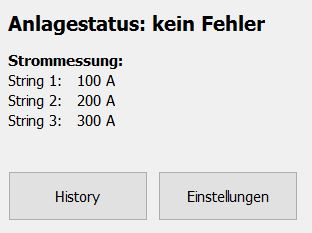
\includegraphics[width=0.45\textwidth]{images/userguide/screen0.png}
    \caption{Hauptmenu}
    \label{fig:userguide:screen0}
\end{wrapfigure}

Bei Bet\"atigung des gr\"unen Knopfes  erscheint das Hauptmenu, dargestellt in
Abbildung \ref{fig:userguide:screen0}. Dieses dient  einerseits zur Auflistung
aktueller  Messwerte der  Strangstr\"ome  und  des Anlagestatus,  andererseits
f\"uhrt  es mittels  weiterer  Buttons in  die  jeweiligen Untermenus. In  der
obersten Zeile  \emph{Anlagestatus} wird  dargestellt, ob  ein Problem  an der
Anlage vorliegt. Wird bei Anlagestatus  \emph{kein Fehler} angezeigt, liegt an
der  Anlage keine  St\"orung vor. Wird  jedoch die  Fehlfunktion eines  Moduls
detektiert, erfolgt eine Meldung im Hauptmenu. (Weiter Infos zum St\"orbetrieb
im Kapitel weiter unten).

\noindent\adjustbox{valign=t}{\begin{minipage}{0.475\textwidth}
    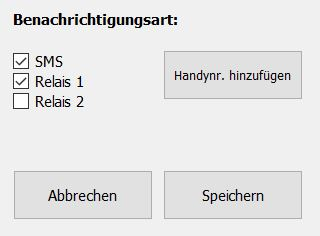
\includegraphics[width=\textwidth]{images/userguide/screen1.png}
    \figcaption[Master: Menu: Einstellungen]{Einstellungen}
    \label{fig:userguide:screen1}
\end{minipage}}
\noindent\adjustbox{valign=t}{\begin{minipage}{0.475\textwidth}
    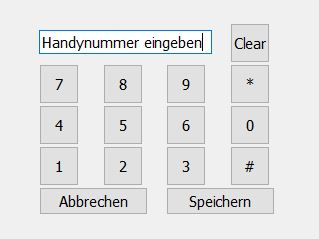
\includegraphics[width=\textwidth]{images/userguide/screen2.png}
    \figcaption[Master: Menu: Einstellungen: Telefonnummer]{Eingabe einer Telefonnummer}
    \label{fig:userguide:screen2}
\end{minipage}}

Im     Untermenu     \emph{Einstellungen},    dargestellt     in     Abbildung
\ref{fig:userguide:screen1},   k\"onnen  die   SMS-Benachrichtigung  und   die
Relaisausg\"ange konfiguriert werden. Beim  Hinzuf\"ugen einer Handynummer mit
korrekter Vorwahl  (Bsp. \code{0041 79  612 33  22}) und bei  Bet\"atigung des
entsprechenden K\"astchens   wird automatisch die Benachrichtigung  \"uber SMS
aktiviert. Das zugeh\"orige Menu  ist in Abbildung \ref{fig:userguide:screen2}
gezeigt. Wie auch die beiden Relais 1 und Relais 2 werden bei der Bet\"atigung
des jeweiligen K\"astchens aktiviert. \"Uber den Button \emph{Speichern} werden
die Einstellungen im System \"ubernommen.


% ---------------------------------------------------------------------------- %
\section{St\"orbetrieb}
\label{sec:userguide:errors}
% ---------------------------------------------------------------------------- %

Wird die Fehlfunktion eines  Moduls detektiert, erfolgt eine St\"orungsmeldung
an das  Master-Ger\"at. Folglich erscheint  im Hauptmenu  des Master-Ger\"ates
die  Seriennummer des  entsprechenden Moduls  wie auch  Datum und  Uhrzeit der
Fehlererkennung, wie in Abbildung \ref{fig:userguide:screen3} gezeigt.

Zeitgleich  werden  am  Master-Ger\"at  zwei  Relaiskontakte  bet\"atigt,  die
f\"ur externe  akustische oder  optische Meldeger\"ate  vorgesehen sind. Diese
externen Meldeger\"ate lassen sich mit  dem entsprechenden Button im Hauptmenu
quittieren. Sofern  unter  \emph{Einstellungen}  eine  Handynummer  hinterlegt
wurde, erfolgt  zus\"atzlich eine Fehlerbenachrichtigung an  das entsprechende
Mobiltelefon.

Um die Energieverluste zu minimieren, sollte bei einem Fehlerfall umgehend ein
Installateur der Photovoltaikanlage konsultiert werden. Sobald das fehlerhafte
Modul  wieder einwandfrei  funktioniert, wird  die Fehlermeldung  im Hauptmenu
des  Master-Ger\"ates  automatisch ausgeblendet. Im  Untermenu  \emph{History}
(Abbildung  \ref{fig:userguide:screen4} sind  alle bisherigen  Fehlermeldungen
der Anlage ersichtlich.

\noindent\adjustbox{valign=t}{\begin{minipage}{0.475\textwidth}
    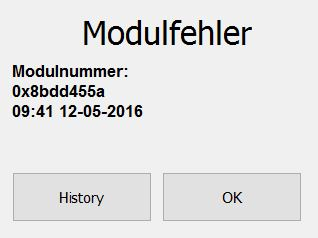
\includegraphics[width=\textwidth]{images/userguide/screen3.png}
    \figcaption[Master: Menu: Modulfehler]{Fehler bei einem Modul}
    \label{fig:userguide:screen3}
\end{minipage}}
\noindent\adjustbox{valign=t}{\begin{minipage}{0.475\textwidth}
    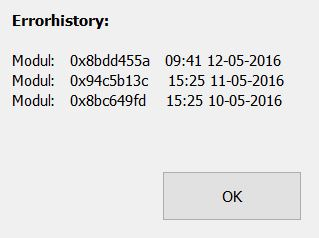
\includegraphics[width=\textwidth]{images/userguide/screen4.png}
    \figcaption[Master: Menu: Einstellungen: History]{Fehler-History der Anlage}
    \label{fig:userguide:screen4}
\end{minipage}}

Was  l\"auft? Was  l\"auft  nicht? Weshalb? Weiteres Vorgehen  bei  gen\"ugend
Zeit? Schwierigkeiten w\"ahren des Projekts?



% -------------------------------------------------------- %
% Appendices are  usually numbered  and therefore  part of %
% the mainmatter, not the backmatter.                      %
% The advice about meaningful chapter names applies to the %
% appendices as well, see above.                           %
% -------------------------------------------------------- %
\appendixpage
\appendix
%% **************************************************************************** %
\chapter{Parameter des Solarzellenmodells}
\label{app:celldata}
% **************************************************************************** %

Zur  Herleitung  der  Zellenparameter  werden vier  Quellen  herangezogen,  um
ein  einigermassen  gut  abgest\"utztes Ergebnis  zu  erhalten. Die  gesuchten
Parameter sollen  f\"ur am Markt  erh\"altliche Module g\"ultig  sein, weshalb
Datenbl\"atter von Solar\emph{modulen} und nicht Zellen verwendet werden.

Zuerst  werden  Zellenstrom  und Zellenspannung  bestimmt,  anschliessend  die
Fl\"ache einer Zelle,  um damit auf die im Modell  verwendete Kapazit\"at, den
Shunt-Widerstand und den Seriewiderstand schliessen zu k\"onnen.


% ---------------------------------------------------------------------------- %
\section{Zellenstrom und Zellenspannung}
\label{app:sec:cell:UI}
% ---------------------------------------------------------------------------- %

Tabelle   \ref{tab:moduleData:IU}    auf   Seite   \pageref{tab:moduleData:IU}
enth\"alt die  Daten zu  Kurzschlussstr\"omen und Leerlaufspannungen  von vier
Modulen. Die  Spannung  $U_{\mathrm{OC,  Zelle}}$ pro  Zelle  (letzte  Spalte)
errechnet sich gem\"ass:

\begin{equation}
    \label{eq:voltagePerCell}
    U_{\mathrm{OC, Zelle}} = \frac{U_{\mathrm{OC, Strang}}}{\text{Anzahl Zellen pro Strang}}
\end{equation}

\begin{table}
    \centering
    \small
    \caption{%
        Daten   f\"ur   Solarmodule.  \textbf{pk}:   polykristallines   Panel,
        \textbf{mk}:     monokristallines     Panel.     \emph{Anmerkung}: Die
        Konfiguration  der Module  (wieviele  Zellen in  Serie  und wie  viele
        Str\"ange  parallel)  ist  mit   Ausnahme  des  Solarex  MSX-60  nicht
        angegeben. Es  ist  aber  bekannt,  in  welcher  Gr\"ossenordnung  die
        Spannung  pro  Zelle  ungef\"ahr  liegen sollte,  womit  man  aus  den
        angegebenen  Leerlaufspannungen  und  der Gesamtzahl  Zellen  auf  die
        Konfiguration eines Modules schliessen kann.%
    }
    \label{tab:moduleData:IU}
    \begin{tabular}{lp{20mm}lllll}
        \toprule
          \rotatebox{70}{\pbox{25mm}{Quelle}}
        & \rotatebox{70}{\pbox{25mm}{Modell}}
        & \rotatebox{70}{\pbox{25mm}{Kurzschluss-\\strom $I_{\mathrm{SC}}$}}
        & \rotatebox{70}{\pbox{25mm}{Leerlauf-\\spannung $V_{\mathrm{OC}}$}}
        & \rotatebox{70}{\pbox{25mm}{Anzahl Zellen \\(total)}}
        & \rotatebox{70}{\pbox{25mm}{Anzahl Zellen \\(Strang)}}
        & \rotatebox{70}{\pbox{25mm}{Leerlaufspan-\\nung pro Zelle}} \\
        \midrule

          \cite{ref:solar:bonkoungou}
        & Solarex MSX-60
        & \SI{3.8}{\ampere}
        & \SI{21.1}{\volt}
        & \num{36}
        & \num{36}
        & \SI{586}{\milli\volt}
        \\

          \cite{ref:solar:px85}
        & Sunset PX85 (\textbf{pk})
        & \SI{5.5}{\ampere}
        & \SI{21.5}{\volt}
        & \num{76}
        & \num{38}
        & \SI{566}{\milli\volt}
        \\

          \cite{ref:solar:as150}
        & Sunset Solargenerator AS150 (\textbf{mk})
        & \SI{8.7}{\ampere}
        & \SI{22.3}{\volt}
        & \num{36}
        & \num{36}
        & \SI{620}{\milli\volt}
        \\

          \cite{ref:solar:sunmodulePro}
        & Sunmodule Pro-Series XL SW320 (\textbf{mk})
        & \SI{9.41}{\ampere}
        & \SI{45.9}{\volt}
        & \num{72}
        & \num{72}
        & \SI{638}{\milli\volt}
        \\

        \bottomrule
    \end{tabular}
\end{table}

Wir verwenden f\"ur  die Simulation einer Zelle den  gerundeten Mittelwert der
Zellenspannungen aus der letzten Spalte von Tabelle \ref{tab:moduleData:IU}:

\begin{equation}
    \label{eq:cell:UOC}
    \underline{\underline{U_{\mathrm{OC, Zelle, Simu}} = \SI{600}{\milli\volt}}}
\end{equation}

Polykristalline  Zellen  liefern  bedeutend  kleinere  Kurzschlusstr\"ome  als
monokristalline  Zellen.  Jedoch  werden bei  monokristallinen Zellen  weniger
Str\"ange parallel  geschaltet, womit  der Gesamtstrom  des Moduls  immer noch
unter \SI{10}{\ampere}  bleibt. Unabh\"angig vom  genauen Aufbau  eines Moduls
gehen wir  daher davon aus,  dass es  nicht mehr als  \SI{10}{\ampere} liefern
wird.


% ---------------------------------------------------------------------------- %
\section{Bestimmung der Zellenfl\"ache}
\label{app:sec:cell:surface}
% ---------------------------------------------------------------------------- %

Das    PX-85-Modul   aus    \cite{ref:solar:px85}    verwendet   76    Zellen,
angeordnet  in   einer  $4  \times  19$   -  Konfiguration. Seine  Abmessungen
betragen   $\SI{1477}{\milli\meter}    \times   \SI{660}{\milli\meter}$,   was
sich   herunterrechnen  l\"asst   auf  eine   ungef\"ahre  Modulgr\"osse   von
$\SI{165}{\milli\meter}   \times   \SI{75}{\milli\meter}$. Dabei  werden   die
Abmessungen   des   Rahmens   und   die  Abst\"ande   zwischen   den   Modulen
vernachl\"assigt.

Die Fl\"ache  des AS-150-Moduls wird analog  aus Quelle~\cite{ref:solar:as150}
zu  $\SI{155}{\milli\meter}  \times   \SI{164}{\milli\meter}$  bestimmt.   Das
XL-320-Modul   aus   \cite{ref:solar:sunmodulePro}    hat   die   Zellgr\"osse
direkt    angegeben,    sie     betr\"agt    $\SI{156}{\milli\meter}    \times
\SI{156}{\milli\meter}$. Es ist naheliegend dass aufgrund von Standardisierung
das AS-150-Modul die gleiche Zelldimension hat wie das XL-320-Modul, n\"amlich
den verbreiteten 6-Zoll-Formfaktor.

Da  eine gr\"ossere  Zelle eine  gr\"ossere Kapazit\"at  und somit  gr\"ossere
Probleme   im  Falle   der  Kurzschlussvariante   bedeutet,  wird   mit  einer
Zellgr\"osse   von   $\SI{156}{\milli\meter}  \times   \SI{156}{\milli\meter}$
gerechnet, womit sich die Fl\"ache der Zelle bestimmt zu:

\begin{equation}
    \label{eq:cell:surface}
    \underline{\underline{A_{\mathrm{Zelle}} = \SI{156}{\milli\meter} \times \SI{156}{\milli\meter} = \SI{243.36}{\centi\meter\squared}}}
\end{equation}

Dies     entspricht     ungef\"ahr     der     600-fachen     Fl\"ache     des
\SI{0.43}{\centi\meter\squared}-Modules aus  Quelle \cite{ref:solar:scofield}.

%% ---------------------------------------------------------------------------- %
\chapter{Vereinfachtes Modell f\"ur ein PV-Modul}
\label{app:models:develop:module:simple}
% ---------------------------------------------------------------------------- %

Zur  Reduktion des  Rechenaufwands im  Vergleich zu  dem im  vorigen Abschnitt
entwickelten Modell soll ein vereinfachtes Modell eines Solarmoduls entwickelt
werden.

Ausgangspunkt   ist   das   Eindiodenmodell    einer   Zelle   aus   Abbildung
\todo{reference}, f\"ur  welches die Parameter  so angepasst werden,  dass das
Verhalten des aus Zellen aufgebauten Modells aus dem vorigen Abschnitt und des
vereinfachten Modells zufriedenstellend \"ubereinstimmen.

Das Vorgehen ist dabei wie folgt: \todo{Eigentliche Werte}

\begin{itemize}
    \item
        Die parasit\"are  Kapazit\"at des  Moduls wird angepasst  gem\"ass dem
        Gesetz zur Serieschaltung von Kapazit\"aten:
        $C_{\mathrm{p, Modul}} = C_{\mathrm{p, Zelle}} \div \text{Anzahl Zellen}$
    \item
        Der Seriewiderstand des Moduls ist die Summe der Seriewiderst\"ande aller
        Zellen
    \item
        Der  Parallele   Widerstand  wird   entsprechend  der   Anzahl  Zellen
        hochgerechnet.
        \todo{kein Einfluss, verifikation}
    \item
        Der Reverse  Saturation Current  des Moduls ist  von der  Fl\"ache des
        Moduls abh\"angig und  wird als Startwert vorerst  gem\"ass der Anzahl
        Module hochgerechnet.
    \item
        Der  Idealit\"atsfaktor ist  ein Indikator  f\"ur den  Spannungsabfall
        \"uber   einer   Diode   bei   einem   bestimmten   Strom   \todo{ref:
        abbildung}. Bei  einer Serieschaltung  von Dioden  sollte entsprechend
        mehr   Spannung    \"uber   dem   gesamten   Strang    abfallen   (bei
        gleichbleibendem  Strom). Der Startwert  f\"ur den  Idealit\"atsfaktor
        des vereinfachten Modells wird  deshalb entsprechend der Anzahl Zellen
        im Modul skaliert.
\end{itemize}

Gem\"ass dieser Methodik werden die Startwerte festgelegt auf:

\begin{itemize}
    \firmlist
    \item
        $C_{\mathrm{p, Modul}} = \SI{167}{\nano\farad}$
    \item
        $R_{\mathrm{S}} = \SI{12}{\milli\ohm}$
    \item
        $R_{\mathrm{Shunt}} = \SI{60}{\kilo\ohm}$
    \item
        $I_{\mathrm{S}} = \SI{288}{\milli\ampere}$
    \item
        $n = 118$
\end{itemize}

Mit diesen  Werten werden verschiedene  Szenarien simuliert und  die Resultate
mit den  Ergebnissen des komplexeren Modells  verglichen. Durch Iteration wird
$I_{\mathrm{S}}$ schlussendlich  auf \SI{2.88}{\micro\ampere}  festgelegt, was
kurioserweise kleiner ist als der Wert einer einzelnen Diode.

Abbildungen
\ref{fig:model:simpel:verif:current:mosfet:freq},
\ref{fig:model:simpel:verif:voltage:mosfet:freq},
\ref{fig:model:simpel:verif:current:RL:freq} und
\ref{fig:model:simpel:verif:current:mosfet:time} stellen die Resultate
verschiedener Simulationen mit und ohne Last f\"ur das vereinfachte Modell und
das zellenbasierte  Modell graphisch dar.   Wie zu erkennen ist,  besteht eine
gute \"Ubereinstimmung.

%Parasit\"are Kapazit\"at: Kapazit\"at einer Zelle / anzahl Zellen \\
%Serie widerstand: widerstand einzelzelle * anzahl zellen \\
%shunt widerstand: widerstand einer zelle / anzahl zellen \\
%IS: IS einzelzelle * anzahl zellen (0.288m) -> anpassen, bis frequenzgang und zeitplot passend \\
%N: N einzelzelle * anzahl zellen \\
%Shockley diode model \\
\todo{Einheiten achsen, auflistung parameter, schaltkreise zu plots, LTspice diagramme}


\begin{figure}
    \begin{tikzpicture}
       \begin{scope}[x={(0mm,0mm)},y={(90mm,0.9\textwidth)}]
           \begin{axis}[%
                   xmode=log,
                   height=45mm,
                   width=0.9\textwidth,
                   at={(0,45mm)},
                   grid=both,
                   xlabel=Frequenz (\si{\hertz}),
                   ylabel=Strom (\si{\deci\bel}),
               ]
                \addplot[color=blue] table {data/simple-model-verification/module-72cells-series--reference--freq-sweep-over-mosfet-no-load--I--magn.dat};
                \addplot[color=magenta] table {data/simple-model-verification/module-simple-72x1--freq-sqeep-over-mosfet-no-load--I--magn.dat};
           \end{axis}
           \begin{axis}[%
                   xmode=log,
                   height=45mm,
                   width=0.9\textwidth,
                   at={(0,0)},
                   grid=both,
                   xlabel=Frequenz (\si{\hertz}),
                   ylabel=Phase (\si{\degree}),
               ]
                \addplot[color=blue] table {data/simple-model-verification/module-72cells-series--reference--freq-sweep-over-mosfet-no-load--I--phase.dat};
                \addplot[color=magenta] table {data/simple-model-verification/module-simple-72x1--freq-sqeep-over-mosfet-no-load--I--phase.dat};
           \end{axis}
       \end{scope}
   \end{tikzpicture}
    \caption{Frequenzgang des Stroms durch den MOSFET bei einer Beschaltung ohne zus\"atzliche Last}
    \label{fig:model:simpel:verif:current:mosfet:freq}
\end{figure}

\begin{figure}
    \begin{tikzpicture}
       \begin{scope}[x={(0mm,0mm)},y={(90mm,0.9\textwidth)}]
           \begin{axis}[%
                   xmode=log,
                   height=45mm,
                   width=0.9\textwidth,
                   at={(0,45mm)},
                   grid=both,
                   xlabel=Frequenz (\si{\hertz}),
                   ylabel=Spannung (\si{\deci\bel}),
               ]
                \addplot[color=blue] table {data/simple-model-verification/module-72cells-series--reference--freq-sweep-over-mosfet-no-load--U--magn.dat};
                \addplot[color=magenta] table {data/simple-model-verification/module-simple-72x1--freq-sweep-over-mosfet-no-load--U--magn.dat};
           \end{axis}
           \begin{axis}[%
                   xmode=log,
                   height=45mm,
                   width=0.9\textwidth,
                   at={(0,0)},
                   grid=both,
                   xlabel=Frequenz (\si{\hertz}),
                   ylabel=Phase (\si{\degree}),
               ]
                \addplot[color=blue] table {data/simple-model-verification/module-72cells-series--reference--freq-sweep-over-mosfet-no-load--U--phase.dat};
                \addplot[color=magenta] table {data/simple-model-verification/module-simple-72x1--freq-sweep-over-mosfet-no-load--U--phase.dat};
           \end{axis}
       \end{scope}
   \end{tikzpicture}
    \caption{Frequenzgang der Spannung \"uber dem MOSFET bei einer Beschaltung ohne zus\"atzliche Last}
    \label{fig:model:simpel:verif:voltage:mosfet:freq}
\end{figure}

\begin{figure}
    \begin{tikzpicture}
       \begin{scope}[x={(0mm,0mm)},y={(90mm,0.9\textwidth)}]
           \begin{axis}[%
                   xmode=log,
                   height=45mm,
                   width=0.9\textwidth,
                   at={(0,45mm)},
                   grid=both,
                   xlabel=Frequenz (\si{\hertz}),
                   ylabel=Spannung (\si{\deci\bel}),
               ]
                \addplot[color=blue] table {data/simple-model-verification/module-72cells-series--reference--freq-sweep-over-Rload--100ohm-100uF--I--magn.dat};
                \addplot[color=magenta] table {data/simple-model-verification/module-simple-72x1--freq-sweep-over-Rload--100ohm-100uF--I--magn.dat};
           \end{axis}
           \begin{axis}[%
                   xmode=log,
                   height=45mm,
                   width=0.9\textwidth,
                   at={(0,0)},
                   grid=both,
                   xlabel=Frequenz (\si{\hertz}),
                   ylabel=Phase (\si{\degree}),
               ]
                \addplot[color=blue] table {data/simple-model-verification/module-72cells-series--reference--freq-sweep-over-Rload--100ohm-100uF--I--phase.dat};
                \addplot[color=magenta] table {data/simple-model-verification/module-simple-72x1--freq-sweep-over-Rload--100ohm-100uF--I--phase.dat};
           \end{axis}
       \end{scope}
   \end{tikzpicture}
   \caption{Frequenzgang des Stroms durch den Lastwiderstand bei einer Last von \SI{100}{\ohm} parallel zu \SI{100}{\micro\farad}}
    \label{fig:model:simpel:verif:current:RL:freq}
   %\label{fig:freqresponse:module:simple}
\end{figure}


\begin{figure}
    \begin{tikzpicture}
       \begin{scope}[x={(0mm,0mm)},y={(60mm,0.9\textwidth)}]
           \begin{axis}[%
                   height=60mm,
                   width=0.9\textwidth,
                   at={(0,0)},
                   grid=both,
                   xlabel=Zeit (\si{\second}),
                   ylabel=Strom (\si{\ampere}),
               ]
                \addplot[color=blue] table {data/simple-model-verification/module-72cells-series--reference--time-domain-over-mosfet-10kHz--I.dat};
                \addplot[color=magenta] table {data/simple-model-verification/module-simple-72x1--time-domain-over-mosfet--10kHz--I.dat};
           \end{axis}
       \end{scope}
   \end{tikzpicture}
    \caption{Zeitlicher Verlauf des Stroms durch den MOSFET bei einer Beschaltung ohne zus\"atzliche Last}
    \label{fig:model:simpel:verif:current:mosfet:time}
\end{figure}

% **************************************************************************** %
\chapter{Daten von Solarmodulen}
\label{app:commercial:modules}
% **************************************************************************** %

Dieser Abschnitt enth\"alt in  Tabelle \ref{tab:moduleData:IU} einige Eckdaten
von kommerziell  erh\"altlichen Modulen  mit den  zugeh\"origen Quellen. Diese
Informationen sollen  prim\"ar als Anhaltspunkt und  Vergleich zwischen Praxis
und unseren Simuationen dienen.

\begin{table}
    \centering
    \small
    \caption{%
        Daten   f\"ur   Solarmodule.  \textbf{pk}:   polykristallines   Panel,
        \textbf{mk}:     monokristallines     Panel.     \emph{Anmerkung}: Die
        Konfiguration  der Module  (wieviele  Zellen in  Serie  und wie  viele
        Str\"ange  parallel)  ist  mit   Ausnahme  des  Solarex  MSX-60  nicht
        angegeben. Es  ist  aber  bekannt,  in  welcher  Gr\"ossenordnung  die
        Spannung  pro  Zelle  ungef\"ahr  liegen sollte,  womit  man  aus  den
        angegebenen Leerlaufspannungen  und der Gesamtzahl der  Zellen auf die
        Konfiguration eines Modules schliessen kann.%
    }
    \label{tab:moduleData:IU}
    \begin{tabular}{lp{20mm}lllll}
        \toprule
          \rotatebox{70}{\pbox{25mm}{Quelle}}
        & \rotatebox{70}{\pbox{25mm}{Modell}}
        & \rotatebox{70}{\pbox{25mm}{Kurzschluss-\\strom $I_{\mathrm{SC}}$}}
        & \rotatebox{70}{\pbox{25mm}{Leerlauf-\\spannung $V_{\mathrm{OC}}$}}
        & \rotatebox{70}{\pbox{25mm}{Anzahl Zellen \\(total)}}
        & \rotatebox{70}{\pbox{25mm}{Anzahl Zellen \\(Strang)}}
        & \rotatebox{70}{\pbox{25mm}{Leerlaufspan-\\nung pro Zelle}} \\
        \midrule

          \cite{ref:solar:bonkoungou}
        & Solarex MSX-60
        & \SI{3.8}{\ampere}
        & \SI{21.1}{\volt}
        & \num{36}
        & \num{36}
        & \SI{586}{\milli\volt}
        \\

          \cite{ref:solar:px85}
        & Sunset PX85 (\textbf{pk})
        & \SI{5.5}{\ampere}
        & \SI{21.5}{\volt}
        & \num{76}
        & \num{38}
        & \SI{566}{\milli\volt}
        \\

          \cite{ref:solar:as150}
        & Sunset Solargenerator AS150 (\textbf{mk})
        & \SI{8.7}{\ampere}
        & \SI{22.3}{\volt}
        & \num{36}
        & \num{36}
        & \SI{620}{\milli\volt}
        \\

          \cite{ref:solar:sunmodulePro}
        & Sunmodule Pro-Series XL SW320 (\textbf{mk})
        & \SI{9.41}{\ampere}
        & \SI{45.9}{\volt}
        & \num{72}
        & \num{72}
        & \SI{638}{\milli\volt}
        \\

        \bottomrule
    \end{tabular}
\end{table}


%\begin{table}[h!tb]
%    \centering
%    \caption{Abmessungen der Solarmodule aus Tabelle \ref{tab:moduleData:IU}}
%    \label{tab:moduleData:Dimensions}
%    \begin{tabular}{lp{20mm}ll}
%        \toprule
%          \rotatebox{70}{\pbox{25mm}{Quelle}}
%        & \rotatebox{70}{\pbox{25mm}{Modell}}
%        & \rotatebox{70}{\pbox{25mm}{Abmessungen Modul ($\si{\milli\meter} \si{\milli\meter}$)}}
%        & \rotatebox{70}{\pbox{25mm}{Abmessungen Zelle ($\si{\milli\meter} \si{\milli\meter}$)}} \\
%        \midrule
%
%          \cite{ref:solar:px85}
%        & Sunset PX85 (\textbf{pk})
%        & $1477 \times 660$
%        & $\approx 165 \times 75$
%        \\
%
%          \cite{ref:solar:as150}
%        & Sunset Solargenerator AS150 (\textbf{mk})
%        & $1480 \times 660$
%        & $\approx 155 \times 164$
%        \\
%
%          \cite{ref:solar:sunmodulePro}
%        & Sunmodule Pro-Series XL SW320 (\textbf{mk})
%        & $1985 \times 990$
%        & $156 \times 156$
%        \\
%        \bottomrule
%    \end{tabular}
%\end{table}

% **************************************************************************** %
\chapter{\code{LTspice}-Schaltungen}
\label{app:ltspice}
% **************************************************************************** %

Dieses Kapitel  beinhaltet \code{LTspice}-Schaltungen, welche  zu Simulationen
benutzt worden sind. Erkl\"arungen  zu den jeweiligen Schaltungen  sind in den
Kapiteln  zu finden,  welche auf  sie verweisen. S\"amtliche  Schaltungen sind
auch elektronisch als \code{.asc}-Datei verf\"ugbar.

\noindent\begin{minipage}{\textwidth}
    \centering
    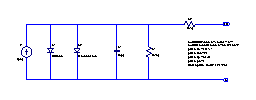
\includegraphics[width=0.9\textwidth]{images/ltspice/generic-iv-curves/cell.eps}
    \figcaption[\code{LTspice}-Schaltung f\"ur PV-Zelle]{%
        Modell   der   PV-Zelle,   aus   welchem  das   Modul   in   Abbildung
        \label{fig:ltspice:iv:generic:module} aufgebaut  ist. Die Simulationen
        aus   Abbildung   \ref{fig:simu:iv-curves:module:generic}  auf   Seite
        \pageref{fig:simu:iv-curves:module:generic}   basieren    auf   diesem
        Modell. Gegen\"uber     in     Abschnitt     \ref{sec:simu:model:cell}
        hergeleiteten Modell hat dieses  Modell einen h\"oheren Photostrom und
        einen niedrigeren Shunt-Widerstand. Dies  erzeugt etwas anschaulichere
        Kurven.%
    }
    \label{fig:ltspice:iv:generic:cell}
    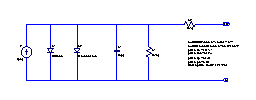
\includegraphics[width=0.9\textwidth]{images/ltspice/jac/cell.eps}
    \figcaption[\code{LTspice}-Schaltung f\"ur PV-Zelle]{%
        Modell  der   PV-Zelle,  auf  welchen  die   Simulationen  in  Kapitel
        \ref{chap:simu} ab  Seite \pageref{chap:simu}  beruhen. Die Herleitung
        ist in Abschnitt \ref{sec:simu:model:cell} dokumentiert.%
    }
    \label{fig:ltspice:jac:cell}
\end{minipage}

\begin{figure}[h!tb]
    \centering
    \begin{tikzpicture}[%
        spy scope = {magnification=7,size=25*8,connect spies},
        every spy on node/.style={circle,red,draw},
        every spy in node/.style = {circle, fill=white, fill opacity=1, draw},
        ]
        \node[inner sep = 0pt,anchor=south west] {%
            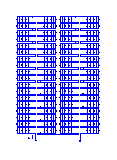
\includegraphics[width=\textwidth]{images/ltspice/generic-iv-curves/module.eps}
        };
        \spy[red] on (0.45,1.2) in node at (10,8);
    \end{tikzpicture}
    \caption[\code{LTspice}-Schaltung f\"ur PV-Modul f\"ur IV- und PV-Kurven]{%
        \code{LTspice}-Modell,    welches    zur    Erzeugung    der    Kurven
        in   Abbildung   \ref{fig:simu:iv-curves:module:generic}   auf   Seite
        \pageref{fig:simu:iv-curves:module:generic}  benutzt  worden  ist. Das
        Modell  der Zelle,  aus welcher  dieses  Modul aufgebaut  ist, ist  in
        Abbildung \ref{fig:ltspice:iv:generic:cell} abgebildet.%
    }
    \label{fig:ltspice:iv:generic:module}
\end{figure}

\begin{figure}[h!tb]
    \centering
    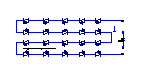
\includegraphics[width=\textwidth]{images/ltspice/jac/stringNoD.eps}
    \caption[\code{LTspice}-Schaltung f\"ur Modulstrang]{%
        \code{LTspice}-Schaltung  f\"ur  einen   Modulstrang  aus  20  Modulen
        und   variablem  Lastwiderstand   \code{Rload}   zur  Erstellung   von
        Strom-Spannungs-Kurven. Es  wird   je  ein  Strang  aus   Modulen  mit
        Freilaufdiode   (Abbildung  \ref{fig:ltspice:jacModule:NoDiode})   und
        ohne   Freilaufdiode   (Abbildung   \ref{fig:ltspice:jacModule:Diode})
        simuliert.%
    }
    \label{fig:ltspice:string:ivCurve}
\end{figure}

\begin{figure}[h!tb]
    \centering
    \begin{tikzpicture}[%
        spy scope = {magnification=5,height=25*5.5,width=25*10,connect spies},
        every spy on node/.style={rectangle,red,draw},
        every spy in node/.style = {rectangle,fill=white, fill opacity=1, draw},
        ]
        \node[inner sep = 0pt,anchor=south west] {%
            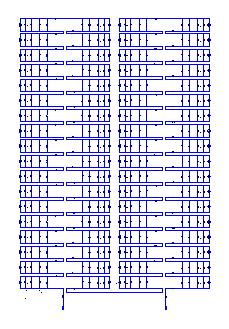
\includegraphics[width=\textwidth]{images/ltspice/jac/jacModuleNoD.eps}
        };
        \spy[red] on (1.15,1.13) in node at (9,8);
    \end{tikzpicture}
    \caption[\code{LTspice}-Schaltung f\"ur PV-Modul ohne Freilaufdiode]{%
        Modul    ohne   Freilaufdiode,    benutzt    f\"ur   die    Simulation
        aus   Abbildung   \ref{fig:simu:iv-curves:array:generic}   von   Seite
        \pageref{fig:simu:iv-curves:array:generic}.%
    }
    \label{fig:ltspice:jacModule:NoDiode}
\end{figure}

\begin{figure}[h!tb]
    \centering
    \begin{tikzpicture}[%
        spy scope = {magnification=5,height=25*5.5,width=25*10,connect spies},
        every spy on node/.style={red,draw},
        every spy in node/.style = {fill=white, fill opacity=1, draw},
        ]
        \node[inner sep = 0pt,anchor=south west] {%
            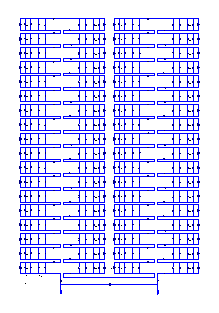
\includegraphics[width=\textwidth]{images/ltspice/jac/jacModule.eps}
        };
        \spy[rectangle,red] on (1.15,1.13) in node at (9,8);
        \spy[circle,size=25*3,red] on (7.05,0.9) in node at (9,3);
    \end{tikzpicture}
    \caption[\code{LTspice}-Schaltung f\"ur PV-Modul mit Freilaufdiode]{%
        Modul      mit      Freilaufdiode       (unten,      Mitte,      Diode
        \code{D145}). Benutzt       f\"ur       die       Simulation       aus
        Abbildung   \ref{fig:simu:iv-curves:array:generic:bypass}  von   Seite
        \pageref{fig:simu:iv-curves:array:generic:bypass}       sowie      die
        Simulationen zu den L\"osungsvarianten in Abschnitt
        \ref{sec:simu:coupling:inductive} ab Seite
        \pageref{sec:simu:coupling:inductive}, Abschnitt
        \ref{sec:simu:coupling:capacitive} ab Seite
        \pageref{sec:simu:coupling:capacitive} und Abschnitt
        \ref{sec:simu:short} ab Seite
        \pageref{sec:simu:short}.
        Abbildung   \ref{fig:ltspice:jac:cell}    enth\"alt   das   verwendete
        Zellenmodell.%
    }
    \label{fig:ltspice:jacModule:Diode}
\end{figure}

% **************************************************************************** %
\chapter{Schemata}
\label{app:chap:schemas}
% **************************************************************************** %
{\begin{a3pages}

\begin{tikzpicture}[remember picture,overlay]
    \node[inner sep=0pt] at (current page.center) {%
        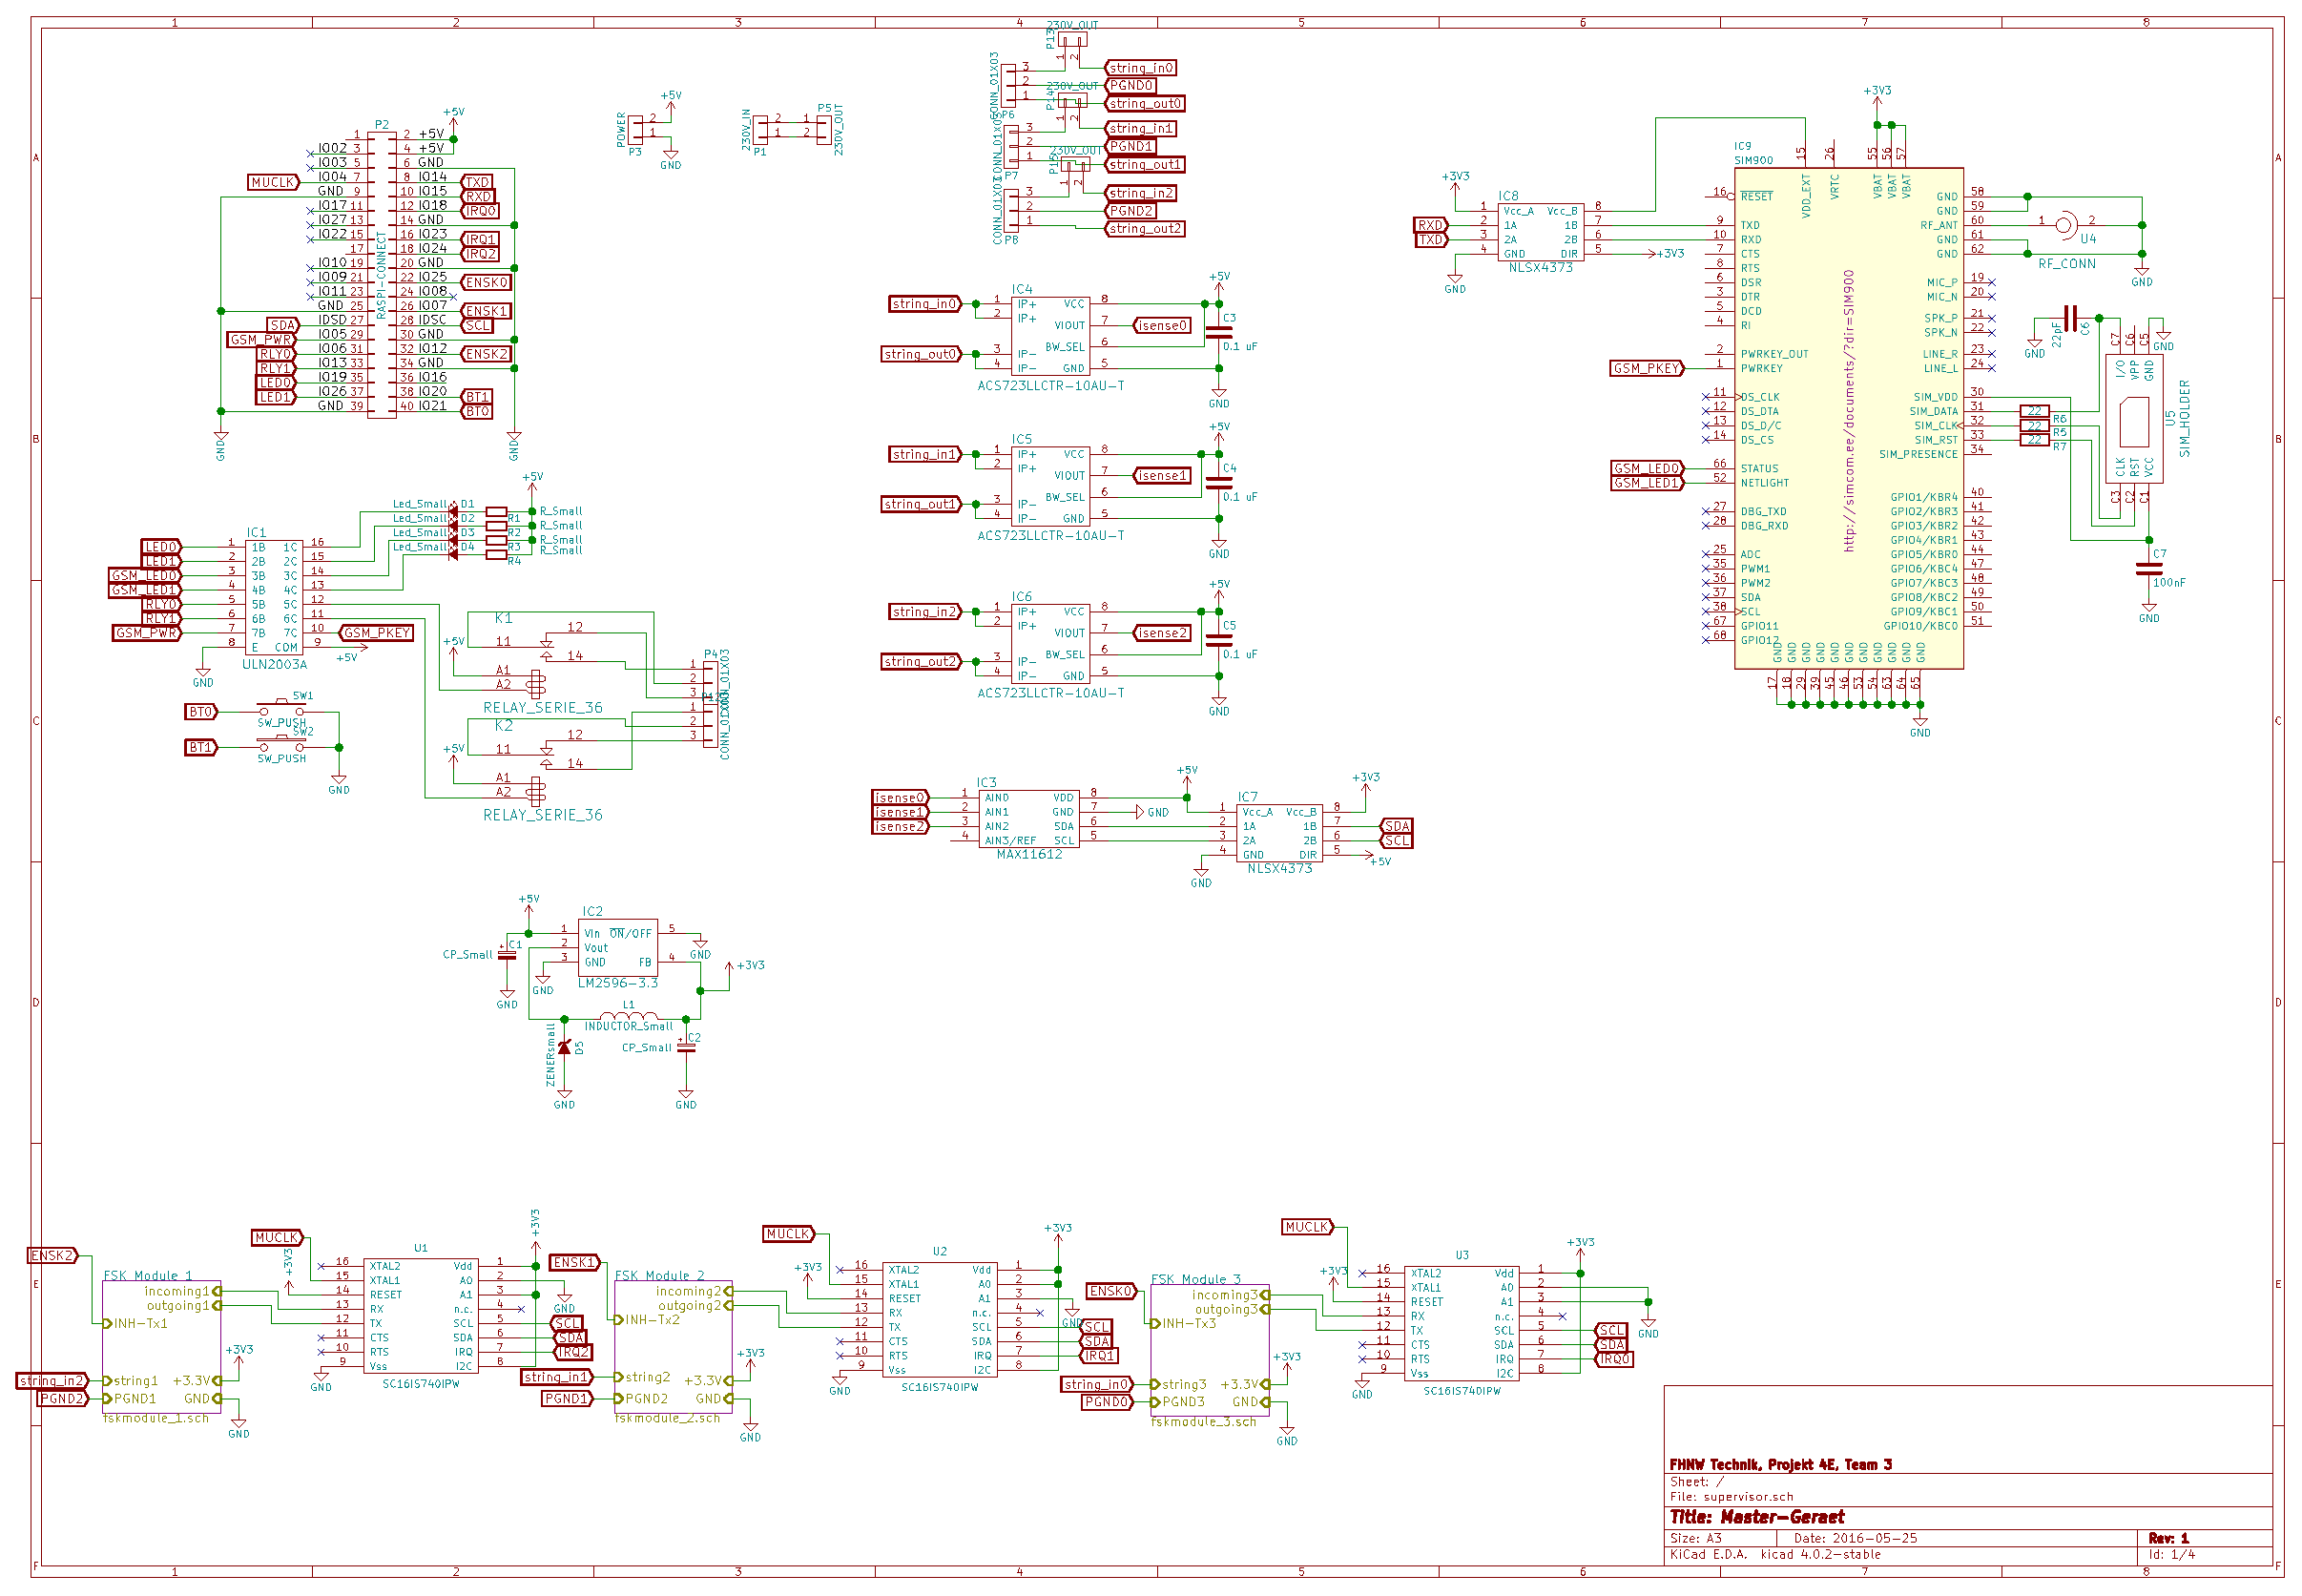
\includegraphics{images/superv-sch/supervisor--sch.eps}%
    };
\end{tikzpicture}

\end{a3pages}}

%% **************************************************************************** %
\chapter{Modellierung eines Photovoltaik-Systems}
\label{chap:models}
% **************************************************************************** %

Bevor  simuliert  werden  kann,  m\"ussen  die  daf\"ur  ben\"otigten  Modelle
vorhanden  sein. In diesem  Abschnitt wird  im \emph{bottom-up}-Verfahren  das
Modell eines Strangs  aus PV-Modulen mit Zuleitung  entwickelt. Es wird zuerst
das Modell einer Zelle definiert, aus dem anschliessend ein PV-Modul aufgebaut
wird.  Das Modell  des PV-Moduls wird dann wiederum benutzt,  einen Strang aus
Modulen zu modellieren.

Die    entwickelten     Modelle    werden    anschliessend     im    Abschnitt
\emph{\titleref{chap:simu}} in \code{LTspice}-Simulationen verwendet, um unsere
L\"osungsans\"atze zu untersuchen.

\emph{Konvention:} Doppelt unterstrichene Werte in Gleichungen sind Parameter,
welche in unser Model aufgenommen werden.

% ---------------------------------------------------------------------------- %
\section{Modellierung einer PV-Zelle}
\label{sec:simu:model:cell}
% ---------------------------------------------------------------------------- %

\begin{wrapfigure}{r}{65mm}
    \centering
    % Simple Single-Diode Model
\begin{circuitikz}
    \footnotesize
    \draw
    % Source to top terminal
    (0,0) to[current source,i=$I_{\mathrm{Ph}}$] (0,2) -- (2,2) to[R,l^=$R_{\mathrm{S}}$] (4,2) node[ocirc] {}

    % Open terminal at bottom
    (4,0) node[ocirc] {} -- (0,0)

    % Voltage arrow over open terminals
    (4,1.7) -- (4,0.3) node[currarrow,rotate=-90] {}
    (4,1) node[anchor=west] {$V_{\mathrm{offen}}$}

    % Parallel elements
    (1,0) to[empty diode,*-*,l_=$D$] (1,2)
    (2,0) to[R,*-*,l_=$R_{\mathrm{Sh}}$] (2,2)
    ;
\end{circuitikz}

    \caption[Eindiodenmodell PV-Zelle]{%
        Eindiodenmodell  einer  PV-Zelle  mit  Stromquelle  $I_{\mathrm{Ph}}$,
        Diode  $D$,  Shunt-Widerstand $R_{\mathrm{Sh}}$~  und  Seriewiderstand
        $R_{\mathrm{S}}$.%
    }
    \label{fig:pvcell:1diode}
\end{wrapfigure}

Das Modell  einer idealien  Photovoltaikzelle ist  eine Stromquelle  mit einer
parallel geschalteten Diode. Da PV-Zellen in Realit\"at nicht ideal sind, wird
das einfachste Ersatzschaltbild einer PV-Zelle \"ublicherweise durch einen zur
Stromquelle parallel geschalteten Shunt-Widerstand $R_{\mathrm{Sh}}$ und einen
Seriewiderstand $R_{\mathrm{S}}$ erg\"anzt; das resultierende Ersatzschaltbild
ist in Abbildung \ref{fig:pvcell:1diode} dargestellt.

Die Genauigkeit  dieses Eindiodenmodells  ist jedoch h\"aufig  nicht besonders
gut  \cite{pvcell:phang}  \cite{pvcell:masmoudi}   (besonders  bei  niederigen
Beleuchtungsgraden),   weshalb   wir   hier  ein   Zweidiodenmodell   benutzen
werden. Eine  der  beiden  Dioden   modelliert  dabei  den  S\"attigungsstrom,
welcher von  Diffusionsprozessen verursacht wird, die  zweite Diode modelliert
den  S\"attigungsstrom,  welcher  von Rekombinationseffekten  verursacht  wird
\cite{pvcell:masmoudi}.

Zur Herleitung der Modellparamater existieren verschiedene Verfahren. Man kann
beispielsweise eine  PV-Zelle im Labor  ausmessen und die  Modellparameter aus
diesen  Messergebnissen  ableiten.   Dies  ist jedoch  nicht  immer  praktisch
realisierbar, da man allenfalls kein Testexemplar zur Verf\"ugung hat.  Sollen
bei  der  Messung  noch Fertigungstoleranzen  der  PV-Zellen  ber\"ucksichtigt
werden,  steigt der  experimentelle  (und  finanzielle) Aufwand  zus\"atzlich,
da  man  mehrere Exemplare  kaufen  und  ausmessen muss. Auch  die  Auswertung
erfordert mehr Arbeit, wenn  man mittels statistischer Methoden verl\"assliche
Schlussfolgerungen ziehen k\"onnen will.

Alternativ   kann   man   auch   versuchen,  die   Modellparameter   aus   dem
Datenblatt  einer  PV-Zelle  herzuleiten. Dies  bietet  zwei  haupts\"achliche
Vorteile: Einerseits  entfallen  aufw\"andige  Messungen   und  der  Kauf  von
Testexemplaren, andererseits ist davon auszugehen, dass der Hersteller mehrere
Exemplare ausgemessen hat  und typische Angaben in  den Datenbl\"atten gemacht
werden.  Es setzt jedoch voraus,  dass man den Herstellerangaben einigermassen
vertraut;  Sicherheit  ist  letztendlich  nur  durch  eigene  Verifikation  zu
erlangen.

Das Herleiten der Modellparameter aus den Herstellerangaben ist nicht trivial;
es wird deshalb  an dieser Stelle ein Modell  einer kommerziell erh\"altlichen
PV-Zelle  (M5SF-2 von  \emph{JA Solar})  als Grundlage  verwendet, welches  in
\cite{pvcell:masmoudi} hergeleitet und verifiziert worden ist.

\"Ublicherweise wird  bei PV-Zellen  nur das  Gleichstromverhalten untersucht;
das Verhalten  unter Wechselstrom interessiert meistens  nicht. Da das Signal,
welches  in  diesem  Projekt  auf die  DC-Leitung  aufmoduliert  wird,  jedoch
Wechselstrom  ist, muss  das  Wechselstromverhalten von  PV-Zellen in  unseren
Simulationen ber\"ucksichtigt werden.

Das  Zweidiodenmodell  aus  \cite{pvcell:masmoudi}  wird  deshalb  in  unseren
Simulationen noch durch eine parallele Kapazit\"at erg\"anzt, wie in Abbildung
\ref{fig:circuit:solarCell} gezeigt.

\begin{figure}[h!tb]
    \centering
    % Parametrized version, can be put at coordinates x and y
%
%\newcommand{\CTSolarCell}[2]{%
%    % Source to top terminal
%    (0+#1,0+#2) to[current source,i=$I_{\mathrm{Zelle}}$] (0+#1,4+#2) -- (5+#1,4+#2) to[R,l^=$R_{\mathrm{S}}$] (10+#1,4+#2) node[circ] {}
%
%    % Open terminal at bottom
%    (10+#1,0+#2) node[circ] {} -- (0+#1,0+#2)
%
%    % Voltage arrow over open terminals
%    %(10+#1,3.7+#2) -- (10+#1,0.3+#2) node[currarrow,rotate=-90] {}
%    %(10+#1,2+#2) node[anchor=west] {$V_{\mathrm{offen}}$}
%
%    % Parallel elements
%    (1.5+#1,4+#2) to[empty diode,*-*,l_=$D$] (1.5+#1,0+#2)
%    (3+#1,4+#2) to[C,*-*,l_=$C$] (3+#1,0+#2)
%    (4.5+#1,4+#2) to[R,*-*,l_=$R_{\mathrm{P}}$] (4.5+#1,0+#2)%
%}


% Single Diode
%\begin{circuitikz}
%    \draw
%    % Source to top terminal
%    (0,0) to[current source,i=$I_{\mathrm{Zelle}}$] (0,3) -- (5,3) to[R,l^=$R_{\mathrm{S}}$] (8,3) node[ocirc] {}
%
%    % Open terminal at bottom
%    (8,0) node[ocirc] {} -- (0,0)
%
%    % Voltage arrow over open terminals
%    (8,2.7) -- (8,0.3) node[currarrow,rotate=-90] {}
%    (8,1.5) node[anchor=west] {$V_{\mathrm{offen}}$}
%
%    % Parallel elements
%    (1.5,3) to[empty diode,*-*,l_=$D$] (1.5,0)
%    (3,3) to[C,*-*,l_=$C$] (3,0)
%    (4.5,3) to[R,*-*,l_=$R_{\mathrm{P}}$] (4.5,0)
%    ;
%\end{circuitikz}

% Two Diodes
\begin{circuitikz}
    \draw
    % Source to top terminal
    (0,0) to[current source,i=$I_{\mathrm{Ph}}$] (0,3) -- (7.5,3) to[R,l^=$R_{\mathrm{S}}$] (11,3) node[ocirc] {}

    % Open terminal at bottom
    (11,0) node[ocirc] {} -- (0,0)

    % Voltage arrow over open terminals
    (11,2.7) -- (11,0.3) node[currarrow,rotate=-90] {}
    (11,1.5) node[anchor=west] {$V_{\mathrm{offen}}$}

    % Parallel elements
    (2,3) to[empty diode,*-*,l_=$D_{\mathrm{Diff}}$] (2,0)
    (4.5,3) to[empty diode,*-*,l_=$D_{\mathrm{Rekomb}}$] (4.5,0)
    (6,3) to[C,*-*,l_=$C$] (6,0)
    (7.5,3) to[R,*-*,l_=$R_{\mathrm{Sh}}$] (7.5,0)
    ;
\end{circuitikz}

    \caption[Zweidiodenmodell PV-Zelle mit zus\"atzlicher Kapazit\"at]{%
        Schaltschema    zur    Modellierung    einer    Solarzelle    gem\"ass
        Zweidiodenmodell  mit  zus\"atzlicher  Kapazit\"at. Die  zugeh\"origen
        Modellparameter    sind    in    Tabelle    \ref{tab:solarCell:params}
        aufgelistet.%
    }
    \label{fig:circuit:solarCell}
\end{figure}

\clearpage
Die   Gr\"ossenordnung   dieser   Kapazit\"at   kann   stark   variieren   und
wird   unter  anderem   vom   Diodenmaterial,  der   Diodenspannung  und   der
Diodentemperatur   beeinflusst. Basierend    auf   \cite{capacitance:hegedus},
\cite{capacitance:mandal}     und      \cite{capacitance:mauk}     soll     an
dieser     Stelle    eine     fl\"achennormierte    Kapazit\"at     von    $C'
=     \SI{20}{\nano\farad\per\centi\meter\squared}$      verwendet. Die     in
\cite{pvcell:masmoudi}    verwendete    Zelle    hat   eine    Gr\"osse    von
$\SI{125}{\milli\meter}    \times     \SI{125}{\milli\meter}$    (allf\"allige
abgeschnittene  Ecken, wie  sie in  Abbildung \ref{fig:pvcell:front}  zu sehen
sind,  werden  vernachl\"assigt),  womit  die  Kapazit\"at  einer  Zelle  sich
berechnet zu:

\begin{equation}
    \label{eq:capa:jac}
    C_{\mathrm{Zelle}}
    = A_{\mathrm{Zelle}} \cdot C'
    = \left( \SI{125}{\milli\meter} \right)^4 \cdot \SI{20}{\nano\farad\per\centi\meter\squared}
    = \underline{\underline{\SI{3.125}{\micro\farad}}}
\end{equation}

Somit  sind das  Ersatzschaltbild  und die  zugeh\"origen Parameter  bestimmt;
die  Ergebnisse  sind  in Abbildung  \ref{fig:circuit:solarCell}  und  Tabelle
\ref{tab:solarCell:params} abgebildet respektive aufgelistet.

\vspace*{6em}
\begin{table}[h!t]
    \centering
    \caption{\"Ubersicht Modellparameter f\"ur Solarzelle aus Abbildung \ref{fig:circuit:solarCell}}
    \label{tab:solarCell:params}
    \begin{tabular}{llrp{20mm}}
        \toprule
        Parameter                              & Symbol                  & Wert                       & Quelle                 \\
        \midrule
        Diodenstrom (\emph{Photo Current})     & $I_{\mathrm{Ph}}$       & \SI{5.889}{\ampere}        & \cite{pvcell:masmoudi} \\
        S\"attigungsstrom Diffusionsdiode      & $I_{\mathrm{S,Diff}}$   & \SI{794.06}{\pico\ampere}  & \cite{pvcell:masmoudi} \\
        S\"attigungsstrom Rekombinationsdiode  & $I_{\mathrm{S,Rekomb}}$ & \SI{5.0762}{\micro\ampere} & \cite{pvcell:masmoudi} \\
        Idealit\"atsfaktor Diffusionsdiode     & $n_{\mathrm{Diff}}$     & \num{1}                    & \cite{pvcell:masmoudi} \\
        Idealit\"atsfaktor Rekombinationsdiode & $n_{\mathrm{Rekomb}}$   & \num{2}                    & \cite{pvcell:masmoudi} \\
        Seriewiderstand                        & $R_{\mathrm{S}}$        & \SI{1.71}{\milli\ohm}      & \cite{pvcell:masmoudi} \\
        Shunt-Widerstand                       & $R_{\mathrm{Sh}}$       & \SI{59.23}{\ohm}           & \cite{pvcell:masmoudi} \\
        Kapazit\"at                            & $C$                     & \SI{3.125}{\micro\farad}   & \cite{capacitance:hegedus}, \cite{capacitance:mandal}, \cite{capacitance:mauk}, Gl. \ref{eq:capa:jac} \\
        Kantenl\"ange                          & $s$                     & \SI{125}{\milli\meter}     & \cite{pvcell:masmoudi} \\
        \bottomrule
    \end{tabular}
\end{table}


% ---------------------------------------------------------------------------- %
\clearpage
\section{Modellierung eines PV-Moduls}
\label{sec:simu:model:module}
% ---------------------------------------------------------------------------- %


Das  im   obigen  Abschnitt   hergeleitete  PV-Zellen-Modell  wird   nun  dazu
verwendet,   ein    Modell   f\"ur   ein   PV-Modul    aufzubauen. In   Anhang
\ref{app:commercial:modules}  auf Seite  \pageref{app:commercial:modules} sind
zum  Vergleich die  Daten  einiger kommerzieller  PV-Module mit  verschiedenen
Zellenkonfigurationen aufgelistet.

Es     wird    ein     PV-Modul     aus    72     in    Serie     angeordneten
Zellen    gew\"ahlt     und    implementiert. Es    wird     ebenfalls    eine
Freilaufdiode    parallel    zu     jedem    Modul    geschaltet,    basierend
auf    den   in    Abbildungen   \ref{fig:simu:iv-curves:array:generic}    und
\ref{fig:simu:iv-curves:array:generic:bypass}   gezeigten  Effekten   und  den
zugeh\"origen Anmerkungen.

\begin{wrapfigure}{l}{50mm}
    \centering
    \begin{tikzpicture}
    \begin{scope}[x={(0mm,50mm)},y={(0mm,-80mm)},line width=1pt,cap=round]

        \node[anchor=north west,inner sep=0pt] at (0,0) {%
            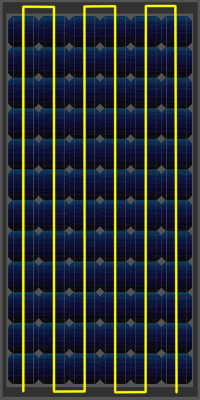
\includegraphics[width=40mm,height=80mm]{images/solar-facility/pvmodule-wiring.jpeg}
        };

        % Horizontal Measurement (Wires)
        % ==============================

        % Horizontal measurement between wires
        \draw (5mm,0mm) -- (5mm,4mm); % Vertical line
        \draw (11mm,0mm) -- (11mm,4mm);   % Vertical line

        % Measurement arrow
        \draw[-latex] (4mm,2mm) -- (5mm,2mm);
        \draw[-] (4mm,2mm) -- (31.5mm,2mm);
        \draw[latex-] (11mm,2mm) -- (12mm,2mm);

        % Measurment
        \node[anchor=west] at (12mm,3.75mm) {\small$d = \SI{127}{\milli\meter}$};


        % Vertical measurement (Wires)
        % ============================
        \draw (4mm,-1.5mm) -- (-4mm,-1.5mm); % horizontal line
        \draw (4mm,-78.5mm) -- (-4mm,-78.5mm); % horizontal line

        \draw[latex-latex] (-2mm,-1.5mm) -- (-2mm,-78.5mm); % measurement line

        % Measurement
        \node[rotate=90] at (-3.75mm,-38.5mm) {\small$l = \SI{1550}{\milli\meter}$};

        \node at (5mm,-82.5mm) {\small 1};
        \node at (11mm,-82.5mm) {\small 2};
        \node at (17mm,-82.5mm) {\small 3};
        \node at (23mm,-82.5mm) {\small 3};
        \node at (29mm,-82.5mm) {\small 2};
        \node at (35.5mm,-82.5mm) {\small 1};
    \end{scope}
\end{tikzpicture}


    \caption[PV-Modul, Modell f\"ur den Strompfad]{
        Solarmodul  gem\"ass Abbildung  \ref{fig:pvmodule} mit  Stromleitungen
        und  L\"angen   zur  Verbindung   der  Zellen. Die   Nummerierung  der
        Leiterbahnen   entspricht    der   Nummerierung    der   Koeffizienten
        in   Gleichungen   \ref{eq:rosa:a1}    bis   \ref{eq:rosa:a3}   (Seite
        \pageref{eq:rosa:a1}).%
    }
    \label{fig:pvmodule:wiring}
    \vspace*{-3em}
\end{wrapfigure}

Der  Pfad, den  der Strom  in  einem Modul  zur\"ucklegt, kann  je nach  Modul
mehrere Meter L\"ange  erreichen.  Dieser Effekt wird in  unserem Modell durch
eine Stromleitung modelliert, die \"uber  alle Zellen geht. In Realit\"at sind
die Leiter, welche die Zellen miteinander verbinden, ziemlich kurz (angenommen
die Zellen werden  von Kante zu Kante verbunden), aber  da der Strompfad durch
die ganze Zelle geht, wird der gesamte Strompfad in unserem Modell vereinfacht
als eine lange Leitung modelliert.

Zwischen   diesen   parallelen    Leiterbahnen   ergeben   sich   parasit\"are
Induktivit\"aten, die  im Folgenden  bestimmt und  in unser  Modell integriert
werden.  Die  angenommene Form und  die Abmessungen der  internen Stromleitung
sind  in  Abbildung   \ref{fig:pvmodule:wiring}  dargestellt. Die  Abmessungen
basieren auf folgenden Annahmen:

\begin{itemize}
    \tightlist
    \item
        Kantenl\"ange einer Zelle: \SI{125}{\milli\meter}
    \item
        Abstand zwischen zwei Modulen: \SI{2}{\milli\meter}
    \item
        \"Uberhang      am      oberen      und     unteren      Ende      des
        Moduls: \SI{14}{\milli\meter}
    \item
        Der Abstand  $d$ zweier Leiterbahnen ist  somit \SI{127}{\milli\meter}
        und
    \item
        die    L\"ange    $l$    einer   Leiterbahn    summiert    sich    auf
        \SI{1550}{\milli\meter}.
\end{itemize}


Zur  Berechnung  der  parasit\"aren  Induktivit\"at wird  \emph{The  Self  and
Mutual  Inductances  of Linear  Conductors}  von  Edward B. Rosa  herangezogen
\cite{ref:inductance:rosa}. Darin  wird   unter  anderem   die  Induktivit\"at
einer   Leiterkonfiguration  wie   sie  in   unserem  Modul   angenommen  wird
(Abbildung  \ref{fig:pvmodule:wiring}) bestimmt. Die  zugeh\"orige Formel  ist
in  Gleichung  \ref{eq:rosa:snake}  gegeben\footnotemark.
\footnotetext{%
    Die  Formeln  in   \cite{ref:inductance:rosa}  sind  im  \emph{CKG}-System
    (Centimeter,    Kilogramm,    Sekunden)     notiert,    f\"ur    Gleichung
    \ref{eq:rosa:snake} ist die Gleichung von  Rosa auf das SI-System normiert
    worden.%
}

\noindent Der  Wert f\"ur die Selbstinduktivit\"at  der verschiedenen Dr\"ahte
ist nicht  identisch; dies wird im  Summand $A_{\mathrm{i}}$ ber\"ucksichtigt,
der abh\"angt von der Anzahl  paralleler Leiterbahnen und ihrer Lage innerhalb
der  Leiteranordnung. F\"ur \num{6}  parallele Leiterbahnen  ergeben sich  die
Werte aus Gleichungen \ref{eq:rosa:a1}, \ref{eq:rosa:a2} und \ref{eq:rosa:a3}.


\begin{alignat}{2}
    \label{eq:rosa:snake}
    L &= \frac{\mu_{\mathrm{0}} \cdot l}{2 \cdot \pi}
    \cdot
    \left[
        \ln\left(
            \frac{d}{\rho}
        \right)
        + \frac{1}{4}
        - A_{\mathrm{i}}
    \right] & \quad \text{Selbstinduktivit\"at eines Leiters}
    \\
    \label{eq:rosa:a1}
    A_{\mathrm{1}} &= -\ln\left(\frac{15}{8}\right) & \text{\"ausserste Leiterbahnen} \\
    \label{eq:rosa:a2}
    A_{\mathrm{2}} &= \ln\left(\frac{16}{5}\right)  & \text{Leiterbahnen Nr. 2} \\
    \label{eq:rosa:a3}
    A_{\mathrm{3}} &= \ln\left(\frac{4}{3}\right)   & \text{Leiterbahnen Nr. 3, Mitte}
\end{alignat}

\begin{conditions}
    d              & Abstand zwischen zwei Leiterbahnen \\
    \rho           & Radius des Leiters \\
    A_{\mathrm{i}} & Korrektursummand f\"ur Leiterposition gem\"ass Abbildung \ref{fig:pvmodule:wiring} \\
\end{conditions}

Somit kann f\"ur  jeden Teil der Leitung in einem  Modul dessen Induktivit\"at
berechnet  werden. Diese  werden  anschliessend summiert  (Serieschaltung  von
Induktivit\"aten) und  als Gesamtinduktivit\"at  eines Moduls in  unser Modell
integriert.

Es   wird  von   einem   Leiterquerschnitt  von   \SI{4}{\milli\meter\squared}
ausgegangen,  was  einen   Leiterradius  $\rho$  von  \SI{1.128}{\milli\meter}
ergibt. Dies ist eine g\"angige Gr\"osse in PV-Installationen.

Die  Induktivit\"aten der  Leiterbahnen  innerhalb des  Moduls k\"onnen  somit
bestimmt werden:

\begin{alignat}{2}
    L_{\mathrm{1}} &= \frac{\mu_{\mathrm{0}} \cdot l}{2 \cdot \pi}
    \cdot
    \left[
        \ln\left(
            \frac{d}{\rho}
        \right)
        + \frac{1}{4}
        - A_{\mathrm{1}}
    \right]
    & = \SI{1.737}{\micro\henry} \\
    L_{\mathrm{2}} &= \frac{\mu_{\mathrm{0}} \cdot l}{2 \cdot \pi}
    \cdot
    \left[
        \ln\left(
            \frac{d}{\rho}
        \right)
        + \frac{1}{4}
        - A_{\mathrm{2}}
    \right]
    & = \SI{1.181}{\micro\henry} \\
    L_{\mathrm{3}} &= \frac{\mu_{\mathrm{0}} \cdot l}{2 \cdot \pi}
    \cdot
    \left[
        \ln\left(
            \frac{d}{\rho}
        \right)
        + \frac{1}{4}
        - A_{\mathrm{3}}
    \right]
    & = \SI{1.453}{\micro\henry}
\end{alignat}

\begin{conditions}
    \mu_{\mathrm{0}} = 4 \cdot \pi \cdot 10^{-7} & magnetische Permeabilit\"at des Vakuums \\
    l                = \SI{1550}{\milli\meter}   & L\"ange einer Leiterbahn                \\
    d                = \SI{127}{\milli\meter}    & Abstand zweier Leiterbahnen             \\
    \rho             = \SI{1.128}{\milli\meter}  & Radius des Leiters                      \\
    A_{\mathrm{1}}   =  -0.6286                  & Korrektursummand                        \\
    A_{\mathrm{2}}   =   1.1632                  & Korrektursummand                        \\
    A_{\mathrm{3}}   =   0.2877                  & Korrektursummand                        \\
\end{conditions}

\clearpage
Die Gesamtinduktivit\"at der Leiterbahnen in einem Modul ist somit:

\begin{equation}
    \label{eq:pvmodule:totalInductance}
    \underline{\underline{L_{\mathrm{Modul}}
    =
    2 \cdot \left(
        L_{\mathrm{1}} + L_{\mathrm{2}} + L_{\mathrm{3}}
    \right)
    = \SI{8.74}{\micro\henry}}}
\end{equation}

Es bleibt noch der Ohm'sche Widerstand der Leiterbahn zu bestimmen\footnotemark.
Dieser errechnet sich zu:

\footnotetext{%
    Es  sei  an   dieser  Stelle  darauf  hingewiesen,  dass   der  im  Modell
    der  Solarzelle  vorkommende  Seriewiderstand $R_{\mathrm{S}}$  nicht  die
    Leiterbahnen modelliert, sondern thermische Verluste im Halbleitersubstrat
    \cite{pvcell:masmoudi}%
}

\begin{equation}
    \label{eq:resistance:ohm:module}
    \underline{\underline{R = \frac{\rho \cdot l}{A} = \SI{44.2}{\milli\ohm}}}
\end{equation}

\begin{conditions}
    A = \SI{4}{\milli\meter\squared} & Querschnittsfl\"ache des Leiters \\
    \rho = \SI{0.0178}{\ohm\milli\meter\squared\per\meter} & Spezifischer Widerstand Leitungskupfer \cite{ref:kuchling:rhoCu} \\
    l = (6 \cdot 1550 + 5 \cdot 127)\si{\milli\meter} = \SI{9.935}{\meter} & Gesamtl\"ange des Leiters in einem Modul \\
\end{conditions}

Mit  diesen Informationen  kann  das Schaltbild  f\"ur  ein PV-Modul  bestimmt
werden,  was  die  Schaltung  in  Abbildung  \ref{fig:circuit:72x1:simplified}
ergibt. Dieses  Modell  wird im  Folgenden  benutzt,  um eine  Solaranlage  zu
modellieren.

\begin{figure}[h!tb]
    \centering
    % x: 0, 1, 3, 4
\def\POSxUp{0,3}
\def\POSxDown{1,4}
\def\POSy{0,1,3,4}
\begin{circuitikz}
    \foreach \x in \POSxUp{
        \foreach \y in \POSy {
            \draw
            (\x,\y) to[empty photodiode] (\x,\y+1)
            ;
        }
        \draw (\x,2.5) node[rotate=90] {\ldots};
    }
    \foreach \x in \POSxDown{
        \foreach \y in \POSy {
            \draw
            (\x,\y+1) to[empty photodiode] (\x,\y)
            ;
        }
        \draw (\x,2.5) node[rotate=90] {\ldots};
    }

    % Connecting Lines between Strings
    \draw (0,5) -- (1,5);
    \draw (1,0) -- (3,0);
    \draw (3,5) -- (4,5);

    \draw (0,0) -- (0,-0.5) node[ocirc] {~~IN};
    \draw (4,0) -- (4,-0.5) node[ocirc] {~~OUT};
\end{circuitikz}

    \caption[Ersatzschaltbild PV-Modul]{%
        Ersatzschaltbild   f\"ur  das   PV-Modul. Es   besteht  einem   Strang
        mit   72    Zellen   in   Serie   geschaltet    und   angeordnet   wie
        auf   dem   Modul   in    Abbildung   \ref{fig:pvmodule}   auf   Seite
        \pageref{fig:pvmodule}.     Zus\"atzlich    ist    die    parasit\"are
        Induktivit\"at  der Leiterbahnen  im Modul  ber\"ucksichtigt und  eine
        Freilaufdiode integriert.  Die vollst\"andige \code{LTspice}-Schaltung
        ist   in   Abbildung   \ref{fig:ltspice:jacModule:Diode}   auf   Seite
        \pageref{fig:ltspice:jacModule:Diode} dargestellt.%
    }
    \label{fig:circuit:72x1:simplified}
\end{figure}



% ---------------------------------------------------------------------------- %
\section{Modellierung eines Modulstrangs}
\label{sec:simu:model:module:string}
% ---------------------------------------------------------------------------- %

Der zu  simulierende Modulstrang soll  aus 20  Modulen bestehen, die  in Serie
miteinander  verbunden werden. Die  Induktivit\"at der  Leitungen, welche  die
Module  miteinander verbinden,  wird  vernachl\"assigt,  da die  zugeh\"origen
Distanzen  zwischen den  Leitern viel  gr\"osser sind,  als die  Distanzen der
Leiterbahnen innerhalb eines Moduls (siehe vorheriger Abschnitt).

Es  soll  jedoch  die  Induktivit\"at  der  Anschlussleitung  ber\"ucksichtigt
werden. Dabei   soll  von   einem   \SI{20}{\meter}  langen   Doppelleiterpaar
ausgegangen  werden, das  in einem  Abstand von  \SI{20}{\milli\meter} verlegt
worden ist. Dies ist nat\"urlich eine  idealisierte Annahme; in der Realit\"at
sind  diese Leiter  weder mit  konstant gleichem  Abstand noch  perfekt gerade
verlegt.

Die  von   Rosa  in  \cite{ref:inductance:rosa}  gegebene   Formel  f\"ur  die
Induktivit\"at eines geraden, parallelen Leiterpaares lautet\footnotemark:

\footnotetext{%
    Auch  hier  ist  Rosa's  Formel  auf  das  moderne  SI-System  konvertiert
    worden. Zudem wird  davon ausgegangen,  dass die  Leiter aus  Kupfer sind.
    Dessen  relative  Permeabilit\"at  $\mu_{\mathrm{r}}$  liegt  bei  etwa  1
    \cite{ref:kuchling:muRCu} und kann somit in der Gleichung vernachl\"assigt
    werden.

    Auch Kuchling gibt in \cite{ref:Kuchling:Ltwo} die gleiche Formel.%
}

\begin{equation}
    \label{eq:rosa:dualwire}
    \underline{\underline{L = \frac{\mu_{0}}{\pi} \cdot \left[ \ln\left(\frac{d}{\rho}\right) + \frac{1}{4} \right]
    = \SI{25}{\micro\henry}}}
\end{equation}

\begin{conditions}
    \mu_{\mathrm{0}} = 4 \cdot \pi \cdot 10^{-7} & magnetische Permeabilit\"at des Vakuums \\
    l                = \SI{20}{\meter}           & L\"ange des Leiterpaares (ein Weg)    \\
    d                = \SI{20}{\milli\meter}     & Abstand der Leiter                    \\
    \rho             = \SI{1.128}{\milli\meter}  & Radius des Leiters                    \\
\end{conditions}

Da zwei parallel  verlaufende Leiter im Prinzip  einen Kondensator darstellen,
soll  an  dieser  Stelle  auch   die  parasit\"are  Kapazit\"at  der  zu-  und
wegf\"uhrenden Leiterbahnen ber\"ucksichtigt werden. Die Formel zur Berechnung
dieser Kapazit\"at ist gem\"ass Kuchling \cite{ref:Kuchling:CTwo}:

\begin{equation}
    \label{eq:rosa:dualwire}
    \underline{\underline{C = \frac{\pi \cdot \epsilon_{0} \cdot \epsilon_{\mathrm{r}} \cdot l}{\ln\left(\frac{d}{\rho}\right)}
    = \SI{193.5}{\pico\farad}}}
\end{equation}

\begin{conditions}
    \epsilon_{0} = \SI{8.854}{\pico\farad\per\meter} & Elektrische Feldkonstante          \\
    \epsilon_{\mathrm{r}} = 1                        & Permittivit\"atszahl von Luft      \\
    l                = \SI{20}{\meter}               & L\"ange des Leiterpaares (ein Weg) \\
    d                = \SI{20}{\milli\meter}         & Abstand der Leiter                 \\
    \rho             = \SI{1.128}{\milli\meter}      & Radius des Leiters                 \\
\end{conditions}

\clearpage
Der Ohm'sche Widerstand der Anschlussleitung errechnet sich zu:

\begin{equation}
    \label{eq:resistance:ohm:module}
    \underline{\underline{R = \frac{\rho \cdot l}{A} = \SI{178}{\milli\ohm}}}
\end{equation}

\begin{conditions}
    A    = \SI{4}{\milli\meter\squared} & Querschnittsfl\"ache des Leiters \\
    \rho = \SI{0.0178}{\ohm\milli\meter\squared\per\meter} & Spezifischer Widerstand Leitungskupfer \cite{ref:kuchling:rhoCu} \\
    l    = \SI{40}{\meter} & Gesamtl\"ange der Anschlussleitung (beide Wege) \\
\end{conditions}

\vspace*{3em}
\begin{figure}[h!tb]
    \centering
    \def\POSx{9,8,7,6,5,4,3,2,1,0}
%\def\POSxRight{2,3,4,5,6,7,8,9,10,11}
\begin{circuitikz}
    %(12,0) -- (10,0)

    % Right to Left
    \foreach \x in \POSx {
        \draw
        (\x,1.5) to[empty photodiode] (\x - 1,1.5)
        ;
    }

    % Left to Right
    \foreach \x in \POSx {
        \draw
        (\x-1,-1.5) to[empty photodiode] (\x,-1.5)
        ;
    }

    % Endpoints
    \draw (-1,1.5) -- (-1,-1.5);

    % Stuff on the right
    \draw (9,1.5)  -- (9,0.75)  to[L,l^=L] (12,0.75)  node[ocirc] { };
    \draw (9,-1.5) -- (9,-0.75) to[R,l_=R] (12,-0.75) node[ocirc] { };
    \draw (9.5,0.75) node[circ] { } to[C,l^=C] (9.5,-0.75) node[circ] { };
\end{circuitikz}

    \caption[Ersatzschaltbild Modulstrang mit Verbindungsleitung]{
        Modell  eines Modulstrangs  aus  20 seriell  geschalteten Modulen  mit
        Ber\"ucksichtigung der Resistivit\"at,  Induktivit\"at und Kapazit\"at
        einer \SI{20}{\meter} langen Zuleitung%
    }
    \label{fig:pvstring}
\end{figure}

\vspace*{3em}
Abbildung  \ref{fig:pvstring} zeigt  das  Ersatzschaltbild eines  Modulstrangs
aus    20   in    Serie   geschalteten    Modulen   mit    den   parasit\"aren
Leiterimpedanzen. Dieses  und  die  vorangegangenen   Modelle  werden  nun  in
\code{LTspice} implementiert und f\"ur Simulationen benutzt.
            % DEPRECATED
%% **************************************************************************** %
\chapter{\code{LTspice} Schaltung eines Photovoltaik-Moduls}
\label{app:simu:module}
% **************************************************************************** %

\fref{fig:ltspice:solarCell}   zeigt   die  Implementation   unseres   Modells
einer     Solarzelle      gem\"ass     \fref{fig:circuit:solarCell}     (Seite
\pageref{fig:circuit:solarCell} in Abschnitt \ref{subsubsec:hw:ask:modell}) in
\code{LTspice}.

Ein MOSFET  wird benutzt, um  die Zelle  gesteuert (in unserer  Simulation bei
einer Tr\"agerfrequenz von \SI{10}{\kilo\hertz}) kurzschliessen zu k\"onnen.

Es    soll   das    f\"ur   den    MOSFET   schlimmere    Szenario   evaluiert
werden   (mehr    Strom/Leistung   durch    den   MOSFET\todo{Korrekt?}). Dazu
werden   aus  72   Zellen  zwei   verschiedene  Module   aufgebaut: Ein  Modul
\"ahnlich    zum    Sunset   Solargenerator    AS150    \cite{ref:solar:as150}
mit    ca. \SI{10}{\ampere}   Kurzschlussstrom    und   etwa    \SI{22}{\volt}
Leerlaufspannung  (\fref{fig:ltspice:module:cellBased:36x2}),  und  ein  Modul
\"ahnlich  zum Sunmodule  Pro-Series  XL SWB320  \cite{ref:solar:sunmodulePro}
mit   \SI{10}{\ampere}   Kurzschlussstrom    und   ungef\"ahr   \SI{45}{\volt}
Leerlaufspannung (\fref{fig:ltspice:module:cellBased:72x1}).

Weil die gesamte Kapazit\"at bei in Serie geschalteten Kondensatoren sinkt und
bei  paralleler  Anordnung steigt,  hat  die  $2 \times  36$-Parallelschaltung
\todo{Bindestrich und Spaces?} etwa die doppelte Kapazit\"at des Einzelstrangs
aus 72 Zellen. Der  durch den MOSFET fliessende Stroms, die  \"uber den MOSFET
abfallende Spannung und die im  MOSFET dissipierte Leistung beim Durchschalten
des Transistors sollen zwischen den beiden Szenarien verglichen werden.

Die zu  diesen Schaltungen geh\"orenden \code{.asc}-Dateien  sind elektronisch
verf\"ugbar  (Datentr\"ager  siehe Anhang  \ref{app:electronicStorage},  Seite
\pageref{app:electronicStorage}).

\begin{figure}[h!tb]
    \centering
    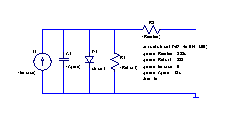
\includegraphics[width=\textwidth]{images/ltspice/singlecell.eps}
    \caption{%
        Schaltung        zur         Simulation        einer        Solarzelle
        gem\"ass        Abbildung       \ref{fig:circuit:solarCell}        von
        Seite     \pageref{fig:circuit:solarCell}. Die     Solarmodule     aus
        den     Abbildungen    \ref{fig:ltspice:module:cellBased:36x2}     und
        \ref{fig:ltspice:module:cellBased:72x1}  basieren auf  Zellen gem\"ass
        diesem Schaltschema.%
    }
    \label{fig:ltspice:solarCell}
\end{figure}

\begin{figure}[h!tb]
    \centering
    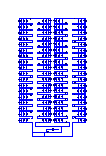
\includegraphics[width=\textwidth]{images/ltspice/module-72cells.eps}
    \caption{%
        Solarmodul     \"ahnlich     zu    Sunset     Solargenerator     AS150
        \cite{ref:solar:as150}, modelliert durch 2  parallele Str\"ange mit je
        36 Zellen gem\"ass Abbildung \ref{fig:ltspice:solarCell} in Serie.%
    }
    \label{fig:ltspice:module:cellBased:36x2}
\end{figure}

\begin{figure}[h!tb]
    \centering
    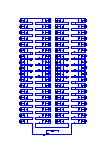
\includegraphics[width=\textwidth]{images/ltspice/module-72cells-series.eps}
    \caption{%
        Solarmodul   \"ahnlich   zu   Sunmodule  Pro-Series   XL   SW320   aus
        \cite{ref:solar:sunmodulePro},  modelliert durch  einen Strang  mit 72
        Zellen gem\"ass Abbildung \ref{fig:ltspice:solarCell} in Serie.%
    }
    \label{fig:ltspice:module:cellBased:72x1}
\end{figure}
\todo{Transistoren aus Schaltbildern entfernen, IN/OUT benennen, Abbildung sollte nur Modul sein}
        % DEPRECATED
%% **************************************************************************** %
\chapter{Erg\"anzende Simulationsergebnisse}
\label{app:simu:complementary}
% **************************************************************************** %


Dieses   Kapitel  beinhaltet   erg\"anzende  Simulationsergebnisse,   die  aus
Gr\"unden der \"Ubersichtlichkeit nicht im Hauptteil zu finden sind.


% ---------------------------------------------------------------------------- %
\section{Modul mit zwei parallelen Str\"angen}
\label{app:sec:simu:complementary:36x2}
% ---------------------------------------------------------------------------- %

\begin{figure}[h!tb]
    \centering
    \begin{tikzpicture}
       \begin{scope}[x={(0mm,0mm)},y={(120mm,0.95\textwidth)}]
           \begin{axis}[%
                   height=40mm,
                   width=\textwidth,
                   at={(0,70mm)},
                   grid=both,
                   xlabel=Zeit (\si{\micro\second}),
                   ylabel=Strom (\si{\ampere}),
                   %x unit=u,
                   change x base=true,
                   x SI prefix=micro,
               ]
               \addplot[-,color=blue] table {data/module-72cells--I-MOSFET--1000u.dat};
           \end{axis}
           \begin{axis}[%
                   height=40mm,
                   width=\textwidth,
                   at={(0,35mm)},
                   grid=both,
                   xlabel=Zeit (\si{\micro\second}),
                   ylabel=Spannung (\si{\volt}),
                   %x unit=u,
                   change x base=true,
                   x SI prefix=micro,
               ]
               \addplot[-,color=magenta] table {data/module-72cells--U-MOSFET--1000u.dat};
           \end{axis}
           \begin{axis}[%
                   height=40mm,
                   width=\textwidth,
                   at={(0,0)},
                   grid=both,
                   xlabel=Zeit (\si{\micro\second}),
                   ylabel=Leistung (\si{\watt}),
                   %x unit=u,
                   change x base=true,
                   x SI prefix=micro,
               ]
               \addplot[-,color=teal] table {data/module-72cells--P-MOSFET--1000u.dat};
           \end{axis}
       \end{scope}
   \end{tikzpicture}
   \caption{%
       Transientensimulation des Kurzschlussverfahrens f\"ur ASK mit einem $36 \times 2$-Modul%
   }
\end{figure}
\todo{``Abbilddung sowieso auf Seite diesunddas ist ein vergr\"osserter Ausschnitt eines Peaks aus dieser Simulation''}


\begin{figure}[h!tb]
    \centering
    \begin{tikzpicture}
       \begin{scope}[x={(0mm,0mm)},y={(120mm,0.95\textwidth)}]
           \begin{axis}[%
                   height=40mm,
                   width=\textwidth,
                   at={(0,70mm)},
                   grid=both,
                   xlabel=Zeit (\si{\micro\second}),
                   ylabel=Strom (\si{\ampere}),
                   %x unit=u,
                   change x base=true,
                   x SI prefix=micro,
               ]
               \addplot[-,color=blue] table {data/module-72cells-series--I-MOSFET--1000u.dat};
           \end{axis}
           \begin{axis}[%
                   height=40mm,
                   width=\textwidth,
                   at={(0,35mm)},
                   grid=both,
                   xlabel=Zeit (\si{\micro\second}),
                   ylabel=Spannung (\si{\volt}),
                   %x unit=u,
                   change x base=true,
                   x SI prefix=micro,
               ]
               \addplot[-,color=magenta] table {data/module-72cells-series--U-MOSFET--1000u.dat};
           \end{axis}
           \begin{axis}[%
                   height=40mm,
                   width=\textwidth,
                   at={(0,0)},
                   grid=both,
                   xlabel=Zeit (\si{\micro\second}),
                   ylabel=Leistung (\si{\watt}),
                   %x unit=u,
                   change x base=true,
                   x SI prefix=micro,
               ]
               \addplot[-,color=teal] table {data/module-72cells-series--P-MOSFET--1000u.dat};
           \end{axis}
       \end{scope}
   \end{tikzpicture}
   \caption{%
       Transientensimulation des Kurzschlussverfahrens f\"ur ASK mit einem $72 \times 1$-Modul%
   }
\end{figure}

\todo{``Abbilddung sowieso ist ein vergr\"osserter Ausschnitt eines Peaks aus dieser Simualtin}

% **************************************************************************** %
\chapter{Elektronische Datentr\"ager}
\label{app:electronicStorage}
% **************************************************************************** %



% -------------------------------------------------------- %
% Page  numbering continues,  but chapter  numbers are  no %
% longer  displayed. See  memoir  documentation  for  more %
% information.                                             %
% -------------------------------------------------------- %
\backmatter

% -------------------------------------------------------- %
% Bibliography: We  are using  the  IEEEtran package  from %
% Michael Shell                                            %
%                                                          %
% There  are  a  few  different  styles  in  the  IEEEtran %
% package.   We are  going to  use  one of  two of  those, %
% either in the sorted or unsorted variety.                %
%                                                          %
% The sorted  version sorts  bibliographic entries  in the %
% bibliography alphabetically, while  the unsorted version %
% lists bibliographic  entries in the order  in which they %
% were cited (first occurrence).                           %
% -------------------------------------------------------- %
%\bibliographystyle{bibliography/IEEEtranS} % sorted
\raggedright
\bibliographystyle{bibliography/IEEEtran} % unsorted
\bibliography{bibliography/references}
\end{document}
